\bookpart{函数空间}{Function Spaces}
\label{part:function-spaces}

\BookPartGuide{%
信号、温度分布、回归函数和偏微分方程的解都是整个函数。比较两个这样的对象，用有限维向量的坐标已经不够：函数有无穷多个“坐标”，选用不同的误差度量，收敛与否的结论也会不同。本部分把函数当作无限维空间中的向量，研究这些空间的一般结构，以及表示、观测、变换和逼近函数的方法。

前四章建立共同结构。第~\ref{chap:functions-as-vectors}章对照有限维线性代数，说明无限项展开为何需要收敛条件、无限维中闭球为何不紧；第~\ref{chap:function-normed-spaces}章和第~\ref{chap:function-inner-product-spaces}章分别加入范数与内积，研究完备性、$L^p$空间、正交投影与正交展开；第~\ref{chap:function-class-covers}章问一类函数能否在给定精度下用有限张代表表覆盖，以及需要多少代表。

中间几章研究函数的表示与作用。第~\ref{chap:fourier-transform}章和第~\ref{chap:wavelet-transform}章分别用频率和尺度给函数建立坐标；第~\ref{chap:linear-functionals}章研究积分、系数和点值等标量观测，第~\ref{chap:linear-operators}章把观测推广为函数之间的变换；第~\ref{chap:operator-spectra}章和第~\ref{chap:linear-operator-equations}章用谱与奇异系统分析算子，并讨论算子方程的可解性与稳定恢复；第~\ref{chap:function-approximation}章在给定误差和表示预算下比较各种逼近方式。

最后三章按具体问题选择函数空间：需要控制导数与边界时用第~\ref{chap:sobolev-spaces}章的Sobolev空间，需要区分不同尺度上的局部变化时用第~\ref{chap:besov-spaces}章的Besov空间，需要由离散点值观测函数时用第~\ref{chap:rkhs}章的再生核Hilbert空间。一般拓扑与度量的判据回用第~\ref{part:topology-and-metric}部分，积分工具回用第~\ref{part:measure}部分；拟合损失与正则化的选择留待机器学习笔记的回归内容讨论，给定目标后的优化求解由卷五介绍。}

\chapter{函数作为无限维向量}
\label{chap:functions-as-vectors}
\label{chap:function-spaces}

拟合一条曲线时，要比较的是两条完整的曲线；研究一列近似函数时，要问这一列整体上是否趋于某个函数。两件事都要求把一个完整的函数当作一个对象，对它做加法、做缩放、量距离。

这种看法可以从一列数开始。把函数$f$在一串输入$x_1,x_2,\ldots$处的取值排起来，就得到一个很长的向量：
\[
 f\ \longleftrightarrow\ [\ldots,a_1,a_2,a_3,\ldots],\qquad a_k=f(x_k).
\]
输入取得越密，这一列就越长。把所有输入都算上时，函数就成了一个“每个输入占一个分量”的向量，下标取遍定义域。本章的标题说的就是这件事。

卷二在有限维线性空间中建立了向量的语言：相加、数乘、基、坐标、范数。本章沿着上面的类比把这些概念逐一搬到函数上，每搬一个都问两个问题：它在函数上的对应物是什么，这个类比又在哪里失效。

第~\ref{sec:fvec-linear-operations}节说明函数的逐点运算正是向量的逐分量运算，由此得到函数空间。第~\ref{sec:fvec-dimension}节比较“定义域有多少点”与“空间有多少维”，这两个数并不相同：定义在整条实轴上、次数不超过$2$的多项式只组成三维空间。维数无限以后，有限线性组合不再够用，第~\ref{sec:fvec-infinite-expansions}节讨论用无穷多项之和表示元素时要回答哪些问题。第~\ref{sec:fvec-closed-ball-noncompact}节处理一个有限维中不会出现的现象：单位球里放得下无穷多个彼此远离的点。

本章只建立线性结构并指出无限维带来的困难。函数之间的范数、完备性及$L^p$空间在第~\ref{chap:function-normed-spaces}章研究；内积、正交投影和正交展开在第~\ref{chap:function-inner-product-spaces}章研究；有界函数类在给定精度下需要多少代表，在第~\ref{chap:function-class-covers}章研究。

\section{函数的线性运算}
\label{sec:fvec-linear-operations}

两条温度曲线可以取平均，一个信号可以整体放大一倍，一个近似函数减去目标函数得到误差函数。这些操作都作用于整个函数，结果仍是一个函数。它们遵守的规则与向量运算完全相同，原因就在于函数可以看成“每个输入占一个分量”的向量。

全章固定标量域$\mathbb K$，它是实数域$\mathbb R$或复数域$\mathbb C$。需要区分时，我们写明“实函数空间”或“复函数空间”；不写明时，结论对两种情形都成立。函数空间的元素是整个函数，按习惯用普通字母$f,g,h$或$x,y$表示，不用粗体。

\paragraph{逐点加法与数乘}
先做一个有限的计算。在$[0,1]$上取$f(x)=x^2$与$g(x)=1-x$，在四个等距点$x_1=0$、$x_2=\tfrac13$、$x_3=\tfrac23$、$x_4=1$处读出取值。每个函数由此变成一个四维向量：
\[
 \begin{aligned}
 [f(x_1),f(x_2),f(x_3),f(x_4)]&=[0,\tfrac19,\tfrac49,1],\\
 [g(x_1),g(x_2),g(x_3),g(x_4)]&=[1,\tfrac23,\tfrac13,0].
 \end{aligned}
\]
把这两个向量逐分量相加，得到
\[
 [1,\tfrac79,\tfrac79,1].
\]

函数$h(x)=x^2-x+1$在这四点的取值恰好是这四个数，而$h$正是在每个$x$处把$f(x)$与$g(x)$加起来的结果。所以“两个采样向量相加”与“两个函数在每个输入处相加”给出同一列数。

这个结论与采样点的个数无关。把四个点换成四十个、四百个，向量变长，每个分量上做的事不变。取遍全部输入时，就得到函数的加法。图~\ref{fig:fvec-pointwise-addition}左边是四维向量的相加，右边是取遍全部输入后的情形：在任何一个$x$处，把蓝色高度与绿色高度首尾相接，就落到$f+g$的曲线上。

\begin{BookInlineFigure}
  \centering
  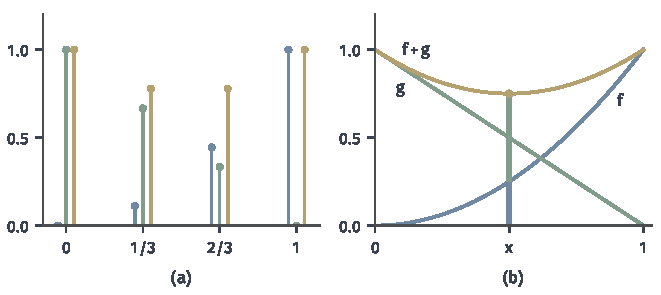
\includegraphics[width=112mm]{figures/04-spaces-measures-and-geometry/03-function-spaces/matplotlib/fvec-pointwise-addition/figure.pdf}
  \caption{函数相加就是逐分量相加。蓝色为$f(x)=x^2$，绿色为$g(x)=1-x$，黄色为二者之和。(a)四个采样点上的取值，每点从左到右依次是$f$、$g$、$f+g$的分量。(b)全部输入上的曲线；在一个固定的$x$处，蓝色线段与绿色线段接起来的总高度等于$f(x)+g(x)$。}
  \label{fig:fvec-pointwise-addition}
\end{BookInlineFigure}

现在写出一般的定义。固定一个非空集合$X$，称为输入集合，考虑全体函数$f:X\to\mathbb K$组成的集合，记为$\mathbb K^X$。这个记号本身就是类比：$\mathbb K^d$的元素给每个下标$k\in\{1,\ldots,d\}$指定一个数，$\mathbb K^X$的元素给每个$x\in X$指定一个数。两个函数的和与一个函数的数乘都在每个输入处分别计算：
\begin{equation}
 (f+g)(x)=f(x)+g(x),\qquad (cf)(x)=c\,f(x),
 \label{eq:fvec-pointwise-operations}
\end{equation}
其中$x\in X$，$c\in\mathbb K$。零元素是处处取零的\term{零函数}（zero function），$f$的负元是$x\mapsto-f(x)$。式~\eqref{eq:fvec-pointwise-operations}称为\term{逐点运算}（pointwise operations）。

逐点运算满足线性空间的八条运算规则，验证方法是把每条规则放到一个固定的输入处检查。以加法交换律为例，要证$f+g=g+f$，而两个函数相等的意思是它们在每个输入处取值相同。任取$x\in X$，由式~\eqref{eq:fvec-pointwise-operations}和数的交换律，
\[
 (f+g)(x)=f(x)+g(x)=g(x)+f(x)=(g+f)(x).
\]

结合律、分配律和零元、负元的规则都这样逐点继承自$\mathbb K$中的运算，所以$\mathbb K^X$在逐点运算下是$\mathbb K$上的线性空间。这与验证$\mathbb K^d$是线性空间时逐分量检查的做法相同。线性空间与子空间的一般定义、基与坐标，可参考\BookChapterRef{chap:linear-representation}{卷二第2章“线性空间、映射与坐标”}。

改变输入集合$X$，就得到熟悉的对象。取$X=\{1,\ldots,d\}$，函数就是$d$维向量。取$X=\mathbb N_+=\{1,2,3,\ldots\}$，一个函数$x:\mathbb N_+\to\mathbb K$就是一个数列$x=(x_1,x_2,\ldots)$，其中$x_k=x(k)$，式~\eqref{eq:fvec-pointwise-operations}这时是逐项相加与逐项数乘。取$X=[0,1]$，就是区间上的函数。图~\ref{fig:fvec-index-to-function}把这三种情形放在一起：横轴都是“下标”，纵轴都是“这个下标上的数”。

\begin{BookInlineFigure}
  \centering
  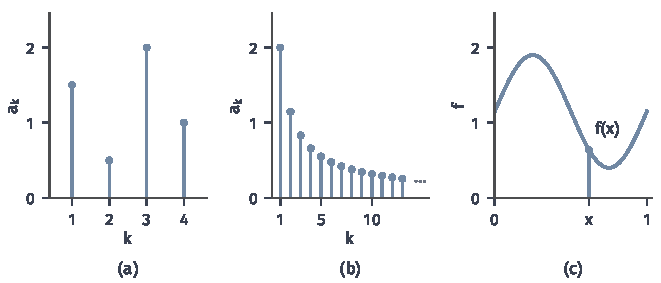
\includegraphics[width=112mm]{figures/04-spaces-measures-and-geometry/03-function-spaces/matplotlib/fvec-index-to-function/figure.pdf}
  \caption{同一种构造的三个例子。(a)$X=\{1,2,3,4\}$时是四维向量。(b)$X=\mathbb N_+$时是数列，下标可以一直延伸下去。(c)$X=[0,1]$时下标连成一片，竖线所示的是下标$x$上的数$f(x)$，竖线的顶点连成了函数的图像。}
  \label{fig:fvec-index-to-function}
\end{BookInlineFigure}

类比在这里出现第一个边界。$X=[0,1]$时，输入有不可数个，无法排成$a_1,a_2,\ldots$这样的一列，所以$[\ldots,f(x),\ldots]$只是一幅图景，不是真的列表。好在式~\eqref{eq:fvec-pointwise-operations}用不着排序，它只要求对每个$x$分别计算。表~\ref{tab:fvec-dictionary}汇总了目前的对应关系。

\begin{BookInlineTable}
  \centering
  \begin{tabular}{@{}ll@{}}
    \toprule
    有限维向量$a\in\mathbb K^d$ & 函数$f\in\mathbb K^X$\\
    \midrule
    下标$k\in\{1,\ldots,d\}$ & 输入$x\in X$\\
    分量$a_k$ & 取值$f(x)$\\
    逐分量相加$a+b$ & 逐点相加$f+g$\\
    逐分量数乘$ca$ & 逐点数乘$cf$\\
    零向量 & 零函数\\
    $a=b$：每个分量相等 & $f=g$：每个输入处取值相等\\
    \bottomrule
  \end{tabular}
  \caption{有限维向量与函数的对应。左右两列的运算规则相同，差别只在下标集合。}
  \label{tab:fvec-dictionary}
\end{BookInlineTable}

\paragraph{线性子空间的核验}
实际使用的通常不是全体函数，而是满足某种要求的函数，例如连续函数或多项式。这就像在$\mathbb R^3$中只看一个过原点的平面。要在这样的集合$V\subseteq\mathbb K^X$中继续使用线性空间的语言，须核对三条：零函数属于$V$；$V$中两个函数之和仍在$V$中；$V$中函数的数乘仍在$V$中。三条都成立时，$V$是$\mathbb K^X$的线性子空间，本身也是线性空间，下面简称为\term{函数空间}（function space）。

几个常用的集合都通过了核验。闭区间上的连续函数全体$C[a,b]$是线性子空间，因为常数零连续，连续函数的和与数乘仍连续。次数不超过$m$的多项式全体$P_m$是线性子空间，因为两个这样的多项式相加不会提高次数。

数列也有同样的例子。收敛到零的数列全体记为$c_0$，它是线性子空间：若$x_k\to0$、$y_k\to0$，则$x_k+y_k\to0$，$cx_k\to0$。只有有限项非零的数列全体记为$c_{00}$，它也是线性子空间，因为两个数列的非零项都只有有限个时，和的非零项也只有有限个。

约束一个分量的取值，能看出子空间与非子空间的区别。集合$\{f\in C[0,1]:f(0)=0\}$把“下标$0$上的分量”固定为零，它是线性子空间，正如$\mathbb R^3$中的平面$x_1=0$。集合$\{f\in C[0,1]:f(0)=1\}$则对应不过原点的平面$x_1=1$：它不含零函数，两个成员相加后在$0$处取$2$，也不封闭。

失败还可以更隐蔽。$\mathbb R^2$中两条坐标轴的并集对数乘封闭，但$(1,0)+(0,1)$已经离开了这个集合。函数空间中也有同样的情形，考虑参数族
\[
 \mathcal R=\{x\mapsto a\max(0,x-t):a,t\in\mathbb R\},
\]
其中每个成员的图像是一条折线，斜率至多改变一次。

取$\mathcal R$中的两个成员$f(x)=\max(0,x)$与$g(x)=\max(0,x-1)$，分段写出它们的和：
\[
 (f+g)(x)=\begin{cases}0,&x\leq0,\\x,&0<x\leq1,\\2x-1,&x>1.\end{cases}
\]
斜率在$x=0$处由$0$变为$1$，在$x=1$处由$1$变为$2$，共改变两次，所以$f+g\notin\mathcal R$。$\mathcal R$对数乘封闭、对加法不封闭，和两条坐标轴的并集属于同一类。这样的族可以作为逼近工具，但不能直接当作线性空间使用。

\paragraph{函数值、函数元素与坐标}
向量有下标$k$、分量$a_k$和整个向量$a$三个层次，函数也一样。输入$x\in X$是一个位置；$f(x)\in\mathbb K$是这个位置上的数；$f$本身是整条对应规则，是函数空间中的一个元素。说“$f=g$”是在比较元素，要求所有位置的值都相同；说“$f(x_0)=g(x_0)$”只比较了一个位置。

坐标是另一回事，它依赖另外选定的基。在$P_2$中取多项式$p(x)=2-x+3x^2$，相对于基$1,x,x^2$，它的坐标是系数$(2,-1,3)$。改用基$1,x-1,(x-1)^2$时，要把$p$按$x-1$重新整理。令$t=x-1$，把$x=t+1$代入$p$，得到
\[
 p=2-(t+1)+3(t+1)^2.
\]
展开平方并合并同类项，得到
\[
 p=4+5t+3t^2.
\]
换回$x$，就是
\[
 p(x)=4+5(x-1)+3(x-1)^2,
\]
所以新的坐标是$(4,5,3)$。

元素$p$没有变，变的是记录它的方式。这与卷二中同一个向量在两组基下有两列坐标是一回事。图~\ref{fig:fvec-two-coordinates}中两张图的蓝色曲线是同一条，只是拆成了不同的三个部分。

\begin{BookInlineFigure}
  \centering
  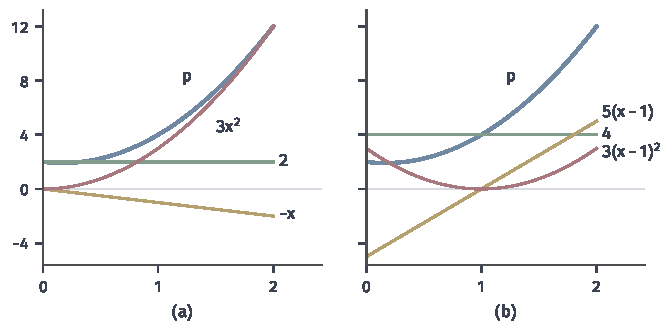
\includegraphics[width=112mm]{figures/04-spaces-measures-and-geometry/03-function-spaces/matplotlib/fvec-two-coordinates/figure.pdf}
  \caption{同一个函数的两种分解。蓝色曲线都是$p(x)=2-x+3x^2$。(a)拆成$2$、$-x$、$3x^2$三部分，坐标为$(2,-1,3)$。(b)拆成$4$、$5(x-1)$、$3(x-1)^2$三部分，坐标为$(4,5,3)$。在每个$x$处，同一张图中三条细线的高度之和等于蓝色曲线的高度。}
  \label{fig:fvec-two-coordinates}
\end{BookInlineFigure}

函数值$p(1)=4$恰好等于第二组坐标的第一项，因为另外两个基函数在$x=1$处都为零。这是这组基的性质，不是坐标的一般含义：第一组坐标的第一项$2$等于$p(0)$，并不等于$p(1)$。

至此，一个函数有了两种“一列数”。一种是取值列，下标是输入$x$，它不需要选基。另一种是系数列，下标是基函数的编号，它随基改变。本章开头的$[\ldots,a_1,a_2,\ldots]$可以按这两种方式来读，下一节会把二者的关系写成矩阵。

\paragraph{乘法与微分不是一般的内部运算}
向量也可以逐分量相乘，但线性空间的定义用不到这种运算。函数同样如此：逐点乘法$(fg)(x)=f(x)g(x)$在某些集合上有意义，却不属于线性结构。$P_m$对乘法不封闭，因为$x^m\in P_m$，而$x^m\cdot x=x^{m+1}\notin P_m$。

求导$f\mapsto f'$也要看空间。$C[0,1]$对乘法封闭，对求导却不封闭：$f(x)=\lvert x-\tfrac12\rvert$连续，但在$\tfrac12$处不可导，$f'$不是$[0,1]$上处处有定义的函数。

所以讨论某个函数空间时，加法与数乘是自带的运算；乘积和导数是另外的操作，要单独说明它们从哪个空间送到哪个空间。例如求导把$P_2$送入$P_2$，而且是线性的。若用基$1,x,x^2$的坐标表示，把$a_0+a_1x+a_2x^2$求导得到$a_1+2a_2x$，这个操作就是一个矩阵：
\[
 \begin{bmatrix}a_1\\2a_2\\0\end{bmatrix}
 =\begin{bmatrix}0&1&0\\0&0&2\\0&0&0\end{bmatrix}
 \begin{bmatrix}a_0\\a_1\\a_2\end{bmatrix}.
\]

把前面的$(2,-1,3)$代入，得到$(-1,6,0)$，也就是$p'(x)=-1+6x$。乘一个固定函数$g$的操作也有这样的矩阵形式：在采样点上，它是对角元为$g(x_1),\ldots,g(x_n)$的对角矩阵。这样的映射在无限维空间中称为线性算子，在第~\ref{chap:linear-operators}章研究；可微性的推广则由第~\ref{chap:smoothing-weak-derivatives}章的弱导数承担。

\section{函数空间的维数}
\label{sec:fvec-dimension}

线性空间的维数是张成整个空间所需的最少方向数，也就是一组基中元素的个数。函数空间的维数同样按这个定义计算。困难在于函数还带着一个输入集合，容易让人把“输入有多少个点”误当成“空间有多少维”。类比$[\ldots,f(x),\ldots]$提示每个输入占一个分量，但下面会看到，只有输入集合有限时，点数才恰好等于$\mathbb K^X$的维数；一般的函数空间只取其中一部分函数，维数可以远小于点数。

\subsection{有限维函数空间}
\label{sec:fvec-finite-dimensional}

最直接的有限维函数空间来自有限的输入集合。设$X=\{x_1,\ldots,x_m\}$有$m$个不同的点。一个函数$f:X\to\mathbb K$由它的$m$个取值$f(x_1),\ldots,f(x_m)$完全确定，所以我们期望$\mathbb K^X$与$\mathbb K^m$是同一个空间的两种写法。

\paragraph{指示函数基}
$\mathbb K^m$的标准基$e_i$在第$i$个分量上取$1$，其余分量取$0$。把这句话照搬到函数上，就是为每个点准备一个只在该点取$1$的函数，即\term{指示函数}（indicator function）
\[
 \delta_i(x)=\begin{cases}1,&x=x_i,\\0,&x\neq x_i,\end{cases}\qquad i=1,\ldots,m.
\]

任意$f\in\mathbb K^X$都可以写成这些函数的组合：
\begin{equation}
 f=\sum_{i=1}^mf(x_i)\,\delta_i.
 \label{eq:fvec-indicator-expansion}
\end{equation}
验证方法是比较两边在每个$x_j$处的取值。右边求和时，只有$i=j$的一项不为零，所以右边在$x_j$处等于$f(x_j)$，与左边相同。于是$\delta_1,\ldots,\delta_m$张成$\mathbb K^X$。

这组函数也线性无关。设$\sum_ic_i\delta_i$是零函数，在$x_j$处取值，得到
\[
 c_j=\sum_{i=1}^mc_i\delta_i(x_j)=0,
\]
这对每个$j$都成立。所以$\delta_1,\ldots,\delta_m$是一组基，$\dim\mathbb K^X=m$。式~\eqref{eq:fvec-indicator-expansion}说明，$f$在这组基下的坐标恰好是它的$m$个取值。

这时函数的线性运算完全变成坐标运算。取$X=\{0,1,2\}$，设$f$与$g$的取值分别是下面两列数：
\[
 f=(1,0,4),\qquad g=(2,-1,1).
\]
式~\eqref{eq:fvec-pointwise-operations}在每点分别计算，于是$2f-g$的取值是
\[
 2f-g=(2\cdot1-2,\ 2\cdot0+1,\ 2\cdot4-1)=(0,1,7).
\]
这三个数也就是$2f-g$的坐标。图~\ref{fig:fvec-indicator-basis}把$f$拆成了三个指示函数的高度，与把$\mathbb K^3$的向量拆成标准基是同一幅图。

\begin{BookInlineFigure}
  \centering
  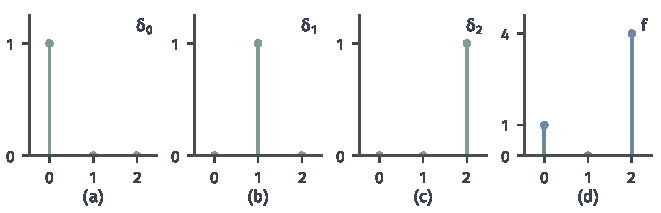
\includegraphics[width=112mm]{figures/04-spaces-measures-and-geometry/03-function-spaces/matplotlib/fvec-indicator-basis/figure.pdf}
  \caption{$X=\{0,1,2\}$上的指示函数基。(a)至(c)是三个基函数$\delta_0,\delta_1,\delta_2$，每个只在一个输入处取$1$。(d)是$f=\delta_0+4\delta_2$，它的三个取值$(1,0,4)$就是坐标。}
  \label{fig:fvec-indicator-basis}
\end{BookInlineFigure}

\paragraph{多项式基与坐标}
有限维函数空间不一定来自有限的输入集合。在整个实轴上考虑$P_m$，即次数不超过$m$的实多项式全体。每个$p\in P_m$可以写成
\[
 p(x)=a_0+a_1x+\cdots+a_mx^m,
\]
所以$1,x,\ldots,x^m$张成$P_m$。

要说明它们是一组基，还须核对线性无关。设$\sum_{k=0}^mc_kx^k$对每个实数$x$都等于零。左边是一个次数不超过$m$的多项式，若系数不全为零，它至多有$m$个根；而它在无穷多个点处取零，所以每个$c_k=0$。于是
\begin{equation}
 \dim P_m=m+1,
 \label{eq:fvec-polynomial-dimension}
\end{equation}
系数$(a_0,\ldots,a_m)$是$p$相对于这组基的坐标。

这个例子把两种“个数”分开了。$P_m$的定义域$\mathbb R$有不可数个点，空间却只有$m+1$维：一旦知道$m+1$个系数，整条曲线在每一点的值都确定了。可以想象一个不可数长的取值列，它的全部分量由$m+1$个数决定。维数只看张成整个空间需要多少方向，与函数定义在多少个点上无关。

在$P_2$上还可以把取值列与系数列的关系算清楚。上一节的$p(x)=2-x+3x^2$，系数列是$(2,-1,3)$。在三个点$0,1,2$处读取值，得到取值列
\[
 p(0)=2,\qquad p(1)=4,\qquad p(2)=12.
\]
一般地，对$a_0+a_1x+a_2x^2$在这三点取值，就是用一个矩阵乘系数列：
\begin{equation}
 \begin{bmatrix}p(0)\\p(1)\\p(2)\end{bmatrix}
 =\begin{bmatrix}1&0&0\\1&1&1\\1&2&4\end{bmatrix}
 \begin{bmatrix}a_0\\a_1\\a_2\end{bmatrix}.
 \label{eq:fvec-vandermonde}
\end{equation}

这个矩阵的行列式等于$(1-0)(2-0)(2-1)=2\neq0$，所以它可逆。这意味着系数列和取值列互相决定，$(2,-1,3)$与$(2,4,12)$只是同一个元素的两列坐标。图~\ref{fig:fvec-coefficient-point}把这三者放在一起：同一条抛物线，在两个坐标系中各是一个点。

\begin{BookInlineFigure}
  \centering
  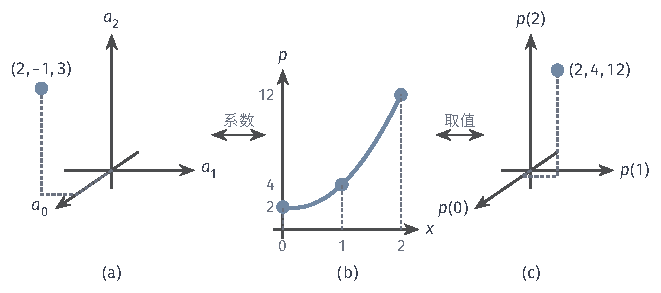
\includegraphics[width=111.919mm]{figures/04-spaces-measures-and-geometry/03-function-spaces/tikz/fvec-coefficient-point/figure.pdf}
  \caption{$P_2$中一个元素的三种面貌。(b)是曲线$p(x)=2-x+3x^2$，蓝点是它在$0,1,2$处的取值。(a)是它的系数列，在以系数为坐标轴的$\mathbb R^3$中是一个点。(c)是它在三点的取值列，在另一个$\mathbb R^3$中也是一个点。两个点由式~\eqref{eq:fvec-vandermonde}的矩阵互相转换。}
  \label{fig:fvec-coefficient-point}
\end{BookInlineFigure}

取值列也可以就是某组基下的坐标，只要选对基。令
\[
 \begin{aligned}
 \ell_0(x)&=\tfrac12(x-1)(x-2),\\
 \ell_1(x)&=-x(x-2),\\
 \ell_2(x)&=\tfrac12x(x-1).
 \end{aligned}
\]
这三个多项式在$0,1,2$上的取值分别是$(1,0,0)$、$(0,1,0)$、$(0,0,1)$，它们在这三点上的行为和指示函数一样。于是
\[
 p=2\ell_0+4\ell_1+12\ell_2.
\]
直接展开右边，得到$(x^2-3x+2)+(-4x^2+8x)+(6x^2-6x)$，合并后正是$2-x+3x^2$。

\subsection{无限维函数空间}
\label{sec:fvec-infinite-dimensional}

有限维向量的长度可以增加：$\mathbb R^1$可以看作$\mathbb R^2$中第二个分量为零的部分，$\mathbb R^2$又可以看作$\mathbb R^3$的一部分，这样一直延续下去。无限维说的是这个过程永远走不到头。若一个线性空间对每个正整数$n$都含有$n$个线性无关的元素，它就不能由任何有限个元素张成，称为\term{无限维}（infinite-dimensional）的。理由是卷二已经证明，由$k$个元素张成的空间中，线性无关的元素至多有$k$个。

\paragraph{全体多项式}
把次数的上限去掉，考虑全体实多项式组成的空间$P=\bigcup_{m\geq0}P_m$。它是线性子空间，因为两个多项式之和仍是多项式。上一小节的论证对每个$m$都成立，$1,x,\ldots,x^m$线性无关，而$m$可以任意大，所以$P$是无限维的。

也可以直接说明任何有限族都张不成$P$。设$q_1,\ldots,q_k$是有限个多项式，其中最高的次数为$d$。它们的任意线性组合次数都不超过$d$，所以$x^{d+1}$不在它们的张成空间中。无论选哪$k$个多项式，总有更高次的多项式落在外面。

\paragraph{全体数列}
数列空间$\mathbb K^{\mathbb N_+}$中，令$e_k$为第$k$项为$1$、其余各项为$0$的数列，称为第$k$个\term{标准单位列}（standard unit sequence），它是$\mathbb K^d$的标准基向量的直接延续。对任意$n$，若$\sum_{k=1}^nc_ke_k$是零数列，读出第$k$项即得$c_k=0$，所以$e_1,\ldots,e_n$线性无关。$n$任意，数列空间是无限维的。

同样的论证说明，只要输入集合$X$有无穷多个点，不同点的指示函数就构成任意多个线性无关的元素，$\mathbb K^X$都是无限维的。这里类比又碰到一个边界：$X$无限时，式~\eqref{eq:fvec-indicator-expansion}不能原样推广。指示函数的有限组合只在有限个点上不为零，所以常数函数$1$不在它们的张成空间中。取值仍然是每个输入上的数，却不再是一组基下的有限坐标。

\paragraph{每个元素有限与整体无限}
无限维并不意味着每个元素都“需要无穷多个方向”。$P$中的每个多项式只用到有限个单项式，它的系数列$[a_0,a_1,\ldots,a_d,0,0,\ldots]$从某一项起全为零；$c_{00}$中的每个数列也只是有限个$e_k$的组合。无限维说的是整个空间：没有一组固定的有限个方向，能同时表示所有元素。

图~\ref{fig:fvec-finite-support-grid}的前三行是三个多项式的系数列，每一行都只占有限个格子，但占到的最靠右的位置没有统一的上限。第四行不同：$e^x$的系数$1/k!$永远不为零。它不是多项式，因为任何多项式求导足够多次后变为零，而$e^x$求导后不变。

\begin{BookInlineFigure}
  \centering
  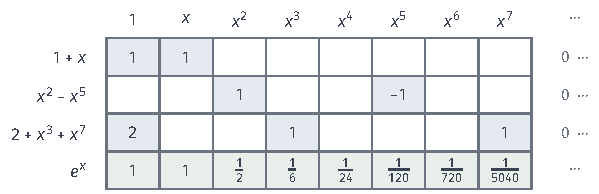
\includegraphics[width=101.469mm]{figures/04-spaces-measures-and-geometry/03-function-spaces/tikz/fvec-finite-support-grid/figure.pdf}
  \caption{系数列的两种形态。每一列对应一个单项式，蓝格是非零系数。前三行是多项式，只占有限个格子，其后全为零，所占范围随元素变化。第四行绿色的$e^x$每一格都不为零，有限个单项式的组合表示不了它。}
  \label{fig:fvec-finite-support-grid}
\end{BookInlineFigure}

数列空间中的常数列$(1,1,\ldots)$与$e^x$处境相同，它不是有限个$e_k$的组合。若想用$e_1,e_2,\ldots$表示这样的元素，就只能借助无穷多项之和，这需要先说明无穷和是什么意思。

\section{无限展开}
\label{sec:fvec-infinite-expansions}

有限维空间中，选定基以后，每个向量都由有限次加法和数乘精确地表示出来，坐标唯一，不涉及任何极限。进入无限维后，这一步分裂成两个问题：有限线性组合到底能覆盖哪些元素；对覆盖不到的元素，无穷多项的部分和能否趋于它，在什么意义下趋于它。数列的结构最简单，本节用数列把这两个问题分开研究，函数的正交展开要用到内积，在第~\ref{chap:function-inner-product-spaces}章讨论。

\subsection{代数基与级数表示}
\label{sec:fvec-algebraic-basis-series}

线性代数中的基只允许有限线性组合。把这一要求原样用于无限维空间，就得到下面的定义。

\begin{definition}[代数基]
\label{def:fvec-algebraic-basis}
设$V$是线性空间，$B\subseteq V$。若$B$中任意有限个不同元素线性无关，并且$V$的每个元素都是$B$中有限个元素的线性组合，称$B$为$V$的\term{代数基}（algebraic basis），也称\term{Hamel基}（Hamel basis）。
\end{definition}

定义中的两个条件各管一件事。线性无关保证表示唯一：若同一元素有两种有限表示，相减得到一个等于零的有限组合，各系数之差只能为零。“有限组合”则规定了允许的表示方式：不涉及任何极限，因此不需要事先给空间配上距离。

\paragraph{有限支撑数列与全体数列}
在$c_{00}$中，标准单位列$\{e_k\}_{k\geq1}$是代数基。线性无关上一节已经验证。若$x\in c_{00}$的非零项都在前$n$项之中，则
\[
 x=\sum_{k=1}^nx_ke_k
\]
是一个有限组合，所以$c_{00}$的每个元素都由$\{e_k\}$精确表示，坐标就是数列的各项。全体多项式$P$的情形相同：把多项式对应到它的系数列，$P$就成了换了名字的$c_{00}$，单项式$x^k$对应$e_{k+1}$。

同一族$\{e_k\}$在全体数列空间$\mathbb K^{\mathbb N_+}$中仍然线性无关，却不再张成整个空间。$e_1,\ldots,e_n$的任何组合从第$n+1$项起全为零，所以常数列$(1,1,\ldots)$不是有限个$e_k$的组合。$\{e_k\}$在$\mathbb K^{\mathbb N_+}$中只是一个线性无关族，它的有限组合恰好覆盖了$c_{00}$。

一般的无限维空间也有代数基，而且任何线性无关族都能扩充为一组代数基。证明要用到选择公理，具体通过Zorn引理进行，篇幅较长，读者可查阅线性代数或集合论的教材。这种存在性证明不给出具体的基，$\mathbb K^{\mathbb N_+}$的代数基至今没有可以写下来的公式。代数基仍然只允许有限组合，因此也不能用它谈论无穷和。

\paragraph{级数表示需要另外核对的内容}
要用$\{e_k\}$表示常数列这样的元素，自然想到写成无穷和$\sum_{k\geq1}x_ke_k$，把它理解为部分和
\[
 s_N=\sum_{k=1}^Nx_ke_k=(x_1,\ldots,x_N,0,0,\ldots)
\]
在$N\to\infty$时的极限。线性空间本身不提供极限，所以写下这个级数之前，先要规定“部分和趋于某个元素”的含义。

规定好收敛的意义之后，还要分别核对三件事。其一是收敛性：对给定的系数，部分和是否收敛。其二是表示范围：能够这样写出的元素是否覆盖整个空间。其三是唯一性：同一个元素能否有两组不同的系数。有限维时三者都自动成立，无限维时它们都依赖所选的收敛意义，需要逐项证明。

唯一性的失败最出乎意料，因为有限维中线性无关足以保证唯一。下面的例子采用逐项收敛的意义：对每个固定的$j$，第$j$项收敛。在数列空间中令
\[
 u_0=e_1,\qquad u_k=e_k-e_{k+1},\quad k\geq1.
\]

这族元素的任意有限个线性无关。设$a_0u_0+\sum_{k=1}^na_ku_k$是零数列。读第$n+1$项得$-a_n=0$；再依次读第$n$项、第$n-1$项直到第$2$项，由$a_k-a_{k-1}=0$得到$a_{n-1}=\cdots=a_1=0$；最后读第$1$项，得$a_0=0$。

然而$e_1$有两种展开。第一种就是$e_1=u_0$，系数列为$(1,0,0,\ldots)$。第二种来自逐项相消：前$N$个$u_k$之和是
\[
 \sum_{k=1}^Nu_k=e_1-e_{N+1},
\]
当$N\geq j$时，它的第$j$项等于$e_1$的第$j$项，所以逐项收敛到$e_1$，系数列为$(0,1,1,\ldots)$。在有限组合的意义下这族元素线性无关，在无穷和的意义下却有两种展开。

也不能默认每个无限维空间都有一族可数元素，使每个元素都能写成它们的级数。考虑有界数列，以两个数列各项之差的上确界衡量它们的距离。对$\mathbb N_+$的每个子集$S$，令$\chi_S$在$k\in S$处取$1$、其余取$0$。两个不同子集给出的数列在某一项相差$1$，所以彼此距离为$1$，这样的数列有不可数个。

假设某个可数族$\{u_j\}$能把每个有界数列都写成在这种距离下收敛的级数$\sum_ja_ju_j$。那么系数取有理数（复情形取实部、虚部都为有理数）的有限组合就构成一个可数集，并且能以任意精度逼近每个有界数列：先截断级数，再把系数换成相近的有理数。

于是以每个$\chi_S$为中心、半径$\tfrac12$的开球中都要有这个可数集的点。这些球两两不交，不可数个球却只分到可数个点，矛盾。具有可数稠密子集的空间称为可分空间，其一般定义见第~\ref{chap:topological-spaces}章。可数级数表示的存在，要求空间可分。

\subsection{展开的收敛}
\label{sec:fvec-expansion-convergence}

向量列有两种自然的“接近”方式。一种逐项比较：对每个固定的分量，误差都趋于零，称为逐项收敛。另一种统一比较：所有分量上误差的最大值趋于零。在$\mathbb K^d$中两者没有区别。设每个分量的误差都趋于零，给定$\varepsilon>0$，第$k$个分量从第$N_k$步起误差小于$\varepsilon$。取
\[
 N=\max\{N_1,\ldots,N_d\},
\]
从第$N$步起，全部$d$个分量同时误差小于$\varepsilon$。

这一步用到分量只有有限个，有限个数才一定有最大值。分量无穷多时，$N_k$可能没有上界，每个分量迟早对上，却没有一个共同的时刻。下面用两个数列的截断说明，这两种意义给出的结论可以不同。

\paragraph{常数列的截断}
取$x=(1,1,1,\ldots)$，部分和$s_N=(1,\ldots,1,0,0,\ldots)$保留前$N$项、其余置零。误差$x-s_N$的前$N$项为$0$，从第$N+1$项起全为$1$。

固定任意一项$k$，只要$N\geq k$，第$k$项的误差就是$0$，所以$s_N$逐项收敛到$x$。但所有项上误差的最大值是
\[
 \sup_{k\geq1}\lvert x_k-(s_N)_k\rvert=1,\qquad N=1,2,\ldots,
\]
不随$N$减小。每一项迟早都对，可“尚未对上的项”永远存在，只是向后移动。

\paragraph{调和数列的截断}
再取$y=(1,\tfrac12,\tfrac13,\ldots)$，作同样的截断$t_N=(1,\ldots,\tfrac1N,0,\ldots)$，逐项收敛同样成立。误差$y-t_N$的非零项是$\tfrac1{N+1},\tfrac1{N+2},\ldots$，其中最大的是第一项，所以
\begin{equation}
 \sup_{k\geq1}\lvert y_k-(t_N)_k\rvert=\frac1{N+1}\to0.
 \label{eq:fvec-harmonic-truncation}
\end{equation}
这里统一的误差也趋于零：尾部的各项本身在变小，截掉它们造成的误差随之变小。图~\ref{fig:fvec-truncation-error}并排画出了这两次截断。

\begin{BookInlineFigure}
  \centering
  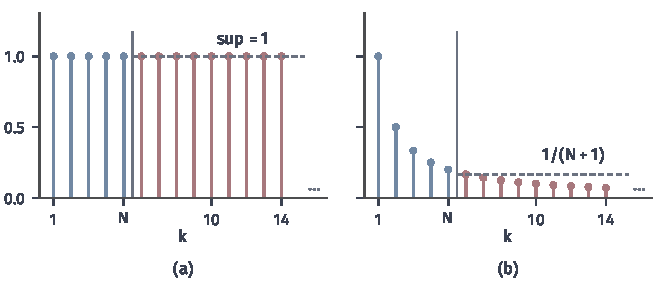
\includegraphics[width=112mm]{figures/04-spaces-measures-and-geometry/03-function-spaces/matplotlib/fvec-truncation-error/figure.pdf}
  \caption{同样的截断，不同的尾部。这里$N=5$，竖线左侧蓝色为保留的项，右侧红色为截掉的项，也就是误差，虚线标出误差的上确界。(a)常数列的尾部一直保持高度$1$，$N$增大时只是整体右移。(b)调和数列的尾部越来越低，上确界为$1/(N+1)$，随$N$增大而趋于零。}
  \label{fig:fvec-truncation-error}
\end{BookInlineFigure}

\paragraph{收敛意义的选择}
两个级数形式完全相同，都是$\sum_kx_ke_k$，区别只在系数。表~\ref{tab:fvec-truncation-compare}对比了两种误差给出的结论。在逐项收敛的意义下，每个数列都能这样展开；在统一误差的意义下，只有尾部趋于零的数列才能这样展开，也就是恰好$c_0$中的数列。所以“级数收敛”本身不是一个完整的陈述，必须说明用哪种误差衡量。

\begin{BookInlineTable}
  \centering
  \begin{tabular}{@{}lll@{}}
    \toprule
    误差的衡量方式 & $x=(1,1,1,\ldots)$ & $y=(1,\tfrac12,\tfrac13,\ldots)$\\
    \midrule
    逐项 & 收敛 & 收敛\\
    所有项的上确界 & 恒等于$1$，不收敛 & $1/(N+1)$，收敛\\
    \bottomrule
  \end{tabular}
  \caption{同一种截断在两种误差下的结论。}
  \label{tab:fvec-truncation-compare}
\end{BookInlineTable}

函数的情形相同，系数列$[1,1,\tfrac12,\tfrac16,\ldots]$就是一个例子。$e^x$的部分和是
\[
 s_N(x)=\sum_{k=0}^N\frac{x^k}{k!}.
\]
先在$[0,1]$上看误差。对$0\leq x\leq1$，把每个$x^k$放大到$1$，得到
\[
 0\leq e^x-s_N(x)=\sum_{k\geq N+1}\frac{x^k}{k!}\leq\sum_{k\geq N+1}\frac1{k!}.
\]

右边从$k=N+1$起，每一项不超过前一项的一半，所以用等比级数控制它：
\begin{equation}
 \sup_{0\leq x\leq1}\lvert e^x-s_N(x)\rvert\leq\frac{2}{(N+1)!}.
 \label{eq:fvec-exp-truncation}
\end{equation}
取$N=3$时，这个上界是$\tfrac1{12}$。所以在$[0,1]$上，统一误差趋于零。

换到整条实轴，结论就变了。在每个固定的$x$处，$s_N(x)$仍趋于$e^x$，因为这个幂级数处处收敛。但固定$N$后，对$x>0$有
\[
 e^x-s_N(x)\geq\frac{x^{N+1}}{(N+1)!},
\]
右边随$x\to+\infty$趋于无穷。所以每个$N$的统一误差都是无穷大，同一个级数在$\mathbb R$上逐点收敛、不一致收敛。

对一列近似函数，可以要求每个输入处的值收敛（逐点收敛），可以要求所有输入上的最大误差趋于零（一致收敛），也可以要求误差的积分趋于零。这三种意义互不等价。第~\ref{chap:function-normed-spaces}章用范数统一表达整体误差并比较这些收敛方式，具体表示及其截断误差则在第~\ref{chap:function-inner-product-spaces}章的正交展开和第~\ref{chap:function-approximation}章的函数逼近中研究。

\section{无限维闭球不紧}
\label{sec:fvec-closed-ball-noncompact}

在$\mathbb R^d$中，有界序列总有收敛子列，闭有界集上的连续函数总取到最小值。许多存在性论证都是这样进行的：先找一列越来越好的近似，再从中抽出收敛子列，最后说明极限就是所求的对象。本节说明，这条路在无限维空间中会断。

标准单位列已经显示了问题所在。在$c_0$中用各项之差的上确界作距离，$e_m$与$e_n$（$m\neq n$）在第$m$项相差$1$，其余各项相差不超过$1$，所以二者的距离恰为$1$。这些点都在以零数列为中心、半径为$1$的闭球里，它们彼此隔开，没有任何子列收敛。

本节要证明这不是$c_0$的特殊现象，而是所有无限维赋范空间的共同性质。这里需要用距离衡量“彼此隔开”，所以先回顾卷二的范数。线性空间$V$上的范数$\lVert\cdot\rVert$是满足正定性、齐次性$\lVert cx\rVert=\lvert c\rvert\lVert x\rVert$与三角不等式的非负函数，它诱导距离$d(x,y)=\lVert x-y\rVert$；配有范数的空间称为赋范空间。

有限维情形的范数理论可参考\BookChapterRef{chap:normed-spaces}{卷二第3章“赋范空间”}，无限维的系统讨论在第~\ref{chap:function-normed-spaces}章。本节只用这些公理和距离的语言。

\paragraph{有限维子空间是闭集}
下面的构造要用到这样一个事实：在任意赋范空间中，有限维子空间是闭集。平面上过原点的直线、三维空间中过原点的平面都是闭集，无限维的环境空间里这一点仍然成立。

\begin{lemma}[有限维子空间闭性]
\label{lem:fvec-finite-subspace-closed}
设$X$是赋范空间，$Y\subseteq X$是有限维线性子空间。则$Y$是$X$中的闭集。
\end{lemma}

\begin{proof}
设$y_n\in Y$且在$X$中$y_n\to x$，要证$x\in Y$。收敛序列是柯西列，所以$\{y_n\}$是$Y$中的柯西列。

把$X$的范数限制在$Y$上，$Y$成为一个有限维赋范空间。卷二证明了有限维赋范空间在任意范数下都完备，所以$\{y_n\}$在$Y$中收敛到某个$y$。

这个$y$也是$\{y_n\}$在$X$中的极限。第~\ref{chap:metric-spaces}章说明度量空间中的极限唯一，所以$x=y\in Y$。
\end{proof}

这个论证没有要求$X$完备，只用到$Y$自身的完备性。由闭性，若$x_0\notin Y$，则$x_0$到$Y$的距离
\[
 d(x_0,Y)=\inf_{y\in Y}\lVert x_0-y\rVert
\]
严格为正：否则可在$Y$中取一列$y_n$使$\lVert x_0-y_n\rVert\to0$，闭性给出$x_0\in Y$，矛盾。

\paragraph{Riesz引理}
要在无限维空间中造出彼此远离的单位向量，先看$\mathbb R^2$中是怎样做的。取一条过原点的直线$Y$和线外一点$x_0$，从$x_0$向$Y$作垂线，垂足是$Y$上离$x_0$最近的点。$x_0$减去垂足再归一化，就得到与$Y$垂直的单位向量，它到$Y$的距离恰为$1$。

一般赋范空间没有垂直，$Y$上的最近点也可能不存在，所以要退一步：不取最近点，而取一个几乎最近的点$y_0$。图~\ref{fig:fvec-riesz-lemma}画出了这个做法。$x_0-y_0$不再与$Y$垂直，归一化后的向量$x$略微倾斜，但它到$Y$的距离仍接近$1$。

\begin{BookInlineFigure}
  \centering
  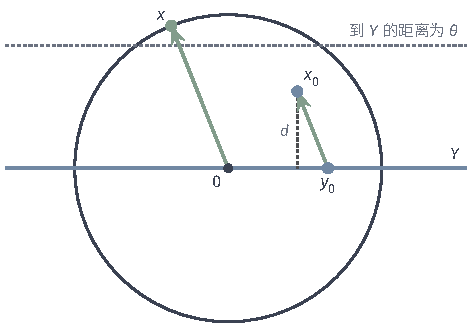
\includegraphics[width=79.904mm]{figures/04-spaces-measures-and-geometry/03-function-spaces/tikz/fvec-riesz-lemma/figure.pdf}
  \caption{Riesz引理的构造在$\mathbb R^2$中的样子。蓝色直线是子空间$Y$，圆是单位球面。$x_0$到$Y$的距离为$d$，$y_0$是$Y$上一个几乎最近的点。把向量$x_0-y_0$（绿色）平移到原点并归一化，得到单位向量$x$，它落在虚线上方，到$Y$的距离不小于$\theta$。}
  \label{fig:fvec-riesz-lemma}
\end{BookInlineFigure}

把这个几何过程写成不等式，就得到下面的引理。

\begin{lemma}[Riesz引理]
\label{lem:fvec-riesz}
设$X$是赋范空间，$Y\subsetneq X$是闭线性子空间，$0<\theta<1$。则存在$x\in X$，使$\lVert x\rVert=1$，并且
\begin{equation}
 \lVert x-y\rVert\geq\theta,\qquad y\in Y.
 \label{eq:fvec-riesz}
\end{equation}
\end{lemma}

\begin{proof}
取$x_0\in X\setminus Y$，记$d=d(x_0,Y)$。由$Y$闭，$d>0$。因为$d/\theta>d$，由下确界的定义可以取$y_0\in Y$使
\[
 d\leq\lVert x_0-y_0\rVert\leq\frac{d}{\theta}.
\]
令$c=\lVert x_0-y_0\rVert$，并取$x=(x_0-y_0)/c$，则$\lVert x\rVert=1$。

对任意$y\in Y$，把$x-y$通分，写成
\[
 x-y=\frac{x_0-(y_0+cy)}{c}.
\]
括号里的$y_0+cy$仍属于线性子空间$Y$，所以分子的范数至少是$d$。于是
\[
 \lVert x-y\rVert\geq\frac{d}{c}\geq\frac{d}{d/\theta}=\theta.
\]
\end{proof}

引理的两个条件都不能去掉。先看“$Y$闭”。在$c_0$中取$Y=c_{00}$，它是真子空间，但不闭。对任意$x\in c_0$，截断$s_N$属于$Y$，并且
\[
 \sup_{k\geq1}\lvert x_k-(s_N)_k\rvert=\sup_{k>N}\lvert x_k\rvert\to0,
\]
所以每个$x$到$Y$的距离都是$0$，式~\eqref{eq:fvec-riesz}对任何$\theta>0$都不成立。

再看$\theta<1$。在有限维中$\theta=1$可以取到，因为最近点存在；无限维中最近点可能取不到，$\theta=1$就可能失败。下面是一个能手算的例子。

\begin{example}[$\theta=1$可能失败]
\label{ex:fvec-riesz-theta-one}
令$X=\{f\in C[0,1]:f(0)=0\}$，范数取$\lVert f\rVert=\max_t\lvert f(t)\rvert$，令
\[
 Y=\Bigl\{f\in X:\int_0^1f(t)\,dt=0\Bigr\}.
\]
$Y$是闭子空间，因为$\lvert\int f-\int g\rvert\leq\lVert f-g\rVert$，积分为零的性质在一致极限下保持。

任取$X$中的单位向量$x$，构造$Y$中逼近它的元素。令$h_n(t)=\min(nt,1)$，则$h_n\in X$，$\lVert h_n\rVert=1$，并且积分为
\[
 \int_0^1h_n(t)\,dt=1-\frac1{2n}.
\]
记$I=\int_0^1x(t)\,dt$，令
\[
 y_n=x-\frac{I}{1-\frac1{2n}}h_n,
\]
它的积分为$I-I=0$，所以$y_n\in Y$。

$x$到$y_n$的距离由$h_n$的系数给出：
\[
 \lVert x-y_n\rVert=\frac{\lvert I\rvert}{1-\frac1{2n}}.
\]
令$n\to\infty$，得到$d(x,Y)\leq\lvert I\rvert$。而$x$连续且$x(0)=0$，所以在$0$附近$\lvert x\rvert<\tfrac12$，又处处有$\lvert x\rvert\leq1$，于是$\lvert I\rvert<1$。

所以$X$中每个单位向量到$Y$的距离都严格小于$1$，$\theta=1$的结论不成立。
\end{example}

\paragraph{两两远离的单位向量}
现在设$X$是无限维赋范空间，用Riesz引理逐个构造单位向量。任取一个单位向量$e_1$。设已经得到单位向量$e_1,\ldots,e_n$，令
\[
 Y_n=\operatorname{span}\{e_1,\ldots,e_n\}.
\]
$Y_n$是有限维子空间，由引理~\ref{lem:fvec-finite-subspace-closed}是闭集；$X$无限维，所以$Y_n\neq X$。对$Y_n$与$\theta=\tfrac12$应用引理~\ref{lem:fvec-riesz}，得到单位向量$e_{n+1}$，它到$Y_n$中每一点的距离都至少为$\tfrac12$。

这样得到的序列$\{e_n\}$有两条性质。其一，它线性无关：$e_{n+1}$到$Y_n$的距离为正，所以$e_{n+1}\notin Y_n$，每个新元素都不能由之前的元素线性表示。其二，它两两远离：对$m<n$，$e_m\in Y_{n-1}$，所以
\begin{equation}
 \lVert e_n-e_m\rVert\geq\frac12,\qquad m\neq n.
 \label{eq:fvec-separated-sequence}
\end{equation}
第~\ref{chap:function-normed-spaces}章构造不等价范数时，还会用到这里的单位列$\{e_n\}$。

有了这列向量，闭球不紧的结论就只差一步。

\begin{theorem}[无限维闭球不紧]
\label{thm:fvec-closed-ball-noncompact}
设$X$是无限维赋范空间。则闭单位球$\bar B=\{x\in X:\lVert x\rVert\leq1\}$不是全有界的，从而不紧。更一般地，对任意$a\in X$与$r>0$，闭球$\{x:\lVert x-a\rVert\leq r\}$都不紧。
\end{theorem}

\begin{proof}
全有界要求对每个$\varepsilon>0$，$\bar B$都能被有限个半径为$\varepsilon$的开球覆盖。取$\varepsilon=\tfrac14$。半径$\tfrac14$的开球中任意两点的距离小于$\tfrac12$，由式~\eqref{eq:fvec-separated-sequence}，每个这样的球至多含有一个$e_n$。$\bar B$中有无穷多个$e_n$，有限个球盖不住它们，所以$\bar B$不全有界。第~\ref{chap:metric-spaces}章证明了紧度量空间必定全有界，故$\bar B$不紧。

也可以直接从序列看：$\{e_n\}$的任何子列都满足式~\eqref{eq:fvec-separated-sequence}，不是柯西列，因而不收敛。

对一般的闭球，映射$x\mapsto a+rx$把$\bar B$一一地映成该闭球，并把距离乘以$r$。若该闭球紧，则$a+re_n$有收敛子列，相应的$e_n$子列也收敛，矛盾。
\end{proof}

证明从头到尾没有用到$X$的完备性。不紧的原因不是“缺少极限点”，而是有界的区域里装得下无穷多个互相隔开的点。

有限维中这样的点只能有有限个，用体积就能数出来。设$\mathbb R^d$的单位球中有$N$个点两两距离至少为$\tfrac12$。以这些点为中心、半径$\tfrac14$的开球两两不交，并且都含在半径$\tfrac54$的球内。比较体积，得到
\[
 N\Bigl(\frac14\Bigr)^d\leq\Bigl(\frac54\Bigr)^d.
\]
约去公因子，就是
\begin{equation}
 N\leq5^d.
 \label{eq:fvec-packing-bound}
\end{equation}
所以$\mathbb R^2$的单位圆盘中至多有$25$个这样的点。这个上界随$d$增大而迅速增大，$d$无限时不再有任何上界，这就是无限维中闭球不紧的直观原因。图~\ref{fig:fvec-bounded-noncompact}(a)是$d=2$的情形。

\paragraph{连续函数的例子}
Riesz引理给出的是存在性。在具体的函数空间中，往往可以直接写出没有收敛子列的有界序列。考虑$C[0,1]$，以两个函数之差的最大绝对值
\[
 d(f,g)=\max_{x\in[0,1]}\lvert f(x)-g(x)\rvert
\]
为距离。连续函数在闭区间上取到最大值，所以$d$有定义；它来自范数$\max_x\lvert f(x)\rvert$，按这一距离收敛就是一致收敛。

\begin{BookInlineFigure}
  \centering
  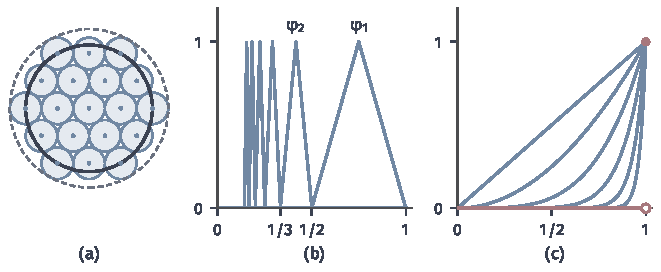
\includegraphics[width=112mm]{figures/04-spaces-measures-and-geometry/03-function-spaces/matplotlib/fvec-bounded-noncompact/figure.pdf}
  \caption{有界而不紧。(a)$\mathbb R^2$单位圆盘（实线）内的$19$个点，两两距离不小于$\tfrac12$，半径$\tfrac14$的小圆盘互不重叠，全部落在半径$\tfrac54$的虚线圆内。(b)在$C[0,1]$中，前六个鼓包$\varphi_n$的支撑互不重叠，高度都是$1$。(c)蓝色为$x^n$（$n=1,2,4,8,16,32$），红色为逐点极限：$[0,1)$上为$0$，在$1$处取$1$。}
  \label{fig:fvec-bounded-noncompact}
\end{BookInlineFigure}

最接近标准单位列的是一列鼓包。对$n\geq1$，令$\varphi_n$在区间$[\tfrac1{n+1},\tfrac1n]$的中点取$1$，在区间两端取$0$，在区间上线性插值，在区间外恒为$0$。图~\ref{fig:fvec-bounded-noncompact}(b)显示，这些鼓包各占一段位置，相当于各占一个“坐标”。

当$m\neq n$时，$\varphi_m$与$\varphi_n$的支撑至多在一点相接，而两函数在该点都为零，所以每点至多有一个函数非零。在$\varphi_n$的峰值点，差的绝对值为$1$，于是
\[
 d(\varphi_m,\varphi_n)=1,\qquad m\neq n.
\]
它们都在以零函数为中心、半径为$1$的闭球内，没有任何子列收敛。

再看$f_n(x)=x^n$，它的表现不同。每个$f_n$满足$0\leq x^n\leq1$，所以也都在同一个闭球内。相邻两项的差$x^n(1-x)$在$x=\tfrac n{n+1}$处取最大值，由此
\[
 d(f_n,f_{n+1})=\Bigl(\frac n{n+1}\Bigr)^n\frac1{n+1}\leq\frac1{n+1},
\]
相邻两项越来越近。序列看上去在收敛，但它仍然没有任何按$d$收敛的子列。

设子列$f_{n_k}$按$d$收敛到某个$g\in C[0,1]$。一致收敛推出逐点收敛，所以对每个$x$，$g(x)=\lim_kx^{n_k}$。当$0\leq x<1$时这个极限是$0$，当$x=1$时是$1$。于是$g$在$[0,1)$上恒为$0$而$g(1)=1$，在$1$处不连续，与$g\in C[0,1]$矛盾。

两个例子失败的方式不同。鼓包的逐点极限是零函数，它就在$C[0,1]$中，可是每个鼓包离它的距离总是$1$，逐点接近不等于一致接近。$x^n$的逐点极限跑出了$C[0,1]$，候选极限根本不在空间里。函数类在什么附加条件下恢复紧性，例如要求一致有界并且等度连续，是第~\ref{chap:metric-space-maps}章和第~\ref{chap:function-class-covers}章的内容。

\section{本章小结}
\label{sec:fvec-summary}

本章开头的问题是：把函数看作向量$[\ldots,f(x),\ldots]$时，有限维线性代数的语言保留了什么，又在哪里失效。表~\ref{tab:fvec-summary}按本章的顺序汇总了答案。

\begin{BookInlineTable}
  \centering
  \begin{tabular}{@{}p{18mm}p{36mm}p{48mm}@{}}
    \toprule
    概念 & 有限维向量 & 无限维函数空间\\
    \midrule
    线性运算 & 逐分量计算 & 逐点计算，规则相同\\
    维数 & 分量个数 & 与输入点数无关，要看函数集合\\
    取值与坐标 & 标准基下坐标就是分量 & 取值一般不是有限组合的坐标\\
    基 & 有限个，有限组合表示全部 & 代数基只允许有限组合，通常写不出\\
    无穷和 & 用不到 & 收敛、范围、唯一性都依赖误差\\
    逐分量与统一误差 & 两种收敛等价 & 两种收敛不同\\
    有界序列 & 总有收敛子列 & 可以没有收敛子列\\
    \bottomrule
  \end{tabular}
  \caption{有限维向量的语言在无限维函数空间中的保留与失效。}
  \label{tab:fvec-summary}
\end{BookInlineTable}

线性运算的部分完整地保留下来。逐点加法与数乘使全体函数$X\to\mathbb K$成为线性空间，数列与有限维向量都是它的特例。连续函数、限次多项式、收敛到零的数列和有限支撑数列都通过了子空间核验。函数作为元素、它在某点的值、它相对于某组基的坐标是三样不同的东西；乘法和求导也不是每个函数空间自带的运算。

维数仍按张成整个空间需要多少方向来计算，与定义域的点数无关。有限输入集合上的函数以指示函数为基，坐标就是函数值。$P_m$定义在整条实轴上，却只有$m+1$维，取值列与系数列由一个可逆矩阵互相决定。全体多项式、全体数列含有任意多个线性无关的元素，因而是无限维的。其中每个元素可能只用到有限个方向，但没有一组固定的有限方向能表示所有元素。

无限维带来两个困难。其一，代数基只允许有限组合，要表示常数列或$e^x$这样的元素就须借助级数，而级数是否收敛、能表示哪些元素、系数是否唯一，都取决于选用的误差。其二，任何无限维赋范空间中，Riesz引理都给出两两距离至少$\tfrac12$的单位向量列，所以正半径闭球都不紧，这一结论不需要空间完备。

这两个困难分别指向后面两章。第~\ref{chap:function-normed-spaces}章用范数规定整体误差，比较不同范数下的收敛，并用完备性保证柯西列的极限留在空间内；第~\ref{chap:function-inner-product-spaces}章再加入内积，用正交投影和正交展开给出收敛的无限表示。闭球不紧则提醒我们：在无限维中求极值或抽收敛子列，需要额外的紧性条件或更弱的收敛概念。


\chapter{赋范空间}
\label{chap:normed-spaces}
\label{chap:functional-analysis-and-approximation}

用$x^2$近似$[0,1]$上的$x$，误差有多大？若关心最坏的位置，可以取$\max_x\lvert x-x^2\rvert=\tfrac14$；若关心整体的累计偏差，可以取$\int_0^1\lvert x-x^2\rvert\,dx=\tfrac16$。两个数都合理，回答的是不同的问题。一列近似函数是否收敛，也要先说清用哪一种误差。上一章把函数当作向量，却还没有规定函数之间的距离；本章用范数做这件事，并研究不同范数下的收敛与极限。

第~\ref{sec:nspace-norms}节把卷二的范数公理用于整个函数，说明范数怎样给出收敛与柯西列，并借助上一章两两远离的单位列说明：无限维空间上总可以构造不等价的范数，同一列函数在一种范数下收敛、在另一种下可能不收敛。范数选定以后，还要问柯西列的极限是否仍在空间内，这是第~\ref{sec:nspace-banach-spaces}节的完备性。

随后三节给出具体的完备空间。第~\ref{sec:nspace-continuous-function-spaces}节证明紧集上的连续函数在最大误差下完备，而同一个集合在积分误差下不完备。为了给积分误差下的极限找到去处，第~\ref{sec:nspace-lp-spaces}节和第~\ref{sec:nspace-linfty-space}节在可测函数的几乎处处等价类上建立$L^p$与$L^\infty$，证明Hölder与Minkowski不等式和完备性。最后，第~\ref{sec:nspace-convergence-of-sequences}节比较逐点、一致、$L^p$及依测度收敛分别控制什么误差，并用一致可积性说明何时可以从依测度收敛得到积分收敛。

本章所用的测度与积分来自第~\ref{chap:measure}章和第~\ref{chap:integration}章，度量空间中的收敛、柯西列与完备性来自第~\ref{chap:metric-spaces}章，映射列的一致收敛来自第~\ref{chap:metric-space-maps}章。内积带来的正交结构在第~\ref{chap:inner-product-spaces}章研究；空间之间的包含映射作为有界算子在第~\ref{chap:linear-operators}章研究；简单函数、连续函数在$L^p$中的稠密性等逼近问题在第~\ref{chap:function-approximation}章研究。

\section{范数}
\label{sec:nspace-norms}

要判断两个函数整体上是否接近，先要给它们的差$f-g$规定一个“大小”，再用这个大小是否趋于零来判断近似是否成功。卷二已经用范数公理规定了向量的大小，本节把这套公理用到整个函数上。先说明函数范数的含义，再说明它给出的收敛与柯西列，最后说明无限维空间中不同范数之间可能无法互相控制。

\subsection{函数的范数}
\label{sec:nspace-function-norms}

函数的范数衡量的是整个函数的大小，而不是某一点处的函数值。要让不同的大小规则共享同一套推理，只要求它们满足几条共同的性质，这就是卷二的范数公理。

\begin{definition}[范数与赋范空间]
\label{def:nspace-norm}
设$V$是$\mathbb K$上的线性空间。映射$\lVert\cdot\rVert:V\to[0,\infty)$称为$V$上的\term{范数}（norm），若对所有$f,g\in V$与$c\in\mathbb K$：
\begin{enumerate}
 \item 正定性：$\lVert f\rVert=0$当且仅当$f=0$；
 \item 齐次性：$\lVert cf\rVert=\lvert c\rvert\,\lVert f\rVert$；
 \item 三角不等式：$\lVert f+g\rVert\leq\lVert f\rVert+\lVert g\rVert$。
\end{enumerate}
配备范数的线性空间$(V,\lVert\cdot\rVert)$称为\term{赋范空间}（normed space）。
\end{definition}

对函数而言，正定性中的“$f=0$”指$f$是零元素。在逐点运算的函数空间里，零元素是处处为零的函数，所以$\lVert f\rVert=0$必须迫使$f$在每一点都为零。齐次性说明把函数整体放大$c$倍，大小也放大$\lvert c\rvert$倍。三角不等式说明两段误差串联起来不超过各自之和，它是后面误差估计的基本工具。有限维范数的例子与性质，可参考\BookChapterRef{chap:normed-inner-product-spaces}{卷二第3章“赋范空间与内积空间”}。

\paragraph{两种整体大小}
在$C[0,1]$上，最常用的两种大小是
\[
 \lVert f\rVert_\infty=\max_{x\in[0,1]}\lvert f(x)\rvert,\qquad \lVert f\rVert_1=\int_0^1\lvert f(x)\rvert\,dx.
\]
前者看最坏的位置，后者看绝对值曲线下的总面积。对$h(x)=x-x^2$，$\lVert h\rVert_\infty=\tfrac14$，$\lVert h\rVert_1=\tfrac16$，这就是章首的两个数。两者都不是函数在某一点的值：$h(0)=0$，但$h$并不是零元素。

逐条核对公理。$\lVert\cdot\rVert_\infty$的齐次性和三角不等式在每个$x$处成立后取最大值即得；若最大值为$0$，则每点$\lvert f(x)\rvert=0$。$\lVert\cdot\rVert_1$的齐次性与三角不等式来自积分的线性与单调性。正定性需要连续：若$f$在某点$x_0$处$\lvert f(x_0)\rvert=a>0$，则在$x_0$附近的一个区间上$\lvert f\rvert>a/2$，积分为正。

\paragraph{有限性与正定性要逐个空间核验}
同一个公式放到别的函数集合上，公理可能不再成立。把$\int_0^1\lvert f\rvert$用于$[0,1]$上的有界黎曼可积函数，正定性失效：只在$x=\tfrac12$处取$1$、其余处取$0$的函数不是零函数，积分却为$0$。这样只满足齐次性与三角不等式、允许非零元素大小为零的函数称为\term{半范数}（seminorm）。

公式的值也可能是无穷。把$\max\lvert f\rvert$换成$\sup\lvert f\rvert$用于$\mathbb R$上的连续函数，$f(x)=x$的上确界为$+\infty$，不是实数。所以给一个函数集合配范数时，要分别核验三件事：集合对线性运算封闭，公式对集合中每个元素有限，正定性在这个集合上成立。第~\ref{sec:nspace-continuous-function-spaces}节到第~\ref{sec:nspace-linfty-space}节对各个具体空间逐一完成这些核验，其中积分范数的正定性要靠把几乎处处相等的函数看作同一个元素来恢复。

\subsection{范数与收敛}
\label{sec:nspace-norm-convergence}

范数给出距离$d(f,g)=\lVert f-g\rVert$。由三条公理可以直接验证距离公理，例如三角不等式$d(f,h)=\lVert(f-g)+(g-h)\rVert\leq d(f,g)+d(g,h)$。所以每个赋范空间都是度量空间，第~\ref{chap:metric-spaces}章关于点列收敛、柯西列、闭集和完备性的结论都可以直接使用。

\paragraph{依范数收敛与柯西列}
按这个距离，序列$(f_n)$收敛到$f$就是$\lVert f_n-f\rVert\to0$，称为\term{依范数收敛}（convergence in norm）。$(f_n)$是柯西列，就是对每个$\varepsilon>0$存在$N$，使$m,n\geq N$时$\lVert f_n-f_m\rVert<\varepsilon$。收敛列都是柯西列；反过来是否成立取决于空间，这是下一节的问题。

范数的选择决定了收敛控制什么。在$C[0,1]$上，$\lVert f_n-f\rVert_\infty\to0$说明对每个$\varepsilon>0$，从某个$N$起，所有输入处的误差同时不超过$\varepsilon$，这正是一致收敛。$\lVert f_n-f\rVert_1\to0$只说明误差曲线下的面积趋于零，允许在越来越窄的区间上保留较大的误差。由$\lVert h\rVert_1\leq\lVert h\rVert_\infty$，一致收敛推出积分误差收敛；下一小节将说明反过来不成立。

\paragraph{等价范数}
若同一空间上的两个范数能互相控制，它们给出的收敛判断就完全一致。

\begin{definition}[等价范数]
\label{def:nspace-equivalent-norms}
线性空间$V$上的两个范数$N_1,N_2$称为\term{等价范数}（equivalent norms），若存在常数$0<c\leq C$，使对所有$f\in V$，
\[
 c\,N_1(f)\leq N_2(f)\leq C\,N_1(f).
\]
\end{definition}

对$h=f_n-f$使用右边的不等式，$N_1(f_n-f)\to0$推出$N_2(f_n-f)\to0$；左边的不等式给出反方向。对$h=f_n-f_m$使用同样的不等式，两个范数下的柯西列也相同。所以等价范数给出相同的收敛序列、相同的极限和相同的柯西列，完备性也随之相同。关键是常数$c,C$与$f$无关。

有限维空间中，任意两个范数都等价，卷二已经证明了这一点。因此有限维空间的收敛与完备性不依赖范数的选择，只有误差的具体数值与常数随范数改变。卷二的证明用到有限维单位球面的紧性，上一章说明这一性质在无限维中失效，所以无限维空间中的两个范数是否等价，需要另作判断。

\subsection{范数不等价}
\label{sec:nspace-inequivalent-norms}

下面先从一般的无限维赋范空间出发，构造一个与原范数不等价的新范数，再在$C[0,1]$上给出一对具体的不等价范数。

\paragraph{用代数基构造}
设$(X,N_1)$是无限维赋范空间，$\{e_n\}_{n\geq1}$是第~\ref{chap:functions-as-vectors}章用Riesz引理构造的单位列：$N_1(e_n)=1$，且$\{e_n\}$线性无关。用选择公理可以把这个线性无关族扩充为$X$的一组代数基$B\supseteq\{e_n\}$，这里不给出证明。每个$x\in X$都唯一地写成$B$中有限个元素的组合。

在基上规定$Te_n=e_n/n$，对其余的$b\in B$规定$Tb=b$，再线性延拓：对$x=\sum_{b}c_bb$（有限和），令$Tx=\sum_bc_b\lambda_bb$，其中$\lambda_{e_n}=1/n$，其余$\lambda_b=1$。表示唯一，所以$T$是定义合理的线性映射。$T$还是单射：若$Tx=0$，由表示的唯一性，每个$c_b\lambda_b=0$，而$\lambda_b\neq0$，故每个$c_b=0$。

令$N_2(x)=N_1(Tx)$。它是范数：齐次性与三角不等式由$T$的线性和$N_1$的相应性质得到，例如$N_2(x+y)=N_1(Tx+Ty)\leq N_2(x)+N_2(y)$；若$N_2(x)=0$，则$Tx=0$，由单射得$x=0$。但
\[
 N_1(e_n)=1,\qquad N_2(e_n)=N_1(e_n/n)=\frac1n.
\]
若存在$c>0$使$cN_1\leq N_2$，取$x=e_n$得$c\leq1/n$对所有$n$成立，矛盾。所以$N_1$与$N_2$不等价：序列$e_n$在$N_2$下趋于零，在$N_1$下却始终与零相距$1$。

这个构造说明，每个无限维赋范空间上都存在与原范数不等价的范数。它是纯粹的存在性论证：代数基无法具体写出，$N_2$也就无法具体计算。

\paragraph{连续函数上的一对具体范数}
在$C[0,1]$上，$\lVert\cdot\rVert_\infty$与$\lVert\cdot\rVert_1$就不等价。一个方向的控制成立：$\lvert f(x)\rvert\leq\lVert f\rVert_\infty$对每个$x$成立，在$[0,1]$上积分得$\lVert f\rVert_1\leq\lVert f\rVert_\infty$。另一个方向没有常数：取$f_n(x)=x^n$，
\[
 \lVert x^n\rVert_\infty=1,\qquad \lVert x^n\rVert_1=\int_0^1x^n\,dx=\frac1{n+1}\to0.
\]
若$\lVert f\rVert_\infty\leq C\lVert f\rVert_1$，则$1\leq C/(n+1)$对所有$n$成立，矛盾。

图~\ref{fig:nspace-xn-norms}显示了这一差别的来源。$x^n$只在靠近$1$的越来越窄的区间上取较大的值，积分看到的是这段区间的面积，最大值看到的是峰顶。同一列函数在积分范数下趋于零函数，在最大值范数下与零函数的距离始终为$1$。图中的平方积分大小$\lVert x^n\rVert_2=(2n+1)^{-1/2}$在第~\ref{sec:nspace-lp-spaces}节正式定义。

\begin{figure}[!htb]
  \centering
  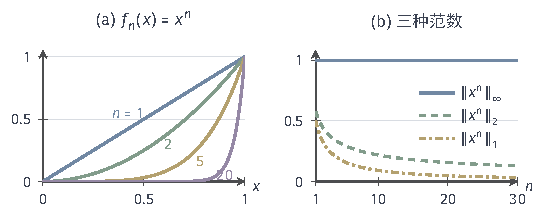
\includegraphics[width=92.3mm]{figures/02-abstract-mathematics/03-function-spaces/tikz/c1-xn-norms/figure.pdf}
  \caption{$x^n$在$[0,1]$上的三种大小。(a)$n=1,2,5,20$时的曲线，较大的函数值集中到右端越来越窄的区间上。(b)三种大小随$n$的变化：$\lVert x^n\rVert_\infty=1$保持不变，$\lVert x^n\rVert_2=(2n+1)^{-1/2}$与$\lVert x^n\rVert_1=(n+1)^{-1}$趋于零。}
  \label{fig:nspace-xn-norms}
\end{figure}

\paragraph{与有限维的对照}
卷二的结论是“有限维空间中任意两个范数都等价”。它在无限维中的否定是“存在不等价的范数”，而不是“任意两个范数都不等价”。例如$\lVert\cdot\rVert_\infty$与$2\lVert\cdot\rVert_\infty$在任何空间上都等价，常数为$c=C=2$。

因此在无限维空间中谈论收敛，必须同时说明用哪个范数。说“$x^n$在$C[0,1]$中收敛到$0$”是不完整的陈述：在$\lVert\cdot\rVert_1$下它成立，在$\lVert\cdot\rVert_\infty$下它不成立。后面各节始终把空间与范数一起给出。

\section{Banach空间}
\label{sec:nspace-banach-spaces}

迭代算法、级数截断和逐步加细的逼近，常常只告诉我们近似之间越来越接近，即得到一个柯西列，而不直接给出极限。要从“彼此接近”推出“存在极限”，空间里必须真有这个极限。范数规定了怎样衡量接近，却不保证这一点；后者是空间与范数共同的性质。

\begin{definition}[Banach空间]
\label{def:nspace-banach}
若赋范空间$V$中的每个柯西列都依范数收敛到$V$中的某个元素，即范数诱导的度量空间是完备的，称$V$是\term{完备}（complete）的赋范空间，也称\term{Banach空间}（Banach space）。
\end{definition}

这就是第~\ref{chap:metric-spaces}章的完备性，只是度量来自范数。卷二已经证明有限维赋范空间在任意范数下都完备，所以有限维时无需另作核验。无限维时，完备与否要逐个空间证明；同一个集合换一个范数，结论可能改变，第~\ref{sec:nspace-continuous-function-spaces}节会给出这样的例子。

\paragraph{闭子空间判据}
很多函数空间是另一个已知完备空间的子空间。这时可以借用第~\ref{chap:metric-spaces}章的两个结论：完备度量空间中的闭子集是完备的；任何度量空间中的完备子集都是闭集。用在Banach空间$X$的线性子空间$M$上，就得到下面的判据。

\begin{theorem}[闭子空间判据]
\label{thm:nspace-closed-subspace}
设$X$是Banach空间，$M\subseteq X$是线性子空间，$M$带有限制后的范数。则$M$是Banach空间当且仅当$M$是$X$中的闭集。
\end{theorem}

\begin{proof}
设$M$闭，$(f_n)$是$M$中的柯西列。它也是$X$中的柯西列，由$X$完备收敛到某个$f\in X$；$M$闭，所以$f\in M$。反过来，设$M$完备，$f_n\in M$且在$X$中$f_n\to f$。收敛列是柯西列，所以$(f_n)$是$M$中的柯西列，在$M$中收敛到某个$g$；$X$中极限唯一，$f=g\in M$，所以$M$闭。
\end{proof}

两个方向的分工不同。从闭推出完备时，大空间$X$的完备性提供极限，$M$的闭性保证极限没有离开$M$。从完备推出闭时，并不需要$X$完备，第~\ref{chap:functions-as-vectors}章证明有限维子空间闭性时用的正是这一方向。

\paragraph{不闭的子空间}
多项式给出一个不完备的例子。在$[0,1]$上用$\lVert f\rVert_\infty=\max_x\lvert f(x)\rvert$衡量多项式，取$e^x$的Taylor多项式$p_N(x)=\sum_{k=0}^Nx^k/k!$。由Lagrange余项，
\[
 \max_{x\in[0,1]}\lvert e^x-p_N(x)\rvert\leq\frac{e}{(N+1)!}\to0,
\]
所以对$m>n$，$\lVert p_m-p_n\rVert_\infty\leq\frac{e}{(m+1)!}+\frac{e}{(n+1)!}$，$(p_N)$是多项式空间中的柯西列。

它在多项式空间中没有极限。若有多项式$p$使$\lVert p_N-p\rVert_\infty\to0$，则对每个$x$都有$p_N(x)\to p(x)$；又$p_N(x)\to e^x$，所以$p=e^x$在$[0,1]$上成立。但多项式求足够多次导数后恒为零，$e^x$的各阶导数都不为零，矛盾。所以多项式空间在最大误差下不完备；下一节证明$C[0,1]$完备后，闭子空间判据说明这等价于多项式空间在$C[0,1]$中不闭。

\paragraph{范数与完备性是两个问题}
给一个函数集合配范数，回答的是“怎样衡量误差”；问它是否完备，回答的是“误差趋零的过程能否在集合内找到终点”。前者只要核验三条公理，后者要分析柯西列的极限。不完备的赋范空间仍然是合法的赋范空间，只是不能仅凭柯西性断言极限存在。

不完备的空间可以通过补入极限变成完备的：第~\ref{chap:metric-spaces}章的完备化构造对赋范空间同样适用，线性运算和范数都可以沿柯西列延拓。但抽象完备化只保证新元素存在，不说明它们是哪一类函数。本章采用另一条路：直接在更大的函数集合上定义范数，再证明这个具体的空间完备，第~\ref{sec:nspace-lp-spaces}节的$L^p$就是这样得到的。

\section{连续函数空间}
\label{sec:nspace-continuous-function-spaces}

连续函数是最接近一元分析经验的函数空间。本节先在紧度量空间上配以最大绝对值范数，证明它是Banach空间；再看定义域不紧时需要怎样调整；最后把同一个$C[0,1]$换成积分范数，看完备性怎样失去。

\paragraph{紧集上的一致范数}
设$K$是非空紧度量空间，$C(K)$为$K$上的全体$\mathbb K$值连续函数，在逐点运算下它是线性空间。定义
\begin{equation}
 \lVert f\rVert_\infty=\max_{x\in K}\lvert f(x)\rvert .
 \label{eq:nspace-uniform-norm}
\end{equation}
$\lvert f\rvert$是紧集上的实值连续函数，由第~\ref{chap:topological-spaces}章“紧集的连续像是紧集”，它的值域是$\mathbb R$中的紧集，所以最大值存在且有限。

这个范数称为\term{一致范数}（uniform norm），也称上确界范数。它的公理核验与上一节对$C[0,1]$的论证相同：在每个$x$处验证，再取最大值。当$K=\{1,\ldots,d\}$是有限集时，$C(K)$就是$\mathbb K^d$配最大分量范数，这正是函数作为向量的类比中最贴切的一个情形。

\paragraph{一致范数下的收敛}
$\lVert f_n-f\rVert_\infty\leq\varepsilon$意味着在所有$x\in K$处同时有$\lvert f_n(x)-f(x)\rvert\leq\varepsilon$，即$f_n$的整条曲线落在以$f$为中心、上下宽$\varepsilon$的带子里。所以一致范数下的收敛就是第~\ref{chap:metric-space-maps}章的一致收敛。

图~\ref{fig:nspace-uniform-tube}(a)是一个落在带内的例子。图~\ref{fig:nspace-uniform-tube}(b)中的$x^n$在$[0,1)$上逐点趋于$0$，但每条曲线都会在靠近$1$处越出零函数周围的带子，越出点随$n$右移却始终存在。

\begin{BookInlineFigure}
  \centering
  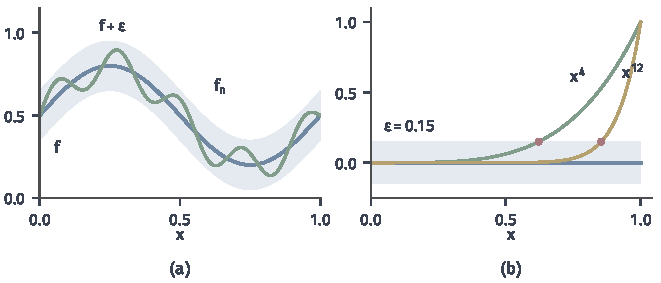
\includegraphics[width=112mm]{figures/04-spaces-measures-and-geometry/03-function-spaces/matplotlib/nspace-uniform-tube/figure.pdf}
  \caption{一致范数的几何意义，浅蓝色为半宽$\varepsilon=0.15$的带子。(a)$f(x)=0.5+0.3\sin(2\pi x)$（蓝）周围的带子，$f_n=f+0.1\sin(9\pi x)$（绿）整条曲线都在带内，所以$\lVert f_n-f\rVert_\infty=0.1$。(b)零函数周围的带子；$x^4$与$x^{12}$分别在红点$x=0.15^{1/4}$和$x=0.15^{1/12}$处越出带子。}
  \label{fig:nspace-uniform-tube}
\end{BookInlineFigure}

$x^n$在这个范数下连柯西列都不是。令$t=x^n$，当$x$跑遍$[0,1]$时$t$也跑遍$[0,1]$，所以
\[
 \lVert x^n-x^{2n}\rVert_\infty=\max_{t\in[0,1]}(t-t^2)=\frac14,
\]
这个值不随$n$减小。

\paragraph{完备性}
第~\ref{chap:metric-space-maps}章已经为一致收敛建立了两个结论：目标空间完备时，一致柯西的映射列一致收敛到某个映射；连续映射列的一致极限仍连续。$\mathbb K$是完备的，把两者合起来，就得到连续函数空间的完备性。

\begin{theorem}[紧集上连续函数空间的完备性]
\label{thm:nspace-ck-complete}
设$K$是非空紧度量空间。则$(C(K),\lVert\cdot\rVert_\infty)$是Banach空间。
\end{theorem}

\begin{proof}
设$(f_n)$是$C(K)$中的柯西列。对每个$\varepsilon>0$，存在$N$，使$m,n\geq N$时
\[
 \max_{x\in K}\lvert f_n(x)-f_m(x)\rvert<\varepsilon,
\]
这正说明$(f_n)$作为映射列是一致柯西的。

$\mathbb K$完备，所以$f_n$一致收敛到某个函数$f:K\to\mathbb K$。各$f_n$连续，一致极限$f$也连续，于是$f\in C(K)$。一致收敛就是$\lVert f_n-f\rVert_\infty\to0$，所以柯西列在$C(K)$中收敛。
\end{proof}

证明中三件事各有出处：候选极限由$\mathbb K$的完备性逐点给出；共同的误差阈值把逐点收敛加强为一致收敛；一致收敛保证极限连续。$K$的紧性只用来保证最大值有限，使式~\eqref{eq:nspace-uniform-norm}是范数。

\paragraph{非紧定义域}
在非紧的度量空间$X$上，连续函数可能无界，例如$\mathbb R$上的$f(x)=x$，一致“范数”不再是实数。这时只保留有界的连续函数，并把最大值换成上确界：
\begin{equation}
 C_b(X)=\Bigl\{f:X\to\mathbb K\ \text{连续}:\ \sup_{x\in X}\lvert f(x)\rvert<\infty\Bigr\},
 \label{eq:nspace-cb}
\end{equation}
范数为
\[
 \lVert f\rVert_\infty=\sup_{x\in X}\lvert f(x)\rvert.
\]
有界函数之和与数乘仍有界，所以$C_b(X)$是线性空间。

定理~\ref{thm:nspace-ck-complete}的证明中，候选极限的存在和连续都没有用到紧性。非紧时只需补充一步：一致极限仍然有界。取$N$使$n\geq N$时$\sup_x\lvert f_n(x)-f(x)\rvert\leq1$，则对每个$x$，
\[
 \lvert f(x)\rvert\leq\lvert f_N(x)\rvert+1\leq\lVert f_N\rVert_\infty+1,
\]
右边与$x$无关。于是$f\in C_b(X)$，所以$(C_b(X),\lVert\cdot\rVert_\infty)$对任意度量空间$X$都是Banach空间。

非紧定义域上会出现紧区间上没有的现象。在$C_b(\mathbb R)$中取移动的三角形
\[
 f_n(x)=\max\bigl(0,\ 1-\lvert x-n\rvert\bigr).
\]
每个固定的$x$在$n>\lvert x\rvert+1$以后都有$f_n(x)=0$，所以$f_n$逐点趋于零；但峰高始终为$1$，$\lVert f_n\rVert_\infty=1$，序列不依范数收敛。质量没有消失，只是移向无穷远，这与向量的单位列$e_n$的情形相同。

\paragraph{积分范数下的不完备}
回到$C[0,1]$，改用积分范数$\lVert f\rVert_1=\int_0^1\lvert f(x)\rvert\,dx$，其中积分对Lebesgue测度取，连续函数的Lebesgue积分与黎曼积分相同。集合没有变，只换了衡量误差的方式，完备性却会失去。

对$n\geq2$，令
\[
 g_n(x)=\begin{cases}0,&0\leq x\leq\frac12,\\ n\bigl(x-\frac12\bigr),&\frac12<x<\frac12+\frac1n,\\ 1,&\frac12+\frac1n\leq x\leq1.\end{cases}
\]
每个$g_n$连续，越来越陡地从$0$升到$1$，像是在逼近$\tfrac12$处跳跃的阶跃函数$\mathbf 1_{(1/2,1]}$，如图~\ref{fig:nspace-step-ramp}(a)所示。

\begin{BookInlineFigure}
  \centering
  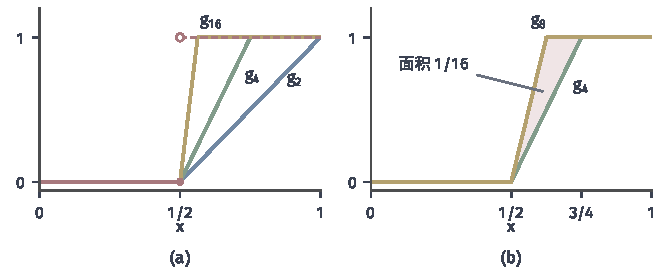
\includegraphics[width=112mm]{figures/04-spaces-measures-and-geometry/03-function-spaces/matplotlib/nspace-step-ramp/figure.pdf}
  \caption{积分范数下的柯西列。(a)折线$g_2,g_4,g_{16}$（蓝、绿、黄）越来越陡，红线是它们的积分极限$\mathbf 1_{(1/2,1]}$，空心圈表示跳跃。(b)$g_4$与$g_8$之间的浅红区域面积为$\lVert g_4-g_8\rVert_1=\tfrac1{16}$。}
  \label{fig:nspace-step-ramp}
\end{BookInlineFigure}

先算这列函数彼此的距离。设$m>n\geq2$，则$g_m\geq g_n$处处成立，所以
\[
 \lVert g_n-g_m\rVert_1=\int_0^1g_m\,dx-\int_0^1g_n\,dx.
\]
$g_n$下方的面积由一个底$\tfrac1n$、高$1$的三角形和宽$\tfrac12-\tfrac1n$的矩形组成，于是
\[
 \int_0^1g_n\,dx=\frac12-\frac1{2n}.
\]
代回前式，得到
\begin{equation}
 \lVert g_n-g_m\rVert_1=\frac1{2n}-\frac1{2m}.
 \label{eq:nspace-ramp-distance}
\end{equation}
例如$n=4$、$m=8$时距离是$\tfrac18-\tfrac1{16}=\tfrac1{16}$，就是图~\ref{fig:nspace-step-ramp}(b)中的面积。式~\eqref{eq:nspace-ramp-distance}小于$\tfrac1{2n}$，随$n$增大趋于零，所以$(g_n)$是柯西列。

下面证明它在$C[0,1]$中没有极限。假设存在$g\in C[0,1]$使$\lVert g_n-g\rVert_1\to0$。每个$g_n$在$[0,\tfrac12]$上为零，所以
\[
 \int_0^{1/2}\lvert g(x)\rvert\,dx\leq\int_0^1\lvert g_n(x)-g(x)\rvert\,dx\to0.
\]
左边不依赖$n$，只能为零；$\lvert g\rvert$连续且非负，故$g=0$在$[0,\tfrac12]$上处处成立。

再任取$\delta\in(0,\tfrac12)$。当$n>1/\delta$时，$g_n$在$[\tfrac12+\delta,1]$上恒为$1$，同样的论证给出
\[
 \int_{1/2+\delta}^1\lvert1-g(x)\rvert\,dx=0,
\]
所以$g=1$在$[\tfrac12+\delta,1]$上成立。$\delta$任意，所以$g$在$(\tfrac12,1]$上恒为$1$。于是$g(\tfrac12)=0$，而右侧极限为$1$，$g$在$\tfrac12$处不连续，矛盾。

所以$(C[0,1],\lVert\cdot\rVert_1)$不是Banach空间。同一列函数在一致范数下连柯西列都不是：取$x=\tfrac12+\tfrac1{2n}$，
\[
 \lvert g_{2n}(x)-g_n(x)\rvert=1-\frac12=\frac12.
\]

积分误差所指向的“极限”是阶跃函数，它不在连续函数之中，而且它在$\tfrac12$处取什么值并不影响积分。要让这样的极限有处可去，下一节把成员扩大为可测函数，并把几乎处处相等的函数看作同一个元素。

\section{\texorpdfstring{$L^p$}{Lp}空间}
\label{sec:nspace-lp-spaces}

上一节的折线列在积分误差下彼此越来越近，极限却是一个阶跃函数，不在连续函数之中。本节允许一般的可测函数，按$p$次幂累计偏差，并把在零测集上改动的函数看作同一个元素。这样得到的$L^p$空间满足范数公理，而且完备。

本节固定测度空间$(X,\mathcal A,\mu)$。可测函数、积分、单调收敛定理与Fatou引理见第~\ref{chap:measure}章和第~\ref{chap:integration}章。函数取值于$\mathbb K$，所有估计都只用到绝对值，实、复两种情形的论证相同。

\paragraph{几乎处处相等的函数}
在$[0,1]$上取Lebesgue测度，令$f\equiv0$，而$g$只在$x=\tfrac12$处取$1$、其余处取$0$。单点集的测度为零，所以$\int_0^1\lvert f-g\rvert\,dx=0$。用积分衡量误差时，这两个函数无法区分；若坚持把它们当作不同的元素，积分就只是半范数，正定性失效。

解决办法是把它们看作同一个元素。对两个可测函数，规定
\begin{equation}
 f\sim_\mu g\quad\Longleftrightarrow\quad \mu(\{x:f(x)\neq g(x)\})=0,
 \label{eq:nspace-ae-equivalence}
\end{equation}
即$f=g$在$\mu$下\term{几乎处处}（almost everywhere）成立。这是等价关系：自反与对称直接成立；若$f\sim_\mu g$且$g\sim_\mu h$，则
\[
 \{f\neq h\}\subseteq\{f\neq g\}\cup\{g\neq h\},
\]
两个零测集之并仍是零测集。与$f$几乎处处相等的可测函数全体记为$[f]$，称为$f$的\term{等价类}（equivalence class），$f$是它的一个代表。

等价类之间的运算借助代表定义：$[f]+[g]=[f+g]$，$c[f]=[cf]$。结果不依赖代表的选择：若$f'\sim_\mu f$、$g'\sim_\mu g$，则
\[
 \{f'+g'\neq f+g\}\subseteq\{f'\neq f\}\cup\{g'\neq g\}
\]
是零测集。所以可测函数的等价类组成线性空间，零元素是几乎处处为零的函数这一整类。

把函数看作向量时，这一步相当于放弃了“读取单个分量”。在Lebesgue测度下每个单点都是零测集，同一类中的代表可以在任意给定点取任意值，“$[f]$在$x_0$处的值”没有意义。若$\mu(\{x_0\})>0$，同一类的代表在$x_0$处必须取同一个值。点值读取何时有意义，是第~\ref{chap:linear-functionals}章和第~\ref{chap:rkhs}章的问题。

\paragraph{\texorpdfstring{$L^p$}{Lp}范数}
有了等价类，就可以用$p$次幂的积分衡量函数的大小。这相当于把向量的$p$范数$(\sum_i\lvert v_i\rvert^p)^{1/p}$中的求和换成积分。

\begin{definition}[$L^p$空间]
\label{def:nspace-lp}
设$1\leq p<\infty$。若可测函数$f$满足$\int_X\lvert f\rvert^p\,d\mu<\infty$，称$f$是$p$次可积的。$p$次可积函数的几乎处处等价类全体记为$L^p(\mu)$，并令
\begin{equation}
 \lVert f\rVert_p=\Bigl(\int_X\lvert f\rvert^p\,d\mu\Bigr)^{1/p}.
 \label{eq:nspace-lp-norm}
\end{equation}
当$X$是欧氏空间的可测子集$\Omega$、$\mu$为Lebesgue测度时，记为$L^p(\Omega)$。
\end{definition}

这里用代表$f$代写等价类$[f]$。定义需要核验三件事。其一，数值不依赖代表：若$f\sim_\mu g$，则$\lvert f\rvert^p$与$\lvert g\rvert^p$几乎处处相等，零测集上的改动不影响积分。其二，正定性：$\int\lvert f\rvert^p\,d\mu=0$当且仅当$\lvert f\rvert^p=0$几乎处处，即$[f]$是零元素，这正是引入等价类要换取的结果。齐次性直接由积分的线性得到。

其三，$L^p(\mu)$对加法封闭。$p\geq1$时函数$t\mapsto t^p$在$[0,\infty)$上凸，所以对$a,b\geq0$有
\[
 \Bigl(\frac{a+b}2\Bigr)^p\leq\frac{a^p+b^p}2,
\]
也就是$(a+b)^p\leq2^{p-1}(a^p+b^p)$。取$a=\lvert f(x)\rvert$、$b=\lvert g(x)\rvert$，由$\lvert f+g\rvert\leq a+b$积分得
\[
 \int_X\lvert f+g\rvert^p\,d\mu\leq2^{p-1}\Bigl(\int_X\lvert f\rvert^p\,d\mu+\int_X\lvert g\rvert^p\,d\mu\Bigr)<\infty.
\]
数乘只把积分乘以常数$\lvert c\rvert^p$，封闭性同样成立，所以$L^p(\mu)$是线性空间。剩下的三角不等式不能由这个粗略估计得到，要用下面的Hölder不等式。

\paragraph{不同的\texorpdfstring{$p$}{p}}
$p$越大，局部的大偏差在总量中所占的比重越大。比较$[0,1]$上的两个误差：$h_1\equiv1$处处偏差为$1$，$h_2=4\cdot\mathbf 1_{[0,1/4]}$只在四分之一的区间上偏差为$4$。按绝对值累计，两者一样大：
\[
 \lVert h_1\rVert_1=1,\qquad \lVert h_2\rVert_1=4\times\frac14=1.
\]
按平方累计，分散的误差仍是$1$，集中的误差翻了一倍：
\[
 \lVert h_1\rVert_2=1,\qquad \lVert h_2\rVert_2=\Bigl(16\times\frac14\Bigr)^{1/2}=2.
\]

一般地，同样的计算给出
\[
 \lVert h_2\rVert_p=\Bigl(4^p\cdot\frac14\Bigr)^{1/p}=4^{1-1/p},
\]
它随$p$增大而增大，趋于最大偏差$4$，见图~\ref{fig:nspace-lp-weight}。选择$p$就是选择怎样为大偏差计价。

\begin{BookInlineFigure}
  \centering
  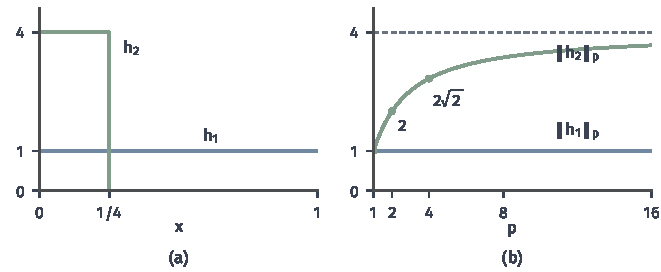
\includegraphics[width=112mm]{figures/04-spaces-measures-and-geometry/03-function-spaces/matplotlib/nspace-lp-weight/figure.pdf}
  \caption{$L^p$范数对大偏差的计价。(a)$[0,1]$上的两个误差：蓝色的$h_1\equiv1$与绿色的$h_2=4\cdot\mathbf 1_{[0,1/4]}$，二者$L^1$范数都是$1$。(b)$\lVert h_1\rVert_p\equiv1$，而$\lVert h_2\rVert_p=4^{1-1/p}$，在$p=1,2,4$处依次为$1,2,2\sqrt2$，虚线是$p\to\infty$时的极限$4$。}
  \label{fig:nspace-lp-weight}
\end{BookInlineFigure}

可积性也随$p$改变。在$(0,1]$上，$x^{-1/2}$属于$L^1$，因为
\[
 \int_0^1x^{-1/2}\,dx=2.
\]
它不属于$L^2$，因为$\int_0^1x^{-1}\,dx=\infty$。$x^{-1/4}$属于$L^2$，平方积分为$2$，但它在$0$附近无界。

\paragraph{数列空间}
取$X=\mathbb N_+$与\term{计数测度}（counting measure），即每个点的测度为$1$。可测函数就是数列$x=(x_k)$，积分就是求和，只有空集零测，等价类就是数列本身。$L^p$成为
\begin{equation}
 \ell^p=\Bigl\{x:\ \sum_{k\geq1}\lvert x_k\rvert^p<\infty\Bigr\},\quad \lVert x\rVert_p=\Bigl(\sum_{k\geq1}\lvert x_k\rvert^p\Bigr)^{1/p}.
 \label{eq:nspace-ellp}
\end{equation}
这是函数作为无限维向量最直接的情形：有限维向量可以看作后面全为零的数列，$\lVert x\rVert_p$就是卷二的坐标$p$范数的延伸。数列$x_k=1/k$属于$\ell^2$，因为$\sum_k1/k^2$收敛；它不属于$\ell^1$，因为调和级数发散。

\paragraph{Hölder与Minkowski不等式}
三角不等式的证明，关键在于控制乘积的积分。设$1<p<\infty$，取$q$满足$\tfrac1p+\tfrac1q=1$，即$q=p/(p-1)$，称$p,q$为\term{共轭指数}（conjugate exponents）。例如$p=2$时$q=2$，$p=3$时$q=\tfrac32$。

在有限维中，向量分量乘积之和有基本估计
\[
 \Bigl\lvert\sum_iu_iv_i\Bigr\rvert\leq\lVert u\rVert_p\lVert v\rVert_q,
\]
$p=q=2$时就是Cauchy--Schwarz不等式。下面把它搬到积分上，先从两个数的乘积开始。

\begin{lemma}[Young不等式]
\label{lem:nspace-young}
设$1<p<\infty$，$q$为其共轭指数。对任意$a,b\geq0$，
\begin{equation}
 ab\leq\frac{a^p}{p}+\frac{b^q}{q},
 \label{eq:nspace-young}
\end{equation}
等号当且仅当$a^p=b^q$。
\end{lemma}

\begin{proof}
固定$b\geq0$，考察$s\geq0$上的函数
\[
 F(s)=\frac{s^p}{p}-bs.
\]
求导得$F'(s)=s^{p-1}-b$，它在$s_*=b^{1/(p-1)}$处为零，在$s<s_*$时为负、$s>s_*$时为正，所以$F$在$s_*$处取唯一的最小值。

由$p/(p-1)=q$得$s_*^p=b^q$，又$bs_*=b^{1+1/(p-1)}=b^q$。代入$F$，于是
\[
 F(s_*)=\frac{b^q}{p}-b^q=-\frac{b^q}{q}.
\]
所以$F(a)\geq-b^q/q$，移项即得不等式；等号当且仅当$a=s_*$，即$a^p=b^q$。
\end{proof}

这个不等式有一幅面积图像。共轭条件等价于$(p-1)(q-1)=1$，所以曲线$s=t^{p-1}$也可以写成$t=s^{q-1}$。如图~\ref{fig:nspace-young-area}所示，曲线下方从$0$到$a$的面积是$a^p/p$，曲线左方从$0$到$b$的面积是$b^q/q$，两块区域合起来盖住矩形$[0,a]\times[0,b]$，所以面积之和不小于$ab$。

\begin{BookInlineFigure}
  \centering
  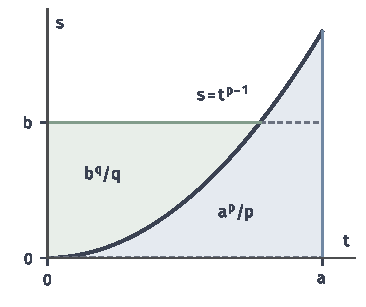
\includegraphics[width=62mm]{figures/04-spaces-measures-and-geometry/03-function-spaces/matplotlib/nspace-young-area/figure.pdf}
  \caption{Young不等式的面积解释，取$p=3$、$q=\tfrac32$、$a=1$、$b=0.6$。曲线为$s=t^2$，蓝色区域面积$a^p/p=\tfrac13$，绿色区域面积$b^q/q\approx0.310$，二者盖住虚线所示面积为$ab=0.6$的矩形。只有曲线恰好穿过矩形右上角，即$b=a^{p-1}$时，两块区域才恰好拼成矩形。}
  \label{fig:nspace-young-area}
\end{BookInlineFigure}

用图中的数字验算：$ab=0.6$，而$\tfrac13+0.310=0.643$，不等式成立且是严格的。若把$b$取成$a^{p-1}=1$，则$ab=1=\tfrac13+\tfrac23$，等号成立。

\begin{theorem}[Hölder不等式]
\label{thm:nspace-holder}
设$1<p<\infty$，$q$为其共轭指数，$f,g$是$X$上的可测函数。则
\begin{equation}
 \int_X\lvert fg\rvert\,d\mu\leq\lVert f\rVert_p\,\lVert g\rVert_q ,
 \label{eq:nspace-holder}
\end{equation}
其中右边允许取$+\infty$。特别地，$f\in L^p(\mu)$、$g\in L^q(\mu)$时$fg\in L^1(\mu)$。
\end{theorem}

\begin{proof}
若右边为$+\infty$，无需证明。若$\lVert f\rVert_p=0$，则$f=0$几乎处处，$fg=0$几乎处处，左边为零；$\lVert g\rVert_q=0$同理。下设$0<\lVert f\rVert_p,\lVert g\rVert_q<\infty$。

在Young不等式中逐点取$a=\lvert f(x)\rvert/\lVert f\rVert_p$、$b=\lvert g(x)\rvert/\lVert g\rVert_q$，得到
\[
 \frac{\lvert f(x)g(x)\rvert}{\lVert f\rVert_p\lVert g\rVert_q}\leq\frac{\lvert f(x)\rvert^p}{p\lVert f\rVert_p^p}+\frac{\lvert g(x)\rvert^q}{q\lVert g\rVert_q^q}.
\]
两边积分，右边等于$\tfrac1p+\tfrac1q=1$，再乘以$\lVert f\rVert_p\lVert g\rVert_q$即得结论。
\end{proof}

归一化的作用是把两个任意大小的函数缩放到“单位大小”，使右边两项积分后恰好凑成$1$。在$[0,1]$上取$f=x$、$g=x^2$、$p=3$、$q=\tfrac32$，此时$\lvert f\rvert^3=x^3=\lvert g\rvert^{3/2}$，两边相等：
\[
 \int_0^1x^3\,dx=\frac14,\qquad \Bigl(\frac14\Bigr)^{1/3}\Bigl(\frac14\Bigr)^{2/3}=\frac14,
\]
这与Young不等式的等号条件$a^p=b^q$相符。若取$f=1$、$g=x$、$p=q=2$，左边为$\tfrac12$，右边为$(\tfrac13)^{1/2}\approx0.577$，不等式是严格的。

\begin{theorem}[Minkowski不等式]
\label{thm:nspace-minkowski}
设$1\leq p<\infty$，$f,g\in L^p(\mu)$。则
\begin{equation}
 \lVert f+g\rVert_p\leq\lVert f\rVert_p+\lVert g\rVert_p.
 \label{eq:nspace-minkowski}
\end{equation}
因此$(L^p(\mu),\lVert\cdot\rVert_p)$是赋范空间。
\end{theorem}

\begin{proof}
$p=1$时，对逐点不等式$\lvert f+g\rvert\leq\lvert f\rvert+\lvert g\rvert$积分即可。

设$1<p<\infty$，记$I=\int\lvert f+g\rvert^p\,d\mu$。由封闭性的估计，$I<\infty$；若$I=0$，结论平凡，下设$I>0$。先把$p$次幂拆成两项：
\[
 \lvert f+g\rvert^p\leq\lvert f+g\rvert^{p-1}\lvert f\rvert+\lvert f+g\rvert^{p-1}\lvert g\rvert.
\]

由$(p-1)q=p$，$\lvert f+g\rvert^{p-1}$的$q$次积分等于$I$，所以它的$L^q$范数是$I^{1/q}$。对右边两项分别用Hölder不等式，
\[
 \int\lvert f+g\rvert^{p-1}\lvert f\rvert\,d\mu\leq I^{1/q}\lVert f\rVert_p,
\]
\[
 \int\lvert f+g\rvert^{p-1}\lvert g\rvert\,d\mu\leq I^{1/q}\lVert g\rVert_p.
\]

相加，得到
\[
 I\leq I^{1/q}\bigl(\lVert f\rVert_p+\lVert g\rVert_p\bigr).
\]
两边除以$I^{1/q}$（它有限且为正），由$1-\tfrac1q=\tfrac1p$得$I^{1/p}\leq\lVert f\rVert_p+\lVert g\rVert_p$，这就是结论。
\end{proof}

证明中的除法要求$I$有限且为正：有限性来自封闭性估计，正性单独处理。若只知道$I\leq I^{1/q}(\cdots)$而不知$I<\infty$，两边可能都是$\infty$，推不出结论。

\paragraph{完备性}
现在回答本节开头的问题：积分误差下的柯西列是否一定有极限。困难在于$L^p$范数只控制积分，不控制每一点：柯西列在单个点处可能根本不收敛。第~\ref{sec:nspace-convergence-of-sequences}节的打字机序列就是这样。

下面的证明先抽出一个相邻误差可求和的子列，借它得到几乎处处收敛的候选极限，再用Fatou引理把逐点信息转回积分。

\begin{theorem}[$L^p$的完备性]
\label{thm:nspace-lp-complete}
对任意测度空间与$1\leq p<\infty$，$L^p(\mu)$是Banach空间。
\end{theorem}

\begin{proof}
设$(f_n)$是$L^p(\mu)$中的柯西列，取定各项的可测代表。

第一步，抽取快速子列。由柯西条件，可以递归地取$n_1<n_2<\cdots$，使$m,n\geq n_k$时$\lVert f_n-f_m\rVert_p<2^{-k}$。于是
\[
 \lVert f_{n_{k+1}}-f_{n_k}\rVert_p<2^{-k},\qquad \sum_{k\geq1}\lVert f_{n_{k+1}}-f_{n_k}\rVert_p<\infty.
\]

第二步，构造控制函数。令
\[
 S_m=\lvert f_{n_1}\rvert+\sum_{k=1}^m\lvert f_{n_{k+1}}-f_{n_k}\rvert,\qquad S=\lim_{m\to\infty}S_m\in[0,\infty].
\]
由Minkowski不等式，$S_m$的范数有一个与$m$无关的上界：
\[
 \lVert S_m\rVert_p\leq\lVert f_{n_1}\rVert_p+\sum_{k\geq1}\lVert f_{n_{k+1}}-f_{n_k}\rVert_p=:C<\infty.
\]
$S_m^p$逐点单调上升到$S^p$，由单调收敛定理，
\[
 \int_XS^p\,d\mu=\lim_{m\to\infty}\int_XS_m^p\,d\mu\leq C^p.
\]
所以$S<\infty$几乎处处。

第三步，定义候选极限。在$\{S<\infty\}$上，级数$f_{n_1}+\sum_k(f_{n_{k+1}}-f_{n_k})$绝对收敛，它的第$k$个部分和就是$f_{n_{k+1}}$；令$f$为其和，在零测集$\{S=\infty\}$上令$f=0$。$f$是可测函数列的几乎处处极限，因而可测，并且$\lvert f\rvert\leq S$，所以$f\in L^p(\mu)$。

第四步，子列依范数收敛。固定$j$。在$\{S<\infty\}$上，
\[
 \lvert f-f_{n_j}\rvert^p=\lim_{m\to\infty}\lvert f_{n_m}-f_{n_j}\rvert^p.
\]
由Fatou引理，
\[
 \int_X\lvert f-f_{n_j}\rvert^p\,d\mu\leq\liminf_{m\to\infty}\int_X\lvert f_{n_m}-f_{n_j}\rvert^p\,d\mu.
\]
把差写成相邻差之和，
\[
 f_{n_m}-f_{n_j}=\sum_{k=j}^{m-1}\bigl(f_{n_{k+1}}-f_{n_k}\bigr),
\]
再用Minkowski不等式，得到
\[
 \lVert f-f_{n_j}\rVert_p\leq\sum_{k\geq j}\lVert f_{n_{k+1}}-f_{n_k}\rVert_p.
\]
右边是收敛级数的尾和，趋于零，所以$\lVert f_{n_j}-f\rVert_p\to0$。

第五步，回到整列。给定$\varepsilon>0$，取$N$使$m,n\geq N$时$\lVert f_n-f_m\rVert_p<\varepsilon$，再取$j$使$n_j\geq N$且$\lVert f_{n_j}-f\rVert_p<\varepsilon$。则$n\geq N$时
\[
 \lVert f_n-f\rVert_p\leq\lVert f_n-f_{n_j}\rVert_p+\lVert f_{n_j}-f\rVert_p<2\varepsilon.
\]
\end{proof}

五步各有职责。第一步的快速子列使控制函数$S$的范数有限；第二步由此得到$S<\infty$几乎处处，候选极限才有定义；第四步的Fatou引理把几乎处处的收敛转化为积分误差的估计；最后一步说明：柯西列只要有一个子列收敛，整列就收敛到同一极限。

图~\ref{fig:nspace-fast-subsequence}用一列具体的函数显示了第二步的控制。部分和不断加上越来越小的修正，$S_m$把所有修正的绝对值累计起来，单调上升但有界；$f_{n_k}$始终夹在$-S$和$S$之间，所以每个$S<\infty$的点处级数都绝对收敛。

\begin{BookInlineFigure}
  \centering
  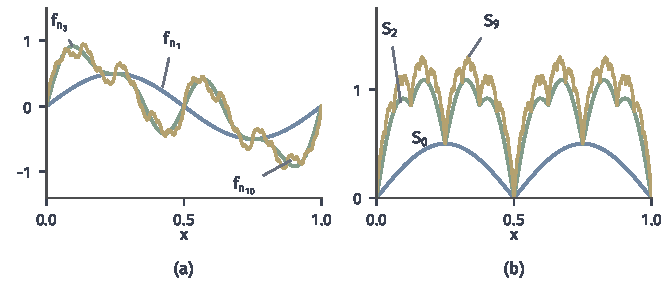
\includegraphics[width=112mm]{figures/04-spaces-measures-and-geometry/03-function-spaces/matplotlib/nspace-fast-subsequence/figure.pdf}
  \caption{完备性证明中的快速子列与控制函数。这里$f_{n_1}(x)=\tfrac12\sin(2\pi x)$，相邻差$f_{n_{k+1}}-f_{n_k}=2^{-k}\sin(2^{k+1}\pi x)$。(a)$f_{n_1},f_{n_3},f_{n_{10}}$，修正项越来越小。(b)控制函数$S_0,S_2,S_9$，随$m$单调上升且有界，每一项$\lvert f_{n_k}\rvert$都不超过它们的极限$S$。}
  \label{fig:nspace-fast-subsequence}
\end{BookInlineFigure}

\begin{theorem}[$L^p$收敛列的几乎处处收敛子列]
\label{thm:nspace-lp-ae-subsequence}
设$1\leq p<\infty$，在$L^p(\mu)$中$f_n\to f$。则存在子列$(f_{n_k})$，使$f_{n_k}\to f$几乎处处成立。
\end{theorem}

\begin{proof}
收敛列是柯西列。定理~\ref{thm:nspace-lp-complete}证明的前四步给出子列与函数$\tilde f$，使$f_{n_k}\to\tilde f$几乎处处且在$L^p$中成立。$L^p$中的极限唯一，所以$\tilde f=f$几乎处处，于是$f_{n_k}\to f$几乎处处。
\end{proof}

回到上一节的折线列$(g_n)$，把证明的步骤走一遍。在$L^1[0,1]$中，阶跃函数的等价类$\mathbf 1_{(1/2,1]}$是合法的元素。由式~\eqref{eq:nspace-ramp-distance}，取$n_k=2^k$时相邻误差为
\[
 \lVert g_{2^{k+1}}-g_{2^k}\rVert_1=\frac1{2^{k+1}}-\frac1{2^{k+2}}=2^{-k-2},
\]
对$k\geq1$求和得$\tfrac14$。

$g_n$关于$n$单调不减，所以控制函数中的绝对值可以去掉，并逐项相消：
\[
 S_m=g_2+\sum_{k=1}^m\bigl(g_{2^{k+1}}-g_{2^k}\bigr)=g_{2^{m+1}}.
\]
令$m\to\infty$，得到$S=\mathbf 1_{(1/2,1]}$，这正是候选极限。它的范数$\lVert S\rVert_1=\tfrac12$，恰好等于证明中的上界$C=\lVert g_2\rVert_1+\tfrac14=\tfrac14+\tfrac14$。

最后计算依范数的误差。折线与阶跃函数只在一个底为$\tfrac1n$、高为$1$的三角形上不同，所以
\[
 \lVert g_n-\mathbf 1_{(1/2,1]}\rVert_1=\frac1{2n}\to0.
\]
在$L^1$中折线列有了极限。阶跃函数在$\tfrac12$处取什么值无关紧要，这正是取等价类的用意。在计数测度下，定理~\ref{thm:nspace-lp-complete}说明每个$\ell^p$（$1\leq p<\infty$）都是Banach空间。

\section{\texorpdfstring{$L^\infty$}{L-infinity}空间}
\label{sec:nspace-linfty-space}

图~\ref{fig:nspace-lp-weight}显示，$p$越大，$L^p$范数越看重大偏差，$p\to\infty$时只剩下最大偏差。向量的情形正是这样：$\lVert v\rVert_p\to\max_i\lvert v_i\rvert$。但等价类中的代表可以在零测集上任意改值，普通的上确界会被单个点左右，对等价类没有确定的意义。本节建立只看“几乎处处”的上界，得到$L^\infty$空间。本节仍固定测度空间$(X,\mathcal A,\mu)$。

\paragraph{本质上确界}
普通上确界要求$\lvert f(x)\rvert\leq M$在每一点都成立；对等价类而言，合理的要求是在某个零测集之外成立。

\begin{definition}[本质上确界与$L^\infty$]
\label{def:nspace-linfty}
对可测函数$f$，定义
\begin{equation}
 \lVert f\rVert_\infty=\inf\{M\geq0:\ \mu(\{x:\lvert f(x)\rvert>M\})=0\},
 \label{eq:nspace-esssup}
\end{equation}
称为$\lvert f\rvert$的\term{本质上确界}（essential supremum），约定空集的下确界为$+\infty$。本质上确界有限的可测函数称为\term{本质有界}（essentially bounded）的，其几乎处处等价类全体记为$L^\infty(\mu)$。
\end{definition}

先看下确界能否取到。设$M_0=\lVert f\rVert_\infty<\infty$。对每个正整数$k$，$M_0+1/k$大于下确界，所以$\{\lvert f\rvert>M_0+1/k\}$是零测集。它们的并
\[
 \{\lvert f\rvert>M_0\}=\bigcup_{k\geq1}\Bigl\{\lvert f\rvert>M_0+\frac1k\Bigr\}
\]
是可数个零测集之并，仍为零测集。所以下确界可以达到：
\begin{equation}
 \lvert f\rvert\leq\lVert f\rVert_\infty\quad\text{几乎处处}.
 \label{eq:nspace-esssup-attained}
\end{equation}
由此也看出数值不依赖代表：若$g\sim_\mu f$，则$\{\lvert g\rvert>M\}\subseteq\{\lvert f\rvert>M\}\cup\{f\neq g\}$，反之亦然，两者的本质上确界相同。

\paragraph{与逐点上确界的比较}
本质上确界与普通上确界可以相差很远。在$[0,1]$上取Lebesgue测度，令$f(x)=x$，再把$f(\tfrac12)$改为$2$。普通上确界是$2$；而$\lvert f\rvert\leq1$只在单点$\{\tfrac12\}$处不成立，单点零测，所以本质上确界是$1$，如图~\ref{fig:nspace-essential-sup}所示。

\begin{BookInlineFigure}
  \centering
  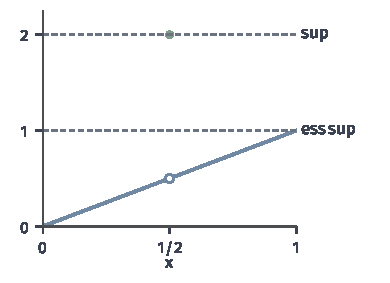
\includegraphics[width=66mm]{figures/04-spaces-measures-and-geometry/03-function-spaces/matplotlib/nspace-essential-sup/figure.pdf}
  \caption{本质上确界忽略零测集。$[0,1]$上取Lebesgue测度，$f(x)=x$，只把$f(\tfrac12)$改为$2$（绿点为改动后的值，空心圈为原值）。普通上确界被这一个点抬到$2$，单点的测度为零，本质上确界仍为$1$。}
  \label{fig:nspace-essential-sup}
\end{BookInlineFigure}

更极端地，有理点的指示函数$\mathbf 1_{\mathbb Q\cap[0,1]}$的普通上确界是$1$，本质上确界是$0$，因为有理点只有可数个，组成零测集。

两者在一个常见情形下一致。若$f$在区间$[a,b]$上连续，对任意$M<\sup\lvert f\rvert$，集合$\{\lvert f\rvert>M\}$是非空的相对开集，含有一个正长度的区间，测度为正，所以本质上确界不小于普通上确界，二者相等。另一方面，$\lVert f\rVert_\infty\leq M$只保证零测集之外$\lvert f\rvert\leq M$，并不保证类中任意一个代表在每一点都受这个界控制。

取$\mathbb N_+$上的计数测度，只有空集零测，本质上确界就是普通上确界，得到有界数列空间
\begin{equation}
 \ell^\infty=\Bigl\{x:\ \sup_{k}\lvert x_k\rvert<\infty\Bigr\},\qquad \lVert x\rVert_\infty=\sup_k\lvert x_k\rvert.
 \label{eq:nspace-ellinfty}
\end{equation}
常数列$(1,1,\ldots)$属于$\ell^\infty$，却不属于任何$\ell^p$（$p<\infty$）。第~\ref{chap:functions-as-vectors}章用$\ell^\infty$中两两距离为$1$的不可数个$0$--$1$数列，说明了它没有可数的级数表示。

\paragraph{范数公理}
$\lVert\cdot\rVert_\infty$在$L^\infty(\mu)$上是范数，论证的关键是把例外集合合并成一个零测集。

正定性：若$\lVert f\rVert_\infty=0$，由式~\eqref{eq:nspace-esssup-attained}，$\lvert f\rvert\leq0$几乎处处，即$[f]$是零元素。齐次性：$c\neq0$时，
\[
 \{\lvert cf\rvert>\lvert c\rvert M\}=\{\lvert f\rvert>M\},
\]
对$M$取下确界即得；$c=0$时两边都是零。

三角不等式：$\lvert f\rvert\leq\lVert f\rVert_\infty$在零测集$N_f$之外成立，$\lvert g\rvert\leq\lVert g\rVert_\infty$在零测集$N_g$之外成立。于是在$N_f\cup N_g$之外，
\[
 \lvert f+g\rvert\leq\lvert f\rvert+\lvert g\rvert\leq\lVert f\rVert_\infty+\lVert g\rVert_\infty.
\]
例外集仍是零测集，所以右边是$\lvert f+g\rvert$的一个本质上界，三角不等式成立。这同时说明$L^\infty(\mu)$对加法封闭。

\paragraph{\texorpdfstring{$L^1$}{L1}与\texorpdfstring{$L^\infty$}{L-infinity}的Hölder估计}
Hölder不等式要求$1<p<\infty$。在端点处，$p=1$的共轭指数应当是$q=\infty$，相应的估计是：若$f\in L^1(\mu)$、$g\in L^\infty(\mu)$，则
\begin{equation}
 \int_X\lvert fg\rvert\,d\mu\leq\lVert f\rVert_1\,\lVert g\rVert_\infty .
 \label{eq:nspace-holder-endpoint}
\end{equation}

证明只需一步。由式~\eqref{eq:nspace-esssup-attained}，几乎处处有
\[
 \lvert fg\rvert\leq\lvert f\rvert\,\lVert g\rVert_\infty,
\]
两边积分即可。约定$1/\infty=0$后，Hölder不等式对所有满足$\tfrac1p+\tfrac1q=1$的$1\leq p,q\leq\infty$都成立。

这个估计说明，固定$g\in L^\infty$，$f\mapsto\int fg\,d\mu$是$L^1$上的线性读取，其大小受$\lVert g\rVert_\infty\lVert f\rVert_1$控制。第~\ref{chap:linear-functionals}章将从这样的配对出发研究$L^p$上的线性泛函。

\paragraph{完备性}
$L^\infty$的完备性与$L^p$（$p<\infty$）的证明方式不同。这里没有积分可以累计，却可以把可数个例外集合并成一个零测集，在它的补集上回到一致收敛的论证。

\begin{theorem}[$L^\infty$的完备性]
\label{thm:nspace-linfty-complete}
对任意测度空间，$L^\infty(\mu)$是Banach空间。
\end{theorem}

\begin{proof}
设$(f_n)$是$L^\infty(\mu)$中的柯西列，取定各项的可测代表。对每一对$m,n$，由式~\eqref{eq:nspace-esssup-attained}，在某个零测集$E_{m,n}$之外有
\[
 \lvert f_n-f_m\rvert\leq\lVert f_n-f_m\rVert_\infty.
\]
令$E=\bigcup_{m,n}E_{m,n}$，它是可数个零测集之并，仍为零测集。

在$X\setminus E$上，所有这些不等式同时成立。给定$\varepsilon>0$，取$N$使$m,n\geq N$时$\lVert f_n-f_m\rVert_\infty<\varepsilon$，则
\[
 \sup_{x\notin E}\lvert f_n(x)-f_m(x)\rvert\leq\varepsilon,\qquad m,n\geq N,
\]
即$(f_n)$在$X\setminus E$上一致柯西。$\mathbb K$完备，所以$f_n$在$X\setminus E$上一致收敛到某个函数$f$；在$E$上令$f=0$。$f$是可测函数列在$X\setminus E$上的逐点极限，因而可测。

在上式中令$m\to\infty$，得到$n\geq N$时
\[
 \sup_{x\notin E}\lvert f_n(x)-f(x)\rvert\leq\varepsilon.
\]
$E$零测，所以$\lVert f_n-f\rVert_\infty\leq\varepsilon$，即$f_n\to f$依范数成立。最后，取$n_0\geq N$，由三角不等式，
\[
 \lVert f\rVert_\infty\leq\lVert f_{n_0}\rVert_\infty+\varepsilon<\infty,
\]
所以$f\in L^\infty(\mu)$。
\end{proof}

两种完备性证明可以对照着看。有限$p$的论证没有一致性可用，只能先抽子列得到几乎处处收敛，再用Fatou引理把逐点信息转为积分信息。$p=\infty$的论证则把可数个例外集合并成一个零测集，在补集上做一致收敛，与连续函数空间的论证相同，只是“处处”换成了“零测集之外”。

在计数测度下，这个定理说明$\ell^\infty$是Banach空间。

\section{函数列的收敛}
\label{sec:nspace-convergence-of-sequences}

有了具体的赋范函数空间，同一列函数就可以在几种意义下讨论收敛：每个输入处的值是否收敛，所有输入上的最大误差是否趋于零，积分误差是否趋于零，误差超过给定阈值的区域是否越来越小。把函数看作向量时，它们分别对应“逐分量”“最大分量”“加权和”和“超差分量的份额”。

有限维向量的这几种收敛等价，函数列的收敛方式之间却只有在附加条件下才能互相推出。第~\ref{chap:integration}章已经用逐点与几乎处处收敛建立了单调收敛和支配收敛定理，本节把这些收敛方式放在一起比较，并用一致可积性补上从依测度收敛到$L^1$收敛所需的条件。

本节固定测度空间$(X,\mathcal A,\mu)$与一列可测函数$f_n$及可测函数$f$，它们几乎处处取有限值。

\subsection{逐点、一致与\texorpdfstring{$L^p$}{Lp}收敛}
\label{sec:nspace-pointwise-uniform-lp}

逐点收敛与一致收敛是对函数本身的要求，第~\ref{chap:metric-space-maps}章已经定义：逐点收敛允许达到给定精度所需的序号依赖于$x$，一致收敛要求同一个序号对所有$x$有效。$L^p$收敛（$1\leq p<\infty$）则是$\lVert f_n-f\rVert_p\to0$，它只看误差$p$次幂的积分。

\paragraph{代表的选择}
这三种收敛对零测集的态度不同。逐点收敛和一致收敛是对选定的代表说的：把$f_n$在一个零测集上改值，可能破坏逐点收敛，也可能把一致收敛的序列变得不一致收敛。

所以在等价类上讨论时，应当改用两个说法。一是几乎处处收敛，即存在零测集$E$使$f_n(x)\to f(x)$对$x\notin E$成立；二是本质一致收敛，即$\lVert f_n-f\rVert_\infty\to0$。

$L^p$收敛和下一小节的依测度收敛只依赖等价类：改动零测集上的值不改变任何积分，也不改变任何集合的测度。

\paragraph{一致收敛推出\texorpdfstring{$L^p$}{Lp}收敛的条件}
一致收敛控制所有点上的误差，积分误差自然也受控制，但这需要总测度有限。若$\mu(X)<\infty$，由$\lvert f_n-f\rvert\leq\lVert f_n-f\rVert_\infty$几乎处处成立，取$p$次幂后积分，得到
\begin{equation}
 \lVert f_n-f\rVert_p\leq\mu(X)^{1/p}\,\lVert f_n-f\rVert_\infty ,
 \label{eq:nspace-uniform-to-lp}
\end{equation}
所以本质一致收敛推出每个$L^p$收敛。测度无限时这一推论失败。在$\mathbb R$上取Lebesgue测度与$h_n=\tfrac1n\mathbf 1_{[0,n]}$，则
\[
 \lVert h_n\rVert_\infty=\frac1n\to0,\qquad \lVert h_n\rVert_1=1.
\]
高度在降低，支撑却在扩大，总面积不变。

不同指数之间也有类似的比较，同样依赖有限测度。设$\mu(X)<\infty$，$1\leq p<r<\infty$。对$\lvert h\rvert^p\cdot1$用Hölder不等式，指数取$r/p$及其共轭指数$r/(r-p)$，得到
\[
 \int_X\lvert h\rvert^p\,d\mu\leq\Bigl(\int_X\lvert h\rvert^r\,d\mu\Bigr)^{p/r}\mu(X)^{1-p/r}.
\]
两边开$p$次方，整理成
\begin{equation}
 \lVert h\rVert_p\leq\mu(X)^{1/p-1/r}\lVert h\rVert_r.
 \label{eq:nspace-lp-inclusion}
\end{equation}
取$h=f_n-f$，$L^r$收敛推出$L^p$收敛。把式~\eqref{eq:nspace-lp-inclusion}看作包含映射$L^r\to L^p$的有界性，是第~\ref{chap:linear-operators}章的内容。

\paragraph{三个对照序列}
图~\ref{fig:nspace-convergence-modes}与表~\ref{tab:nspace-convergence-modes}对照了$[0,1]$上Lebesgue测度下的三个序列，它们标出了各收敛方式之间不能互推的边界。

\begin{BookInlineFigure}
  \centering
  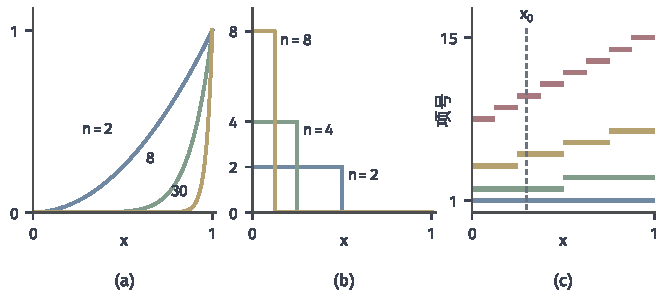
\includegraphics[width=112mm]{figures/04-spaces-measures-and-geometry/03-function-spaces/matplotlib/nspace-convergence-modes/figure.pdf}
  \caption{三种收敛方式的反例。(a)$x^n$，$n=2,8,30$：除$x=1$外逐点趋于$0$，$L^p$范数趋于零，最大误差恒为$1$。(b)窄尖峰$n\mathbf 1_{(0,1/n)}$，$n=2,4,8$：每一点最终为零，积分恒为$1$。(c)打字机序列的前$15$项，第$k$层（$k=0,1,2,3$，蓝、绿、黄、红）把$[0,1)$等分为$2^k$段；纵轴为项号，横条为支撑，竖虚线$x=x_0$在每一层恰好穿过一个横条。}
  \label{fig:nspace-convergence-modes}
\end{BookInlineFigure}

\begin{BookInlineTable}
  \centering
  \begin{tabular}{@{}lccc@{}}
    \toprule
    序列 & 逐点收敛到$0$ & $L^1$收敛到$0$ & 一致收敛到$0$ \\
    \midrule
    $x^n$ & 除$x=1$外 & 是 & 否 \\
    $n\mathbf 1_{(0,1/n)}$ & 是（处处） & 否 & 否 \\
    打字机序列 & 处处不收敛 & 是 & 否 \\
    \bottomrule
  \end{tabular}
  \caption{$[0,1]$上Lebesgue测度下三个序列的收敛性质。}
  \label{tab:nspace-convergence-modes}
\end{BookInlineTable}

先看$x^n$。它的$L^p$范数为
\[
 \lVert x^n\rVert_p=(np+1)^{-1/p}\to0.
\]
逐点极限在$x=1$处为$1$、其余处为$0$。单点零测，所以作为$L^p$中的元素，逐点极限与零元素相同，两种说法并不矛盾。最大误差恒为$1$，不一致收敛。

再看窄尖峰$g_n=n\mathbf 1_{(0,1/n)}$。对$x>0$，只要$n>1/x$就有$g_n(x)=0$，所以处处收敛到$0$。但积分的值不变：
\[
 \lVert g_n\rVert_1=n\cdot\frac1n=1.
\]
逐点收敛允许不同位置在不同时刻进入误差带，因而管不住越来越窄、越来越高的峰。即使总测度有限，逐点收敛也推不出$L^p$收敛。

\begin{example}[打字机序列]
\label{ex:nspace-typewriter}
对$k=0,1,2,\ldots$与$j=0,\ldots,2^k-1$，令
\[
 h_{k,j}=\mathbf 1_{[j2^{-k},(j+1)2^{-k})},
\]
按$k$从小到大、同一层内按$j$从小到大排成一列$h_{0,0},h_{1,0},h_{1,1},h_{2,0},\ldots$。第$k$层每一项的范数为
\[
 \lVert h_{k,j}\rVert_p=2^{-k/p},
\]
随项号增大趋于零，所以序列在每个$L^p$（$p<\infty$）中收敛到$0$。

但对每个$x_0\in[0,1)$，每一层恰好有一项在$x_0$处取$1$，其余项取$0$。所以数列$(h_{k,j}(x_0))$中$0$和$1$都出现无穷多次，在任何一点都不收敛。$L^p$收敛推不出逐点收敛，也推不出几乎处处收敛。
\end{example}

打字机序列虽然整列不逐点收敛，定理~\ref{thm:nspace-lp-ae-subsequence}却保证它有几乎处处收敛的子列。这里可以直接写出一个：子列$h_{k,0}=\mathbf 1_{[0,2^{-k})}$对每个$x>0$在$2^{-k}<x$后恒为零，所以在$(0,1]$上逐点收敛到$0$，例外只有零测点$x=0$。

\subsection{依测度收敛}
\label{sec:nspace-convergence-in-measure}

逐点收敛逐个检查位置，$L^p$收敛累计误差的大小。还有一种更粗的要求：不管误差具体多大，只问误差超过某个阈值的区域有多大。用向量的语言说，它只看超差分量所占的份额。

\begin{definition}[依测度收敛]
\label{def:nspace-convergence-in-measure}
若对每个$\varepsilon>0$，
\begin{equation}
 \lim_{n\to\infty}\mu\bigl(\{x:\lvert f_n(x)-f(x)\rvert>\varepsilon\}\bigr)=0,
 \label{eq:nspace-convergence-in-measure}
\end{equation}
称$f_n$\term{依测度收敛}（convergence in measure）到$f$。
\end{definition}

定义只控制“大误差出现的范围”，不管大误差有多大，也不管它出现在哪里。窄尖峰$n\mathbf 1_{(0,1/n)}$依测度收敛到$0$：对任意$\varepsilon>0$，超差集合至多是$(0,1/n)$，测度$1/n\to0$。它的$L^1$误差却恒为$1$，所以依测度收敛推不出$L^1$收敛。打字机序列的第$k$层超差集合是一个长为$2^{-k}$的区间，同样依测度收敛到$0$，而它处处不逐点收敛。

\paragraph{\texorpdfstring{$L^p$}{Lp}收敛推出依测度收敛}
积分误差小，大误差所占的区域就小。对$1\leq p<\infty$与$\varepsilon>0$，在超差集合$A_n=\{\lvert f_n-f\rvert>\varepsilon\}$上有$\lvert f_n-f\rvert^p>\varepsilon^p$，所以
\begin{equation}
 \varepsilon^p\mu(A_n)\leq\int_{A_n}\lvert f_n-f\rvert^p\,d\mu\leq\lVert f_n-f\rVert_p^p .
 \label{eq:nspace-chebyshev}
\end{equation}
这是\term{Chebyshev不等式}（Chebyshev inequality）。若$\lVert f_n-f\rVert_p\to0$，则$\mu(A_n)\to0$，即依测度收敛。这一推论不要求测度有限。

取$p=1$，用$[0,1]$上的三角形$h(x)=1-\lvert2x-1\rvert$走一遍，$\varepsilon=\tfrac12$。超差集合是$A=(\tfrac14,\tfrac34)$，$\mu(A)=\tfrac12$，式~\eqref{eq:nspace-chebyshev}的两边是
\[
 \varepsilon\,\mu(A)=\frac14,\qquad \lVert h\rVert_1=\frac12.
\]
图~\ref{fig:nspace-chebyshev}显示了这个不等式的来源：高为$\varepsilon$、宽为$\mu(A)$的矩形完全落在曲线下方。

\begin{BookInlineFigure}
  \centering
  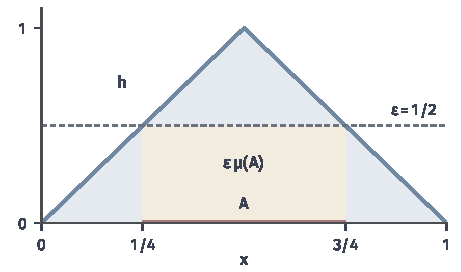
\includegraphics[width=78mm]{figures/04-spaces-measures-and-geometry/03-function-spaces/matplotlib/nspace-chebyshev/figure.pdf}
  \caption{Chebyshev不等式，取$h(x)=1-\lvert2x-1\rvert$、$\varepsilon=\tfrac12$。红线是超差集合$A=(\tfrac14,\tfrac34)$，黄色矩形面积$\varepsilon\,\mu(A)=\tfrac14$，含于面积为$\lVert h\rVert_1=\tfrac12$的蓝色区域之内。}
  \label{fig:nspace-chebyshev}
\end{BookInlineFigure}

\paragraph{有限测度下几乎处处收敛推出依测度收敛}
几乎处处收敛说每一点（零测集之外）迟早进入误差带，依测度收敛说没进入误差带的区域在缩小。在有限测度空间中，前者推出后者。

\begin{theorem}[几乎处处收敛推出依测度收敛]
\label{thm:nspace-ae-to-measure}
设$\mu(X)<\infty$，$f_n\to f$几乎处处。则$f_n$依测度收敛到$f$。
\end{theorem}

\begin{proof}
固定$\varepsilon>0$，令
\[
 B_N=\bigcup_{n\geq N}\{\lvert f_n-f\rvert>\varepsilon\},
\]
它随$N$单调下降。若$x\in\bigcap_NB_N$，则有无穷多个$n$使$\lvert f_n(x)-f(x)\rvert>\varepsilon$，$f_n(x)$不收敛到$f(x)$。所以$\bigcap_NB_N$含于不收敛点的集合，是零测集。

$\mu(B_1)\leq\mu(X)<\infty$，由测度的上连续性，
\[
 \mu(B_N)\to\mu\Bigl(\bigcap_NB_N\Bigr)=0.
\]
而$\{\lvert f_N-f\rvert>\varepsilon\}\subseteq B_N$，所以它的测度也趋于零。
\end{proof}

上连续性要求$\mu(B_1)<\infty$，有限测度正是用在这里。测度无限时结论失败：在$\mathbb R$上取Lebesgue测度与$f_n=\mathbf 1_{[n,n+1]}$，每一点在$n>x$后都有$f_n(x)=0$，处处收敛到$0$；但$\mu(\{f_n>\tfrac12\})=1$，不依测度收敛。

\paragraph{依测度收敛列的几乎处处收敛子列}
依测度收敛推不出几乎处处收敛，打字机序列就是例子。但和$L^p$收敛一样，总可以抽出一个几乎处处收敛的子列。

\begin{theorem}[依测度收敛的子列]
\label{thm:nspace-measure-subsequence}
设$f_n$依测度收敛到$f$。则存在子列$(f_{n_k})$，使$f_{n_k}\to f$几乎处处。
\end{theorem}

\begin{proof}
由定义，可以递归地取$n_1<n_2<\cdots$，使$E_k=\{\lvert f_{n_k}-f\rvert>2^{-k}\}$满足$\mu(E_k)<2^{-k}$。令$F_j=\bigcup_{k\geq j}E_k$，则
\[
 \mu(F_j)\leq\sum_{k\geq j}2^{-k}=2^{1-j}.
\]
若$x\notin F_j$，则对所有$k\geq j$有$\lvert f_{n_k}(x)-f(x)\rvert\leq2^{-k}$，所以$f_{n_k}(x)\to f(x)$。

于是不收敛的点都落在$\bigcap_jF_j$中，而$\mu(\bigcap_jF_j)\leq\mu(F_j)\leq2^{1-j}$对每个$j$成立，这个集合是零测集。
\end{proof}

证明的想法是挑选超差集合测度可求和的子列，使“无穷多次超差”的点只能组成零测集。这里没有用到测度有限。结合Chebyshev不等式，它也给出了定理~\ref{thm:nspace-lp-ae-subsequence}的另一个证明。

\subsection{一致可积性}
\label{sec:nspace-uniform-integrability}

窄尖峰依测度收敛到$0$，$L^1$误差却恒为$1$：峰越来越窄，但越来越高，积分始终集中在测度趋零的区域上。要从依测度收敛得到$L^1$收敛，需要防止积分躲进小区域里的大取值中。第~\ref{chap:integration}章的支配收敛定理用一个共同的可积上界做到这一点；一致可积性是更弱、却恰好够用的条件。本小节设$\mu(X)<\infty$。

\begin{definition}[一致可积]
\label{def:nspace-uniform-integrability}
设$\mu(X)<\infty$，$\{f_n\}\subseteq L^1(\mu)$。若
\begin{equation}
 \lim_{M\to\infty}\ \sup_{n}\int_{\{\lvert f_n\rvert>M\}}\lvert f_n\rvert\,d\mu=0,
 \label{eq:nspace-uniform-integrability}
\end{equation}
称$\{f_n\}$\term{一致可积}（uniformly integrable）。
\end{definition}

对单个可积函数$f$，总有
\[
 \int_{\{\lvert f\rvert>M\}}\lvert f\rvert\,d\mu\to0\qquad(M\to\infty).
\]
这是因为被积函数$\lvert f\rvert\mathbf 1_{\{\lvert f\rvert>M\}}$被$\lvert f\rvert$控制，且在$\lvert f\rvert<\infty$的点处当$M\to\infty$时趋于零，由支配收敛定理即得。一致可积要求这件事对整族函数以同样的速度发生，即大取值区域上的积分一致地小。

\paragraph{尖峰与共同上界}
窄尖峰不是一致可积的。对任意$M$，当$n>M$时$\{g_n>M\}=(0,1/n)$，其上的积分为$1$，所以
\[
 \sup_n\int_{\{g_n>M\}}g_n\,d\mu=1
\]
不随$M$趋于零。这正是它不$L^1$收敛的原因。

把峰的高度从$n$压到$\sqrt n$，情况就变了。令$f_n=\sqrt n\,\mathbf 1_{(0,1/n)}$，只有$\sqrt n>M$时$\{f_n>M\}$才非空，其上的积分为
\[
 \int_{\{f_n>M\}}f_n\,d\mu=\sqrt n\cdot\frac1n=\frac1{\sqrt n}<\frac1M.
\]
上确界不超过$1/M$，所以这一族一致可积。图~\ref{fig:nspace-uniform-integrability}并排画出这两族函数。

\begin{BookInlineFigure}
  \centering
  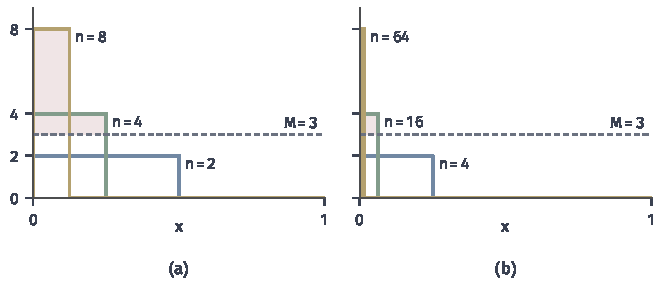
\includegraphics[width=112mm]{figures/04-spaces-measures-and-geometry/03-function-spaces/matplotlib/nspace-uniform-integrability/figure.pdf}
  \caption{尖峰的一致可积性，阈值$M=3$，浅红色为函数高于$M$的部分。(a)$g_n=n\mathbf 1_{(0,1/n)}$，$n=2,4,8$：每个高于阈值的尖峰，整根矩形的面积都是$1$，阈值抬高也不变。(b)$f_n=\sqrt n\,\mathbf 1_{(0,1/n)}$，$n=4,16,64$：高度相同的情况下宽度小得多，$\{f_n>M\}$上的积分是$1/\sqrt n$，随$n$变小。}
  \label{fig:nspace-uniform-integrability}
\end{BookInlineFigure}

有共同可积上界的族总是一致可积的。若$\lvert f_n\rvert\leq G$几乎处处对所有$n$成立，$G\in L^1$，则$\{\lvert f_n\rvert>M\}\subseteq\{G>M\}$，
\[
 \sup_n\int_{\{\lvert f_n\rvert>M\}}\lvert f_n\rvert\,d\mu\leq\int_{\{G>M\}}G\,d\mu\to0.
\]
窄尖峰没有这样的上界：$\sup_ng_n(x)$在$x\in[\tfrac1{n+1},\tfrac1n)$上等于$n>\tfrac1x-1$，不可积。

\paragraph{一致的小区域控制}
一致可积的族在小区域上的积分也一致地小，这是下面证明要用的形式。对任意可测集$A$与$M>0$，把$A$分成$\lvert f_n\rvert>M$与$\lvert f_n\rvert\leq M$两部分，得到
\begin{equation}
 \int_A\lvert f_n\rvert\,d\mu\leq\int_{\{\lvert f_n\rvert>M\}}\lvert f_n\rvert\,d\mu+M\mu(A).
 \label{eq:nspace-ui-small-sets}
\end{equation}

给定$\eta>0$，先取$M$使第一项对所有$n$都小于$\eta/2$，再令$\delta=\eta/(2M)$，则$\mu(A)<\delta$时$\sup_n\int_A\lvert f_n\rvert\,d\mu<\eta$。取$A=X$还得到$\sup_n\lVert f_n\rVert_1\leq\eta/2+M\mu(X)<\infty$，一致可积的族在$L^1$中有界。

\paragraph{从依测度收敛到\texorpdfstring{$L^1$}{L1}收敛}
有了小区域上的一致控制与$L^1$有界性，就可以把依测度收敛加强为$L^1$收敛：大误差区域的测度趋于零，一致可积保证这些区域上的积分也趋于零。

\begin{theorem}[依测度收敛与一致可积推出\texorpdfstring{$L^1$}{L1}收敛]
\label{thm:nspace-vitali}
设$\mu(X)<\infty$，$\{f_n\}\subseteq L^1(\mu)$一致可积，且$f_n$依测度收敛到可测函数$f$。则$f\in L^1(\mu)$，且$\lVert f_n-f\rVert_1\to0$。
\end{theorem}

\begin{proof}
先证$f$可积。由定理~\ref{thm:nspace-measure-subsequence}，有子列$f_{n_k}\to f$几乎处处。由Fatou引理与上面的$L^1$有界性，
\[
 \int_X\lvert f\rvert\,d\mu\leq\liminf_{k\to\infty}\int_X\lvert f_{n_k}\rvert\,d\mu\leq\sup_n\lVert f_n\rVert_1<\infty.
\]

再估计误差。给定$\varepsilon>0$与$\eta>0$，令$A_n=\{\lvert f_n-f\rvert>\varepsilon\}$。在$A_n$之外误差不超过$\varepsilon$，在$A_n$上用三角不等式，所以
\[
 \int_X\lvert f_n-f\rvert\,d\mu\leq\varepsilon\,\mu(X)+\int_{A_n}\lvert f_n\rvert\,d\mu+\int_{A_n}\lvert f\rvert\,d\mu.
\]

对族$\{f_n\}$取上一段的$\delta_1$；单个可积函数$f$构成的族$\{f\}$也一致可积，对它取$\delta_2$。依测度收敛给出$N$，使$n\geq N$时$\mu(A_n)<\min(\delta_1,\delta_2)$，此时后两项都小于$\eta$。于是$n\geq N$时
\[
 \lVert f_n-f\rVert_1\leq\varepsilon\,\mu(X)+2\eta.
\]
$\varepsilon,\eta$任意，故$\lVert f_n-f\rVert_1\to0$。
\end{proof}

证明把误差分成两部分：在误差不超过$\varepsilon$的区域上，贡献至多$\varepsilon\mu(X)$；误差超过$\varepsilon$的区域测度趋零，依测度收敛只保证这一点，其上的积分则由一致可积控制。有限测度用在两处：$\varepsilon\mu(X)$有限，以及式~\eqref{eq:nspace-ui-small-sets}给出$L^1$有界。

用前面的例子验证。$f_n=\sqrt n\,\mathbf 1_{(0,1/n)}$一致可积，又依测度收敛到$0$，定理给出$\lVert f_n\rVert_1\to0$；直接计算也得到$\lVert f_n\rVert_1=1/\sqrt n\to0$。窄尖峰不满足一致可积，定理不能用，结论也确实不成立。

\paragraph{回到支配收敛}
若$f_n\to f$几乎处处，且$\lvert f_n\rvert\leq G\in L^1$，则在有限测度下，定理~\ref{thm:nspace-ae-to-measure}给出依测度收敛，上面的论证给出一致可积，于是定理~\ref{thm:nspace-vitali}推出$\lVert f_n-f\rVert_1\to0$。这就回到了第~\ref{chap:integration}章的支配收敛定理。

共同可积上界只是一致可积的充分条件。一致可积只要求大取值区域上的积分一致地小，允许没有共同可积上界的族。

反过来，在有限测度下，$L^1$收敛的序列一定一致可积。证明要把前面的小区域控制转回大取值集合，篇幅较长，读者可查阅测度论的教材。所以在有限测度下，一致可积恰好刻画了依测度收敛何时能升级为$L^1$收敛。

\section{本章小结}
\label{sec:nspace-summary}

章首的问题是：比较两个函数时用哪一种误差，以及误差趋零的过程能否在空间内找到终点。范数回答前一个问题。它满足正定性、齐次性和三角不等式，诱导出距离、收敛和柯西列；最大绝对值看最坏位置，积分看总体累计，两者在$C[0,1]$上只有单向的控制$\lVert f\rVert_1\leq\lVert f\rVert_\infty$。有限维中任意两个范数等价，无限维中则不然：借助第~\ref{chap:functions-as-vectors}章两两远离的单位列和一组代数基，可以在任何无限维赋范空间上造出不等价的范数，$x^n$则在$C[0,1]$上给出具体例子。所以无限维中的收敛必须连同范数一起陈述。

完备性回答后一个问题。Banach空间中每个柯西列都有极限；Banach空间的线性子空间完备当且仅当它是闭集，多项式在最大误差下就不闭。紧集上的连续函数在一致范数下完备，证明依靠一致柯西列的极限与一致极限的连续性；非紧定义域上改用有界连续函数，只需补上极限的有界性。同一个$C[0,1]$在积分范数下不完备，逼近阶跃函数的折线列没有连续的极限。

$L^p$与$L^\infty$为积分误差下的极限提供了去处。它们的元素是几乎处处相等的可测函数组成的等价类，因而一般没有点值；计数测度下得到数列空间$\ell^p$与$\ell^\infty$。$L^p$的三角不等式来自Young、Hölder与Minkowski不等式，完备性的证明先抽相邻误差可求和的子列，再用Fatou引理回到积分。$L^\infty$用本质上确界忽略零测集，Hölder不等式在端点$p=1$、$q=\infty$同样成立，完备性来自把可数个例外集合并成一个零测集后的一致收敛。

各种收敛方式控制的误差不同。一致收敛推出$L^p$收敛需要有限测度；逐点收敛管不住窄尖峰，$L^p$收敛推不出逐点收敛，打字机序列是例子；但$L^p$收敛与依测度收敛的序列都有几乎处处收敛的子列。依测度收敛只控制大误差出现的范围，在有限测度下配合一致可积性才推出$L^1$收敛，共同可积上界是一致可积的充分条件，由此回到支配收敛定理。

本章只在单个空间内比较误差。内积带来的正交结构与最佳逼近在第~\ref{chap:inner-product-spaces}章研究；把一个空间放进另一个空间时误差怎样传递，即包含映射的有界性，在第~\ref{chap:linear-operators}章研究；用简单函数、连续函数逼近$L^p$中的元素，在第~\ref{chap:function-approximation}章研究。


\chapter{内积空间}
\label{chap:inner-product-spaces}

在$[-1,1]$上用常数近似$x^2$，最好的常数是多少？若用平方积分衡量误差，答案是$x^2$的平均值$\tfrac13$，误差函数$x^2-\tfrac13$与所有常数“垂直”。再问用$1,x,x^2,\ldots$的组合近似一个阶跃函数，项数越多误差是否越小、能否趋于零？这类问题需要的不只是误差的大小，还需要两个函数之间的角度。上一章的范数只提供前者，本章加入内积，研究正交带来的最佳逼近与无限展开。

本章先建立结构，再研究几何。第~\ref{sec:ipspace-inner-products}节把卷二的内积推广到函数与数列，固定实、复两种情形的约定，并说明内积怎样诱导范数、哪些范数不来自内积。第~\ref{sec:ipspace-hilbert-spaces}节把完备的内积空间称为Hilbert空间，第~\ref{sec:ipspace-l2-space}节以$L^2$与$\ell^2$说明内积、范数与完备性怎样同时成立。

后三节研究正交几何。第~\ref{sec:ipspace-orthogonal-projection}节证明Hilbert空间中闭子空间上的最佳逼近存在且唯一，它就是正交投影；这里完备性和闭性各有分工。第~\ref{sec:ipspace-orthonormal-bases}节定义完备正交系，说明它与代数基的区别，以及可分空间为什么有可数的正交基。第~\ref{sec:ipspace-orthogonal-expansions}节用正交系的系数写出展开，证明Bessel不等式与Parseval等式，并给出截断误差。

本章只研究内积带来的几何结构。连续线性泛函怎样表示为内积、正交投影作为算子的性质，分别在第~\ref{chap:linear-functionals}章和第~\ref{chap:linear-operators}章研究；三角函数系与小波的完备性在第~\ref{chap:fourier-transform}章和第~\ref{chap:wavelet-transform}章研究；正交展开的截断误差与函数光滑性的关系由第~\ref{chap:function-approximation}章处理；点值读取连续的Hilbert函数空间是第~\ref{chap:rkhs}章的对象。

\section{内积}
\label{sec:ipspace-inner-products}

\BookChapterRef{chap:inner-product-spaces}{卷二第4章“内积空间”}用内积定义了有限维空间中的长度、夹角和正交。内积的公理只涉及加法、数乘和取值，没有提到维数，所以可以原样放到函数和数列上。需要重新确认的是：函数上的内积具体长什么样，它给出的长度为什么是范数，以及哪些范数根本不可能来自内积。

\paragraph{内积的公理}
实空间中的内积是对称、双线性、正定的。复空间不能照搬这三条。若内积对两个变量都线性，把$x$换成$\mathrm ix$就得到
\[
 \langle\mathrm ix,\mathrm ix\rangle=\mathrm i^2\langle x,x\rangle=-\langle x,x\rangle,
\]
于是$\langle x,x\rangle$与$\langle\mathrm ix,\mathrm ix\rangle$不可能都是正数。所以复内积改用共轭对称，并且只对一个变量线性。本书与卷二一致，约定对第二个变量线性、对第一个变量共轭线性。

\begin{definition}[内积与内积空间]
\label{def:ipspace-inner-product}
设$V$是$\mathbb K$上的线性空间。映射$\langle\cdot,\cdot\rangle:V\times V\to\mathbb K$称为$V$上的\term{内积}（inner product），若对所有$f,g,h\in V$与$a,b\in\mathbb K$，
\begin{align}
 \langle h,af+bg\rangle&=a\langle h,f\rangle+b\langle h,g\rangle,
 \label{eq:ipspace-axiom-linear}\\
 \langle g,f\rangle&=\overline{\langle f,g\rangle},
 \label{eq:ipspace-axiom-conjugate}\\
 \langle f,f\rangle&\geq0,
 \label{eq:ipspace-axiom-positive}
\end{align}
且$\langle f,f\rangle=0$当且仅当$f=0$。这三条分别称为对第二个变量线性、共轭对称和正定性。配备内积的线性空间称为\term{内积空间}（inner-product space）。
\end{definition}

前两条合起来给出对第一个变量的共轭线性：
\[
 \langle af+bg,h\rangle=\bar a\langle f,h\rangle+\bar b\langle g,h\rangle.
\]
共轭对称还说明$\langle f,f\rangle$等于自己的共轭，总是实数，所以第三条的“$\geq0$”有意义。实空间中共轭不起作用，三条公理就是卷二的对称、双线性和正定性。

\paragraph{函数与数列上的内积}
先看点积怎样变成积分。把$[-1,1]$等分成$N$小段，步长$h=2/N$，取各段中点$x_1,\ldots,x_N$。函数$f$在这些点上读出一个$N$维向量$(f(x_1),\ldots,f(x_N))$，这正是“函数是无限维向量”的有限截取。两个这样的向量作点积，再乘以步长，得到
\begin{equation}
 h\sum_{i=1}^N\overline{f(x_i)}\,g(x_i)\ \xrightarrow{\ N\to\infty\ }\ \int_{-1}^1\overline{f(x)}\,g(x)\,dx .
 \label{eq:ipspace-riemann-dot}
\end{equation}
乘以$h$是必要的：不乘的话，分量越多点积越大，没有极限。

下面用$f(x)=1+x$、$g(x)=x$和$N=4$算一遍。此时$h=\tfrac12$，四个中点是$\pm\tfrac14,\pm\tfrac34$，两个函数读出的向量是
\[
 f\mapsto(0.25,\,0.75,\,1.25,\,1.75),\qquad g\mapsto(-0.75,\,-0.25,\,0.25,\,0.75).
\]
逐分量相乘再相加，得到点积
\[
 -0.1875-0.1875+0.3125+1.3125=1.25 .
\]
乘以步长$h=\tfrac12$，得到$0.625$。

精确的积分是
\[
 \int_{-1}^1(1+x)x\,dx=\int_{-1}^1x\,dx+\int_{-1}^1x^2\,dx=\frac23 .
\]
取$N=8$和$N=16$，同样的计算分别给出$0.65625$和$0.6640625$，逐渐接近$\tfrac23$。图~\ref{fig:ipspace-sampled-dot-product}画出了$N=4$时的情形：左边是两组读出的分量，右边每个矩形的高是一对分量的乘积，矩形的带符号总面积就是式~\eqref{eq:ipspace-riemann-dot}左边的和。

\begin{BookInlineFigure}
  \centering
  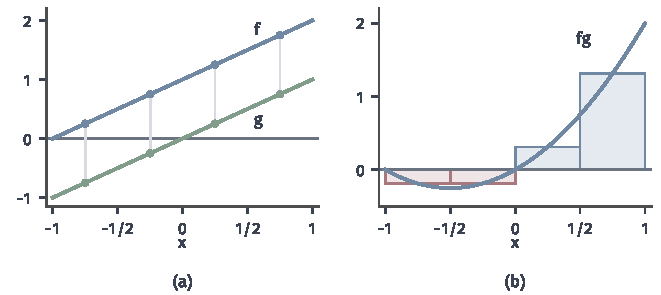
\includegraphics[width=112mm]{figures/04-spaces-measures-and-geometry/03-function-spaces/matplotlib/ipspace-sampled-dot-product/figure.pdf}
  \caption{从点积到积分内积，$f=1+x$（蓝），$g=x$（绿），$N=4$。(a)四个中点上读出的分量。(b)矩形的高是分量的乘积$f(x_i)g(x_i)$（负值用红色），宽是步长$\tfrac12$，带符号总面积$0.625$；曲线是$fg$，其下带符号面积是内积$\tfrac23$。}
  \label{fig:ipspace-sampled-dot-product}
\end{BookInlineFigure}

这个极限提示了$C[a,b]$上的内积：
\begin{equation}
 \langle f,g\rangle=\int_a^b\overline{f(x)}\,g(x)\,dx .
 \label{eq:ipspace-continuous-inner-product}
\end{equation}
实函数时共轭可以省去。对第二个变量的线性和共轭对称来自积分的线性。

正定性要用到连续性。被积函数非负，所以
\[
 \langle f,f\rangle=\int_a^b\lvert f\rvert^2\,dx\geq0 .
\]
若$f(x_0)\neq0$，由连续性存在长度为正的小区间，在其上$\lvert f\rvert\geq\tfrac12\lvert f(x_0)\rvert$，积分至少是区间长度乘$\tfrac14\lvert f(x_0)\rvert^2$，严格为正。

这里类比也开始失效。有限维向量的每个分量都带着正的权重，改动一个分量，长度就变了。积分内积中单个点的权重趋于零，改动一个点的值不影响积分。在连续函数上，连续性阻止了这种改动；一旦离开连续函数，正定性就要靠第~\ref{sec:ipspace-l2-space}节的等价类来恢复。

数列是更直接的无限维向量，下标集是$\mathbb N_+$，内积就是点积把求和号延伸到无穷：$\sum_k\overline{x_k}y_k$。麻烦在于和可能发散，比如$(1,1,1,\ldots)$与自己的点积。在有限支撑数列空间$c_{00}$上不会有这个问题，求和只有有限项非零，
\begin{equation}
 \langle x,y\rangle=\sum_k\overline{x_k}\,y_k
 \label{eq:ipspace-c00-inner-product}
\end{equation}
是内积。容纳无穷多项非零的数列要等到第~\ref{sec:ipspace-l2-space}节的$\ell^2$。

共轭在函数上同样不能省略。在$[-\pi,\pi]$上取$f(x)=e^{\mathrm ix}$，这是一个处处模长为$1$的非零函数。若不取共轭，
\[
 \int_{-\pi}^{\pi}f(x)\,f(x)\,dx=\int_{-\pi}^{\pi}e^{2\mathrm ix}\,dx=0,
\]
一个非零函数与自己的“内积”竟然为零。取共轭后被积函数变成$\lvert e^{\mathrm ix}\rvert^2=1$，于是$\langle f,f\rangle=2\pi$。

若$\langle f,g\rangle=0$，称$f$与$g$\term{正交}（orthogonal）。这里的“垂直”指乘积的整体积分为零，与两条曲线在平面上的交角无关。在$[-1,1]$上，$1$与$x$正交，$1$与$x^2$不正交，因为
\[
 \int_{-1}^1x\,dx=0,\qquad \int_{-1}^1x^2\,dx=\frac23 .
\]
正交还依赖积分区间：换到$[0,1]$上，$\int_0^1x\,dx=\tfrac12$，$1$与$x$就不再正交了。

\paragraph{Cauchy--Schwarz不等式与诱导范数}
内积给出长度$\lVert f\rVert=\sqrt{\langle f,f\rangle}$。要说明它是范数，关键在三角不等式，而三角不等式依赖下面这个不等式。

它的几何图景是：$\mathbb R^3$中把$f$投影到$g$所在的直线上，垂线段的长度不小于零，由此得到$\cos\theta$的绝对值不超过$1$。证明就是把这幅图写成计算，用到的只有内积公理，与维数无关。

\begin{theorem}[Cauchy--Schwarz不等式]
\label{thm:ipspace-cauchy-schwarz}
在内积空间中，对所有$f,g$，
\begin{equation}
 \lvert\langle f,g\rangle\rvert\leq\lVert f\rVert\,\lVert g\rVert ,
 \label{eq:ipspace-cauchy-schwarz}
\end{equation}
等号当且仅当$f,g$线性相关。
\end{theorem}

\begin{proof}
若$g=0$，两边都为零，$f,g$线性相关。下面设$g\neq0$。

取$f$在$g$方向上的影子$\alpha g$，其中$\alpha=\langle g,f\rangle/\lVert g\rVert^2$。这个系数使余量$f-\alpha g$与$g$正交：
\[
 \langle g,f-\alpha g\rangle=\langle g,f\rangle-\alpha\lVert g\rVert^2=0 .
\]

展开余量长度的平方时，先把第二个变量拆开。含$g$的那一项因为上面的正交关系而消失，于是
\[
 \lVert f-\alpha g\rVert^2=\langle f-\alpha g,f\rangle=\lVert f\rVert^2-\bar\alpha\langle g,f\rangle .
\]

代入$\bar\alpha=\langle f,g\rangle/\lVert g\rVert^2$。$\langle f,g\rangle$与$\langle g,f\rangle$互为共轭，乘积是模的平方，于是
\[
 0\leq\lVert f-\alpha g\rVert^2=\lVert f\rVert^2-\frac{\lvert\langle f,g\rangle\rvert^2}{\lVert g\rVert^2}.
\]
移项开方即得不等式。等号成立当且仅当$\lVert f-\alpha g\rVert=0$，即$f=\alpha g$；反过来，若$f=cg$，直接代入可知$\alpha=c$，等号成立。
\end{proof}

用$[0,1]$上的$f=1$、$g=x$核对一下。三个内积是
\[
 \langle f,g\rangle=\frac12,\qquad \lVert f\rVert^2=1,\qquad \lVert g\rVert^2=\frac13 .
\]
不等式成为$\tfrac12\leq\tfrac1{\sqrt3}\approx0.577$。影子的系数是$\alpha=\tfrac12\big/\tfrac13=\tfrac32$，余量$1-\tfrac32x$的长度平方是
\[
 \int_0^1\Bigl(1-\frac32x\Bigr)^2dx=1-\frac32+\frac34=\frac14,
\]
与证明中的公式给出的$1-\tfrac34$相同。

在实空间中，式~\eqref{eq:ipspace-cauchy-schwarz}保证下面的比值落在$[-1,1]$内，可以用它定义函数之间的夹角：
\[
 \cos\theta=\frac{\langle f,g\rangle}{\lVert f\rVert\,\lVert g\rVert}.
\]
上面的$1$与$x$在$[0,1]$上的夹角满足$\cos\theta=\tfrac{\sqrt3}2$，即$\theta=30^\circ$；在$[-1,1]$上内积为零，夹角是$90^\circ$。

三角不等式现在可以推出。把$\lVert f+g\rVert^2$按内积展开，再用Cauchy--Schwarz不等式放大交叉项：
\[
 \begin{aligned}
 \lVert f+g\rVert^2&=\lVert f\rVert^2+2\operatorname{Re}\langle f,g\rangle+\lVert g\rVert^2\\
 &\leq\lVert f\rVert^2+2\lVert f\rVert\,\lVert g\rVert+\lVert g\rVert^2\\
 &=(\lVert f\rVert+\lVert g\rVert)^2 .
 \end{aligned}
\]
齐次性$\lVert cf\rVert=\lvert c\rvert\,\lVert f\rVert$与正定性直接来自内积公理。所以每个内积空间都是赋范空间，这个范数称为内积的\term{诱导范数}（induced norm）。在$C[a,b]$上，它就是平方积分大小$\bigl(\int_a^b\lvert f\rvert^2\,dx\bigr)^{1/2}$。

Cauchy--Schwarz不等式还说明内积对两个变量连续。把差拆成只改一个变量的两项：
\[
 \langle f_n,g_n\rangle-\langle f,g\rangle=\langle f_n-f,g_n\rangle+\langle f,g_n-g\rangle .
\]
对每一项用不等式~\eqref{eq:ipspace-cauchy-schwarz}，得到
\begin{equation}
 \lvert\langle f_n,g_n\rangle-\langle f,g\rangle\rvert\leq\lVert f_n-f\rVert\,\lVert g_n\rVert+\lVert f\rVert\,\lVert g_n-g\rVert .
 \label{eq:ipspace-inner-continuity}
\end{equation}
若$f_n\to f$、$g_n\to g$，$\lVert g_n\rVert$有界，右边趋于零，所以$\langle f_n,g_n\rangle\to\langle f,g\rangle$。后面凡是在极限中保持正交关系，用的都是这一点。

\paragraph{平行四边形恒等式}
内积范数比一般范数多一条性质。在平面上，平行四边形两条对角线的平方和等于四条边的平方和。这条几何事实在内积空间中照样成立：
\begin{equation}
 \lVert f+g\rVert^2+\lVert f-g\rVert^2=2\lVert f\rVert^2+2\lVert g\rVert^2 ,
 \label{eq:ipspace-parallelogram}
\end{equation}
称为\term{平行四边形恒等式}（parallelogram identity）。验证时把左边两项按内积展开，交叉项$2\operatorname{Re}\langle f,g\rangle$与$-2\operatorname{Re}\langle f,g\rangle$相互抵消，剩下的正是右边。

一般的范数未必满足它，因此未必来自内积。在$C[0,1]$上取一致范数，令$f=1$、$g=x$。这时$f+g=1+x$的最大值是$2$，$f-g=1-x$的最大值是$1$，于是
\[
 \lVert f+g\rVert_\infty^2+\lVert f-g\rVert_\infty^2=4+1=5 .
\]
而$\lVert f\rVert_\infty=\lVert g\rVert_\infty=1$，右边是
\[
 2\lVert f\rVert_\infty^2+2\lVert g\rVert_\infty^2=4 .
\]

$L^1$范数同样不满足。在$L^1[0,1]$中取两半区间的指示函数$f=\mathbf 1_{[0,1/2]}$、$g=\mathbf 1_{(1/2,1]}$，有
\[
 \lVert f+g\rVert_1=\lVert f-g\rVert_1=1,\qquad \lVert f\rVert_1=\lVert g\rVert_1=\frac12 .
\]
左边等于$2$，右边等于$1$。两个范数都违反式~\eqref{eq:ipspace-parallelogram}，所以没有任何内积能诱导它们。

反过来，满足平行四边形恒等式的范数一定来自内积。实情形下这个内积只能是
\begin{equation}
 \langle f,g\rangle=\frac14\bigl(\lVert f+g\rVert^2-\lVert f-g\rVert^2\bigr) ,
 \label{eq:ipspace-polarization}
\end{equation}
因为按内积展开右边，正好只剩$\langle f,g\rangle$。证明这个式子确实定义了内积，需要由恒等式逐步推出可加性，再把齐次性从有理数推广到实数，篇幅较长，读者可在泛函分析教材中查阅Jordan--von Neumann定理。本章只用正方向：内积范数满足式~\eqref{eq:ipspace-parallelogram}，它将是第~\ref{sec:ipspace-orthogonal-projection}节证明最近点存在的关键。

\section{Hilbert空间}
\label{sec:ipspace-hilbert-spaces}

内积空间是赋范空间，因而可以谈柯西列与完备性。下一节之后的最佳逼近与无限展开都要从柯西列得到极限，所以需要把完备性与内积放在一起。

\begin{definition}[Hilbert空间]
\label{def:ipspace-hilbert}
若内积空间在诱导范数下完备，即诱导度量满足第~\ref{chap:metric-spaces}章的完备性，称它为\term{Hilbert空间}（Hilbert space）。
\end{definition}

按定义，Hilbert空间就是范数来自内积的Banach空间。反过来不成立：上一节说明一致范数与$L^1$范数不满足平行四边形恒等式，而第~\ref{chap:normed-spaces}章证明了$C[0,1]$在一致范数下完备、$L^1[0,1]$完备，所以它们是Banach空间，却不是Hilbert空间。“有没有内积”和“是否完备”是两个独立的判断。

有限维内积空间总是完备的，因为有限维赋范空间在任意范数下都完备。所以有限维时，内积空间与Hilbert空间是同一回事，卷二的全部正交理论都在完备空间中进行。无限维时，完备性要对每个具体空间单独证明；下面两个例子说明它确实可能不成立。

\paragraph{有限支撑数列}
在$c_{00}$上取内积$\langle x,y\rangle=\sum_k\overline{x_k}y_k$。令
\begin{equation*}
x^{(N)}=(1,\tfrac12,\ldots,\tfrac1N,0,0,\ldots)\in c_{00}.
\end{equation*}
对$M>N$，
\[
 \lVert x^{(M)}-x^{(N)}\rVert^2=\sum_{k=N+1}^M\frac1{k^2}\leq\sum_{k>N}\frac1{k^2}\to0,
\]
所以$(x^{(N)})$是柯西列。

它在$c_{00}$中没有极限。若$\lVert x^{(N)}-y\rVert\to0$对某个$y\in c_{00}$成立，由于每个坐标的差都不超过范数，$\lvert x^{(N)}_k-y_k\rvert\leq\lVert x^{(N)}-y\rVert$，每个坐标都收敛，所以$y_k=\lim_Nx^{(N)}_k=1/k$对所有$k$成立。这样的$y$有无穷多项非零，不在$c_{00}$中，矛盾。所以$c_{00}$是不完备的内积空间。

\paragraph{连续函数与平方积分}
在$C[-1,1]$上取实内积$\langle f,g\rangle=\int_{-1}^1fg\,dx$，诱导范数记为$\lVert\cdot\rVert_2$。连续斜坡
\[
 g_n(x)=\begin{cases}-1,&x\leq-1/n,\\ nx,&\lvert x\rvert<1/n,\\ 1,&x\geq1/n\end{cases}
\]
越来越陡，越来越像符号函数$\operatorname{sgn}$，如图~\ref{fig:ipspace-ramp-step}所示。对$m>n$，两函数只在$\lvert x\rvert<1/n$上不同且差的绝对值不超过$1$，所以$\lVert g_n-g_m\rVert_2^2\leq2/n$，$(g_n)$是柯西列。

\begin{figure}[!htb]
  \centering
  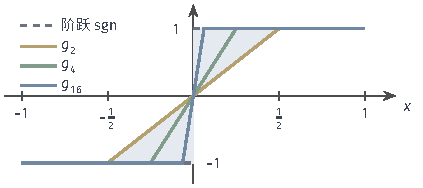
\includegraphics[width=71.6mm]{figures/02-abstract-mathematics/03-function-spaces/tikz/c1-ramp-step/figure.pdf}
  \caption{连续斜坡$g_n$逼近符号函数$\operatorname{sgn}$。$g_n$在$\lvert x\rvert\geq1/n$处与$\operatorname{sgn}$相同，只在宽为$2/n$的区间内线性过渡；阴影是$n=2$时二者之差所在的区域。直接积分得$\int_{-1}^1(g_n-\operatorname{sgn})^2\,dx=\tfrac{2}{3n}\to0$，但$\operatorname{sgn}$在$0$处跳跃，没有连续代表。}
  \label{fig:ipspace-ramp-step}
\end{figure}

它在$C[-1,1]$中没有$\lVert\cdot\rVert_2$极限。若连续函数$g$满足$\lVert g_n-g\rVert_2\to0$，任取$\delta\in(0,1)$，当$n>1/\delta$时$g_n$在$[\delta,1]$上恒为$1$，于是$\int_\delta^1(1-g)^2\,dx\leq\lVert g_n-g\rVert_2^2\to0$，由连续性$g=1$在$[\delta,1]$上成立；同理$g=-1$在$[-1,-\delta]$上成立。$\delta$任意，$g$在$0$处不可能连续，矛盾。这与第~\ref{chap:normed-spaces}章积分范数下的不完备例子是同一机制，只是误差改用平方累计。

两个例子中，柯西列的“极限”都存在，只是不在原来的集合里：前者是平方可和的数列$(1/k)$，后者是平方可积的阶跃函数。下一节的$\ell^2$与$L^2$正是把这些极限都收进来的空间。

\section{\texorpdfstring{$L^2$}{L2}空间}
\label{sec:ipspace-l2-space}

上一节的两个不完备例子分别缺少平方可和的数列和平方可积的阶跃函数。第~\ref{chap:function-normed-spaces}章已经在几乎处处等价类上建立了$L^2$，并证明它在$L^2$范数下完备。接下来只需在$L^2$上定义内积，并核对它诱导的正是这个范数。本节固定测度空间$(X,\mathcal A,\mu)$。

\paragraph{\texorpdfstring{$L^2$}{L2}内积}
点积推广到函数时写成乘积的积分，首先要保证这个积分有意义。有限维的和总是有限的，无限维时要靠条件。对$f,g\in L^2(\mu)$，Hölder不等式在$p=q=2$时给出
\[
 \int_X\lvert\bar fg\rvert\,d\mu=\int_X\lvert f\rvert\,\lvert g\rvert\,d\mu\leq\lVert f\rVert_2\,\lVert g\rVert_2<\infty,
\]
所以$\bar fg$可积。

于是可以令
\begin{equation}
 \langle f,g\rangle=\int_X\bar fg\,d\mu ,
 \label{eq:ipspace-l2-inner-product}
\end{equation}
实函数时共轭可以省去。复值函数的积分按第~\ref{chap:integration}章的规定，实部、虚部分别积分。

这个定义不依赖代表的选择。若$f'\sim_\mu f$、$g'\sim_\mu g$，则$\bar f'g'$与$\bar fg$只在零测集$\{f'\neq f\}\cup\{g'\neq g\}$上可能不同，积分相同。所以$\langle\cdot,\cdot\rangle$是等价类上定义合理的映射。

\paragraph{内积公理与诱导范数}
对第二个变量的线性来自积分的线性，共轭对称来自$\overline{\int\bar fg\,d\mu}=\int f\bar g\,d\mu$。正定性值得细看：被积函数非负，所以
\[
 \langle f,f\rangle=\int_X\lvert f\rvert^2\,d\mu\geq0 ,
\]
且它为零当且仅当$\lvert f\rvert^2=0$几乎处处，也就是$[f]$是零元素。

正是等价类使正定性成立。若在普通函数上计算，只在一点非零的函数也会使$\langle f,f\rangle=0$，正定性就失败了。第~\ref{sec:ipspace-inner-products}节说过，积分内积中单个点没有权重；把函数换成等价类，就是承认这件事，不再区分只差一个零测集的函数。

诱导范数是
\[
 \sqrt{\langle f,f\rangle}=\Bigl(\int_X\lvert f\rvert^2\,d\mu\Bigr)^{1/2}=\lVert f\rVert_2 ,
\]
恰好是第~\ref{chap:function-normed-spaces}章的$L^2$范数。那里已经证明$L^2(\mu)$在这个范数下完备，所以下面的定理不需要新的论证。

\begin{theorem}[$L^2$是Hilbert空间]
\label{thm:ipspace-l2-hilbert}
对任意测度空间，$L^2(\mu)$配以式~\eqref{eq:ipspace-l2-inner-product}的内积是Hilbert空间。
\end{theorem}

上一节的阶跃例子在这里有了去处。$\operatorname{sgn}$的等价类属于$L^2[-1,1]$。$g_n$与$\operatorname{sgn}$只在$\lvert x\rvert<1/n$上不同，左右两半对称，所以
\[
 \lVert g_n-\operatorname{sgn}\rVert_2^2=2\int_0^{1/n}(1-nx)^2\,dx=\frac{2}{3n}\to0 .
\]
斜坡列在$L^2[-1,1]$中收敛到$\operatorname{sgn}$。

\paragraph{\texorpdfstring{$\ell^2$}{l2}空间}
取$X=\mathbb N_+$与计数测度，积分变成求和，等价类就是数列本身，得到
\begin{equation}
 \begin{gathered}
 \ell^2=\Bigl\{x=(x_k):\ \sum_{k\geq1}\lvert x_k\rvert^2<\infty\Bigr\},\\
 \langle x,y\rangle=\sum_{k\geq1}\overline{x_k}\,y_k .
 \end{gathered}
 \label{eq:ipspace-ell2}
\end{equation}
这是最字面意义上的“无限维向量空间”：元素就是$[a_1,a_2,\ldots]$，内积就是点积，唯一的新要求是长度有限。级数的绝对收敛来自计数测度下的Hölder不等式。由定理~\ref{thm:ipspace-l2-hilbert}，$\ell^2$是Hilbert空间。

$c_{00}$是$\ell^2$的子空间，内积是限制后的内积，上一节的柯西列$x^{(N)}$在$\ell^2$中收敛到$(1/k)$。$c_{00}$的不完备，只是因为它没有包含这些极限。有限维的$\mathbb K^d$可以看作只有前$d$项非零的数列，这时$\ell^2$内积就是卷二的标准内积。

$\ell^2$与$L^2[-1,1]$的差别值得留意。两者都是Hilbert空间，但$\ell^2$的下标是离散的，每个坐标都带着权重$1$，读取第$k$个坐标是连续的操作；$L^2[-1,1]$中单点没有权重，读取函数在某一点的值根本没有定义。

\paragraph{\texorpdfstring{$L^2$}{L2}中的正交}
函数的正交是乘积的积分为零。图~\ref{fig:ipspace-integral-orthogonality}在$L^2[-1,1]$中对照了两种情形：$1\cdot x$在正负半区间上的带符号面积相互抵消；$1\cdot x^2$处处非负，面积无处抵消。同样的对称性说明，$[-1,1]$上任何偶函数都与任何奇函数正交，因为乘积是奇函数，积分为零。

\begin{BookInlineFigure}
  \centering
  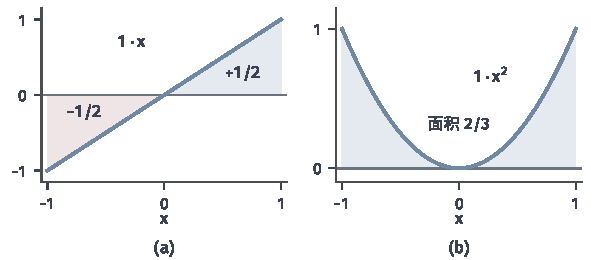
\includegraphics[width=100mm]{figures/04-spaces-measures-and-geometry/03-function-spaces/matplotlib/ipspace-integral-orthogonality/figure.pdf}
  \caption{积分内积下的正交。$[-1,1]$上取Lebesgue测度，曲线是两个函数的乘积，阴影是带符号面积。(a)$1\cdot x$的正负面积各为$\tfrac12$，内积为$0$，$1$与$x$正交。(b)$1\cdot x^2$处处非负，内积为$\tfrac23$，$1$与$x^2$不正交。}
  \label{fig:ipspace-integral-orthogonality}
\end{BookInlineFigure}

复情形的典型例子是复指数。在$L^2[-\pi,\pi]$中，对整数$j,k$，第一个变量取共轭，指数相减：
\[
 \begin{aligned}
 \langle e^{\mathrm ijx},e^{\mathrm ikx}\rangle
 &=\int_{-\pi}^{\pi}e^{-\mathrm ijx}e^{\mathrm ikx}\,dx\\
 &=\int_{-\pi}^{\pi}e^{\mathrm i(k-j)x}\,dx .
 \end{aligned}
\]
当$j=k$时被积函数为$1$，积分为$2\pi$。当$j\neq k$时，$e^{\mathrm imx}$（$m=k-j\neq0$）在一个周期上积分为零，因为它的原函数$e^{\mathrm imx}/(\mathrm im)$在两端取值相同。

所以$\{e^{\mathrm ikx}/\sqrt{2\pi}\}_{k\in\mathbb Z}$两两正交且长度为$1$。这一族是否足以表示$L^2[-\pi,\pi]$的每个元素，是第~\ref{chap:fourier-transform}章的问题。

\section{正交投影}
\label{sec:ipspace-orthogonal-projection}

章首问：在$L^2[-1,1]$中用常数近似$x^2$，哪个常数最好？更一般地，给定Hilbert空间$H$中的一个子空间$M$与一个目标$f$，能否在$M$中找到离$f$最近的元素。有限维中，卷二证明了最近点存在、唯一，并且误差与子空间正交。无限维中新的问题是：逼近距离的下确界能否被取到。本节证明，只要$H$完备、$M$闭，答案就是肯定的。

\paragraph{正交补}
先给出“与整个子空间垂直”的元素组成的集合。对子集$M\subseteq H$，令
\[
 M^\perp=\{g\in H:\ \langle m,g\rangle=0\ \text{对所有}\ m\in M\},
\]
称为$M$的\term{正交补}（orthogonal complement）。它是线性子空间，因为内积对第二个变量线性。它还是闭集：若$g_n\in M^\perp$且$g_n\to g$，由内积的连续性，$\langle m,g\rangle=\lim_n\langle m,g_n\rangle=0$对每个$m\in M$成立。所以无论$M$本身是否闭，$M^\perp$总是闭线性子空间。

\paragraph{最佳逼近的存在与唯一}
设$M\subseteq H$是线性子空间，$f\in H$，记
\[
 d=d(f,M)=\inf_{m\in M}\lVert f-m\rVert .
\]
下确界总是存在的。问题在于是否有$m\in M$恰好取到它：在无限维中，越来越好的近似可能没有极限，极限也可能离开$M$。下面的定理说明，完备性和闭性分别排除这两种情况，而平行四边形恒等式保证越来越好的近似确实彼此接近。

\begin{theorem}[闭子空间上的最佳逼近]
\label{thm:ipspace-best-approximation}
设$H$是Hilbert空间，$M\subseteq H$是闭线性子空间。则对每个$f\in H$，存在唯一的$m_*\in M$使$\lVert f-m_*\rVert=d(f,M)$。
\end{theorem}

\begin{proof}
取$m_n\in M$使$\lVert f-m_n\rVert^2<d^2+1/n$，称为极小化序列。

第一步，极小化序列是柯西列。对$f-m_j$与$f-m_k$用平行四边形恒等式~\eqref{eq:ipspace-parallelogram}，
\[
 \lVert m_j-m_k\rVert^2=2\lVert f-m_j\rVert^2+2\lVert f-m_k\rVert^2-4\Bigl\lVert f-\frac{m_j+m_k}2\Bigr\rVert^2 .
\]
$M$是线性子空间，中点$\tfrac{m_j+m_k}2$在$M$中，所以最后一项中的范数平方至少为$d^2$。于是$\lVert m_j-m_k\rVert^2<2(d^2+\tfrac1j)+2(d^2+\tfrac1k)-4d^2=\tfrac2j+\tfrac2k$，$(m_n)$是柯西列。

第二步，极限存在且留在$M$中。$H$完备，所以$m_n$收敛到某个$m_*\in H$；$M$闭，所以$m_*\in M$。由范数的连续性，$\lVert f-m_*\rVert=\lim_n\lVert f-m_n\rVert=d$。

第三步，唯一性。若$m_*,m_*'\in M$都取到$d$，则二者交替排列成的序列$m_*,m_*',m_*,m_*',\ldots$也是极小化序列，由第一步是柯西列，所以$m_*=m_*'$。
\end{proof}

三个条件各有分工。平行四边形恒等式说明：若两个点离$f$都几乎是最近的，它们彼此必然很近，这一步依赖内积，一般Banach空间中最近点可能不唯一，也可能不存在。$H$的完备性给出极小化序列的极限，$M$的闭性保证这个极限没有离开$M$。实际上前两步只用到$M$自身的完备性：若$M$在限制后的范数下完备，即使$H$不完备，结论也成立，这适用于任意内积空间中的有限维子空间。

\paragraph{误差正交与正交投影}
最近点还可以用正交关系刻画，这是计算它的实用方法。

\begin{theorem}[正交刻画]
\label{thm:ipspace-orthogonality-characterization}
设$H$是Hilbert空间，$M\subseteq H$是闭线性子空间，$f\in H$，$m_*\in M$。则$\lVert f-m_*\rVert=d(f,M)$当且仅当$f-m_*\in M^\perp$。此时对任意$m\in M$，
\begin{equation}
 \lVert f-m\rVert^2=\lVert f-m_*\rVert^2+\lVert m_*-m\rVert^2 .
 \label{eq:ipspace-pythagoras}
\end{equation}
\end{theorem}

\begin{proof}
设$m_*$取到$d$，记$r=f-m_*$。任取$m\in M$与$t\in\mathbb K$，$m_*+tm\in M$，所以$\lVert r\rVert^2\leq\lVert r-tm\rVert^2=\lVert r\rVert^2-2\operatorname{Re}\bigl(t\langle r,m\rangle\bigr)+\lvert t\rvert^2\lVert m\rVert^2$。取$t=s\,\overline{\langle r,m\rangle}$，$s>0$为实数，得$2s\lvert\langle r,m\rangle\rvert^2\leq s^2\lvert\langle r,m\rangle\rvert^2\lVert m\rVert^2$。两边除以$s$再令$s\to0$，得$\langle r,m\rangle=0$。所以$r\in M^\perp$。

反过来，设$r=f-m_*\in M^\perp$。对任意$m\in M$，$m_*-m\in M$与$r$正交，展开$\lVert r+(m_*-m)\rVert^2$时交叉项为零，得式~\eqref{eq:ipspace-pythagoras}。于是$\lVert f-m\rVert\geq\lVert f-m_*\rVert$，等号当且仅当$m=m_*$，$m_*$是最近点。
\end{proof}

式~\eqref{eq:ipspace-pythagoras}是勾股关系：$f$、$m_*$、$m$三点构成以$m_*$为直角顶点的直角三角形，见图~\ref{fig:ipspace-projection-geometry}。它不仅说明$m_*$最近，还定量地给出任何其他候选多出的误差，恰为它到$m_*$的距离平方。

\begin{figure}[!htb]
  \centering
  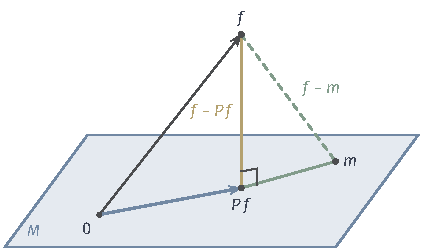
\includegraphics[width=71.7mm]{figures/02-abstract-mathematics/03-function-spaces/tikz/c1-projection-geometry/figure.pdf}
  \caption{闭子空间上的正交投影（示意）。平面代表闭子空间$M$，$Pf$是$M$中离$f$最近的点，误差$f-Pf$与$M$垂直。对$M$中任意另一点$m$，三点构成直角三角形，$\lVert f-m\rVert^2=\lVert f-Pf\rVert^2+\lVert Pf-m\rVert^2$，所以$m$离$f$更远。}
  \label{fig:ipspace-projection-geometry}
\end{figure}

\begin{definition}[正交投影]
\label{def:ipspace-orthogonal-projection}
设$M$是Hilbert空间$H$的闭线性子空间。把定理~\ref{thm:ipspace-best-approximation}中的最近点$m_*$记为$P_Mf$，称为$f$在$M$上的\term{正交投影}（orthogonal projection）。
\end{definition}

\paragraph{正交分解}
由定理~\ref{thm:ipspace-orthogonality-characterization}，每个$f\in H$都可以写成
\[
 f=P_Mf+(f-P_Mf),\qquad P_Mf\in M,\quad f-P_Mf\in M^\perp .
\]
这种分解是唯一的：若$f=m+g=m'+g'$，$m,m'\in M$，$g,g'\in M^\perp$，则$m-m'=g'-g$同时属于$M$与$M^\perp$，与自己正交，只能为零。所以$H$中每个元素唯一地分成$M$中的部分与$M^\perp$中的部分，记作$H=M\oplus M^\perp$。

由勾股关系还得到$\lVert f\rVert^2=\lVert P_Mf\rVert^2+\lVert f-P_Mf\rVert^2$，所以$\lVert P_Mf\rVert\leq\lVert f\rVert$。$P_M$的线性也可以从正交刻画读出：$af+bg-(aP_Mf+bP_Mg)$是两个$M^\perp$中元素的组合，仍在$M^\perp$中，所以$aP_Mf+bP_Mg$就是$af+bg$的投影。把$P_M$作为线性算子研究，是第~\ref{chap:linear-operators}章的内容。

\paragraph{向常数投影}
回到章首的问题。在$L^2[-1,1]$中取$M=\operatorname{span}\{1\}$，它是一维子空间，因而闭。由正交刻画，$c$是最佳常数当且仅当$\langle1,f-c\rangle=\int_{-1}^1(f-c)\,dx=0$，即
\[
 c=\frac12\int_{-1}^1f(x)\,dx ,
\]
最佳常数就是平均值。对$f=x^2$，$P_Mf=\tfrac13$，误差$x^2-\tfrac13$与$1$正交，距离平方为
\[
 \int_{-1}^1\Bigl(x^2-\frac13\Bigr)^2dx=\frac25-\frac49+\frac29=\frac8{45}.
\]
由式~\eqref{eq:ipspace-pythagoras}，任何其他常数$c$的误差平方都是$\tfrac8{45}+2(c-\tfrac13)^2$。

\paragraph{闭性不能去掉}
定理~\ref{thm:ipspace-best-approximation}中的闭性是必要的。在$\ell^2$中取$M=c_{00}$，它是线性子空间但不闭。令$f=(1,\tfrac12,\tfrac13,\ldots)\in\ell^2$。截断$x^{(N)}\in c_{00}$满足$\lVert f-x^{(N)}\rVert^2=\sum_{k>N}1/k^2\to0$，所以$d(f,c_{00})=0$。若下确界被某个$m\in c_{00}$取到，则$\lVert f-m\rVert=0$，$f=m$有无穷多项非零，矛盾。最近点不存在：每个有限支撑数列都可以再改进，却没有最好的那一个。

\paragraph{与一般闭凸集的分工}
定理~\ref{thm:ipspace-best-approximation}的第一、二步只用到两件事：中点$\tfrac{m_j+m_k}2$仍在$M$中，以及$M$闭。所以把$M$换成任意非空闭凸集$C$，同样的论证给出最近点的存在与唯一。但定理~\ref{thm:ipspace-orthogonality-characterization}用到了$m_*+tm\in M$对所有$t$成立，这是线性子空间的性质；对闭凸集，正交条件要换成变分不等式$\operatorname{Re}\langle f-m_*,c-m_*\rangle\leq0$（$c\in C$），投影也不再是线性映射。闭凸集上的投影及其在优化算法中的使用，可参考\BookChapterRef{chap:nonsmooth-composite-optimization}{卷五第4章“非光滑与复合优化”}。本章只处理线性子空间。

\section{正交基}
\label{sec:ipspace-orthonormal-bases}

有限维内积空间中，标准正交基让坐标的计算变得简单：第$j$个坐标就是与第$j$个基向量的内积。无限维中，第~\ref{chap:functions-as-vectors}章已经看到代数基只允许有限组合，常常无法写出，也不适合谈论级数。本节换一种要求：不要求每个元素都是有限个方向的组合，只要求它能被这些方向的有限组合以任意精度逼近。

\paragraph{标准正交系}
先给出两两正交、长度为$1$的一族元素。

\begin{definition}[标准正交系]
\label{def:ipspace-orthonormal-system}
内积空间$H$中的一族元素$\{e_i\}_{i\in I}$称为\term{标准正交系}（orthonormal system），若对所有$i,j\in I$，
\[
 \langle e_i,e_j\rangle=\delta_{i,j}=\begin{cases}1,&i=j,\\0,&i\neq j.\end{cases}
\]
\end{definition}

标准正交系总是线性无关的：若$\sum_{k=1}^nc_ke_{i_k}=0$，与$e_{i_j}$作内积得$c_j=0$。$\ell^2$中的标准单位列$\{e_k\}_{k\geq1}$是标准正交系；上一节的$\{e^{\mathrm ikx}/\sqrt{2\pi}\}_{k\in\mathbb Z}$是$L^2[-\pi,\pi]$中的标准正交系。

\paragraph{Gram--Schmidt正交化}
标准正交系可以从任意线性无关的序列造出来。设$u_1,u_2,\ldots$线性无关，依次令
\[
 v_k=u_k-\sum_{j<k}\langle e_j,u_k\rangle e_j,\qquad e_k=\frac{v_k}{\lVert v_k\rVert}.
\]
$v_k$是$u_k$减去它在$e_1,\ldots,e_{k-1}$方向上的分量，与之前的方向都正交：对$i<k$，$\langle e_i,v_k\rangle=\langle e_i,u_k\rangle-\langle e_i,u_k\rangle=0$。$v_k\neq0$，因为否则$u_k$属于$\operatorname{span}\{e_1,\ldots,e_{k-1}\}=\operatorname{span}\{u_1,\ldots,u_{k-1}\}$，与线性无关矛盾。归纳可知$\operatorname{span}\{e_1,\ldots,e_k\}=\operatorname{span}\{u_1,\ldots,u_k\}$对每个$k$成立。这就是卷二的\term{Gram--Schmidt正交化}（Gram--Schmidt orthogonalization），每一步只涉及有限维子空间，所以可以无限地进行下去。

在$L^2[-1,1]$中对$1,x,x^2,x^3$执行这一过程。$\lVert1\rVert^2=2$，$e_0=1/\sqrt2$。$x$与$1$正交，$\lVert x\rVert^2=\tfrac23$，$e_1=\sqrt{3/2}\,x$。对$x^2$，$\langle e_0,x^2\rangle=\tfrac{\sqrt2}3$，$\langle e_1,x^2\rangle=0$，于是$v_2=x^2-\tfrac13$，这正是上一节向常数投影的误差，$\lVert v_2\rVert^2=\tfrac8{45}$，故
\[
 e_2=\sqrt{\tfrac{45}{8}}\Bigl(x^2-\frac13\Bigr)=\sqrt{\tfrac58}\,(3x^2-1).
\]
对$x^3$，它与偶函数$e_0,e_2$正交，$\langle e_1,x^3\rangle e_1=\tfrac32\cdot\tfrac25x=\tfrac35x$，于是$v_3=x^3-\tfrac35x$，$\lVert v_3\rVert^2=\tfrac27-\tfrac{12}{25}+\tfrac6{25}=\tfrac8{175}$，故$e_3=\sqrt{7/8}\,(5x^3-3x)$。

这些是归一化的\term{Legendre多项式}（Legendre polynomials）。图~\ref{fig:ipspace-legendre-gram-schmidt}对照了正交化前后的函数：单项式$x^2$与$1$、$x^3$与$x$在大部分区间上走向相近，远不正交；正交化后，每个$e_k$恰比前一个多一次变号。

\begin{figure}[!htb]
  \centering
  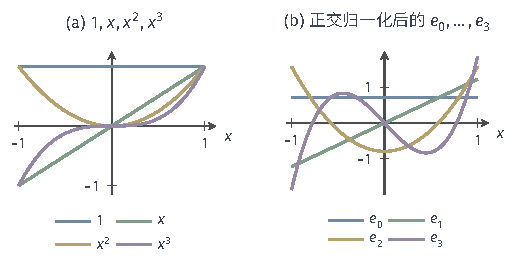
\includegraphics[width=87.3mm]{figures/02-abstract-mathematics/03-function-spaces/tikz/c1-legendre-gram-schmidt/figure.pdf}
  \caption{在$L^2[-1,1]$中对单项式做Gram--Schmidt正交化。(a)$1,x,x^2,x^3$，例如$\langle1,x^2\rangle=\tfrac23\neq0$；(b)得到的$e_0=1/\sqrt2$，$e_1=\sqrt{3/2}\,x$，$e_2=\sqrt{5/8}\,(3x^2-1)$，$e_3=\sqrt{7/8}\,(5x^3-3x)$，两两正交且范数为$1$，$e_k$在$(-1,1)$内恰有$k$个零点。}
  \label{fig:ipspace-legendre-gram-schmidt}
\end{figure}

\paragraph{完备正交系}
一个标准正交系“够不够用”，看它的有限组合能否逼近每个元素。$\{e_i\}$的有限线性组合全体记为$\operatorname{span}\{e_i\}$，它在$H$中的闭包记为$\overline{\operatorname{span}}\{e_i\}$，称为\term{闭线性张成}（closed linear span）。

\begin{definition}[完备正交系]
\label{def:ipspace-complete-orthonormal-system}
若Hilbert空间$H$中的标准正交系$\{e_i\}_{i\in I}$满足$\overline{\operatorname{span}}\{e_i\}=H$，称它为$H$的\term{完备正交系}（complete orthonormal system），也称\term{标准正交基}（orthonormal basis）或正交基。
\end{definition}

这里的“完备”与空间的完备是两个不同的概念：前者说正交系的方向够用，后者说柯西列有极限。“基”字也要小心理解。代数基要求每个元素恰是有限个基元素的组合；正交基只要求每个元素是有限组合的范数极限，允许通过极限逼近。下一节将说明，这样的极限可以写成按范数收敛的级数。

$\ell^2$中的标准单位列是完备正交系。对$x\in\ell^2$，截断$x^{(N)}=\sum_{k\leq N}x_ke_k\in\operatorname{span}\{e_k\}$满足
\[
 \lVert x-x^{(N)}\rVert^2=\sum_{k>N}\lvert x_k\rvert^2\to0,
\]
因为收敛级数的尾和趋于零。所以$\operatorname{span}\{e_k\}=c_{00}$在$\ell^2$中稠密。但$\{e_k\}$不是$\ell^2$的代数基：$(1,\tfrac12,\tfrac13,\ldots)\in\ell^2$有无穷多项非零，不是有限个$e_k$的组合。

\paragraph{完备性的正交判据}
判断一个标准正交系是否完备，常用的办法是看还有没有被它遗漏的方向。

\begin{theorem}[完备正交系的判据]
\label{thm:ipspace-completeness-criterion}
设$\{e_i\}_{i\in I}$是Hilbert空间$H$中的标准正交系。则它是完备正交系，当且仅当与每个$e_i$都正交的元素只有零。
\end{theorem}

\begin{proof}
记$M=\overline{\operatorname{span}}\{e_i\}$，它是闭线性子空间。设$M=H$，$g$与每个$e_i$正交。由内积的线性，$g$与$\operatorname{span}\{e_i\}$正交；由内积的连续性，$g$也与其闭包$M=H$正交，特别地$\langle g,g\rangle=0$，$g=0$。

反过来，设$M\neq H$，取$f\notin M$。由第~\ref{sec:ipspace-orthogonal-projection}节，$g=f-P_Mf$属于$M^\perp$，且$g\neq0$，因为$P_Mf\in M$而$f\notin M$。这个$g$与每个$e_i$正交，所以判据的条件不成立。
\end{proof}

判据的“必要”方向只用到内积的连续性，“充分”方向用到了正交投影，从而用到了完备性与闭性。例如在$L^2[-1,1]$中，偶次的归一化Legendre多项式$e_0,e_2,e_4,\ldots$组成一个无穷的标准正交系，但$x$是奇函数，与每个偶函数正交，而$x\neq0$。所以这个系不完备：方向有无穷多个，却遗漏了全部奇函数。

全体Legendre多项式$\{e_k\}_{k\geq0}$是否完备，取决于多项式能否在$L^2[-1,1]$中逼近每个元素。这需要两步逼近：连续函数在$L^2[-1,1]$中稠密，多项式又能一致逼近连续函数。这两步属于第~\ref{chap:function-approximation}章，这里不给出证明，只指出结论：Legendre多项式是$L^2[-1,1]$的完备正交系。

\paragraph{可分空间的可数正交基}
要用级数$\sum_jc_je_j$表示每个元素，正交基最好是可数的。第~\ref{chap:topological-spaces}章把具有可数稠密子集的空间称为\term{可分}（separable）空间。下面说明，对Hilbert空间而言，“有可数的正交基”与“可分”是一回事。

\begin{theorem}[可分Hilbert空间的正交基]
\label{thm:ipspace-separable-basis}
设$H$是可分Hilbert空间，$H\neq\{0\}$。则$H$有至多可数的标准正交基，并且$H$中每个标准正交系都至多可数。
\end{theorem}

\begin{proof}
取可数稠密子集$\{u_k\}_{k\geq1}$。依次检查各项，删去能由前面保留的项线性表示的项，得到一个线性无关的序列（有限或无限），其张成空间与$\operatorname{span}\{u_k\}$相同。对它做Gram--Schmidt正交化，得到标准正交系$\{e_j\}$，其张成空间仍与$\operatorname{span}\{u_k\}$相同。这个张成空间包含稠密集$\{u_k\}$，所以在$H$中稠密，$\{e_j\}$是至多可数的完备正交系。

再设$\{e_i\}_{i\in I}$是任意标准正交系。对$i\neq j$，$\lVert e_i-e_j\rVert^2=\lVert e_i\rVert^2+\lVert e_j\rVert^2=2$。所以以各$e_i$为中心、半径$\tfrac{\sqrt2}2$的开球两两不交。每个开球都含有稠密集$\{u_k\}$中的点，不同的球含有不同的点，于是$i\mapsto$（球中某个$u_k$的下标$k$）是$I$到$\mathbb N_+$的单射，$I$至多可数。
\end{proof}

反方向也成立：若$H$有可数的正交基$\{e_j\}$，则系数取有理数（复情形取实部、虚部为有理数）的有限组合构成可数集，并且在$H$中稠密，所以$H$可分。$\ell^2$有可数的正交基$\{e_k\}$，因而可分；由上面所述的Legendre多项式的完备性，$L^2[-1,1]$也可分。不可分的Hilbert空间也存在，那时正交基不可数，下一节的级数需要改写为不可数族的求和，本书不展开。

\section{正交展开}
\label{sec:ipspace-orthogonal-expansions}

有了可数的标准正交系，就可以写出级数$\sum_jc_je_j$。第~\ref{chap:functions-as-vectors}章指出，级数要回答三个问题：是否收敛、表示哪些元素、系数是否唯一。本节在Hilbert空间中用范数收敛回答它们：系数由内积给出，有限截断是正交投影，完备正交系给出收敛的展开与能量恒等式，不完备的正交系只恢复它张成的那一部分。

本节设$H$是Hilbert空间，$\{e_j\}$是有限或可数的标准正交系，下标按$j=1,2,\ldots$排列。对$f\in H$，称
\[
 c_j=\langle e_j,f\rangle
\]
为$f$关于$\{e_j\}$的系数。

\paragraph{有限截断是正交投影}
先看只保留有限个方向时的情形。记$M_n=\operatorname{span}\{e_1,\ldots,e_n\}$，它是有限维子空间，因而闭，第~\ref{sec:ipspace-orthogonal-projection}节的结论适用。

\begin{theorem}[有限截断]
\label{thm:ipspace-finite-truncation}
对$f\in H$与$n\geq1$，令$s_n=\sum_{j=1}^nc_je_j$。则$s_n=P_{M_n}f$，并且
\begin{equation}
 \lVert f-s_n\rVert^2=\lVert f\rVert^2-\sum_{j=1}^n\lvert c_j\rvert^2 .
 \label{eq:ipspace-truncation-error}
\end{equation}
\end{theorem}

\begin{proof}
$s_n\in M_n$。对每个$k\leq n$，由标准正交性$\langle e_k,s_n\rangle=\sum_jc_j\langle e_k,e_j\rangle=c_k$，所以$\langle e_k,f-s_n\rangle=c_k-c_k=0$。$f-s_n$与$M_n$的每个基元素正交，因而与$M_n$正交；由正交刻画，$s_n=P_{M_n}f$。再由勾股关系$\lVert f\rVert^2=\lVert s_n\rVert^2+\lVert f-s_n\rVert^2$与$\lVert s_n\rVert^2=\sum_{j\leq n}\lvert c_j\rvert^2$即得式~\eqref{eq:ipspace-truncation-error}。
\end{proof}

这个定理说明，用内积计算的系数就是$M_n$中的最佳选择：在$e_1,\ldots,e_n$的所有组合中，$s_n$离$f$最近。增加一个方向时，已经算好的系数不需要修改，误差平方恰好减少新系数的模平方。若$\{e_j\}$只是线性无关而不正交，这两件事都不成立，系数要重新解一个Gram矩阵方程组。

\paragraph{Bessel不等式}
式~\eqref{eq:ipspace-truncation-error}的左边非负，所以对每个$n$都有$\sum_{j\leq n}\lvert c_j\rvert^2\leq\lVert f\rVert^2$。令$n\to\infty$，得到下面的不等式。

\begin{theorem}[Bessel不等式]
\label{thm:ipspace-bessel}
对$f\in H$，$\sum_j\lvert\langle e_j,f\rangle\rvert^2\leq\lVert f\rVert^2$。
\end{theorem}

非负项级数的部分和有界，所以级数收敛，和不超过这个界。特别地$c_j\to0$：任何元素在越来越靠后的正交方向上的分量都越来越小。这一结论只用到正交系，不要求它完备，也不要求$H$完备。

\paragraph{级数的收敛与和}
Bessel不等式说明系数平方可和。反过来，平方可和的系数总能给出一个收敛的级数，它的和就是$f$在闭张成空间上的投影。

\begin{theorem}[正交展开]
\label{thm:ipspace-orthogonal-expansion}
设$M=\overline{\operatorname{span}}\{e_j\}$。
\begin{enumerate}
 \item 对数列$(a_j)$，级数$\sum_ja_je_j$依范数收敛，当且仅当$\sum_j\lvert a_j\rvert^2<\infty$；此时$\lVert\sum_ja_je_j\rVert^2=\sum_j\lvert a_j\rvert^2$。
 \item 对$f\in H$，级数$\sum_jc_je_j$依范数收敛，其和为$P_Mf$。
\end{enumerate}
\end{theorem}

\begin{proof}
（1）记部分和$t_n=\sum_{j\leq n}a_je_j$。对$n>m$，由标准正交性，$\lVert t_n-t_m\rVert^2=\sum_{m<j\leq n}\lvert a_j\rvert^2$。所以$(t_n)$是柯西列当且仅当$\sum_j\lvert a_j\rvert^2$的部分和是柯西数列，即级数收敛。$H$完备，柯西列收敛；反之收敛列是柯西列。范数等式由$\lVert t_n\rVert^2=\sum_{j\leq n}\lvert a_j\rvert^2$与范数的连续性得到。

（2）由Bessel不等式和（1），$s_n=\sum_{j\leq n}c_je_j$收敛到某个$s$。每个$s_n\in M$，$M$闭，所以$s\in M$。对固定的$k$与$n\geq k$，$\langle e_k,f-s_n\rangle=0$；令$n\to\infty$，由内积的连续性得$\langle e_k,f-s\rangle=0$。于是$f-s$与$\operatorname{span}\{e_j\}$正交，再由连续性与其闭包$M$正交。由正交刻画，$s=P_Mf$。
\end{proof}

（1）中的“仅当”方向不需要完备性，“当”方向需要：在不完备的$c_{00}$中，$\sum_ka_ke_k$对$a_k=1/k$就不收敛。（2）也回答了唯一性：若$\sum_ja_je_j=g$依范数收敛，与$e_k$作内积并取极限，得$a_k=\langle e_k,g\rangle$，系数只能是内积系数。由于（2）对$\{e_j\}$的任何排列都成立，和总是$P_Mf$，所以级数的和不依赖求和次序。

\paragraph{完备正交系：展开与Parseval等式}
若$\{e_j\}$是完备正交系，则$M=H$，$P_Mf=f$，得到最重要的情形。

\begin{theorem}[Parseval等式]
\label{thm:ipspace-parseval}
设$\{e_j\}$是$H$的完备正交系，$f,g\in H$，$c_j=\langle e_j,f\rangle$，$d_j=\langle e_j,g\rangle$。则
\[
 f=\sum_jc_je_j\quad(\text{依范数}),\qquad \lVert f\rVert^2=\sum_j\lvert c_j\rvert^2,\qquad \langle f,g\rangle=\sum_j\overline{c_j}\,d_j .
\]
\end{theorem}

\begin{proof}
展开式由定理~\ref{thm:ipspace-orthogonal-expansion}（2）与$M=H$得到。在式~\eqref{eq:ipspace-truncation-error}中令$n\to\infty$，左边趋于零，得范数等式，称为\term{Parseval等式}（Parseval identity）。对内积，$\langle s_n,t_n\rangle=\sum_{j\leq n}\overline{c_j}d_j$，其中$t_n$是$g$的部分和；由内积的连续性，左边趋于$\langle f,g\rangle$。
\end{proof}

Parseval等式说明，当正交基为可数无穷时，取系数$f\mapsto(c_j)$把$H$一一地映成$\ell^2$，并保持内积：每个$f$给出平方可和的系数，每个平方可和的系数列由定理~\ref{thm:ipspace-orthogonal-expansion}（1）给出唯一的元素。所以一个具有可数正交基的无限维Hilbert空间，在选定正交基后，与$\ell^2$只有记号的差别，就像有限维内积空间选定标准正交基后与$\mathbb K^d$只有记号的差别一样。

由式~\eqref{eq:ipspace-truncation-error}与Parseval等式，截断误差可以直接从系数读出：
\begin{equation}
 \lVert f-s_n\rVert^2=\sum_{j>n}\lvert c_j\rvert^2 ,
 \label{eq:ipspace-tail-error}
\end{equation}
即系数平方的尾和。误差随$n$单调下降并趋于零，下降的快慢完全由系数衰减的快慢决定。

\paragraph{不完备时只恢复闭张成中的部分}
若$\{e_j\}$不完备，展开的和是$P_Mf$而不是$f$，正交补$M^\perp$中的分量永远丢失。Bessel不等式与Parseval等式之间的差$\lVert f\rVert^2-\sum_j\lvert c_j\rvert^2=\lVert f-P_Mf\rVert^2$，正是丢失部分的能量。

回到偶次Legendre多项式。设$E$为$L^2[-1,1]$中几乎处处满足$f(-x)=f(x)$的元素组成的子空间。任意$f$都可以写成$f(x)=\tfrac{f(x)+f(-x)}2+\tfrac{f(x)-f(-x)}2$，前者是偶函数，属于$E$，后者是奇函数，与$E$正交。由正交分解的唯一性，$P_Ef(x)=\tfrac{f(x)+f(-x)}2$，并且$E$就是这个投影的像。偶次Legendre多项式是偶函数，它们的闭张成含于$E$。反过来，对$f\in E$，奇次的$e_k$是奇函数，$\langle e_k,f\rangle=0$；由上一节所述的全体Legendre多项式的完备性，$f$的展开只含偶次项，所以$f$属于偶次Legendre多项式的闭张成。于是这个闭张成恰为$E$，只用偶次方向展开时，和就是$P_Ef$。

取$f=e^x$，得$P_Ef=\cosh x$，丢失的部分是奇部$\sinh x$，见图~\ref{fig:ipspace-even-odd-projection}。距离平方为
\[
 \int_{-1}^1\sinh^2x\,dx=\frac{\sinh2}{2}-1\approx0.813 ,
\]
无论加入多少偶次方向都无法减小。

\begin{figure}[!htb]
  \centering
  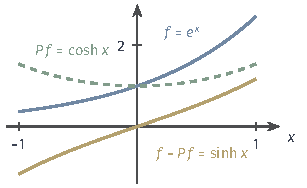
\includegraphics[width=51.9mm]{figures/02-abstract-mathematics/03-function-spaces/tikz/c1-even-odd-projection/figure.pdf}
  \caption{向偶函数子空间的正交投影。$[-1,1]$上$f(x)=e^x$，投影$P_Ef=\cosh x$为其偶部，误差$f-P_Ef=\sinh x$为奇函数，与每个偶函数正交。只用偶次方向展开$e^x$时，误差始终至少为$\lVert\sinh\rVert_2\approx0.90$。}
  \label{fig:ipspace-even-odd-projection}
\end{figure}

\paragraph{截断误差的例子}
用全体Legendre多项式展开符号函数$\operatorname{sgn}$。它是奇函数，只有奇次系数非零，$\lVert\operatorname{sgn}\rVert_2^2=2$。由$e_1=\sqrt{3/2}\,x$，$c_1=\sqrt{3/2}\int_{-1}^1\lvert x\rvert\,dx=\sqrt{3/2}$，$c_1^2=\tfrac32$。由$e_3=\sqrt{7/8}\,(5x^3-3x)$，$\int_{-1}^1\operatorname{sgn}(x)(5x^3-3x)\,dx=2(\tfrac54-\tfrac32)=-\tfrac12$，所以$c_3^2=\tfrac78\cdot\tfrac14=\tfrac7{32}$。同样可算$c_5^2=\tfrac{11}{128}$。由式~\eqref{eq:ipspace-tail-error}，截断误差
\[
 \lVert\operatorname{sgn}-s_1\rVert_2^2=2-\frac32=0.5,\qquad \lVert\operatorname{sgn}-s_5\rVert_2^2=2-\frac32-\frac7{32}-\frac{11}{128}\approx0.195 .
\]

图~\ref{fig:ipspace-legendre-truncation}(a)画出了部分和，(b)把$\operatorname{sgn}$与$\lvert x\rvert$的截断误差放在一起。精确计算给出：$\operatorname{sgn}$在$n=15$时误差约为$0.077$，$n=41$时仍约为$0.030$；$\lvert x\rvert$连续，只在$0$处有折角，$n=2$时误差已约为$0.0104$，$n=40$时约为$6\times10^{-6}$。两者都趋于零，但速度相差很大。这里只是两个例子的观察；系数衰减与函数光滑性之间的一般关系属于第~\ref{chap:function-approximation}章。

\begin{figure}[!htb]
  \centering
  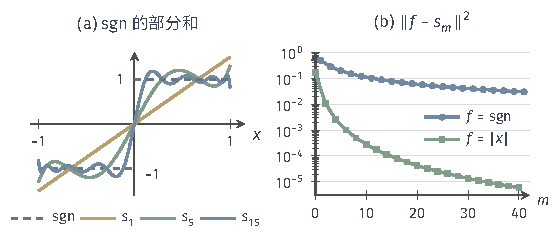
\includegraphics[width=94.9mm]{figures/02-abstract-mathematics/03-function-spaces/tikz/c1-legendre-truncation/figure.pdf}
  \caption{Legendre展开的截断。(a)$\operatorname{sgn}$（虚线）与部分和$s_1,s_5,s_{15}$，其中$s_1=\tfrac32x$；部分和是多项式，在跳跃点附近来回振荡。(b)截断误差$\lVert f-s_n\rVert_2^2$（对数纵轴）：$\operatorname{sgn}$取奇数$n$，$\lvert x\rvert$取偶数$n$。两条曲线都单调趋于零，有跳跃的$\operatorname{sgn}$下降慢得多。}
  \label{fig:ipspace-legendre-truncation}
\end{figure}

\paragraph{范数收敛不是点态收敛}
式~\eqref{eq:ipspace-tail-error}只控制$L^2$误差，不控制任何一点处的值。图~\ref{fig:ipspace-legendre-truncation}(a)中的部分和都是连续函数；若它们一致收敛，极限必然连续，而$\operatorname{sgn}$在$0$处跳跃，没有连续代表，所以部分和不一致收敛到$\operatorname{sgn}$，尽管$L^2$误差趋于零。在$x=0$处，每个部分和都是奇多项式，取值为$0$；而$\operatorname{sgn}$作为$L^2$元素在$0$处根本没有确定的值，谈不上收敛到什么。

更一般地，$L^2$中的元素是等价类，“展开在点$x_0$处收敛到$f(x_0)$”首先要求$f(x_0)$有意义，其次需要“点值受范数控制”这样的额外条件。由第~\ref{chap:normed-spaces}章，$L^2$收敛的序列有几乎处处收敛的子列，但整列部分和是否逐点收敛，要看具体的正交系与函数的正则性。点值读取何时连续，是第~\ref{chap:linear-functionals}章和第~\ref{chap:rkhs}章的问题；三角级数的逐点与一致收敛条件，在第~\ref{chap:fourier-transform}章讨论。

\section{本章小结}
\label{sec:ipspace-summary}

章首的两个问题都靠内积回答。内积的公理与维数无关，复情形约定对第二个变量线性、对第一个变量共轭线性；Cauchy--Schwarz不等式使$\sqrt{\langle f,f\rangle}$成为范数，并使内积连续。内积范数满足平行四边形恒等式，一致范数与$L^1$范数不满足，所以它们不来自任何内积。

Hilbert空间是在诱导范数下完备的内积空间，也就是范数来自内积的Banach空间。有限维时完备性自动成立，无限维时不然：有限支撑数列和平方积分下的连续函数都是不完备的内积空间。$L^2(\mu)$把平方可积函数的等价类收进来，乘积积分在Hölder不等式下有定义，诱导的正是$L^2$范数，由第~\ref{chap:normed-spaces}章的完备性直接成为Hilbert空间；计数测度下得到$\ell^2$。

在Hilbert空间的闭子空间上，最佳逼近存在且唯一：平行四边形恒等式使极小化序列成为柯西列，完备性给出极限，闭性保证极限留在子空间中。最近点由误差与子空间正交刻画，定义为正交投影，给出唯一的正交分解与勾股关系；有限支撑数列在$\ell^2$中的例子说明闭性不能去掉。一般闭凸集上最近点仍存在唯一，但正交条件要换成变分不等式，归卷五处理。

完备正交系只要求有限组合在范数下稠密，与只允许有限组合的代数基不同；它可以用“与所有方向正交的只有零”来检验，可分Hilbert空间的正交基至多可数，并可由Gram--Schmidt正交化得到。用内积系数展开时，有限截断就是正交投影，Bessel不等式控制系数；完备正交系给出依范数收敛的展开、Parseval等式和尾和形式的截断误差，并使空间与$\ell^2$同构；不完备时只恢复闭张成中的部分。范数收敛不等于点态收敛，Legendre部分和在$L^2$中收敛到$\operatorname{sgn}$，却不一致收敛。

这些结构为后面的章节准备了依据。第~\ref{chap:linear-functionals}章用正交投影证明连续线性泛函都能表示为内积，从而用内积表示观测；第~\ref{chap:fourier-transform}章和第~\ref{chap:wavelet-transform}章分别证明三角函数系与小波系的完备性；截断误差的衰减速度与函数光滑性的关系，由第~\ref{chap:function-approximation}章研究。


\chapter{函数类的有限覆盖}
\label{chap:function-class-covers}

设想要预先造好一张函数表，以后无论遇到某一类中的哪个函数，都能从表里查到一行，使它与该函数的最大误差不超过$0.1$。表必须在看到具体函数之前造好，而且只能有有限行。这样的表是否存在，至少需要多少行？

第~\ref{chap:functions-as-vectors}章把函数看作无限维向量，下标是输入$x$，分量是取值$f(x)$。沿着这个类比，一张函数表就是有限个向量，查表就是找最近的向量。在有限维里答案现成：把$\mathbb R^n$中的立方体切成小方块，每个坐标只有有限种取值，方块数是每坐标取值数的$n$次方。可是坐标数趋于无穷时，这个数也趋于无穷。

所以本章的问题可以这样问：一类函数要受到怎样的共同限制，无穷多个坐标才能压缩成有限个有效坐标？答案有两条路线。第一条看取值列，要求相邻坐标互相牵制，只记录有限个位置；第二条看系数列，要求靠后的坐标足够小，只保留前面有限项。

第~\ref{sec:fcover-problem}节把函数表写成覆盖数，并说明只限制范数不够。第~\ref{sec:fcover-arzela-ascoli}节用一致有界与等度连续回答能否覆盖。第~\ref{sec:fcover-construction}节把第一条路线做成可以计数的构造，第~\ref{sec:fcover-finite-representations}节给出第二条路线。这里只研究确定性的计数，怎样构造满足统一逼近前提的有限表示留给第~\ref{chap:function-approximation}章。

\section{有限覆盖问题}
\label{sec:fcover-problem}

函数表问题有三个要素：一类函数，一个衡量误差的距离，一个精度。本节先把它们写成覆盖数，再用有限维的立方体作参照，比较为单个函数找近似与为整类函数造表这两种要求，最后说明只限制范数为什么不够。

\paragraph{函数类与覆盖数}

我们把要讨论的一组函数称为\term{函数类}（function class），记为$\mathcal F$。它总放在某个由函数组成的度量空间$(E,\rho)$中，距离$\rho$就是衡量误差的标准。本章用到的两种距离是
\[
 \lVert f-g\rVert_\infty=\sup_{x\in K}\lvert f(x)-g(x)\rvert,\qquad
 \lVert f-g\rVert_1=\int_0^1\lvert f-g\rvert\,dx .
\]
前者用在紧集$K$上的连续函数空间$C(K)$中，后者用在$L^1[0,1]$中。

函数表的一行就是$E$中的一个函数。表能服务于整类，意思是$\mathcal F$的每个成员都落在某一行的半径$\varepsilon$闭球内。第~\ref{chap:metric-spaces}章把所需的最少行数定义为覆盖数：
\begin{equation}
 N_E(\varepsilon,\mathcal F)=\min\Bigl\{N:\ \exists\,g_1,\ldots,g_N\in E,\
 \mathcal F\subseteq\bigcup_{j=1}^NB[g_j,\varepsilon]\Bigr\},
 \label{eq:fcover-covering-number}
\end{equation}
没有有限覆盖时记为$+\infty$。

覆盖数的对数$\log N_E(\varepsilon,\mathcal F)$称为度量熵。它的含义很具体：给表中的行编号需要$\lceil\log_2N\rceil$个二进制位，例如$N=1024$时需要$10$位。发送这几位，对方查表就能以误差$\varepsilon$复原类中的成员。所以度量熵是在精度$\varepsilon$下识别一个成员所需的信息量。

表中的行可以有两种约定。$N_E(\varepsilon,\mathcal F)$允许行取$E$中任意函数，例如后面用插值造出的折线，它们未必属于$\mathcal F$。$N_{\mathcal F}(\varepsilon,\mathcal F)$要求每一行本身就是类中成员。第~\ref{chap:metric-spaces}章证明了两者只差把精度减半：
\begin{equation}
 N_E(\varepsilon,\mathcal F)\leq N_{\mathcal F}(\varepsilon,\mathcal F)\leq N_E(\varepsilon/2,\mathcal F).
 \label{eq:fcover-center-change}
\end{equation}

右边的不等式后面要反复使用，这里重述它的机制。取一个中心在$E$中的$\varepsilon/2$覆盖，删去与$\mathcal F$不相交的球，在每个余下的球中任选一个成员$g$代替原中心$c$。原来落在该球中的成员$f$到$g$的距离满足
\[
 \rho(f,g)\leq\rho(f,c)+\rho(c,g)\leq\frac\varepsilon2+\frac\varepsilon2=\varepsilon .
\]
所以更换中心不增加行数，只把半径放大一倍。

\paragraph{从立方体到函数}

先看有限维。在$\mathbb R^n$中取最大分量距离
\[
 \lVert a-b\rVert_\infty=\max_k\lvert a_k-b_k\rvert ,
\]
它是一致距离在有限个下标上的版本。半径$\varepsilon$的闭球是边长$2\varepsilon$的小立方体，条件$\lVert a-b\rVert_\infty\leq\varepsilon$就是每个坐标都在$b_k$的$\varepsilon$范围内。

要覆盖立方体$[-M,M]^n$，只需每个坐标各选一组刻度。令$T=\lceil M/\varepsilon\rceil$，取刻度
\[
 c_k=-M+(2k-1)\varepsilon,\qquad k=1,\ldots,T .
\]
区间$[c_k-\varepsilon,c_k+\varepsilon]$首尾相接，覆盖了$[-M,M]$，所以每个坐标都能选到距离不超过$\varepsilon$的刻度。

各坐标的刻度可以任意搭配，全部搭配共$T^n$种，于是
\begin{equation}
 N_{\mathbb R^n}\bigl(\varepsilon,[-M,M]^n\bigr)\leq\Bigl\lceil\frac M\varepsilon\Bigr\rceil^n,\qquad
 \log N_{\mathbb R^n}\leq n\log\Bigl\lceil\frac M\varepsilon\Bigr\rceil .
 \label{eq:fcover-cube}
\end{equation}
度量熵的结构是“坐标个数乘以每个坐标的信息量”，本章后面的上界都是这个结构。

用一个小例子走一遍。下面取$n=3$、$M=1$、$\varepsilon=1/4$，于是$T=4$，刻度为
\[
 -\frac34,\quad -\frac14,\quad \frac14,\quad \frac34 .
\]
式~\eqref{eq:fcover-cube}给出至多$4^3=64$个中心。向量$(0.3,-0.6,0.9)$的最近搭配是$(1/4,-3/4,3/4)$，三个坐标的误差依次是$0.05$、$0.15$、$0.15$，都不超过$1/4$。

函数的情形完全类比。在一致距离下，以$g$为中心、半径$\varepsilon$的闭球由满足
\[
 g(x)-\varepsilon\leq f(x)\leq g(x)+\varepsilon\qquad\text{对所有}\ x
\]
的函数$f$组成。这是图像周围的一条管道，正是小立方体在无穷多个坐标上的样子。

\begin{BookInlineFigure}
  \centering
  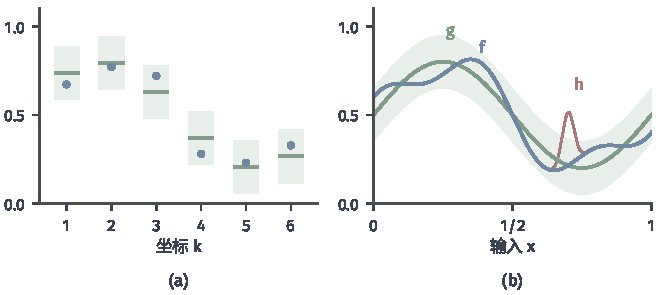
\includegraphics[width=112mm]{figures/04-spaces-measures-and-geometry/03-function-spaces/matplotlib/fcover-cube-tube/figure.pdf}
  \caption{一致距离的闭球。(a)绿色短线是代表$g$的六个坐标，绿色方框是各坐标$\pm\varepsilon$的范围（$\varepsilon=0.15$）；蓝点$f$的六个坐标都在方框内，表示$f$在这个闭球里。(b)同样的$g$与$f$画在全部输入上，方框连成管道。红色的$h$只在一小段上越出管道，一致距离仍把它判在球外。}
  \label{fig:fcover-cube-tube}
\end{BookInlineFigure}

图~\ref{fig:fcover-cube-tube}中，$f$在(a)的每个坐标上都落入方框，(b)中整条曲线留在管道里。一致距离只看最坏的坐标，$h$在别处都贴近$g$，在一小段上越出管道就算不合格。

类比也在这里显出困难。式~\eqref{eq:fcover-cube}的右端随$n$增大而趋于无穷，函数有无穷多个坐标，不能直接套用。真正的问题是：一类函数的无穷多个坐标，能否只用有限多个就决定到精度$\varepsilon$？

\paragraph{挑选近似与统一精度}

先看为单个函数找近似。给定$f\in C[0,1]$和$\varepsilon>0$，$f$在紧区间上一致连续，存在$m$，使$\lvert x-y\rvert\leq1/m$时$\lvert f(x)-f(y)\rvert\leq\varepsilon$。连接点$(j/m,f(j/m))$（$j=0,\ldots,m$）得到折线$g$。

设$x$在第$j$段上，局部位置为$t\in[0,1]$，则$g(x)$是两端值的凸组合，
\[
 f(x)-g(x)=(1-t)\Bigl(f(x)-f\bigl(\tfrac jm\bigr)\Bigr)+t\Bigl(f(x)-f\bigl(\tfrac{j+1}m\bigr)\Bigr).
\]
括号内的两项绝对值都不超过$\varepsilon$，所以$\lvert f(x)-g(x)\rvert\leq\varepsilon$。

这说明每个连续函数都有由$m+1$个数决定的近似，但$m$取决于$f$变化的快慢。为整类函数造表，要求的量词次序不同。两种说法分别是
\[
 \begin{gathered}
 \forall f\in\mathcal F,\ \exists\text{有限描述}\ g_f:\ \rho(f,g_f)\leq\varepsilon,\\
 \exists\text{有限集}\ V\subseteq E,\ \forall f\in\mathcal F,\ \exists v\in V:\ \rho(f,v)\leq\varepsilon .
 \end{gathered}
\]

第一种说法对$C[0,1]$总成立，第二种则要求一份预算服务全类。有限类总能造表，把成员全部列出即可。困难出在无限类上：若所需的节点数$m$随成员无限增大，就没有共同的预算，后面的鼓包正是这样。

\paragraph{距离的选择}

同一类函数在不同距离下可以有不同的答案。向量的情形已经能看出原因：两个$n$维向量只在一个坐标上相差$1$，最大分量差是$1$，平均分量差却只有$1/n$。

取$[0,1]$上的指示函数族$\mathcal F=\{\mathbf 1_{[0,t]}:0\leq t\leq1\}$，每个成员在某一点跳变。在$L^1[0,1]$中，两个成员之差的积分就是图~\ref{fig:fcover-indicator-distances}(b)中矩形的面积：
\[
 \lVert\mathbf 1_{[0,t]}-\mathbf 1_{[0,s]}\rVert_1=\lvert t-s\rvert .
\]
于是覆盖$\mathcal F$等同于用长度$2\varepsilon$的闭区间覆盖参数区间$[0,1]$。

\begin{BookInlineFigure}
  \centering
  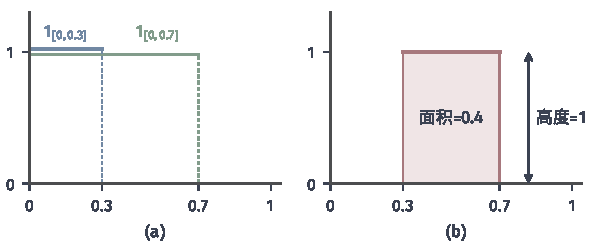
\includegraphics[width=100mm]{figures/04-spaces-measures-and-geometry/03-function-spaces/matplotlib/fcover-indicator-distances/figure.pdf}
  \caption{同一对函数的两种距离。(a)$\mathbf 1_{[0,0.3]}$（蓝）与$\mathbf 1_{[0,0.7]}$（绿）。(b)差的绝对值：$L^1$距离是红色矩形的面积$0.4$，一致距离是矩形的高度$1$。跳变点越靠近，面积越小，高度却始终是$1$。}
  \label{fig:fcover-indicator-distances}
\end{BookInlineFigure}

取$N=\lceil1/(2\varepsilon)\rceil$及$t_j=(2j-1)/(2N)$，每个$t$到最近的$t_j$不超过$1/(2N)\leq\varepsilon$，所以
\[
 N_{\mathcal F}(\varepsilon,\mathcal F)\leq\Bigl\lceil\frac1{2\varepsilon}\Bigr\rceil .
\]
例如$\varepsilon=0.1$时$N=5$，五个中心的跳变点是$0.1,0.3,0.5,0.7,0.9$。成员$\mathbf 1_{[0,0.62]}$对应最近的中心$t=0.7$，误差为$0.08$。

把同一族函数看作$[0,1]$上的有界函数，改用一致距离，情形就变了。$t\neq s$时两个指示函数在$t$与$s$之间相差$1$，所以两两距离都是$1$。半径$\varepsilon<1/2$的闭球若含其中两个，两者距离至多$2\varepsilon<1$，矛盾，因此每个球至多含一个成员。成员有不可数多个，覆盖数为$+\infty$。

积分距离允许误差集中在测度很小的集合上，一致距离不允许，两种答案的分界就在这里。

\paragraph{范数界不能保证有限覆盖}

最直接的约束是给出范数上界，即把$\mathcal F$放进一个闭球。这相当于把每个坐标限制在$[-M,M]$中，在有限维已足够，在无限维却不够。第~\ref{chap:functions-as-vectors}章用Riesz引理证明：任何无限维赋范空间的闭单位球中都有一列单位向量，两两距离至少为$1/2$。

半径$r<1/4$的闭球若含其中两个，两者距离至多$2r<1/2$，矛盾。所以无限维空间的闭单位球不能被半径小于$1/4$的有限个闭球覆盖。按比例缩放，半径$R$的闭球不能被半径小于$R/4$的有限个闭球覆盖。

在$C[0,1]$中可以把这一现象看得很具体。第~\ref{chap:functions-as-vectors}章的鼓包$\varphi_n$在$[\tfrac1{n+1},\tfrac1n]$的中点取$1$，在两端取$0$，区间外恒为$0$。不同鼓包的支撑至多相接于一点，所以$n\neq l$时
\[
 \lVert\varphi_n-\varphi_l\rVert_\infty=1 .
\]
全部$\varphi_n$都在闭单位球内，却没有半径小于$1/2$的有限覆盖。

\begin{BookInlineFigure}
  \centering
  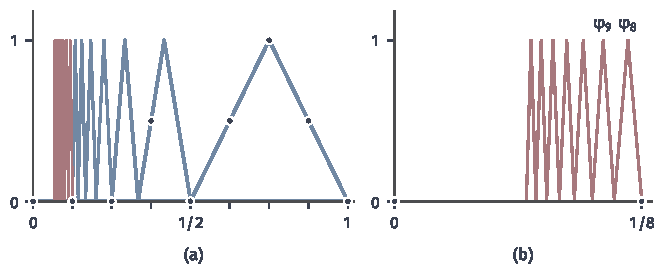
\includegraphics[width=112mm]{figures/04-spaces-measures-and-geometry/03-function-spaces/matplotlib/fcover-tents-on-grid/figure.pdf}
  \caption{固定网格看不见足够窄的鼓包。黑点是节点$j/8$。(a)蓝色为$\varphi_1,\ldots,\varphi_7$，红色为$\varphi_8,\ldots,\varphi_{14}$。(b)把$[0,1/8]$放大：红色鼓包的支撑全在两个节点之间，节点上的值都是$0$。}
  \label{fig:fcover-tents-on-grid}
\end{BookInlineFigure}

失败的原因可以从图~\ref{fig:fcover-tents-on-grid}读出来。固定一组节点$j/m$，当$n\geq m$时，$\varphi_n$的支撑含于$[0,1/m]$，内部没有节点，于是$\varphi_n$在每个节点上都为$0$。这些鼓包与零函数记录相同，一致距离却是$1$。

这也解释了斜率的作用。$\varphi_n$从$0$升到$1$只用了长度$1/(2n(n+1))$的区间，斜率为$2n(n+1)$，随$n$无界。用向量的语言说，每个鼓包占据一段自己的“坐标”，互相之间没有牵制，就像标准单位向量$e_n$。

要补上缺失的条件，有两个方向。第~\ref{sec:fcover-arzela-ascoli}节要求全类共用一个连续性尺度，让相邻坐标互相牵制；第~\ref{sec:fcover-finite-representations}节要求全类都贴近同一个有限维子空间，让靠后的坐标足够小。

\section{Arzelà--Ascoli判据}
\label{sec:fcover-arzela-ascoli}

上一节的帽形函数说明，函数类缺少共同的连续性尺度时，有限个位置上的值无法代表整个函数。本节把这一观察变成判据：在紧度量空间$K$上，连续函数类在一致距离下全有界，当且仅当它一致有界并且等度连续。全节中$C(K)$表示$K$上实值或复值连续函数的全体，距离取$\lVert f-g\rVert_\infty$；两种取值情形的论证相同，只在量化取值时分别处理实轴上的区间与复平面上的正方形。

\paragraph{一致有界与等度连续}

覆盖要求有限个代表照顾到每个成员，因此类中函数至少要共同受到两方面的约束：取值不能任意大，变化不能任意快。第一个约束是幅度上的。

\begin{definition}[一致有界]
\label{def:fcover-uniformly-bounded}
设$K$是集合，$\mathcal F$是$K$上一族实值或复值函数。若存在常数$M$，使$\lvert f(x)\rvert\leq M$对所有$f\in\mathcal F$和所有$x\in K$成立，就称$\mathcal F$\term{一致有界}（uniformly bounded）。
\end{definition}

对$\mathcal F\subseteq C(K)$，一致有界就是$\sup_{f\in\mathcal F}\lVert f\rVert_\infty<\infty$，即$\mathcal F$含于一个一致范数球中。上一节的帽形函数说明，仅有这一条还不够。

第二个约束是变化上的，它就是第~\ref{chap:metric-space-maps}章的等度连续性：对每个$x\in K$和$\varepsilon>0$，有一个对全族都有效的半径$\delta$，使$d(x,y)<\delta$时$\lvert f(x)-f(y)\rvert<\varepsilon$对所有$f\in\mathcal F$成立。那里还证明了，定义域紧时这个半径可以进一步取得与$x$无关。下面使用的正是这一统一形式：对每个$\varepsilon>0$，存在$\delta>0$，使
\begin{equation}
d(x,y)<\delta\ \Longrightarrow\ \lvert f(x)-f(y)\rvert<\varepsilon\qquad\text{对所有}\ f\in\mathcal F\ \text{及}\ x,y\in K.
\label{eq:fcover-uniform-equicontinuity}
\end{equation}

最常见的等度连续族共用一个Lipschitz常数。若每个$f\in\mathcal F$都满足$\lvert f(x)-f(y)\rvert\leq L\,d(x,y)$，取$\delta=\varepsilon/L$即可满足式\eqref{eq:fcover-uniform-equicontinuity}。反过来，上一节的帽形函数$\varphi_k$不等度连续：对任意$\delta>0$，取$k$使$r_k<\delta$，点$x=c_k$与$y=c_k+r_k$相距$r_k<\delta$，却有$\lvert\varphi_k(x)-\varphi_k(y)\rvert=1$。$[0,1]$上的$x^n$也是这样，第~\ref{chap:functions-as-vectors}章已看到它们一致有界却没有一致收敛的子列。

\paragraph{判据与证明}

两个约束合起来恰好刻画全有界性。在陈述之前回忆两件事：$C(K)$在一致距离下完备（第~\ref{chap:normed-spaces}章）；在完备度量空间中，子集相对紧（闭包紧）当且仅当它全有界（第~\ref{chap:metric-spaces}章）。

\begin{theorem}[Arzelà--Ascoli判据]
\label{thm:fcover-arzela-ascoli}
设$(K,d)$是非空紧度量空间，$\mathcal F\subseteq C(K)$，距离取一致距离。则下列三条等价：
\begin{enumerate}
\item $\mathcal F$一致有界且等度连续；
\item $\mathcal F$全有界，即对每个$\varepsilon>0$都有$N_{\mathcal F}(\varepsilon,\mathcal F)<\infty$；
\item $\mathcal F$在$C(K)$中相对紧。
\end{enumerate}
进一步，$\mathcal F$在$C(K)$中紧，当且仅当它满足上述条件并且是$C(K)$的闭子集。
\end{theorem}

证明的核心是有限化：等度连续允许只在有限个位置上观察函数，一致有界允许把这些位置上的值归入有限个小块，于是整类函数只留下有限种“记录”。

\begin{proof}
由1推出2。设$\lvert f\rvert\leq M$对所有$f\in\mathcal F$成立，给定$\varepsilon>0$。由式\eqref{eq:fcover-uniform-equicontinuity}取$\delta>0$，使$d(x,y)<\delta$时$\lvert f(x)-f(y)\rvert<\varepsilon/4$对所有$f$成立。紧空间全有界，所以有有限个点$x_1,\ldots,x_p\in K$，使每个$x\in K$都满足某个$d(x,x_i)<\delta$。

再把取值集合$\{z:\lvert z\rvert\leq M\}$分成有限个直径不超过$\varepsilon/4$的小块：实值时用长度不超过$\varepsilon/4$的小区间，复值时用边长不超过$\varepsilon/(4\sqrt2)$的小正方形，并约定各块互不相交。对每个$f\in\mathcal F$，记下$f(x_1),\ldots,f(x_p)$分别落在哪一块，这一串块编号称为$f$的记录。块数有限、位置数有限，所以记录只有有限种。

对每一种实际出现的记录，从$\mathcal F$中任取一个具有该记录的成员作为代表。若$f$与代表$g$记录相同，则$\lvert f(x_i)-g(x_i)\rvert\leq\varepsilon/4$对每个$i$成立。对任意$x\in K$，取$x_i$使$d(x,x_i)<\delta$，由三角不等式，
\[
\lvert f(x)-g(x)\rvert\leq\lvert f(x)-f(x_i)\rvert+\lvert f(x_i)-g(x_i)\rvert+\lvert g(x_i)-g(x)\rvert<\frac{3\varepsilon}{4}.
\]
所以有限个代表构成中心在$\mathcal F$中的$\varepsilon$覆盖，$N_{\mathcal F}(\varepsilon,\mathcal F)<\infty$。

由2推出1。取一个有限的$1$覆盖$f_1,\ldots,f_N\in\mathcal F$，每个$f$都满足某个$\lVert f-f_j\rVert_\infty\leq1$，故$\lVert f\rVert_\infty\leq\max_j\lVert f_j\rVert_\infty+1$，这就是一致有界。为证等度连续，给定$\varepsilon>0$，取有限的$\varepsilon/3$覆盖$f_1,\ldots,f_N\in\mathcal F$。紧集上的连续函数一致连续（第~\ref{chap:metric-space-maps}章），有限个函数可以共用一个$\delta$，使$d(x,y)<\delta$时$\lvert f_j(x)-f_j(y)\rvert<\varepsilon/3$对每个$j$成立。对任意$f$，选$f_j$使$\lVert f-f_j\rVert_\infty\leq\varepsilon/3$，则
\[
\lvert f(x)-f(y)\rvert\leq\lvert f(x)-f_j(x)\rvert+\lvert f_j(x)-f_j(y)\rvert+\lvert f_j(y)-f(y)\rvert<\varepsilon .
\]

2与3等价。$C(K)$完备，由前面回忆的相对紧判据即得。

最后，紧集是闭集；反过来，若$\mathcal F$相对紧且闭，则$\mathcal F$等于它的闭包，因而紧。
\end{proof}

两个方向的证明各说明了一件事。充分性的构造是可以计数的：位置数$p$由定义域在尺度$\delta$下的覆盖数决定，块数由幅度$M$与精度决定，记录种数至多是块数的$p$次方。第~\ref{sec:fcover-construction}节将在$[0,1]^d$上把这个计数写成显式公式。必要性则说明有限覆盖必然带来共同的连续性尺度，因为有限个函数总能共用一个$\delta$，一致距离再把这个$\delta$传给整个类。

\paragraph{相对紧性与闭性}

定理的最后一句把紧性分成两部分：一致有界与等度连续保证闭包紧，函数类自身紧还需要闭性。这两部分确实不同，下面各举一例。

先看闭的情形。设$L,M>0$，令$\mathcal F_{L,M}$为$K$上满足$\lvert f\rvert\leq M$且$\lvert f(x)-f(y)\rvert\leq L\,d(x,y)$的全体函数。它一致有界且等度连续。若$f_n\in\mathcal F_{L,M}$一致收敛到$f$，则对每一对$x,y$，不等式$\lvert f_n(x)\rvert\leq M$与$\lvert f_n(x)-f_n(y)\rvert\leq L\,d(x,y)$在$n\to\infty$时保持，所以$f\in\mathcal F_{L,M}$。因此$\mathcal F_{L,M}$闭，从而在$C(K)$中紧。

再看不闭的情形。在$[0,1]$上取满足$\lvert f\rvert\leq1$、$\lvert f'\rvert\leq1$的全体连续可微函数。由中值定理，它们共用Lipschitz常数$1$，所以这一类相对紧。但它不闭：令$g_n(x)=\sqrt{(x-1/2)^2+1/n^2}$（$n\geq2$），则$g_n$连续可微，$\lvert g_n'(x)\rvert=\lvert x-1/2\rvert/g_n(x)<1$，且$g_n\leq\sqrt{1/4+1/4}<1$。又
\[
0\leq g_n(x)-\Bigl\lvert x-\frac12\Bigr\rvert=\frac{1/n^2}{g_n(x)+\lvert x-1/2\rvert}\leq\frac1n,
\]
所以$g_n$一致收敛到在$1/2$处不可导的$\lvert x-1/2\rvert$。这一类的闭包是紧的，它自身却不紧，极限跑到了类外。

\paragraph{定义域紧性的作用}

判据中的紧定义域同样不能省略。证明充分性时，我们用有限个点$x_1,\ldots,x_p$控制了整个定义域，这一步依赖$K$的全有界性。若定义域是$\mathbb R$，即使函数类一致有界且共用一个Lipschitz常数，也可能没有有限覆盖。

取$\varphi(x)=\max\{0,1-\lvert x\rvert\}$及平移族$\varphi_n(x)=\varphi(x-3n)$，$n\in\mathbb Z$。全族满足$0\leq\varphi_n\leq1$，Lipschitz常数都是$1$。但$\varphi_n$与$\varphi_m$（$n\neq m$）的支撑相距至少$1$，在$3n$处两者相差$1$，所以$\sup_x\lvert\varphi_n(x)-\varphi_m(x)\rvert=1$。半径小于$1/2$的球至多含一个成员，覆盖数为$+\infty$。函数之间的差异跑向了无穷远，有限个位置看不到它。

\section{有限覆盖的构造}
\label{sec:fcover-construction}

Arzelà--Ascoli判据只断言有限覆盖存在。要知道需要多少个代表，就要把证明中的“有限位置、有限取值”换成可以计数的具体构造。本节固定一类具体对象：$[0,1]^d$上满足
\[
\lvert f(x)\rvert\leq M,\qquad \lvert f(x)-f(y)\rvert\leq L\lVert x-y\rVert_\infty\qquad(x,y\in[0,1]^d)
\]
的实值函数全体，记为$\mathcal F^d_{L,M}$，其中$L,M>0$，$\lVert x\rVert_\infty=\max_i\lvert x_i\rvert$。误差用$C([0,1]^d)$上的一致距离衡量。若题设给的是欧氏距离下的Lipschitz常数$L'$，由$\lVert x\rVert_2\leq\sqrt d\lVert x\rVert_\infty$可取$L=\sqrt d\,L'$。

上一节已经说明这一类在一致距离下紧。构造的思路是把总误差$\varepsilon$拆成两份预算：一份给位置离散化，只在网格点上记录函数时，网格点之间的变化要受控；另一份给取值量化，网格点上的实数要换成有限个刻度之一。Lipschitz界控制前者，幅值界决定后者需要多少刻度。

\subsection{网格误差与取值误差}
\label{sec:fcover-grid-and-quantization}

\paragraph{网格与多线性插值}

取正整数$m$，网格$G_m$由坐标都属于$\{0,1/m,\ldots,1\}$的点组成，共$(m+1)^d$个节点。网格把$[0,1]^d$分成$m^d$个边长为$1/m$的小立方体单元。只知道函数在节点上的值时，需要一种方法把这些值填满每个单元，并且填出的函数仍然连续。一维时自然的做法是连折线，高维时把折线逐坐标推广。

设$a$是定义在$G_m$上的实值函数。对单元$Q=\prod_{i=1}^d[j_i/m,(j_i+1)/m]$中的点$x$，记局部坐标$t_i=mx_i-j_i\in[0,1]$。\term{多线性插值}（multilinear interpolation）定义为
\begin{equation}
(Ia)(x)=\sum_{e\in\{0,1\}^d}a\Bigl(\frac{j+e}{m}\Bigr)\prod_{i=1}^d w_{e_i}(t_i),\qquad w_1(t)=t,\quad w_0(t)=1-t .
\label{eq:fcover-multilinear}
\end{equation}
这里$e$遍历单元的$2^d$个顶点，顶点$(j+e)/m$的权重是各坐标方向上一维折线权重的乘积。$d=1$时，式\eqref{eq:fcover-multilinear}就是$(1-t)a(j/m)+t\,a((j+1)/m)$，即连接相邻节点值的折线。

这一定义有三条性质。第一，权重非负，且$\sum_e\prod_iw_{e_i}(t_i)=\prod_i\bigl((1-t_i)+t_i\bigr)=1$，所以$(Ia)(x)$是所在单元顶点值的凸组合。第二，在顶点处只有一个权重等于$1$，所以$Ia$在节点上取值$a$。第三，在两个单元的公共面上，例如$t_i=1$时，所有$e_i=0$的顶点权重为零，只剩公共面上的顶点；邻接单元中同一点的局部坐标为$t_i=0$，留下的也正是这些顶点，权重相同。因此两侧公式在公共面上一致，$Ia$是$[0,1]^d$上的连续函数。

\paragraph{两类误差的分别控制}

给定$f\in\mathcal F^d_{L,M}$，把它在节点上的值记为$f|_{G_m}$。再取刻度间距$2\eta$，令$K=\lceil M/\eta\rceil$，刻度为$c_k=-M+(2k-1)\eta$（$k=1,\ldots,K$）。相邻刻度相距$2\eta$，首末刻度满足$c_1=-M+\eta$、$c_K\geq M-\eta$，所以$[-M,M]$中每个数到最近刻度的距离不超过$\eta$。把每个节点值换成最近的刻度（等距时取较小者），得到量化值$q_f$。这一步称为\term{量化}（quantization），它让节点值只剩$K$种可能。

用$Iq_f$作$f$的代表，由三角不等式，
\[
\lVert f-Iq_f\rVert_\infty\leq\underbrace{\lVert f-I(f|_{G_m})\rVert_\infty}_{\text{网格误差}}+\underbrace{\lVert I(f|_{G_m})-Iq_f\rVert_\infty}_{\text{取值误差}} .
\]
两项分别只与一种预算有关。网格误差：设$x$属于某个单元，该单元的每个顶点$v$都满足$\lVert x-v\rVert_\infty\leq1/m$。由凸组合性质，
\[
\lvert f(x)-I(f|_{G_m})(x)\rvert=\Bigl\lvert\sum_v w_v\bigl(f(x)-f(v)\bigr)\Bigr\rvert\leq\sum_vw_v\,\frac Lm=\frac Lm ,
\]
其中$w_v$是式\eqref{eq:fcover-multilinear}中顶点$v$的权重。取值误差：$I$对节点值是线性的，凸组合给出$\lvert(Ia)(x)-(Ib)(x)\rvert\leq\max_{v\in G_m}\lvert a(v)-b(v)\rvert$，而$f|_{G_m}$与$q_f$在每个节点相差不超过$\eta$，所以这一项不超过$\eta$。

\begin{theorem}[Lipschitz类的网格覆盖]
\label{thm:fcover-grid-cover}
对正整数$m$与$\eta>0$，记$K=\lceil M/\eta\rceil$，则
\[
N_{C([0,1]^d)}\Bigl(\frac Lm+\eta,\ \mathcal F^d_{L,M}\Bigr)\leq K^{(m+1)^d}.
\]
特别地，取$m=\lceil2L/\varepsilon\rceil$、$\eta=\varepsilon/2$，得
\begin{equation}
N_{C([0,1]^d)}(\varepsilon,\mathcal F^d_{L,M})\leq\Bigl\lceil\frac{2M}{\varepsilon}\Bigr\rceil^{(\lceil2L/\varepsilon\rceil+1)^d}.
\label{eq:fcover-grid-bound}
\end{equation}
\end{theorem}

\begin{proof}
所有可能的量化节点值$q:G_m\to\{c_1,\ldots,c_K\}$至多有$K^{(m+1)^d}$种，相应的函数$Iq$组成一个有限集。上面的两类误差估计说明，每个$f\in\mathcal F^d_{L,M}$到$Iq_f$的一致距离不超过$L/m+\eta$。代入$m=\lceil2L/\varepsilon\rceil$与$\eta=\varepsilon/2$，有$L/m\leq\varepsilon/2$，总误差不超过$\varepsilon$。
\end{proof}

\paragraph{代表取在类外}

定理中的代表$Iq$取在环境空间$C([0,1]^d)$中，它们未必属于$\mathcal F^d_{L,M}$：量化可能把相邻节点值推向相反方向，使插值函数的斜率超过$L$。例如$d=1$、$L=0.01$、$M=1$、$\varepsilon=0.1$时，$m=1$、$\eta=0.05$，刻度为$\pm0.05,\pm0.15,\ldots$。函数$f(x)=0.01(x-1/2)$在$0$和$1$处的值$\mp0.005$分别量化为$-0.05$和$0.05$，插值折线的斜率为$0.1$，不在类中。

若要求代表本身属于函数类，可以用式\eqref{eq:fcover-center-change}调整半径：$N_{\mathcal F}(\varepsilon,\mathcal F)\leq N_{C([0,1]^d)}(\varepsilon/2,\mathcal F)$，即以$\varepsilon/2$运行上面的构造，再用类中成员替换中心。代价只是把精度参数减半。

以$d=1$、$L=M=1$、$\varepsilon=0.1$为例。此时$m=20$，共$21$个节点，$\eta=0.05$，刻度数$K=20$，式\eqref{eq:fcover-grid-bound}给出$N_{C[0,1]}(0.1,\mathcal F^1_{1,1})\leq20^{21}$，度量熵（自然对数）不超过$21\ln20\approx62.9$。若要求中心在类内，改用$\varepsilon/2=0.05$，得$m=40$、$K=40$，上界为$40^{41}$，度量熵不超过$41\ln40\approx151.2$。

\subsection{覆盖数的维数依赖}
\label{sec:fcover-dimension-dependence}

\paragraph{上界中的四个量}

对式\eqref{eq:fcover-grid-bound}取对数，
\begin{equation}
\log N_{C([0,1]^d)}(\varepsilon,\mathcal F^d_{L,M})\leq\Bigl(\Bigl\lceil\frac{2L}{\varepsilon}\Bigr\rceil+1\Bigr)^d\log\Bigl\lceil\frac{2M}{\varepsilon}\Bigr\rceil .
\label{eq:fcover-entropy-bound}
\end{equation}
右边第一个因子是节点数，第二个因子是每个节点上一个刻度编号的信息量。维数$d$出现在节点数的指数上：精度减半，节点数约乘以$2^d$。Lipschitz界$L$通过网格的细度进入节点数，因而按$(L/\varepsilon)^d$起作用；幅值界$M$只决定刻度数，只在对数中出现。

把这一结果与有限维参数族比较，可以看出Lipschitz类的“大小”。若函数由$p$个有界参数线性决定，度量熵大致按$p\log(1/\varepsilon)$增长，参数个数是固定的（第~\ref{sec:fcover-finite-representations}节）。式\eqref{eq:fcover-entropy-bound}中起参数个数作用的节点数却随精度增长，精度越高需要记录的位置越多，这反映了Lipschitz类是无限维的。下表列出$L=M=1$、$\varepsilon=0.1$时上界随维数的变化。

\begin{table}[!htb]
  \centering
  \caption{$L=M=1$、$\varepsilon=0.1$时式\eqref{eq:fcover-entropy-bound}的各项。每个节点的刻度数都是$20$，节点数按$21^d$增长，度量熵上界（自然对数）随之按同一比例增长。}
  \label{tab:fcover-dimension}
  \begin{tabular}{@{}cccc@{}}
    \toprule
    $d$ & 节点数$21^d$ & 每节点刻度数 & 度量熵上界\\
    \midrule
    $1$ & $21$ & $20$ & $62.9$\\
    $2$ & $441$ & $20$ & $1321.1$\\
    $3$ & $9261$ & $20$ & $27743.5$\\
    \bottomrule
  \end{tabular}
\end{table}

\paragraph{利用相邻位置的约束}

式\eqref{eq:fcover-entropy-bound}是可以逐步核验的上界，却不是最优的。它把各节点上的刻度当作互相独立的选择，而Lipschitz条件实际上约束了相邻节点：相距$1/m$的两个节点，函数值相差不超过$L/m$。利用这一约束，可以去掉主项中的对数因子。

把网格节点排成一列$v_0,v_1,\ldots,v_{n-1}$（$n=(m+1)^d$），使相邻两项只在一个坐标上相差$1/m$。这样的“蛇形”次序存在：$d=1$时按$0,1/m,\ldots,1$排列；若$d-1$维网格已排好，就逐层处理最后一个坐标，每层沿$d-1$维次序走完，相邻层交替使用正向与反向，于是一层的末点与下一层的首点只在最后一个坐标上相差$1/m$。

仍取$m=\lceil2L/\varepsilon\rceil$、$\eta=\varepsilon/2$，则$L/m\leq\eta$。对$f\in\mathcal F^d_{L,M}$，相邻量化值满足
\[
\lvert q_f(v_{r+1})-q_f(v_r)\rvert\leq\eta+\frac Lm+\eta\leq3\eta .
\]
刻度差是$2\eta$的整数倍，所以它只能是$-2\eta$、$0$或$2\eta$。量化值序列因而由首项（$K$种）和后面$n-1$个“降、平、升”的选择决定，至多有$K\cdot3^{n-1}$种，于是
\begin{equation}
\log N_{C([0,1]^d)}(\varepsilon,\mathcal F^d_{L,M})\leq\log\Bigl\lceil\frac{2M}{\varepsilon}\Bigr\rceil+\Bigl(\Bigl(\Bigl\lceil\frac{2L}{\varepsilon}\Bigr\rceil+1\Bigr)^d-1\Bigr)\log3 .
\label{eq:fcover-entropy-improved}
\end{equation}
前面$d=1$、$L=M=1$、$\varepsilon=0.1$的例子中，上界从$62.9$降到$\ln20+20\ln3\approx25.0$。

\paragraph{打包下界}

上界改进到哪一步才算够，要靠下界判断。下界来自第~\ref{chap:metric-spaces}章的打包思路：若类中有一组成员两两距离大于$2\varepsilon$，任何半径$\varepsilon$的闭球至多含其中一个，覆盖数就不小于这组成员的个数。下面在每个小单元里放一个可正可负的隆起。

设$L\geq6\varepsilon$且$\varepsilon\leq M/3$。令$k=\lfloor L/(3\varepsilon)\rfloor$、$h=1/k$，把$[0,1]^d$分成$k^d$个边长$h$的单元，单元$Q$的中心记为$c_Q$。在每个单元上取隆起$\varphi_Q(x)=\max\{0,Lh/2-L\lVert x-c_Q\rVert_\infty\}$，它支撑在$Q$上，在$Q$的边界上为零，高度为$Lh/2$。对每个符号选择$s\in\{-1,1\}^{k^d}$，令$g_s=\sum_Qs_Q\varphi_Q$。

先核对$g_s\in\mathcal F^d_{L,M}$。由$k\geq L/(3\varepsilon)-1\geq L/(6\varepsilon)$得高度$Lh/2=L/(2k)\leq3\varepsilon\leq M$。每个$\varphi_Q$关于$\lVert\cdot\rVert_\infty$的Lipschitz常数为$L$；对任意$x,y$，线段$[x,y]$与每个单元的交是一段子线段，在每段上$g_s$等于单个$\pm\varphi_Q$，而$g_s$连续，所以沿线段逐段累加得$\lvert g_s(x)-g_s(y)\rvert\leq L\lVert x-y\rVert_\infty$。

再看距离。两个不同的符号选择$s\neq s'$在某个单元$Q$上不同，在中心$c_Q$处$\lvert g_s-g_{s'}\rvert=2\cdot Lh/2=Lh$。由$k\leq L/(3\varepsilon)$得$Lh=L/k\geq3\varepsilon>2\varepsilon$。所以这$2^{k^d}$个函数两两距离大于$2\varepsilon$，即使中心可取在整个$C([0,1]^d)$中，也有
\[
\log N_{C([0,1]^d)}(\varepsilon,\mathcal F^d_{L,M})\geq k^d\log2\geq\Bigl(\frac{L}{6\varepsilon}\Bigr)^d\log2 .
\]

\paragraph{上界与最优阶}

把下界与式\eqref{eq:fcover-entropy-improved}放在一起，固定$L,M,d$而令$\varepsilon\to0$时，度量熵夹在$(L/\varepsilon)^d$的两个常数倍之间，这就是它的增长阶；幅值$M$只影响低阶的对数项。Kolmogorov与Tikhomirov系统研究了这类函数类的度量熵，给出了更精确的常数与更多正则性类的结果\scite{kolmogorov1959epsilon}。

本节的经验是：直接的网格量化总能给出可以逐项核验的上界，参数选择与误差来源都一目了然；但要判断上界是否已达最优阶，还需要利用不同位置之间的约束改进编码，并构造相应的打包集给出下界。

\section{由有限表示构造覆盖}
\label{sec:fcover-finite-representations}

第~\ref{chap:functions-as-vectors}章说过，一个函数有两种“一列数”：取值列，下标是输入；系数列，下标是基函数的编号。上一节截取的是取值列，节点数随精度增长。本节换成系数列：若整类函数都能用同一组有限个基函数统一逼近，只是各自的系数不同，靠后的系数就可以整体舍去，覆盖问题分成两步，先把每个成员换成有限维子空间中的近似，再覆盖这些近似组成的有限维有界集。

\paragraph{统一逼近与有限维球}

设$(E,\lVert\cdot\rVert)$是实赋范函数空间，$V\subseteq E$是$n$维子空间。第~\ref{chap:metric-spaces}章证明了：在$n$维实赋范空间中，半径$R$的闭球可以被至多$(1+2R/\varepsilon_1)^n$个半径$\varepsilon_1$的闭球覆盖，中心取在该空间内。这就是立方体计数式~\eqref{eq:fcover-cube}的一般形式。把它用于$V$及$E$限制在$V$上的范数，就得到下面的结论。

\begin{theorem}[有限维统一逼近给出覆盖]
\label{thm:fcover-finite-dimensional}
设$\mathcal F\subseteq E$，$\varepsilon_0\geq0$，$R>0$。若对每个$f\in\mathcal F$都存在$g_f\in V$，使
\begin{equation}
 \lVert f-g_f\rVert\leq\varepsilon_0,\qquad\lVert g_f\rVert\leq R,
 \label{eq:fcover-uniform-approximation}
\end{equation}
则对每个$\varepsilon_1>0$，
\begin{equation}
 N_E(\varepsilon_0+\varepsilon_1,\mathcal F)\leq\Bigl(1+\frac{2R}{\varepsilon_1}\Bigr)^n .
 \label{eq:fcover-finite-dimensional}
\end{equation}
\end{theorem}

\begin{proof}
若$\varepsilon_1>R$，以零函数为中心、半径$\varepsilon_1$的闭球已含$V$中半径$R$的闭球，一个中心足够。下设$\varepsilon_1\leq R$，取$V$中半径$R$闭球的一个$\varepsilon_1$覆盖，中心$v_1,\ldots,v_N\in V$，$N\leq(1+2R/\varepsilon_1)^n$。

对$f\in\mathcal F$，$g_f$落在这个闭球中，所以有某个$v_j$满足$\lVert g_f-v_j\rVert\leq\varepsilon_1$。由三角不等式，
\[
 \lVert f-v_j\rVert\leq\lVert f-g_f\rVert+\lVert g_f-v_j\rVert\leq\varepsilon_0+\varepsilon_1 .
\]
所以中心$v_1,\ldots,v_N$构成$\mathcal F$的$(\varepsilon_0+\varepsilon_1)$覆盖。
\end{proof}

\begin{BookInlineFigure}
  \centering
  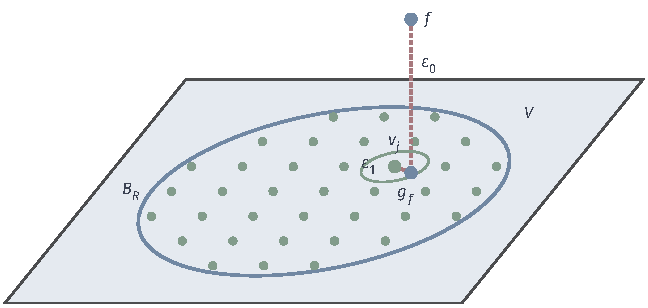
\includegraphics[width=109.7mm]{figures/04-spaces-measures-and-geometry/03-function-spaces/tikz/fcover-two-step/figure.pdf}
  \caption{两步覆盖的几何图景。平面是$n$维子空间$V$，蓝色椭圆是其中半径$R$的闭球，绿点是该球的$\varepsilon_1$网。$f$在$V$之外，先走到$V$中的近似$g_f$（红色虚线，长度不超过$\varepsilon_0$），再走到最近的网点$v_j$（红色实线，长度不超过$\varepsilon_1$）。}
  \label{fig:fcover-two-step}
\end{BookInlineFigure}

图~\ref{fig:fcover-two-step}画出了这两步。定理的两个前提分工明确。$\varepsilon_0$是统一逼近误差，它要求同一个$V$对整类有效，这是“存在$V$，对所有$f$”的量词次序；$R$限定近似所在的有界区域，使有限维覆盖可以进行。

对式~\eqref{eq:fcover-finite-dimensional}取对数，度量熵不超过$n\log(1+2R/\varepsilon_1)$。$n$取代了上一节的节点数，所以有限维表示的度量熵按$n\log(1/\varepsilon_1)$增长。复值函数空间可以看作实空间处理，$n$维复子空间的实维数是$2n$，指数相应换成$2n$。

\paragraph{范数界与系数界}

用范数表述时，界$R$几乎是自动的：若$\lVert f\rVert\leq B$，则$\lVert g_f\rVert\leq B+\varepsilon_0$。但实际存储的是某组基$\varphi_1,\ldots,\varphi_n$下的系数，量化的是系数而不是抽象的子空间元素，这时需要的是系数一致有界。

设$g_\theta=\sum_{i=1}^n\theta_i\varphi_i$，$\lvert\theta_i\rvert\leq\beta$，误差取一致范数，并记$\Lambda=\sup_x\sum_i\lvert\varphi_i(x)\rvert$。逐点估计，得到
\[
 \lVert g_\theta-g_{\theta'}\rVert_\infty\leq\Lambda\max_i\lvert\theta_i-\theta'_i\rvert .
\]
把每个系数量化到间距$2\varepsilon_1/\Lambda$的刻度上，按式~\eqref{eq:fcover-levels}的取法，每个系数有$\lceil\beta\Lambda/\varepsilon_1\rceil$种取值，得到至多$\lceil\beta\Lambda/\varepsilon_1\rceil^n$个代表，每个近似$g_f$与某个代表相差不超过$\varepsilon_1$。

系数界与范数界可以相差很大，差别来自基的选取。这和有限维的斜坐标系一样：两个基向量几乎平行时，同一个向量的坐标可能很大。在$C[0,1]$中取$\varphi_1=1$、$\varphi_2=1+\delta x$（$0<\delta<1$），则
\[
 x=\frac{\varphi_2-\varphi_1}\delta .
\]

函数$x$的一致范数是$1$，在这组基下的系数却是$(-1/\delta,1/\delta)$，$\delta$越小越大。取$\delta=0.01$、$\varepsilon_1=0.1$，用这组基存$x$需要$\beta=100$、$\Lambda=2.01$，每个系数的刻度数是
\[
 \Bigl\lceil\frac{100\cdot2.01}{0.1}\Bigr\rceil=2010 .
\]
而基$(1,x)$下系数只有$(0,1)$，$\beta=1$、$\Lambda=2$，每个系数$\lceil2/0.1\rceil=20$种取值就够。

两组基张成同一个子空间，覆盖数的范数版本不受影响。按系数量化时，几乎线性相关的基会让刻度数膨胀。所以用系数构造覆盖，必须核对系数本身的一致上界，不能只看函数的范数。

\paragraph{正弦级数类的例子}

现在给出一个系数列真正起作用的例子。取$C[0,1]$中的函数类
\begin{equation}
 \mathcal F=\Bigl\{f(x)=\sum_{k\geq1}a_k\sin(k\pi x):\ \sum_{k\geq1}k\lvert a_k\rvert\leq1\Bigr\}.
 \label{eq:fcover-sine-class}
\end{equation}
由于$\sum_k\lvert a_k\rvert\leq1$，级数一致收敛，每个成员都是连续函数。条件$\sum_kk\lvert a_k\rvert\leq1$让靠后的系数整体变小，这正是本节要的“尾部可舍”。

取$V_n$为$\sin(k\pi x)$（$1\leq k\leq n$）张成的子空间，$g_f$为前$n$项部分和。当$k>n$时$\lvert a_k\rvert\leq(k/n)\lvert a_k\rvert$，所以尾项满足
\[
 \lVert f-g_f\rVert_\infty\leq\sum_{k>n}\lvert a_k\rvert\leq\frac1n\sum_{k>n}k\lvert a_k\rvert\leq\frac1n .
\]
部分和本身的范数不超过系数绝对值之和，所以$\lVert g_f\rVert_\infty\leq1$。

用一个具体成员核对。$f(x)=\tfrac12\sin(\pi x)+\tfrac16\sin(3\pi x)$满足$1\cdot\tfrac12+3\cdot\tfrac16=1$，取$n=2$时被舍去的是$\tfrac16\sin(3\pi x)$，误差为$1/6$，不超过$1/n=1/2$。

所以定理~\ref{thm:fcover-finite-dimensional}的前提在$\varepsilon_0=1/n$、$R=1$下成立。给定$\varepsilon$，取$n=\lceil2/\varepsilon\rceil$与$\varepsilon_1=\varepsilon/2$，则$\varepsilon_0+\varepsilon_1\leq\varepsilon$，于是
\begin{equation}
 \log N_{C[0,1]}(\varepsilon,\mathcal F)\leq\Bigl\lceil\frac2\varepsilon\Bigr\rceil\log\Bigl(1+\frac4\varepsilon\Bigr).
 \label{eq:fcover-sine-entropy}
\end{equation}
例如$\varepsilon=1/2$时$n=4$，上界为$4\ln9\approx8.79$；$\varepsilon=0.1$时$n=20$，上界为$20\ln41\approx74.3$。

式~\eqref{eq:fcover-sine-entropy}与上一节一维Lipschitz类的式~\eqref{eq:fcover-entropy-bound}同为$\varepsilon^{-1}\log(1/\varepsilon)$的形式。这不是巧合：逐项求导得$\lvert f'\rvert\leq\pi$，$\mathcal F$本身含于一个Lipschitz类。两种构造从不同的结构出发，一个截取取值列，一个截取系数列，得到同样形式的计数。表~\ref{tab:fcover-two-lists}对比了两条路线。

\begin{BookInlineTable}
  \centering
  \begin{tabular}{@{}lll@{}}
    \toprule
    & 取值列 & 系数列\\
    \midrule
    下标 & 网格节点$v$ & 基函数编号$k$\\
    利用的约束 & 相邻节点相差至多$L/m$ & 舍去的尾部不超过$\varepsilon_0$\\
    有效坐标数 & $(m+1)^d$ & $n$\\
    每个坐标 & $T$个刻度 & 有限维球覆盖\\
    度量熵上界 & 式~\eqref{eq:fcover-entropy-bound} & $n\log(1+2R/\varepsilon_1)$\\
    \bottomrule
  \end{tabular}
  \caption{两条路线对比。两者都把函数看作一列数，都把无穷多个坐标压缩成有限个有效坐标，区别在于压缩所依据的约束。}
  \label{tab:fcover-two-lists}
\end{BookInlineTable}

\paragraph{从多个子空间中选择}

若不要求所有成员共用一个子空间，而允许每个成员从$J$个候选子空间$V_1,\ldots,V_J$中挑选一个（各为$n$维，前提中的$\varepsilon_0$与$R$相同），就对每个候选子空间分别构造覆盖，再取并集：
\begin{equation}
 \log N_E(\varepsilon_0+\varepsilon_1,\mathcal F)\leq\log J+n\log\Bigl(1+\frac{2R}{\varepsilon_1}\Bigr).
 \label{eq:fcover-many-subspaces}
\end{equation}

选择的自由要用$\log J$支付。例如从$D$个固定的基函数中任选$n$个，$J=\binom Dn\leq D^n$，度量熵多出至多$n\log D$。取$D=100$、$n=5$，有$J=75\,287\,520$，$\ln J\approx18.1$，而上界$n\ln D\approx23.0$。

候选子空间的个数必须受控。若候选子空间是一个连续参数族，例如所有平移$\varphi(x-t)$各自张成的一维子空间，$J$为无穷，上面的并集论证就失效，需要另行覆盖参数$t$。怎样构造满足这些前提的有限表示，固定子空间与自适应选择的误差怎样比较，是第~\ref{chap:function-approximation}章的问题。

\section{本章小结}
\label{sec:fcover-summary}

本章开头问：能否预先造一张有限的函数表，使一类函数中的每个成员都在给定精度内有一行与之对应，这张表又需要多少行。用覆盖数表述，前一问是$N(\varepsilon,\mathcal F)$是否对每个$\varepsilon$有限，后一问是它随$\varepsilon$怎样增长。表中的行可以取在环境空间中，也可以要求取在类内，两种约定只差把精度减半。这个问题与为单个函数挑选近似不同：后者的预算可以随成员变化，前者要求一份预算服务整类。答案也依赖距离，同一族指示函数在积分距离下可以有限覆盖，在一致距离下不能。

只限制范数不足以得到有限覆盖。无限维空间的闭球中有彼此远离的序列，$C[0,1]$中越来越陡的帽形函数就是例子。在紧度量空间上，Arzelà--Ascoli判据给出了一致距离下的完整回答：连续函数类全有界、相对紧、一致有界且等度连续三者等价，类自身紧还需闭性。证明的机制是有限化，等度连续让有限个位置代表整个定义域，一致有界让每个位置只有有限种取值记录。紧定义域不能省略，$\mathbb R$上的平移族共用Lipschitz常数，却没有有限覆盖。

把这一机制做成具体构造，就得到计数。对$[0,1]^d$上幅值不超过$M$、Lipschitz常数为$L$的函数，网格误差由$L/m$控制，取值误差由量化间距控制，多线性插值把节点值连成连续的代表。直接计数给出度量熵上界$(\lceil2L/\varepsilon\rceil+1)^d\log\lceil2M/\varepsilon\rceil$；利用相邻节点的约束可以去掉主项中的对数因子，符号隆起的打包集又给出$(L/(6\varepsilon))^d\log2$的下界。维数出现在指数上，幅值只进入对数项。另一条路线是有限维表示：整类若能在同一个$n$维子空间中以误差$\varepsilon_0$统一逼近且近似有界，度量熵就不超过$n\log(1+2R/\varepsilon_1)$；按系数量化时还要核对系数界，允许从多个子空间中选择时要为候选个数付出$\log J$。

本章的结论都是确定性的：给定函数类、距离与精度，代表表是否存在、有多大。把它们用于由随机样本估计函数的问题，还需要另外的概率工具。下一章转向周期函数和全空间函数的频率表示，其中Fourier系数的衰减速度正是本章正弦级数类例子所用的那类条件；怎样构造满足统一逼近前提的有限表示，则在第~\ref{chap:function-approximation}章研究。


\chapter{Fourier变换}
\label{chap:fourier-transform}
\label{chap:orthogonal-expansions-transforms}

一段周期振动可以看成若干个频率的叠加：基频决定音高，各次谐波的强弱决定音色。把函数写成复指数$e^{\mathrm ikx}$的组合，就是为它换上一套频率坐标。在这套坐标下，平移变成乘一个相位因子，求导变成乘频率，卷积变成逐频率相乘，许多在原变量下要做积分的运算化为乘法。问题在于这套坐标对哪些函数有意义、在什么意义下能把函数还原，以及那些运算规则在什么条件下成立。

本章先处理周期函数。第~\ref{sec:fourier-series}节在周期区间上用复指数正交系读出Fourier系数，由完备性得到$L^2$中的展开，再分别核对逐点收敛与一致收敛需要的额外正则性。非周期函数没有离散的谐波，频率要取遍整个实轴，求和变为积分。第~\ref{sec:fourier-l1}节对绝对可积函数定义Fourier变换，研究它的有界性、连续性与高频衰减，再单独回答反演何时成立。

$L^1$中的积分定义有一个缺陷：平方可积的函数未必绝对可积，而能量关系天然属于$L^2$。第~\ref{sec:fourier-l2}节用截断与稠密延拓把变换推广到$L^2$，得到保持范数与内积的反演。第~\ref{sec:fourier-operations}节在固定的函数空间中推导平移、缩放、微分与卷积的变换规则。第~\ref{sec:fourier-discrete}节比较连续频率、周期系数与有限维离散变换这三种表示，说明它们之间的转换需要周期化或取样。

全章固定归一化：周期取$2\pi$，系数带因子$1/(2\pi)$；全空间变换的指数取$e^{-2\pi\mathrm ix\cdot\xi}$，这样反演与能量关系中不出现额外常数。有限项截断或频带截断的逼近误差统一在第~\ref{chap:function-approximation}章研究；用尺度与位置同时组织局部细节的表示，是第~\ref{chap:wavelet-transform}章的小波变换。

\section{Fourier级数}
\label{sec:fourier-series}

在$\mathbb R^n$中取一组标准正交基$q_1,\ldots,q_n$，向量$v$的第$j$个坐标就是内积$a_j=\langle q_j,v\rangle$，并且$v=\sum_ja_jq_j$，$\lVert v\rVert^2=\sum_j\lvert a_j\rvert^2$。第~\ref{chap:function-inner-product-spaces}章把这套做法搬到了Hilbert空间。本节把它用在周期函数上，基取复指数$e^{\mathrm ikx}$，第$k$个基函数在一个周期内恰好转$k$圈，所以坐标记录的是第$k$次振荡的强弱。

先在$L^2$中建立展开，这是类比最直接的部分。然后问部分和在每一点、或在整个周期上一致地趋于什么，这两个问题要用到正交性之外的条件。

\subsection{\texorpdfstring{$L^2$}{L2}中的Fourier展开}
\label{sec:fourier-series-l2}

\paragraph{周期函数与归一化内积}

本节的函数都以$2\pi$为周期。等价地，可以把它看成区间$[-\pi,\pi)$上的函数，并把两个端点粘成一点。记这样的周期区间为$\mathbb T$，积分都在一个周期上进行。平方可积的周期函数组成$L^2(\mathbb T)$，它的元素是几乎处处相等的函数组成的等价类，第~\ref{chap:function-inner-product-spaces}章已证明它是Hilbert空间。

沿用第~\ref{chap:function-inner-product-spaces}章的约定，内积对第二个变量线性。我们在内积前放一个因子$1/(2\pi)$，使常数函数$1$的长度恰好为$1$：
\begin{equation}
\langle f,g\rangle=\frac1{2\pi}\int_{-\pi}^{\pi}\overline{f(x)}\,g(x)\,\mathrm dx .
\label{eq:fourier-circle-inner-product}
\end{equation}
相应的范数是$\lVert f\rVert_2=\langle f,f\rangle^{1/2}$。同样地，$L^1$范数也取平均：
\[
\lVert f\rVert_1=\frac1{2\pi}\int_{-\pi}^{\pi}\lvert f(x)\rvert\,\mathrm dx.
\]

记$e_k(x)=e^{\mathrm ikx}$，$k\in\mathbb Z$。下面验证它们标准正交。当$k=j$时，被积函数恒为$1$，所以$\langle e_j,e_k\rangle=1$。当$k\neq j$时，令$m=k-j\neq0$，直接积分得到
\[
\langle e_j,e_k\rangle=\frac1{2\pi}\int_{-\pi}^{\pi}e^{\mathrm imx}\,\mathrm dx
=\frac{e^{\mathrm im\pi}-e^{-\mathrm im\pi}}{2\pi\mathrm im}.
\]
由于$e^{\mathrm imx}$以$2\pi$为周期，分子中两个端点的值相同，所以
\[
\langle e_j,e_k\rangle=0.
\]
这正是周期性的作用：一个整数圈的旋转，正负部分恰好抵消。

\paragraph{Fourier系数与部分和}

有了标准正交系，第$k$个坐标自然就是与$e_k$的内积。

\begin{definition}[Fourier系数与Fourier级数]
\label{def:fourier-coefficients}
对$f\in L^1(\mathbb T)$，称
\begin{equation}
\widehat f(k)=\frac1{2\pi}\int_{-\pi}^{\pi}f(x)e^{-\mathrm ikx}\,\mathrm dx ,\qquad k\in\mathbb Z
\label{eq:fourier-coefficient}
\end{equation}
为$f$在方向$e_k$上的坐标，称为第$k$个\term{Fourier系数}（Fourier coefficient）。形式级数$\sum_{k\in\mathbb Z}\widehat f(k)e^{\mathrm ikx}$称为$f$的\term{Fourier级数}（Fourier series），它的对称部分和记为
\begin{equation}
S_Nf=\sum_{\lvert k\rvert\leq N}\widehat f(k)\,e_k .
\label{eq:fourier-partial-sum}
\end{equation}
\end{definition}

对$f\in L^2(\mathbb T)$，式~\eqref{eq:fourier-coefficient}就是$\widehat f(k)=\langle e_k,f\rangle$。只要$f$可积，系数就有定义，并且$\lvert\widehat f(k)\rvert\leq\lVert f\rVert_1$。一个周期的长度有限，由Cauchy--Schwarz不等式，$L^2(\mathbb T)\subseteq L^1(\mathbb T)$，所以平方可积函数都有系数。

于是一个函数对应一列坐标$[\ldots,\widehat f(-1),\widehat f(0),\widehat f(1),\ldots]$。下面算一个完整的例子，后面的定理都会回到它。

\begin{example}[方波的坐标]
\label{ex:fourier-square-wave}
取方波：在$(0,\pi)$上$f=1$，在$(-\pi,0)$上$f=-1$，再按$2\pi$周期延拓；在$0$和$\pm\pi$处的取值暂不规定。

$f$是奇函数，所以$\widehat f(0)=0$。对$k\neq0$，把积分分成两段：
\[
\widehat f(k)=\frac1{2\pi}\Bigl(\int_0^{\pi}e^{-\mathrm ikx}\,\mathrm dx-\int_{-\pi}^0e^{-\mathrm ikx}\,\mathrm dx\Bigr).
\]
两段分别积分，并用$e^{\pm\mathrm ik\pi}=(-1)^k$，得到
\[
\int_0^{\pi}e^{-\mathrm ikx}\,\mathrm dx=\frac{1-(-1)^k}{\mathrm ik},\qquad
\int_{-\pi}^0e^{-\mathrm ikx}\,\mathrm dx=\frac{(-1)^k-1}{\mathrm ik}.
\]
代回去，第$k$个系数是
\[
\widehat f(k)=\frac{1-(-1)^k}{\pi\mathrm ik}.
\]
偶数$k$的系数为零，奇数$k$的系数为$2/(\pi\mathrm ik)$，模长为$2/(\pi\lvert k\rvert)$。

把$\pm k$两项配对，括号里出现$2\mathrm i\sin kx$，得到第$k$次（$k$为正奇数）的实形式
\[
\widehat f(k)e^{\mathrm ikx}+\widehat f(-k)e^{-\mathrm ikx}=\frac4{\pi k}\sin kx.
\]
所以前几项是
\[
S_5f(x)=\frac4\pi\Bigl(\sin x+\frac13\sin3x+\frac15\sin5x\Bigr).
\]
\end{example}

图~\ref{fig:fourier-square-coordinates}把这个例子的两种“一列数”并排放在一起。左边是取值，下标是$x$；右边是坐标，下标是$k$。同一个向量换了一组基来记录，三条灰色的正弦波叠加起来，已经勾出方波的轮廓。

\begin{BookInlineFigure}
  \centering
  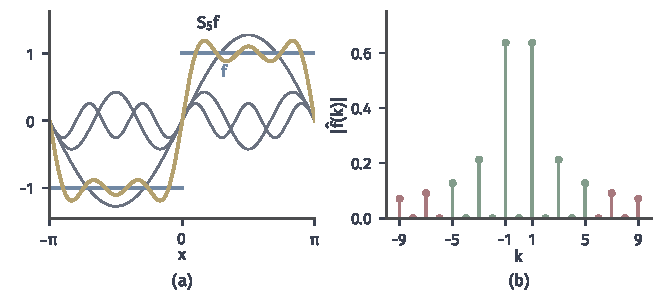
\includegraphics[width=112mm]{figures/04-spaces-measures-and-geometry/03-function-spaces/matplotlib/fourier-square-coordinates/figure.pdf}
  \caption{方波的两种记录方式。(a)蓝色为方波$f$，灰色为$\frac4{\pi}\sin x$、$\frac4{3\pi}\sin3x$、$\frac4{5\pi}\sin5x$三个分量，黄色为它们的和$S_5f$。(b)模长$\lvert\widehat f(k)\rvert$，绿色为$S_5f$保留的坐标（$\lvert k\rvert\leq5$），红色为舍弃的坐标；偶数下标的坐标都是零。}
  \label{fig:fourier-square-coordinates}
\end{BookInlineFigure}

部分和有明确的几何含义。有限组合$\sum_{\lvert k\rvert\leq N}c_ke_k$称为次数不超过$N$的\term{三角多项式}（trigonometric polynomial），它们组成$2N+1$维子空间$\mathcal T_N$。由第~\ref{chap:function-inner-product-spaces}章的有限截断定理，$S_Nf$是$f$在$\mathcal T_N$上的正交投影，也就是$\mathcal T_N$中离$f$最近的元素。同一章的Bessel不等式给出
\[
\sum_{k\in\mathbb Z}\lvert\widehat f(k)\rvert^2\leq\lVert f\rVert_2^2 .
\]

表~\ref{tab:fourier-dictionary}汇总了目前的对应。最后一行是类比失效的地方。

\begin{BookInlineTable}
  \centering
  \begin{tabular}{@{}ll@{}}
    \toprule
    $\mathbb C^n$与标准正交基$q_j$ & $L^2(\mathbb T)$与$e_k=e^{\mathrm ikx}$\\
    \midrule
    坐标$a_j=\langle q_j,v\rangle$ & Fourier系数$\widehat f(k)=\langle e_k,f\rangle$\\
    投影到前几个基向量 & 部分和$S_Nf$\\
    $\sum_j\lvert a_j\rvert^2\leq\lVert v\rVert^2$ & Bessel不等式\\
    $v=\sum_ja_jq_j$，有限和 & $f=\sum_k\widehat f(k)e_k$，$L^2$收敛\\
    $n$个正交向量自动成基 & 无穷多个正交元素未必成基\\
    \bottomrule
  \end{tabular}
  \caption{有限维标准正交基与复指数系的对应。}
  \label{tab:fourier-dictionary}
\end{BookInlineTable}

有限维中，$n$个标准正交向量必定张成全空间。无限维中，数量不能说明问题：从$\{e_k\}$中拿掉$e_0$，剩下的仍是无穷多个标准正交元素，但常数函数$1$与它们全部正交，再也表示不出来。所以写“级数”时还没有断言它收敛，更没有断言它等于$f$。要得到$L^2$中的等式，还需要证明这个系是完备的：与所有$e_k$正交的元素只有零。

\paragraph{Fejér平均}

要证明完备性，一种办法是把$f$写成三角多项式的极限，而这些三角多项式只依赖于$f$的Fourier系数。这样，系数全为零的函数就只能是零。先试部分和$S_Nf$本身。把系数的定义代入式~\eqref{eq:fourier-partial-sum}，交换有限和与积分，再利用周期函数平移不改变一个周期上的积分，得到
\begin{equation}
S_Nf(x)=\frac1{2\pi}\int_{-\pi}^{\pi}f(x-t)D_N(t)\,\mathrm dt ,
\label{eq:fourier-dirichlet-integral}
\end{equation}
其中
\[
D_N(t)=\sum_{\lvert k\rvert\leq N}e^{\mathrm ikt}
\]
称为\term{Dirichlet核}（Dirichlet kernel）。

$D_N$有闭式。当$t\notin2\pi\mathbb Z$时，这是一个公比为$e^{\mathrm it}$的几何级数，首项为$e^{-\mathrm iNt}$，共$2N+1$项：
\[
D_N(t)=e^{-\mathrm iNt}\,\frac{e^{\mathrm i(2N+1)t}-1}{e^{\mathrm it}-1}.
\]
分子分母同乘$e^{-\mathrm it/2}$，分母变成$2\mathrm i\sin(t/2)$，分子变成$2\mathrm i\sin\bigl((N+\tfrac12)t\bigr)$乘同一个相位，相位恰好抵消。于是
\begin{equation}
D_N(t)=\frac{\sin\bigl((N+\tfrac12)t\bigr)}{\sin(t/2)} .
\label{eq:fourier-dirichlet-closed}
\end{equation}

式~\eqref{eq:fourier-dirichlet-integral}是$f$的一种加权平均，但$D_N$的权有正有负。图~\ref{fig:fourier-kernels}(a)是$N=8$的情形，中央峰高$2N+1=17$，两侧的振荡并不随$N$增大而变小，这使得直接估计$S_Nf-f$很困难。

补救办法是取部分和的算术平均。令
\[
\sigma_Nf=\frac1{N+1}\sum_{n=0}^{N}S_nf,
\]
它对应的核是$F_N=\frac1{N+1}\sum_{n=0}^ND_n$，称为\term{Fejér核}（Fejér kernel）。这相当于把振荡的正负部分在不同的$n$之间相互抵消。

下面算$F_N$的闭式。由式~\eqref{eq:fourier-dirichlet-closed}，分子分母都乘$\sin(t/2)$，并用积化和差公式
\[
\sin\bigl((n+\tfrac12)t\bigr)\sin(t/2)=\tfrac12\bigl(\cos nt-\cos(n+1)t\bigr).
\]
对$n=0,\ldots,N$求和时中间项相消，只剩$\tfrac12\bigl(1-\cos(N+1)t\bigr)$，所以
\[
F_N(t)=\frac1{N+1}\,\frac{1-\cos\bigl((N+1)t\bigr)}{2\sin^2(t/2)}.
\]
再用$1-\cos\theta=2\sin^2(\theta/2)$，得到
\begin{equation}
F_N(t)=\frac1{N+1}\Bigl(\frac{\sin\bigl((N+1)t/2\bigr)}{\sin(t/2)}\Bigr)^2 .
\label{eq:fourier-fejer-closed}
\end{equation}

\begin{BookInlineFigure}
  \centering
  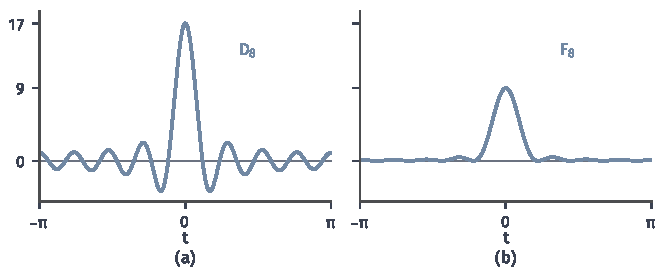
\includegraphics[width=112mm]{figures/04-spaces-measures-and-geometry/03-function-spaces/matplotlib/fourier-kernels/figure.pdf}
  \caption{$N=8$时的两个核，纵轴相同。(a)Dirichlet核$D_8$在$t=0$处高$17$，两侧正负交替。(b)Fejér核$F_8$在$t=0$处高$9$，处处非负，远离原点时几乎为零。}
  \label{fig:fourier-kernels}
\end{BookInlineFigure}

$F_N$有三条性质，恰好是把它当作“集中于原点的权”所需要的，图~\ref{fig:fourier-kernels}(b)可以对照：
\begin{itemize}
\item $F_N\geq0$，这从式~\eqref{eq:fourier-fejer-closed}直接读出；
\item $\frac1{2\pi}\int_{-\pi}^{\pi}F_N=1$，因为每个$D_n$只有常数项$1$对积分有贡献；
\item 对$0<\delta\leq\lvert t\rvert\leq\pi$，$F_N(t)\leq\dfrac1{(N+1)\sin^2(\delta/2)}$，所以质量随$N$增大集中到原点附近。
\end{itemize}

\begin{lemma}[Fejér平均的收敛]
\label{lem:fourier-fejer}
若$f$是连续的周期函数，则$\sigma_Nf$一致收敛到$f$。若$f\in L^2(\mathbb T)$，则$\lVert\sigma_Nf-f\rVert_2\to0$。
\end{lemma}

\begin{proof}
由$F_N$的积分为$1$，把$f(x)$写进积分，得到
\[
\sigma_Nf(x)-f(x)=\frac1{2\pi}\int_{-\pi}^{\pi}\bigl(f(x-t)-f(x)\bigr)F_N(t)\,\mathrm dt.
\]

先看连续的$f$。它在紧区间上一致连续，记
\[
\omega(\delta)=\sup_{\lvert t\rvert<\delta}\sup_x\lvert f(x-t)-f(x)\rvert,
\]
则$\delta\to0$时$\omega(\delta)\to0$。把积分分成$\lvert t\rvert<\delta$与$\delta\leq\lvert t\rvert\leq\pi$两部分。前一部分用$\omega(\delta)$控制差、用积分为$1$控制权；后一部分把差的绝对值放大为$2\lVert f\rVert_\infty$，再用$F_N$的第三条性质。于是
\[
\lvert\sigma_Nf(x)-f(x)\rvert\leq\omega(\delta)+\frac{2\lVert f\rVert_\infty}{(N+1)\sin^2(\delta/2)}.
\]
右边与$x$无关。先取$\delta$使第一项小，再令$N$充分大使第二项小，即得一致收敛。

再看$f\in L^2(\mathbb T)$。由前两条性质，$\frac1{2\pi}F_N(t)\,\mathrm dt$是一个周期上的概率测度。对它用Cauchy--Schwarz不等式，得到
\[
\lvert\sigma_Nf(x)-f(x)\rvert^2\leq\frac1{2\pi}\int_{-\pi}^{\pi}\lvert f(x-t)-f(x)\rvert^2F_N(t)\,\mathrm dt.
\]
对$x$按归一化测度积分，并用Tonelli定理交换次序。记平移$(\tau_tf)(x)=f(x-t)$，于是
\[
\lVert\sigma_Nf-f\rVert_2^2\leq\frac1{2\pi}\int_{-\pi}^{\pi}\lVert\tau_tf-f\rVert_2^2\,F_N(t)\,\mathrm dt.
\]
同样分成$\lvert t\rvert<\delta$与其余部分，并用$\lVert\tau_tf-f\rVert_2\leq2\lVert f\rVert_2$。这样只需再说明$t\to0$时$\lVert\tau_tf-f\rVert_2\to0$。

这一平移连续性分三步得到。第~\ref{chap:smoothing-weak-derivatives}章证明了$\mathbb R$上的可积函数$F$满足$\int\lvert F(x-h)-F(x)\rvert\,\mathrm dx\to0$。对周期函数$f$与$\lvert h\rvert\leq\pi$，取$F=f\mathbf 1_{[-2\pi,2\pi]}$，在$x\in[-\pi,\pi]$上$F(x-h)=f(x-h)$，所以周期情形的$L^1$平移连续性成立。

若还有$\lvert f\rvert\leq n$，则
\[
\lvert\tau_hf-f\rvert^2\leq2n\,\lvert\tau_hf-f\rvert,
\]
所以有界函数的$L^2$平移连续性成立。

对一般的$f\in L^2(\mathbb T)$，取$f_n=f\mathbf 1_{\{\lvert f\rvert\leq n\}}$。由控制收敛定理，$\lVert f-f_n\rVert_2\to0$。平移不改变周期函数的范数，所以
\[
\lVert\tau_hf-f\rVert_2\leq2\lVert f-f_n\rVert_2+\lVert\tau_hf_n-f_n\rVert_2.
\]
先取$n$使第一项小，再令$h\to0$，第二项趋于零。
\end{proof}

\paragraph{完备性与Parseval关系}

$\sigma_Nf$完全由Fourier系数决定，这正是证明完备性所需要的。

\begin{theorem}[$L^2$中的Fourier展开]
\label{thm:fourier-series-l2}
$\{e_k\}_{k\in\mathbb Z}$是$L^2(\mathbb T)$的完备标准正交系。因此对每个$f\in L^2(\mathbb T)$，$\lVert S_Nf-f\rVert_2\to0$，并且
\begin{equation}
\begin{gathered}
\frac1{2\pi}\int_{-\pi}^{\pi}\lvert f(x)\rvert^2\,\mathrm dx=\sum_{k\in\mathbb Z}\lvert\widehat f(k)\rvert^2 ,\\
\langle f,g\rangle=\sum_{k\in\mathbb Z}\overline{\widehat f(k)}\,\widehat g(k) .
\end{gathered}
\label{eq:fourier-series-parseval}
\end{equation}
\end{theorem}

\begin{proof}
设$f\in L^2(\mathbb T)$与每个$e_k$正交，即全部$\widehat f(k)=0$。则每个$S_nf=0$，从而$\sigma_Nf=0$。由引理~\ref{lem:fourier-fejer}，$\sigma_Nf\to f$于$L^2$，所以$f=0$。完备标准正交系的范数收敛展开、Parseval等式及内积公式，由第~\ref{chap:function-inner-product-spaces}章的正交展开定理给出。
\end{proof}

式~\eqref{eq:fourier-series-parseval}就是无限维的勾股定理：一个周期上的平均能量等于各坐标模平方之和，本章称为Parseval关系。截断误差也由它读出，投影与残差正交，所以
\begin{equation}
\lVert f-S_Nf\rVert_2^2=\sum_{\lvert k\rvert>N}\lvert\widehat f(k)\rvert^2 .
\label{eq:fourier-series-truncation}
\end{equation}

结合第~\ref{chap:function-inner-product-spaces}章的结论，$f\mapsto(\widehat f(k))_{k\in\mathbb Z}$是$L^2(\mathbb T)$到$\ell^2(\mathbb Z)$的保持内积的双射。在$L^2$的意义下，“函数是一列坐标”这句话是严格成立的。

用方波核对一下。左边的平均能量为$1$，右边只有奇数$k$有贡献，每个模平方为$4/(\pi^2k^2)$，$\pm k$各一项，所以
\[
1=2\sum_{j\geq0}\frac{4}{\pi^2(2j+1)^2}.
\]
整理后得到一个级数的值：
\[
\sum_{j\geq0}\frac1{(2j+1)^2}=\frac{\pi^2}8 .
\]

截断误差也可以逐项算出。前几项的平方和分别是
\[
\frac8{\pi^2}\approx0.8106,\qquad
\frac8{\pi^2}\Bigl(1+\frac19\Bigr)\approx0.9006,\qquad
\frac8{\pi^2}\Bigl(1+\frac19+\frac1{25}\Bigr)\approx0.9331.
\]
由式~\eqref{eq:fourier-series-truncation}，$\lVert f-S_Nf\rVert_2^2$在$N=1,3,5$时分别约为$0.1894$、$0.0994$、$0.0669$。每增加一个坐标，误差平方恰好减少该坐标的模平方，已经算好的系数不必修改，这是正交基的好处。系数的衰减怎样决定误差的速度，留到第~\ref{chap:function-approximation}章研究。

\paragraph{实形式与一般周期}

实值函数也常用正弦与余弦展开。若$f$为实值，对式~\eqref{eq:fourier-coefficient}取共轭得到$\widehat f(-k)=\overline{\widehat f(k)}$。把$\pm k$两项配对，就得到实形式：
\[
f\sim\frac{a_0}2+\sum_{k\geq1}\bigl(a_k\cos kx+b_k\sin kx\bigr),
\]
其中
\[
a_k=\frac1\pi\int_{-\pi}^{\pi}f(x)\cos kx\,\mathrm dx,\qquad
b_k=\frac1\pi\int_{-\pi}^{\pi}f(x)\sin kx\,\mathrm dx.
\]
两套系数的关系是
\[
\widehat f(0)=\frac{a_0}2,\qquad\widehat f(k)=\frac{a_k-\mathrm ib_k}2\quad(k\geq1).
\]
相应地，Parseval关系写成
\[
\frac1{2\pi}\int_{-\pi}^{\pi}\lvert f\rvert^2=\frac{a_0^2}4+\frac12\sum_{k\geq1}(a_k^2+b_k^2).
\]

两种写法表示同一个展开，实形式中的$1/\pi$与$1/2$都来自配对。方波的实系数是$a_k=0$，奇数$k$时$b_k=4/(\pi k)$，与例~\ref{ex:fourier-square-wave}一致。这相当于把同一组坐标换成实的基$1,\sqrt2\cos kx,\sqrt2\sin kx$来写，只是常数放的位置不同。

若周期是$T$而不是$2\pi$，令$x=2\pi t/T$即可化归本节情形。这时系数为
\begin{equation}
c_k=\frac1T\int_0^Tf(t)\,e^{-2\pi\mathrm ikt/T}\,\mathrm dt ,
\label{eq:fourier-period-T}
\end{equation}
第$k$个基函数的频率是单位长度内$k/T$圈。周期越长，相邻频率越靠近，这一点在下一节开头会用到。

\paragraph{系数描述的是等价类}

类比还有一个需要注意的地方。Fourier系数是积分，改变$f$在一个零测集上的值不改变任何坐标。所以坐标记录的不是一张逐点的取值表，而是$L^2(\mathbb T)$中的一个等价类。定理~\ref{thm:fourier-series-l2}中的展开是范数意义下的等式，不是逐点等式。

例~\ref{ex:fourier-square-wave}中没有规定方波在$0$和$\pm\pi$处的取值，原因就在这里：无论在这些点赋什么值，算出来的系数都一样，$\pi^2/8$这个结果也一样。要讨论$S_Nf$在某一点的值，必须另外加条件，这是下一小节的内容。

\subsection{点态收敛}
\label{sec:fourier-series-pointwise}

$L^2$收敛控制的是一个周期上的平均平方误差，它不告诉我们部分和在某个给定点处是否收敛。连续性也不够：du Bois-Reymond构造过连续周期函数，其Fourier级数在某一点发散，构造较长，读者可查阅Fourier分析的教材。所以逐点结论必须对$f$加上比连续更强的局部条件，本小节使用分段$C^1$条件。

\paragraph{Riemann--Lebesgue引理}

逐点收敛的证明最终要说明一个高频振荡积分趋于零。直观上，$g(t)e^{-\mathrm i\lambda t}$在长度为$\pi/\lambda$的小段上一正一负，而$g$在这么短的距离上几乎不变，正负两部分几乎抵消。这件事对任何可积函数都成立。

\begin{lemma}[Riemann--Lebesgue引理]
\label{lem:fourier-riemann-lebesgue}
若$g\in L^1(\mathbb R)$，则$\lvert\lambda\rvert\to\infty$时
\begin{equation}
\int_{\mathbb R}g(t)e^{-\mathrm i\lambda t}\,\mathrm dt\to0 .
\label{eq:fourier-riemann-lebesgue}
\end{equation}
特别地，$\int g(t)\sin(\lambda t)\,\mathrm dt\to0$；对$f\in L^1(\mathbb T)$，$\lvert k\rvert\to\infty$时$\widehat f(k)\to0$。
\end{lemma}

\begin{proof}
把式~\eqref{eq:fourier-riemann-lebesgue}左边的积分记为$I(\lambda)$，$\lambda\neq0$。作换元$t\mapsto t+\pi/\lambda$，并用$e^{-\mathrm i\pi}=-1$，得到
\[
I(\lambda)=-\int_{\mathbb R}g(t+\pi/\lambda)\,e^{-\mathrm i\lambda t}\,\mathrm dt.
\]
把它与原式相加再取模，得到
\[
2\lvert I(\lambda)\rvert\leq\int_{\mathbb R}\lvert g(t)-g(t+\pi/\lambda)\rvert\,\mathrm dt.
\]
由第~\ref{chap:smoothing-weak-derivatives}章的平移积分连续性，右边在$\lvert\lambda\rvert\to\infty$时趋于零。对$\lambda$取实部虚部即得正弦情形。周期情形把$f$在一个周期外置零，再取$\lambda=k$。
\end{proof}

对$L^2$函数，坐标趋于零可以由Bessel不等式读出，因为平方可和的序列必趋于零。引理的新内容在于它只要求可积，而$L^1(\mathbb T)$函数的坐标不必平方可和。它也不给出趋于零的速度：方波的系数按$1/\lvert k\rvert$衰减，后面会看到更光滑的函数衰减得更快。

\paragraph{分段$C^1$函数的Dirichlet定理}

称周期函数$f$为分段$C^1$，是指在一个周期$[-\pi,\pi]$中有有限个分点，使$f$在每个开子区间上连续可微，并且$f$与$f'$在每个子区间端点处有单侧极限。于是在每一点$x$都存在单侧极限$f(x+)$与$f(x-)$，它们在连续点相等，在跳跃点不等。方波是最典型的例子。

\begin{theorem}[Dirichlet定理]
\label{thm:fourier-dirichlet}
设$f$是分段$C^1$的$2\pi$周期函数，则对每个$x\in\mathbb R$，
\begin{equation}
\lim_{N\to\infty}S_Nf(x)=\frac{f(x+)+f(x-)}2 .
\label{eq:fourier-dirichlet-limit}
\end{equation}
特别地，在$f$的连续点，$S_Nf(x)\to f(x)$。
\end{theorem}

\begin{proof}
$D_N$是偶函数，所以式~\eqref{eq:fourier-dirichlet-integral}可以按$t>0$与$t<0$合并为
\[
S_Nf(x)=\frac1{2\pi}\int_0^{\pi}\bigl[f(x+t)+f(x-t)\bigr]D_N(t)\,\mathrm dt.
\]
又由$D_N$的积分得$\frac1{2\pi}\int_0^{\pi}D_N=\frac12$，因此可以把左右极限的平均写进同一个积分。记
\[
h(t)=f(x+t)-f(x+)+f(x-t)-f(x-),
\]
并利用式~\eqref{eq:fourier-dirichlet-closed}，得到
\[
S_Nf(x)-\frac{f(x+)+f(x-)}2=\frac1{2\pi}\int_0^{\pi}\frac{h(t)}{\sin(t/2)}\sin\bigl((N+\tfrac12)t\bigr)\,\mathrm dt.
\]
只需说明$g(t)=h(t)/\sin(t/2)$在$(0,\pi)$上可积，然后对$g\mathbf 1_{(0,\pi)}$用引理~\ref{lem:fourier-riemann-lebesgue}。

取$t_0>0$，小于$x$到两侧最近分点的距离。在$(x,x+t_0)$上$f$连续可微，$f'$有单侧极限，所以$\lvert f'\rvert\leq C$。对$0<s<t<t_0$用中值定理，得到$\lvert f(x+t)-f(x+s)\rvert\leq C(t-s)$。令$s\to0^+$，得到
\[
\lvert f(x+t)-f(x+)\rvert\leq Ct.
\]
左侧同理。又$0\leq t\leq\pi$时$\sin(t/2)\geq t/\pi$，所以$g$在$(0,t_0)$上有界。在$[t_0,\pi]$上，$\sin(t/2)\geq\sin(t_0/2)>0$，而$f$有界，$g$也有界。因此$g$可积，引理给出右边趋于零。
\end{proof}

\paragraph{连续点、跳跃点与等价类}

定理把每一点分成两类，用方波可以逐一核对。取连续点$x=\pi/2$，这时$\sin(k\pi/2)$对$k=1,3,5,\ldots$依次为$1,-1,1,\ldots$，所以
\[
S_Nf\Bigl(\frac\pi2\Bigr)=\frac4\pi\Bigl(1-\frac13+\frac15-\cdots\Bigr).
\]
$N=1,3,5,7$时的值依次约为$1.273$、$0.849$、$1.104$、$0.922$，在$f(\pi/2)=1$的两侧摆动着收敛。

再取跳跃点$x=0$。每个$\sin(k\cdot0)=0$，所以$S_Nf(0)=0$对一切$N$成立，这正是左右极限的平均$(1+(-1))/2$。无论在$0$处给方波赋什么值，极限都是$0$：单点赋值既不进入系数，也不进入单侧极限。

与$L^2$展开相比，这里多用了$x$两侧的单侧Lipschitz估计，它来自分段$C^1$假设，使$g$在$t=0$附近可积；Riemann--Lebesgue引理本身只需要可积性。证明还显示了收敛的局部性：$g$只在$x$附近需要特别的估计，远离$x$处只用了有界性。$L^2$收敛不能代替这里的局部条件，因为它允许在零测集上任意修改函数，而逐点问题恰恰关心单个点。

\subsection{一致收敛}
\label{sec:fourier-series-uniform}

点态收敛允许不同点以不同速度收敛，一致收敛则要求整个周期上的最大误差趋于零。一个简单的充分条件是坐标绝对可和，而坐标衰减的速度由函数的光滑性控制。

\paragraph{分部积分与系数衰减}

对连续可微的周期函数，分部积分把求导转到坐标上。在$\widehat{f'}(k)$的定义中分部积分，得到
\[
\widehat{f'}(k)=\frac1{2\pi}\Bigl[f(x)e^{-\mathrm ikx}\Bigr]_{-\pi}^{\pi}+\frac{\mathrm ik}{2\pi}\int_{-\pi}^{\pi}f(x)e^{-\mathrm ikx}\,\mathrm dx.
\]
$f$与$e^{-\mathrm ikx}$都以$2\pi$为周期，边界项为零，所以
\begin{equation}
\widehat{f'}(k)=\mathrm ik\,\widehat f(k).
\label{eq:fourier-series-derivative}
\end{equation}
求导在这组坐标下是对角矩阵$\operatorname{diag}(\mathrm ik)$。这一步依赖周期性：若$f(\pi)\neq f(-\pi)$，边界项不为零。

\begin{theorem}[$C^2$函数的一致收敛]
\label{thm:fourier-uniform}
设$f$是二次连续可微的$2\pi$周期函数。则对$k\neq0$有
\begin{equation}
\lvert\widehat f(k)\rvert\leq\frac{\lVert f''\rVert_\infty}{k^2},
\label{eq:fourier-c2-coefficient}
\end{equation}
$\sum_k\lvert\widehat f(k)\rvert<\infty$，并且$S_Nf$一致收敛到$f$，
\begin{equation}
\sup_x\lvert f(x)-S_Nf(x)\rvert\leq\frac{2\lVert f''\rVert_\infty}{N},\qquad N\geq1 .
\label{eq:fourier-c2-uniform-error}
\end{equation}
\end{theorem}

\begin{proof}
用式~\eqref{eq:fourier-series-derivative}两次，得到$\widehat{f''}(k)=-k^2\widehat f(k)$。而$\widehat{f''}(k)$的模不超过$\lVert f''\rVert_1\leq\lVert f''\rVert_\infty$，这给出系数估计。

由$\sum_{k\neq0}k^{-2}<\infty$，Weierstrass判别法说明$S_Nf$一致收敛到某个连续函数$h$。一致收敛蕴含$L^2$收敛，而定理~\ref{thm:fourier-series-l2}说明$S_Nf\to f$于$L^2$，所以$h=f$几乎处处。两个连续函数若在某点不等，就在该点的一个邻域内不等，邻域的测度为正，所以$h=f$处处成立。

误差估计来自尾部求和。对每个$x$，误差不超过被舍弃坐标的模之和：
\[
\lvert f(x)-S_Nf(x)\rvert\leq\sum_{\lvert k\rvert>N}\lvert\widehat f(k)\rvert.
\]
由式~\eqref{eq:fourier-c2-coefficient}，只需估计$k^{-2}$的尾部和：
\[
\sum_{\lvert k\rvert>N}\frac1{k^2}=2\sum_{k>N}\frac1{k^2}\leq2\int_N^\infty\frac{\mathrm dt}{t^2}=\frac2N.
\]
乘上$\lVert f''\rVert_\infty$，就是式~\eqref{eq:fourier-c2-uniform-error}。
\end{proof}

$C^2$只是一个方便的充分条件，连续可微就已足够。由式~\eqref{eq:fourier-series-derivative}与Cauchy--Schwarz不等式，
\[
\sum_{k\neq0}\lvert\widehat f(k)\rvert=\sum_{k\neq0}\frac{\lvert\widehat{f'}(k)\rvert}{\lvert k\rvert}
\leq\lVert f'\rVert_2\Bigl(\sum_{k\neq0}\frac1{k^2}\Bigr)^{1/2},
\]
这里用到$f'$的Parseval关系。

不必处处可导。周期延拓的$\lvert x\rvert$（三角波）在$0$与$\pm\pi$处有尖点，分部积分得到它的系数：
\[
\widehat f(0)=\frac\pi2,\qquad
\widehat f(k)=\frac{(-1)^k-1}{\pi k^2}\quad(k\neq0).
\]
奇数$k$时$\widehat f(k)=-2/(\pi k^2)$，偶数$k\neq0$时为零，绝对可和，所以部分和一致收敛，极限与$f$处处相等的论证同上。

在$x=0$处取值，右边是$\pi/2$减去正数项，得到
\[
0=\frac\pi2-\frac4\pi\sum_{j\geq0}\frac1{(2j+1)^2},
\]
这与方波的Parseval关系给出的$\pi^2/8$一致。逐项算，$N=1,3,5,9$时$S_Nf(0)$依次约为$0.298$、$0.156$、$0.105$、$0.064$，趋于$f(0)=0$。

比较两个例子。方波有跳跃，系数按$1/\lvert k\rvert$衰减，不绝对可和；三角波连续，只有尖点，系数按$1/k^2$衰减，绝对可和。函数越光滑，高频坐标越小。

\paragraph{三种误差的比较}

三种收敛方式衡量的是不同的误差。一致误差$\sup_x\lvert f-S_Nf\rvert$控制每一点，因而控制逐点误差。由$\lVert\cdot\rVert_2\leq\sup\lvert\cdot\rvert$，它也控制$L^2$误差。反过来，$L^2$误差小只说明误差大的地方测度小，逐点收敛也可以在不同点有不同速度。

跳跃函数不能获得一致收敛。部分和$S_Nf$是三角多项式，处处连续；一致收敛的连续函数列的极限连续，可参考\BookChapterRef{chap:limits-continuity}{卷一第5章“极限与连续”}。方波在$0$处跳跃，所以$S_Nf$不可能一致收敛到任何与方波几乎处处相等的函数。

具体的情形可以算出来。取$N=2n-1$，对$S_Nf$求导，用几何级数求和得
\[
(S_Nf)'(x)=\frac4\pi\sum_{j=1}^n\cos\bigl((2j-1)x\bigr)=\frac2\pi\cdot\frac{\sin 2nx}{\sin x}.
\]
所以在$x>0$一侧，第一个峰出现在$x=\pi/(2n)$。把这一点代入$S_Nf$，并记$x_j=(2j-1)\pi/(2n)$，有$\frac1{2j-1}=\frac{\pi}{2n\,x_j}$，于是
\[
S_Nf\Bigl(\frac\pi{2n}\Bigr)=\frac2\pi\sum_{j=1}^n\frac{\sin x_j}{x_j}\cdot\frac\pi n.
\]
右边是$\sin u/u$在$[0,\pi]$上步长$\pi/n$的中点Riemann和，所以$n\to\infty$时
\[
S_Nf\Bigl(\frac\pi{2n}\Bigr)\to\frac2\pi\int_0^\pi\frac{\sin u}{u}\,\mathrm du\approx1.179.
\]
这就是\term{Gibbs现象}（Gibbs phenomenon）：跳跃附近的部分和总要越过跳跃高度，超出约$0.179$，即跳跃幅度$2$的约$9\%$，而峰的位置随$N$增大向跳跃点收缩。$N=9,25,81$时峰值依次约为$1.182$、$1.180$、$1.179$。

\begin{BookInlineFigure}
  \centering
  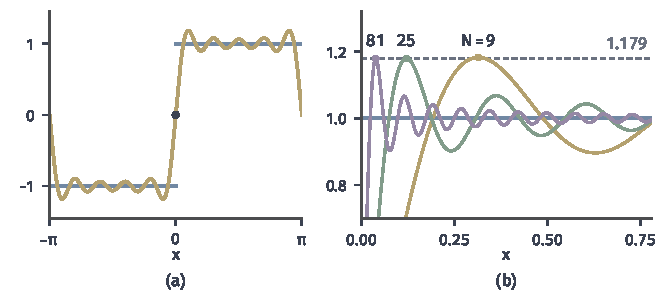
\includegraphics[width=112mm]{figures/04-spaces-measures-and-geometry/03-function-spaces/matplotlib/fourier-gibbs/figure.pdf}
  \caption{方波的Gibbs现象。蓝色为方波。(a)$N=9$的部分和（黄色），在跳跃点$0$处取值$0$（黑点）。(b)$x>0$一侧的放大图，黄、绿、紫分别为$N=9,25,81$，圆点是各自的第一个峰，都接近虚线$1.179$，峰随$N$增大靠近跳跃点。}
  \label{fig:fourier-gibbs}
\end{BookInlineFigure}

图~\ref{fig:fourier-gibbs}(b)说明这与定理~\ref{thm:fourier-dirichlet}并不矛盾。固定一个$x>0$，峰迟早越过它，之后$S_Nf(x)$趋于$1$；只是越靠近跳跃点，收敛越晚，所以最大误差始终不小。三种误差在方波上的表现是：$L^2$误差趋于零，每个固定点的误差趋于零，而一致误差不趋于零。

\section{\texorpdfstring{$L^1$}{L1}中的Fourier变换}
\label{sec:fourier-l1}

非周期函数不能在一个周期上读坐标，但上一节末尾已经提示了办法：周期$T$越长，频率$k/T$越密。对定义在整个$\mathbb R^d$上的函数，频率应当取遍$\mathbb R^d$，对整数$k$的求和换成对频率$\xi$的积分。向量的下标从整数连成了整个空间，这是类比的又一次推广，也是它开始变得不严格的地方。

本节先在绝对可积函数上建立变换本身，再单独回答怎样从频率函数还原原函数。

\subsection{Fourier变换的基本性质}
\label{sec:fourier-l1-properties}

\paragraph{定义与归一化}

先用一个周期很长的函数看看下标是怎样连起来的。设$f$是实轴上的可积函数，支撑在$[-T/2,T/2]$内，把它按$T$周期延拓。由式~\eqref{eq:fourier-period-T}，它的系数$c_k$乘$T$之后是
\[
Tc_k=\int_{-T/2}^{T/2}f(x)\,e^{-2\pi\mathrm i(k/T)x}\,\mathrm dx .
\]
只要$T$足够大，右边的积分就不再依赖$T$，它只依赖频率$\xi=k/T$，是同一个函数$\xi\mapsto\int f(x)e^{-2\pi\mathrm ix\xi}\,\mathrm dx$在格点$k/T$上的取值。

取方框$B=\mathbf 1_{[-1/2,1/2]}$算一个具体的值。取$T=2$、$k=1$，频率是$\xi=1/2$，于是
\[
2c_1=\int_{-1/2}^{1/2}e^{-\mathrm i\pi x}\,\mathrm dx=\frac{\sin(\pi/2)}{\pi/2}=\frac2\pi\approx0.637.
\]
图~\ref{fig:fourier-series-to-transform}画出$T=2,4,8$时的全部$Tc_k$：它们落在同一条曲线上，$T$每增大一倍，取样点就密一倍。

\begin{BookInlineFigure}
  \centering
  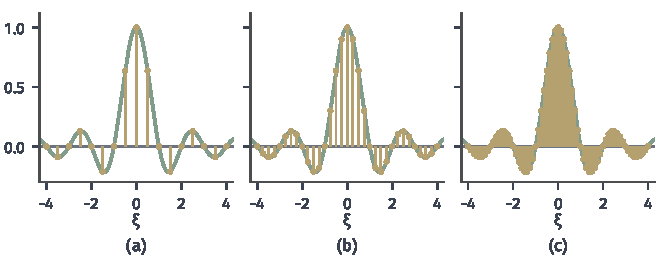
\includegraphics[width=112mm]{figures/04-spaces-measures-and-geometry/03-function-spaces/matplotlib/fourier-series-to-transform/figure.pdf}
  \caption{周期增大时系数连成曲线。方框$B$按周期$T$延拓，黄色竖线为$Tc_k$，位于频率$k/T$处。(a)$T=2$。(b)$T=4$。(c)$T=8$。绿色曲线是极限对象$\sin(\pi\xi)/(\pi\xi)$，三幅图中相同。}
  \label{fig:fourier-series-to-transform}
\end{BookInlineFigure}

展开式也随之变形。把$c_k$代入周期$T$的Fourier级数，得到
\[
f(x)=\sum_{k\in\mathbb Z}\Bigl(\int f(y)e^{-2\pi\mathrm i(k/T)y}\,\mathrm dy\Bigr)\,e^{2\pi\mathrm i(k/T)x}\cdot\frac1T .
\]
右边是一个频率步长为$1/T$的Riemann和。$T\to\infty$时，它的形式极限是对$\xi$的积分。这只是启发，下面的定义和证明不依赖这个极限过程。

对$x,\xi\in\mathbb R^d$，记$x\cdot\xi=\sum_ix_i\xi_i$。函数$x\mapsto e^{2\pi\mathrm ix\cdot\xi}$沿方向$\xi/\lvert\xi\rvert$每前进$1/\lvert\xi\rvert$就转一圈，所以$\lvert\xi\rvert$是单位长度内的圈数，这样的函数称为平面波。

\begin{definition}[Fourier变换]
\label{def:fourier-transform-l1}
对$f\in L^1(\mathbb R^d)$，定义它的\term{Fourier变换}（Fourier transform）为
\begin{equation}
\widehat f(\xi)=\int_{\mathbb R^d}f(x)e^{-2\pi\mathrm ix\cdot\xi}\,\mathrm dx ,\qquad\xi\in\mathbb R^d .
\label{eq:fourier-transform-l1}
\end{equation}
\end{definition}

由于指数因子的模恒为$1$，可积性保证积分对每个$\xi$都存在，并且改变$f$在零测集上的值不影响结果。所以$\widehat f$是一个在每个频率处都有确定值的函数，这一点到$L^2$情形会改变。

类比在这里要打一个折扣。式~\eqref{eq:fourier-transform-l1}形式上是“与平面波作内积”，但平面波的模恒为$1$，在$\mathbb R^d$上既不可积也不平方可积，它们不是$L^2(\mathbb R^d)$中的元素，更谈不上构成正交基。可以把$\widehat f(\xi)$想成下标为$\xi$的坐标，但一切结论都要直接证明，不能照搬Hilbert空间的展开定理。

指数中的$2\pi$是一种约定。另一种常见写法用角频率$\omega=2\pi\xi$，把指数换成$e^{-\mathrm ix\cdot\omega}$，所得函数记为$F(\omega)$，两者只差自变量的伸缩，$F(\omega)=\widehat f(\omega/2\pi)$。约定不改变任何结论，只改变反演与能量公式中的常数；本章始终采用定义中的写法，第~\ref{sec:fourier-l2}节末尾给出常数的对照。

\paragraph{有界性、连续性与高频衰减}

和周期情形一样，可积性已经足以给出变换的几条基本性质。

\begin{theorem}[$L^1$上Fourier变换的基本性质]
\label{thm:fourier-l1-properties}
设$f,g\in L^1(\mathbb R^d)$，$a,b\in\mathbb C$。则
\begin{enumerate}
\item $\widehat{af+bg}=a\widehat f+b\widehat g$，且$\lVert\widehat f\rVert_\infty\leq\lVert f\rVert_1$；
\item $\widehat f$在$\mathbb R^d$上连续；
\item $\lvert\xi\rvert\to\infty$时$\widehat f(\xi)\to0$。
\end{enumerate}
\end{theorem}

\begin{proof}
线性来自积分的线性。有界性来自
\[
\lvert\widehat f(\xi)\rvert\leq\int_{\mathbb R^d}\lvert f(x)e^{-2\pi\mathrm ix\cdot\xi}\rvert\,\mathrm dx=\lVert f\rVert_1.
\]

连续性：若$\xi_n\to\xi$，被积函数逐点收敛到$f(x)e^{-2\pi\mathrm ix\cdot\xi}$，并被可积函数$\lvert f\rvert$控制。由控制收敛定理，$\widehat f(\xi_n)\to\widehat f(\xi)$。

高频衰减与引理~\ref{lem:fourier-riemann-lebesgue}的证明相同。对$\xi\neq0$取
\[
h=\frac{\xi}{2\lvert\xi\rvert^2},
\]
则$e^{-2\pi\mathrm ih\cdot\xi}=e^{-\pi\mathrm i}=-1$。作换元$x\mapsto x+h$，得到
\[
\widehat f(\xi)=-\int_{\mathbb R^d}f(x+h)\,e^{-2\pi\mathrm ix\cdot\xi}\,\mathrm dx.
\]
与原式相加再取模，得到
\[
2\lvert\widehat f(\xi)\rvert\leq\int_{\mathbb R^d}\lvert f(x)-f(x+h)\rvert\,\mathrm dx.
\]
$\lvert\xi\rvert\to\infty$时$\lvert h\rvert=1/(2\lvert\xi\rvert)\to0$，由第~\ref{chap:smoothing-weak-derivatives}章的平移积分连续性，右边趋于零。
\end{proof}

于是$f\mapsto\widehat f$把$L^1(\mathbb R^d)$线性地映到在无穷远处趋于零的有界连续函数中，而且不增加相应的范数。第3条也称为Riemann--Lebesgue引理。它不给出衰减速度，速度与$f$的光滑性有关，第~\ref{sec:fourier-operations}节的微分规则会给出具体联系。

\paragraph{三个例子}

先算两个一维例子。第一个是中心方框$B=\mathbf 1_{[-1/2,1/2]}$。直接积分，对$\xi\neq0$有
\begin{equation}
\widehat B(\xi)=\int_{-1/2}^{1/2}e^{-2\pi\mathrm ix\xi}\,\mathrm dx=\frac{\sin(\pi\xi)}{\pi\xi},
\label{eq:fourier-box}
\end{equation}
并且$\widehat B(0)=1$。零点在非零整数处，例如$\widehat B(1/2)=2/\pi$，与上面周期化时算出的$2c_1$相同。

$\widehat B$连续，在无穷远处趋于零，但只按$1/\lvert\xi\rvert$衰减，在$\mathbb R$上不绝对可积。事实上，在每个区间$[n,n+1]$（$n\geq1$）上，分母不超过$\pi(n+1)$，而$\lvert\sin\pi\xi\rvert$在长度为$1$的区间上的积分是$2/\pi$，所以
\[
\int_n^{n+1}\frac{\lvert\sin\pi\xi\rvert}{\pi\lvert\xi\rvert}\,\mathrm d\xi\geq\frac{2}{\pi^2(n+1)}.
\]
对$n$求和，调和级数发散。

第二个例子是双边指数$f(x)=e^{-\lvert x\rvert}$。把积分分成$x>0$与$x<0$两段，第二段作换元$x\mapsto-x$，得到
\[
\widehat f(\xi)=\int_0^\infty e^{-x(1+2\pi\mathrm i\xi)}\,\mathrm dx+\int_0^\infty e^{-x(1-2\pi\mathrm i\xi)}\,\mathrm dx.
\]
每段都是指数积分，所以
\[
\widehat f(\xi)=\frac1{1+2\pi\mathrm i\xi}+\frac1{1-2\pi\mathrm i\xi}.
\]
通分，得到
\begin{equation}
\widehat f(\xi)=\frac{2}{1+4\pi^2\xi^2}.
\label{eq:fourier-double-exponential}
\end{equation}
它按$1/\xi^2$衰减，是可积的。检验一下：$\widehat f(0)=2$，正是$\int e^{-\lvert x\rvert}\,\mathrm dx$的值。

第三个例子是Gauss函数$G(x)=e^{-\pi\lvert x\rvert^2}$，它的变换就是它自己：$\widehat G=G$。先看$d=1$。由极坐标（二重积分的换元可参考\BookChapterRef{chap:region-integrals}{卷二第24章“区域积分”}），
\[
\Bigl(\int_{\mathbb R}e^{-\pi x^2}\,\mathrm dx\Bigr)^2=\int_0^{2\pi}\int_0^\infty e^{-\pi r^2}r\,\mathrm dr\,\mathrm d\theta=1,
\]
所以$\int e^{-\pi x^2}\,\mathrm dx=1$。

再令$\varphi(\xi)=\widehat G(\xi)$。由于$\lvert x\rvert e^{-\pi x^2}$可积，可以在积分号下对$\xi$求导（第~\ref{chap:integration}章的含参积分求导条件）。注意$(e^{-\pi x^2})'=-2\pi xe^{-\pi x^2}$，于是
\[
\varphi'(\xi)=\int(-2\pi\mathrm ix)e^{-\pi x^2}e^{-2\pi\mathrm ix\xi}\,\mathrm dx
=\mathrm i\int\bigl(e^{-\pi x^2}\bigr)'e^{-2\pi\mathrm ix\xi}\,\mathrm dx.
\]
分部积分，边界项因$e^{-\pi x^2}\to0$而消失，得到
\[
\varphi'(\xi)=\mathrm i\cdot2\pi\mathrm i\xi\,\varphi(\xi)=-2\pi\xi\,\varphi(\xi).
\]
这个常微分方程配上初值$\varphi(0)=\int e^{-\pi x^2}\,\mathrm dx=1$，解得$\varphi(\xi)=e^{-\pi\xi^2}$。$d$维时，$G(x)e^{-2\pi\mathrm ix\cdot\xi}$是各坐标函数的乘积，由Fubini定理逐坐标积分即得$\widehat G=G$。

图~\ref{fig:fourier-three-pairs}把三对函数放在一起。从左到右，原函数越来越光滑：方框有跳跃，双边指数只有一个尖点，Gauss函数无穷次可导。下方的变换衰减也越来越快，依次是$1/\lvert\xi\rvert$、$1/\xi^2$与快于任何多项式。这是周期情形“越光滑，高频坐标越小”的连续版本。

\begin{BookInlineFigure}
  \centering
  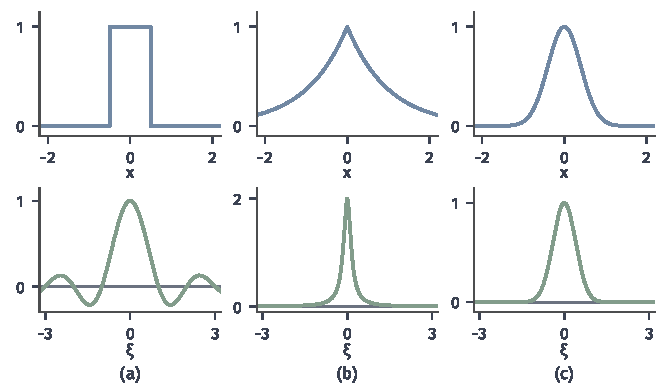
\includegraphics[width=112mm]{figures/04-spaces-measures-and-geometry/03-function-spaces/matplotlib/fourier-three-pairs/figure.pdf}
  \caption{三个Fourier变换对。上排蓝色为原函数，下排绿色为对应的变换。(a)方框$B$与$\sin(\pi\xi)/(\pi\xi)$。(b)双边指数$e^{-\lvert x\rvert}$与$2/(1+4\pi^2\xi^2)$，注意纵轴到$2$。(c)Gauss函数$e^{-\pi x^2}$与它自身。}
  \label{fig:fourier-three-pairs}
\end{BookInlineFigure}

\paragraph{平移、缩放与变换的定义域}

原函数作平移或缩放之后，仍属于$L^1(\mathbb R^d)$，它的变换仍是$\mathbb R^d$上全体频率的函数，变化的只是取值。例如加宽一倍的方框$B(x/2)=\mathbf 1_{[-1,1]}$，直接积分得到
\[
\widehat{B(\cdot/2)}(\xi)=\frac{\sin(2\pi\xi)}{\pi\xi},
\]
它仍定义在整条实轴上，只是零点从非零整数变成了$1/2$的非零整数倍，排得更密。具体的变换规则在第~\ref{sec:fourier-operations}节推导。

这与周期情形不同。改变周期$T$，系数所在的频率集合$\{k/T\}$本身随之改变，相当于换了一组下标。全空间上的Fourier变换没有周期可改，频率集合总是整个$\mathbb R^d$；函数支撑的大小不决定变换的定义域，只影响变换的形状。

\subsection{反演的条件}
\label{sec:fourier-l1-inversion}

变换对每个可积函数都存在，但从$\widehat f$还原$f$是另一个问题。在有限维中，酉矩阵的逆就是共轭转置。这提示最自然的候选：把指数的符号反过来再积分，即对函数$h$定义\term{逆Fourier变换}（inverse Fourier transform）
\begin{equation}
\check h(x)=\int_{\mathbb R^d}h(\xi)e^{2\pi\mathrm ix\cdot\xi}\,\mathrm d\xi .
\label{eq:fourier-inverse}
\end{equation}

如果直接把$\widehat f$的定义代入式~\eqref{eq:fourier-inverse}并交换积分次序，会得到内层积分$\int e^{2\pi\mathrm i(x-y)\cdot\xi}\,\mathrm d\xi$。在矩阵的类比中，这应是单位矩阵的$(x,y)$元，可是这个积分根本不收敛，因为被积函数的模恒为$1$。类比到此失效，反演不能由“$U^*U=I$”直接读出。

方框的例子表明困难是实在的：$\widehat B$不绝对可积，式~\eqref{eq:fourier-inverse}作为Lebesgue积分根本不存在。本小节先在$\widehat f$也可积的条件下建立反演，再讨论更弱条件下的逐点版本。

\paragraph{Gauss核的恒等逼近}

反演的证明不直接处理发散的内层积分，而是在频域乘一个缓慢消失的因子$G(t\xi)$，使一切积分绝对收敛，最后再令$t\to0$。为此引入缩放的Gauss核
\[
G_t(x)=t^{-d}G(x/t),\qquad t>0.
\]
作换元$x=tu$，得到$\int G_t=1$；$t$越小，$G_t$越集中在原点附近。

下面算$G(t\xi)$的逆变换。换元$\eta=t\xi$，再用$G$是偶函数且$\widehat G=G$，得到
\begin{equation}
\int_{\mathbb R^d}G(t\xi)e^{2\pi\mathrm iz\cdot\xi}\,\mathrm d\xi=t^{-d}\,\widehat G(-z/t)=G_t(z).
\label{eq:fourier-gauss-kernel-inverse}
\end{equation}
所以内层那个发散的积分，乘上$G(t\xi)$后就变成了集中在$z=0$附近的$G_t(z)$，这正是“单位矩阵的元”应有的样子。

\begin{lemma}[Gauss核的恒等逼近]
\label{lem:fourier-gauss-approx}
设$f\in L^1(\mathbb R^d)$，$t>0$，记$(f*G_t)(x)=\int f(y)G_t(x-y)\,\mathrm dy$。则
\begin{enumerate}
\item 对每个$x$，
\begin{equation}
\int_{\mathbb R^d}\widehat f(\xi)G(t\xi)e^{2\pi\mathrm ix\cdot\xi}\,\mathrm d\xi=(f*G_t)(x);
\label{eq:fourier-gauss-regularized}
\end{equation}
\item $t\to0$时$\lVert f*G_t-f\rVert_1\to0$。
\end{enumerate}
\end{lemma}

\begin{proof}
第1条。先确认可以交换积分次序：
\[
\int\!\!\int\lvert f(y)\rvert\,G(t\xi)\,\mathrm dy\,\mathrm d\xi=t^{-d}\lVert f\rVert_1<\infty.
\]
于是可以用Fubini定理，再用式~\eqref{eq:fourier-gauss-kernel-inverse}，得到
\[
\begin{aligned}
\int\widehat f(\xi)G(t\xi)e^{2\pi\mathrm ix\cdot\xi}\,\mathrm d\xi
&=\int f(y)\Bigl(\int G(t\xi)e^{2\pi\mathrm i(x-y)\cdot\xi}\,\mathrm d\xi\Bigr)\mathrm dy\\
&=\int f(y)G_t(x-y)\,\mathrm dy.
\end{aligned}
\]

第2条。由$\int G_t=1$，把$f(x)$写进积分，得到
\[
(f*G_t)(x)-f(x)=\int G_t(h)\bigl(f(x-h)-f(x)\bigr)\,\mathrm dh.
\]
取绝对值后对$x$积分，用Tonelli定理交换次序，再换元$h=tu$，记$(\tau_hf)(x)=f(x-h)$，得到
\[
\lVert f*G_t-f\rVert_1\leq\int G_t(h)\lVert\tau_hf-f\rVert_1\,\mathrm dh=\int G(u)\lVert\tau_{tu}f-f\rVert_1\,\mathrm du.
\]
被积函数被$2\lVert f\rVert_1G(u)$控制，且由平移积分连续性逐点趋于零，控制收敛定理给出结论。
\end{proof}

像$G_t$这样非负、积分为$1$、质量随参数集中到原点的核族称为\term{恒等逼近}（approximate identity）：与它卷积几乎不改变函数。第~\ref{chap:smoothing-weak-derivatives}章的磨光核也是恒等逼近，Gauss核的好处是它的Fourier变换可以精确算出。

式~\eqref{eq:fourier-gauss-regularized}的两边分别在频域和空间中描述同一件事，图~\ref{fig:fourier-gauss-smoothing}以方框为例。频域中，$\widehat B$乘上$G(t\xi)$后，高频部分被压掉，积分收敛了；空间中，这对应把方框的跳跃抹平。$t$越小，频域保留的范围越宽，空间中抹平的范围越窄，最终回到原函数。

\begin{BookInlineFigure}
  \centering
  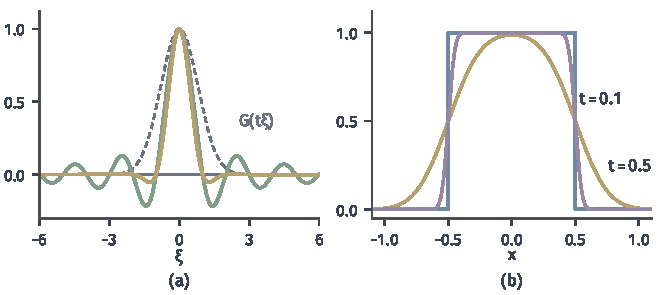
\includegraphics[width=112mm]{figures/04-spaces-measures-and-geometry/03-function-spaces/matplotlib/fourier-gauss-smoothing/figure.pdf}
  \caption{频域乘$G(t\xi)$与空间卷积$G_t$是同一运算，这里$f=B$。(a)绿色为$\widehat B$，灰色虚线为$G(t\xi)$（$t=0.5$），黄色为乘积。(b)蓝色为方框$B$，黄色与紫色为$B*G_t$，$t=0.5$与$t=0.1$；$t$越小，曲线越贴近方框。}
  \label{fig:fourier-gauss-smoothing}
\end{BookInlineFigure}

\paragraph{反演定理}

有了引理，令$t\to0$：左边在$\widehat f$可积时趋于逆变换，右边趋于$f$，反演就得到了。

\begin{theorem}[$L^1$反演定理]
\label{thm:fourier-l1-inversion}
设$f\in L^1(\mathbb R^d)$且$\widehat f\in L^1(\mathbb R^d)$。令
\begin{equation}
g(x)=\int_{\mathbb R^d}\widehat f(\xi)e^{2\pi\mathrm ix\cdot\xi}\,\mathrm d\xi ,
\label{eq:fourier-l1-inversion}
\end{equation}
则$g$是在无穷远处趋于零的连续函数，并且$f=g$几乎处处。若$f$在点$x_0$处连续，则$f(x_0)=g(x_0)$。
\end{theorem}

\begin{proof}
换元$\xi\mapsto-\xi$可知$g$是可积函数$\xi\mapsto\widehat f(-\xi)$的Fourier变换，由定理~\ref{thm:fourier-l1-properties}，它连续且在无穷远处趋于零。

在式~\eqref{eq:fourier-gauss-regularized}中令$t\to0$。左边的被积函数逐点趋于$\widehat f(\xi)e^{2\pi\mathrm ix\cdot\xi}$，并被可积函数$\lvert\widehat f\rvert$控制，所以左边对每个$x$趋于$g(x)$。

另一方面，引理~\ref{lem:fourier-gauss-approx}第2条说明$f*G_t\to f$于$L^1$。按$L^1$收敛的序列有几乎处处收敛的子列（第~\ref{chap:function-normed-spaces}章），所以沿某个子列$t_n\to0$，$(f*G_{t_n})(x)\to f(x)$对几乎每个$x$成立。两个极限相等，故$f=g$几乎处处。

若$f$在$x_0$处连续，对$\varepsilon>0$取$r>0$，使$\lvert x-x_0\rvert<r$时
\[
\lvert f(x)-f(x_0)\rvert<\varepsilon,\qquad\lvert g(x)-g(x_0)\rvert<\varepsilon.
\]
这个球的测度为正，其中有点$x$满足$f(x)=g(x)$，所以$\lvert f(x_0)-g(x_0)\rvert<2\varepsilon$。由$\varepsilon$任意，得到$f(x_0)=g(x_0)$。
\end{proof}

定理有三层含义。第一，反演公式给出的是$f$的一个连续代表，原函数作为等价类与它相等。第二，凡是$\widehat f$可积的$f$，必与一个连续函数几乎处处相等；方框有跳跃，所以$\widehat B$不可积，这与前面的直接计算一致。第三，变换是单射：若$\widehat f=\widehat g$，则$\widehat{f-g}=0$可积，反演给出$f=g$几乎处处，这相当于有限维中“坐标全同则向量相同”。

双边指数满足定理的条件，而且处处连续，所以反演对每个$x$成立：
\[
e^{-\lvert x\rvert}=\int_{\mathbb R}\frac{2}{1+4\pi^2\xi^2}\,e^{2\pi\mathrm ix\xi}\,\mathrm d\xi.
\]
在$x=0$处检验。作换元$u=2\pi\xi$，右边变成
\[
\int_{\mathbb R}\frac{2}{1+4\pi^2\xi^2}\,\mathrm d\xi=\frac1\pi\int_{\mathbb R}\frac{\mathrm du}{1+u^2}=1,
\]
与左边的$e^0=1$一致。

\paragraph{逐点反演与对称截断}

$\widehat f$不可积时，式~\eqref{eq:fourier-inverse}只能理解为某种极限。一维中最常用的是对称截断。对有限的$R$，积分区间有界，Fubini定理可用，内层积分算出来是
\[
\int_{-R}^{R}e^{2\pi\mathrm i(x-y)\xi}\,\mathrm d\xi=\frac{\sin\bigl(2\pi R(x-y)\bigr)}{\pi(x-y)}.
\]
再换元$t=x-y$，得到
\begin{equation}
\int_{-R}^{R}\widehat f(\xi)e^{2\pi\mathrm ix\xi}\,\mathrm d\xi=\int_{\mathbb R}f(x-t)\,\frac{\sin(2\pi Rt)}{\pi t}\,\mathrm dt .
\label{eq:fourier-symmetric-truncation}
\end{equation}
这里的核$\sin(2\pi Rt)/(\pi t)$扮演Dirichlet核的角色。下面需要它的积分，也就是Dirichlet积分
\[
\int_0^\infty\frac{\sin s}{s}\,\mathrm ds=\frac\pi2.
\]

Dirichlet积分可以用周期情形的工具算出。由$\frac1{2\pi}\int_0^\pi D_N=\frac12$和式~\eqref{eq:fourier-dirichlet-closed}，得到
\[
\int_0^\pi\frac{\sin\bigl((N+\tfrac12)t\bigr)}{\sin(t/2)}\,\mathrm dt=\pi.
\]
函数$\frac1{\sin(t/2)}-\frac2t$在$(0,\pi]$上有界（$t\to0$时趋于零），由Riemann--Lebesgue引理，把分母换成$t/2$不改变极限。作换元$s=(N+\tfrac12)t$，于是
\[
\lim_{N\to\infty}\int_0^{(N+1/2)\pi}\frac{\sin s}{s}\,\mathrm ds=\frac\pi2.
\]
反常积分$\int_0^\infty\frac{\sin s}{s}\,\mathrm ds$由分部积分知收敛，极限沿这个子列读出，就是$\pi/2$。

\begin{theorem}[对称截断的逐点反演]
\label{thm:fourier-symmetric-inversion}
设$f\in L^1(\mathbb R)$，并且在每个有界区间上都是分段$C^1$的。则对每个$x$，
\begin{equation}
\lim_{R\to\infty}\int_{-R}^{R}\widehat f(\xi)e^{2\pi\mathrm ix\xi}\,\mathrm d\xi=\frac{f(x+)+f(x-)}2 .
\label{eq:fourier-symmetric-inversion}
\end{equation}
\end{theorem}

\begin{proof}
核$\sin(2\pi Rt)/(\pi t)$是偶函数，所以式~\eqref{eq:fourier-symmetric-truncation}的右边可以写成$(0,\infty)$上的积分，被积函数含$f(x+t)+f(x-t)$。把积分在$t=1$处分开，并在$(0,1)$上减去左右极限，得到三项：
\[
\begin{aligned}
&\int_1^\infty\frac{f(x+t)+f(x-t)}{\pi t}\sin(2\pi Rt)\,\mathrm dt\\
&\quad+\int_0^1\frac{h(t)}{\pi t}\sin(2\pi Rt)\,\mathrm dt\\
&\quad+\bigl(f(x+)+f(x-)\bigr)\int_0^1\frac{\sin(2\pi Rt)}{\pi t}\,\mathrm dt,
\end{aligned}
\]
其中$h(t)=f(x+t)-f(x+)+f(x-t)-f(x-)$。

第一项的被积系数在$(1,\infty)$上可积，因为$f\in L^1$且$1/t\leq1$。第二项的被积系数在$(0,1)$上有界：靠近$t=0$处用定理~\ref{thm:fourier-dirichlet}证明中的单侧Lipschitz估计，其余部分用$f$在有界区间上有界。由引理~\ref{lem:fourier-riemann-lebesgue}，这两项都趋于零。

第三项作换元$s=2\pi Rt$，由Dirichlet积分，得到
\[
\int_0^1\frac{\sin(2\pi Rt)}{\pi t}\,\mathrm dt=\frac1\pi\int_0^{2\pi R}\frac{\sin s}{s}\,\mathrm ds\to\frac12.
\]
\end{proof}

对方框$B$，这一结论在$x=\pm1/2$处给出$1/2$，在其余点给出$B(x)$，这是Dirichlet定理在全空间上的对应结果。

本节的两个问题要分开看待。变换的存在只需要$f\in L^1$，在每个频率处都有确定的值。反演则另需条件：$\widehat f\in L^1$时反演积分绝对收敛，结论在几乎处处意义下成立；只有局部正则性时，要先规定积分的极限方式，结论在每一点成立，跳跃点处得到平均值。

\section{\texorpdfstring{$L^2$}{L2}中的Fourier变换}
\label{sec:fourier-l2}

周期情形的Parseval关系是无限维的勾股定理。全空间上我们也希望有$\int\lvert f\rvert^2=\int\lvert\widehat f\rvert^2$这样的等式，让Fourier变换像酉矩阵一样保持长度。但这个等式属于$L^2$，而上一节的积分定义要求$f\in L^1$。

在$\mathbb R$上两个空间互不包含，反例如下。$s(x)=\sin(\pi x)/(\pi x)$平方可积却不绝对可积，它的不可积性上一节已经算过。另一方面，函数
\[
u(x)=\lvert x\rvert^{-1/2}\mathbf 1_{\{0<\lvert x\rvert<1\}}
\]
绝对可积，$\int u=4$，却不平方可积，因为$\int_{-1}^1\lvert x\rvert^{-1}\,\mathrm dx$发散。

路线与从有理数造实数相同：在交集$L^1\cap L^2$上用原积分定义变换，证明它保持$L^2$范数，再借助稠密性把它延拓到整个$L^2$。在实轴上，$\sqrt2$不能写成有理数，但它是有理数列的极限；一个$L^2$函数也许无法直接积分，但它是$L^1\cap L^2$中函数的极限。

\paragraph{截取逼近}

延拓之前先确认$L^1\cap L^2$在$L^2$中稠密。对$f\in L^2(\mathbb R^d)$，同时截去远处与过大的取值：
\[
f_n=f\,\mathbf 1_{\{\lvert x\rvert\leq n,\ \lvert f(x)\rvert\leq n\}},\qquad n=1,2,\ldots .
\]
$f_n$的支撑含于半径$n$的球中，取值不超过$n$，所以$f_n$可积。又$\lvert f_n\rvert\leq\lvert f\rvert$，所以$f_n\in L^1\cap L^2$。

对几乎每个$x$，$f(x)$有限，当$n\geq\max\{\lvert x\rvert,\lvert f(x)\rvert\}$时$f_n(x)=f(x)$，所以$\lvert f_n-f\rvert^2\to0$几乎处处。又$\lvert f_n-f\rvert^2\leq\lvert f\rvert^2$可积，由控制收敛定理，
\[
\lVert f_n-f\rVert_2\to0.
\]

用一个例子看截断的量。取$g(x)=1/(1+\lvert x\rvert)$，它平方可积（$\int g^2=2$），但$\int g$发散。这时$g\leq1$，只需截去远处，令$g_n=g\mathbf 1_{\{\lvert x\rvert\leq n\}}$，尾部的能量是
\[
\lVert g-g_n\rVert_2^2=2\int_n^\infty\frac{\mathrm dx}{(1+x)^2}=\frac2{1+n}.
\]
$n=1,9,99$时依次为$1$、$0.2$、$0.02$，虽然慢，但趋于零。

同一截取还给出$L^2$中的平移连续性：$y\to0$时$\lVert\tau_yf-f\rVert_2\to0$。论证与引理~\ref{lem:fourier-fejer}的证明相同。$f_n$有界且可积，所以
\[
\lVert\tau_yf_n-f_n\rVert_2^2\leq2n\,\lVert\tau_yf_n-f_n\rVert_1\to0.
\]
而平移保持$L^2$范数，于是
\[
\lVert\tau_yf-f\rVert_2\leq2\lVert f-f_n\rVert_2+\lVert\tau_yf_n-f_n\rVert_2.
\]

\begin{lemma}[$L^2$中的Gauss光滑化]
\label{lem:fourier-gauss-l2}
设$f\in L^2(\mathbb R^d)$，$t>0$。则$f*G_t$对每个$x$有定义，属于$L^2(\mathbb R^d)$，并且$t\to0$时$\lVert f*G_t-f\rVert_2\to0$。若还有$f\in L^1(\mathbb R^d)$，则$f*G_t\in L^1(\mathbb R^d)$且
\begin{equation}
\widehat{f*G_t}(\xi)=\widehat f(\xi)\,G(t\xi).
\label{eq:fourier-gauss-l2-product}
\end{equation}
\end{lemma}

\begin{proof}
由Cauchy--Schwarz不等式，
\[
\int\lvert f(y)\rvert G_t(x-y)\,\mathrm dy\leq\lVert f\rVert_2\lVert G_t\rVert_2,
\]
所以卷积处处有定义。

$G_t(h)\,\mathrm dh$是概率测度，再用一次Cauchy--Schwarz不等式，得到
\[
\lvert(f*G_t)(x)-f(x)\rvert^2\leq\int G_t(h)\lvert f(x-h)-f(x)\rvert^2\,\mathrm dh.
\]
对$x$积分，交换次序，再换元$h=tu$，于是
\[
\lVert f*G_t-f\rVert_2^2\leq\int G(u)\lVert\tau_{tu}f-f\rVert_2^2\,\mathrm du.
\]
被积函数不超过$4\lVert f\rVert_2^2G(u)$，右边有限，所以$f*G_t-f\in L^2$，从而$f*G_t\in L^2$。由平移连续性与控制收敛定理，右边在$t\to0$时趋于零。

若$f\in L^1$，Tonelli定理给出$\lVert f*G_t\rVert_1\leq\lVert f\rVert_1$。再用Fubini定理与换元$z=x-y$，得到
\[
\widehat{f*G_t}(\xi)=\int f(y)e^{-2\pi\mathrm iy\cdot\xi}\Bigl(\int G_t(z)e^{-2\pi\mathrm iz\cdot\xi}\,\mathrm dz\Bigr)\mathrm dy=\widehat f(\xi)\,\widehat{G_t}(\xi).
\]
换元$z=tu$给出$\widehat{G_t}(\xi)=\widehat G(t\xi)=G(t\xi)$。
\end{proof}

式~\eqref{eq:fourier-gauss-l2-product}是第~\ref{sec:fourier-operations}节卷积规则的一个特例，这里要用到它，所以直接验证。

\subsection{等距延拓}
\label{sec:fourier-l2-extension}

\paragraph{交集上的Plancherel恒等式}

先在一个更小的集合上证明能量关系，那里所有积分都绝对收敛。记
\[
D=\{f\in L^1\cap L^2:\widehat f\in L^1\}.
\]
对$f\in D$，$\widehat f$有界且可积，所以也平方可积；由定理~\ref{thm:fourier-l1-inversion}，$f$几乎处处等于$\widehat f$的逆变换。把一个$f$换成反演公式，再交换积分次序，就得到
\[
\begin{aligned}
\int\lvert f\rvert^2\,\mathrm dx
&=\int\overline{f(x)}\Bigl(\int\widehat f(\xi)e^{2\pi\mathrm ix\cdot\xi}\,\mathrm d\xi\Bigr)\mathrm dx\\
&=\int\widehat f(\xi)\,\overline{\int f(x)e^{-2\pi\mathrm ix\cdot\xi}\,\mathrm dx}\,\mathrm d\xi\\
&=\int\lvert\widehat f\rvert^2\,\mathrm d\xi .
\end{aligned}
\]
交换次序的依据是二重积分绝对收敛，其值为$\lVert f\rVert_1\lVert\widehat f\rVert_1<\infty$。

\begin{theorem}[Plancherel恒等式]
\label{thm:fourier-plancherel-l1l2}
若$f\in L^1(\mathbb R^d)\cap L^2(\mathbb R^d)$，则$\widehat f\in L^2(\mathbb R^d)$，并且
\begin{equation}
\lVert\widehat f\rVert_2=\lVert f\rVert_2 .
\label{eq:fourier-plancherel-l1l2}
\end{equation}
\end{theorem}

\begin{proof}
一般的$f$未必属于$D$，用Gauss光滑化把它变成$D$中的元素。令$f_t=f*G_t$。由引理~\ref{lem:fourier-gauss-l2}，$f_t\in L^1\cap L^2$，且$\widehat{f_t}=\widehat f\,G(t\,\cdot)$。$\widehat f$有界、$G(t\,\cdot)$可积，所以$\widehat{f_t}\in L^1$，即$f_t\in D$。

对$f_t$用上面的恒等式，并注意$G(t\xi)^2=e^{-2\pi t^2\lvert\xi\rvert^2}$，得到
\[
\int\lvert\widehat f(\xi)\rvert^2e^{-2\pi t^2\lvert\xi\rvert^2}\,\mathrm d\xi=\lVert f_t\rVert_2^2.
\]
令$t\downarrow0$。左边的被积函数单调增加到$\lvert\widehat f\rvert^2$，由单调收敛定理，左边趋于$\int\lvert\widehat f\rvert^2$。右边由引理~\ref{lem:fourier-gauss-l2}趋于$\lVert f\rVert_2^2$。
\end{proof}

用方框核对。$\lVert B\rVert_2^2=1$，定理说$\int(\sin\pi\xi/(\pi\xi))^2\,\mathrm d\xi=1$。这个积分用初等方法并不好算，下面还会用反演另外验证。

\paragraph{延拓到$L^2$}

现在$f\mapsto\widehat f$是稠密子空间$L^1\cap L^2$到完备空间$L^2$的线性等距映射。第~\ref{chap:metric-space-maps}章证明了：稠密子集上的一致连续映射，若目标空间完备，就有唯一的连续延拓，并且Lipschitz常数保持不变。把它用于这一等距映射，就得到通常所说的\term{Plancherel定理}（Plancherel theorem）。

\begin{theorem}[Plancherel定理]
\label{thm:fourier-plancherel}
存在唯一的连续映射$\mathcal F:L^2(\mathbb R^d)\to L^2(\mathbb R^d)$，使$\mathcal Ff=\widehat f$对$f\in L^1\cap L^2$成立。$\mathcal F$是线性等距：$\lVert\mathcal Ff\rVert_2=\lVert f\rVert_2$。对任意$f\in L^2$，下式在$L^2$范数下成立：
\begin{equation}
\mathcal Ff=\lim_{n\to\infty}\int_{\lvert x\rvert\leq n}f(x)e^{-2\pi\mathrm ix\cdot(\cdot)}\,\mathrm dx .
\label{eq:fourier-plancherel-limit}
\end{equation}
\end{theorem}

\begin{proof}
存在性与唯一性由上述延拓定理给出。

等距性：对$f\in L^2$取$g_n\in L^1\cap L^2$，$g_n\to f$，由$\mathcal F$的连续性与式~\eqref{eq:fourier-plancherel-l1l2}，得到
\[
\lVert\mathcal Ff\rVert_2=\lim_n\lVert\widehat{g_n}\rVert_2=\lim_n\lVert g_n\rVert_2=\lVert f\rVert_2.
\]
线性同样由$L^1\cap L^2$上的线性取极限得到。

最后，$f\mathbf 1_{\{\lvert x\rvert\leq n\}}$在有限测度的球上平方可积，由Cauchy--Schwarz不等式也可积，并在$L^2$中收敛到$f$，所以它们的变换收敛到$\mathcal Ff$。
\end{proof}

此后对$f\in L^2$也写$\widehat f=\mathcal Ff$，称为$f$的Fourier变换；在$L^1\cap L^2$上，这一记号与原积分定义一致。

\paragraph{频域元素是等价类}

延拓得到的$\mathcal Ff$是$L^2$中的元素，即几乎处处相等的函数组成的等价类，不是一个在每个频率处都有确定值的函数。对一般的$f\in L^2$，积分$\int f(x)e^{-2\pi\mathrm ix\cdot\xi}\,\mathrm dx$不必绝对收敛，式~\eqref{eq:fourier-plancherel-limit}的极限也只在范数意义下成立，不保证对某个固定的$\xi$收敛。

例如$s(x)=\sin(\pi x)/(\pi x)$平方可积而不绝对可积，对它不能用定义~\ref{def:fourier-transform-l1}在任何一个频率处读取变换。下一小节将算出$\mathcal Fs=\mathbf 1_{[-1/2,1/2]}$，这是$L^2$中的等式，频率$\pm1/2$处的值没有意义，正如改变方框在端点的取值不改变它所代表的元素。这与$L^1$情形形成对照：那里$\widehat f$是处处有定义的连续函数，可以在单个频率处求值。

\subsection{\texorpdfstring{$L^2$}{L2}反演与Parseval关系}
\label{sec:fourier-l2-inversion}

\paragraph{反演与内积保持}

在$L^2$中，反演有一个干净的形式。记反射$(Rf)(x)=f(-x)$，它是$L^2$上的等距。对$f\in L^1$，直接换元得到
\[
\widehat{Rf}(\xi)=\int f(-x)e^{-2\pi\mathrm ix\cdot\xi}\,\mathrm dx=\widehat f(-\xi).
\]
两边都连续地依赖$f$，所以$\mathcal FR=R\mathcal F$在$L^2$上成立。逆变换式~\eqref{eq:fourier-inverse}恰为$\check h=R\widehat h$，因此它延拓到$L^2$后的映射就是$R\mathcal F$。

\begin{theorem}[$L^2$反演与Parseval关系]
\label{thm:fourier-l2-inversion}
$\mathcal F$是$L^2(\mathbb R^d)$到自身的双射，逆映射为$\mathcal F^{-1}=R\mathcal F$，并且$\mathcal F\mathcal F=R$。对任意$f,g\in L^2(\mathbb R^d)$，
\begin{equation}
\int_{\mathbb R^d}\overline{f(x)}\,g(x)\,\mathrm dx=\int_{\mathbb R^d}\overline{\widehat f(\xi)}\,\widehat g(\xi)\,\mathrm d\xi .
\label{eq:fourier-l2-parseval}
\end{equation}
\end{theorem}

\begin{proof}
先证$R\mathcal F\mathcal F=I$。对$f\in D$，$\widehat f\in L^1\cap L^2$，所以$R\mathcal F(\widehat f)$可以用积分计算，它就是$\widehat f$的逆变换，由定理~\ref{thm:fourier-l1-inversion}等于$f$。所以$R\mathcal F\mathcal F=I$在$D$上成立。

定理~\ref{thm:fourier-plancherel-l1l2}的证明表明，每个$f\in L^1\cap L^2$都是$D$中元素$f*G_t$的$L^2$极限，而$L^1\cap L^2$在$L^2$中稠密，所以$D$在$L^2$中稠密。两边都是连续映射，故$R\mathcal F\mathcal F=I$在$L^2$上成立。

由$R^2=I$得$\mathcal F\mathcal F=R$。再由$\mathcal FR=R\mathcal F$得$\mathcal F(R\mathcal F)=R\mathcal F\mathcal F=I$。所以$\mathcal F$是双射，逆为$R\mathcal F$。

内积保持来自范数保持。对第二个变量线性的复内积，由范数表示的公式是
\[
\langle f,g\rangle=\frac14\sum_{k=0}^3\mathrm i^{-k}\lVert f+\mathrm i^kg\rVert_2^2.
\]
$\mathcal F$线性且保持每个$f+\mathrm i^kg$的范数，所以保持内积。
\end{proof}

这就是有限维酉矩阵的全部性质：保持长度和内积，逆等于“共轭转置”。把$\mathcal F$作用两次等于反射，这一点第~\ref{sec:fourier-discrete}节会用$4\times4$矩阵具体看到。式~\eqref{eq:fourier-l2-parseval}是全空间上的Parseval关系，取$g=f$即能量关系$\lVert\widehat f\rVert_2=\lVert f\rVert_2$，在本章的归一化下两边没有额外常数。

现在可以算出$\mathcal Fs$。方框$B$属于$L^1\cap L^2$，$\widehat B=s$。由$\mathcal F\mathcal F=R$，并注意$B$是偶函数，得到
\[
\mathcal Fs=\mathcal F\mathcal FB=RB=B.
\]
能量关系同时给出
\[
\int_{\mathbb R}\Bigl(\frac{\sin\pi x}{\pi x}\Bigr)^2\,\mathrm dx=\lVert B\rVert_2^2=1.
\]

\paragraph{同一公式的不同含义}

反演公式~\eqref{eq:fourier-l1-inversion}在本章出现了三次，含义各不相同，表~\ref{tab:fourier-inversion-meanings}把它们并列。把积分区域限制在$\lvert\xi\rvert\leq R$得到的截断积分，是否对几乎每个$x$逐点收敛，是深刻得多的问题，本书不讨论。

\begin{BookInlineTable}
  \centering
  \small
  \begin{tabular}{@{}lll@{}}
    \toprule
    条件 & 右边的含义 & 等式的意义\\
    \midrule
    $f,\widehat f\in L^1$ & 绝对收敛的积分 & 几乎处处；连续点处逐点\\
    一维，局部分段$C^1$ & 对称截断的极限 & 每一点；跳跃点取平均\\
    $f\in L^2$ & 截断积分的$L^2$极限 & 范数意义\\
    \bottomrule
  \end{tabular}
  \caption{反演公式在三种条件下的含义。}
  \label{tab:fourier-inversion-meanings}
\end{BookInlineTable}

\paragraph{归一化与常数}

不同文献的Fourier变换只差自变量伸缩与常数因子，但反演与能量公式中的常数必须与定义配套。表~\ref{tab:fourier-normalizations}比较三种常见约定，其中第二、三行用角频率$\omega=2\pi\xi$。

\begin{BookInlineTable}
  \centering
  \small
  \begin{tabularx}{\linewidth}{@{}>{\raggedright\arraybackslash}p{20mm}>{\raggedright\arraybackslash}X>{\raggedright\arraybackslash}p{28mm}@{}}
    \toprule
    约定 & 正变换与反变换 & 能量关系\\
    \midrule
    频率$\xi$（本章） & $\widehat f(\xi)=\int fe^{-2\pi\mathrm ix\cdot\xi}\,\mathrm dx$，$f=\int\widehat fe^{2\pi\mathrm ix\cdot\xi}\,\mathrm d\xi$ & $\int\lvert f\rvert^2=\int\lvert\widehat f\rvert^2$\\
    角频率，正变换不加因子 & $F(\omega)=\int fe^{-\mathrm ix\cdot\omega}\,\mathrm dx$，$f=(2\pi)^{-d}\int Fe^{\mathrm ix\cdot\omega}\,\mathrm d\omega$ & $\int\lvert f\rvert^2=(2\pi)^{-d}\int\lvert F\rvert^2$\\
    角频率，对称归一 & 正、反变换各乘$(2\pi)^{-d/2}$ & $\int\lvert f\rvert^2=\int\lvert F\rvert^2$\\
    \bottomrule
  \end{tabularx}
  \caption{$\mathbb R^d$上Fourier变换的三种常见归一化。各行之间的换算是$F(\omega)=\widehat f(\omega/2\pi)$，对称归一化再乘以$(2\pi)^{-d/2}$；所有结论只差这些常数。}
  \label{tab:fourier-normalizations}
\end{BookInlineTable}

以第二行为例核对常数。作换元$\omega=2\pi\xi$，$\mathrm d\omega=(2\pi)^d\,\mathrm d\xi$，得到
\[
\int\lvert F(\omega)\rvert^2\,\mathrm d\omega=\int\lvert\widehat f(\omega/2\pi)\rvert^2\,\mathrm d\omega=(2\pi)^d\int\lvert\widehat f(\xi)\rvert^2\,\mathrm d\xi,
\]
所以能量关系中出现$(2\pi)^{-d}$。周期情形同样如此：第~\ref{sec:fourier-series}节把$1/(2\pi)$放进内积，Parseval关系才不含常数。

\section{Fourier变换下的运算}
\label{sec:fourier-operations}

有限维中，对称矩阵在特征向量基下变成对角矩阵，矩阵的作用只是把每个坐标乘一个数。平面波$e_\xi(x)=e^{2\pi\mathrm ix\cdot\xi}$对几种基本运算扮演同样的角色。平移$a$之后，
\[
e_\xi(x-a)=e^{-2\pi\mathrm ia\cdot\xi}\,e_\xi(x),
\]
求导之后，
\[
\partial_je_\xi=2\pi\mathrm i\xi_j\,e_\xi .
\]
所以每个平面波都是平移和求导的公共“特征向量”，而特征值是$\xi$的已知函数。这就是频率坐标好用的根本原因：这些运算在频率坐标下都是对角的。

这一说法只是启发。平面波不属于$L^1$，也不属于$L^2$，上面的“特征向量”并不在所讨论的空间里，所以每条规则都要用换元、分部积分或交换积分次序实际证明，而每一步都有前提。本节对每条规则先在$L^1(\mathbb R^d)$中给出证明，再说明它在什么条件下推广到$L^2$，所用的卷积与弱导数来自第~\ref{chap:smoothing-weak-derivatives}章。

\subsection{平移}
\label{sec:fourier-translation}

把函数整体移动$a\in\mathbb R^d$，记$(\tau_af)(x)=f(x-a)$。按上面的特征值，平移不应改变各频率成分的大小，只改变它们的相位。与之对偶的操作是乘以平面波，记$(M_bf)(x)=e^{2\pi\mathrm ib\cdot x}f(x)$，称为\term{调制}（modulation）。

\begin{theorem}[平移与调制]
\label{thm:fourier-translation}
设$f\in L^1(\mathbb R^d)$，$a,b\in\mathbb R^d$。则对每个$\xi$，
\begin{equation}
\widehat{\tau_af}(\xi)=e^{-2\pi\mathrm ia\cdot\xi}\,\widehat f(\xi),\qquad\widehat{M_bf}(\xi)=\widehat f(\xi-b).
\label{eq:fourier-translation}
\end{equation}
两式对$f\in L^2(\mathbb R^d)$在$L^2$意义下同样成立。
\end{theorem}

\begin{proof}
第一式作换元$x=y+a$：
\[
\int f(x-a)e^{-2\pi\mathrm ix\cdot\xi}\,\mathrm dx=\int f(y)e^{-2\pi\mathrm i(y+a)\cdot\xi}\,\mathrm dy=e^{-2\pi\mathrm ia\cdot\xi}\widehat f(\xi).
\]
第二式只需把两个指数合并成$e^{-2\pi\mathrm ix\cdot(\xi-b)}$。

对$L^2$，四个映射$f\mapsto\tau_af$、$f\mapsto M_bf$、乘以$e^{-2\pi\mathrm ia\cdot\xi}$、频率平移$b$都是$L^2$上的等距，$\mathcal F$也是。所以两边作为$f$的映射都连续，又在稠密子空间$L^1\cap L^2$上相等，因而在$L^2$上相等。
\end{proof}

两条规则方向相反，不能混淆。函数平移产生频率上的相位因子，频谱的大小$\lvert\widehat f\rvert$不变，完全看不出平移量；频率平移则来自函数上的相位因子。指数的符号取决于定义中的约定。周期情形有同样的规则，第$k$个坐标乘以$e^{-\mathrm ika}$，证明也是换元。

用$\mathbf 1_{[0,1]}=\tau_{1/2}B$作一个核对。平移规则与式~\eqref{eq:fourier-box}给出
\[
\widehat{\mathbf 1_{[0,1]}}(\xi)=e^{-\pi\mathrm i\xi}\,\frac{\sin\pi\xi}{\pi\xi}.
\]
直接积分得到$\frac{1-e^{-2\pi\mathrm i\xi}}{2\pi\mathrm i\xi}$，提出因子$e^{-\pi\mathrm i\xi}$后，
\[
\frac{1-e^{-2\pi\mathrm i\xi}}{2\pi\mathrm i\xi}=e^{-\pi\mathrm i\xi}\,\frac{e^{\pi\mathrm i\xi}-e^{-\pi\mathrm i\xi}}{2\pi\mathrm i\xi}=e^{-\pi\mathrm i\xi}\,\frac{\sin\pi\xi}{\pi\xi},
\]
两者一致。

\subsection{缩放}
\label{sec:fourier-scaling}

把自变量乘以$\lambda>1$，函数在空间中被压窄。频率的含义是单位长度内的圈数，压窄后同样的振荡出现在更短的长度上，频率应当按$\lambda$放大；同时积分区域缩小，幅度要乘以一个Jacobian因子。下面对一般的可逆线性变换推导这一点。

\begin{theorem}[线性变量替换]
\label{thm:fourier-scaling}
设$f\in L^1(\mathbb R^d)$，$\bm A$是$d\times d$可逆实矩阵。则
\begin{equation}
\widehat{f\circ\bm A}(\xi)=\frac1{\lvert\det\bm A\rvert}\,\widehat f\bigl(\bm A^{-\top}\xi\bigr).
\label{eq:fourier-linear-change}
\end{equation}
特别地，对实数$\lambda\neq0$，
\begin{equation}
\widehat{f(\lambda\,\cdot)}(\xi)=\lvert\lambda\rvert^{-d}\,\widehat f(\xi/\lambda).
\label{eq:fourier-scaling}
\end{equation}
\end{theorem}

\begin{proof}
作换元$y=\bm Ax$。Lebesgue测度在线性变换下乘以$\lvert\det\bm A\rvert$，即$\mathrm dx=\lvert\det\bm A\rvert^{-1}\mathrm dy$（第~\ref{chap:integration}章）。指数中的内积变成
\[
x\cdot\xi=(\bm A^{-1}y)\cdot\xi=y\cdot(\bm A^{-\top}\xi).
\]
代入定义，于是
\[
\int f(\bm Ax)e^{-2\pi\mathrm ix\cdot\xi}\,\mathrm dx=\frac1{\lvert\det\bm A\rvert}\int f(y)e^{-2\pi\mathrm iy\cdot\bm A^{-\top}\xi}\,\mathrm dy.
\]
取$\bm A=\lambda\bm I$，$\det\bm A=\lambda^d$，$\bm A^{-\top}\xi=\xi/\lambda$，就是第二式。
\end{proof}

公式中三个量各有来源。频率尺度$\xi/\lambda$说明：$\lambda>1$时原函数压窄，变换展宽。因子$\lvert\lambda\rvert^{-d}$是Jacobian，它随维数$d$改变；各坐标分别按$\lambda_1,\ldots,\lambda_d$缩放时，因子为$\prod_i\lvert\lambda_i\rvert^{-1}$，第$i$个频率坐标变为$\xi_i/\lambda_i$。转置逆$\bm A^{-\top}$说明频率按对偶方式变换：旋转在频域中仍是同一个旋转，剪切则不然。

图~\ref{fig:fourier-scaling}取$\lambda=1/2$。方框加宽一倍，式~\eqref{eq:fourier-scaling}给出
\[
\widehat{B(\cdot/2)}(\xi)=2\,\widehat B(2\xi)=\frac{\sin(2\pi\xi)}{\pi\xi},
\]
与上一节的直接计算一致。空间中变宽，频域中变窄；中央的高度翻倍，因为$\xi=0$处的值就是函数的积分，$\int B(x/2)\,\mathrm dx=2$。

\begin{BookInlineFigure}
  \centering
  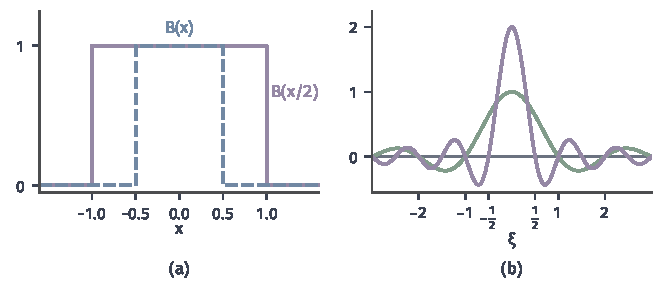
\includegraphics[width=112mm]{figures/04-spaces-measures-and-geometry/03-function-spaces/matplotlib/fourier-scaling/figure.pdf}
  \caption{缩放的对偶。(a)蓝色虚线为方框$B(x)$，紫色为加宽一倍的$B(x/2)$。(b)绿色为$\widehat B$，第一个零点在$\xi=\pm1$；紫色为$B(x/2)$的变换，第一个零点在$\xi=\pm\frac12$，中央高度为$2$。}
  \label{fig:fourier-scaling}
\end{BookInlineFigure}

Gauss核也可以检验。$G_t=t^{-d}G(\cdot/t)$对应$\lambda=1/t$，公式给出
\[
\widehat{G_t}(\xi)=t^{-d}\cdot t^d\,\widehat G(t\xi)=G(t\xi),
\]
正是反演证明中用到的等式。

在$L^2$中常用保持范数的伸缩
\[
D_\lambda f=\lvert\lambda\rvert^{d/2}f(\lambda\,\cdot).
\]
式~\eqref{eq:fourier-scaling}给出$\widehat{D_\lambda f}=D_{1/\lambda}\widehat f$。两边都是$L^2$上的等距，在$L^1\cap L^2$上相等，所以在$L^2$上相等。这一归一化把Jacobian因子平分到两侧，第~\ref{chap:wavelet-transform}章的小波伸缩采用同样的写法。

\subsection{微分}
\label{sec:fourier-differentiation}

周期情形的分部积分给出$\widehat{f'}(k)=\mathrm ik\widehat f(k)$，边界项因周期性抵消。全空间上没有周期，边界项能否消失取决于函数在远处的行为；在函数不可导的点，还要借助弱导数。下面先处理边界项自动消失的情形，再处理一般情形。

\paragraph{光滑紧支撑函数}

设$f$连续可微且支撑紧。固定其余坐标，在一个包含支撑的有界区间上对$x_j$分部积分，边界项为零，得到
\[
\int\partial_jf(x)\,e^{-2\pi\mathrm ix\cdot\xi}\,\mathrm dx_j=-\int f(x)\,\partial_j\bigl(e^{-2\pi\mathrm ix\cdot\xi}\bigr)\,\mathrm dx_j.
\]
指数对$x_j$求导带下来因子$-2\pi\mathrm i\xi_j$，所以
\[
\int\partial_jf(x)\,e^{-2\pi\mathrm ix\cdot\xi}\,\mathrm dx_j=2\pi\mathrm i\xi_j\int f(x)e^{-2\pi\mathrm ix\cdot\xi}\,\mathrm dx_j.
\]
再对其余坐标积分（Fubini定理），得到
\[
\widehat{\partial_jf}(\xi)=2\pi\mathrm i\xi_j\,\widehat f(\xi).
\]
求导在频域中变成乘以$2\pi\mathrm i\xi_j$，与开头的特征值一致。

\paragraph{弱导数可积的情形}

一般的可积函数没有紧支撑，也未必处处可导。第~\ref{chap:smoothing-weak-derivatives}章用测试恒等式定义了弱导数：若局部可积函数$g$对所有$\varphi\in C_c^\infty(\mathbb R^d)$满足$\int f\,\partial_j\varphi=-\int g\,\varphi$，就称$g$为$f$的弱导数$\partial_jf$。要把这个恒等式用于$e^{-2\pi\mathrm ix\cdot\xi}$，需要先把它截断成紧支撑函数，再让截断半径趋于无穷，并控制截断边缘产生的项。

\begin{theorem}[微分规则]
\label{thm:fourier-derivative}
设$f\in L^1(\mathbb R^d)$，且$f$关于$x_j$的弱导数$\partial_jf$存在并属于$L^1(\mathbb R^d)$。则对每个$\xi\in\mathbb R^d$，
\begin{equation}
\widehat{\partial_jf}(\xi)=2\pi\mathrm i\xi_j\,\widehat f(\xi).
\label{eq:fourier-derivative}
\end{equation}
\end{theorem}

\begin{proof}
取光滑函数$\chi$，满足$0\leq\chi\leq1$，在$\lvert x\rvert\leq1$上等于$1$，在$\lvert x\rvert\geq2$上等于$0$；这样的截断函数由第~\ref{chap:smoothing-weak-derivatives}章的磨光构造得到。对$R>0$令
\[
\varphi_R(x)=\chi(x/R)\,e^{-2\pi\mathrm ix\cdot\xi},
\]
它的实部与虚部都是测试函数，所以测试恒等式对$\varphi_R$成立。按乘积求导，
\[
\partial_j\varphi_R(x)=\Bigl[\frac1R(\partial_j\chi)(x/R)-2\pi\mathrm i\xi_j\chi(x/R)\Bigr]e^{-2\pi\mathrm ix\cdot\xi}.
\]
代入测试恒等式，得到
\[
\begin{aligned}
\int\partial_jf(x)\chi(x/R)e^{-2\pi\mathrm ix\cdot\xi}\,\mathrm dx
={}&-\frac1R\int f(x)(\partial_j\chi)(x/R)e^{-2\pi\mathrm ix\cdot\xi}\,\mathrm dx\\
&+2\pi\mathrm i\xi_j\int f(x)\chi(x/R)e^{-2\pi\mathrm ix\cdot\xi}\,\mathrm dx .
\end{aligned}
\]
令$R\to\infty$。左边与右边第二项的被积函数分别被$\lvert\partial_jf\rvert$与$\lvert f\rvert$控制，且$\chi(x/R)\to1$，由控制收敛定理，它们分别趋于$\widehat{\partial_jf}(\xi)$与$2\pi\mathrm i\xi_j\widehat f(\xi)$。右边第一项是截断边缘的贡献，其模不超过
\[
\frac1R\sup\lvert\partial_j\chi\rvert\,\lVert f\rVert_1\to0.
\]
\end{proof}

证明中$f\in L^1$承担了控制边缘项的任务：截断函数的导数只有$1/R$大小，乘上可积的$f$后整体趋于零。这里没有要求$f$在远处逐点趋于零。

\paragraph{光滑性与衰减}

微分规则把光滑性转换为高频衰减。由定理~\ref{thm:fourier-l1-properties}，
\[
2\pi\lvert\xi_j\rvert\,\lvert\widehat f(\xi)\rvert=\lvert\widehat{\partial_jf}(\xi)\rvert\leq\lVert\partial_jf\rVert_1 .
\]
若各阶弱导数$\partial^\alpha f$（$\lvert\alpha\rvert\leq m$）都可积，逐次使用规则，得到
\[
\widehat{\partial^\alpha f}(\xi)=(2\pi\mathrm i\xi)^\alpha\,\widehat f(\xi),\qquad
(2\pi\mathrm i\xi)^\alpha=\prod_j(2\pi\mathrm i\xi_j)^{\alpha_j},
\]
所以$\lvert\widehat f(\xi)\rvert$按$\lvert\xi\rvert^{-m}$衰减。

对偶地，原函数在远处衰减得快，变换就光滑。若$f$与$x_jf$都可积，在积分号下对$\xi_j$求导（被积函数的导数被$2\pi\lvert x_jf\rvert$控制），得到
\[
\partial_{\xi_j}\widehat f=\widehat{-2\pi\mathrm ix_jf}.
\]

用双边指数核对。$f(x)=e^{-\lvert x\rvert}$在$0$处不可导，但有可积的弱导数$-\operatorname{sgn}(x)e^{-\lvert x\rvert}$。把弱导数的变换分成两段积分，得到
\[
-\frac1{1+2\pi\mathrm i\xi}+\frac1{1-2\pi\mathrm i\xi}=\frac{4\pi\mathrm i\xi}{1+4\pi^2\xi^2}.
\]
由式~\eqref{eq:fourier-double-exponential}，这恰好等于$2\pi\mathrm i\xi\,\widehat f(\xi)$，与定理一致。

方框$B$不满足定理的条件。形式地计算，
\[
2\pi\mathrm i\xi\,\widehat B(\xi)=2\mathrm i\sin(\pi\xi)=e^{\pi\mathrm i\xi}-e^{-\pi\mathrm i\xi}.
\]
它不随$\lvert\xi\rvert\to\infty$趋于零，由Riemann--Lebesgue引理不可能是可积函数的变换。它对应的是在$x=-1/2$与$x=1/2$处的两个符号相反的点质量，这正是跳跃函数的导数不能由局部可积函数表示的情形，超出了本节$L^1$的框架。

$L^2$函数的弱导数有对应的频域刻画：$f$与$\partial_jf$都属于$L^2$时，式~\eqref{eq:fourier-derivative}在$L^2$意义下成立。它是第~\ref{chap:sobolev-spaces}章用频率权刻画Sobolev空间的出发点，证明也留到那里。

\subsection{卷积}
\label{sec:fourier-convolution}

第~\ref{chap:smoothing-weak-derivatives}章对$f,g\in L^1(\mathbb R^d)$定义了卷积$(f*g)(x)=\int f(x-y)g(y)\,\mathrm dy$，证明它几乎处处有定义，并且
\[
\lVert f*g\rVert_1\leq\lVert f\rVert_1\lVert g\rVert_1.
\]

卷积是平移的加权叠加：
\[
f*g=\int g(y)\,\tau_yf\,\mathrm dy.
\]
平移在频域中是乘以相位因子，叠加之后应当得到$\widehat f$乘以$g$的相位加权和，也就是$\widehat f\,\widehat g$。在有限维的类比中，这说明卷积算子也在频率坐标下对角，第$\xi$个对角元就是$\widehat g(\xi)$。

\begin{theorem}[卷积规则]
\label{thm:fourier-convolution}
若$f,g\in L^1(\mathbb R^d)$，则对每个$\xi$，
\begin{equation}
\widehat{f*g}(\xi)=\widehat f(\xi)\,\widehat g(\xi).
\label{eq:fourier-convolution}
\end{equation}
\end{theorem}

\begin{proof}
先确认可以交换积分次序：
\[
\int\!\!\int\lvert f(x-y)\rvert\,\lvert g(y)\rvert\,\mathrm dx\,\mathrm dy=\lVert f\rVert_1\lVert g\rVert_1<\infty.
\]
由Fubini定理交换次序，再对内层换元$z=x-y$，得到
\[
\begin{aligned}
\widehat{f*g}(\xi)&=\int g(y)\Bigl(\int f(x-y)e^{-2\pi\mathrm ix\cdot\xi}\,\mathrm dx\Bigr)\mathrm dy\\
&=\int g(y)e^{-2\pi\mathrm iy\cdot\xi}\,\mathrm dy\cdot\int f(z)e^{-2\pi\mathrm iz\cdot\xi}\,\mathrm dz .
\end{aligned}
\]
\end{proof}

方框与自身的卷积是三角形。$(B*B)(x)$等于区间$[-1/2,1/2]$与$[x-1/2,x+1/2]$的重叠长度，所以
\[
(B*B)(x)=\Lambda(x)=\max\{0,1-\lvert x\rvert\}.
\]
图~\ref{fig:fourier-convolution-triangle}(a)画的是$x=0.4$的情形，重叠长度为$0.6$，正是(b)中$\Lambda(0.4)$的值。

卷积规则给出$\Lambda$的变换：
\[
\widehat\Lambda(\xi)=\Bigl(\frac{\sin\pi\xi}{\pi\xi}\Bigr)^2.
\]
它按$\xi^{-2}$衰减，是可积的，而$\Lambda$连续，所以由定理~\ref{thm:fourier-l1-inversion}，反演在每一点成立。在$x=0$处读出
\[
\int_{\mathbb R}\Bigl(\frac{\sin\pi\xi}{\pi\xi}\Bigr)^2\,\mathrm d\xi=\Lambda(0)=1,
\]
与上一节由能量关系算出的值一致。卷积使跳跃变成尖点，频域中的衰减也从$\xi^{-1}$加快到$\xi^{-2}$，图~\ref{fig:fourier-convolution-triangle}(c)中实线的旁瓣明显更小。

\begin{BookInlineFigure}
  \centering
  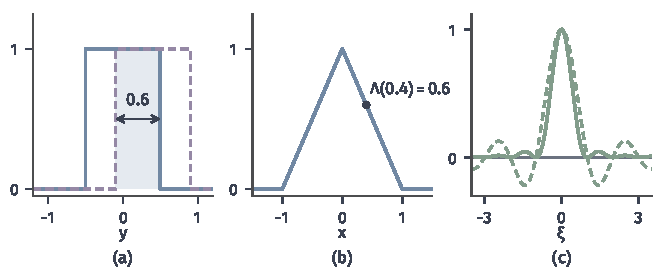
\includegraphics[width=112mm]{figures/04-spaces-measures-and-geometry/03-function-spaces/matplotlib/fourier-convolution-triangle/figure.pdf}
  \caption{方框的自卷积。(a)蓝色为$B(y)$，紫色虚线为$B(x-y)$（$x=0.4$），浅蓝色区域为重叠部分，长度$0.6$。(b)$\Lambda=B*B$，黑点对应(a)的$x$。(c)绿色虚线为$\widehat B$，绿色实线为$\widehat\Lambda=\widehat B^{\,2}$。}
  \label{fig:fourier-convolution-triangle}
\end{BookInlineFigure}

\paragraph{推广到$L^2$}

推广时要分别确认输入在哪个空间、卷积落在哪个空间、等式在什么意义下成立。

第一种情形是$f\in L^1$、$g\in L^2$。由Cauchy--Schwarz不等式，
\[
\lvert(f*g)(x)\rvert^2\leq\int\lvert f(x-y)\rvert\,\mathrm dy\cdot\int\lvert f(x-y)\rvert\,\lvert g(y)\rvert^2\,\mathrm dy.
\]
对$x$积分，得到
\[
\lVert f*g\rVert_2\leq\lVert f\rVert_1\lVert g\rVert_2,
\]
所以卷积落在$L^2$中，并且连续地依赖$g$。

此时等式$\widehat{f*g}=\widehat f\,\widehat g$在$L^2$中成立。当$g\in L^1\cap L^2$时它由定理~\ref{thm:fourier-convolution}给出。左边是$g$的连续映射，右边是乘以有界函数$\widehat f$，也连续。两边在稠密子空间上相等，所以在整个$L^2$上相等。

第二种情形是$f,g\in L^2$。此时$(f*g)(x)$对每个$x$都有定义，模不超过$\lVert f\rVert_2\lVert g\rVert_2$，由$L^2$平移连续性它还是连续函数；但它一般不属于$L^1$，也不必属于$L^2$。另一方面，$\widehat f\widehat g$作为两个$L^2$函数的乘积是可积的。因此正确的对应是逆变换，而不是$L^2$中的变换等式：
\begin{equation}
(f*g)(x)=\int_{\mathbb R^d}\widehat f(\xi)\,\widehat g(\xi)\,e^{2\pi\mathrm ix\cdot\xi}\,\mathrm d\xi\qquad\text{对每个}\ x .
\label{eq:fourier-l2-convolution}
\end{equation}

证明用Parseval关系。令$h_x(y)=f(x-y)$，则
\[
(f*g)(x)=\int h_x\,g=\langle\overline{h_x},g\rangle.
\]
由平移、反射规则，
\[
\widehat{h_x}(\xi)=e^{-2\pi\mathrm ix\cdot\xi}\widehat f(-\xi).
\]
再由共轭的规则
\[
\widehat{\overline u}(\xi)=\overline{\widehat u(-\xi)}
\]
（对$L^1$函数直接验证，再延拓到$L^2$），得到
\[
\widehat{\overline{h_x}}(\xi)=\overline{e^{2\pi\mathrm ix\cdot\xi}\widehat f(\xi)}.
\]
代入式~\eqref{eq:fourier-l2-parseval}，共轭抵消，即得式~\eqref{eq:fourier-l2-convolution}。

例如$f=g=s$时，$\widehat f\widehat g=B\cdot B=B$，式~\eqref{eq:fourier-l2-convolution}给出$s*s=s$，它平方可积却不可积。

这三种情形研究的都是Fourier变换怎样把卷积这一运算转为乘法。把卷积看作对信号的作用，讨论哪些频率被保留、哪些被削弱，属于滤波问题，在\BookChapterRef{chap:signal-systems}{卷九“信号系统”章}研究。

\section{Fourier表示与离散变换}
\label{sec:fourier-discrete}

到目前为止出现了两种频率表示：周期函数的Fourier系数是整数下标的序列，全空间函数的Fourier变换是连续频率的函数。实际计算中还有第三种：有限个数组成的向量，用有限个频率表示。三者都用复指数作坐标，但输入对象、频率集合和成立的意义都不同。本节先把三种对象并列，再说明从一种转到另一种时，需要哪些额外的约定，以及每种约定改变了什么。

\paragraph{离散Fourier变换}

有限向量的情形最简单。设$N\geq1$，把$\bm x\in\mathbb C^N$的分量记为$x[0],\ldots,x[N-1]$，并把下标看作模$N$的整数，即首尾相接。此时允许的频率只有$N$个，对应的复指数为$e^{2\pi\mathrm ikn/N}$，$k=0,\ldots,N-1$。

\begin{definition}[离散Fourier变换]
\label{def:fourier-dft}
$\bm x\in\mathbb C^N$的\term{离散Fourier变换}（discrete Fourier transform, DFT）为
\[
\widehat x[k]=\sum_{n=0}^{N-1}x[n]e^{-2\pi\mathrm ikn/N},\qquad k=0,\ldots,N-1 .
\]
\end{definition}

逆变换与能量关系都来自单位根的正交性：对整数$m$，$\sum_{n=0}^{N-1}e^{2\pi\mathrm imn/N}$在$N\mid m$时等于$N$，否则是公比$q=e^{2\pi\mathrm im/N}\neq1$且$q^N=1$的几何级数，等于$(1-q^N)/(1-q)=0$。由此
\[
x[n]=\frac1N\sum_{k=0}^{N-1}\widehat x[k]e^{2\pi\mathrm ikn/N},\qquad
\sum_{n=0}^{N-1}\lvert x[n]\rvert^2=\frac1N\sum_{k=0}^{N-1}\lvert\widehat x[k]\rvert^2 .
\]
这里所有的和都是有限和，不存在收敛问题，变换是$\mathbb C^N$上的可逆线性映射，$N^{-1/2}$倍的变换矩阵是酉矩阵。常数$1/N$的位置同样是约定，与第~\ref{sec:fourier-l2}节的表格同理。

\paragraph{三种表示的对象}

下表把三种表示并列。它们的差别首先在输入：全空间上的函数、一个周期上的函数、$N$个数。输入不同，频率集合与成立的意义也随之不同。

\begin{table}[!htb]
  \centering
  \caption{三种Fourier表示的输入对象、频率集合与成立意义。表中周期情形写成一般周期$T$，第~\ref{sec:fourier-series}节取$T=2\pi$。}
  \label{tab:fourier-three-representations}
  \small
  \begin{tabularx}{\linewidth}{@{}l>{\raggedright\arraybackslash}X>{\raggedright\arraybackslash}X>{\raggedright\arraybackslash}X@{}}
    \toprule
    表示 & 输入对象 & 频率集合 & 成立的意义\\
    \midrule
    Fourier变换 & $\mathbb R^d$上的$L^1$或$L^2$函数 & $\xi\in\mathbb R^d$ & $L^1$：处处有值；$L^2$：等价类\\
    Fourier级数 & 周期$T$的$L^1$或$L^2$函数 & $k/T$，$k\in\mathbb Z$ & $L^2$展开；逐点另需条件\\
    离散变换 & $\mathbb C^N$中的向量 & $k$，$k=0,\ldots,N-1$（模$N$） & 有限和，精确可逆\\
    \bottomrule
  \end{tabularx}
\end{table}

这三种对象不能直接互相代替。一个全空间函数没有周期，不能直接取Fourier系数；一个周期函数有无穷多个系数，不能直接作$N$点变换；$N$个数不是函数，没有连续频率。从一种表示转到另一种，必须先把对象本身转过去，下面三个操作各完成一种转换。

\paragraph{周期化：从全空间到周期}

把全空间函数变成周期函数的自然做法是把所有平移叠加起来。对$f\in L^1(\mathbb R)$，定义它的\term{周期化}（periodization）
\[
(Pf)(x)=\sum_{n\in\mathbb Z}f(x+n).
\]
由Tonelli定理，$\int_0^1\sum_n\lvert f(x+n)\rvert\,\mathrm dx=\int_{\mathbb R}\lvert f\rvert<\infty$，所以级数对几乎每个$x$绝对收敛，$Pf$以$1$为周期且在一个周期上可积。

\begin{theorem}[周期化的系数]
\label{thm:fourier-periodization}
若$f\in L^1(\mathbb R)$，则$Pf$按周期$1$计算的Fourier系数为
\[
\int_0^1(Pf)(x)e^{-2\pi\mathrm ikx}\,\mathrm dx=\widehat f(k),\qquad k\in\mathbb Z .
\]
\end{theorem}

\begin{proof}
上面的绝对收敛估计允许交换求和与积分。$e^{-2\pi\mathrm ikx}$以$1$为周期，所以
\begin{equation*}
\begin{aligned}
\int_0^1\sum_nf(x+n)e^{-2\pi\mathrm ikx}\,\mathrm dx&=\sum_n\int_n^{n+1}f(y)e^{-2\pi\mathrm iky}\,\mathrm dy\\
&=\int_{\mathbb R}f(y)e^{-2\pi\mathrm iky}\,\mathrm dy .
\end{aligned}
\end{equation*}
\end{proof}

定理说明，周期化后的Fourier系数恰是原变换在整数频率上的取值，连续频率被取样成了离散频率。代价在原函数一侧：$Pf$把相距整数的各段叠在一起。若$f$支撑在长度不超过$1$的区间内，各段不重叠，$Pf$在一个周期上就是$f$，没有信息损失；否则不同位置的值混在一起，由$Pf$不能还原$f$。以$f=e^{-\lvert x\rvert}$为例，$Pf$的系数为$2/(1+4\pi^2k^2)$，而$Pf$本身在每一点都叠加了无穷多个平移。由这一系数等式还可以得到逐点的Poisson求和公式$\sum_nf(n)=\sum_k\widehat f(k)$，但那需要额外的正则性，这里不展开。

\paragraph{取样：从周期函数到有限向量}

把周期函数变成$N$个数的自然做法是在一个周期内等距取样。设$g$以$1$为周期，Fourier系数$\widehat g(m)=\int_0^1g(x)e^{-2\pi\mathrm imx}\,\mathrm dx$绝对可和；由定理~\ref{thm:fourier-uniform}（换成周期$1$），二次连续可微就足够。此时Fourier级数一致收敛到$g$，在每一点成立。取样$x[n]=g(n/N)$，$n=0,\ldots,N-1$。

\begin{theorem}[取样的离散变换]
\label{thm:fourier-sampling-aliasing}
在上述条件下，
\[
\widehat x[k]=N\sum_{j\in\mathbb Z}\widehat g(k+jN),\qquad k=0,\ldots,N-1 .
\]
\end{theorem}

\begin{proof}
$x[n]=\sum_m\widehat g(m)e^{2\pi\mathrm imn/N}$，级数绝对收敛，可以与关于$n$的有限和交换：
\[
\widehat x[k]=\sum_m\widehat g(m)\sum_{n=0}^{N-1}e^{2\pi\mathrm i(m-k)n/N}=N\sum_{m\equiv k\ (\mathrm{mod}\ N)}\widehat g(m),
\]
最后一步用了单位根的正交性。
\end{proof}

于是$\widehat x[k]/N$不是单个系数$\widehat g(k)$，而是所有与$k$模$N$同余的频率的系数之和：取样后，频率$k$与$k\pm N,k\pm2N,\ldots$无法区分。这一现象称为\term{混叠}（aliasing）。例如$g(x)=\cos(6\pi x)$只有$\widehat g(\pm3)=1/2$，取$N=4$时，$m=3$落在$k=3$，$m=-3\equiv1$落在$k=1$，样本的离散变换在$k=1,3$处等于$2$，与$\cos(2\pi x)$的样本完全相同；事实上$\cos(3\pi n/2)=\cos(\pi n/2)$对每个整数$n$成立。反过来，若$g$是三角多项式，且非零系数的频率$m$都满足$\lvert m\rvert<N/2$，则每个同余类中至多有一个非零系数，离散变换精确给出全部系数。

\paragraph{截断：从全空间到有限记录}

实际只能观察全空间函数的一段。把$f$截断到长度$L$的区间上，相当于乘以方框$B_L=\mathbf 1_{[-L/2,L/2]}$。乘积在频域中对应卷积：对$f,g\in L^2$，把第~\ref{sec:fourier-convolution}节$L^2$卷积的对应关系用于$\widehat f,\widehat g$，再用$\mathcal F\mathcal F=R$，可得$\widehat{fg}=\widehat f*\widehat g$。所以截断后的变换是$\widehat f$与$\widehat{B_L}(\xi)=\sin(\pi L\xi)/(\pi\xi)$的卷积，原来集中在某个频率的成分会向邻近频率扩散。

由此可以看清把连续变换交给有限计算的完整链条：先截断（频域中与$\widehat{B_L}$卷积），再以$L$为周期周期化（频率被取样到$k/L$），最后在一个周期内取$N$个样本（频率模$N/L$混叠）。每一步都引入一种约定，也带来一种相应的误差，离散变换给出的数只在这些约定下近似连续变换。这些误差何时可以忽略、怎样控制，取决于原函数的衰减与光滑性，后者正是第~\ref{sec:fourier-operations}节的微分规则所描述的。

本节只核对三种表示的对象和它们之间的精确关系。把这些表示用于具体信号，比较信号的频谱，属于\BookChapterRef{chap:signal-analysis}{卷九“信号的表示与比较”章}；卷积作为系统对信号的作用以及滤波，属于\BookChapterRef{chap:signal-systems}{卷九“信号系统”章}；由样本恢复信号的条件与方法，属于\BookChapterRef{chap:sampling-signal-recovery}{卷九“采样与信号恢复”章}。

\section{本章小结}
\label{sec:fourier-summary}

本章开头问：用复指数为函数换上频率坐标，对哪些函数有意义，在什么意义下能还原，运算规则在什么条件下成立。

周期函数的回答是Fourier级数。复指数$e^{\mathrm ikx}$在归一化内积下标准正交，Fejér核的非负平均证明了它们完备，于是每个$L^2$周期函数都有范数收敛的展开，Parseval关系是无限维的勾股定理。这一展开描述的是几乎处处等价类，逐点与一致收敛要另加条件：分段$C^1$函数的级数在每点收敛到左右极限的平均，$C^2$函数的系数按$k^{-2}$衰减，级数一致收敛；跳跃函数的部分和不可能一致收敛，跳跃附近出现约$9\%$的Gibbs超调。

全空间上的函数没有周期，下标连成了$\mathbb R^d$，而平面波不再属于所讨论的空间，类比开始失效，每一步都要直接证明。对$L^1$函数，Fourier变换在每个频率处都有确定值，是有界、连续、在无穷远处趋于零的函数。变换的存在与反演是两个问题：$\widehat f$也可积时，借助Gauss核的恒等逼近，反演积分给出$f$的连续代表，与$f$几乎处处相等；方框这样的跳跃函数变换不可积，只能在局部正则条件下用对称截断逐点反演，跳跃点处仍得到平均值。

能量关系属于$L^2$。截取说明$L^1\cap L^2$在$L^2$中稠密，Plancherel恒等式先在交集上成立，再由稠密延拓把变换唯一地推广为$L^2$上的等距。所得的变换是双射，满足$\mathcal F\mathcal F=R$，保持内积，性质与酉矩阵相同，但频域元素只是等价类，不能一律在单个频率处求值。同一个反演公式，在三种情形下分别表示绝对收敛积分的几乎处处等式、对称截断的逐点极限与$L^2$范数极限。

运算规则说明频率坐标使若干算子对角化。平移只改相位，调制平移频率；线性变量替换$\bm A$使频率按$\bm A^{-\top}$变换并带来因子$\lvert\det\bm A\rvert^{-1}$；弱导数可积时，求导变成乘以$2\pi\mathrm i\xi_j$，光滑性因而对应高频衰减；卷积在$L^1$中变成逐点乘积，推广到$L^1\times L^2$与$L^2\times L^2$时，输出所在的空间与等式的意义都要重新核对。

离散Fourier变换是真正的有限维酉变换（差一个归一化常数）。连续频率、周期系数与离散变换之间的转换分别需要周期化、取样与截断，它们带来重叠、混叠与频率扩散。

Fourier表示用整体振荡的频率组织函数，每个坐标都依赖整个定义域上的值，局部的跳跃会影响所有高频坐标。第~\ref{chap:wavelet-transform}章改用尺度与位置同时组织局部细节；有限项截断与频带截断的逼近误差，以及系数衰减怎样转化为误差的速度，在第~\ref{chap:function-approximation}章统一研究。


\chapter{小波变换}
\label{chap:wavelet-transform}

第~\ref{chap:functions-as-vectors}章把函数看成一条无限长的向量$[\ldots,f(x),\ldots]$，它的每个分量只报告一个点上的取值。第~\ref{chap:fourier-transform}章换到三角函数基，每个坐标报告一个频率的强度，却要用整个周期上的积分才能读出。这两种坐标各走一个极端：前者只知道位置，后者只知道频率。

一段记录大部分时间平稳，只在少数位置突然跳变，这样的函数放在频率坐标里并不省事，因为一处跳变会让所有频率的系数都不为零。我们希望有一组基，它的坐标同时带着尺度和位置两个标号：先记录整体水平，再逐层记录“这一块的左半和右半相差多少”。这样，平稳区域的细节接近零，一处跳变在每一层只影响覆盖它的少数几块。

小波系数就是这样的坐标：函数这条无限维向量，换到一组多尺度标准正交基之后读出的分量。本章的问题是这组基怎样造出来，它在什么意义下能重构原函数，以及定义域有边界时要做什么调整。

全章从能手算的情形开始。第~\ref{sec:wavelet-finite-haar}节对$2^J$个取值反复求平均与半差，把这个过程整理成$\mathbb R^{2^J}$中的一次正交换基。第~\ref{sec:wavelet-scaling-detail}节把这些取值放回区间$[0,1]$上的分段常数函数，说明每一步换了哪组基函数。第~\ref{sec:wavelet-interval-expansion}节让层数趋于无穷，证明这组基在$L^2([0,1])$中完备。

后三节把构造推广出去。第~\ref{sec:wavelet-real-line}节在全实轴上建立一般的正交多分辨率结构，并讨论比Haar更光滑、能抵消更多多项式的小波。第~\ref{sec:wavelet-boundary}节处理基函数跨过区间端点的问题。第~\ref{sec:wavelet-fourier-comparison}节在同一个周期区间上比较Fourier坐标和小波坐标。

本章使用第~\ref{chap:function-inner-product-spaces}章的正交投影与正交展开，以及第~\ref{chap:fourier-transform}章的Fourier级数。截断误差随项数怎样变化的定量结论在第~\ref{chap:function-approximation}章研究，用小波系数刻画函数正则性的Besov范数在第~\ref{chap:besov-spaces}章建立。

\section{有限Haar变换}
\label{sec:wavelet-finite-haar}

取非负整数$J$，把区间$[0,1)$等分成$N=2^J$段，每段记录一个数，得到向量$\bm a=(a_0,\ldots,a_{N-1})$。这是第~\ref{chap:functions-as-vectors}章函数向量最简单的情形：输入只有$N$个，函数就是$\mathbb R^N$中的一个点。

我们想把这$N$个数改写成两类信息：整体有多高，以及各处在不同尺度上怎样起伏；并且改写以后还能原样拼回去。本节全部在$\mathbb R^N$中计算。

\subsection{逐层平均与差值}
\label{sec:wavelet-average-difference}

\paragraph{一对数的平均与半差}
从两个数开始。相邻取值$a,b$可以换成它们的平均与半差：
\begin{equation}
 s=\frac{a+b}{2},\qquad d=\frac{a-b}{2}.
 \label{eq:wavelet-average-difference}
\end{equation}
$s$记录这两个数共同的水平，$d$记录它们相对平均各偏离多少。

反过来，把两式相加、相减，就得到
\[
 a=s+d,\qquad b=s-d.
\]
所以这一步没有丢失信息，只是换了记法。若$a=b$，则$d=0$：没有起伏的地方，差值就是零。

\paragraph{逐层分解}
对长度$N=2^J$的向量，先把分量两两分组，得到$N/2$个平均和$N/2$个半差。半差保存下来，平均组成一个长度减半的新向量，再对它重复同一步。做完$J$步后只剩一个数，即全部取值的平均。

保存下来的半差个数是
\[
 \frac N2+\frac N4+\cdots+1=N-1,
\]
连同总平均恰好$N$个数，与原向量的分量一样多。恢复时按相反次序进行：从总平均和最粗一层的半差算出两个平均，再与下一层的半差配合得到四个平均，直到恢复全部$N$个取值。每一步都只用加减，所以整个分解是可逆的线性变换。

\begin{example}[四个取值的平均与半差]
\label{ex:wavelet-four-values-average}
取$\bm a=(2,4,8,6)$。第一步把相邻两对分别换成平均和半差：
\[
 (2,4)\mapsto(3,-1),\qquad(8,6)\mapsto(7,1).
\]
第二步对两个平均$(3,7)$再做一次：
\[
 (3,7)\mapsto(5,-2).
\]
于是原向量被记为总平均$5$、两半之间的半差$-2$，以及细层半差$-1,1$。

恢复时先由总平均和粗层半差得到两半的平均：
\[
 5+(-2)=3,\qquad 5-(-2)=7.
\]
再由细层半差得到原来的四个取值：
\[
 3+(-1)=2,\quad3-(-1)=4,\quad7+1=8,\quad7-1=6.
\]
\end{example}

图~\ref{fig:wavelet-average-tree}把这个例子画成了一棵树。沿树向下，每一层的绿框只把平均继续往下传，黄框则留在原地不再变动，这就是逐层分解“只继续处理平均”的含义。

\begin{BookInlineFigure}
  \centering
  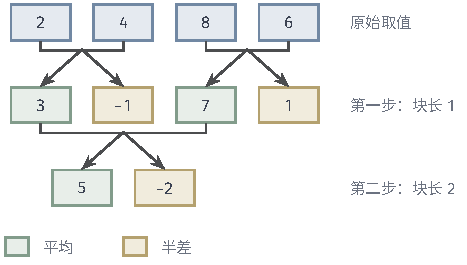
\includegraphics[width=79.07mm]{figures/04-spaces-measures-and-geometry/03-function-spaces/tikz/wavelet-average-tree/figure.pdf}
  \caption{对$(2,4,8,6)$的逐层平均与半差。蓝框是原始取值，绿框是平均，黄框是半差。每一步把一对框换成一个平均和一个半差，半差不再变动，平均进入下一步。}
  \label{fig:wavelet-average-tree}
\end{BookInlineFigure}

\paragraph{差值记录的尺度与位置}
每个半差都对应一个“块”和这一块的左右两半。细层的$-1$只比较$a_0$与$a_1$，块长为一段；粗层的$-2$比较前两段的平均$3$与后两段的平均$7$，块长为两段。块的长短给出尺度，块的位置给出位置，块越短，半差描述的变化越局部。

局部性可以直接检验。把$a_2$从$8$改成$9$，得到$(2,4,9,6)$。第一步的半差和平均变成
\[
 (2,4)\mapsto(3,-1),\qquad(9,6)\mapsto\Bigl(\frac{15}2,\frac32\Bigr).
\]
第二步对平均$(3,15/2)$再做一次，得到
\[
 \Bigl(3,\frac{15}2\Bigr)\mapsto\Bigl(\frac{21}4,-\frac94\Bigr).
\]
比较前后两组数，比较$a_0$与$a_1$的半差$-1$不变，变化的只有包含第$2$段的那些块：细层的$1$变成$3/2$，粗层的$-2$变成$-9/4$，总平均$5$变成$21/4$。一处取值的改动在每一层只影响一个系数。

\subsection{正交变换与逆变换}
\label{sec:wavelet-orthogonal-transform}

上一小节的新坐标已经能够恢复原向量，但还不是一组标准正交基下的坐标，因为它没有保持平方和。由式~\eqref{eq:wavelet-average-difference}直接计算，
\[
 s^2+d^2=\frac{(a+b)^2+(a-b)^2}{4}=\frac{a^2+b^2}{2}.
\]
每做一步，平方和减半。第~\ref{chap:function-inner-product-spaces}章的正交展开要求坐标平方和等于长度的平方，所以我们把两个新系数都乘以$\sqrt2$。

\paragraph{二阶正交变换}
把一对取值$(a,b)$换成
\begin{equation}
 \begin{bmatrix}s\\d\end{bmatrix}
 =\bm H_2\begin{bmatrix}a\\b\end{bmatrix},\qquad
 \bm H_2=\frac{1}{\sqrt2}\begin{bmatrix}1&1\\1&-1\end{bmatrix}.
 \label{eq:wavelet-h2}
\end{equation}
即$s=(a+b)/\sqrt2$，$d=(a-b)/\sqrt2$。这里沿用记号$s,d$，它们比式~\eqref{eq:wavelet-average-difference}中的量都大$\sqrt2$倍。

直接相乘可以核对
\[
 \bm H_2^{\top}\bm H_2=\frac12\begin{bmatrix}2&0\\0&2\end{bmatrix}=\bm I.
\]
所以$\bm H_2$是正交矩阵，这一步保持平方和，逆矩阵等于转置。$\bm H_2$还是对称的，于是逆变换与正变换形式相同。正交矩阵的这些性质见\BookChapterRef{chap:inner-product-spaces}{卷二第4章“内积空间”}。

\paragraph{多层变换}
对长度$N=2^J$的向量，第一层对全部$N/2$对取值作用$\bm H_2$，得到$N/2$个粗系数和$N/2$个细节系数。第二层只对粗系数两两作用$\bm H_2$，细节系数原样保留；依此类推，共做$J$层。

每一层在被处理的坐标上是若干个$\bm H_2$拼成的分块对角正交矩阵，在其余坐标上是恒等，所以每一层都是正交变换，它们的复合也是正交变换。我们把输出排成“最粗项在前，细节由粗到细”：先写最后剩下的一个粗系数，再写最粗一层的细节，最后写第一层得到的$N/2$个细节。

记这样得到的矩阵为$\bm W_N$，称$\bm c=\bm W_N\bm a$为$\bm a$的\term{Haar变换}（Haar transform）。由正交性，
\begin{equation}
 \lVert\bm c\rVert_2=\lVert\bm a\rVert_2,\qquad \bm a=\bm W_N^{\top}\bm c.
 \label{eq:wavelet-finite-haar-isometry}
\end{equation}
计算量也很小：第一层处理$N/2$对，第二层$N/4$对，总共$N-1$对。每对只做两次加减和两次乘以$1/\sqrt2$，所以运算次数与$N$成正比。

\begin{example}[四个取值的正交Haar变换]
\label{ex:wavelet-four-values-orthogonal}
仍取$\bm a=(2,4,8,6)$。第一层把两对取值分别作用$\bm H_2$：
\[
 (2,4)\mapsto(3\sqrt2,-\sqrt2),\qquad(8,6)\mapsto(7\sqrt2,\sqrt2).
\]
第二层把粗系数$(3\sqrt2,7\sqrt2)$再作用一次：
\[
 (3\sqrt2,7\sqrt2)\mapsto\Bigl(\frac{10\sqrt2}{\sqrt2},\frac{-4\sqrt2}{\sqrt2}\Bigr)=(10,-4).
\]
按约定排序，得到
\[
 \bm c=(10,-4,-\sqrt2,\sqrt2).
\]

这四个数也可以一次写成矩阵乘法：
\[
 \bm W_4=\begin{bmatrix}
 1/2&1/2&1/2&1/2\\
 1/2&1/2&-1/2&-1/2\\
 1/\sqrt2&-1/\sqrt2&0&0\\
 0&0&1/\sqrt2&-1/\sqrt2
 \end{bmatrix}.
\]
各行长度为$1$且两两正交。平方和核对如下：
\[
 4+16+64+36=120,\qquad 100+16+2+2=120.
\]

逆变换$\bm W_4^{\top}\bm c$逐分量计算，四个分量依次是
\[
 5-2-1=2,\quad5-2+1=4,\quad5+2+1=8,\quad5+2-1=6.
\]
这恢复了原向量。
\end{example}

\paragraph{矩阵的各行就是新基}
$\bm c=\bm W_4\bm a$的第$i$个分量是$\bm W_4$第$i$行与$\bm a$的点积。所以$\bm W_4$的四行组成$\mathbb R^4$的一组新标准正交基，而$\bm c$是$\bm a$在这组基下的坐标。

第一行是常数向量，读取整体水平；第二行把前后两半相减，读取最粗的起伏；后两行只在相邻两个位置非零，读取最细的局部起伏。从标准基换到这组基，向量本身没有变，变的只是读取它的方式。

\paragraph{与平均和半差的关系}
比较两个例子，对应系数之间的比例是
\[
 10=2\times5,\quad-4=2\times(-2),\quad-\sqrt2=\sqrt2\times(-1),\quad\sqrt2=\sqrt2\times1.
\]
一般地，若一个系数对应由$2^m$个原始取值组成的块，则正交变换给出的系数等于$2^{m/2}$乘以该块的平均或半差。

对$m$归纳可以验证这一点。两个长为$2^{m-1}$的子块，平均记为$s_L,s_R$，归纳假设说它们的粗系数是$2^{(m-1)/2}s_L$和$2^{(m-1)/2}s_R$。再作用$\bm H_2$，第一个分量是
\[
 \frac{2^{(m-1)/2}(s_L+s_R)}{\sqrt2}=2^{m/2}\cdot\frac{s_L+s_R}{2},
\]
这正是$2^{m/2}$乘以大块的平均，半差同理。两种算法携带相同的信息，区别只在每个系数的比例因子，正交版本用这些因子换来了长度不变。

\section{尺度空间与细节空间}
\label{sec:wavelet-scaling-detail}

上一节的$2^J$个取值可以看成一个函数：在区间$[0,1)$的第$k$段上取常值$a_k$。这样，平均与差值就变成了对函数的运算，Haar变换就变成了在同一个函数空间中更换基函数。本节先建立由分段常数函数组成的尺度空间，再用正交补定义细节空间，最后核对取值向量与函数坐标之间相差的归一化因子。全节在$L^2([0,1])$中讨论，内积为$\langle f,g\rangle=\int_0^1\overline{f(x)}g(x)\,dx$，按第~\ref{chap:inner-product-spaces}章的约定对第一个变量共轭线性；本章出现的基函数都是实值的。

\subsection{尺度空间}
\label{sec:wavelet-scaling-spaces}

对整数$j\geq0$和$0\leq k<2^j$，记
\[
I_{j,k}=\bigl[k2^{-j},(k+1)2^{-j}\bigr),
\]
称为第$j$层的\term{二进区间}（dyadic interval）。第$j$层的$2^j$个二进区间互不相交，并起来是$[0,1)$。尺度$j$决定区间长度$2^{-j}$，位置$k$决定区间落在哪里。端点$x=1$只是一个零测集，在$L^2([0,1])$中不影响任何元素，所以下面不再区分$[0,1)$与$[0,1]$。

\begin{definition}[Haar尺度空间]
\label{def:wavelet-scaling-space}
对整数$j\geq0$，令$V_j$为$L^2([0,1])$中在每个$I_{j,k}$上几乎处处取常值的元素组成的子空间，称为第$j$层的\term{尺度空间}（scaling space）。令
\[
\varphi_{j,k}=2^{j/2}\mathbf{1}_{I_{j,k}}\qquad(0\leq k<2^j).
\]
\end{definition}

因子$2^{j/2}$的作用是归一化。不同的$\varphi_{j,k}$支撑在不相交的区间上，内积为零；而$\lVert\varphi_{j,k}\rVert_2^2=2^j\cdot2^{-j}=1$。$V_j$中的每个元素都是$\sum_kb_k\mathbf{1}_{I_{j,k}}$的形式，所以$\{\varphi_{j,k}\}_{0\leq k<2^j}$是$V_j$的标准正交基，$\dim V_j=2^j$。有限维子空间是闭的，第~\ref{chap:inner-product-spaces}章的正交投影可以直接使用。

\paragraph{嵌套}
每个第$j$层区间恰好是两个第$j+1$层区间的并：$I_{j,k}=I_{j+1,2k}\cup I_{j+1,2k+1}$。在$I_{j,k}$上取常值的函数，在这两个子区间上当然也取常值，所以
\[
V_0\subset V_1\subset V_2\subset\cdots .
\]
层级越高，允许的分段越细，空间越大。$V_0$只含常数函数。

\paragraph{投影就是取区间平均}
$L^2([0,1])$中的函数在有限测度区间上可积（由Cauchy--Schwarz不等式，$\int_I|f|\leq\lvert I\rvert^{1/2}\lVert f\rVert_2$），所以每个区间上的平均有意义。设$P_j$是到$V_j$的正交投影。用标准正交基写出，
\begin{equation}
P_jf=\sum_{k=0}^{2^j-1}\langle\varphi_{j,k},f\rangle\varphi_{j,k}
=\sum_{k=0}^{2^j-1}\Bigl(2^j\int_{I_{j,k}}f(x)\,dx\Bigr)\mathbf{1}_{I_{j,k}} .
\label{eq:wavelet-projection-average}
\end{equation}
括号中的数正是$f$在$I_{j,k}$上的平均。所以$P_jf$在每个第$j$层区间上取$f$在该区间的平均值，它是$V_j$中离$f$最近的函数。例如$f(x)=x$时，$P_0f\equiv1/2$，$P_1f$在$[0,1/2)$上为$1/4$、在$[1/2,1)$上为$3/4$。

\subsection{细节空间}
\label{sec:wavelet-detail-spaces}

从$V_j$到$V_{j+1}$，空间多出了$2^{j+1}-2^j=2^j$维。多出来的部分应当恰好记录“每个第$j$层区间的左右两半有何不同”，因为在第$j$层这一差别被平均掉了。用正交补把这部分单独取出。

\begin{definition}[Haar细节空间与Haar函数]
\label{def:wavelet-detail-space}
对整数$j\geq0$，令$W_j=V_{j+1}\cap V_j^{\perp}$，称为第$j$层的\term{细节空间}（detail space）。令
\[
\psi=\mathbf{1}_{[0,1/2)}-\mathbf{1}_{[1/2,1)},\qquad
\psi_{j,k}=2^{j/2}\bigl(\mathbf{1}_{I_{j+1,2k}}-\mathbf{1}_{I_{j+1,2k+1}}\bigr)\qquad(0\leq k<2^j),
\]
称$\psi_{j,k}$为\term{Haar函数}（Haar function）。
\end{definition}

$\psi_{j,k}$在$I_{j,k}$的左半取$2^{j/2}$、右半取$-2^{j/2}$，在其余位置为零。用变量代换可以写成$\psi_{j,k}(x)=2^{j/2}\psi(2^jx-k)$，所以全部Haar函数都由同一个$\psi$平移、缩放而来。

\begin{theorem}[细节空间的标准正交基]
\label{thm:wavelet-detail-basis}
对每个$j\geq0$，$\{\psi_{j,k}\}_{0\leq k<2^j}$是$W_j$的标准正交基，并且$V_{j+1}=V_j\oplus W_j$，两者正交。
\end{theorem}

\begin{proof}
$\psi_{j,k}$在每个第$j+1$层区间上取常值，属于$V_{j+1}$。它与$\varphi_{j,k'}$正交：$k'\neq k$时支撑不交；$k'=k$时
\[
\langle\varphi_{j,k},\psi_{j,k}\rangle=2^{j}\bigl(2^{-j-1}-2^{-j-1}\bigr)=0 .
\]
所以$\psi_{j,k}\in V_j^{\perp}$，从而$\psi_{j,k}\in W_j$。不同的$\psi_{j,k}$支撑不交，且$\lVert\psi_{j,k}\rVert_2^2=2^j\cdot2^{-j}=1$，它们是标准正交的。

有限维空间$V_{j+1}$中，闭子空间$V_j$的正交补$W_j$满足$V_{j+1}=V_j\oplus W_j$，维数为$2^{j+1}-2^j=2^j$。$W_j$中有$2^j$个标准正交向量，它们线性无关，因而构成$W_j$的基。
\end{proof}

也可以直接看出$V_{j+1}$中的每个函数都能用两组基表示：由定义，
\[
\mathbf{1}_{I_{j+1,2k}}=\frac{2^{-j/2}}{2}\bigl(\varphi_{j,k}+\psi_{j,k}\bigr),\qquad
\mathbf{1}_{I_{j+1,2k+1}}=\frac{2^{-j/2}}{2}\bigl(\varphi_{j,k}-\psi_{j,k}\bigr).
\]
这两个式子正是平均与半差的函数版本：一个细区间上的指示函数，等于所在粗区间的平均部分加上或减去一个细节。

\paragraph{逐层分解}
把定理~\ref{thm:wavelet-detail-basis}反复用于$V_J,V_{J-1},\ldots,V_1$，得到正交直和分解
\begin{equation}
V_J=V_0\oplus W_0\oplus W_1\oplus\cdots\oplus W_{J-1}.
\label{eq:wavelet-finite-decomposition}
\end{equation}
维数核对为$1+1+2+\cdots+2^{J-1}=2^J$。相应地，$\{\varphi_{0,0}\}\cup\{\psi_{j,k}:0\leq j<J,\ 0\leq k<2^j\}$是$V_J$的另一组标准正交基。

用投影写出，到$W_j$的正交投影是$P_{j+1}-P_j$。所以第$j$层细节就是“用第$j+1$层区间平均表示”与“用第$j$层区间平均表示”之差，正是较粗表示中缺少的局部差异。仍以$f(x)=x$为例，$P_1f-P_0f$在左半为$-1/4$、右半为$1/4$。另一方面$\langle\psi_{0,0},f\rangle=\int_0^{1/2}x\,dx-\int_{1/2}^1x\,dx=1/8-3/8=-1/4$，于是$\langle\psi_{0,0},f\rangle\psi_{0,0}$在两半上分别为$-1/4$和$1/4$，两种算法一致。

\subsection{值向量与函数坐标}
\label{sec:wavelet-values-coordinates}

现在把第~\ref{sec:wavelet-finite-haar}节的有限计算准确地放进$V_J$。设$f=\sum_{k=0}^{N-1}a_k\mathbf{1}_{I_{J,k}}$，$N=2^J$，即$f$在第$k$段上取值$a_k$。它的平方积分是
\[
\lVert f\rVert_2^2=\sum_{k=0}^{N-1}a_k^2\cdot2^{-J},
\]
与取值向量的欧氏平方和差一个因子$2^{-J}$。原因是每段的长度为$2^{-J}$。改用标准正交基表示，$f=\sum_k(2^{-J/2}a_k)\varphi_{J,k}$，所以$f$在基$\{\varphi_{J,k}\}$下的坐标是$2^{-J/2}\bm a$。这个坐标向量的欧氏长度才等于$\lVert f\rVert_2$。

\paragraph{一步变换就是一次换基}
在相邻两个细区间上，由定义有
\[
\varphi_{j,k}=\frac{\varphi_{j+1,2k}+\varphi_{j+1,2k+1}}{\sqrt2},\qquad
\psi_{j,k}=\frac{\varphi_{j+1,2k}-\varphi_{j+1,2k+1}}{\sqrt2}.
\]
若$f$在这两个细区间上的部分是$c_0\varphi_{j+1,2k}+c_1\varphi_{j+1,2k+1}$，代入上式验证可得
\[
c_0\varphi_{j+1,2k}+c_1\varphi_{j+1,2k+1}
=\frac{c_0+c_1}{\sqrt2}\varphi_{j,k}+\frac{c_0-c_1}{\sqrt2}\psi_{j,k}.
\]
右端的两个系数正是式~\eqref{eq:wavelet-h2}中$\bm H_2$作用在$(c_0,c_1)$上的结果。所以对坐标向量$2^{-J/2}\bm a$作有限Haar变换，得到的正是$f$在基$\{\varphi_{0,0}\}\cup\{\psi_{j,k}\}$下的坐标，排序与第~\ref{sec:wavelet-orthogonal-transform}小节的约定一致：先是$\langle\varphi_{0,0},f\rangle$，再是由粗到细的$\langle\psi_{j,k},f\rangle$。

\begin{example}[四段函数的Haar系数]
\label{ex:wavelet-four-values-function}
取$J=2$，$f$在四段上依次取$2,4,8,6$。坐标向量是$2^{-1}\bm a=(1,2,4,3)$。第一层得$(3/\sqrt2,-1/\sqrt2)$与$(7/\sqrt2,1/\sqrt2)$，第二层把$(3/\sqrt2,7/\sqrt2)$换成$(5,-2)$，所以
\[
\bigl(\langle\varphi_{0,0},f\rangle,\langle\psi_{0,0},f\rangle,\langle\psi_{1,0},f\rangle,\langle\psi_{1,1},f\rangle\bigr)=\Bigl(5,-2,-\frac{1}{\sqrt2},\frac{1}{\sqrt2}\Bigr).
\]
这些数也可以直接积分核对。$\langle\varphi_{0,0},f\rangle=\int_0^1f=(2+4+8+6)/4=5$是$f$的平均；$\langle\psi_{0,0},f\rangle=(2+4)/4-(8+6)/4=-2$；$\langle\psi_{1,0},f\rangle=\sqrt2(2/4-4/4)=-1/\sqrt2$；$\langle\psi_{1,1},f\rangle=\sqrt2(8/4-6/4)=1/\sqrt2$。

它们与例~\ref{ex:wavelet-four-values-orthogonal}的欧氏系数$(10,-4,-\sqrt2,\sqrt2)$逐项相差因子$2^{-J/2}=1/2$。能量核对为$\lVert f\rVert_2^2=(4+16+64+36)/4=30$与$25+4+1/2+1/2=30$。此时保持的是函数的平方积分，而不是取值向量的平方和。
\end{example}

这个归一化在实际计算中容易混淆：直接对取值向量作正交Haar变换，得到的数要再乘以$2^{-J/2}$才是$L^2$中的系数。若只关心系数的相对大小，因子无关紧要；若要用系数估计函数的$L^2$误差，就必须带上它。

\section{区间上的Haar展开}
\label{sec:wavelet-interval-expansion}

有限层级的空间$V_J$只含在第$J$层二进区间上取常值的函数。$f(x)=x$这样简单的函数也不在任何$V_J$中，因为它在每个区间内都在变化。要用Haar函数表示一般的$L^2([0,1])$函数，必须让层级无限增加，并说明这样做确实能逼近任意元素。本节先证明尺度空间的并是稠密的，再用第~\ref{chap:inner-product-spaces}章的正交展开得到系数、重构与能量等式。

\subsection{尺度空间的稠密性}
\label{sec:wavelet-scaling-density}

我们要证明：任给$f\in L^2([0,1])$和$\varepsilon>0$，存在某个$j$和$g\in V_j$，使$\lVert f-g\rVert_2<\varepsilon$。$V_j$中的元素称为二进阶梯函数。思路是把一般函数逐步化简：先截去大值，再换成简单函数，再换成有限个区间的指示函数，最后把区间端点移到二进点上。每一步的误差都可以任意小。

\begin{theorem}[二进阶梯函数的稠密性]
\label{thm:wavelet-dyadic-dense}
$\bigcup_{j\geq0}V_j$在$L^2([0,1])$中稠密。因此对每个$f\in L^2([0,1])$，
\[
\lVert f-P_jf\rVert_2\to0\qquad(j\to\infty),
\]
并且$\lVert f-P_jf\rVert_2$随$j$单调不增。
\end{theorem}

\begin{proof}
\emph{第一步：截去大值。}对$M>0$，令$f_M=f\mathbf{1}_{\{\lvert f\rvert\leq M\}}$。逐点有$f_M\to f$（$M\to\infty$），且$\lvert f-f_M\rvert^2\leq\lvert f\rvert^2$可积。由控制收敛定理，$\lVert f-f_M\rVert_2\to0$。所以只需逼近有界可测函数。

\emph{第二步：换成简单函数。}由第~\ref{chap:measure}章的简单函数逼近，有界可测函数$f_M$（复值时分别处理实部与虚部）可以被只取有限个值的简单函数一致逼近。区间$[0,1]$的测度为$1$，一致误差不超过$\delta$时，$L^2$误差也不超过$\delta$。所以只需逼近简单函数，又由线性只需逼近单个指示函数$\mathbf{1}_E$，$E\subset[0,1]$可测。

\emph{第三步：换成有限个区间。}由第~\ref{chap:smoothing-weak-derivatives}章所用的Lebesgue测度的开集外逼近，对$\delta>0$存在开集$U\supset E$，$\lambda(U\setminus E)<\delta$。实轴上的开集是可数个互不相交开区间的并，$U=\bigcup_iJ_i$，且$\sum_i\lambda(J_i)=\lambda(U)<\infty$；取足够多项使剩余部分的测度小于$\delta$，记前$n$个区间之并为$G$。于是$\lambda(E\mathbin{\triangle}G)\leq\lambda(U\setminus E)+\lambda(U\setminus G)<2\delta$。把$G$换成$G\cap[0,1]$不增大对称差，因为$E\subset[0,1]$。指示函数之差只取$0,\pm1$，所以$\lVert\mathbf{1}_E-\mathbf{1}_{G\cap[0,1]}\rVert_2^2=\lambda(E\mathbin{\triangle}(G\cap[0,1]))<2\delta$。

\emph{第四步：端点移到二进点。}对区间$[a,b]\subset[0,1]$，把$a$、$b$分别换成不超过它们的最大的$2^{-j}$整数倍$a_j$、$b_j$。$[a_j,b_j)$是若干个第$j$层二进区间之并，其指示函数属于$V_j$，并且$\lambda([a,b]\mathbin{\triangle}[a_j,b_j))\leq\lvert a-a_j\rvert+\lvert b-b_j\rvert\leq2^{1-j}$，所以$L^2$误差不超过$2^{(1-j)/2}$。有限个区间的指示函数之和，可以对足够大的同一个$j$同时这样处理。四步合起来，任意$f$都能被某个$V_j$中的函数以任意精度逼近。

\emph{收敛与单调性。}给定$\varepsilon>0$，取$j_1$和$g\in V_{j_1}$使$\lVert f-g\rVert_2<\varepsilon$。对$j\geq j_1$，$g\in V_{j_1}\subset V_j$，而$P_jf$是$V_j$中离$f$最近的元素，故$\lVert f-P_jf\rVert_2\leq\lVert f-g\rVert_2<\varepsilon$。同样由$V_j\subset V_{j+1}$得$\lVert f-P_{j+1}f\rVert_2\leq\lVert f-P_jf\rVert_2$。
\end{proof}

证明的最后一段只用到两件事：空间是嵌套的，投影给出最佳逼近。所以“并稠密”自动转化为“投影列收敛”，不需要对每个$f$单独估计$P_jf$。

\begin{example}[线性函数的投影误差]
\label{ex:wavelet-linear-projection-error}
取$f(x)=x$。在每个第$j$层区间上，$P_jf$等于区间中点$m$，记$h=2^{-j}$为区间长度，则
\[
\lVert f-P_jf\rVert_2^2=\sum_{k=0}^{2^j-1}\int_{I_{j,k}}(x-m)^2\,dx=2^j\cdot\frac{h^3}{12}=\frac{4^{-j}}{12},
\]
即$\lVert f-P_jf\rVert_2=2^{-j}/(2\sqrt3)$。层级每增加一层，误差减半。定理~\ref{thm:wavelet-dyadic-dense}只保证误差趋于零，并不给出这样的速度；速度来自$f$本身的光滑性，一般理论见第~\ref{chap:function-approximation}章。
\end{example}

\subsection{系数与重构}
\label{sec:wavelet-coefficients-reconstruction}

稠密性把有限层的分解~\eqref{eq:wavelet-finite-decomposition}推广到整个$L^2([0,1])$。为了与后面实轴上的情形对照，起始层不必是第$0$层：固定整数$j_0\geq0$，由定理~\ref{thm:wavelet-detail-basis}反复分解，对$J>j_0$有$V_J=V_{j_0}\oplus W_{j_0}\oplus\cdots\oplus W_{J-1}$。

\begin{theorem}[区间上的Haar展开]
\label{thm:wavelet-haar-expansion}
固定整数$j_0\geq0$。函数族
\[
\{\varphi_{j_0,k}:0\leq k<2^{j_0}\}\cup\{\psi_{j,k}:j\geq j_0,\ 0\leq k<2^j\}
\]
是$L^2([0,1])$的标准正交基。对每个$f\in L^2([0,1])$，在$L^2$范数下
\begin{equation}
f=\sum_{k=0}^{2^{j_0}-1}\langle\varphi_{j_0,k},f\rangle\varphi_{j_0,k}+\sum_{j=j_0}^{\infty}\sum_{k=0}^{2^j-1}\langle\psi_{j,k},f\rangle\psi_{j,k},
\label{eq:wavelet-haar-expansion}
\end{equation}
并且
\begin{equation}
\lVert f\rVert_2^2=\sum_{k=0}^{2^{j_0}-1}\lvert\langle\varphi_{j_0,k},f\rangle\rvert^2+\sum_{j=j_0}^{\infty}\sum_{k=0}^{2^j-1}\lvert\langle\psi_{j,k},f\rangle\rvert^2 .
\label{eq:wavelet-haar-parseval}
\end{equation}
把$j$求和截到$j\leq J-1$所得的部分和等于$P_Jf$。
\end{theorem}

\begin{proof}
不同层的细节空间$W_j$彼此正交，并都与$V_{j_0}$正交：若$j<j'$，则$W_j\subset V_{j+1}\subset V_{j'}$，而$W_{j'}\perp V_{j'}$。同一层内的正交性由定理~\ref{thm:wavelet-detail-basis}给出，所以整个函数族是标准正交的。它的有限线性组合包含每个$V_J$（$J\geq j_0$），由定理~\ref{thm:wavelet-dyadic-dense}在$L^2([0,1])$中稠密，所以它是完备的标准正交系。展开式与Parseval等式由第~\ref{chap:inner-product-spaces}章的正交展开得到。截到$j\leq J-1$的部分和是$f$在$V_{j_0}\oplus W_{j_0}\oplus\cdots\oplus W_{J-1}=V_J$上的正交投影，即$P_Jf$。
\end{proof}

每一层只有有限个系数，所以式~\eqref{eq:wavelet-haar-expansion}的外层是对$j$的级数，内层是有限和，不存在同层内求和次序的问题。按第~\ref{chap:inner-product-spaces}章的结论，标准正交展开的收敛也不依赖项的排列。

\paragraph{粗项不能省略}
每个Haar函数在$[0,1]$上的积分都是零。若去掉式~\eqref{eq:wavelet-haar-expansion}中的粗项，剩下的级数只能表示在每个第$j_0$层区间上平均为零的函数。常数函数$1$与所有$\psi_{j,k}$正交，没有粗项就完全无法表示。在区间上，粗项记录的是有限个区间上的平均水平，它的范数一般是正的，不能当作可以忽略的余项。第~\ref{sec:wavelet-real-line-expansion}小节会看到，在全实轴上情况不同。

\paragraph{有限变换的位置}
第~\ref{sec:wavelet-finite-haar}节的有限Haar变换，正是对$V_J$中的函数计算前$J$层系数：它不近似任何东西，只是在同一个有限维空间里换基。对一般的$f$，先用$P_Jf$（即区间平均）得到有限分辨率的表示，再作有限变换，得到的就是式~\eqref{eq:wavelet-haar-expansion}中$j<J$的全部系数。截断引起的误差是$\lVert f-P_Jf\rVert_2$，它由被丢掉的系数的平方和给出。

\paragraph{点态与一致收敛要另外核验}
定理~\ref{thm:wavelet-haar-expansion}的收敛是$L^2$意义下的，不保证每一点收敛，也不保证一致收敛。连续函数是一个可以直接验证的好情形：若$f$在$[0,1]$上连续，记$\omega(\delta)=\sup\{\lvert f(s)-f(t)\rvert:\lvert s-t\rvert\leq\delta\}$，则$x\in I_{j,k}$时
\[
\lvert P_jf(x)-f(x)\rvert=\Bigl\lvert2^j\int_{I_{j,k}}\bigl(f(t)-f(x)\bigr)\,dt\Bigr\rvert\leq\omega(2^{-j}).
\]
由一致连续性，$\omega(2^{-j})\to0$，所以$P_jf$一致收敛到$f$。

跳跃函数则不同。取$f=\mathbf{1}_{[1/3,1]}$。$1/3$不是二进点，所以每一层都有一个区间$I_{j,k}$包含$1/3$作为内点，$f$在其中既取$0$也取$1$，$P_jf$在该区间上取某个平均值$c_j\in(0,1)$。于是$\sup_x\lvert P_jf(x)-f(x)\rvert\geq\max(c_j,1-c_j)\geq1/2$，部分和对任何$j$都不一致逼近$f$，尽管$L^2$误差趋于零。对一般的$L^2$函数，部分和几乎处处收敛也成立，但证明需要Lebesgue微分定理，这里不给出证明。截断误差怎样随层数下降，要用函数的正则性定量刻画，留到第~\ref{chap:function-approximation}章。

\section{实轴上的小波}
\label{sec:wavelet-real-line}

区间上的Haar分解由两部分配合：区间指示函数记录平均水平，左右两半取相反值的函数记录细节。这两类函数都由一个固定的函数平移、缩放而来。在全实轴上，位置$k$不再限于$0\leq k<2^j$，而要取遍全部整数，才能覆盖整个定义域。本节先把Haar的结构抽象成正交多分辨率构造，再在这一结构下写出$L^2(\mathbb R)$中的展开，最后讨论为什么要用比Haar更光滑、能抵消更多项的小波。

本节只考虑实值的尺度函数和小波，内积$\langle f,g\rangle=\int_{\mathbb R}\overline{f(x)}g(x)\,dx$。对函数$u$和整数$j,k$，记
\begin{equation}
u_{j,k}(x)=2^{j/2}u(2^jx-k).
\label{eq:wavelet-dilate-translate}
\end{equation}
变量代换$y=2^jx-k$给出$\int_{\mathbb R}\lvert u_{j,k}\rvert^2\,dx=\int_{\mathbb R}\lvert u\rvert^2\,dy$，所以因子$2^{j/2}$使缩放不改变$L^2$范数；同理$\langle u_{j,k},v_{j,k'}\rangle=\langle u_{0,k},v_{0,k'}\rangle$，同一层内的内积不依赖$j$。

\subsection{尺度函数与母小波}
\label{sec:wavelet-scaling-mother}

先把Haar的情形写到实轴上。令$\varphi=\mathbf{1}_{[0,1)}$，$\psi=\mathbf{1}_{[0,1/2)}-\mathbf{1}_{[1/2,1)}$，并令$V_j$为$L^2(\mathbb R)$中在每个区间$[k2^{-j},(k+1)2^{-j})$（$k\in\mathbb Z$）上取常值的函数组成的闭子空间，这里$j$可以是任意整数。与区间上一样，$\{\varphi_{j,k}\}_{k\in\mathbb Z}$是$V_j$的标准正交基，$V_j\subset V_{j+1}$。不同之处在于每层有无限多个位置，并且$j$也可以取负数，对应长度为$2^{-j}>1$的粗区间。

\paragraph{多分辨率的条件}
Haar的例子满足以下几条，它们正是一般构造需要的结构。

\begin{definition}[正交多分辨率分析]
\label{def:wavelet-mra}
$L^2(\mathbb R)$中的一列闭子空间$\{V_j\}_{j\in\mathbb Z}$连同函数$\varphi\in V_0$，若满足
\begin{enumerate}
\item 嵌套：$V_j\subset V_{j+1}$对一切$j\in\mathbb Z$成立；
\item 缩放：$f\in V_j$当且仅当$f(2\,\cdot)\in V_{j+1}$；
\item 平移与基：$\{\varphi(\cdot-k)\}_{k\in\mathbb Z}$是$V_0$的标准正交基；
\item 稠密与分离：$\bigcup_jV_j$在$L^2(\mathbb R)$中稠密，且$\bigcap_jV_j=\{0\}$，
\end{enumerate}
则称它为一个\term{正交多分辨率分析}（orthogonal multiresolution analysis），$\varphi$称为\term{尺度函数}（scaling function）。
\end{definition}

由缩放与平移两条，$\{\varphi_{j,k}\}_{k\in\mathbb Z}$是$V_j$的标准正交基：$f\in V_j$当且仅当$f(2^{-j}\cdot)\in V_0$，而式~\eqref{eq:wavelet-dilate-translate}的归一化保持标准正交。对Haar，稠密性可以仿照定理~\ref{thm:wavelet-dyadic-dense}证明：先用截断把$f$换成支撑在某个有界区间上的函数，再在这个区间上重复四步逼近。分离条件也可以直接验证：若$f\in V_{-m}$对一切$m\geq0$成立，则$f$在$[0,2^m)$与$[-2^m,0)$上都取常值，从而在两条半轴上各为常数，平方可积迫使这两个常数为零。

\paragraph{二尺度关系}
相邻两层由一个系数序列连接。$\varphi\in V_0\subset V_1$，而$\{\varphi_{1,k}\}_{k\in\mathbb Z}$是$V_1$的标准正交基，所以
\begin{equation}
\varphi(x)=\sum_{k\in\mathbb Z}h_k\varphi_{1,k}(x)=\sqrt2\sum_{k\in\mathbb Z}h_k\varphi(2x-k),\qquad h_k=\langle\varphi_{1,k},\varphi\rangle,
\label{eq:wavelet-two-scale}
\end{equation}
级数在$L^2$中收敛，且$\sum_k\lvert h_k\rvert^2=\lVert\varphi\rVert_2^2=1$。式~\eqref{eq:wavelet-two-scale}称为\term{二尺度关系}（two-scale relation）：尺度函数等于自身压缩一半后的若干平移的组合。Haar的情形是$h_0=h_1=1/\sqrt2$，其余为零，式~\eqref{eq:wavelet-two-scale}就是$\mathbf{1}_{[0,1)}=\mathbf{1}_{[0,1/2)}+\mathbf{1}_{[1/2,1)}$。

\paragraph{母小波}
细节空间仍定义为正交补：$W_j=V_{j+1}\cap V_j^{\perp}$，于是$V_{j+1}=V_j\oplus W_j$。我们希望$W_0$也由单个函数的整数平移张成。由二尺度系数可以写出这个函数。

\begin{theorem}[由多分辨率构造小波]
\label{thm:wavelet-mother-from-mra}
设$\{V_j\},\varphi$是实值的正交多分辨率分析，$h_k$由式~\eqref{eq:wavelet-two-scale}给出。令
\begin{equation}
\psi(x)=\sqrt2\sum_{k\in\mathbb Z}g_k\varphi(2x-k),\qquad g_k=(-1)^kh_{1-k}.
\label{eq:wavelet-mother}
\end{equation}
则$\{\psi(\cdot-k)\}_{k\in\mathbb Z}$是$W_0$的标准正交基；从而对每个整数$j$，$\{\psi_{j,k}\}_{k\in\mathbb Z}$是$W_j$的标准正交基。
\end{theorem}

称这样的$\psi$为\term{母小波}（mother wavelet），称$\psi_{j,k}$为\term{小波}（wavelet）。这里不给出定理的完整证明。标准证明借助第~\ref{chap:fourier-transform}章的Fourier变换，把“整数平移标准正交”改写成频域上的周期恒等式，再在频域中验证$\psi$的平移既与$V_0$正交又张成整个$W_0$。

可以直接检验其中最简单的一步：$\psi$与$\varphi$本身正交。两者都在$V_1$中，用标准正交基$\{\varphi_{1,k}\}$的系数计算，
\[
\langle\varphi,\psi\rangle=\sum_kh_kg_k=\sum_k(-1)^kh_kh_{1-k}.
\]
把下标$k$与$1-k$配对，两项分别是$(-1)^kh_kh_{1-k}$和$(-1)^{1-k}h_{1-k}h_k$，由$(-1)^{1-k}=-(-1)^k$恰好抵消，所以和为零。对Haar，$g_0=h_1=1/\sqrt2$，$g_1=-h_0=-1/\sqrt2$，式~\eqref{eq:wavelet-mother}给出$\psi(x)=\varphi(2x)-\varphi(2x-1)$，正是Haar函数。

\paragraph{不是任意的平移缩放都构成小波基}
定义~\ref{def:wavelet-mra}的每一条都有实际作用。取$u=\mathbf{1}_{[0,2)}/\sqrt2$，则$\lVert u\rVert_2=1$，但$\langle u,u(\cdot-1)\rangle=\int_1^2\frac12\,dx=\frac12\neq0$，它的整数平移不正交，不满足第3条。再取$u=\mathbf{1}_{[0,1)}$充当“母小波”：同一层内的平移正交，跨层却不正交，$\langle u_{0,0},u_{1,0}\rangle=\int_0^{1/2}\sqrt2\,dx=\sqrt2/2$。所以只把某个函数作平移和缩放，并不自动得到标准正交基；小波的正交性来自多分辨率结构和式~\eqref{eq:wavelet-mother}的特殊选择。

\subsection{实轴上的小波展开}
\label{sec:wavelet-real-line-expansion}

在已经有了正交多分辨率分析和定理~\ref{thm:wavelet-mother-from-mra}的母小波之后，展开的建立与区间上完全平行。

\begin{theorem}[实轴上的小波展开]
\label{thm:wavelet-real-line-expansion}
设$\{V_j\},\varphi$是正交多分辨率分析，$\psi$由定理~\ref{thm:wavelet-mother-from-mra}给出。固定整数$j_0$，则
\[
\{\varphi_{j_0,k}:k\in\mathbb Z\}\cup\{\psi_{j,k}:j\geq j_0,\ k\in\mathbb Z\}
\]
是$L^2(\mathbb R)$的标准正交基。对每个$f\in L^2(\mathbb R)$，在$L^2$范数下
\[
f=\sum_{k\in\mathbb Z}\langle\varphi_{j_0,k},f\rangle\varphi_{j_0,k}+\sum_{j\geq j_0}\sum_{k\in\mathbb Z}\langle\psi_{j,k},f\rangle\psi_{j,k},
\]
且系数的平方和等于$\lVert f\rVert_2^2$。
\end{theorem}

\begin{proof}
由$V_{j+1}=V_j\oplus W_j$反复分解，对$J>j_0$有$V_J=V_{j_0}\oplus W_{j_0}\oplus\cdots\oplus W_{J-1}$，各项两两正交。由定理~\ref{thm:wavelet-mother-from-mra}，每个$W_j$有标准正交基$\{\psi_{j,k}\}_k$，所以所给函数族是标准正交的，其闭线性张成包含每个$V_J$。由稠密条件，它是完备的标准正交系；展开式与Parseval等式由第~\ref{chap:inner-product-spaces}章的正交展开得到。
\end{proof}

\paragraph{与区间展开的比较}
区间上每一层只有$2^j$个位置，实轴上每一层都有无限多个位置$k\in\mathbb Z$，所以同层内的求和本身也是一个级数，在$L^2$中收敛。若$f$与$\varphi,\psi$都有紧支撑，那么每一层只有有限个$\psi_{j,k}$的支撑与$f$的支撑相交，每层的非零系数仍是有限个，个数大致与$2^j$乘以$f$的支撑长度成正比。

\paragraph{实轴上粗项可以消失}
区间上的粗项不能省略，实轴上却可以让起始层$j_0\to-\infty$。记$P_j$为到$V_j$的正交投影。对$i<j$，$V_i\subset V_j$给出$P_if=P_iP_jf$，而$P_jf-P_if\perp P_if$，于是
\[
\lVert P_jf-P_if\rVert_2^2=\lVert P_jf\rVert_2^2-\lVert P_if\rVert_2^2 .
\]
$\lVert P_jf\rVert_2$随$j$减小而单调不增，有极限，上式说明$(P_jf)$在$j\to-\infty$时是Cauchy列，极限记为$g$。对每个固定的$i$，$j\leq i$时$P_jf\in V_i$，$V_i$闭，所以$g\in V_i$；于是$g\in\bigcap_iV_i=\{0\}$。这说明$\lVert P_{j_0}f\rVert_2\to0$（$j_0\to-\infty$），于是
\[
f=\sum_{j\in\mathbb Z}\sum_{k\in\mathbb Z}\langle\psi_{j,k},f\rangle\psi_{j,k},
\]
$\{\psi_{j,k}\}_{j,k\in\mathbb Z}$本身就是$L^2(\mathbb R)$的标准正交基。以Haar和$f=\mathbf{1}_{[0,1)}$为例，$m\geq0$时$P_{-m}f$在$[0,2^m)$上取平均值$2^{-m}$、在其余区间上为零，所以$\lVert P_{-m}f\rVert_2^2=2^{-2m}\cdot2^m=2^{-m}\to0$：同样的质量被摊到越来越长的区间上，平方积分趋于零。区间$[0,1]$上没有更长的区间可摊，常数函数的粗项始终保留。

\subsection{光滑性与消失矩}
\label{sec:wavelet-smoothness-moments}

Haar函数有两个明显的局限。其一，它有跳跃，所以任何有限项部分和都是阶梯函数，即使$f$本身很光滑，重构在每个分点上都有跳跃。其二，它只能抵消常数：$\int\psi=0$，但$\int_0^1x\psi(x)\,dx=1/8-3/8=-1/4\neq0$。这两点分别对应小波的两种性质。

\begin{definition}[光滑性与消失矩]
\label{def:wavelet-vanishing-moments}
设$\psi$是母小波。若$\psi$有$s$阶连续导数，称它具有$C^s$光滑性。设$r$是正整数，并且$\int_{\mathbb R}\lvert x\rvert^{r-1}\lvert\psi(x)\rvert\,dx<\infty$。若
\[
\int_{\mathbb R}x^m\psi(x)\,dx=0\qquad(m=0,1,\ldots,r-1),
\]
称$\psi$具有$r$个\term{消失矩}（vanishing moments）。
\end{definition}

可积性条件保证这些积分有意义，紧支撑的有界函数自动满足。由上面的计算，Haar小波恰有$1$个消失矩。存在紧支撑的正交小波，具有任意给定个数$r$的消失矩，其中最常用的一族是Daubechies小波，支撑长度为$2r-1$，随$r$增大光滑阶数也逐步提高；它们没有简单的闭式表达，由二尺度系数$h_k$确定，这里不给出构造。

\paragraph{消失矩让局部多项式不留痕迹}
有$r$个消失矩的小波，与任何次数小于$r$的多项式的内积为零：多项式$p(x)$经代换$y=2^jx-k$仍是$y$的次数小于$r$的多项式，逐项用消失矩即得$\langle\psi_{j,k},p\rangle=0$。所以若$f$在$\psi_{j,k}$的支撑附近很接近某个低次多项式，对应的系数就只反映$f$偏离这个多项式的那部分。下面的定理把这一点写成定量估计。

\begin{theorem}[消失矩与系数衰减]
\label{thm:wavelet-moment-decay}
设$\psi$实值，支撑在$[0,L]$中，具有$r$个消失矩。设$j,k$为整数，$f$为实值函数，在区间$S_{j,k}=[k2^{-j},(k+L)2^{-j}]$上有$r$阶导数且$\lvert f^{(r)}\rvert\leq M$。则
\[
\lvert\langle\psi_{j,k},f\rangle\rvert\leq\frac{ML^r}{r!}\,\lVert\psi\rVert_1\,2^{-j(r+1/2)} .
\]
\end{theorem}

\begin{proof}
$\psi_{j,k}$支撑在$S_{j,k}$上。在左端点$x_0=k2^{-j}$处对$f$作$r-1$阶Taylor展开，$f=p+R$，其中$p$是次数小于$r$的多项式；由Lagrange余项，$x\in S_{j,k}$时$\lvert R(x)\rvert\leq M\lvert x-x_0\rvert^r/r!\leq M(L2^{-j})^r/r!$。由消失矩，$\langle\psi_{j,k},p\rangle=0$，所以
\[
\lvert\langle\psi_{j,k},f\rangle\rvert=\lvert\langle\psi_{j,k},R\rangle\rvert\leq\sup_{S_{j,k}}\lvert R\rvert\cdot\lVert\psi_{j,k}\rVert_1 .
\]
最后由代换$y=2^jx-k$，$\lVert\psi_{j,k}\rVert_1=2^{j/2}\cdot2^{-j}\lVert\psi\rVert_1=2^{-j/2}\lVert\psi\rVert_1$。
\end{proof}

用Haar检验这个估计。$r=1$，$L=1$，$\lVert\psi\rVert_1=1$。对$f(x)=x$，$M=1$，定理给出$\lvert\langle\psi_{j,k},f\rangle\rvert\leq2^{-3j/2}$。直接计算：记$h=2^{-j}$，$a=kh$，则$\int_a^{a+h/2}x\,dx-\int_{a+h/2}^{a+h}x\,dx=-h^2/4$，所以$\langle\psi_{j,k},f\rangle=-2^{j/2}h^2/4=-2^{-3j/2}/4$，与定理给出的阶一致。若换成$f(x)=x^2$，同样的计算给出$\langle\psi_{j,k},f\rangle=-2^{j/2}(h^2/2)(a+h/2)$，仍是$2^{-3j/2}$的阶：Haar只有一个消失矩，抵消不了一次项，$f$再光滑也不能让系数衰减得更快。若换用紧支撑且具有两个消失矩的小波，一次项也被抵消，定理~\ref{thm:wavelet-moment-decay}取$r=2$、$M=2$，给出$x^2$的系数至多是$2^{-5j/2}$的阶。

\paragraph{两种性质的分工}
消失矩作用在被展开函数上：$f$在某处越光滑，那里的细节系数衰减越快；$f$在某处有跳跃，覆盖跳跃的少数系数就衰减得慢。光滑性作用在重构上：用光滑的小波作有限项部分和，得到的是光滑函数，用它逼近光滑的$f$时不会人为引入跳跃，在包含导数的范数下比较误差也才有意义。两者是对小波本身的要求，应与$f$的正则性区分开：前者是选择工具，后者是被研究对象。用小波系数的衰减刻画$f$的正则性时，所需的消失矩个数和光滑阶数要比被刻画的阶数更高，具体条件在第~\ref{chap:besov-spaces}章另行固定。

\section{周期化与边界处理}
\label{sec:wavelet-boundary}

Haar函数在$j\geq0$时支撑总在某个二进区间内，从不跨过$[0,1]$的端点，所以区间上的展开没有遇到边界问题。更光滑的紧支撑小波支撑更长，靠近端点的那些$\psi_{j,k}$有一部分伸到区间之外。要计算它们与$f$的内积，就得知道$f$在区间外取什么值，而区间外本来没有数据。怎样补上这些值，或者干脆改造边界附近的基函数，要由具体问题决定。本节先为周期问题构造周期基，再说明周期延拓对接缝处光滑性的影响，最后比较反射延拓与边界小波。

\subsection{周期化}
\label{sec:wavelet-periodization}

若要研究的对象本来就是周期$1$的函数，例如角度变量的函数，区间外的值由周期性给定，最自然的做法是把基函数也做成周期的。记$L^2(\mathbb T)$为周期$1$、在一个周期$[0,1)$上平方可积的函数（按几乎处处相等等同）组成的空间，内积取$[0,1)$上的积分。

\paragraph{周期化的定义}
设$\{V_j\},\varphi$是实值的正交多分辨率分析，$\varphi$与定理~\ref{thm:wavelet-mother-from-mra}的$\psi$都支撑在$[0,L]$中。对紧支撑函数$u$，令
\[
(\operatorname{Per}u)(x)=\sum_{n\in\mathbb Z}u(x+n).
\]
对每个$x$，只有有限个$n$使$u(x+n)\neq0$，所以和是有限和，$\operatorname{Per}u$是周期$1$的函数。对整数$j\geq0$和$0\leq k<2^j$，令\term{周期化}（periodization）后的基函数为
\[
\varphi^{\mathrm{per}}_{j,k}=\operatorname{Per}\varphi_{j,k},\qquad\psi^{\mathrm{per}}_{j,k}=\operatorname{Per}\psi_{j,k}.
\]
由$u_{j,k+2^jn}(x)=u_{j,k}(x-n)$，位置相差$2^j$的倍数的函数周期化后相同，所以每层只需取$0\leq k<2^j$。这里要求$j\geq0$，才能保证一个周期内的平移步长$2^{-j}$整除周期$1$。

\paragraph{展开公式}
计算内积要用一个简单的展开恒等式。设$u$有紧支撑且平方可积，$v$是周期$1$的平方可积函数，则
\begin{equation}
\int_0^1\overline{(\operatorname{Per}u)(x)}\,v(x)\,dx=\sum_{n\in\mathbb Z}\int_n^{n+1}\overline{u(y)}\,v(y-n)\,dy=\int_{\mathbb R}\overline{u(y)}\,v(y)\,dy .
\label{eq:wavelet-unfolding}
\end{equation}
第一个等号是有限和与积分交换并作代换$y=x+n$，第二个等号用到$v(y-n)=v(y)$。也就是说，周期函数与周期化函数在一个周期上的内积，等于原函数在全实轴上与周期函数的内积。

\begin{theorem}[周期小波基]
\label{thm:wavelet-periodic-basis}
在上述设定下固定整数$j_0\geq0$，则
\[
\{\varphi^{\mathrm{per}}_{j_0,k}:0\leq k<2^{j_0}\}\cup\{\psi^{\mathrm{per}}_{j,k}:j\geq j_0,\ 0\leq k<2^j\}
\]
是$L^2(\mathbb T)$的标准正交基。于是每个$f\in L^2(\mathbb T)$都按这组基在$L^2(\mathbb T)$中展开，系数的平方和等于$\int_0^1\lvert f\rvert^2$。
\end{theorem}

\begin{proof}
\emph{正交性与归一化。}取$j,j'\geq j_0$及相应的$k,k'$。由式~\eqref{eq:wavelet-unfolding}，
\[
\langle\psi^{\mathrm{per}}_{j,k},\psi^{\mathrm{per}}_{j',k'}\rangle_{\mathbb T}=\int_{\mathbb R}\psi_{j,k}\,\psi^{\mathrm{per}}_{j',k'}\,dy=\sum_{n\in\mathbb Z}\langle\psi_{j,k},\psi_{j',k'-2^{j'}n}\rangle .
\]
由定理~\ref{thm:wavelet-real-line-expansion}，右端每一项在$j=j'$且$k=k'-2^{j'}n$时为$1$，否则为$0$。$0\leq k,k'<2^j$时，只有$n=0$且$k=k'$才可能。所以这些函数标准正交。$\varphi^{\mathrm{per}}_{j_0,k}$之间、以及它们与$\psi^{\mathrm{per}}_{j,k}$之间的内积用同样的计算，并用$V_{j_0}\perp W_j$（$j\geq j_0$）。

\emph{完备性。}记$V^{\mathrm{per}}_J$为$\{\varphi^{\mathrm{per}}_{J,k}\}_{0\leq k<2^J}$的线性张成。给定$g\in L^2(\mathbb T)$，令$f=g\mathbf{1}_{[0,1)}\in L^2(\mathbb R)$，则$\operatorname{Per}f=g$。$\varphi_{J,k}$支撑在$[k2^{-J},(k+L)2^{-J}]$中，只有$-L<k<2^J$时才与$[0,1)$相交，所以$P_Jf$是有限和，且对一切$J\geq0$都支撑在$[-L,1+L]$中。对支撑在这个区间中的$u$，每个$x$处至多有$2L+2$个非零项$u(x+n)$，由Cauchy--Schwarz不等式，
\[
\int_0^1\lvert\operatorname{Per}u\rvert^2\leq(2L+2)\int_{\mathbb R}\lvert u\rvert^2 .
\]
于是$\lVert g-\operatorname{Per}P_Jf\rVert_{\mathbb T}^2\leq(2L+2)\lVert f-P_Jf\rVert_2^2\to0$。而$\operatorname{Per}P_Jf$是有限个$\operatorname{Per}\varphi_{J,k}$的组合，属于$V^{\mathrm{per}}_J$。所以$\bigcup_JV^{\mathrm{per}}_J$在$L^2(\mathbb T)$中稠密。

最后核对每个$V^{\mathrm{per}}_J$都被所给函数族张成。紧支撑时二尺度系数只有有限个非零，$\varphi_{j_0,k}$和$\psi_{j,k}$（$j<J$）都是有限个$\varphi_{J,n}$的组合，周期化后属于$V^{\mathrm{per}}_J$。所给族中$j<J$的部分有$2^{j_0}+2^{j_0}+\cdots+2^{J-1}=2^J$个标准正交函数，而$V^{\mathrm{per}}_J$由$2^J$个函数张成，维数不超过$2^J$，所以它们恰好构成$V^{\mathrm{per}}_J$的基。由稠密性，整个族是完备的，展开与Parseval等式由第~\ref{chap:inner-product-spaces}章得到。
\end{proof}

对Haar，$j\geq0$时$\psi_{j,k}$的支撑在$[0,1)$内，周期化不改变它们在一个周期上的取值，定理~\ref{thm:wavelet-periodic-basis}回到定理~\ref{thm:wavelet-haar-expansion}。

\paragraph{消失矩只部分保留}
零阶矩保留：由式~\eqref{eq:wavelet-unfolding}取$v\equiv1$，$\int_0^1\psi^{\mathrm{per}}_{j,k}=\int_{\mathbb R}\psi_{j,k}=0$。高阶矩却不能照搬。设$\psi_{j,k}$的支撑在$(0,2)$中且跨过$x=1$，在$[0,1)$上计算，
\begin{equation*}
\begin{aligned}
\int_0^1x\,\psi^{\mathrm{per}}_{j,k}(x)\,dx&=\int_0^1y\,\psi_{j,k}(y)\,dy+\int_1^2(y-1)\,\psi_{j,k}(y)\,dy\\
&=\int_{\mathbb R}y\,\psi_{j,k}(y)\,dy-\int_1^{\infty}\psi_{j,k}(y)\,dy .
\end{aligned}
\end{equation*}
即使$\psi$有两个消失矩使第一项为零，第二项一般也不为零。原因在于：把$x$看成周期函数时，它在整数点处从$1$跳回$0$，在跨过接缝的支撑上已不是多项式。全实轴上“与多项式内积为零”的性质，只对支撑不跨接缝的那些周期小波原样成立。

\subsection{周期延拓的边界效应}
\label{sec:wavelet-periodic-extension}

上一小节的基是为周期函数准备的。实际问题常常是给定$[0,1)$上的函数$f$，把它按周期$1$重复延拓成周期函数$\tilde f(x)=f(x-\lfloor x\rfloor)$，再用周期基展开。反过来，周期函数限制在$[0,1)$上也得到区间上的函数。两个方向的映射互逆，并且$\int_0^1\lvert\tilde f\rvert^2=\int_0^1\lvert f\rvert^2$，所以\term{周期延拓}（periodic extension）是$L^2([0,1))$到$L^2(\mathbb T)$的线性等距同构。这个对应只涉及一个周期上的积分，不要求$f(0)$与$f(1)$有任何关系；事实上在$L^2$中单点取值根本没有意义。

\paragraph{区间上光滑不等于周期光滑}
$L^2$等距不保证光滑性被保留。取$f(x)=x$，它在$[0,1]$上无穷次可微，周期延拓却是锯齿波，在每个整数点处从接近$1$跳回$0$。这个跳跃在系数中看得见。用周期$1$的Fourier系数$\hat f(n)=\int_0^1e^{-2\pi\mathrm inx}f(x)\,dx$计算，分部积分得
\[
\hat f(n)=\Bigl[\frac{x\,e^{-2\pi\mathrm inx}}{-2\pi\mathrm in}\Bigr]_0^1+\frac{1}{2\pi\mathrm in}\int_0^1e^{-2\pi\mathrm inx}\,dx=\frac{\mathrm i}{2\pi n}\qquad(n\neq0),
\]
只按$1/\lvert n\rvert$衰减，这是带跳跃的周期函数的典型速度。在小波系数中，跨过接缝的那些$\psi^{\mathrm{per}}_{j,k}$看到的是跳跃而不是光滑的直线，定理~\ref{thm:wavelet-moment-decay}的估计对它们不再适用，只剩下$\lvert\langle\psi^{\mathrm{per}}_{j,k},\tilde f\rangle\rvert\leq\sup\lvert f\rvert\cdot\lVert\psi_{j,k}\rVert_1=\sup\lvert f\rvert\cdot2^{-j/2}\lVert\psi\rVert_1$这样的粗略界。每层跨接缝的小波只有有限个（不超过$L+1$个），但它们的系数衰减慢，正是边界效应的来源。

\paragraph{端点相容条件}
对在$[0,1]$上连续的$f$，周期延拓连续当且仅当$f(0)=f(1)$；若$f$在$[0,1]$上$m$次连续可微，延拓$m$次连续可微当且仅当$f^{(i)}(0)=f^{(i)}(1)$对$i=0,1,\ldots,m$都成立。这些条件要逐阶分别核对。例如$f(x)=x(1-x)$满足$f(0)=f(1)=0$，延拓是连续的；但$f'(0)=1\neq-1=f'(1)$，延拓在整数点处有折角。它的Fourier系数可由前面的计算得到：$\int_0^1x^2e^{-2\pi\mathrm inx}\,dx=\mathrm i/(2\pi n)+1/(2\pi^2n^2)$，所以
\[
\widehat{x(1-x)}(n)=\frac{\mathrm i}{2\pi n}-\Bigl(\frac{\mathrm i}{2\pi n}+\frac{1}{2\pi^2n^2}\Bigr)=-\frac{1}{2\pi^2n^2}\qquad(n\neq0),
\]
按$1/n^2$衰减，比锯齿波快，又因为导数在接缝处跳跃而不能更快。周期延拓的接缝正则性就是这样一阶一阶决定系数行为的。

\subsection{区间边界的处理}
\label{sec:wavelet-interval-boundary}

若函数本来只定义在$[0,1]$上，端点处的行为有实际意义，例如边界上的取值或流量，那么人为引入接缝跳跃会让边界附近的系数失真。常见的处理有两种思路：一是换一种延拓方式，给出更合理的区间外取值；二是不延拓，直接在区间内重新构造靠近端点的基函数。

\paragraph{反射延拓}
把$f$先关于$x=0$作偶反射，令$F(x)=f(\lvert x\rvert)$（$-1\leq x\leq1$），再按周期$2$延拓。这称为\term{反射延拓}（reflection extension）。若$f$在$[0,1]$上连续，$F$在$x=0$和$x=\pm1$处左右取值自动相等，延拓是连续的，取值跳跃被消除了。导数却不一定连续：$F'(0^+)=f'(0)$而$F'(0^-)=-f'(0)$，只有$f'(0)=0$时才连续，在$x=1$处同理。

仍以$f(x)=x$为例，反射延拓是周期$2$的三角波$\lvert x\rvert$。按周期$2$的Fourier系数计算，
\[
\frac12\int_{-1}^1\lvert x\rvert e^{-\mathrm i\pi nx}\,dx=\int_0^1x\cos(\pi nx)\,dx=\frac{(-1)^n-1}{\pi^2n^2}\qquad(n\neq0),
\]
奇数$n$时为$-2/(\pi^2n^2)$。与周期延拓的$1/\lvert n\rvert$相比，衰减快了一阶，但接缝处的折角使它停在$1/n^2$。所以反射可以消除取值跳跃，却不自动保留高阶导数的连续性；用反射延拓后的函数再作周期小波展开时，接缝处的系数仍受折角影响。

\paragraph{边界小波}
另一种思路是保留那些支撑完全落在$[0,1]$内部的$\psi_{j,k}$，把跨过端点的那些替换为每端有限个专门构造的\term{边界小波}（boundary wavelets）。构造的目标是：限制在$[0,1]$上的、次数小于$r$的多项式仍属于各层尺度空间，从而边界附近的细节系数也能抵消低次多项式，定理~\ref{thm:wavelet-moment-decay}式的衰减在端点附近同样成立。

调整后的函数族不再由单个函数平移缩放得到，前面的定理都不能直接引用，必须重新核对几件事：边界函数与内部函数之间的正交关系，或者在放弃正交时与另一组对偶函数的对偶关系；整个族在$L^2([0,1])$中的完备性；以及边界函数实际具有的消失矩个数。这些构造的细节和对应的有限滤波实现，属于信号处理中的计算问题，可参考\BookChapterRef{chap:signal-analysis}{卷九第6章“信号的表示与比较”}。

三种处理各有适用场合：周期化适合本来就周期的对象；反射延拓简单，能消除取值跳跃，适合只需要连续性的场合；边界小波保留端点处的高阶正则性，代价是构造复杂。选哪一种，取决于区间外取值在问题中意味着什么。

\section{Fourier分解与小波分解的比较}
\label{sec:wavelet-fourier-comparison}

现在可以在同一个空间里比较两种表示。取周期区间$[0,1)$，即空间$L^2(\mathbb T)$。函数在这里还是同一个无限维向量，两组标准正交基给出它的两套坐标。

一套来自第~\ref{chap:fourier-transform}章，换成周期$1$的归一化：$e_n(x)=e^{2\pi\mathrm inx}$（$n\in\mathbb Z$），系数为$\hat f(n)=\langle e_n,f\rangle$。另一套来自定理~\ref{thm:wavelet-periodic-basis}，取周期Haar函数（$j_0=0$），系数为粗项$\int_0^1f$和细节$d_{j,k}=\langle\psi_{j,k},f\rangle$。

两者都给出$L^2$中的正交展开和Parseval等式，区别在于坐标怎样组织：Fourier系数按频率$n$排列，每个$e_n$遍布整个周期；小波系数按尺度$j$和位置$k$排列，每个$\psi_{j,k}$只在长为$2^{-j}$的区间上非零。下面用两个函数检查系数怎样分布，图~\ref{fig:wavelet-coefficient-tiles}汇总了结果。

\begin{BookInlineFigure}
  \centering
  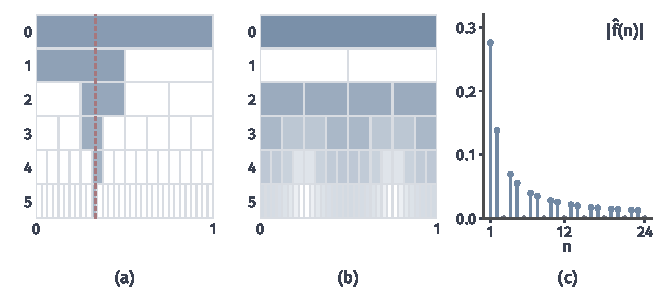
\includegraphics[width=112mm]{figures/04-spaces-measures-and-geometry/03-function-spaces/matplotlib/wavelet-coefficient-tiles/figure.pdf}
  \caption{两种坐标下的系数分布。(a)(b)的每个方格是一个Haar细节系数：纵向为尺度$j$，横向为位置；颜色越深绝对值越大（对数色阶，$10^{-3}$至$1$），白色表示为零。(a)是跳跃函数$\mathbf 1_{[1/3,1)}$，每层只有含跳跃点的一格非零，红色虚线标出$x=1/3$。(b)是$\sin(2\pi x)$，第$1$层全为零，更细的层全部非零。(c)是跳跃函数的Fourier系数绝对值，$n$为$3$的倍数时为零。}
  \label{fig:wavelet-coefficient-tiles}
\end{BookInlineFigure}

\paragraph{平滑振荡}
取$g(x)=\sin(2\pi x)$，$\lVert g\rVert_2^2=1/2$。由$\sin(2\pi x)=(e_1-e_{-1})/(2\mathrm i)$，Fourier系数只有两个非零：
\[
 \hat g(1)=-\frac{\mathrm i}2,\qquad\hat g(-1)=\frac{\mathrm i}2.
\]
两项就精确表示了$g$。

Haar系数则遍布各层。粗项$\int_0^1g=0$。对第$j$层区间$[a,a+h)$，$h=2^{-j}$，记中点$m=a+h/2$，由和差化积，
\begin{equation*}
\begin{aligned}
 \int_a^{m}g-\int_m^{a+h}g
 &=\frac{\cos2\pi a+\cos2\pi(a+h)-2\cos2\pi m}{2\pi}\\
 &=-\frac{2}{\pi}\cos(2\pi m)\sin^2\frac{\pi h}{2}.
\end{aligned}
\end{equation*}
乘以$2^{j/2}$，就得到
\begin{equation}
 d_{j,k}=-\frac{2}{\pi}\,2^{j/2}\cos(2\pi m_{j,k})\sin^2\bigl(\pi2^{-j-1}\bigr).
 \label{eq:wavelet-sine-coefficients}
\end{equation}

逐层读这个公式。$j=0$时$m=1/2$，$d_{0,0}=2/\pi$。$j=1$时两个中点$1/4,3/4$处余弦为零，这一层全为零，因为$g$在每个半周期内关于中点对称。$j\geq2$时中点$(2k+1)2^{-j-1}$都不是$1/4$或$3/4$，这一层的$2^j$个系数全不为零，量级约为$(\pi/2)2^{-3j/2}$，与定理~\ref{thm:wavelet-moment-decay}的Haar估计一致。

\paragraph{局部跳跃}
取$f=\mathbf{1}_{[1/3,1)}$，$\lVert f\rVert_2^2=2/3$。Fourier系数$\hat f(0)=2/3$，$n\neq0$时
\[
 \hat f(n)=\int_{1/3}^1e^{-2\pi\mathrm inx}\,dx=\frac{e^{-2\pi\mathrm in/3}-1}{2\pi\mathrm in}.
\]
取绝对值，得到
\[
 \lvert\hat f(n)\rvert=\frac{\lvert\sin(\pi n/3)\rvert}{\pi\lvert n\rvert}.
\]
$n$是$3$的倍数时为零，其余时为$\sqrt3/(2\pi\lvert n\rvert)$。一处跳跃使无穷多个频率的系数非零，只按$1/\lvert n\rvert$衰减。

Haar系数则高度集中。粗项为$2/3$。若$f$在第$j$层区间上取常值，那里的细节为零，所以每一层只有包含$1/3$的那个区间给出非零系数。沿用第~\ref{sec:wavelet-coefficients-reconstruction}小节的$t_j$：$t_j=1/3$时，$1/3$落在左半，左半减右半的积分是$h/6-h/2=-h/3$；$t_j=2/3$时落在右半，积分是$0-h/3=-h/3$。

于是每层恰有一个非零系数：
\begin{equation}
 d_{j,k}=-2^{j/2}\cdot\frac{h}{3}=-\frac{2^{-j/2}}3.
 \label{eq:wavelet-jump-coefficients}
\end{equation}
能量核对为
\[
 \Bigl(\frac23\Bigr)^2+\sum_{j\geq0}\frac{2^{-j}}9=\frac49+\frac29=\frac23.
\]

\paragraph{有限项的误差}
表~\ref{tab:wavelet-fourier-haar-budget}列出保留部分系数后的平方误差，误差等于被丢弃系数的平方和。Fourier一列保留$\lvert n\rvert\leq N$的项，Haar一列保留粗项与$j<J$的各层，即$P_Jf$。“非零项数”只计实际非零的系数。数值由上面的系数公式求和得到。

\begin{table}[!htb]
\centering
\caption{跳跃函数$f=\mathbf{1}_{[1/3,1)}$与平滑振荡$g=\sin(2\pi x)$在周期区间上的截断平方误差。Fourier保留$\lvert n\rvert\leq N$，Haar保留$V_J$中的全部系数。}
\label{tab:wavelet-fourier-haar-budget}
\begin{tabular}{lccc}
\toprule
表示与截断 & 保留项数 & $f$的非零项数 & $f$的平方误差\\
\midrule
Fourier，$N=4$ & 9 & 7 & 0.0227\\
Fourier，$N=32$ & 65 & 45 & 0.00307\\
Haar，$J=6$ & 64 & 7 & 0.00347\\
\midrule
表示与截断 & 保留项数 & $g$的非零项数 & $g$的平方误差\\
\midrule
Fourier，$N=1$ & 3 & 2 & 0\\
Haar，$J=3$ & 8 & 5 & 0.0252\\
Haar，$J=6$ & 64 & 61 & 0.000401\\
\bottomrule
\end{tabular}
\end{table}

\paragraph{读表}
对跳跃函数，若按固定的项数预算比较，$J=6$的Haar用$64$个位置得到$0.00347$，$N=32$的Fourier用$65$个位置得到$0.00307$，两者相当：线性地截掉高频或细层，误差都大致与项数成反比。

差别出现在“只保留非零系数”时。Haar的$64$个位置中只有$7$个非零，而Fourier要达到同样的误差需要几十个非零项；同样用$7$个非零系数，Haar的误差是$0.00347$，Fourier的误差是$0.0227$。不过，Haar的这一优势要求事先知道跳跃的位置，或者按系数大小自适应地选择保留哪些项。

对平滑振荡，结论反过来：Fourier两项精确表示，Haar在$64$个位置上仍有误差，并且误差每加一层只缩小约四倍，因为Haar只有一个消失矩。换用更光滑、消失矩更多的小波，每层误差下降会更快，但仍不能用有限项精确表示一个正弦。

这说明，正如$\mathbb R^N$中同一个向量在一组基下可能稀疏、在另一组基下可能稠密，函数的稀疏性也不是函数本身的性质，而是函数和基的搭配。哪种表示误差更小，取决于函数（全局振荡还是局部突变）、所用的基以及预算的计法（固定位置还是自适应选取）。这种依赖关系的一般刻画属于第~\ref{chap:function-approximation}章的函数逼近问题。

\section{本章小结}
\label{sec:wavelet-summary}

本章要找一种坐标，让平稳区域的细节接近零，让局部跳变只影响少数系数。小波系数是把函数这条无限维向量换到多尺度标准正交基后读出的坐标，它按尺度$j$和位置$k$排成一张数表。

有限Haar变换给出最简单的回答：对$2^J$个取值反复求平均与半差，得到一个总平均和$2^J-1$个按尺度、位置排列的差值，一处改动在每一层只影响一个系数。把平均与半差乘以$\sqrt2$，变换成为正交矩阵，矩阵的各行就是新的基向量，系数的平方和等于原向量的平方和，逆变换就是转置。

放回区间上，有限变换就是在分段常数函数空间$V_J$中更换标准正交基。到$V_j$的投影是取区间平均；细节空间$W_j=V_{j+1}\cap V_j^{\perp}$由Haar函数张成，记录较粗表示中缺少的左右差异。取值向量要乘以$2^{-J/2}$才是$L^2$坐标，此时保持的是函数的平方积分。

二进阶梯函数在$L^2([0,1])$中稠密，所以粗项加上全部细节构成标准正交基，部分和就是区间平均$P_Jf$，按$L^2$收敛并满足Parseval等式。区间上的粗项不能省略；连续函数的部分和一致收敛，跳跃函数的部分和不一致收敛。

实轴上，正交多分辨率分析把这些结构抽象成嵌套、缩放、平移基、稠密与分离几条要求。尺度函数通过二尺度关系连接相邻层，母小波由二尺度系数写出，证明的关键是把序列按奇偶分成两路，在每个频率上得到$\mathbb C^2$的一组标准正交基。实轴上每层有无限多个位置，粗项在起始层趋于$-\infty$时消失。

消失矩让局部的低次多项式不留痕迹，光滑函数的细节系数因而随层数快速衰减：对$x^2$，Haar的系数是$2^{-3j/2}$的阶，D4的系数精确等于$-(\sqrt3/8)2^{-5j/2}$。小波的光滑性则决定有限项重构是否光滑。

有限区间要处理跨越端点的基函数。周期化给出周期函数空间的标准正交基，零阶矩保留而高阶矩在跨接缝处失效。周期延拓是$L^2$等距同构，却可能在接缝处产生跳跃或折角；反射延拓能消除取值跳跃而不保证导数连续；边界小波在区间内重新构造端点附近的基函数，需要重新核对正交、完备与消失矩。

与Fourier系数比较，全局振荡适合频率坐标，局部跳跃适合尺度位置坐标，哪种误差更小取决于函数、基和预算的计法。截断误差的定量刻画在第~\ref{chap:function-approximation}章研究；第~\ref{chap:besov-spaces}章在本章的周期边界设定下，用小波系数在各层上的大小定义和刻画函数的正则性。


\chapter{线性泛函}
\label{chap:linear-functionals}
\label{chap:linear-functionals-operators}

研究一个函数时，我们常常只读出一个数：它在某段区间上的平均，它的某个Fourier系数，它在某一点的取值。这样的读数把整个函数变成一个标量。不同读数的可靠程度不同：函数稍有扰动，平均值只变一点，而一个点上的值可能被一个窄尖峰完全改变。哪些读数能由函数的范数稳定地控制，这些读数长什么样，能否从局部扩展到整个空间，是本章的第一组问题。

本章先把函数空间到标量的映射称为泛函，用积分、系数和点值比较线性与非线性读数，再用一个常数界刻画线性泛函的连续性，定义泛函范数。全部连续线性泛函组成对偶空间；在Hilbert空间中它们都是内积，在$L^p$空间中它们都是加权积分。对一般的赋范空间写不出这样的表示，Hahn--Banach定理转而保证子空间上的读数能保持范数地延拓到全空间，由此连续线性读数足以区分不同的向量并读出范数。完备性还给出另一种统一控制：逐个向量有界的泛函族在范数上一致有界。

第二组问题从范数误差转向读数。若一列向量在每个连续线性读数下都收敛，称为弱收敛；在对偶空间中只用原空间的向量去读，称为弱星收敛。我们说明它们与范数收敛的区别、它们仍然控制的范数界，以及在什么条件下有界序列一定有这样收敛的子列。无限维空间中闭球在范数下不紧，第~\ref{chap:functions-as-vectors}章已经看到这一困难；弱星与弱拓扑下的紧性，是绕开它的标准办法。

本章只讨论输出为标量的线性映射。输出为向量的有界线性算子、算子范数、伴随与一般的算子定理在第~\ref{chap:linear-operators}章建立；以泛函为目标的变分与优化由卷五承担。全章的拓扑与度量语言来自第~\ref{chap:topological-spaces}章至第~\ref{chap:metric-space-maps}章，具体空间来自第~\ref{chap:normed-spaces}章和第~\ref{chap:inner-product-spaces}章。

\section{泛函的定义}
\label{sec:lfunc-definition}

函数空间中的元素是整个函数，我们对它所做的许多操作最后只得到一个数。把这类操作统一起来，就得到泛函的概念。本节先看几个常见的例子，逐一核对它们是否线性、在哪个空间上有定义；再研究线性泛函什么时候连续，并用一个数度量它把输入误差放大多少。全章记标量域为$\mathbb F$，它是$\mathbb R$或$\mathbb C$。

\begin{definition}[泛函]
\label{def:lfunc-functional}
设$X$是$\mathbb F$上的线性空间。映射$\ell:X\to\mathbb F$称为$X$上的\term{泛函}（functional）。若对一切$x,y\in X$和$\alpha,\beta\in\mathbb F$都有$\ell(\alpha x+\beta y)=\alpha\ell(x)+\beta\ell(y)$，称$\ell$为\term{线性泛函}（linear functional）。
\end{definition}

有限维空间上的线性泛函由它在一组基上的取值决定，可以写成坐标的线性组合，这在\BookChapterRef{chap:linear-representation}{卷二第2章“线性空间、映射与坐标”}中已经讨论过。函数空间是无限维的，新问题在于：线性泛函未必连续，读数是否稳定要看空间所配的范数。

\subsection{常见泛函}
\label{sec:lfunc-examples}

下面四个例子分别代表加权平均、坐标读取、点上取值和能量。每个例子都要先说清它作用在哪个空间上，因为同一条规则在一个空间上有意义，在另一个空间上可能根本没有定义。

\paragraph{加权积分}
设$(\Omega,\mathcal F,\mu)$是测度空间，$1\leq p\leq\infty$，$q$是\term{共轭指数}（conjugate exponent），即$1/p+1/q=1$，约定$p=1$时$q=\infty$、$p=\infty$时$q=1$。对固定的$g\in L^q(\mu)$，令
\begin{equation}
L_g(f)=\int_\Omega fg\,d\mu\qquad(f\in L^p(\mu)).
\label{eq:lfunc-weighted-integral}
\end{equation}
由第~\ref{chap:normed-spaces}章的Hölder不等式，$\int\lvert fg\rvert\,d\mu\leq\lVert f\rVert_p\lVert g\rVert_q<\infty$，积分有定义。线性来自积分的线性：$L_g(\alpha f_1+\beta f_2)=\alpha L_g(f_1)+\beta L_g(f_2)$。

$L^p$的元素是几乎处处相等的函数组成的等价类，所以还要检查读数不依赖代表的选取。若$f=\tilde f$几乎处处成立，则$fg=\tilde fg$几乎处处成立，两者的积分相同。积分对零测集不敏感，这正是加权积分能在等价类上使用的原因。

\paragraph{正交系数}
设$H$是Hilbert空间，$\{e_k\}$是标准正交系。第$k$个系数$f\mapsto\langle e_k,f\rangle$是$H$上的泛函；按第~\ref{chap:inner-product-spaces}章的约定，内积对第二个变量线性，所以它是线性泛函。在$L^2(0,1)$中，它就是以$\overline{e_k}$为权重的加权积分。

\paragraph{点评估}
设$K$是紧度量空间，$C(K)$是$K$上的连续函数空间。固定$x_0\in K$，令$\delta_{x_0}(f)=f(x_0)$，称为$x_0$处的\term{点评估泛函}（point evaluation functional）。它显然是线性的。

点评估要求逐点取值，只在由真正的函数组成的空间上有定义。在Lebesgue测度下的$L^p(0,1)$中，单点$\{x_0\}$的测度为零，$f$与$f+\mathbf{1}_{\{x_0\}}$属于同一个等价类，在$x_0$处的值却不同。所以“读出$x_0$处的值”不是$L^p$上的映射，谈不上线性或连续。积分与点评估的区别就在这里：前者对零测集不敏感，后者恰恰只看一个零测集。

\paragraph{平方范数}
在赋范空间上，$f\mapsto\lVert f\rVert^2$也把函数变成一个数，例如$L^2$中的能量$\int\lvert f\rvert^2$。它不是线性的：$\lVert2f\rVert^2=4\lVert f\rVert^2\neq2\lVert f\rVert^2$（$f\neq0$时）。非线性泛函在优化中很常见，如以函数为未知量的能量与损失；它们的变分和极小化可参考\BookChapterRef{chap:functional-optimization-variation}{卷五第11章“泛函优化与变分”}。本章只研究线性泛函。

\subsection{泛函范数}
\label{sec:lfunc-norm}

读数是否稳定，就是输入的小误差是否只引起读数的小误差。对线性泛函，这个要求有简单的等价形式。设$X$是赋范空间。由第~\ref{chap:metric-space-maps}章的距离判据，$\ell$在$x_0$处连续，意思是对每个$\varepsilon>0$存在$\delta>0$，使$\lVert x-x_0\rVert<\delta$时$\lvert\ell(x)-\ell(x_0)\rvert<\varepsilon$。

\begin{theorem}[线性泛函的连续性]
\label{thm:lfunc-continuity-bounded}
设$X$是赋范空间，$\ell$是$X$上的线性泛函。以下三条等价：
\begin{enumerate}
\item $\ell$在$0$处连续；
\item $\ell$在$X$上处处连续；
\item 存在常数$C\geq0$，使$\lvert\ell(x)\rvert\leq C\lVert x\rVert$对一切$x\in X$成立。
\end{enumerate}
\end{theorem}

\begin{proof}
由3推2：$\lvert\ell(x)-\ell(x_0)\rvert=\lvert\ell(x-x_0)\rvert\leq C\lVert x-x_0\rVert$，取$\delta=\varepsilon/(C+1)$即可。由2推1是显然的。

由1推3：取$\varepsilon=1$，由$\ell(0)=0$，存在$\delta>0$使$\lVert z\rVert<\delta$时$\lvert\ell(z)\rvert<1$。对$x\neq0$，令$z=\frac{\delta}{2\lVert x\rVert}x$，则$\lVert z\rVert=\delta/2<\delta$，于是由线性
\[
\lvert\ell(x)\rvert=\frac{2\lVert x\rVert}{\delta}\lvert\ell(z)\rvert<\frac{2}{\delta}\lVert x\rVert .
\]
$x=0$时不等式两边都是零。取$C=2/\delta$。
\end{proof}

线性在证明中起了两次作用：把任意点处的误差平移成原点附近的误差，把原点附近的控制按比例放大到所有向量。满足第3条的线性泛函称为\term{有界线性泛函}（bounded linear functional）；由定理~\ref{thm:lfunc-continuity-bounded}，对线性泛函而言“有界”与“连续”是同一回事。这里的有界指在单位球上有界，而不是在整个空间上有界，后者只有零泛函才满足。

\begin{definition}[泛函范数]
\label{def:lfunc-functional-norm}
设$\ell$是赋范空间$X$上的有界线性泛函，令
\[
\lVert\ell\rVert=\sup_{\lVert x\rVert\leq1}\lvert\ell(x)\rvert,
\]
称为$\ell$的\term{泛函范数}（norm of a functional）。
\end{definition}

由线性，$\lvert\ell(x)\rvert\leq\lVert\ell\rVert\lVert x\rVert$对一切$x$成立，并且$\lVert\ell\rVert$是使这一不等式成立的最小常数$C$。它衡量的是读数对输入误差的最大放大倍数。

\paragraph{点评估的范数依赖空间}
在$C([0,1])$上配一致范数$\lVert f\rVert_\infty=\max\lvert f\rvert$，由$\lvert f(0)\rvert\leq\lVert f\rVert_\infty$得$\lVert\delta_0\rVert\leq1$，取$f\equiv1$得$\lVert\delta_0\rVert=1$。点评估在一致范数下是稳定的读数。

同一个集合$C([0,1])$改配积分范数，结论完全不同。取贴着左端点的尖峰
\[
\tau_n(t)=\max(1-nt,0)\qquad(t\in[0,1]),
\]
它连续，$\tau_n(0)=1$，而直接积分得
\[
\lVert\tau_n\rVert_1=\int_0^{1/n}(1-nt)\,dt=\frac{1}{2n},\qquad
\lVert\tau_n\rVert_2^2=\int_0^{1/n}(1-nt)^2\,dt=\frac{1}{3n}.
\]
两种积分范数都趋于零，读数却始终是$1$，所以不存在常数$C$使$\lvert f(0)\rvert\leq C\lVert f\rVert_2$对一切连续$f$成立。在$(C([0,1]),\lVert\cdot\rVert_2)$上，$\delta_0$是线性的、处处有定义，却不连续。

\paragraph{加权积分的范数也依赖空间}
在$L^2(0,1)$上取$g=\mathbf{1}_{[0,1/2]}$，$L_g(f)=\int_0^{1/2}f$。Hölder不等式给出$\lVert L_g\rVert\leq\lVert g\rVert_2=1/\sqrt2$；取$f=g$，$L_g(g)=1/2$而$\lVert g\rVert_2=1/\sqrt2$，比值为$1/\sqrt2$，所以$\lVert L_g\rVert=1/\sqrt2$。同一规则在$C([0,1])$的一致范数下，由$\lvert\int_0^{1/2}f\rvert\leq\lVert f\rVert_\infty/2$及$f\equiv1$得范数为$1/2$。读数规则相同，范数不同，因为衡量输入误差的方式不同。是否稳定、放大多少，都依赖所选的空间与范数。

\section{泛函的表示}
\label{sec:lfunc-representation}

上一节逐个研究读数规则。现在把同一空间上全部连续线性读数收集起来，看它们组成怎样的空间，以及在具体空间中它们能否写成熟悉的形式。先建立对偶空间及其范数，并证明它总是完备的；再分别在Hilbert空间和$L^p$空间中证明，每个连续线性泛函都是内积或加权积分，表示唯一，并且泛函范数等于表示对象的范数。

\subsection{对偶空间}
\label{sec:lfunc-dual-space}

两个有界线性泛函之和、数乘仍是有界线性泛函，所以它们组成一个线性空间，泛函范数是这个空间上的范数：三角不等式来自$\lvert(\ell_1+\ell_2)(x)\rvert\leq\lvert\ell_1(x)\rvert+\lvert\ell_2(x)\rvert$再对单位球取上确界。

\begin{definition}[对偶空间与二次对偶空间]
\label{def:lfunc-dual-space}
赋范空间$X$上全部有界线性泛函组成的空间记为$X^*$，配以泛函范数，称为$X$的\term{对偶空间}（dual space）。$X^*$本身是赋范空间，它的对偶空间$X^{**}=(X^*)^*$称为$X$的\term{二次对偶空间}（bidual space）。
\end{definition}

对偶空间的元素是读数规则，二次对偶空间的元素是“读数规则的读数规则”：给它一个$X$上的泛函，它返回一个数。第~\ref{sec:lfunc-reflexivity}小节会看到，每个$x\in X$都以$\ell\mapsto\ell(x)$的方式自然地成为$X^{**}$的元素；比较这些元素与$X^{**}$的全部元素，是后面讨论弱拓扑与紧性的基础。

\paragraph{对偶范数可以不同于原范数}
即使在有限维中，对偶空间的范数也可以与原空间的范数形式不同。在$\mathbb R^2$上配$\lVert\bm x\rVert_1=\lvert x_1\rvert+\lvert x_2\rvert$。每个线性泛函都写成$\ell(\bm x)=a_1x_1+a_2x_2$，由
\[
\lvert\ell(\bm x)\rvert\leq\max(\lvert a_1\rvert,\lvert a_2\rvert)\bigl(\lvert x_1\rvert+\lvert x_2\rvert\bigr)
\]
且在$\bm x=\bm e_1$或$\bm e_2$处取到等号，得$\lVert\ell\rVert=\max(\lvert a_1\rvert,\lvert a_2\rvert)$。系数向量$\bm a$作为读数的长度要用最大值范数计算，这是\term{对偶范数}（dual norm）的一个例子。所以不能把读数规则与表示它的系数向量随意等同，除非已经核对了范数。

\paragraph{对偶空间总是完备的}
对偶空间有一个原空间未必具有的性质：无论$X$本身是否完备，$X^*$都完备。原因是读数取值在完备的$\mathbb F$中。

\begin{theorem}[对偶空间的完备性]
\label{thm:lfunc-dual-complete}
对任意赋范空间$X$，$X^*$是Banach空间。
\end{theorem}

\begin{proof}
设$(\ell_n)$是$X^*$中的Cauchy列。对每个$x$，$\lvert\ell_n(x)-\ell_m(x)\rvert\leq\lVert\ell_n-\ell_m\rVert\lVert x\rVert$，所以$(\ell_n(x))$是$\mathbb F$中的Cauchy列，有极限，记为$\ell(x)$。极限保持线性，$\ell$是线性泛函。

给定$\varepsilon>0$，取$N$使$n,m\geq N$时$\lVert\ell_n-\ell_m\rVert<\varepsilon$。对$\lVert x\rVert\leq1$，$\lvert\ell_n(x)-\ell_m(x)\rvert<\varepsilon$；令$m\to\infty$得$\lvert\ell_n(x)-\ell(x)\rvert\leq\varepsilon$。所以$\lvert\ell(x)\rvert\leq\lVert\ell_N\rVert+\varepsilon$在单位球上成立，$\ell$有界，属于$X^*$；并且$n\geq N$时$\lVert\ell_n-\ell\rVert\leq\varepsilon$，即$\ell_n\to\ell$。
\end{proof}

例如由多项式组成的不完备空间配上一致范数，它的对偶空间仍是Banach空间。这一性质在第~\ref{sec:lfunc-uniform-boundedness}节和第~\ref{sec:lfunc-weak-norm-control}小节中起关键作用：需要完备性的论证，可以在$X^*$上进行而不必要求$X$完备。

\subsection{Hilbert空间的泛函表示}
\label{sec:lfunc-riesz}

在Hilbert空间$H$中，每个向量都给出一个读数。按第~\ref{chap:inner-product-spaces}章的约定，复内积对第一个变量共轭线性、对第二个变量线性。对$h\in H$令$\ell_h(f)=\langle h,f\rangle$，它对$f$线性；由Cauchy--Schwarz不等式，$\lvert\ell_h(f)\rvert\leq\lVert h\rVert\lVert f\rVert$，所以$\lVert\ell_h\rVert\leq\lVert h\rVert$。$h\neq0$时取$f=h/\lVert h\rVert$，读数为$\lVert h\rVert$，于是$\lVert\ell_h\rVert=\lVert h\rVert$。

反过来的问题更有用：给定连续线性泛函$\ell$，是否一定有向量$h$使$\ell=\ell_h$？若是，读数就可以用空间中的几何来研究，读数的范数就是一个向量的长度。

\paragraph{零空间与正交方向}
零泛函由零向量表示。设$\ell\neq0$，考察它的零空间$N=\{f:\ell(f)=0\}$。它是线性子空间；又由连续性，若$f_n\in N$且$f_n\to f$，则$\ell(f)=\lim\ell(f_n)=0$，所以$N$是闭子空间，且$N\neq H$。若能找到与$N$正交的非零向量$w$，读数就只取决于$f$沿$w$方向的分量，表示向量应当是$w$的某个倍数。由此得到的结论称为\term{Riesz表示定理}（Riesz representation theorem）。

\begin{theorem}[Riesz表示定理]
\label{thm:lfunc-riesz}
设$H$是Hilbert空间，$\ell\in H^*$。则存在唯一的$h_\ell\in H$，使
\begin{equation}
\ell(f)=\langle h_\ell,f\rangle\qquad(f\in H),
\label{eq:lfunc-riesz}
\end{equation}
并且$\lVert\ell\rVert=\lVert h_\ell\rVert$。
\end{theorem}

\begin{proof}
$\ell=0$时取$h_\ell=0$。下设$\ell\neq0$，$N$如上。

\emph{找与零空间正交的方向。}取$v$使$\ell(v)\neq0$。由第~\ref{chap:inner-product-spaces}章的正交投影定理，$v=Pv+w$，其中$Pv\in N$，$w\perp N$。由$\ell(w)=\ell(v)-\ell(Pv)=\ell(v)\neq0$知$w\neq0$。

\emph{写出表示。}对任意$f\in H$，向量$f-\frac{\ell(f)}{\ell(w)}w$在$\ell$下的值为零，属于$N$，因而与$w$正交：
\[
0=\Bigl\langle w,f-\frac{\ell(f)}{\ell(w)}w\Bigr\rangle=\langle w,f\rangle-\frac{\ell(f)}{\ell(w)}\lVert w\rVert^2 .
\]
这里用到内积对第二个变量线性。解出$\ell(f)=\frac{\ell(w)}{\lVert w\rVert^2}\langle w,f\rangle$。令$h_\ell=\frac{\overline{\ell(w)}}{\lVert w\rVert^2}w$，由内积对第一个变量共轭线性，$\langle h_\ell,f\rangle=\frac{\ell(w)}{\lVert w\rVert^2}\langle w,f\rangle=\ell(f)$。

\emph{唯一性与范数。}若$h,h'$都满足式~\eqref{eq:lfunc-riesz}，则$\langle h-h',f\rangle=0$对一切$f$成立，取$f=h-h'$得$h=h'$。范数等式是本小节开头对$\ell_h$的计算。
\end{proof}

证明只用了正交投影定理，而正交投影定理对任意Hilbert空间中的闭子空间成立，所以Riesz表示定理不要求$H$可分，也不需要事先选取正交基。表示向量公式中的共轭使对应$\ell\mapsto h_\ell$在复空间中是共轭线性的：$h_{\alpha\ell}=\bar\alpha h_\ell$。实空间中这个共轭消失，$H^*$与$H$通过保范数的线性双射等同。

\paragraph{\texorpdfstring{$L^2$}{L2}中的读数与方向}
在$L^2(0,1)$中，几个读数的表示向量可以直接写出。整体平均$\ell(f)=\int_0^1f$对应$h_\ell=1$，范数为$1$。加权读数$\ell(f)=\int_0^1tf(t)\,dt$对应$h_\ell(t)=t$，范数为$(\int_0^1t^2\,dt)^{1/2}=1/\sqrt3$。第$k$个正交系数$f\mapsto\langle e_k,f\rangle$对应$h_\ell=e_k$。

\paragraph{表示以连续性为前提}
定理不能替一条读数规则证明连续性。点评估在$L^2(0,1)$上根本没有定义；在$(C([0,1]),\lVert\cdot\rVert_2)$上它有定义但不连续，也确实没有表示向量：若有$h$使$f(0)=\langle h,f\rangle$对一切连续$f$成立，代入尖峰$\tau_n$，左端恒为$1$，右端不超过$\lVert h\rVert_2\lVert\tau_n\rVert_2\to0$，矛盾。完备性也不能省：$(C([0,1]),\lVert\cdot\rVert_2)$上的有界读数$\int_0^{1/2}f$在完备化$L^2(0,1)$中的表示向量是$\mathbf{1}_{[0,1/2]}$，它没有连续代表，所以在不完备的空间中找不到表示向量。

若某个函数空间配上内积后完备，并且点评估在其中连续，Riesz表示定理就把点评估写成与某个固定函数的内积。第~\ref{chap:rkhs}章研究的再生核Hilbert空间正是这样的空间。

\subsection{\texorpdfstring{$L^p$}{Lp}空间的泛函表示}
\label{sec:lfunc-lp-dual}

在$L^p$中没有内积可用，自然的候选是加权积分~\eqref{eq:lfunc-weighted-integral}。第~\ref{sec:lfunc-examples}小节已说明每个$g\in L^q$给出有界读数$L_g$，且$\lVert L_g\rVert\leq\lVert g\rVert_q$。本小节回答反方向的问题。为了不处理共轭记号，下面在实值函数上证明；复值情形对实部与虚部分别处理，结论相同，只是$p=2$时$L_g$的表示向量在内积记号下是$\bar g$。

\begin{theorem}[$L^p$的对偶表示]
\label{thm:lfunc-lp-dual}
设$(\Omega,\mathcal F,\mu)$是$\sigma$有限测度空间，$1\leq p<\infty$，$q$为共轭指数。则每个$\ell\in(L^p(\mu))^*$都存在$g\in L^q(\mu)$使$\ell=L_g$；$g$在几乎处处相等的意义下唯一，并且$\lVert\ell\rVert=\lVert g\rVert_q$。
\end{theorem}

证明分三步：先说明$\lVert L_g\rVert$恰好等于$\lVert g\rVert_q$，从而表示唯一；再在有限测度下由读数构造测度并用Radon--Nikodym定理得到$g$；最后推广到$\sigma$有限测度。

\paragraph{范数等式与唯一性}
设$1<p<\infty$，$g\neq0$。令$f=\lvert g\rvert^{q-1}\operatorname{sgn}g$，则$fg=\lvert g\rvert^q$，又因$(q-1)p=q$，$\lvert f\rvert^p=\lvert g\rvert^q$。于是$L_g(f)=\lVert g\rVert_q^q$，$\lVert f\rVert_p=\lVert g\rVert_q^{q/p}$，比值为$\lVert g\rVert_q^{q-q/p}=\lVert g\rVert_q$。$p=1$、$q=\infty$时等号未必取到，改用逼近：对$0<\varepsilon<\lVert g\rVert_\infty$，集合$E=\{\lvert g\rvert>\lVert g\rVert_\infty-\varepsilon\}$测度为正；由$\sigma$有限，可取$E$中测度有限且为正的部分$E'$，令$f=\operatorname{sgn}(g)\mathbf{1}_{E'}/\mu(E')$，则$\lVert f\rVert_1=1$而$L_g(f)\geq\lVert g\rVert_\infty-\varepsilon$。两种情形都得到$\lVert L_g\rVert=\lVert g\rVert_q$。

由此表示是唯一的：若$L_g=L_{g'}$，则$L_{g-g'}=0$，其范数$\lVert g-g'\rVert_q=0$，即$g=g'$几乎处处成立。表示函数只确定到几乎处处相等，这与$L^q$的元素本来就是等价类一致。

\paragraph{有限测度下构造表示函数}
先设$\mu(\Omega)<\infty$。给定$\ell\in(L^p)^*$，对可测集$E$令$\nu(E)=\ell(\mathbf{1}_E)$。有限可加性来自线性。可数可加性来自连续性，这里用到$p<\infty$：若$E=\bigcup_kE_k$为不交并，则
\[
\Bigl\lVert\mathbf{1}_E-\sum_{k\leq n}\mathbf{1}_{E_k}\Bigr\rVert_p=\mu\Bigl(\bigcup_{k>n}E_k\Bigr)^{1/p}\to0,
\]
所以$\sum_{k\leq n}\nu(E_k)\to\nu(E)$。又$\lvert\nu(E)\rvert\leq\lVert\ell\rVert\mu(E)^{1/p}$，$\nu$是有限的有符号测度，并且$\mu(E)=0$时$\nu(E)=0$，即$\nu$对$\mu$绝对连续。

由第~\ref{chap:measure}章，有限的有符号测度可分解为两个有限测度之差，它们都对$\mu$绝对连续；分别应用第~\ref{chap:measure-densities}章的Radon--Nikodym定理，得到$g\in L^1(\mu)$使$\ell(\mathbf{1}_E)=\int_Eg\,d\mu$对一切可测集$E$成立。由线性，$\ell(f)=\int fg\,d\mu$对一切简单函数$f$成立。

\paragraph{表示函数属于\texorpdfstring{$L^q$}{Lq}}
设$1<p<\infty$。令$E_n=\{\lvert g\rvert\leq n\}$，$f_n=\lvert g\rvert^{q-1}\operatorname{sgn}(g)\mathbf{1}_{E_n}$。$f_n$是有界可测函数，可以被简单函数一致逼近；在有限测度下一致收敛推出$L^p$收敛，而$\ell$连续、$g$可积，所以等式$\ell(f_n)=\int f_ng\,d\mu$也成立。于是
\[
\int_{E_n}\lvert g\rvert^q\,d\mu=\ell(f_n)\leq\lVert\ell\rVert\lVert f_n\rVert_p=\lVert\ell\rVert\Bigl(\int_{E_n}\lvert g\rvert^q\,d\mu\Bigr)^{1/p},
\]
整理得$(\int_{E_n}\lvert g\rvert^q)^{1/q}\leq\lVert\ell\rVert$，由单调收敛定理令$n\to\infty$得$\lVert g\rVert_q\leq\lVert\ell\rVert$。

设$p=1$。若$F=\{g>\lVert\ell\rVert\}$测度为正，取$f=\mathbf{1}_F/\mu(F)$，则$\lVert f\rVert_1=1$，而$\ell(f)=\frac{1}{\mu(F)}\int_Fg\,d\mu>\lVert\ell\rVert$，矛盾；对$\{g<-\lVert\ell\rVert\}$同理。所以$\lVert g\rVert_\infty\leq\lVert\ell\rVert$。

两种情形下$g\in L^q$，$\ell$与$L_g$都是$L^p$上的连续线性泛函，在简单函数上相等。由第~\ref{chap:normed-spaces}章，简单函数在$L^p$（$p<\infty$）中稠密，两个连续函数在稠密集上相等则处处相等，所以$\ell=L_g$。

\paragraph{推广到\texorpdfstring{$\sigma$}{sigma}有限测度}
设$\Omega=\bigcup_k\Omega_k$，$\Omega_k$两两不交且测度有限。把$\ell$限制到在$\Omega_k$外为零的函数上，由有限测度情形得到$\Omega_k$上的$g_k$，令$g=\sum_kg_k\mathbf{1}_{\Omega_k}$。对$A_n=\Omega_1\cup\cdots\cup\Omega_n$，同样的论证给出$\lVert g\mathbf{1}_{A_n}\rVert_q\leq\lVert\ell\rVert$，由单调收敛得$\lVert g\rVert_q\leq\lVert\ell\rVert$。于是$\ell$与$L_g$在支撑于某个$A_n$内的简单函数上相等，这些函数在$L^p$中仍稠密，所以$\ell=L_g$。$p=1$时$\sigma$有限的假设不能去掉；$1<p<\infty$时可以用更细的论证去掉，这里不展开。

\begin{example}[一个可复算的对偶范数]
\label{ex:lfunc-l3-norm}
在$L^3(0,1)$上取$\ell(f)=\int_0^1tf(t)\,dt$。共轭指数$q=3/2$，由定理~\ref{thm:lfunc-lp-dual}，
\[
\lVert\ell\rVert=\Bigl(\int_0^1t^{3/2}\,dt\Bigr)^{2/3}=\Bigl(\frac25\Bigr)^{2/3}\approx0.543,
\]
取到范数的输入是$f(t)=t^{q-1}=t^{1/2}$：$\ell(t^{1/2})=\int_0^1t^{3/2}=2/5$，$\lVert t^{1/2}\rVert_3=(\int_0^1t^{3/2})^{1/3}=(2/5)^{1/3}$，比值为$(2/5)^{2/3}$。同一个权重在$L^2$中的读数范数是$\lVert t\rVert_2=1/\sqrt3\approx0.577$，在$L^1$中是$\lVert t\rVert_\infty=1$。
\end{example}

\paragraph{端点\texorpdfstring{$p=\infty$}{p=infinity}}
定理排除了$p=\infty$，这不是技术上的疏忽。每个$g\in L^1$仍给出$L^\infty$上的有界读数$L_g$，但$L^\infty$上的连续线性泛函一般不能全部写成这种形式。第~\ref{sec:lfunc-hahn-banach}小节将用延拓定理在$\ell^\infty$上构造一个不来自任何$\ell^1$序列的连续线性泛函。所以有限维和$L^2$中“对偶就是自身”的直觉，以及$1\leq p<\infty$时“对偶就是$L^q$”的结论，都不能直接用到$L^\infty$上。

\section{泛函的延拓}
\label{sec:lfunc-extension}

一般的赋范空间没有内积，也不是积分空间，上一节的表示定理都用不上，我们甚至不知道$X^*$中是否有足够多的元素。在Hilbert空间中，任何非零向量$x$都被读数$\langle x,\cdot\rangle$识别出来，因为它在$x$处的值是$\lVert x\rVert^2\neq0$。一般空间中写不出这样的读数，但可以先在一个小子空间上定义它，再设法扩展到整个空间，并且不增大它的范数。本节先建立这种延拓，再用它证明连续线性读数能读出范数、区分向量。

\subsection{Hahn--Banach延拓}
\label{sec:lfunc-hahn-banach}

设$M$是$X$的线性子空间，$\ell$是$M$上的有界线性泛函，即$\lvert\ell(m)\rvert\leq\lVert\ell\rVert\lVert m\rVert$对$m\in M$成立。我们要找$L\in X^*$，使$L$在$M$上与$\ell$一致，并且$\lVert L\rVert=\lVert\ell\rVert$。延拓总能保持在$M$上的取值，难点在于不增大范数：$L$在$M$外的取值要受$\lvert L(x)\rvert\leq\lVert\ell\rVert\lVert x\rVert$的约束。

\begin{theorem}[Hahn--Banach定理]
\label{thm:lfunc-hahn-banach}
设$X$是赋范空间，$M\subset X$是线性子空间，$\ell:M\to\mathbb F$是有界线性泛函。则存在$L\in X^*$，使$L|_M=\ell$且$\lVert L\rVert=\lVert\ell\rVert$。
\end{theorem}

这一结论称为\term{Hahn--Banach定理}（Hahn--Banach theorem）。下面先完整证明延拓一维的核心步骤，再说明怎样推广到整个空间。

\paragraph{延拓一维}
设$\mathbb F=\mathbb R$，不妨设$\lVert\ell\rVert=1$（$\ell=0$时取$L=0$，否则除以$\lVert\ell\rVert$）。任取$z\notin M$，要把$\ell$延拓到$M\oplus\operatorname{span}\{z\}$上。线性延拓完全由一个数$t=L(z)$决定：$L(m+sz)=\ell(m)+st$。要求$\lVert L\rVert\leq1$，即
\[
\lvert\ell(m)+st\rvert\leq\lVert m+sz\rVert\qquad(m\in M,\ s\in\mathbb R).
\]
$s=0$时这就是$\lVert\ell\rVert\leq1$。$s\neq0$时两边除以$\lvert s\rvert$，并把$m/s$重新记为$m$，条件化为
\[
-\lVert m+z\rVert-\ell(m)\leq t\leq\lVert m+z\rVert-\ell(m)\qquad(m\in M).
\]

这样的$t$存在，当且仅当左端对$m$的上确界不超过右端对$m'$的下确界，即对一切$m,m'\in M$，
\[
-\lVert m+z\rVert-\ell(m)\leq\lVert m'+z\rVert-\ell(m').
\]
这确实成立：$\ell(m')-\ell(m)=\ell(m'-m)\leq\lVert m'-m\rVert\leq\lVert m'+z\rVert+\lVert m+z\rVert$，移项即得。所以可选的$t$组成一个非空闭区间，任取其中一个，就把$\ell$保范数地延拓了一维。

\paragraph{从一维到全空间}
若$X$可分，取可数稠密集$\{z_1,z_2,\ldots\}$，逐个把$z_k$添入定义域并重复上一步，得到$\operatorname{span}(M\cup\{z_k\}_k)$上范数仍为$\lVert\ell\rVert$的延拓。这个子空间稠密，而有界线性泛函一致连续，可以唯一地连续延拓到闭包即整个$X$上，范数不变：若$x_n\to x$，则$(L(x_n))$是Cauchy列，极限与所选序列无关，且$\lvert L(x)\rvert=\lim\lvert L(x_n)\rvert\leq\lVert\ell\rVert\lVert x\rVert$。不可分时，“逐个添加”要换成对所有保范数延拓按包含关系排序后使用Zorn引理，思路相同，这里不给出这一部分的证明。

\paragraph{复空间}
设$\mathbb F=\mathbb C$。复线性泛函由实部决定：记$u=\operatorname{Re}\ell$，则$\ell(m)=u(m)-\mathrm iu(\mathrm im)$，因为$\operatorname{Im}\ell(m)=-\operatorname{Re}(\mathrm i\ell(m))=-u(\mathrm im)$。把$X$看成实赋范空间，$u$是$M$上的实线性泛函，$\lvert u(m)\rvert\leq\lvert\ell(m)\rvert$，按实情形把$u$延拓为$U$且$\lVert U\rVert\leq\lVert\ell\rVert$，再令$L(x)=U(x)-\mathrm iU(\mathrm ix)$。直接验证$L$复线性且在$M$上等于$\ell$。对每个$x$取$\theta$使$e^{-\mathrm i\theta}L(x)=\lvert L(x)\rvert$，则$\lvert L(x)\rvert=L(e^{-\mathrm i\theta}x)$是实数，等于其实部$U(e^{-\mathrm i\theta}x)\leq\lVert\ell\rVert\lVert x\rVert$。所以$\lVert L\rVert\leq\lVert\ell\rVert$，反向不等式是显然的。

\paragraph{延拓可以不唯一}
一维延拓中的“非空区间”一般不止一点。在$(\mathbb R^2,\lVert\cdot\rVert_1)$中取$M$为横轴，$\ell(s,0)=s$，$\lVert\ell\rVert=1$。延拓写成$L_t(\bm x)=x_1+tx_2$，由第~\ref{sec:lfunc-dual-space}小节的对偶范数计算，$\lVert L_t\rVert=\max(1,\lvert t\rvert)$，所以每个$\lvert t\rvert\leq1$都给出保范数延拓。几何上，直线$x_1+tx_2=1$都经过$(1,0)$并支撑菱形单位球，菱形在这个顶点处有许多支撑线。换成欧氏范数，单位圆在$(1,0)$只有一条切线$x_1=1$，延拓唯一。定理保证的是存在，并且保持的只有两条约束：在$M$上的取值和范数上界，$M$外的取值一般不由它们确定。

\paragraph{区分向量与子空间}
延拓的一个直接用途，是用一个连续线性读数把一个向量与一个闭子空间分开。

\begin{theorem}[距离泛函]
\label{thm:lfunc-distance-functional}
设$M$是赋范空间$X$的闭子空间，$x_0\notin M$，$d=\inf_{m\in M}\lVert x_0-m\rVert$。则$d>0$，并且存在$L\in X^*$，使$\lVert L\rVert=1$，$L$在$M$上为零，$L(x_0)=d$。
\end{theorem}

\begin{proof}
$M$闭而$x_0\notin M$，所以$x_0$有一个邻域与$M$不交，$d>0$。在$M\oplus\operatorname{span}\{x_0\}$上令$\ell(m+sx_0)=sd$。$s\neq0$时$\lVert m+sx_0\rVert=\lvert s\rvert\lVert x_0+m/s\rVert\geq\lvert s\rvert d$，所以$\lvert\ell(m+sx_0)\rvert\leq\lVert m+sx_0\rVert$，$\lVert\ell\rVert\leq1$。取$m_n\in M$使$\lVert x_0-m_n\rVert\to d$，则$\ell(x_0-m_n)=d$，比值趋于$1$，故$\lVert\ell\rVert=1$。由定理~\ref{thm:lfunc-hahn-banach}延拓即得。
\end{proof}

\paragraph{\texorpdfstring{$\ell^\infty$}{l-infinity}上不来自\texorpdfstring{$\ell^1$}{l1}的泛函}
现在可以完成第~\ref{sec:lfunc-lp-dual}小节末尾的说明。记$c$为$\ell^\infty$中收敛数列组成的子空间，在其上令$\lambda(x)=\lim_nx_n$。由$\lvert\lim x_n\rvert\leq\sup\lvert x_n\rvert$及常数列，$\lVert\lambda\rVert=1$。由定理~\ref{thm:lfunc-hahn-banach}，$\lambda$延拓为某个$\Lambda\in(\ell^\infty)^*$。

若$\Lambda$来自某个$y\in\ell^1$，即$\Lambda(x)=\sum_ky_kx_k$，则对标准单位向量$\bm e_k$（只有第$k$项为$1$的数列）有$y_k=\Lambda(\bm e_k)=\lim_n(\bm e_k)_n=0$，于是$y=0$、$\Lambda=0$；可是$\Lambda$在常数列$(1,1,\ldots)$上的值为$1$，矛盾。所以$(\ell^\infty)^*$严格大于由$\ell^1$给出的那部分。这个$\Lambda$没有显式公式，它的存在完全依靠延拓定理；后面讨论弱收敛与反射性时还会再用到它。

\subsection{范数的对偶表示}
\label{sec:lfunc-norm-dual}

Hilbert空间中，$x\neq0$时单位读数$\langle x/\lVert x\rVert,\cdot\rangle$在$x$处恰好读出$\lVert x\rVert$。在一般赋范空间中，我们用延拓构造一个起同样作用的读数：先在$x$张成的一维子空间上规定它读出$\lVert x\rVert$，再保范数地延拓。

\begin{theorem}[范数的对偶表示]
\label{thm:lfunc-norming}
设$X$是赋范空间，$x\in X$，$x\neq0$。则存在$L\in X^*$，使$\lVert L\rVert=1$且$L(x)=\lVert x\rVert$。因此对一切$x\in X$，
\begin{equation}
\lVert x\rVert=\max_{\lVert L\rVert\leq1}\lvert L(x)\rvert ,
\label{eq:lfunc-norm-dual}
\end{equation}
并且若$L(x)=L(y)$对一切$L\in X^*$成立，则$x=y$。
\end{theorem}

\begin{proof}
在$M=\operatorname{span}\{x\}$上令$\ell(\alpha x)=\alpha\lVert x\rVert$，则$\lvert\ell(\alpha x)\rvert=\lVert\alpha x\rVert$，$\lVert\ell\rVert=1$。由定理~\ref{thm:lfunc-hahn-banach}延拓得到所需的$L$。另一方面，对一切$\lVert L'\rVert\leq1$有$\lvert L'(x)\rvert\leq\lVert x\rVert$，而上面的$L$取到等号，所以式~\eqref{eq:lfunc-norm-dual}中的上确界可以取到，是最大值；$x=0$时两边为零。最后，若$x\neq y$，对$x-y$取这样的$L$，得$L(x)-L(y)=\lVert x-y\rVert\neq0$。
\end{proof}

式~\eqref{eq:lfunc-norm-dual}说，一个向量的长度可以由全部单位读数的最大值恢复，向量本身也由全部读数唯一确定。这里的范数与对偶范数是对称的：泛函范数是单位球上读数的上确界，向量范数是单位泛函读数的最大值。

\paragraph{具体空间中的取范读数}
在具体空间中，取到最大值的读数常常可以直接写出。在$C([0,1])$中，若$\lvert f\rvert$在$t_0$处取到最大值，则$L=\overline{\operatorname{sgn}f(t_0)}\,\delta_{t_0}$满足$\lVert L\rVert=1$、$L(f)=\lVert f\rVert_\infty$，这里$\operatorname{sgn}z=z/\lvert z\rvert$。在实值$L^p$（$1<p<\infty$）中，对$f\neq0$取权重$g=\lvert f\rvert^{p-1}\operatorname{sgn}f/\lVert f\rVert_p^{p-1}$，第~\ref{sec:lfunc-lp-dual}小节的计算给出$\lVert g\rVert_q=1$、$L_g(f)=\lVert f\rVert_p$。定理的价值在于，即使写不出这样的读数，它也保证存在。

凸集之间的分离、优化问题的对偶和最优性条件，都是同一延拓思想的几何形式，属于优化问题，可参考\BookChapterRef{chap:constrained-optimization}{卷五第5章“约束优化与对偶”}。

\section{泛函族的一致有界性}
\label{sec:lfunc-uniform-boundedness}

设$\{\ell_\alpha\}_{\alpha\in I}$是$X^*$中的一族泛函，并且在每个固定的向量上读数都有界：对每个$x$，$\sup_\alpha\lvert\ell_\alpha(x)\rvert<\infty$。这称为逐点有界。我们想知道能否推出$\sup_\alpha\lVert\ell_\alpha\rVert<\infty$，即一致有界。两者的量词次序不同：前者是“对每个$x$，存在常数$C_x$”，后者是“存在常数$C$，对每个单位向量$x$”。下一节研究弱收敛时，正需要从逐个读数的信息得到这样的统一控制。

\paragraph{不完备时可以失败}
在只有有限项非零的数列组成的空间$c_{00}$上配最大值范数，令$\ell_n(x)=nx_n$。对固定的$x$，$n$超过它最后一个非零坐标后$\ell_n(x)=0$，所以$\sup_n\lvert\ell_n(x)\rvert<\infty$；可是在$\bm e_n$上读数为$n$，$\lVert\ell_n\rVert=n$，没有统一上界。$c_{00}$不完备，例如$(1,1/2,\ldots,1/n,0,0,\ldots)$是Cauchy列，极限$(1/n)_n$不在$c_{00}$中。下面会看到，完备性正是把逐点有界转为一致有界的关键。

\paragraph{需要的工具}
第~\ref{chap:metric-spaces}章的Baire纲定理说：在非空完备度量空间中，可数个内部为空的闭集不能覆盖整个空间。换句话说，若非空完备度量空间写成可数个闭集之并，则至少有一个闭集含有某个开球。证明的思路是用嵌套闭球逐个避开各个闭集，完备性保证球心的极限存在；我们直接使用这一结论。

\begin{theorem}[泛函的一致有界原理]
\label{thm:lfunc-uniform-boundedness}
设$X$是Banach空间，$\{\ell_\alpha\}_{\alpha\in I}\subset X^*$，并且对每个$x\in X$有$\sup_\alpha\lvert\ell_\alpha(x)\rvert<\infty$。则$\sup_\alpha\lVert\ell_\alpha\rVert<\infty$。
\end{theorem}

这一结论称为\term{一致有界原理}（uniform boundedness principle）。证明按“闭集覆盖、找内点、平移到原点、缩放到单位球”的顺序进行。

\begin{proof}
\emph{闭集覆盖。}对正整数$k$令$F_k=\{x\in X:\sup_\alpha\lvert\ell_\alpha(x)\rvert\leq k\}=\bigcap_\alpha\{x:\lvert\ell_\alpha(x)\rvert\leq k\}$。每个$\ell_\alpha$连续，所以交集中的每个集合都是闭集，$F_k$也是闭集。逐点有界说明每个$x$属于某个$F_k$，于是$X=\bigcup_kF_k$。

\emph{找内点。}$X$完备且非空，由Baire纲定理，存在$k_0$和开球$B(x_0,r)\subset F_{k_0}$。

\emph{平移到原点。}对任意$\lVert z\rVert<r$，$x_0+z$与$x_0$都在$F_{k_0}$中，所以对每个$\alpha$，
\[
\lvert\ell_\alpha(z)\rvert=\lvert\ell_\alpha(x_0+z)-\ell_\alpha(x_0)\rvert\leq2k_0 .
\]

\emph{缩放到单位球。}对单位向量$x$及$0<s<r$，$\lVert sx\rVert<r$，由线性$\lvert\ell_\alpha(x)\rvert=s^{-1}\lvert\ell_\alpha(sx)\rvert\leq2k_0/s$。令$s\to r$，得$\lVert\ell_\alpha\rVert\leq2k_0/r$对一切$\alpha$成立。
\end{proof}

\paragraph{完备性用在哪里}
在$c_{00}$的例子中，$F_k$同样是覆盖空间的闭集，但没有一个含有开球：任何开球$B(x_0,r)$中都有$x_0+\frac r2\bm e_n$，取$n$足够大使它不属于$F_k$。论证失败的位置正是Baire纲定理，而Baire纲定理失败是因为空间不完备。同一个定理把线性、连续性和完备性组合起来，完成了量词的交换。

把$\ell_\alpha$换成取值在赋范空间中的有界线性算子，同样的四步论证给出算子族的一致有界原理；它与开映射定理一起，是第~\ref{chap:linear-operators}章研究完备空间中算子定理的出发点。本章只需要泛函的情形，下一节把它用于弱收敛列。

\section{弱收敛与弱星收敛}
\label{sec:lfunc-weak-convergence}

范数收敛要求整体误差$\lVert x_n-x\rVert$趋于零。在无限维空间中这个要求很强：第~\ref{chap:functions-as-vectors}章已经看到，单位球中的序列可以没有任何范数收敛的子列。换一个角度，只要求每一个固定的连续线性读数都收敛，会得到更弱、也更容易满足的收敛。本节分两种情形：在原空间$X$中用全部$\ell\in X^*$去读，得到弱收敛；在对偶空间$X^*$中只用原空间的向量去读，得到弱星收敛。两者的观测来源不同，不能只当作同一个概念的强弱两档。最后说明这两种收敛仍然控制序列的范数界。

\subsection{弱收敛}
\label{sec:lfunc-weak}

先用第~\ref{chap:topological-spaces}章的邻域语言描述“只看有限个读数时的接近”。给定$x_0\in X$、有限个泛函$\ell_1,\ldots,\ell_m\in X^*$和$\varepsilon>0$，令
\begin{equation}
U(x_0;\ell_1,\ldots,\ell_m;\varepsilon)=\{x\in X:\lvert\ell_i(x)-\ell_i(x_0)\rvert<\varepsilon,\ i=1,\ldots,m\}.
\label{eq:lfunc-weak-neighborhood}
\end{equation}
它由有限个读数的误差约束定义：只要这$m$个读数与$x_0$处的读数相差不到$\varepsilon$，就算“接近”。

\begin{definition}[弱拓扑与弱收敛]
\label{def:lfunc-weak-topology}
设$X$是赋范空间。若子集$G\subset X$对每个$x_0\in G$都包含某个形如式~\eqref{eq:lfunc-weak-neighborhood}的集合，称$G$为弱开集。弱开集组成的拓扑称为$X$上的\term{弱拓扑}（weak topology），记为$\sigma(X,X^*)$。序列$(x_n)$在弱拓扑中收敛到$x$，称为\term{弱收敛}（weak convergence），记为$x_n\rightharpoonup x$。
\end{definition}

需要核对弱开集确实组成拓扑。空集和$X$显然是弱开集，任意并的条件逐点检查即可。设$x_0$属于两个弱开集$G_1,G_2$之交，$G_1$含$U(x_0;\ell_1,\ldots,\ell_m;\varepsilon)$，$G_2$含$U(x_0;\ell'_1,\ldots,\ell'_{m'};\varepsilon')$；把两组泛函合在一起、误差取$\min(\varepsilon,\varepsilon')$，得到的集合同时含于两者，所以交仍是弱开集。式~\eqref{eq:lfunc-weak-neighborhood}本身也是弱开集：若$x_1$属于它，取$\delta=\varepsilon-\max_i\lvert\ell_i(x_1)-\ell_i(x_0)\rvert>0$，则$U(x_1;\ell_1,\ldots,\ell_m;\delta)$含于其中。

\begin{theorem}[弱收敛的读数判别]
\label{thm:lfunc-weak-criterion}
在赋范空间$X$中，$x_n\rightharpoonup x$当且仅当$\ell(x_n)\to\ell(x)$对每个$\ell\in X^*$成立。弱极限若存在则唯一。
\end{theorem}

\begin{proof}
设$x_n\rightharpoonup x$。对固定的$\ell$和$\varepsilon>0$，$U(x;\ell;\varepsilon)$是$x$的弱开邻域，序列最终落在其中，即$n$充分大时$\lvert\ell(x_n)-\ell(x)\rvert<\varepsilon$。反过来，设每个读数都收敛。任给$x$的弱开邻域，它包含某个$U(x;\ell_1,\ldots,\ell_m;\varepsilon)$；对每个$i$取$N_i$使$n\geq N_i$时$\lvert\ell_i(x_n)-\ell_i(x)\rvert<\varepsilon$，则$n\geq\max_iN_i$时$x_n$落在这个邻域中。这里只需对有限个$i$取最大值，所以不需要不同读数的收敛速度一致。

唯一性：若$x_n\rightharpoonup x$且$x_n\rightharpoonup y$，则$\ell(x)=\ell(y)$对一切$\ell\in X^*$成立，由定理~\ref{thm:lfunc-norming}得$x=y$。
\end{proof}

唯一性用到了连续线性读数足以区分向量，这是Hahn--Banach定理的结论；同样的理由说明弱拓扑是Hausdorff的。在Hilbert空间中，由Riesz表示定理，判别式变成$\langle y,x_n\rangle\to\langle y,x\rangle$对每个$y\in H$成立：弱收敛就是在每个固定方向上的内积收敛。

\begin{theorem}[范数收敛推出弱收敛]
\label{thm:lfunc-strong-implies-weak}
若$\lVert x_n-x\rVert\to0$，则$x_n\rightharpoonup x$。
\end{theorem}

\begin{proof}
对每个$\ell\in X^*$，$\lvert\ell(x_n)-\ell(x)\rvert\leq\lVert\ell\rVert\lVert x_n-x\rVert\to0$。
\end{proof}

\paragraph{逆向不成立}
在$\ell^2$中考察标准单位向量$\bm e_n$。两两距离为$\sqrt2$，没有范数收敛的子列。但对固定的$y\in\ell^2$，$\langle y,\bm e_n\rangle=\overline{y_n}$，由$\sum_n\lvert y_n\rvert^2<\infty$知它趋于零，所以$\bm e_n\rightharpoonup0$，而$\lVert\bm e_n\rVert=1$始终不变。更一般地，Hilbert空间中任何标准正交序列$(u_n)$都弱收敛到零，因为由Bessel不等式$\sum_n\lvert\langle y,u_n\rangle\rvert^2\leq\lVert y\rVert^2$，通项趋于零。

函数空间中的典型例子是振荡。$\{\sin(nx)/\sqrt\pi\}_{n\geq1}$是$L^2(0,2\pi)$中的标准正交序列，所以$\sin(nx)\rightharpoonup0$。取读数$g=\mathbf{1}_{[0,1]}$可以直接看到：$\int_0^1\sin(nx)\,dx=(1-\cos n)/n\to0$，而$\lVert\sin(nx)\rVert_2=\sqrt\pi$。函数在正负之间越摆越快，任何固定的权重与它相乘再积分，正负部分都相互抵消。弱收敛失去的正是对整体能量的控制：每个固定方向上的分量都在消失，能量却转移到越来越高的频率或越来越远的坐标上。

\paragraph{无限维中弱邻域很大}
弱邻域$U(0;\ell_1,\ldots,\ell_m;\varepsilon)$包含子空间$\ker\ell_1\cap\cdots\cap\ker\ell_m$，后者是$m$个线性方程的解集。若$X$是无限维的，映射$x\mapsto(\ell_1(x),\ldots,\ell_m(x))\in\mathbb F^m$不可能单射，这个交集含有非零向量，从而含有整条直线。所以无限维空间中每个弱邻域都是无界的，弱拓扑严格弱于范数拓扑。有限维时，坐标泛函有限个，弱邻域可以取成坐标误差都小于$\varepsilon$的集合，弱收敛与范数收敛一致。

\paragraph{部分读数不能代替全部读数}
弱收敛要求全部$\ell\in X^*$都收敛。只检查一部分读数，结论可能完全不同。在$\ell^2$中取$x_n=n\bm e_n$，每个坐标泛函$x\mapsto x_k$在$x_n$上的值最终为零，坐标逐个收敛到零向量。但取$y=(1/k)_k\in\ell^2$，$\langle y,x_n\rangle=1$不趋于零，所以$x_n$不弱收敛到零；由下面的定理~\ref{thm:lfunc-weak-bounded}，它无界，也不弱收敛到任何向量。坐标泛函的线性组合在$(\ell^2)^*$中稠密，可它们只是全部读数的一部分；缺少统一的范数界时，稠密子集上的收敛推不到全部读数上。

\subsection{弱星收敛}
\label{sec:lfunc-weak-star}

当变化的对象本身是读数，即$X^*$中的元素时，还有另一种自然的测试方法：只用原空间$X$中的向量去读它们。对$\ell_0\in X^*$、有限个向量$x_1,\ldots,x_m\in X$和$\varepsilon>0$，令
\[
U^*(\ell_0;x_1,\ldots,x_m;\varepsilon)=\{\ell\in X^*:\lvert\ell(x_i)-\ell_0(x_i)\rvert<\varepsilon,\ i=1,\ldots,m\}.
\]

\begin{definition}[弱星拓扑与弱星收敛]
\label{def:lfunc-weak-star}
设$X$是赋范空间。用上述集合代替式~\eqref{eq:lfunc-weak-neighborhood}，按定义~\ref{def:lfunc-weak-topology}的方式得到$X^*$上的拓扑，称为\term{弱星拓扑}（weak-star topology），记为$\sigma(X^*,X)$。序列$(\ell_n)$在其中收敛到$\ell$，称为\term{弱星收敛}（weak-star convergence），记为$\ell_n\overset{*}{\rightharpoonup}\ell$。
\end{definition}

与定理~\ref{thm:lfunc-weak-criterion}的证明完全相同，$\ell_n\overset{*}{\rightharpoonup}\ell$当且仅当$\ell_n(x)\to\ell(x)$对每个$x\in X$成立，即逐个向量的求值收敛。弱星极限唯一：若$\ell(x)=\ell'(x)$对一切$x$成立，则$\ell=\ell'$，这里不需要延拓定理。

\paragraph{与对偶空间自身的弱收敛比较}
$X^*$本身是赋范空间，它也有定义~\ref{def:lfunc-weak-topology}意义下的弱拓扑$\sigma(X^*,X^{**})$，测试对象是$X^{**}$的全部元素。每个$x\in X$通过$\Phi_x(\ell)=\ell(x)$给出$X^{**}$的一个元素（第~\ref{sec:lfunc-reflexivity}小节将它记为$J(x)$），所以弱星收敛只用$X^{**}$中这一部分元素测试，要求更少：
\[
\ell_n\rightharpoonup\ell\ \text{（在}X^*\text{中）}\quad\Longrightarrow\quad\ell_n\overset{*}{\rightharpoonup}\ell .
\]
逆向一般不成立，因为$X^{**}$中可以有不来自$X$的元素。

\begin{example}[弱星收敛而不弱收敛]
\label{ex:lfunc-weak-star-not-weak}
取$X=\ell^1$。由定理~\ref{thm:lfunc-lp-dual}（计数测度，$p=1$），$X^*$可以等同于$\ell^\infty$，$y\in\ell^\infty$读作$x\mapsto\sum_ky_kx_k$。令$y^{(n)}\in\ell^\infty$在第$n$项及以后为$1$、此前为$0$。对每个$x\in\ell^1$，$\sum_ky^{(n)}_kx_k=\sum_{k\geq n}x_k\to0$，所以$y^{(n)}\overset{*}{\rightharpoonup}0$。

但$y^{(n)}$在$\ell^\infty$中不弱收敛。取第~\ref{sec:lfunc-hahn-banach}小节构造的$\Lambda\in(\ell^\infty)^*$，它在收敛数列上取极限，于是$\Lambda(y^{(n)})=1$对一切$n$成立，不趋于$\Lambda(0)=0$。若$y^{(n)}$弱收敛到某个$y$，由上面的蕴含它也弱星收敛到$y$，由弱星极限唯一得$y=0$，矛盾。$\Lambda$正是$X^{**}$中不来自$X$的元素。
\end{example}

\subsection{弱收敛列的范数控制}
\label{sec:lfunc-weak-norm-control}

弱收敛只给出逐个读数的信息，但借助一致有界原理，它仍然控制了序列的范数。关键的想法是把向量看成对偶空间上的读数：$x\in X$对应$X^*$上的泛函$\ell\mapsto\ell(x)$，由式~\eqref{eq:lfunc-norm-dual}，这个泛函的范数恰为$\lVert x\rVert$。

\begin{theorem}[弱收敛列有界且范数下半连续]
\label{thm:lfunc-weak-bounded}
设$X$是赋范空间，$x_n\rightharpoonup x$。则$\sup_n\lVert x_n\rVert<\infty$，并且
\begin{equation}
\lVert x\rVert\leq\liminf_{n\to\infty}\lVert x_n\rVert .
\label{eq:lfunc-weak-lsc}
\end{equation}
\end{theorem}

\begin{proof}
\emph{有界性。}令$\Phi_n(\ell)=\ell(x_n)$，$\ell\in X^*$。$\Phi_n$是$X^*$上的有界线性泛函，由式~\eqref{eq:lfunc-norm-dual}，$\lVert\Phi_n\rVert=\lVert x_n\rVert$。对每个固定的$\ell$，$\Phi_n(\ell)=\ell(x_n)$收敛，因而有界，所以$\{\Phi_n\}$在$X^*$上逐点有界。由定理~\ref{thm:lfunc-dual-complete}，$X^*$是Banach空间，由定理~\ref{thm:lfunc-uniform-boundedness}得$\sup_n\lVert x_n\rVert=\sup_n\lVert\Phi_n\rVert<\infty$。

\emph{下半连续。}任取$\lVert\ell\rVert\leq1$，则$\lvert\ell(x)\rvert=\lim_n\lvert\ell(x_n)\rvert\leq\liminf_n\lVert x_n\rVert$。对$\ell$取最大值，由式~\eqref{eq:lfunc-norm-dual}得式~\eqref{eq:lfunc-weak-lsc}。
\end{proof}

证明中用到完备性的空间是$X^*$而不是$X$，所以结论对不完备的$X$也成立。式~\eqref{eq:lfunc-weak-lsc}可以是严格不等式：$\bm e_n\rightharpoonup0$，而$\lVert0\rVert=0<1$。弱极限允许一部分能量在极限中消失，但不会凭空增加。

\paragraph{弱星收敛列}
对弱星收敛，逐点有界直接发生在$X$上。若$X$是Banach空间且$\ell_n\overset{*}{\rightharpoonup}\ell$，则对每个$x$，$(\ell_n(x))$收敛因而有界，由定理~\ref{thm:lfunc-uniform-boundedness}得$\sup_n\lVert\ell_n\rVert<\infty$；同样有$\lVert\ell\rVert\leq\liminf_n\lVert\ell_n\rVert$，因为$\lvert\ell(x)\rvert=\lim\lvert\ell_n(x)\rvert\leq\liminf_n\lVert\ell_n\rVert$对单位向量$x$成立。这里$X$的完备性不能省：在第~\ref{sec:lfunc-uniform-boundedness}节的$c_{00}$中，$\ell_n(x)=nx_n$对每个$x$最终为零，所以$\ell_n\overset{*}{\rightharpoonup}0$，但$\lVert\ell_n\rVert=n$无界。

\paragraph{有界只是必要条件}
定理~\ref{thm:lfunc-weak-bounded}给出了一个检验：无界序列不可能弱收敛。例如$\sqrt n\,\bm e_n$在$\ell^2$中不弱收敛，可以直接取$y_k=k^{-3/4}$验证，$y\in\ell^2$而$\langle y,\sqrt n\,\bm e_n\rangle=n^{1/4}\to\infty$。但有界不能反推收敛：$x_n=(-1)^n\bm e_1$有界，在读数$\langle\bm e_1,\cdot\rangle$下交替取$\pm1$，整列不弱收敛。有界序列是否至少有弱收敛的子列，是下一节的紧性问题，答案取决于空间。

\section{闭球的紧性}
\label{sec:lfunc-ball-compactness}

有限维空间中，有界序列总有收敛子列，因为闭球是紧的。无限维空间中闭球在范数下不紧，这是第~\ref{chap:functions-as-vectors}章的结论。换成上一节较弱的拓扑，紧性可以恢复，但要分清三件事：闭球在哪个空间里，用的是哪个拓扑，以及紧性能否转化为“有界序列有收敛子列”。本节先证明对偶空间的闭球在弱星拓扑下紧，再借助反射性把它转回原空间闭球的弱紧性，最后讨论收敛子列的提取。

记$B_X=\{x\in X:\lVert x\rVert\leq1\}$，$B_{X^*}=\{\ell\in X^*:\lVert\ell\rVert\leq1\}$，分别是原空间与对偶空间的闭单位球。

\subsection{对偶闭球的弱星紧性}
\label{sec:lfunc-banach-alaoglu}

弱星拓扑只要求逐个向量上的读数接近，测试条件很少，开集也就很少；开集越少，开覆盖越难找到无法取有限子覆盖的反例，紧性越容易成立。下面的定理说，对偶空间的闭单位球在这个拓扑下总是紧的。

\begin{theorem}[Banach--Alaoglu定理]
\label{thm:lfunc-banach-alaoglu}
设$X$是赋范空间。则$B_{X^*}$在弱星拓扑$\sigma(X^*,X)$下紧。
\end{theorem}

这一结论称为\term{Banach--Alaoglu定理}（Banach--Alaoglu theorem）。一般情形的证明把每个$\ell\in B_{X^*}$看成一族数$(\ell(x))_{x\in X}$，其中$\lvert\ell(x)\rvert\leq\lVert x\rVert$，从而把$B_{X^*}$放进无穷多个闭圆盘的乘积中；弱星拓扑恰好是乘积拓扑在其上的限制，线性条件$\ell(\alpha x+\beta y)=\alpha\ell(x)+\beta\ell(y)$又使$B_{X^*}$成为乘积中的闭集。剩下的一步需要“任意多个紧空间的乘积仍紧”的Tychonoff定理，它超出了第~\ref{chap:topological-spaces}章所讨论的有限乘积，这里不给出一般情形的证明。$X$可分时，第~\ref{sec:lfunc-subsequences}小节将用度量和对角线论证给出完整证明。

\paragraph{推广到任意闭球}
对$\ell_0\in X^*$和$r>0$，映射$T(\ell)=\ell_0+r\ell$把$B_{X^*}$映成闭球$\{\ell:\lVert\ell-\ell_0\rVert\leq r\}$。它把弱星邻域$U^*(\ell;x_1,\ldots,x_m;\varepsilon)$恰好映成$U^*(T\ell;x_1,\ldots,x_m;r\varepsilon)$，逆映射同理，所以$T$是弱星拓扑下的同胚。紧集在连续映射下的像是紧的，于是$X^*$中任意有限半径的闭球都是弱星紧的。

\paragraph{定理断言了什么}
定理不要求$X$完备，也不要求任何其他条件。它断言的是对偶空间$X^*$的闭球在$\sigma(X^*,X)$下紧，既不是原空间$X$的闭球在弱拓扑下紧，也不是$B_{X^*}$在范数下紧。后者一般不成立：取$X=\ell^1$，$X^*=\ell^\infty$，$\ell^\infty$中的单位向量$\bm e_n$两两距离为$1$，没有范数收敛的子列，$B_{\ell^\infty}$在范数下不紧。

\subsection{反射性}
\label{sec:lfunc-reflexivity}

要把对偶空间上的结论带回原空间，需要一座桥。每个$x\in X$都给出$X^*$上的一个读数：用$x$去读一个泛函$\ell$，得到$\ell(x)$。

\begin{definition}[自然嵌入与反射空间]
\label{def:lfunc-reflexive}
对赋范空间$X$，令$J:X\to X^{**}$，
\[
J(x)(\ell)=\ell(x)\qquad(x\in X,\ \ell\in X^*),
\]
称为\term{自然嵌入}（canonical embedding）。若$J$是满射，称$X$为\term{反射空间}（reflexive space）。
\end{definition}

$J(x)$对$\ell$线性，且$\lvert J(x)(\ell)\rvert\leq\lVert\ell\rVert\lVert x\rVert$，所以$J(x)\in X^{**}$；$J$本身对$x$线性。由范数的对偶表示~\eqref{eq:lfunc-norm-dual}，
\[
\lVert J(x)\rVert=\sup_{\lVert\ell\rVert\leq1}\lvert\ell(x)\rvert=\lVert x\rVert,
\]
所以$J$是等距的，特别是单射。反射空间中$J$是等距同构，$X$与完备的$X^{**}$（定理~\ref{thm:lfunc-dual-complete}）等距对应，所以反射空间自动是Banach空间。定义要求的是这个特定的$J$为满射；仅仅存在某个从$X$到$X^{**}$的等距同构并不够，这里不展开相应的反例。

\paragraph{Hilbert空间是反射的}
记$R:H\to H^*$，$R(h)=\langle h,\cdot\rangle$。由Riesz表示定理，$R$是保范数的双射，并且共轭线性。给定$\Phi\in H^{**}$，映射$h\mapsto\overline{\Phi(Rh)}$对$h$线性（两次共轭抵消）且有界，再用一次Riesz表示定理，存在$x\in H$使$\overline{\Phi(Rh)}=\langle x,h\rangle$对一切$h$成立。于是
\[
\Phi(Rh)=\overline{\langle x,h\rangle}=\langle h,x\rangle=(Rh)(x)=J(x)(Rh).
\]
$R$是满射，所以$\Phi=J(x)$。

\paragraph{\texorpdfstring{$L^p$}{Lp}空间（\texorpdfstring{$1<p<\infty$}{1<p<infinity}）是反射的}
设测度$\sigma$有限，$q$为共轭指数，则$1<q<\infty$。由定理~\ref{thm:lfunc-lp-dual}，$(L^p)^*$的每个元素都是某个$L_g$，$g\in L^q$。给定$\Phi\in(L^p)^{**}$，映射$g\mapsto\Phi(L_g)$是$L^q$上的有界线性泛函，再对$L^q$用定理~\ref{thm:lfunc-lp-dual}，存在$f\in L^p$使$\Phi(L_g)=\int gf\,d\mu=L_g(f)=J(f)(L_g)$对一切$g$成立，所以$\Phi=J(f)$。两次表示都需要指数严格小于$\infty$，这就是端点被排除的原因。

\paragraph{完备而不反射}
$\ell^1$是Banach空间，却不反射。把$(\ell^1)^*$等同于$\ell^\infty$，则$J(x)(y)=\sum_ky_kx_k$。第~\ref{sec:lfunc-hahn-banach}小节的$\Lambda\in(\ell^\infty)^*=(\ell^1)^{**}$若等于某个$J(x)$，则$x_k=J(x)(\bm e_k)=\Lambda(\bm e_k)=0$对一切$k$成立，$x=0$，与$\Lambda(1,1,\ldots)=1$矛盾。所以完备性只说明Cauchy列有极限，反射性则要求二次对偶中没有多余的元素，后者严格更强。第~\ref{sec:lfunc-subsequences}小节还会看到$L^1(0,1)$也不反射。

\subsection{反射空间中的弱紧性}
\label{sec:lfunc-reflexive-weak-compact}

设$X$反射。$J$是等距的满射，所以它把$B_X$恰好映成$B_{X^{**}}$：$\lVert x\rVert\leq1$当且仅当$\lVert J(x)\rVert\leq1$，而$B_{X^{**}}$中每个元素都是某个$J(x)$。

\paragraph{两种拓扑的对应}
$X$上的弱拓扑$\sigma(X,X^*)$用有限个$\ell_i\in X^*$测试，$X^{**}=(X^*)^*$上的弱星拓扑$\sigma(X^{**},X^*)$也用有限个$\ell_i\in X^*$测试。由$J(x)(\ell_i)=\ell_i(x)$，
\[
J\bigl(U(x_0;\ell_1,\ldots,\ell_m;\varepsilon)\bigr)=U^*\bigl(J(x_0);\ell_1,\ldots,\ell_m;\varepsilon\bigr),
\]
右端用到了$J$为满射，否则只能得到右端与$J(X)$的交。两种拓扑的基本邻域一一对应，所以$J$是从$(X,\sigma(X,X^*))$到$(X^{**},\sigma(X^{**},X^*))$的同胚。

\begin{theorem}[反射空间中闭球的弱紧性]
\label{thm:lfunc-reflexive-weak-compact}
设$X$是反射空间。则$B_X$在弱拓扑$\sigma(X,X^*)$下紧；$X$中任意有限半径的闭球也是弱紧的。
\end{theorem}

\begin{proof}
对赋范空间$X^*$应用定理~\ref{thm:lfunc-banach-alaoglu}，$B_{X^{**}}$在$\sigma(X^{**},X^*)$下紧。由上面的对应，$B_X=J^{-1}(B_{X^{**}})$是这个紧集在同胚$J^{-1}$下的像，所以在弱拓扑下紧。平移与缩放$x\mapsto x_0+rx$在弱拓扑下是同胚，理由与第~\ref{sec:lfunc-banach-alaoglu}小节相同，所以任意闭球弱紧。
\end{proof}

由此，Hilbert空间和$1<p<\infty$时的$L^p$空间中，闭球都是弱紧的。这一结论不保证范数紧性：$\ell^2$的闭单位球弱紧，但$\bm e_n$没有范数收敛的子列。弱紧性换来的是更弱的收敛方式，不是无限维困难的消失。

\subsection{收敛子列的提取}
\label{sec:lfunc-subsequences}

紧性说的是开覆盖有有限子覆盖，我们真正想用的却常常是“有界序列有收敛子列”。在度量空间中两者等价，这是第~\ref{chap:metric-spaces}章的结论；但第~\ref{chap:topological-spaces}章已经说明，一般拓扑空间中紧性不能直接推出序列紧性。弱拓扑和弱星拓扑在无限维时一般不能由度量给出，所以上面的紧性定理还不能直接用来提取子列。

\paragraph{可分前对偶下弱星拓扑可度量}
设$X$可分，$\{w_k\}$是$X$的可数稠密子集。令$z_k=w_k/\max(1,\lVert w_k\rVert)$，则$\{z_k\}\subset B_X$，并且在$B_X$中稠密：若$\lVert x\rVert\leq1$且$\lVert x-w_k\rVert<\varepsilon$，则$\lVert w_k\rVert<1+\varepsilon$，从而$\lVert z_k-w_k\rVert<\varepsilon$，$\lVert x-z_k\rVert<2\varepsilon$。在$B_{X^*}$上令
\[
d(\ell,\ell')=\sum_{k=1}^{\infty}2^{-k}\lvert\ell(z_k)-\ell'(z_k)\rvert .
\]
每项不超过$2\cdot2^{-k}$，级数收敛。对称性与三角不等式逐项成立；若$d(\ell,\ell')=0$，则$\ell$与$\ell'$在$B_X$的稠密子集上相等，由连续性在$B_X$上相等，由线性在$X$上相等。所以$d$是$B_{X^*}$上的度量。

\begin{lemma}[球上弱星拓扑的度量]
\label{lem:lfunc-weak-star-metric}
设$X$可分。则在$B_{X^*}$上，度量$d$诱导的拓扑与弱星拓扑$\sigma(X^*,X)$限制到$B_{X^*}$上的拓扑相同。
\end{lemma}

\begin{proof}
只需说明每一点处，两种拓扑的邻域互相包含。

\emph{度量球包含弱星邻域。}给定$\ell_0\in B_{X^*}$和$r>0$，取$K$使$2^{1-K}<r/2$。若$\ell\in B_{X^*}$且$\lvert\ell(z_k)-\ell_0(z_k)\rvert<r/2$对$k\leq K$成立，则$d(\ell,\ell_0)<\sum_{k\leq K}2^{-k}r/2+\sum_{k>K}2\cdot2^{-k}<r/2+r/2=r$。

\emph{弱星邻域包含度量球。}给定$U^*(\ell_0;x_1,\ldots,x_m;\varepsilon)$，不妨设各$x_i\neq0$，令$c=\max_i\lVert x_i\rVert$，$u_i=x_i/c\in B_X$，只需使$\lvert\ell(u_i)-\ell_0(u_i)\rvert<\varepsilon/c$。对每个$i$取$k_i$使$\lVert u_i-z_{k_i}\rVert<\varepsilon/(4c)$。对$\ell\in B_{X^*}$，
\begin{equation*}
\begin{aligned}
\lvert\ell(u_i)-\ell_0(u_i)\rvert&\leq\lvert\ell(u_i-z_{k_i})\rvert+\lvert\ell(z_{k_i})-\ell_0(z_{k_i})\rvert+\lvert\ell_0(z_{k_i}-u_i)\rvert\\
&<\frac{\varepsilon}{2c}+\lvert\ell(z_{k_i})-\ell_0(z_{k_i})\rvert .
\end{aligned}
\end{equation*}
令$K=\max_ik_i$，$\delta=2^{-K}\varepsilon/(2c)$。若$d(\ell,\ell_0)<\delta$，则$\lvert\ell(z_{k_i})-\ell_0(z_{k_i})\rvert\leq2^{k_i}d(\ell,\ell_0)<\varepsilon/(2c)$，于是$\lvert\ell(u_i)-\ell_0(u_i)\rvert<\varepsilon/c$对每个$i$成立。
\end{proof}

统一的范数界在证明中起了关键作用：$\ell$与$\ell_0$都在单位球中，才能用有限个$z_k$上的接近控制任意$u_i$上的接近。在整个$X^*$上，这个度量一般不能给出弱星拓扑。

\begin{theorem}[可分前对偶下的弱星子列]
\label{thm:lfunc-weak-star-subsequence}
设$X$是可分赋范空间。则$X^*$中每个有界序列都有弱星收敛的子列。
\end{theorem}

\begin{proof}
设$\lVert\ell_n\rVert\leq C$，$\{z_k\}$如上。对每个$k$，$(\ell_n(z_k))_n$是有界数列。先抽子列使在$z_1$上的值收敛，再从中抽子列使在$z_2$上的值收敛，如此继续；取第$j$个子列的第$j$项组成对角子列$(\ell_{n_j})$，它从某项起是每个子列的子列，所以$\ell_{n_j}(z_k)$对每个$k$都收敛。

对$x\in B_X$及$\varepsilon>0$，取$z_k$使$\lVert x-z_k\rVert<\varepsilon$，则
\[
\lvert\ell_{n_i}(x)-\ell_{n_j}(x)\rvert\leq2C\varepsilon+\lvert\ell_{n_i}(z_k)-\ell_{n_j}(z_k)\rvert,
\]
最后一项在$i,j$充分大时小于$\varepsilon$。所以$(\ell_{n_j}(x))$是Cauchy数列，由线性对一切$x\in X$都收敛，极限记为$\ell(x)$。$\ell$是线性的，且$\lvert\ell(x)\rvert\leq C\lVert x\rVert$，故$\ell\in X^*$，$\ell_{n_j}\overset{*}{\rightharpoonup}\ell$。
\end{proof}

取$C=1$，极限仍在$B_{X^*}$中，所以$B_{X^*}$在度量$d$下序列紧；由第~\ref{chap:metric-spaces}章，序列紧的度量空间是紧的，再由引理~\ref{lem:lfunc-weak-star-metric}，这就是$B_{X^*}$的弱星紧性。可分时定理~\ref{thm:lfunc-banach-alaoglu}由此得到完整证明。

\paragraph{可分性不能省}
若前对偶不可分，序列结论可以失效，尽管Banach--Alaoglu定理仍保证紧性。$\ell^\infty$不可分；在$(\ell^\infty)^*$中考虑$\ell_n(x)=x_n$，$\lVert\ell_n\rVert=1$。对任意子列$(\ell_{n_j})$，取$x\in\ell^\infty$使$x_{n_j}=(-1)^j$、其余坐标为零，则$\ell_{n_j}(x)=(-1)^j$不收敛。所以这个有界序列没有弱星收敛的子列。紧与序列紧在这里确实分开了。

\paragraph{反射空间中的弱子列}
对弱拓扑有一个不需要可分性的结论。Eberlein--\v{S}mulian定理断言：在Banach空间中，一个子集的弱闭包弱紧，当且仅当该子集中的每个序列都有在$X$中弱收敛的子列。它的证明较长，这里不给出证明。与定理~\ref{thm:lfunc-reflexive-weak-compact}合起来得到：

\begin{theorem}[反射空间中的弱收敛子列]
\label{thm:lfunc-reflexive-subsequence}
设$X$是反射空间。则$X$中每个范数有界的序列都有弱收敛的子列。
\end{theorem}

\begin{proof}
有界序列含于某个闭球$B=\{x:\lVert x-x_0\rVert\leq r\}$。由式~\eqref{eq:lfunc-norm-dual}，$B=\bigcap_{\lVert\ell\rVert\leq1}\{x:\lvert\ell(x)-\ell(x_0)\rvert\leq r\}$，每个集合都是弱闭的，所以$B$弱闭，它的弱闭包就是自身；由定理~\ref{thm:lfunc-reflexive-weak-compact}，$B$弱紧。由Eberlein--\v{S}mulian定理，$B$中每个序列都有弱收敛的子列。
\end{proof}

于是在Hilbert空间和$1<p<\infty$的$L^p$空间中，有界序列总有弱收敛子列，不必另加可分性条件。$\bm e_n$本身就弱收敛到$0$；有界序列$(-1)^n\bm e_1$不收敛，但它的偶数项子列收敛。

\paragraph{非反射空间中可以失败}
在$L^1(0,1)$中令$f_n=n\mathbf{1}_{(0,1/n)}$，$\lVert f_n\rVert_1=1$。设某个子列$f_{n_j}\rightharpoonup f\in L^1$。对$0<a<1$，$g=\mathbf{1}_{(a,1)}\in L^\infty$给出$L^1$上的连续读数，而$n_j>1/a$时$\int_a^1f_{n_j}=0$，所以$\int_a^1f=0$。令$a\to0$，由控制收敛得$\int_0^1f=0$。但读数$g\equiv1$给出$\int_0^1f_{n_j}=1$，又得$\int_0^1f=1$，矛盾。所以这个有界序列没有弱收敛的子列。

质量始终为$1$，却向左端点越挤越窄；远离原点的读数看到零，整体积分看到一，没有$L^1$函数能同时满足。由定理~\ref{thm:lfunc-reflexive-subsequence}的逆否命题，$L^1(0,1)$不是反射空间。若把$f_n\,dt$看成$C([0,1])$上的读数$u\mapsto\int_0^1uf_n$，它们在逐个连续函数上收敛到$u(0)$：在更大的对偶空间中，极限以点质量的形式出现了。

\section{本章小结}
\label{sec:lfunc-summary}

本章开头问：哪些标量读数能由函数的范数稳定控制，它们长什么样，能否从局部扩展到全空间。泛函是从线性空间到标量的映射；加权积分在等价类上有定义，点评估只在由真正的函数组成的空间上有定义，平方范数则是非线性的。线性泛函连续当且仅当存在常数$C$使$\lvert\ell(x)\rvert\leq C\lVert x\rVert$，最小的$C$就是泛函范数。同一条读数规则是否连续、范数多大，取决于所配的范数：点评估在一致范数下范数为$1$，在积分范数下被窄尖峰破坏而不连续。

全部连续线性泛函组成对偶空间，无论原空间是否完备，对偶空间都是Banach空间，它的对偶是二次对偶。Hilbert空间中，每个连续线性泛函都是与唯一向量的内积，范数相等，证明只用正交投影而不要求可分；表示的前提是泛函已经连续、空间已经完备。$\sigma$有限测度下$1\leq p<\infty$时，$L^p$上的连续线性泛函都是以$L^q$函数为权重的积分，权重在几乎处处意义下唯一、范数相等；$p=\infty$时对偶更大。

一般空间中写不出表示，Hahn--Banach定理转而保证子空间上的有界线性泛函能保持范数地延拓到全空间，延拓一般不唯一。由此每个向量的范数等于单位泛函读数的最大值，不同向量能被连续线性读数区分，闭子空间外的点能被一个在子空间上为零的读数分开；$\ell^\infty$上还存在不来自$\ell^1$的连续线性泛函。完备性给出另一种统一控制：Banach空间上逐点有界的泛函族范数一致有界，不完备时可以失败。

弱收敛要求每个连续线性读数收敛，弱星收敛只要求在原空间的每个向量上求值收敛，二者的观测来源不同。范数收敛推出弱收敛，逆向在无限维中不成立，标准正交序列与快速振荡都弱收敛到零而范数不变；只检查一部分读数不能代替全部读数。对偶空间中的弱收敛推出弱星收敛，逆向需要二次对偶中没有多余元素。弱收敛列有界、范数下半连续，Banach前对偶上的弱星收敛列也有界；有界只是必要条件。

紧性方面，任意赋范空间的对偶闭球在弱星拓扑下紧；反射空间通过等距同构$J$把这一结论转回原空间，闭球弱紧。紧性要转成子列，还需要条件：前对偶可分时，对偶闭球上的弱星拓扑可度量，有界序列有弱星收敛子列；反射空间中由Eberlein--\v{S}mulian定理，有界序列有弱收敛子列，不需可分性。$L^1$中质量集中的序列说明非反射空间里这可以失败。这些都不是范数紧性。

本章的读数都输出一个标量。第~\ref{chap:linear-operators}章把输出推广为向量，研究有界线性算子、算子范数、伴随与完备空间中的算子定理；本章的对偶空间、Riesz表示和弱收敛，是那里定义伴随与讨论紧算子的工具。


\chapter{线性算子}
\label{chap:linear-operators}

把一个函数投影到多项式子空间，用一个核对它加权积分，或者对它求导，得到的都不再是一个数，而是另一个函数。第~\ref{chap:linear-functionals}章研究的泛函把函数压成一个读数；现在输入是函数，输出也是函数。

第~\ref{chap:functions-as-vectors}章把函数看成一个很长的向量$[\ldots,f(x),\ldots]$，每个输入$x$占一个分量。沿着这个类比再走一步：向量到向量的线性变换是矩阵，函数到函数的线性变换就是“无限维的矩阵”，称为线性算子。

矩阵作用于向量时，输出的第$i$个分量等于第$i$行与输入对应相乘再相加。把下标$i,j$换成位置$x,y$，把求和换成积分，就得到函数空间中最常见的算子：
\begin{equation}
 (\bm Kf)_i=\sum_jK_{ij}f_j
 \quad\longleftrightarrow\quad
 (Tf)(x)=\int k(x,y)f(y)\,\mathrm d\nu(y).
 \label{eq:lop-matrix-integral}
\end{equation}
这里的$k(x,y)$就是矩阵元素：$x$是行号，$y$是列号。它称为积分核，表~\ref{tab:lop-dictionary}列出本章沿用的对应关系。

\begin{BookInlineTable}
  \centering
  \caption{矩阵与线性算子的对应，以及类比需要修正的地方。}
  \label{tab:lop-dictionary}
  \begin{tabular}{lll}
    \toprule
    有限维矩阵 & 函数空间中的算子 & 需要修正之处\\
    \midrule
    矩阵元素$K_{ij}$ & 核$k(x,y)$ & 恒等与求导没有函数形式的核\\
    $\sum_jK_{ij}f_j$ & $\int k(x,y)f(y)\,\mathrm d\nu(y)$ & 积分可能发散\\
    作用于所有向量 & 定义域$D(T)$ & 求导只作用于可导函数\\
    最大放大倍数 & 算子范数$\lVert T\rVert$ & 可以是无穷\\
    共轭转置$\bm K^*$ & 伴随算子$T^*$ & 像未必是闭集\\
    低秩近似 & 有限秩逼近 & 只有紧算子能这样逼近\\
    \bottomrule
  \end{tabular}
\end{BookInlineTable}

有限维的经验在三个地方不再成立。积分可能发散，所以要写明算子作用于哪些输入。放大倍数可能没有上界，所以同一个公式换一个范数，结论就可能相反。输入、输出空间的完备性也开始起作用，一些矩阵论中理所当然的事情，如今要靠完备性才成立。

本章前四节建立算子的基本量度。第~\ref{sec:lop-definition}节规定输入、输出，并列出投影、乘法、积分与求导等例子。第~\ref{sec:lop-operator-norm}节定义有界性与算子范数，也就是矩阵的最大放大倍数。第~\ref{sec:lop-inclusions}节把“同一个函数放进不同空间”看成算子，第~\ref{sec:lop-operator-convergence}节比较算子列的两种收敛。

后三节研究矩阵论中其他结构的对应物。第~\ref{sec:lop-adjoint}节定义伴随，它是共轭转置的推广。第~\ref{sec:lop-compact}节研究能用低秩矩阵逼近的算子，即紧算子。第~\ref{sec:lop-fundamental-theorems}节在完备空间中建立一致有界原理、开映射定理与闭图判别。

本章只建立算子本身的结构。算子减去数乘恒等算子后能否稳定求逆、紧自伴算子的特征展开和奇异分解属于第~\ref{chap:operator-spectra}章；给定输出求解算子方程的可解性与稳定性属于第~\ref{chap:linear-operator-equations}章。

\section{算子的定义}
\label{sec:lop-definition}

在$L^2(0,1)$中把函数投影到常数子空间，得到它的平均值组成的常函数。对连续函数$f$作积分$x\mapsto\int_0^xf(t)\,\mathrm dt$，得到一个可导函数。对可导函数求导，又回到一个可能不再可导的函数。

三种操作的共同点是：输入一个函数，输出另一个函数，并且保持线性组合。差别在于它们对输入的要求：投影和积分对空间中每个元素都有意义，求导只对一部分函数有意义。矩阵不会遇到这种差别，算子却必须从这里说起。

\subsection{线性算子}
\label{sec:lop-linear-operators}

矩阵$\bm A\in\mathbb R^{m\times n}$作用于每个$\bm x\in\mathbb R^n$，输入、输出的所在空间由矩阵形状直接给出。函数空间中，作用规则往往先以公式出现，例如“求导”或“对核积分”，而公式本身并不说明对哪些函数有意义。因此定义算子时，要把允许的输入集合与输出所在的空间作为算子的一部分写出来。

\begin{definition}[线性算子]
\label{def:lop-linear-operator}
设$X,Y$是同一标量域$\mathbb F$（$\mathbb R$或$\mathbb C$）上的线性空间，$D(T)\subseteq X$是线性子空间。映射$T:D(T)\to Y$若满足
\begin{equation}
 T(\alpha x+\beta z)=\alpha Tx+\beta Tz\qquad(x,z\in D(T),\ \alpha,\beta\in\mathbb F),
 \label{eq:lop-linearity}
\end{equation}
则称$T$为从$X$到$Y$的\term{线性算子}（linear operator）。$D(T)$称为$T$的\term{定义域}（domain），$Y$称为它的取值空间。集合
\begin{equation}
 \operatorname{Ran}T=\{Tx:x\in D(T)\},\qquad\ker T=\{x\in D(T):Tx=0\}
 \label{eq:lop-range-null}
\end{equation}
分别称为$T$的\term{像空间}（image space）和\term{零空间}（null space），也简称像与核。
\end{definition}

定义要求$D(T)$是线性子空间，这样$\alpha x+\beta z$仍是允许的输入，线性条件才有意义。由线性得$T0=0$。像与零空间都是线性子空间：两个输出的线性组合是相应输入线性组合的输出，两个被送到零的输入之和也被送到零。

矩阵的列空间与零空间在这里仍然对应。取值空间$Y$是事先指定的，像$\operatorname{Ran}T$则由算子实际产生，二者相等时才称$T$为满射。

零空间描述哪些输入的差别在输出中完全看不见：
\[
 Tx=Tz\quad\Longleftrightarrow\quad x-z\in\ker T.
\]
所以$T$是单射当且仅当$\ker T=\{0\}$。这与矩阵情形相同，只是这里的“输入”可能是函数的等价类，零空间也要在相应意义下理解。

有限维中的秩—零化度公式却没有对应物。方阵是单射当且仅当是满射；无限维中二者彼此独立，第~\ref{sec:lop-adjoint}节的右移算子是单射但不是满射。

$D(T)=X$时，称$T$定义在整个$X$上，简记$T:X\to Y$；本章若不特别写出定义域，算子都是这种情形。另一种情形是$D(T)$只是$X$的真子空间，求导就是典型。把它看成从$C[0,1]$到$C[0,1]$的算子时，只有可导函数才是允许的输入。

两种情形必须分开：后面讨论有界性时，定义域上的范数与取值空间上的范数各自指定，而定义在真子空间上的算子是否有界，取决于在这个子空间上用什么范数衡量输入。

取值空间为标量域$\mathbb F$时，线性算子就是第~\ref{chap:linear-functionals}章的线性泛函，相当于只有一行的矩阵。下面关于算子的结论都包含泛函的情形，泛函那里建立的表示和延拓工具也会在伴随与基本定理中再次用到。

\subsection{常见算子}
\label{sec:lop-common-operators}

下面几个例子在本章反复出现。对每个例子，我们写出输入空间、输出空间与作用规则，再核对线性，并说明它相当于什么样的矩阵。重点是看出“公式能写出来”与“算子已经定义好”之间还差哪些检查。

\paragraph{恒等映射与正交投影}
对任意线性空间$X$，\term{恒等算子}（identity operator）$I_Xx=x$定义在整个$X$上。线性由定义直接得到：两边都等于$\alpha x+\beta z$。它相当于单位矩阵，不同空间各有自己的恒等算子，复合时要分清$I_X$与$I_Y$。

设$H$是Hilbert空间，$M\subseteq H$是闭子空间。第~\ref{chap:function-inner-product-spaces}章说明每个$x\in H$在$M$中有唯一的最近点$P_Mx$，并且$x-P_Mx\perp M$。由此得到正交投影$P_M:H\to H$。

正交投影的线性需要验证。向量$\alpha P_Mx+\beta P_Mz$属于$M$，并且残差
\[
 \alpha x+\beta z-(\alpha P_Mx+\beta P_Mz)=\alpha(x-P_Mx)+\beta(z-P_Mz)
\]
与$M$正交。满足这两条的元素唯一，所以它就是$P_M(\alpha x+\beta z)$。

例如在$L^2(0,1)$中取$M$为常函数子空间，单位向量$1$张成$M$，于是
\[
 P_Mf=\langle1,f\rangle\cdot1=\Bigl(\int_0^1f\,\mathrm dt\Bigr)\cdot1.
\]
这个算子的“矩阵”处处等于$1$：它的核是$k(x,y)\equiv1$，每一行都把输入平均一次。

\paragraph{固定函数相乘}
设$(\Omega,\mathcal F,\mu)$是测度空间，$\varphi\in L^\infty(\mu)$，$1\leq p\leq\infty$。对$f\in L^p(\mu)$令$M_\varphi f=\varphi f$，称为\term{乘法算子}（multiplication operator）。按分量看，它把第$x$个分量乘以$\varphi(x)$，正是对角矩阵的连续版本。

下面逐项核对。若$f=g$几乎处处，则$\varphi f=\varphi g$几乎处处，所以作用对等价类有确定的意义。由几乎处处成立的不等式
\[
 \lvert\varphi f\rvert\leq\lVert\varphi\rVert_\infty\lvert f\rvert,
\]
输出仍在$L^p(\mu)$中。线性来自乘法对加法的分配律。

对角元素无界时情况就变了。在$(0,1)$上取$\varphi(x)=x^{-1}$，函数$f=1$属于$L^2(0,1)$，而$\varphi f=x^{-1}$不平方可积。公式仍可写出，却不再给出$L^2$到$L^2$的算子。

\paragraph{积分变换}
设$(X,\mu)$与$(Y,\nu)$是测度空间，$k:X\times Y\to\mathbb F$可测。形式上令
\begin{equation}
 (Tf)(x)=\int_Yk(x,y)f(y)\,\mathrm d\nu(y),\qquad x\in X,
 \label{eq:lop-integral-operator}
\end{equation}
称$k$为\term{积分核}（integral kernel），$T$为以$k$为核的\term{积分算子}（integral operator）。按式~\eqref{eq:lop-matrix-integral}的类比，第一个变量$x$是输出的位置，也就是行；第二个变量$y$是输入的位置，也就是列。固定$x$，$k(x,\cdot)$就是这一行的全部元素。

只要右端对每个输入有意义，线性就由积分的线性得到。问题在于“有意义”需要核、参考测度和输入函数共同决定。在$[0,1]$上取Lebesgue测度与核$k\equiv1$，则
\[
 (Tf)(x)=\int_0^1f(y)\,\mathrm dy.
\]
对$f(y)=y^{-1/2}$积分为$2$，对$f(y)=y^{-1}$积分发散。

保持核与输入不变，把测度换成$y\,\mathrm dy$，$f(y)=y^{-1}$的积分就变成$1$。所以积分公式本身不是算子：要先指定输入空间与测度，核对积分对几乎每个$x$绝对收敛、输出可测并落在指定的输出空间中，才得到一个算子。第~\ref{sec:lop-integral-bounded}小节将在平方可积核的条件下完成这些检查。

本章用一个具体的积分算子作贯穿例子。在$[-1,1]$上取概率测度$\mathrm d\mu(z)=\mathrm dz/2$与核$k(x,z)=1+xz$，则
\begin{equation}
 (Tf)(x)=\int_{-1}^1f\,\mathrm d\mu+x\int_{-1}^1zf(z)\,\mathrm d\mu(z).
 \label{eq:lop-running-kernel}
\end{equation}
输出总是一次函数，两个系数是输入的零阶矩与一阶矩。

取输入$f=1+x$，两个矩分别是
\[
 \int_{-1}^1(1+z)\,\mathrm d\mu=1,\qquad
 \int_{-1}^1z(1+z)\,\mathrm d\mu=\int_{-1}^1z^2\,\mathrm d\mu=\frac13.
\]
于是$Tf=1+x/3$。再取$q(x)=x^2-1/3$，它的两个矩都为零，所以$Tq=0$，$q\in\ker T$。

矩阵的类比可以真正算出来。把$[-1,1]$等分成四格，取中点作下标：
\[
 x_i\in\Bigl\{-\frac34,\ -\frac14,\ \frac14,\ \frac34\Bigr\}.
\]
每格的$\mu$测度是$1/4$，积分近似成求和，矩阵元素取核的值$K_{ij}=1+x_ix_j$：
\[
 (Tf)(x_i)\approx\frac14\sum_{j=1}^4K_{ij}f(x_j).
\]

输入取$f=1+x$，它在四个中点的值是$(1/4,\,3/4,\,5/4,\,7/4)$。第一行的矩阵元素是$(25/16,\,19/16,\,13/16,\,7/16)$，于是
\[
 (Tf)(x_1)\approx\frac14\cdot\frac{25+57+65+49}{64}=\frac{49}{64}\approx0.766.
\]
准确值是$Tf(-3/4)=1-1/4=0.75$。四个格子已经给出接近的结果，图~\ref{fig:lop-kernel-as-matrix}(a)画出了全部四行。

\begin{BookInlineFigure}
  \centering
  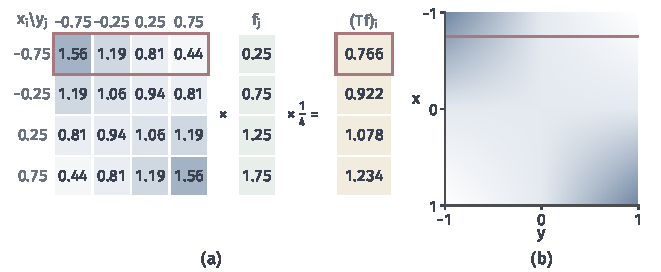
\includegraphics[width=112mm]{figures/04-spaces-measures-and-geometry/03-function-spaces/matplotlib/lop-kernel-as-matrix/figure.pdf}
  \caption{积分算子是矩阵的连续版本，核$k(x,y)=1+xy$就是矩阵元素。(a)四个中点上的矩阵$K_{ij}=1+x_ix_j$，乘以输入$f=1+x$的取值（绿）和格子测度$1/4$，得到输出的近似值（黄）；红框是第一行与它给出的输出。(b)同一个核在连续变量下的取值，纵轴向下对应行号，颜色越深值越大，红线是$x=-3/4$的一行。}
  \label{fig:lop-kernel-as-matrix}
\end{BookInlineFigure}

图中(b)是把格子无限加细后的样子。行变成水平切片，矩阵元素变成曲面上的一点，$k(x,\cdot)$作用于输入的方式与(a)中的第一行相同。

这个对应在哪里失效，也应当说清楚。恒等算子的矩阵是对角线上全为$1$。对角线$\{x=y\}$在正方形中面积为零，任何函数形式的核都承载不了它，所以恒等算子在$L^2(0,1)$上不是积分算子。求导相当于差分矩阵，同样只有对角线附近的元素，也没有函数形式的核。

\paragraph{微分}
在$[0,1]$上令$Df=f^\prime$。连续函数未必可导，例如$f(x)=\lvert x-1/2\rvert$在$x=1/2$处没有导数，所以$D$不能定义在整个$C[0,1]$上。

取定义域$D(D)=C^1[0,1]$，即导数存在且连续的函数，输出$f^\prime\in C[0,1]$，线性来自求导的线性。于是求导是一个从$C[0,1]$到$C[0,1]$、定义在真子空间$C^1[0,1]$上的线性算子。它也可以看成从$C^1[0,1]$到$C[0,1]$的算子，两种看法的区别要到配置范数时才显现出来。

这些例子中，恒等、投影与乘以有界函数自然定义在整个空间上；积分变换须由核与测度的条件保证定义；求导只能定义在一部分函数上。下一节为输入与输出配上范数，研究这些算子是否用一个统一的常数控制误差。

\section{算子范数}
\label{sec:lop-operator-norm}

输入$x$带上扰动$e$以后，线性算子的输出变为$T(x+e)=Tx+Te$。输出误差$Te$只取决于扰动本身，与$x$在哪里无关。于是“误差会被放大多少”化为一个问题：能否找到一个常数，控制一切扰动经过$T$后的大小？

对矩阵，这个问题总有答案。单位球是紧集，$\lVert\bm A\bm x\rVert$连续，最大值一定取到。算子没有这样的保证：单位球不紧，放大倍数可能无穷大。本节先用一个统一不等式定义有界性，再通过求导和积分说明条件的作用，最后定义算子范数。

\subsection{算子的有界性}
\label{sec:lop-boundedness}

下面设$X,Y$是赋范空间，$T:D(T)\to Y$是线性算子，$D(T)\subseteq X$沿用$X$的范数，$Y$使用它自己的范数。我们希望用一个与输入无关的常数$C$控制$\lVert Tx\rVert$，这样输入误差为$\lVert e\rVert$时，输出误差不超过$C\lVert e\rVert$。

\begin{definition}[有界线性算子]
\label{def:lop-bounded-operator}
若存在常数$C\geq0$，使
\begin{equation}
 \lVert Tx\rVert_Y\leq C\lVert x\rVert_X\qquad(x\in D(T)),
 \label{eq:lop-bounded}
\end{equation}
则称线性算子$T$为\term{有界线性算子}（bounded linear operator），简称有界算子。不存在这样的常数时，称$T$为\term{无界算子}（unbounded operator）。
\end{definition}

这里的“有界”说的是输出与输入之比有统一上界，不是说输出集合$\{Tx:x\in D(T)\}$有界：非零线性算子的像在数乘下封闭，总是无界集合。条件~\eqref{eq:lop-bounded}也可以只在单位球上检查。按线性把$x\neq0$缩放为$x/\lVert x\rVert$，它等价于
\[
 \sup\{\lVert Tx\rVert:x\in D(T),\ \lVert x\rVert\leq1\}<\infty.
\]

第~\ref{chap:metric-space-maps}章在度量空间之间定义了连续映射与Lipschitz映射：后者要求存在常数$L$使输出距离不超过$L$倍的输入距离，它比连续更强。对一般映射，二者相差很远；对线性算子，下面的定理说明它们与有界性是一回事。

\begin{theorem}[有界与连续等价]
\label{thm:lop-bounded-continuous}
对赋范空间之间的线性算子$T:D(T)\to Y$，下列四条等价：（i）$T$在$0$处连续；（ii）$T$在$D(T)$上处处连续；（iii）$T$是Lipschitz映射；（iv）$T$有界。
\end{theorem}

\begin{proof}
若（iv）成立，由线性，
\[
 \lVert Tx-Tz\rVert=\lVert T(x-z)\rVert\leq C\lVert x-z\rVert,
\]
这就是（iii）。Lipschitz映射处处连续，故（iii）推出（ii）；处处连续自然包含在$0$处连续，故（ii）推出（i）。

只需再证（i）推出（iv）。取$\varepsilon=1$，由$T$在$0$处连续及$T0=0$，存在$\delta>0$，使$x\in D(T)$且$\lVert x\rVert\leq\delta$时$\lVert Tx\rVert\leq1$。

对任意$x\neq0$，向量$\delta x/\lVert x\rVert$的范数为$\delta$，于是
\[
 \lVert Tx\rVert=\frac{\lVert x\rVert}{\delta}\Bigl\lVert T\Bigl(\frac{\delta x}{\lVert x\rVert}\Bigr)\Bigr\rVert\leq\frac{1}{\delta}\lVert x\rVert .
\]
取$C=1/\delta$即得（iv）。
\end{proof}

证明的关键是缩放：线性算子在零点附近一个小球上的行为，决定了它在所有尺度上的行为。有限维空间中所有范数等价，线性映射总是有界的；无限维中这一点不再自动成立，下面两个例子分别给出失败与成立的情形。

\subsubsection{有界性依赖定义域范数}
\label{sec:lop-derivative-boundedness}

求导的“矩阵”先用差分看清楚。在$[0,1]$上取$n+1$个等距点，步长$h=1/n$，差分$(f_{i+1}-f_i)/h$就是一行只有两个非零元素$\pm1/h$的矩阵。网格加细时，矩阵元素按$1/h$增大。

取输入为交错序列$f_i=(-1)^i$，它的每个分量绝对值都是$1$，输出的每个分量绝对值都是$2/h=2n$。例如$h=1/4$时，输入$(1,-1,1,-1,1)$的输出是$(-8,8,-8,8)$。网格越细，这个矩阵的放大倍数越大，极限下不存在上界。积分的矩阵正好相反，元素里带一个小因子$h$。

现在回到连续的情形。考虑求导$D:C^1[0,1]\to C[0,1]$，$Df=f^\prime$，取值空间始终使用一致范数$\lVert g\rVert_\infty=\max_{[0,1]}\lvert g\rvert$。先在定义域上使用同时计入函数值与导数的范数
\[
 \lVert f\rVert_{C^1}=\lVert f\rVert_\infty+\lVert f^\prime\rVert_\infty .
\]
这时
\[
 \lVert Df\rVert_\infty=\lVert f^\prime\rVert_\infty\leq\lVert f\rVert_{C^1},
\]
取$C=1$即满足式~\eqref{eq:lop-bounded}，$D$是有界算子。

再在同一个函数集合$C^1[0,1]$上只用一致范数衡量输入。取$f_n(x)=\sin(2\pi nx)$，则
\[
 \lVert f_n\rVert_\infty=1,\qquad \lVert Df_n\rVert_\infty=\lVert2\pi n\cos(2\pi nx)\rVert_\infty=2\pi n .
\]
输出与输入的范数之比为$2\pi n$，随$n$无界增长，不存在统一常数，$D$是无界算子。振幅不变而频率升高时，函数值始终在$[-1,1]$中，斜率却按频率放大；一个一致范数很小的高频扰动$\varepsilon f_n$，可以使导数产生$2\pi n\varepsilon$的误差。

两种情形中，求导公式与允许的函数集合都没有变，变化的只是定义域上的范数。所以说一个算子是否有界，必须同时交代作用规则、定义域和两侧的范数。前一种范数把导数的大小也算进输入的“大小”，因而能控制输出；后一种范数看不见导数，也就无从控制它。

两种范数的另一个差别是完备性。只配一致范数的$C^1[0,1]$不是Banach空间。函数$g_n(x)=\sqrt{(x-1/2)^2+n^{-2}}$都连续可导，并且
\[
 0\leq g_n(x)-\lvert x-\tfrac12\rvert=\frac{n^{-2}}{g_n(x)+\lvert x-1/2\rvert}\leq\frac1n,
\]
所以$(g_n)$按一致范数收敛到不可导的$\lvert x-1/2\rvert$，是$C^1[0,1]$中没有极限的柯西列。

第~\ref{sec:lop-fundamental-theorems}节的算子定理都要求Banach空间，因此不能直接套用在这样的定义域上。配上$\lVert\cdot\rVert_{C^1}$后，$C^1[0,1]$是完备的（第~\ref{sec:lop-closed-graph}小节用积分表示说明这一点），那些定理才能使用。

\subsubsection{积分算子的有界性}
\label{sec:lop-integral-bounded}

现在回到积分变换~\eqref{eq:lop-integral-operator}。先看矩阵的情形。输出的第$i$个分量是第$i$行与输入的内积，由Cauchy--Schwarz不等式，它的平方不超过第$i$行的平方和乘以$\lVert\bm f\rVert^2$。

再对$i$求和，就得到
\[
 \lVert\bm K\bm f\rVert^2\leq\Bigl(\sum_{i,j}\lvert K_{ij}\rvert^2\Bigr)\lVert\bm f\rVert^2.
\]
右端括号是矩阵元素的平方和，即Frobenius范数的平方。把求和换成积分，同一个估计给出下面的定理，核的$L^2$范数相当于矩阵的Frobenius范数。

设$(X,\mu)$与$(Y,\nu)$是$\sigma$有限测度空间，固定输入空间$L^2(Y,\nu)$、输出空间$L^2(X,\mu)$，并设核$k\in L^2(X\times Y,\mu\otimes\nu)$。下面用到的乘积测度、Tonelli定理与Fubini定理见第~\ref{chap:integration}章。

\begin{theorem}[平方可积核的有界性]
\label{thm:lop-hs-bounded}
在上述条件下，对每个$f\in L^2(Y,\nu)$，积分~\eqref{eq:lop-integral-operator}对$\mu$几乎每个$x$绝对收敛，所得函数$Tf$可测且属于$L^2(X,\mu)$，并且
\begin{equation}
 \lVert Tf\rVert_{L^2(X,\mu)}\leq\lVert k\rVert_{L^2(X\times Y,\mu\otimes\nu)}\lVert f\rVert_{L^2(Y,\nu)} .
 \label{eq:lop-hs-bound}
\end{equation}
因此$T:L^2(Y,\nu)\to L^2(X,\mu)$是有界线性算子。
\end{theorem}

\begin{proof}
第一步，取得平方可积的截面。对非负可测函数$\lvert k\rvert^2$用Tonelli定理，
\[
 \int_X\Bigl(\int_Y\lvert k(x,y)\rvert^2\,\mathrm d\nu(y)\Bigr)\mathrm d\mu(x)=\lVert k\rVert_{L^2(\mu\otimes\nu)}^2<\infty ,
\]
所以内层积分对$\mu$几乎每个$x$有限，即截面$k(x,\cdot)\in L^2(Y,\nu)$对几乎每个$x$成立。

第二步，逐点估计。对这样的$x$，由Cauchy--Schwarz不等式，
\[
 \int_Y\lvert k(x,y)f(y)\rvert\,\mathrm d\nu(y)\leq\lVert k(x,\cdot)\rVert_{L^2(\nu)}\lVert f\rVert_{L^2(\nu)}<\infty ,
\]
积分绝对收敛，并且
\[
 \lvert(Tf)(x)\rvert\leq\lVert k(x,\cdot)\rVert_{L^2(\nu)}\lVert f\rVert_{L^2(\nu)}.
\]
在例外的零测集上令$Tf=0$。

第三步，核对可测性。取$\mu(E)<\infty$的可测集$E\subseteq X$，对第二步的逐点界关于$x\in E$积分，再用一次Cauchy--Schwarz不等式，
\[
 \int_E\int_Y\lvert k(x,y)f(y)\rvert\,\mathrm d\nu(y)\,\mathrm d\mu(x)
 \leq\mu(E)^{1/2}\lVert k\rVert_{L^2(\mu\otimes\nu)}\lVert f\rVert_{L^2(\nu)}<\infty .
\]
所以$(x,y)\mapsto k(x,y)f(y)$在$E\times Y$上可积，由Fubini定理，内层积分$x\mapsto(Tf)(x)$在$E$上可测。$X$是可数个有限测度集合之并，故$Tf$在$X$上可测。

第四步，对$x$积分。把第二步的逐点界平方后积分，再用第一步的等式，
\[
 \begin{aligned}
 \lVert Tf\rVert_{L^2(\mu)}^2
 &\leq\int_X\lVert k(x,\cdot)\rVert_{L^2(\nu)}^2\,\mathrm d\mu(x)\,\lVert f\rVert_{L^2(\nu)}^2\\
 &=\lVert k\rVert_{L^2(\mu\otimes\nu)}^2\lVert f\rVert_{L^2(\nu)}^2 .
 \end{aligned}
\]

最后，若$f=g$几乎处处，两者的积分对每个允许的$x$相同，所以$T$作用在等价类上是确定的；线性来自积分的线性。
\end{proof}

平方可积核给出的积分算子称为\term{Hilbert--Schmidt积分算子}（Hilbert--Schmidt integral operator）。证明中的每一步都依赖所选的空间：核平方可积保证截面平方可积，输入属于$L^2(\nu)$才能与截面配对，输出的估计又是按$L^2(\mu)$范数给出的。同一个核公式换成别的输入空间，就要重新核对。

平方可积只是充分条件。取$X=Y=\mathbb N$并配计数测度，$L^2$就是$\ell^2$，积分就是求和，核就是真正的无穷矩阵。单位矩阵$k(m,n)=1$（$m=n$）、$k(m,n)=0$（$m\neq n$）给出恒等算子，它有界；但$\sum_{m,n}\lvert k(m,n)\rvert^2$是无穷多个$1$之和，发散。

\subsection{算子范数的定义}
\label{sec:lop-norm-definition}

有界性只说常数$C$存在，不同的$C$都可以满足式~\eqref{eq:lop-bounded}。为了比较不同算子放大误差的程度，我们取能够使用的最小常数。这正是矩阵的最大放大倍数在算子上的对应物。

\begin{definition}[算子范数]
\label{def:lop-operator-norm}
设$T:D(T)\to Y$是有界线性算子。称
\begin{equation}
 \lVert T\rVert=\sup\{\lVert Tx\rVert_Y:x\in D(T),\ \lVert x\rVert_X\leq1\}
 \label{eq:lop-operator-norm}
\end{equation}
为$T$的\term{算子范数}（operator norm）。
\end{definition}

\begin{theorem}[算子范数是最小的误差常数]
\label{thm:lop-norm-minimal}
设$T$有界。则对一切$x\in D(T)$，
\begin{equation}
 \lVert Tx\rVert\leq\lVert T\rVert\,\lVert x\rVert,
 \label{eq:lop-norm-inequality}
\end{equation}
并且若常数$C\geq0$满足式~\eqref{eq:lop-bounded}，则$\lVert T\rVert\leq C$。因此$\lVert T\rVert$是式~\eqref{eq:lop-bounded}中可取的最小非负常数。
\end{theorem}

\begin{proof}
对$x\neq0$，$x/\lVert x\rVert$属于单位球，由定义它的输出范数不超过$\lVert T\rVert$，乘回$\lVert x\rVert$即得第一式；$x=0$时两边都为零。

反过来，若$C$满足式~\eqref{eq:lop-bounded}，则对单位球中的每个$x$有$\lVert Tx\rVert\leq C\lVert x\rVert\leq C$，对$x$取上确界得$\lVert T\rVert\leq C$。
\end{proof}

对两个输入之差用式~\eqref{eq:lop-norm-inequality}，再由线性，得到
\begin{equation}
 \lVert Tx-Tz\rVert\leq\lVert T\rVert\,\lVert x-z\rVert\qquad(x,z\in D(T)).
 \label{eq:lop-lipschitz}
\end{equation}
所以算子范数统一控制输入差造成的输出差：无论输入落在哪里，误差至多被放大$\lVert T\rVert$倍，而且没有更小的常数对全部输入都有效。

\paragraph{求导的算子范数}
对配$\lVert\cdot\rVert_{C^1}$的求导，上一小节已得$\lVert D\rVert\leq1$。取$f_n(x)=\sin(2\pi nx)/(2\pi n)$，有
\[
 \lVert Df_n\rVert_\infty=1,\qquad\lVert f_n\rVert_{C^1}=1+\frac1{2\pi n},
\]
比值趋于$1$，所以$\lVert D\rVert=1$。这个上确界不被任何输入取到：$\lVert Df\rVert_\infty=\lVert f\rVert_{C^1}$要求$\lVert f\rVert_\infty=0$。因此算子范数应理解为最小的统一上界，不能无条件称为“最大输出”。

\paragraph{积分算子的两个范数}
对平方可积核，定理~\ref{thm:lop-hs-bounded}与定理~\ref{thm:lop-norm-minimal}合起来给出
\begin{equation}
 \lVert T\rVert\leq\lVert k\rVert_{L^2(X\times Y,\mu\otimes\nu)} .
 \label{eq:lop-hs-norm}
\end{equation}
左边相当于矩阵的最大放大倍数，右边相当于矩阵元素的平方和开根。矩阵论中这两个数一般不相等，下面用贯穿例子把两个数都算出来。

先算核的$L^2$范数。在例子~\eqref{eq:lop-running-kernel}中，$\int x\,\mathrm d\mu=0$，$\int x^2\,\mathrm d\mu=1/3$，所以
\[
 \lVert k\rVert_{L^2(\mu\otimes\mu)}^2=\iint(1+xz)^2\,\mathrm d\mu(x)\,\mathrm d\mu(z)=1+2\cdot0+\frac13\cdot\frac13=\frac{10}{9}.
\]

算子范数可以直接算出。函数$e_1=1$与$e_2=\sqrt3x$在$L^2(\mu)$中标准正交，因为$\int3x^2\,\mathrm d\mu=1$。式~\eqref{eq:lop-running-kernel}可写成
\[
 Tf=\langle e_1,f\rangle e_1+\frac13\langle e_2,f\rangle e_2.
\]
在坐标$(\langle e_1,f\rangle,\langle e_2,f\rangle)$下，$T$相当于对角矩阵$\operatorname{diag}(1,1/3)$，其余方向全部被送到零。

由勾股定理和Bessel不等式，
\[
 \lVert Tf\rVert^2=\lvert\langle e_1,f\rangle\rvert^2+\frac19\lvert\langle e_2,f\rangle\rvert^2\leq\lvert\langle e_1,f\rangle\rvert^2+\lvert\langle e_2,f\rangle\rvert^2\leq\lVert f\rVert^2 .
\]
取$f=e_1=1$时等号成立，所以$\lVert T\rVert=1$，严格小于$\sqrt{10/9}=\sqrt{10}/3$。核的$L^2$范数只是算子范数的上界，二者一般不相等。

图~\ref{fig:lop-norm-ellipse}画出这件事。单位圆被压成半轴为$1$与$1/3$的椭圆，最长半轴就是算子范数。$f=1+x$的放大倍数可以直接算出。由$\lVert e_2\rVert=1$及$f=e_1+e_2/\sqrt3$，得到
\[
 \lVert f\rVert^2=1+\frac13=\frac43,\qquad\lVert Tf\rVert^2=1+\frac19\cdot\frac13=\frac{28}{27}.
\]
两式相除，放大倍数是
\[
 \frac{\lVert Tf\rVert}{\lVert f\rVert}=\sqrt{\frac{28}{27}\cdot\frac34}=\frac{\sqrt7}3\approx0.882.
\]

\begin{BookInlineFigure}
  \centering
  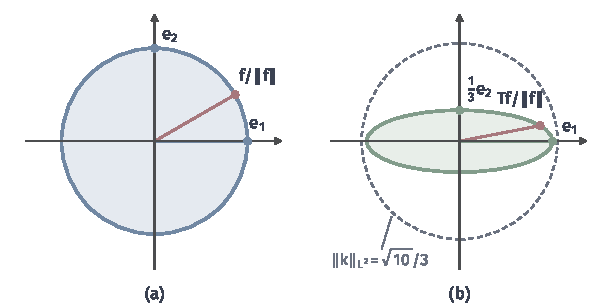
\includegraphics[width=104mm]{figures/04-spaces-measures-and-geometry/03-function-spaces/matplotlib/lop-norm-ellipse/figure.pdf}
  \caption{贯穿例子在$\operatorname{span}\{e_1,e_2\}$上的放大倍数。(a)输入坐标$(\langle e_1,f\rangle,\langle e_2,f\rangle)$中的单位圆（蓝），红点是归一化的$f=1+x$。(b)输出的椭圆（绿），半轴$1$与$1/3$，最长半轴等于$\lVert T\rVert=1$；虚线圆的半径是核的$L^2$范数$\sqrt{10}/3$，它只是上界。}
  \label{fig:lop-norm-ellipse}
\end{BookInlineFigure}

\paragraph{有界算子的矩阵}
到目前为止，矩阵只是类比。在可分Hilbert空间中，有界性让这个类比成为等式。设$H$有标准正交基$(e_n)_{n\geq1}$，$T\in\mathcal B(H)$（记号见下一小节），规定矩阵元素
\begin{equation}
 A_{mn}=\langle e_m,Te_n\rangle .
 \label{eq:lop-matrix-entry}
\end{equation}

任取$x=\sum_nx_ne_n$，部分和$\sum_{n\leq N}x_ne_n$按范数收敛到$x$。由$T$连续，
\[
 Tx=\lim_{N\to\infty}\sum_{n\leq N}x_nTe_n.
\]
再用内积对第二个变量连续，读出第$m$个坐标，就得到矩阵乘法公式
\[
 \langle e_m,Tx\rangle=\sum_nA_{mn}x_n .
\]
连续性在这里不可缺少：它保证算子由基向量上的取值决定。

两个矩阵后面会反复用到。对角算子$A(x_n)=(x_n/n)$在$\ell^2$上的矩阵是$\operatorname{diag}(1,1/2,1/3,\ldots)$；由$\lVert Ax\rVert\leq\lVert x\rVert$及$Ae_1=e_1$得$\lVert A\rVert=1$。右移$S(x_1,x_2,\ldots)=(0,x_1,x_2,\ldots)$的矩阵只在紧贴主对角线下方的一条斜线上为$1$，它保持长度，所以$\lVert S\rVert=1$。

反过来，并非每个无穷矩阵都给出有界算子。对角矩阵$\operatorname{diag}(1,2,3,\ldots)$的放大倍数无界，这是有限维中没有的现象。

\subsection{算子范数的性质}
\label{sec:lop-norm-properties}

同一对空间之间的算子可以相加和数乘：对$S,T:X\to Y$及标量$\alpha$，令$(S+T)x=Sx+Tx$，$(\alpha T)x=\alpha Tx$。若$T:X\to Y$、$S:Y\to Z$，前者的取值空间正是后者的输入空间，就可以复合，$(S\circ T)x=S(Tx)$，常简写为$ST$，先作用$T$、再作用$S$，这对应矩阵乘法。

这些运算都保持线性；下面说明它们也保持有界，并给出范数怎样变化。记$\mathcal B(X,Y)$为定义在整个$X$上、取值于$Y$的有界线性算子全体，$X=Y$时简记$\mathcal B(X)$。

\begin{theorem}[算子范数的基本性质]
\label{thm:lop-norm-properties}
设$X,Y,Z$是赋范空间，$S,T\in\mathcal B(X,Y)$，$R\in\mathcal B(Y,Z)$，$\alpha\in\mathbb F$。则
$\lVert T\rVert\geq0$，且$\lVert T\rVert=0$当且仅当$T=0$；$RT\in\mathcal B(X,Z)$；并且
\begin{equation}
 \begin{gathered}
 \lVert\alpha T\rVert=\lvert\alpha\rvert\,\lVert T\rVert,\qquad
 \lVert S+T\rVert\leq\lVert S\rVert+\lVert T\rVert,\\
 \lVert RT\rVert\leq\lVert R\rVert\,\lVert T\rVert.
 \end{gathered}
 \label{eq:lop-norm-properties}
\end{equation}
因此$\mathcal B(X,Y)$在算子范数下是赋范空间。
\end{theorem}

\begin{proof}
几个估计都先对单个输入成立，再对单位球取上确界。先看正定性。若$\lVert T\rVert=0$，由定理~\ref{thm:lop-norm-minimal}，$\lVert Tx\rVert\leq0$对一切$x$成立，即$T=0$。反之$T=0$时单位球的输出全为零。

数乘由$Y$中范数的齐次性得到：
\[
 \lVert\alpha Tx\rVert=\lvert\alpha\rvert\,\lVert Tx\rVert,
\]
取上确界即得。

加法用$Y$中的三角不等式。对$\lVert x\rVert\leq1$，
\[
 \lVert(S+T)x\rVert\leq\lVert Sx\rVert+\lVert Tx\rVert\leq\lVert S\rVert+\lVert T\rVert.
\]

复合时先用$R$的估计，再用$T$的估计：
\[
 \lVert R(Tx)\rVert_Z\leq\lVert R\rVert\,\lVert Tx\rVert_Y\leq\lVert R\rVert\,\lVert T\rVert\,\lVert x\rVert_X.
\]
这里$Tx$用$Y$的范数衡量，它正是$R$的算子范数所用的输入范数；若$R$的输入范数换成$Y$上的另一个范数，这一步就不能直接衔接。
\end{proof}

复合估计给出多步变换的统一误差上界：输入误差经过$T$至多放大$\lVert T\rVert$倍，再经过$R$至多再放大$\lVert R\rVert$倍。这个上界一般不是等式。在平面上取$\bm T=\operatorname{diag}(1,0)$、$\bm R=\operatorname{diag}(0,1)$，两者的范数都是$1$，乘积却是零矩阵：$\bm T$保留的方向恰好被$\bm R$消去。

\paragraph{算子空间的完备性}
后面要用有限秩算子的极限构造紧算子，对算子级数求和，这需要算子列的极限仍然留在$\mathcal B(X,Y)$中。下面的结论说明，只要取值空间完备，这一点就成立。

\begin{theorem}[算子空间的完备性]
\label{thm:lop-operator-space-complete}
设$X$是赋范空间，$Y$是Banach空间。则$\mathcal B(X,Y)$在算子范数下是Banach空间。
\end{theorem}

\begin{proof}
设$(T_n)$是$\mathcal B(X,Y)$中的柯西列。对固定的$x\in X$，
\[
 \lVert T_nx-T_mx\rVert\leq\lVert T_n-T_m\rVert\,\lVert x\rVert,
\]
所以$(T_nx)$是$Y$中的柯西列。$Y$完备，极限存在，记为$Tx$。由极限的线性，$T$是线性的。

给定$\varepsilon>0$，取$N$使$n,m\geq N$时$\lVert T_n-T_m\rVert<\varepsilon$。对任意$\lVert x\rVert\leq1$及$n\geq N$，有$\lVert T_nx-T_mx\rVert<\varepsilon$。固定$n$而令$m\to\infty$，得
\[
 \lVert T_nx-Tx\rVert\leq\varepsilon\qquad(\lVert x\rVert\leq1,\ n\geq N).
\]

于是$\lVert Tx\rVert\leq\lVert T_N\rVert+\varepsilon$对单位球中的$x$成立，$T$有界。同一估计又说明$\lVert T_n-T\rVert\leq\varepsilon$（$n\geq N$），即$T_n\to T$按算子范数收敛。
\end{proof}

证明只用到了$Y$的完备性，输入空间$X$不必完备。一个直接的用途是：若$T_j\in\mathcal B(X,Y)$且$\sum_j\lVert T_j\rVert<\infty$，则部分和满足
\[
 \Bigl\lVert\sum_{j=m+1}^nT_j\Bigr\rVert\leq\sum_{j=m+1}^n\lVert T_j\rVert,
\]
是柯西列，因而级数$\sum_jT_j$按算子范数收敛。第~\ref{chap:operator-spectra}章用它说明谱的有界性，第~\ref{chap:linear-operator-equations}章再用它构造逆算子。

\section{包含映射}
\label{sec:lop-inclusions}

一个函数可以同时属于几个函数空间，并在各自的范数下得到不同的“大小”。若我们在一个空间的范数下估计了误差，常常还想知道它在另一个范数下有多大。例如数值方法给出了$L^2$误差，能否推出$L^1$误差也小？

用矩阵的语言说，输入和输出是同一个向量，算子是单位矩阵，只是两边用的尺子不同。第~\ref{sec:lop-operator-norm}节的算子范数正好衡量这两把尺子的比例。

设$X,Y$是赋范空间，且$X\subseteq Y$作为线性空间成立。映射$\iota:X\to Y$，$\iota x=x$称为\term{包含映射}（inclusion map）。它把元素原样送出，因而线性。若它有界，即存在$C$使
\begin{equation}
 \lVert x\rVert_Y\leq C\lVert x\rVert_X\qquad(x\in X),
 \label{eq:lop-embedding}
\end{equation}
就称$X$\term{连续嵌入}（continuous embedding）$Y$。这时$X$中的误差估计自动转为$Y$中的误差估计，常数$C$就是$\lVert\iota\rVert$的上界。

集合包含、连续嵌入与范数等价是三个逐步加强的要求。集合包含只说元素可以对应过去。连续嵌入还要求一个方向的范数控制。若$X$与$Y$是同一个线性空间，且两个方向都有控制
\[
 c\lVert x\rVert_X\leq\lVert x\rVert_Y\leq C\lVert x\rVert_X,
\]
两个范数等价，它们给出同样的收敛与同样的开集。

有限维中三者没有区别，因为所有范数都等价。无限维中集合包含不保证连续嵌入。在$C[0,1]$上取两个范数$\lVert f\rVert_1=\int_0^1\lvert f\rvert$与$\lVert f\rVert_\infty$，两者作用于同一个函数集合。

令$f_n$是以$0$为顶点、高为$1$、底为$[0,2/n]$的三角形函数，它的面积与高度分别是
\[
 \lVert f_n\rVert_1=\frac1n,\qquad\lVert f_n\rVert_\infty=1.
\]
比值$\lVert f_n\rVert_\infty/\lVert f_n\rVert_1=n$无界，所以从$(C[0,1],\lVert\cdot\rVert_1)$到$(C[0,1],\lVert\cdot\rVert_\infty)$的恒等映射无界。反方向$\lVert f\rVert_1\leq\lVert f\rVert_\infty$成立，所以只有一个方向的连续嵌入，两个范数不等价。

\subsection{Lᵖ空间的包含}
\label{sec:lop-lp-inclusion}

在有限测度空间上，大指数的$L^q$范数能控制小指数的$L^p$范数。直观上，$\lvert f\rvert^q$比$\lvert f\rvert^p$更重地惩罚大的取值；测度有限又排除了“取值很小却铺满无穷大区域”的情形，所以小指数范数不会比大指数范数大很多。

\begin{theorem}[有限测度上的Lᵖ包含]
\label{thm:lop-lp-inclusion}
设$(\Omega,\mathcal F,\mu)$是测度空间，$\mu(\Omega)<\infty$，$1\leq p\leq q\leq\infty$。则$L^q(\mu)\subseteq L^p(\mu)$，并且
\begin{equation}
 \lVert f\rVert_p\leq\mu(\Omega)^{1/p-1/q}\lVert f\rVert_q\qquad(f\in L^q(\mu)),
 \label{eq:lop-lp-inclusion}
\end{equation}
其中$q=\infty$时约定$1/q=0$。因此包含映射$\iota:L^q(\mu)\to L^p(\mu)$有界，$\lVert\iota\rVert\leq\mu(\Omega)^{1/p-1/q}$；$\mu(\Omega)>0$时等号成立。
\end{theorem}

\begin{proof}
$p=q$时结论就是$\lVert f\rVert_p\leq\lVert f\rVert_p$。设$q=\infty$，$p<\infty$，则$\lvert f\rvert\leq\lVert f\rVert_\infty$几乎处处，于是
\[
 \int\lvert f\rvert^p\,\mathrm d\mu\leq\lVert f\rVert_\infty^p\,\mu(\Omega),
\]
开$p$次方即得。

设$p<q<\infty$。令$r=q/p>1$，其共轭指数为$r^\prime=q/(q-p)$。对$\lvert f\rvert^p$与常函数$1$用Hölder不等式，
\[
 \int\lvert f\rvert^p\cdot1\,\mathrm d\mu
 \leq\Bigl(\int\lvert f\rvert^{pr}\,\mathrm d\mu\Bigr)^{1/r}\Bigl(\int1\,\mathrm d\mu\Bigr)^{1/r^\prime}.
\]
右端第一个因子的$pr=q$，第二个因子的$1/r^\prime=1-p/q$，所以
\[
 \int\lvert f\rvert^p\,\mathrm d\mu\leq\lVert f\rVert_q^p\,\mu(\Omega)^{1-p/q}.
\]
开$p$次方得式~\eqref{eq:lop-lp-inclusion}。

两个空间中的元素都是同一测度下的几乎处处等价类，所以$\iota$把一个等价类送到它自己，是单射。最后，$f=1$属于$L^q$，范数分别为$\lVert1\rVert_p=\mu(\Omega)^{1/p}$与$\lVert1\rVert_q=\mu(\Omega)^{1/q}$，比值恰为$\mu(\Omega)^{1/p-1/q}$，所以范数估计不能改进。
\end{proof}

对概率测度，$\mu(\Omega)=1$，式~\eqref{eq:lop-lp-inclusion}说明$\lVert f\rVert_p$随$p$单调不减。例如在$[0,1]$上取$f(x)=x$，依次得到
\[
 \lVert f\rVert_1=\frac12,\qquad\lVert f\rVert_2=\frac1{\sqrt3}\approx0.577,\qquad\lVert f\rVert_\infty=1.
\]
一般地，$\lVert x\rVert_p=(p+1)^{-1/p}$，图~\ref{fig:lop-lp-inclusion}(a)中蓝色曲线就是它。

\paragraph{无限测度上的失败}
有限测度条件不能去掉。在$(0,\infty)$上取Lebesgue测度，函数$f(x)=x^{-1}\mathbf 1_{\{x\geq1\}}$满足
\[
 \int_1^\infty x^{-2}\,\mathrm dx=1,\qquad\int_1^\infty x^{-1}\,\mathrm dx=\infty,
\]
所以它属于$L^2$而不属于$L^1$：慢慢衰减的尾部在小指数下累积出无穷的总量。

反过来，$g(x)=x^{-1/2}\mathbf 1_{\{0<x<1\}}$满足
\[
 \int_0^1x^{-1/2}\,\mathrm dx=2,\qquad\int_0^1x^{-1}\,\mathrm dx=\infty,
\]
所以它属于$L^1$而不属于$L^2$：靠近原点的尖峰在大指数下被放大。在这里两个方向的包含都不成立，图~\ref{fig:lop-lp-inclusion}(b)画出了这两种失败的来源。

计数测度给出另一种情形。在$\mathbb N$上，若$\lVert a\rVert_p\leq1$，则每个$\lvert a_n\rvert\leq1$，于是$\lvert a_n\rvert^q\leq\lvert a_n\rvert^p$。求和得$\lVert a\rVert_q\leq1$，按齐次性，
\[
 \lVert a\rVert_q\leq\lVert a\rVert_p\qquad(p\leq q).
\]

包含方向恰好反过来：$\ell^p\subseteq\ell^q$。每个点的测度为$1$，排除了尖峰，却允许无穷多个点。图~\ref{fig:lop-lp-inclusion}(a)中绿色曲线是有限序列$(1,1/2,1/3)$的$\ell^p$范数，随$p$下降。指数方向由测度的结构决定，不能把有限测度上的包含照搬到任意测度空间。

\begin{BookInlineFigure}
  \centering
  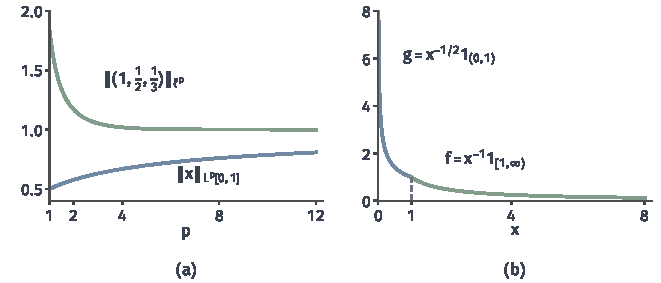
\includegraphics[width=112mm]{figures/04-spaces-measures-and-geometry/03-function-spaces/matplotlib/lop-lp-inclusion/figure.pdf}
  \caption{$L^p$范数随指数变化的方向由测度决定。(a)概率测度上$\lVert x\rVert_{L^p[0,1]}=(p+1)^{-1/p}$随$p$增大（蓝），计数测度上$(1,1/2,1/3)$的$\ell^p$范数随$p$减小（绿）。(b)$(0,\infty)$上两种失败：尖峰$g=x^{-1/2}\mathbf 1_{(0,1)}$在$L^1\setminus L^2$中（蓝），长尾$f=x^{-1}\mathbf 1_{[1,\infty)}$在$L^2\setminus L^1$中（绿）。}
  \label{fig:lop-lp-inclusion}
\end{BookInlineFigure}

\subsection{改变测度后的范数比较}
\label{sec:lop-change-of-measure}

在同一个可测空间上换一个测度，函数的$L^p$范数就要用新测度计算。设$h\geq0$可测，$\nu$由$\mathrm d\nu=h\,\mathrm d\mu$给出，即$\nu(E)=\int_Eh\,\mathrm d\mu$；第~\ref{chap:measure-densities}章把$h$称为$\nu$关于$\mu$的密度。

按向量的类比，这相当于给每个分量换一个权重$h(x)$。我们想知道$L^p(\mu)$中的误差能否控制$L^p(\nu)$中的误差，下面设$1\leq p<\infty$。

\paragraph{等价类的对应}
比较之前先要说明映射本身有意义。$L^p(\mu)$的元素是$\mu$几乎处处相等的等价类，$L^p(\nu)$的元素是$\nu$几乎处处相等的等价类。

若$f=g$在$\mu$几乎处处成立，记$N=\{f\neq g\}$，则$\mu(N)=0$，从而
\[
 \nu(N)=\int_Nh\,\mathrm d\mu=0.
\]
所以$\mu$等价类中的函数在$\nu$下也属于同一个等价类，映射$J[f]_\mu=[f]_\nu$不依赖代表的选取。这一步用的正是$\nu$关于$\mu$绝对连续：$\mu$零测集也是$\nu$零测集。

\begin{theorem}[有界密度给出有界映射]
\label{thm:lop-change-of-measure}
设$\mathrm d\nu=h\,\mathrm d\mu$，且存在常数$C$使$h\leq C$在$\mu$几乎处处成立。则对$f\in L^p(\mu)$有$f\in L^p(\nu)$，并且
\begin{equation}
 \lVert f\rVert_{L^p(\nu)}\leq C^{1/p}\lVert f\rVert_{L^p(\mu)} .
 \label{eq:lop-change-of-measure}
\end{equation}
所以$J:L^p(\mu)\to L^p(\nu)$是有界线性映射，$\lVert J\rVert\leq C^{1/p}$。
\end{theorem}

\begin{proof}
对非负可测函数$\lvert f\rvert^p$，由密度的定义，
\[
 \int\lvert f\rvert^p\,\mathrm d\nu=\int\lvert f\rvert^ph\,\mathrm d\mu\leq C\int\lvert f\rvert^p\,\mathrm d\mu.
\]
开$p$次方即得。线性由$J$在代表上作恒等变换得到。
\end{proof}

\paragraph{映射可能不是单射}
权重为零的分量不再被计入，所以$J$不一定区分$L^p(\mu)$中不同的元素。若$h=0$在某个满足$0<\mu(A)<\infty$的集合$A$上成立，则$\mathbf 1_A$在$L^p(\mu)$中非零，但
\[
 \int\mathbf 1_A\,\mathrm d\nu=\int_Ah\,\mathrm d\mu=0,
\]
所以$J\mathbf 1_A=0$。新测度看不见$A$上发生的事情，$\ker J$由在$\{h>0\}$上几乎处处为零的函数组成。

若$h>0$在$\mu$几乎处处成立，两种零测集就一致。一方面，绝对连续已给出由$\mu(E)=0$推出$\nu(E)=0$。另一方面，若$\nu(E)=\int_Eh\,\mathrm d\mu=0$，则$h\mathbf 1_E=0$在$\mu$几乎处处成立，而$h>0$几乎处处，只能$\mathbf 1_E=0$几乎处处，即$\mu(E)=0$。

这时两种等价类相同，$J$是单射；但$h$可以任意接近零，$J$仍可能不满射，逆映射也可能无界。在$[0,1]$上取$h(x)=x$，函数$x^{-3/4}$满足$\int x^{-3/2}\cdot x\,\mathrm dx<\infty$，属于$L^2(\nu)$，而$\int x^{-3/2}\,\mathrm dx=\infty$，不属于$L^2(\mu)$，所以$J$不是满射。

若密度还有正下界，即$0<c\leq h\leq C$几乎处处，同样的计算给出
\begin{equation}
 c^{1/p}\lVert f\rVert_{L^p(\mu)}\leq\lVert f\rVert_{L^p(\nu)}\leq C^{1/p}\lVert f\rVert_{L^p(\mu)} .
 \label{eq:lop-measure-equivalence}
\end{equation}
这时$L^p(\mu)$与$L^p(\nu)$是同一个函数空间，两个范数等价。例如在$[0,1]$上取$h(x)=1+x$，有$1\leq h\leq2$，两个$L^2$范数之比始终在$1$与$\sqrt2$之间。

若取$h(x)=x$，下界消失。令$f_n=\sqrt n\,\mathbf 1_{(0,1/n)}$，则$\lVert f_n\rVert_{L^2(\mu)}=1$，而
\[
 \lVert f_n\rVert_{L^2(\nu)}^2=n\int_0^{1/n}x\,\mathrm dx=\frac1{2n}\to0.
\]
反方向的控制不存在。权重越接近零的区域，越能藏住$\mu$意义下的大函数。

\section{算子列的收敛}
\label{sec:lop-operator-convergence}

实际计算中，我们常用一列逐渐精细的近似算子$T_n$代替一个算子$T$，例如只保留前$n$个展开系数，或者把积分区域截去一小块。对手中的每个输入，近似输出会越来越准；但这是否意味着存在一个只依赖$n$的误差界，对所有单位输入同时有效？

有限维中这不成问题：矩阵的每个元素收敛，整个矩阵就按任何范数收敛。无限维中矩阵有无穷多列，“每一列都收敛”和“所有列一起收敛”不再是一回事，这两种要求的量词次序不同，强弱也不同。

\begin{definition}[算子范数收敛与强算子收敛]
\label{def:lop-operator-convergence}
设$X,Y$是赋范空间，$T_n,T\in\mathcal B(X,Y)$。若
\begin{equation}
 \lVert T_n-T\rVert\to0,
 \label{eq:lop-norm-convergence}
\end{equation}
则称$T_n$\term{算子范数收敛}（convergence in operator norm）到$T$。若
\begin{equation}
 \lVert T_nx-Tx\rVert_Y\to0\qquad(\text{对每个}x\in X),
 \label{eq:lop-strong-convergence}
\end{equation}
则称$T_n$\term{强算子收敛}（strong operator convergence）到$T$。
\end{definition}

算子范数收敛给出统一误差：$\lVert T_n-T\rVert$只依赖$n$，对单位球中的全部输入同时控制输出误差。强算子收敛给出逐输入误差：先固定$x$，再让$n\to\infty$，收敛快慢可以随$x$变化。由
\[
 \lVert T_nx-Tx\rVert\leq\lVert T_n-T\rVert\,\lVert x\rVert,
\]
算子范数收敛蕴含强算子收敛；下面的例子说明反过来不成立。

强算子收敛中的“逐点”，指的是对每个输入向量$x$，像向量$T_nx$在$Y$的范数下收敛。当$X,Y$是函数空间时，它不是说函数$T_nx$在定义域的每个点处收敛，后者是函数列的另一种收敛方式，二者不能混用。

\paragraph{截断投影}
设$H$是无限维可分Hilbert空间，$(e_k)_{k\geq1}$是标准正交基，$P_n$是到$\operatorname{span}\{e_1,\ldots,e_n\}$的正交投影，即
\[
 P_nx=\sum_{k\leq n}\langle e_k,x\rangle e_k.
\]
按第~\ref{sec:lop-norm-definition}小节的矩阵表示，$P_n$是对角矩阵$\operatorname{diag}(1,\ldots,1,0,0,\ldots)$，前$n$个对角元素为$1$。

固定$x$。由第~\ref{chap:function-inner-product-spaces}章的Parseval等式，
\[
 \lVert x-P_nx\rVert^2=\sum_{k>n}\lvert\langle e_k,x\rangle\rvert^2\to0,
\]
因为右端是一个收敛级数的尾部，这个级数的和是$\lVert x\rVert^2$。所以$P_n$强算子收敛到恒等算子$I$。

另一方面，对每个$n$，被截掉的单位向量$e_{n+1}$满足$P_ne_{n+1}=0$，于是
\[
 \lVert(I-P_n)e_{n+1}\rVert=1.
\]
又$I-P_n$是到正交补的投影，$\lVert I-P_n\rVert\leq1$。所以$\lVert I-P_n\rVert=1$对一切$n$成立，$P_n$不按算子范数收敛到$I$。在矩阵上看，差$I-P_n$是$\operatorname{diag}(0,\ldots,0,1,1,\ldots)$，对角线上总还有$1$。

图~\ref{fig:lop-projection-strong-norm}比较了三个输入的截断误差。系数为$2^{-k/2}$的单位向量，其截断误差为$2^{-n/2}$，衰减很快；系数与$1/k$成比例的单位向量衰减慢得多。

\begin{BookInlineFigure}
  \centering
  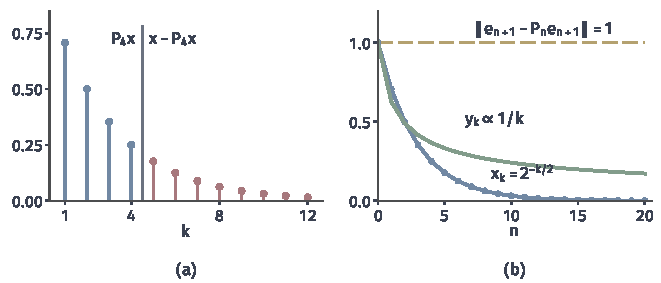
\includegraphics[width=112mm]{figures/04-spaces-measures-and-geometry/03-function-spaces/matplotlib/lop-projection-strong-norm/figure.pdf}
  \caption{截断投影的强收敛与算子范数不收敛。(a)单位向量$x$的系数$c_k=2^{-k/2}$，$P_4$保留蓝色的前四项，红色尾项构成误差$x-P_4x$。(b)截断误差随保留项数$n$的变化：$\lVert x-P_nx\rVert=2^{-n/2}$（蓝），系数与$1/k$成比例的单位向量$y$（绿）衰减较慢，而被截掉的基向量$e_{n+1}$的误差始终为$1$（黄虚线）。}
  \label{fig:lop-projection-strong-norm}
\end{BookInlineFigure}

每个固定输入的误差都趋于零，但不同输入的速度可以任意慢，而被截掉的那个基向量的误差始终是$1$。“每个元素都能被有限维子空间逼近”并不意味着同一个有限维子空间能以任意精度统一逼近整个单位球。

\paragraph{有限个输入上的统一控制}
强算子收敛对有限个输入仍可同时控制。设$x^{(1)},\ldots,x^{(m)}$是固定的输入，对每个$i$取$N_i$使误差小于$\varepsilon$，再取$N=\max_iN_i$即可。

截断投影失去统一控制的原因是单位球中有无穷多个相互正交的方向，每个$P_n$只能照顾其中有限个。第~\ref{sec:lop-uniform-boundedness}小节将说明，在Banach空间上，强算子收敛的算子列至少有统一的范数上界。

\paragraph{函数空间中的截断}
在$L^2(0,1)$中，按二分区间依次排列
\[
 I_1=[0,1],\quad I_2=[0,\tfrac12],\quad I_3=[\tfrac12,1],\quad I_4=[0,\tfrac14],\ \ldots,
\]
长度$\lvert I_n\rvert\to0$。令$T_nf=(1-\mathbf 1_{I_n})f$，即把输入在$I_n$上的部分抹去，这是一个乘法算子。对每个$f\in L^2$，
\[
 \lVert f-T_nf\rVert_2^2=\int_{I_n}\lvert f\rvert^2\,\mathrm dx\to0,
\]
因为$\lvert f\rvert^2$可积，积分区域的测度趋于零时积分趋于零。所以$T_n$强算子收敛到$I$。

同一列算子却不按算子范数收敛。取$f_n=\lvert I_n\rvert^{-1/2}\mathbf 1_{I_n}$，它是单位向量且$(I-T_n)f_n=f_n$，故$\lVert I-T_n\rVert=1$。

更值得注意的是，取$f=1$，每个$x\in[0,1]$都落在无穷多个$I_n$中，也落在无穷多个$I_n$之外。于是$(T_nf)(x)$在$0$与$1$之间无穷次跳动，对任何$x$都不收敛。强算子收敛成立，输出函数却在每一点都不收敛，这正说明二者是不同的概念。

\section{伴随算子}
\label{sec:lop-adjoint}

矩阵有共轭转置，它在算子上的对应物叫做伴随。定义的动机来自观测：算子$T:H_1\to H_2$把输入送进输出空间，我们却常常只能用一个测试方向去观察输出，例如读出$Tx$在某个单位向量$v$上的分量$\langle v,Tx\rangle$。

这个读数对$x$是线性的，因而是输入空间上的一个泛函。第~\ref{chap:linear-functionals}章说明，Hilbert空间上的连续线性泛函都可以写成内积；于是每个输出方向$v$都对应输入空间中的一个方向。本节用这一对应定义伴随，并研究输入中哪些方向在输出中看不见、输出中哪些方向够不着。

本节设$H_1,H_2,H_3$是同一标量域上的Hilbert空间，算子都定义在整个输入空间上并且有界。复内积沿用第~\ref{chap:function-inner-product-spaces}章的约定：对第一个变量共轭线性，对第二个变量线性。

\subsection{伴随的定义}
\label{sec:lop-adjoint-def}

固定$T\in\mathcal B(H_1,H_2)$与输出方向$v\in H_2$，考察读数$x\mapsto\langle v,Tx\rangle$。它对$x$线性，并且
\[
 \lvert\langle v,Tx\rangle\rvert\leq\lVert v\rVert\,\lVert T\rVert\,\lVert x\rVert,
\]
所以是$H_1$上的有界线性泛函。由Riesz表示定理，存在唯一的$w\in H_1$，使$\langle v,Tx\rangle=\langle w,x\rangle$对一切$x\in H_1$成立。这个$w$随$v$而定。

\begin{definition}[伴随算子]
\label{def:lop-adjoint}
设$T\in\mathcal B(H_1,H_2)$。对每个$v\in H_2$，令$T^*v\in H_1$为满足
\begin{equation}
 \langle v,Tx\rangle_{H_2}=\langle T^*v,x\rangle_{H_1}\qquad(x\in H_1)
 \label{eq:lop-adjoint}
\end{equation}
的唯一元素。映射$T^*:H_2\to H_1$称为$T$的\term{伴随}（adjoint）算子。
\end{definition}

伴随把测试方向从输出空间拉回输入空间：用$v$测试$Tx$，相当于用$T^*v$测试$x$。它的定义域是整个输出空间$H_2$，取值空间是输入空间$H_1$，方向与$T$相反；它不是从输出恢复输入，后面的移位算子会说明这一区别。

\begin{theorem}[伴随的基本性质]
\label{thm:lop-adjoint-properties}
设$S,T\in\mathcal B(H_1,H_2)$，$R\in\mathcal B(H_2,H_3)$，$\alpha\in\mathbb F$。则$T^*\in\mathcal B(H_2,H_1)$，并且
\begin{equation}
 \begin{gathered}
 (S+T)^*=S^*+T^*,\quad(\alpha T)^*=\bar\alpha T^*,\quad(RT)^*=T^*R^*,\\
 T^{**}=T,\quad\lVert T^*\rVert=\lVert T\rVert,\quad\lVert T^*T\rVert=\lVert T\rVert^2 .
 \end{gathered}
 \label{eq:lop-adjoint-properties}
\end{equation}
\end{theorem}

\begin{proof}
先证线性。对$v_1,v_2\in H_2$及标量$\beta_1,\beta_2$，由内积对第一个变量共轭线性，
\[
 \begin{aligned}
 \langle T^*(\beta_1v_1+\beta_2v_2),x\rangle
 &=\langle\beta_1v_1+\beta_2v_2,Tx\rangle\\
 &=\bar\beta_1\langle T^*v_1,x\rangle+\bar\beta_2\langle T^*v_2,x\rangle\\
 &=\langle\beta_1T^*v_1+\beta_2T^*v_2,x\rangle ,
 \end{aligned}
\]
对一切$x$成立，由表示的唯一性得线性。

和、数乘与复合的公式用同样的方式验证。复合的情形是
\[
 \langle v,RTx\rangle=\langle R^*v,Tx\rangle=\langle T^*R^*v,x\rangle.
\]
数乘公式中出现$\bar\alpha$，是因为把标量移进第一个变量要取共轭：
\[
 \langle v,\alpha Tx\rangle=\alpha\langle T^*v,x\rangle=\langle\bar\alpha T^*v,x\rangle.
\]

再证有界与范数。由式~\eqref{eq:lop-adjoint}，
\[
 \lVert T^*v\rVert^2=\langle T^*v,T^*v\rangle=\langle v,TT^*v\rangle\leq\lVert v\rVert\,\lVert T\rVert\,\lVert T^*v\rVert,
\]
两边约去$\lVert T^*v\rVert$（它为零时不等式自然成立），即得$\lVert T^*\rVert\leq\lVert T\rVert$。

对式~\eqref{eq:lop-adjoint}两边取共轭得$\langle x,T^*v\rangle=\langle Tx,v\rangle$，这说明$T$满足$T^*$的伴随所需的等式，故$T^{**}=T$。把刚才的不等式用于$T^*$，就得到反方向的$\lVert T\rVert\leq\lVert T^*\rVert$。

最后，由复合的范数估计，
\[
 \lVert T^*T\rVert\leq\lVert T^*\rVert\,\lVert T\rVert=\lVert T\rVert^2.
\]
另一方面对单位向量$x$，
\[
 \lVert Tx\rVert^2=\langle x,T^*Tx\rangle\leq\lVert T^*T\rVert,
\]
取上确界得$\lVert T\rVert^2\leq\lVert T^*T\rVert$。
\end{proof}

在$\mathbb C^n$与$\mathbb C^m$上配标准内积$\langle\bm v,\bm w\rangle=\bm v^*\bm w$，矩阵$\bm A$满足
\[
 \langle\bm v,\bm A\bm x\rangle=\bm v^*\bm A\bm x=(\bm A^*\bm v)^*\bm x,
\]
所以它的伴随是共轭转置$\bm A^*$；实情形就是转置。共轭来自内积约定本身，不能把伴随只当作“转置”的记号：在复空间中直接用转置，等式~\eqref{eq:lop-adjoint}一般不成立。式~\eqref{eq:lop-matrix-entry}的矩阵元素同样满足$(T^*)_{mn}=\overline{A_{nm}}$。

\paragraph{累积积分的伴随}
在$L^2(0,1)$上令$(Vf)(s)=\int_0^sf(t)\,\mathrm dt$，即从$0$累积到$s$。它是核为$\mathbf 1_{\{t<s\}}$的积分算子，核在$[0,1]^2$上平方可积，由定理~\ref{thm:lop-hs-bounded}有界。按矩阵看，第$s$行在列$t<s$处都是$1$，这是一个下三角矩阵。

转置以后应当是上三角矩阵。对$g\in L^2(0,1)$，被积函数$\overline{g(s)}f(t)\mathbf 1_{\{t<s\}}$在单位正方形上可积，由Fubini定理交换积分次序，
\[
 \begin{aligned}
 \langle g,Vf\rangle
 &=\int_0^1\overline{g(s)}\int_0^sf(t)\,\mathrm dt\,\mathrm ds\\
 &=\int_0^1\overline{\Bigl(\int_t^1g(s)\,\mathrm ds\Bigr)}f(t)\,\mathrm dt ,
 \end{aligned}
\]
所以$(V^*g)(t)=\int_t^1g(s)\,\mathrm ds$，即从$t$累积到$1$。

用$f=g=1$核对。左边是
\[
 \langle1,V1\rangle=\int_0^1s\,\mathrm ds=\frac12.
\]
又$V^*1=1-t$，右边是
\[
 \langle V^*1,1\rangle=\int_0^1(1-t)\,\mathrm dt=\frac12,
\]
两边相等。

\paragraph{伴随不是逆}
在$\ell^2$上，右移$S$的伴随是左移
\[
 S^*(y_1,y_2,\ldots)=(y_2,y_3,\ldots),
\]
逐项核对即得
\[
 \langle y,Sx\rangle=\sum_{k\geq1}\bar y_{k+1}x_k=\langle S^*y,x\rangle.
\]
矩阵上，$S$的$1$在主对角线下方一条斜线，转置后移到上方一条斜线。

于是$S^*S=I$，左移撤销了右移。但$SS^*(y_1,y_2,\ldots)=(0,y_2,y_3,\ldots)$抹掉了第一个坐标，$SS^*\neq I$。$S$保持长度，不丢失信息，只是它的像缺少$e_1$方向，所以$S^*$只是左逆。

这个例子同时说明无限维中单射不等于满射：$S$是单射而非满射，$S^*$是满射而非单射。对一般算子，伴随连左逆都不是：零算子的伴随仍是零算子。

\subsection{像与零空间的正交关系}
\label{sec:lop-range-kernel}

伴随的定义式把“输出方向$v$与一切$Tx$正交”翻译成输入空间中的条件$\langle T^*v,x\rangle=0$对一切$x$成立，也就是$T^*v=0$。由此得到像与零空间之间的正交关系。

\begin{theorem}[像与零空间的正交关系]
\label{thm:lop-range-kernel}
设$T\in\mathcal B(H_1,H_2)$。则
\begin{equation}
 (\operatorname{Ran}T)^\perp=\ker T^*,\qquad\overline{\operatorname{Ran}T}=(\ker T^*)^\perp ,
 \label{eq:lop-range-kernel}
\end{equation}
交换$T$与$T^*$的角色，又有$(\operatorname{Ran}T^*)^\perp=\ker T$与$\overline{\operatorname{Ran}T^*}=(\ker T)^\perp$。
\end{theorem}

\begin{proof}
$v\in(\operatorname{Ran}T)^\perp$当且仅当对一切$x$有$\langle v,Tx\rangle=0$，即$\langle T^*v,x\rangle=0$对一切$x$成立。取$x=T^*v$可知这等价于$T^*v=0$。这证明了第一个等式。

对第二个等式，只需说明线性子空间$M$满足$(M^\perp)^\perp=\overline M$，再取$M=\operatorname{Ran}T$。由定义$M\subseteq(M^\perp)^\perp$，后者是闭集，所以$\overline M\subseteq(M^\perp)^\perp$。

反过来，设$v\in(M^\perp)^\perp$，作正交分解$v=P_{\overline M}v+z$，其中$z\perp\overline M$，从而$z\in M^\perp$。$v$与$P_{\overline M}v$都与$z$正交，所以
\[
 \lVert z\rVert^2=\langle z,v-P_{\overline M}v\rangle=0,
\]
即$v\in\overline M$。其余两式把$T$换成$T^*$并用$T^{**}=T$即得。
\end{proof}

由此得到两个空间的正交分解
\begin{equation}
 H_1=\ker T\oplus\overline{\operatorname{Ran}T^*},\qquad H_2=\ker T^*\oplus\overline{\operatorname{Ran}T}.
 \label{eq:lop-four-subspaces}
\end{equation}
$\ker T$中的输入方向在输出中完全看不见，加到任何输入上都不改变输出。$\overline{\operatorname{Ran}T}$是能被输出逼近的方向。$\ker T^*$中的输出方向与一切输出正交，任何输入都到达不了。

图~\ref{fig:lop-four-subspaces}把四个子空间放在一起。这是矩阵的“四个基本子空间”在Hilbert空间中的形式，区别在于像必须取闭包。

\begin{BookInlineFigure}
  \centering
  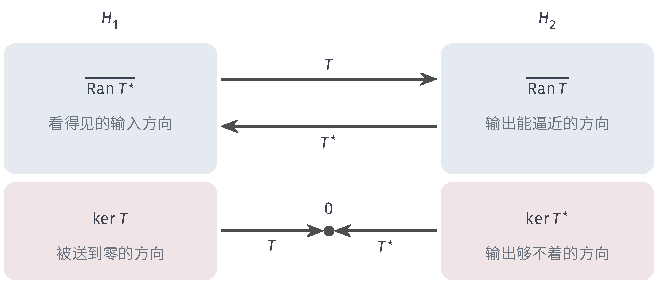
\includegraphics[width=111.404mm]{figures/04-spaces-measures-and-geometry/03-function-spaces/tikz/lop-four-subspaces/figure.pdf}
  \caption{伴随与像、零空间的正交关系。输入空间$H_1$分解为$\overline{\operatorname{Ran}T^*}$与$\ker T$，输出空间$H_2$分解为$\overline{\operatorname{Ran}T}$与$\ker T^*$。$T$把$\ker T$送到零，其余方向的像落在$\operatorname{Ran}T$中；$T^*$把$\ker T^*$送到零。无限维中像未必闭，正交关系只确定像的闭包。}
  \label{fig:lop-four-subspaces}
\end{BookInlineFigure}

\paragraph{像稠密而不闭}
闭包在无限维中不能省去。回到$\ell^2$上的对角算子$A(x_n)=(x_n/n)$。逐项核对可知$A^*=A$，且$A$是单射，所以$\ker A^*=\{0\}$，由式~\eqref{eq:lop-range-kernel}，$\operatorname{Ran}A$在$\ell^2$中稠密。

考察$y=(1/n)$，它满足$\sum_n1/n^2<\infty$，属于$\ell^2$。若$Ax=y$，逐个坐标比较得$x_n=1$，这个唯一的候选不是平方可和的，所以$y\notin\operatorname{Ran}A$。

截断候选可以看清发生了什么。令$x^{(N)}$为前$N$个坐标为$1$、其余为$0$的序列，则
\[
 \lVert Ax^{(N)}-y\rVert^2=\sum_{n>N}\frac{1}{n^2}\to0,\qquad\lVert x^{(N)}\rVert=\sqrt N\to\infty .
\]
残差趋于零，说明$y$在像的闭包中；为了取得这些越来越好的近似，输入的范数却无限增大。$y$是“只能逼近”的输出，而不是“真正属于像”的输出。

累积积分$V$给出同样的现象。若$V^*g=0$，则$\int_t^1g=0$对一切$t$成立，于是$g$在每个区间上积分为零，即$g$与一切区间示性函数正交。区间示性函数的线性组合在$L^2(0,1)$中稠密（第~\ref{chap:wavelet-transform}章用二分阶梯函数证明了这一点），所以$g=0$几乎处处，$\ker V^*=\{0\}$，$\operatorname{Ran}V$稠密。

但$\operatorname{Ran}V$中的函数都连续，阶跃函数$\mathbf 1_{(1/2,1)}$不在其中，所以$\operatorname{Ran}V\neq L^2(0,1)$。

因此，$v\perp\ker T^*$只能保证$v$在像的闭包中，不能保证方程$Tx=v$精确可解。只有已知$\operatorname{Ran}T$闭时，才有$\operatorname{Ran}T=(\ker T^*)^\perp$，这时可解性等价于与$\ker T^*$正交。何时像闭、近似解的输入为何会爆炸，是第~\ref{chap:linear-operator-equations}章的问题。

\subsection{自伴算子}
\label{sec:lop-self-adjoint}

当输入与输出在同一个Hilbert空间$H$中时，$T$与$T^*$都属于$\mathcal B(H)$，可以直接比较。实对称矩阵与复Hermite矩阵的伴随就是它自己，下面把这一性质推广到一般Hilbert空间。

\begin{definition}[自伴算子]
\label{def:lop-self-adjoint}
设$T\in\mathcal B(H)$。若$T^*=T$，即
\begin{equation}
 \langle v,Tx\rangle=\langle Tv,x\rangle\qquad(x,v\in H),
 \label{eq:lop-self-adjoint}
\end{equation}
则称$T$为\term{自伴}（self-adjoint）算子。
\end{definition}

自伴算子的二次型$\langle x,Tx\rangle$总是实数，因为
\[
 \langle x,Tx\rangle=\langle Tx,x\rangle=\overline{\langle x,Tx\rangle}.
\]
累积积分$V$不自伴，因为$V^*$从$t$累积到$1$而$V$从$0$累积到$t$；右移$S$也不自伴。

\paragraph{正交投影}
设$M$是闭子空间，$P=P_M$。对任意$x,z\in H$，$z-Pz\perp M$而$Px\in M$，所以
\[
 \langle z,Px\rangle=\langle Pz,Px\rangle+\langle z-Pz,Px\rangle=\langle Pz,Px\rangle.
\]
同理$\langle Pz,x\rangle=\langle Pz,Px\rangle$。两式相比得$\langle z,Px\rangle=\langle Pz,x\rangle$，即$P^*=P$。正交投影是自伴的；只满足$P^2=P$而像与零空间不正交的斜投影则不是。

\paragraph{积分算子的伴随核}
矩阵的共轭转置，是把元素$K_{ij}$放到$(j,i)$位置并取共轭。积分算子的伴随也是这样，核由交换变量并取共轭得到。设$(X,\mu)$、$(Y,\nu)$是$\sigma$有限测度空间，$k\in L^2(X\times Y,\mu\otimes\nu)$，$T:L^2(Y,\nu)\to L^2(X,\mu)$由式~\eqref{eq:lop-integral-operator}给出。

\begin{theorem}[伴随核]
\label{thm:lop-adjoint-kernel}
在上述条件下，$T^*:L^2(X,\mu)\to L^2(Y,\nu)$是以$k^*(y,x)=\overline{k(x,y)}$为核的积分算子，即
\begin{equation}
 (T^*g)(y)=\int_X\overline{k(x,y)}g(x)\,\mathrm d\mu(x).
 \label{eq:lop-adjoint-kernel}
\end{equation}
\end{theorem}

\begin{proof}
任取$f\in L^2(\nu)$、$g\in L^2(\mu)$。函数$(x,y)\mapsto\lvert g(x)\rvert\,\lvert k(x,y)\rvert\,\lvert f(y)\rvert$在乘积空间上可积：由乘积空间中的Cauchy--Schwarz不等式，它的积分不超过$\lVert k\rVert_{L^2}$乘以$(x,y)\mapsto\lvert g(x)f(y)\rvert$的$L^2$范数，后者由Tonelli定理等于$\lVert g\rVert\,\lVert f\rVert$。

于是可以用Fubini定理交换积分次序：
\[
 \begin{aligned}
 \langle g,Tf\rangle&=\int_X\overline{g(x)}\int_Yk(x,y)f(y)\,\mathrm d\nu(y)\,\mathrm d\mu(x)\\
 &=\int_Y\overline{\Bigl(\int_X\overline{k(x,y)}g(x)\,\mathrm d\mu(x)\Bigr)}f(y)\,\mathrm d\nu(y).
 \end{aligned}
\]
$k^*$在$Y\times X$上平方可积，由定理~\ref{thm:lop-hs-bounded}，括号中的函数属于$L^2(\nu)$。上式说明它满足伴随的定义式，由唯一性，它就是$T^*g$。
\end{proof}

当$X=Y$且$\mu=\nu$时，若$k(x,y)=\overline{k(y,x)}$对$\mu\otimes\mu$几乎处处的$(x,y)$成立，则$k^*=k$几乎处处，由定理得$T^*=T$，积分算子自伴。实值核的这一条件就是对称性$k(x,y)=k(y,x)$，相当于矩阵的对称。条件只需几乎处处成立：在零测集上改动核不改变积分算子。

贯穿例子的$1+xz$是实对称核，所以式~\eqref{eq:lop-running-kernel}给出自伴算子。累积积分的核$\mathbf 1_{\{t<s\}}$关于对角线不对称，伴随核是它的镜像，图~\ref{fig:lop-kernel-adjoint}用方格画出了这个下三角矩阵及其转置。

\begin{BookInlineFigure}
  \centering
  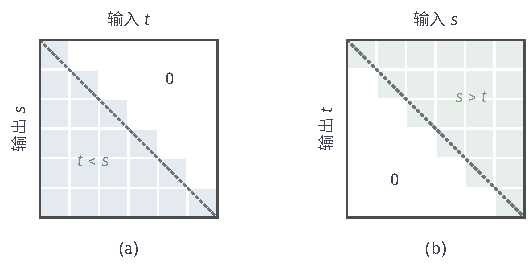
\includegraphics[width=89.623mm]{figures/04-spaces-measures-and-geometry/03-function-spaces/tikz/lop-kernel-adjoint/figure.pdf}
  \caption{积分核与伴随核关于对角线互为镜像，方格表示把区间六等分后的矩阵，虚线是连续极限下的边界，列从左到右、行从上到下对应变量增大。(a)$V$的核$\mathbf 1_{\{t<s\}}$，填色处取值$1$，是下三角矩阵。(b)伴随$V^*$的核$\mathbf 1_{\{s>t\}}$，是上三角矩阵。两核不相等，所以$V$不自伴。}
  \label{fig:lop-kernel-adjoint}
\end{BookInlineFigure}

\subsection{正算子}
\label{sec:lop-positive}

自伴保证二次型$\langle x,Tx\rangle$是实数，但这个实数可正可负。很多场合需要它非负：例如$\langle x,T^*Tx\rangle=\lVert Tx\rVert^2$度量输出的能量。这相当于矩阵的半正定，给出比自伴更强的条件。

\begin{definition}[正算子]
\label{def:lop-positive-operator}
设$T\in\mathcal B(H)$自伴。若
\begin{equation}
 \langle x,Tx\rangle\geq0\qquad(x\in H),
 \label{eq:lop-positive}
\end{equation}
则称$T$为\term{正算子}（positive operator），记作$T\geq0$。
\end{definition}

两个基本例子是正交投影与$T^*T$。对正交投影，
\[
 \langle x,Px\rangle=\langle Px,Px\rangle=\lVert Px\rVert^2\geq0.
\]
对任意$T\in\mathcal B(H_1,H_2)$，$T^*T\in\mathcal B(H_1)$自伴，因为$(T^*T)^*=T^*T^{**}=T^*T$，并且
\[
 \langle x,T^*Tx\rangle=\langle Tx,Tx\rangle=\lVert Tx\rVert^2\geq0.
\]

\paragraph{自伴条件与二次型非负条件}
定义把两个条件分开写出，因为在实空间中二次型非负并不能推出自伴。平面上逆时针旋转$90^\circ$的矩阵
\[
 \bm R=\begin{bmatrix}0&-1\\1&0\end{bmatrix}
\]
满足$\bm x^{\top}\bm R\bm x=-x_1x_2+x_2x_1=0$，二次型非负，却不对称。

复Hilbert空间中情况不同：二次型对一切$x$取实值已经迫使算子自伴。记$B=T-T^*$，它的二次型为
\[
 \langle x,Bx\rangle=\langle x,Tx\rangle-\langle Tx,x\rangle=2\mathrm i\operatorname{Im}\langle x,Tx\rangle=0.
\]

把$x+v$代入$\langle x,Bx\rangle=0$并展开，得到
\[
 \langle x,Bv\rangle+\langle v,Bx\rangle=0.
\]
再把$v$换成$\mathrm iv$，由第一个变量的共轭线性，得到
\[
 \mathrm i\langle x,Bv\rangle-\mathrm i\langle v,Bx\rangle=0.
\]
两式合起来给出$\langle x,Bv\rangle=0$对一切$x,v$成立，所以$B=0$。

为了使定义在实、复两种情形下一致，我们仍把自伴列为前提。反过来，自伴也不推出二次型非负，下面的积分算子就是例子。

\paragraph{积分算子的正性}
对$L^2(\mu)$上满足$k(x,y)=\overline{k(y,x)}$的平方可积核，自伴积分算子的正性由积分二次型检验：
\begin{equation}
 \langle f,Tf\rangle=\iint\overline{f(x)}\,k(x,y)\,f(y)\,\mathrm d\mu(y)\,\mathrm d\mu(x)\geq0\qquad(f\in L^2(\mu)).
 \label{eq:lop-integral-positive}
\end{equation}
这是矩阵半正定条件$\bm f^*\bm K\bm f\geq0$的连续版本。

贯穿例子中，
\[
 \langle f,Tf\rangle=\Bigl\lvert\int f\,\mathrm d\mu\Bigr\rvert^2+\Bigl\lvert\int zf\,\mathrm d\mu\Bigr\rvert^2\geq0,
\]
所以它是正算子。把核换成$1-6xz$，算子仍自伴，但取$f=x$，由$\int z\,\mathrm d\mu=0$与$\int z^2\,\mathrm d\mu=1/3$得
\[
 Tf=-2x,\qquad\langle f,Tf\rangle=-2\int x^2\,\mathrm d\mu=-\frac23<0,
\]
它不是正算子。

\paragraph{核逐点非负不等于正算子}
矩阵元素全为正的矩阵未必半正定，核也是如此。取两点集合$\{1,2\}$配计数测度，此时$L^2$就是$\mathbb F^2$，积分就是求和。核$k(1,1)=k(2,2)=0$、$k(1,2)=k(2,1)=1$逐点非负且对称，对应的算子交换两个坐标，矩阵为$\left[\begin{smallmatrix}0&1\\1&0\end{smallmatrix}\right]$。

取$f=(1,-1)$，$Tf=(-1,1)$，于是$\langle f,Tf\rangle=-2<0$。

反方向也不成立：核$k(x,z)=xz$在$x=1,z=-1$处为负，却给出
\[
 \langle f,Tf\rangle=\Bigl\lvert\int zf\,\mathrm d\mu\Bigr\rvert^2\geq0
\]
的正算子。正性是关于所有输入的二次型的条件，不能由核在单个点上的符号判断。

\section{紧算子}
\label{sec:lop-compact}

有界算子把有界输入变成有界输出，但无限维空间中有界序列未必有收敛子列，所以有界性本身不保证输出能被有限多个代表近似。本节要求有界输入列的输出能选出范数收敛的子列，由此得到比有界性更强的紧性。我们先比较有限秩算子与无限维恒等算子，再在Hilbert空间中建立有限秩逼近，最后把结论用于平方可积核的积分算子。

\subsection{紧算子的定义}
\label{sec:lop-compact-def}

第~\ref{chap:topological-spaces}章把闭包紧的集合称为相对紧集；第~\ref{chap:metric-spaces}章说明，在度量空间中，集合相对紧当且仅当其中每个序列都有在全空间中收敛的子列，并且在完备度量空间中这又等价于全有界，即对每个$\varepsilon>0$都能被有限个半径$\varepsilon$的球覆盖。下面把这一性质加在算子的像上。

先看输出落在有限维空间中的情形。有界线性算子$F:X\to Y$若像$\operatorname{Ran}F$是有限维子空间，就称为\term{有限秩算子}（finite-rank operator），$\dim\operatorname{Ran}F$称为它的秩。若$\lVert x_n\rVert\leq C$，则$\lVert Fx_n\rVert\leq\lVert F\rVert C$，输出序列落在有限维空间的一个有界集合中。有限维赋范空间中所有范数等价，有界序列总有收敛子列，所以$(Fx_n)$有范数收敛的子列。

\begin{definition}[紧算子]
\label{def:lop-compact-operator}
设$X,Y$是赋范空间，$T:X\to Y$是线性算子。若$X$的闭单位球$B_X$的像$T(B_X)$在$Y$中相对紧，则称$T$为\term{紧算子}（compact operator）。等价地，对$X$中每个有界序列$(x_n)$，输出序列$(Tx_n)$都有在$Y$中按范数收敛的子列。
\end{definition}

两种说法等价，是因为有界序列经缩放后落在某个$rB_X$中，而$T(rB_X)=rT(B_X)$与$T(B_X)$同时相对紧。紧算子必然有界：若$T$无界，可取单位向量$x_n$使$\lVert Tx_n\rVert\geq n$，输出序列的任何子列都无界，不可能收敛。由上一段，每个有界有限秩算子都是紧算子。

\paragraph{无限维恒等算子不紧}
紧性不是每个有界算子都具备的。设$H$是无限维Hilbert空间，取标准正交序列$(e_n)$。对$n\neq m$，$\lVert e_n-e_m\rVert^2=\lVert e_n\rVert^2+\lVert e_m\rVert^2=2$。恒等算子$I$把这个有界序列原样输出，任意两项相距$\sqrt2$，没有柯西子列，因而没有收敛子列，$I$不是紧算子。一般的无限维赋范空间中，第~\ref{chap:functions-as-vectors}章用Riesz引理说明闭单位球不紧，所以恒等算子同样不紧。

同一个序列经过$\ell^2$上的对角算子$A(x_n)=(x_n/n)$后变成$Ae_n=e_n/n$，按范数趋于零。图~\ref{fig:lop-identity-orthonormal}比较了两种输出。$A$的单位球像满足$\lvert(Ax)_n\rvert\leq1/n$，越靠后的方向被压得越扁；下一小节将用有限秩逼近证明它是紧算子。

\begin{figure}[!htb]
  \centering
  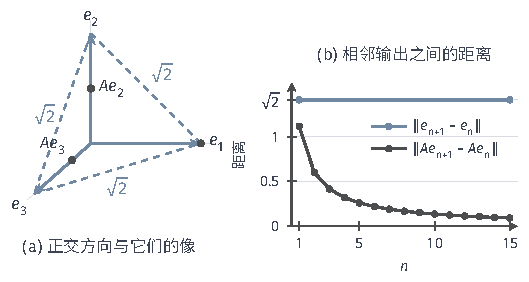
\includegraphics[width=89.6mm]{figures/02-abstract-mathematics/03-function-spaces/tikz/c3-identity-orthonormal/figure.pdf}
  \caption{同一个标准正交序列经过恒等算子与经过$A(x_n)=(x_n/n)$的对比。(a)~$e_1,e_2,e_3$两两相距$\sqrt2$（虚线），它们在$A$下的像$e_1$、$e_2/2$、$e_3/3$（黑点）向原点收拢；(b)~相邻输出的距离在恒等算子下恒为$\sqrt2$，在$A$下等于$\sqrt{1/n^2+1/(n+1)^2}$并趋于零。}
  \label{fig:lop-identity-orthonormal}
\end{figure}

这个例子说明紧性约束的对象。每个$x\in H$都能被它在前$n$个基向量上的截断任意逼近，单独看每个元素，有限截断都可行；紧性要求的却是同一个算子作用于整个有界输入族之后，输出整体可以被有限个代表覆盖。恒等算子对每个输入都能截断，对整个单位球却不能。

\paragraph{弱收敛的输入与范数收敛的输出}
第~\ref{chap:linear-functionals}章的标准正交序列满足$e_n\rightharpoonup0$而不按范数收敛。上例中$Ae_n=e_n/n$却按范数收敛到$A0=0$。这不是巧合：紧算子把弱收敛的输入变成范数收敛的输出。需要区分的是，弱收敛是输入列在全部连续线性观测下的收敛，相对紧是输出集合在范数距离下的性质，定理说明紧性在二者之间架起桥梁。

\begin{theorem}[紧算子改善收敛]
\label{thm:lop-compact-weak-strong}
设$X,Y$是赋范空间，$T:X\to Y$是紧算子。若$x_n\rightharpoonup x$，则$\lVert Tx_n-Tx\rVert\to0$。
\end{theorem}

\begin{proof}
第一步，输出弱收敛。对每个$\ell\in Y^*$，复合$\ell\circ T$是$X$上的有界线性泛函，所以$\ell(Tx_n)\to\ell(Tx)$，即$Tx_n\rightharpoonup Tx$。这一步只用到$T$有界。

第二步，反证。假设$Tx_n$不按范数收敛到$Tx$，则存在$\varepsilon>0$及子列$(x_{n_k})$，使$\lVert Tx_{n_k}-Tx\rVert\geq\varepsilon$对一切$k$成立。由第~\ref{chap:linear-functionals}章，弱收敛序列有界，所以$(x_{n_k})$有界；由紧性，可以再抽出子列，使相应的输出按范数收敛到某个$y\in Y$。

第三步，确认极限。范数收敛蕴含弱收敛，所以沿这个更细的子列，输出同时弱收敛到$y$和$Tx$。连续线性泛函能区分$Y$中不同的点（第~\ref{chap:linear-functionals}章由Hahn--Banach定理得到），弱极限唯一，故$y=Tx$。这与$\lVert Tx_{n_k}-Tx\rVert\geq\varepsilon$矛盾。
\end{proof}

对一般有界算子，第二步不成立：恒等算子把$e_n\rightharpoonup0$原样输出，输出仍只是弱收敛。

\subsection{Hilbert空间中的有限秩逼近}
\label{sec:lop-finite-rank-approx}

上面的例子提示，紧算子可以看成有限秩算子的极限。这里有两个方向：有限秩算子的算子范数极限是否紧，以及紧算子能否由有限秩算子按算子范数逼近。第一个方向在任意Banach取值空间中成立；第二个方向我们在Hilbert空间中证明。

\begin{theorem}[算子范数极限保持紧性]
\label{thm:lop-compact-limit}
设$X$是赋范空间，$Y$是Banach空间，$T_n:X\to Y$都是紧算子，$T\in\mathcal B(X,Y)$且$\lVert T_n-T\rVert\to0$。则$T$是紧算子。
\end{theorem}

\begin{proof}
$Y$完备，所以只需证明$T(B_X)$全有界：全有界集合的闭包仍全有界，又作为完备空间的闭子集完备，因而是紧集。给定$\varepsilon>0$，先取$n$使$\lVert T_n-T\rVert<\varepsilon$。$T_n(B_X)$相对紧，因而全有界，存在有限个点$y_1,\ldots,y_N\in Y$，使每个$T_nx$（$x\in B_X$）都与某个$y_i$相距小于$\varepsilon$。

对任意$x\in B_X$，选出相应的$y_i$，用三角不等式把误差拆成两段：
\[
\lVert Tx-y_i\rVert\leq\lVert(T-T_n)x\rVert+\lVert T_nx-y_i\rVert<\lVert T-T_n\rVert+\varepsilon<2\varepsilon .
\]
所以同一组$y_1,\ldots,y_N$是$T(B_X)$的有限$2\varepsilon$网。$\varepsilon$任意，$T(B_X)$全有界。
\end{proof}

关键在于误差界$\lVert T-T_n\rVert$对单位球中的全部输入同时成立，$T_n$的有限覆盖才能整体搬给$T$。若只知道$T_nx\to Tx$对每个$x$成立，就无法这样搬运：第~\ref{sec:lop-operator-convergence}节的截断投影$P_n$强算子收敛到$I$，每个$P_n$都是有限秩的，极限$I$却不紧。

\begin{example}[对角算子的有限秩逼近]
\label{ex:lop-diagonal-finite-rank}
在$\ell^2$上令$A(x_n)=(x_n/n)$，并令$A_m$只保留前$m$个坐标：$A_mx=(x_1,x_2/2,\ldots,x_m/m,0,0,\ldots)$，它的像落在前$m$个坐标张成的空间中，是有限秩算子。差$(A-A_m)x$只剩第$m+1$个坐标以后的部分，
\[
\lVert(A-A_m)x\rVert^2=\sum_{n>m}\frac{\lvert x_n\rvert^2}{n^2}\leq\frac{1}{(m+1)^2}\sum_{n>m}\lvert x_n\rvert^2\leq\frac{\lVert x\rVert^2}{(m+1)^2},
\]
取$x=e_{m+1}$时等号成立，所以$\lVert A-A_m\rVert=1/(m+1)\to0$。由定理~\ref{thm:lop-compact-limit}，$A$是紧算子。
\end{example}

图~\ref{fig:lop-finite-rank-error}把这个误差与恒等算子的截断比较。用$P_m$逼近恒等算子时，统一误差$\lVert I-P_m\rVert$恒为$1$；对固定的$x$，误差$\lVert(I-P_m)x\rVert$趋于零，但速度依赖$x$。对角算子的截断误差则按$1/(m+1)$对全部单位输入同时下降。

\begin{figure}[!htb]
  \centering
  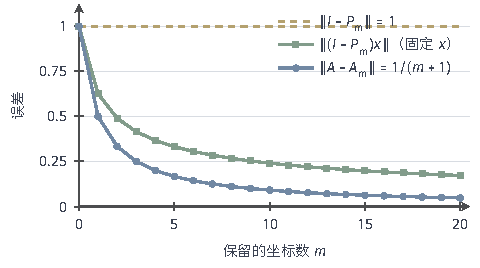
\includegraphics[width=81.2mm]{figures/02-abstract-mathematics/03-function-spaces/tikz/c3-finite-rank-error/figure.pdf}
  \caption{$\ell^2$上三种截断误差随保留坐标数$m$的变化。虚线：恒等算子的统一误差$\lVert I-P_m\rVert$恒为$1$。方点：固定单位向量$x\propto(1/n)$的误差$\lVert(I-P_m)x\rVert$趋于零，但这一速度只属于这个$x$。圆点：紧算子$A(x_n)=(x_n/n)$的统一误差$\lVert A-A_m\rVert=1/(m+1)$。}
  \label{fig:lop-finite-rank-error}
\end{figure}

\paragraph{紧算子的有限秩逼近}
现在证明反方向。思路是：紧算子的单位球像可以被有限个点以误差$\varepsilon$覆盖，这些点张成一个有限维子空间；向这个子空间作正交投影，就得到有限秩近似。正交投影的最近点性质保证投影误差不超过到覆盖点的距离。

\begin{theorem}[紧算子的有限秩逼近]
\label{thm:lop-finite-rank-approx}
设$X$是赋范空间，$H$是Hilbert空间，$T:X\to H$是紧算子。则存在有限秩算子$F_n:X\to H$，使$\lVert T-F_n\rVert\to0$。
\end{theorem}

\begin{proof}
给定$\varepsilon>0$。$T(B_X)$相对紧，因而全有界，取有限个点$y_1,\ldots,y_N$构成它的$\varepsilon$网。令$M=\operatorname{span}\{y_1,\ldots,y_N\}$，它是有限维子空间，因而闭；设$P$为到$M$的正交投影，令$F=PT$。$F$的像含于$M$，且$\lVert F\rVert\leq\lVert P\rVert\,\lVert T\rVert\leq\lVert T\rVert$，所以$F$是有界有限秩算子。

对任意$x\in B_X$，选$y_i$使$\lVert Tx-y_i\rVert<\varepsilon$。$PTx$是$M$中离$Tx$最近的点，而$y_i\in M$，所以
\[
\lVert Tx-Fx\rVert=\lVert Tx-PTx\rVert\leq\lVert Tx-y_i\rVert<\varepsilon .
\]
对$x\in B_X$取上确界得$\lVert T-F\rVert\leq\varepsilon$。令$\varepsilon=1/n$即得所需的算子列。
\end{proof}

这里控制的是整个单位球上的算子范数误差$\lVert T-F\rVert$，而不是只让$F$在有限几个输入上与$T$吻合；后者用强算子收敛就能做到，却不能保证统一误差。结合两个定理，在取值空间为Hilbert空间时，紧算子恰好是有界有限秩算子的算子范数极限。

证明真正用到的是Hilbert空间的正交投影：它把有限覆盖变成一个范数不超过$1$的线性“取最近点”操作。一般Banach空间中，有限维子空间上不一定有范数可控的投影族，紧算子能否由有限秩算子按算子范数逼近取决于空间的所谓逼近性质；确实存在不具有这一性质的Banach空间，这里不给出构造。所以本定理不能无条件推广，而定理~\ref{thm:lop-compact-limit}的方向在Banach空间中始终成立。

\subsection{积分算子的紧性}
\label{sec:lop-integral-compact}

沿用第~\ref{sec:lop-integral-bounded}小节的设定：$(X,\mu)$与$(Y,\nu)$是$\sigma$有限测度空间，$k\in L^2(X\times Y,\mu\otimes\nu)$，$T:L^2(Y,\nu)\to L^2(X,\mu)$由\eqref{eq:lop-integral-operator}给出。式\eqref{eq:lop-hs-norm}的估计对任意平方可积核成立，用于两个核之差就得到
\begin{equation}
\lVert T_k-T_{k^\prime}\rVert\leq\lVert k-k^\prime\rVert_{L^2(\mu\otimes\nu)},
\label{eq:lop-kernel-error}
\end{equation}
其中$T_k$表示以$k$为核的积分算子。所以只需用“给出有限秩算子的核”在$L^2$中逼近$k$，再用定理~\ref{thm:lop-compact-limit}。

\paragraph{分离变量的核给出有限秩算子}
若$k(x,y)=\sum_{i=1}^r\varphi_i(x)\psi_i(y)$，其中$\varphi_i\in L^2(\mu)$、$\psi_i\in L^2(\nu)$，则
\[
(Tf)(x)=\sum_{i=1}^r\Bigl(\int_Y\psi_i f\,\mathrm d\nu\Bigr)\varphi_i(x),
\]
输出落在$\operatorname{span}\{\varphi_1,\ldots,\varphi_r\}$中，$T$的秩不超过$r$。贯穿例子的核$1+xz=1\cdot1+x\cdot z$就是这样的有限和，所以\eqref{eq:lop-running-kernel}是秩为$2$的算子。最简单的分离变量核是可测矩形的示性函数$\mathbf 1_{A\times B}(x,y)=\mathbf 1_A(x)\mathbf 1_B(y)$，下面的引理说明它们的线性组合足以逼近任意可测集。

\begin{lemma}[矩形逼近]
\label{lem:lop-rectangle-approx}
设$(X,\mu)$、$(Y,\nu)$是有限测度空间，$E$属于乘积$\sigma$代数。则对每个$\varepsilon>0$，存在有限个两两不交的可测矩形，其并$R$满足$(\mu\otimes\nu)(E\,\triangle\,R)<\varepsilon$。
\end{lemma}

\begin{proof}
记$m=\mu\otimes\nu$，令$\mathcal E$为具有引理性质的可测集全体，$\mathcal R$为有限个两两不交可测矩形之并组成的族。两个矩形之交仍是矩形，矩形的补$(A\times B)^c=(A^c\times Y)\cup(A\times B^c)$是两个不交矩形之并，由此可知$\mathcal R$对有限交、补和有限并封闭。可测矩形显然属于$\mathcal E$。

若$E\in\mathcal E$，取$R\in\mathcal R$逼近它，则$R^c\in\mathcal R$且$E^c\triangle R^c=E\triangle R$，所以$\mathcal E$对补封闭。若$E_1,E_2,\ldots\in\mathcal E$，令$E=\bigcup_jE_j$。总测度有限，可取$N$使$m(E\setminus\bigcup_{j\leq N}E_j)<\varepsilon/2$；再对$j\leq N$取$R_j\in\mathcal R$使$m(E_j\triangle R_j)<\varepsilon/(2N)$。令$R=\bigcup_{j\leq N}R_j\in\mathcal R$，则
\[
m(E\triangle R)\leq m\Bigl(E\setminus\bigcup_{j\leq N}E_j\Bigr)+\sum_{j\leq N}m(E_j\triangle R_j)<\varepsilon .
\]
所以$\mathcal E$对可数并封闭。$\mathcal E$是包含全部可测矩形的$\sigma$代数，因而包含它们生成的乘积$\sigma$代数。
\end{proof}

\begin{theorem}[矩形阶梯核的稠密性]
\label{thm:lop-rectangle-dense}
形如
\begin{equation*}
\sum_{i=1}^rc_i\mathbf 1_{A_i}(x)\mathbf 1_{B_i}(y)\qquad(\mu(A_i),\nu(B_i)<\infty)
\end{equation*}
的函数在$L^2(X\times Y,\mu\otimes\nu)$中稠密。
\end{theorem}

\begin{proof}
第一步，截断到有限测度区域。由$\sigma$有限性，取递增的可测集$X_j\uparrow X$、$Y_j\uparrow Y$，且$\mu(X_j),\nu(Y_j)<\infty$。令$k_j=k\mathbf 1_{X_j\times Y_j}$，则$\lvert k-k_j\rvert^2\leq\lvert k\rvert^2$且逐点趋于零，由控制收敛定理$\lVert k-k_j\rVert_{L^2}\to0$。

第二步，用简单函数逼近。对$k_j$取简单函数$s_n\to k_j$逐点收敛且$\lvert s_n\rvert\leq\lvert k_j\rvert$（实部、虚部分别取单调逼近），则$\lvert k_j-s_n\rvert^2\leq4\lvert k_j\rvert^2$，由控制收敛定理$\lVert k_j-s_n\rVert_{L^2}\to0$。每个$s_n$是有限个$c_i\mathbf 1_{E_i}$之和，$E_i\subseteq X_j\times Y_j$可测。

第三步，用矩形代替可测集。在有限测度空间$X_j$与$Y_j$上应用引理~\ref{lem:lop-rectangle-approx}，每个$E_i$都可被有限个不交矩形之并$R_i$逼近，且$\lVert\mathbf 1_{E_i}-\mathbf 1_{R_i}\rVert_{L^2}=m(E_i\triangle R_i)^{1/2}$可任意小。三步的误差相加即得结论。
\end{proof}

\begin{theorem}[平方可积核给出紧算子]
\label{thm:lop-hs-compact}
在本小节的设定下，$T:L^2(Y,\nu)\to L^2(X,\mu)$是紧算子。
\end{theorem}

\begin{proof}
由定理~\ref{thm:lop-rectangle-dense}，对每个$\varepsilon>0$存在$k_\varepsilon(x,y)=\sum_{i=1}^rc_i\mathbf 1_{A_i}(x)\mathbf 1_{B_i}(y)$使$\lVert k-k_\varepsilon\rVert_{L^2}<\varepsilon$。$k_\varepsilon$是分离变量核，对应的积分算子把$f$送到$\sum_ic_i\bigl(\int_{B_i}f\,\mathrm d\nu\bigr)\mathbf 1_{A_i}$，是有限秩算子。由\eqref{eq:lop-kernel-error}，算子范数误差不超过$\varepsilon$。$L^2(X,\mu)$完备，由定理~\ref{thm:lop-compact-limit}，$T$是紧算子。
\end{proof}

证明中出现两种误差。$\lVert k-k_\varepsilon\rVert_{L^2(\mu\otimes\nu)}$度量的是两个核函数在乘积空间上的平方积分差，$\lVert T-T_{k_\varepsilon}\rVert$度量的是两个算子对单位输入的最坏输出差。式\eqref{eq:lop-kernel-error}只给出前者控制后者的单向关系；后者可以严格更小，正如贯穿例子中$\lVert T\rVert=1<\lVert k\rVert_{L^2}$。

图~\ref{fig:lop-rectangle-kernel}在贯穿例子上演示这一逼近。用$n\times n$网格上的格内平均作分片常数核$k_n$，它是$n^2$个矩形示性函数的线性组合，误差$\lVert k-k_n\rVert_{L^2}$大致按$1/n$下降。对这个核，分片常数逼近远不是最经济的：$k$本身的秩为$2$，两项就精确。矩形逼近的价值在于它对任意平方可积核都可行，从而在不知道核的任何具体结构时证明了紧性；按奇异值选取最经济的有限秩近似，是第~\ref{chap:operator-spectra}章的问题。

\begin{figure}[!htb]
  \centering
  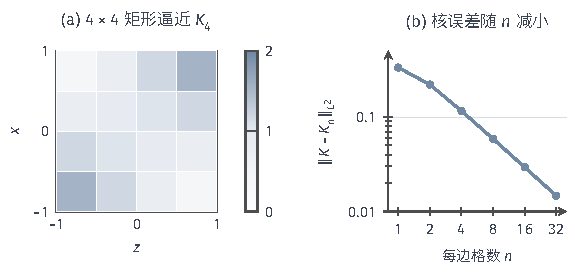
\includegraphics[width=97.4mm]{figures/02-abstract-mathematics/03-function-spaces/tikz/c3-rectangle-kernel/figure.pdf}
  \caption{用矩形示性函数的线性组合逼近核$k(x,z)=1+xz$（乘积测度由$\mathrm dz/2$给出）。(a)~$4\times4$均匀网格上取格内平均得到的分片常数核，每格对应一个可测矩形；(b)~$n\times n$网格平均的误差$\lVert k-k_n\rVert_{L^2}$，从$n=1$时的$1/3$降到$n=32$时约$0.015$，大致按$1/n$下降；它同时是相应有限秩算子的算子范数误差上界。}
  \label{fig:lop-rectangle-kernel}
\end{figure}

\section{完备空间中的基本算子定理}
\label{sec:lop-fundamental-theorems}

前面几节的估计都要求直接找到一个常数，控制单位球上的全部输入。实际问题中我们手里常常只有较弱的信息：每个固定输入上的输出有界；方程对每个右端都有唯一解；或者输入、输出同时收敛时极限相容。

对矩阵，这些信息已经足够，因为矩阵只有有限多列，每一列都有界就够了。无穷多列时，统一的常数要靠完备性来保证。三个定理都建立在第~\ref{chap:metric-spaces}章的Baire纲定理之上：完备度量空间不能写成可数个无内点闭集之并。

每个结论都要分别核对三件事：定义域是否完备，取值空间是否完备，算子是否定义在整个空间上。我们还要区分几种“好”的性质：逐输入有界与统一有界，代数上可逆（存在逆映射）与稳定可逆（逆映射有界）。

\subsection{一致有界原理}
\label{sec:lop-uniform-boundedness}

第~\ref{chap:linear-functionals}章对连续线性泛函族证明了：每个固定向量上的观测有界，整族的范数就有统一上界。这里把同样的论证用于取值于一般赋范空间的算子族，所得结论称为\term{一致有界原理}（uniform boundedness principle）。

\begin{theorem}[一致有界原理]
\label{thm:lop-uniform-boundedness}
设$X$是Banach空间，$Y$是赋范空间，$\{T_\alpha\}_{\alpha\in\Lambda}\subseteq\mathcal B(X,Y)$。若对每个$x\in X$都有$\sup_\alpha\lVert T_\alpha x\rVert<\infty$，则
\begin{equation}
 \sup_{\alpha\in\Lambda}\lVert T_\alpha\rVert<\infty.
 \label{eq:lop-uniform-boundedness}
\end{equation}
\end{theorem}

\begin{proof}
对$n\geq1$令
\[
 F_n=\{x\in X:\lVert T_\alpha x\rVert\leq n\text{ 对一切}\alpha\text{ 成立}\}.
\]
每个集合$\{x:\lVert T_\alpha x\rVert\leq n\}$是连续函数$x\mapsto\lVert T_\alpha x\rVert$的下水平集，因而闭；$F_n$是它们的交，也是闭集。由假设，每个$x$属于某个$F_n$，所以$X=\bigcup_nF_n$。

$X$完备，由Baire纲定理，某个$F_n$有内点：存在$x_0$与$r>0$使闭球$\overline B(x_0,r)\subseteq F_n$。对$\lVert z\rVert\leq r$，$x_0+z$与$x_0$都属于$F_n$，于是对一切$\alpha$，
\[
 \lVert T_\alpha z\rVert\leq\lVert T_\alpha(x_0+z)\rVert+\lVert T_\alpha x_0\rVert\leq2n .
\]
按线性缩放，$\lVert T_\alpha\rVert\leq2n/r$对一切$\alpha$成立。
\end{proof}

三个条件各司其职。算子的有界性使$F_n$闭；定义域的完备性通过Baire纲定理在某一层中找到一个球；线性把这个球平移到原点并缩放到单位球。取值空间的完备性没有用到。

定义域不完备时结论可以失败。令$X$为只有有限个非零项的序列全体，配$\ell^2$范数，它不完备。令$T_nx=nx_n$（取值于$\mathbb F$）。对每个$x\in X$，当$n$大于$x$最后一个非零项的位置时$T_nx=0$，所以$\sup_n\lvert T_nx\rvert<\infty$。

但$\lvert T_ne_n\rvert=n$，所以$\lVert T_n\rVert=n$无界。逐输入有界本身不是统一有界，二者之间的桥梁正是完备性。

\paragraph{强收敛极限的有界性}
一致有界原理回答了第~\ref{sec:lop-operator-convergence}节留下的问题。设$X$是Banach空间，$T_n\in\mathcal B(X,Y)$，且对每个$x$，$T_nx$在$Y$中收敛，记极限为$Tx$。收敛序列有界，所以$\sup_n\lVert T_nx\rVert<\infty$对每个$x$成立，由定理得
\[
 K=\sup_n\lVert T_n\rVert<\infty.
\]
于是$T$线性，并且
\[
 \lVert Tx\rVert=\lim_n\lVert T_nx\rVert\leq K\lVert x\rVert,
\]
$T$是有界算子。强算子收敛不能保证统一误差趋于零，却至少保证了统一的范数上界与极限的有界性。

\subsection{开映射定理}
\label{sec:lop-open-mapping}

由输出恢复输入，要同时满足三个要求：给定的输出有原像（存在），原像只有一个（唯一），输出上的小误差只造成输入上的小误差（稳定）。方阵可逆就同时满足这三条；无限维中它们会分离。

第~\ref{chap:topological-spaces}章把开集的像仍为开集的映射称为开映射，这与连续性要求的“开集的原像为开集”方向相反。对线性算子，开映射性质恰好给出逆向的误差估计，这就是下面的\term{开映射定理}（open mapping theorem）。

\begin{theorem}[开映射定理]
\label{thm:lop-open-mapping}
设$X,Y$是Banach空间，$T\in\mathcal B(X,Y)$是满射。则存在$\delta>0$使
\begin{equation}
 B_Y(0,\delta)\subseteq T(B_X(0,1)),
 \label{eq:lop-open-mapping}
\end{equation}
从而$T$是开映射。特别地，每个$y\in Y$都有原像$x$满足$\lVert x\rVert\leq2\delta^{-1}\lVert y\rVert$。
\end{theorem}

定理说的是：满射不仅保证每个输出都有原像，还保证能选到一个范数受控的原像。证明分两步：先用Baire纲定理得到输出球落在输入球之像的闭包中，再用逐步修正残差去掉闭包。

\begin{proof}
记$B_r=B_X(0,r)$。第一步，像的闭包含有输出球。由满射，
\[
 Y=\bigcup_kT(B_k)=\bigcup_k\overline{T(B_k)}.
\]
$Y$完备，由Baire纲定理，某个$\overline{T(B_k)}$含有开球$B_Y(y_0,\rho)$。对$\lVert y\rVert<\rho$，$y_0+y$与$y_0$都在$\overline{T(B_k)}$中，二者之差属于$\overline{T(B_k)-T(B_k)}\subseteq\overline{T(B_{2k})}$。

所以$B_Y(0,\rho)\subseteq\overline{T(B_{2k})}$。令$\eta=\rho/(2k)$，按线性缩放得
\[
 B_Y(0,\eta/2^j)\subseteq\overline{T(B_{2^{-j}})}\qquad(j\geq0).
\]

第二步，逐步修正残差。任取$\lVert y\rVert<\eta$。由第一步，存在$x_1\in B_1$使$\lVert y-Tx_1\rVert<\eta/2$。残差$y-Tx_1$落在$B_Y(0,\eta/2)$中，于是存在$x_2\in B_{1/2}$使$\lVert y-Tx_1-Tx_2\rVert<\eta/4$。如此继续，得到$x_j$满足
\[
 \lVert x_j\rVert<2^{1-j},\qquad\Bigl\lVert y-T\sum_{i\leq j}x_i\Bigr\rVert<\eta/2^j .
\]

第三步，用输入空间的完备性求和。$\sum_j\lVert x_j\rVert<2$，部分和是$X$中的柯西列；$X$完备，所以$x=\sum_jx_j$存在且$\lVert x\rVert<2$。由$T$连续，$Tx=y$。这说明$B_Y(0,\eta)\subseteq T(B_2)$，取$\delta=\eta/2$即得式~\eqref{eq:lop-open-mapping}。

第四步，验证开映射。设$U\subseteq X$开，$x\in U$，取$\varepsilon>0$使$B_X(x,\varepsilon)\subseteq U$。则
\[
 T(U)\supseteq Tx+\varepsilon T(B_1)\supseteq B_Y(Tx,\varepsilon\delta),
\]
所以$T(U)$开。

最后证明原像的估计。设$y\neq0$，$y^\prime=\delta y/(2\lVert y\rVert)$落在$B_Y(0,\delta)$中，由式~\eqref{eq:lop-open-mapping}有$x^\prime\in B_1$使$Tx^\prime=y^\prime$。令$x=2\lVert y\rVert x^\prime/\delta$，则$Tx=y$且$\lVert x\rVert\leq2\delta^{-1}\lVert y\rVert$。
\end{proof}

第一步只得到闭包：闭包中的点只能被像逼近，未必是像。第二步把“可以逼近”变成“可以达到”，代价是输入球的半径从$1$放大到$2$，并且必须用到$X$的完备性。图~\ref{fig:lop-open-mapping}用一个二维线性映射画出这个修正过程。

\begin{BookInlineFigure}
  \centering
  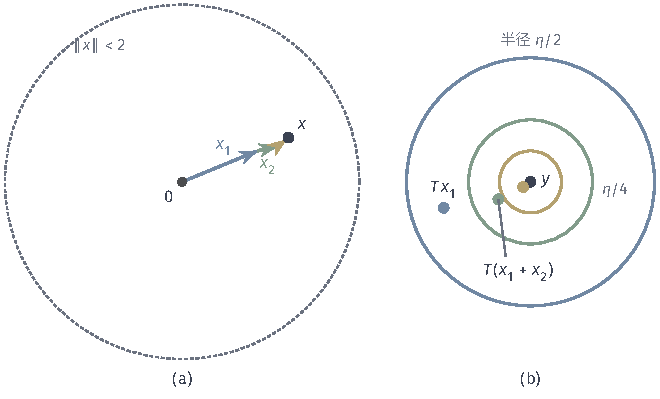
\includegraphics[width=111.725mm]{figures/04-spaces-measures-and-geometry/03-function-spaces/tikz/lop-open-mapping/figure.pdf}
  \caption{开映射定理证明中的残差修正，取$T=\operatorname{diag}(1,0.7)$，$\eta=1$作示意。(a)输入空间中修正量满足$\lVert x_j\rVert<2^{1-j}$，部分和收敛到原像$x$，$\lVert x\rVert<2$（虚线圆）。(b)输出空间中，近似$Tx_1$落在以$y$为心、半径$\eta/2$的圆内（蓝），加上修正后$T(x_1+x_2)$落入半径$\eta/4$的圆内（绿），第三次修正落入半径$\eta/8$的圆内（黄）。}
  \label{fig:lop-open-mapping}
\end{BookInlineFigure}

把开映射定理用于双射，原像的选取就是唯一的，于是逆映射自动连续。这一推论称为\term{有界逆定理}（bounded inverse theorem）。

\begin{theorem}[有界逆定理]
\label{thm:lop-bounded-inverse}
设$X,Y$是Banach空间，$T\in\mathcal B(X,Y)$是双射。则$T^{-1}\in\mathcal B(Y,X)$，并且
\begin{equation}
 \lVert T^{-1}\rVert\leq\delta^{-1},
 \label{eq:lop-bounded-inverse}
\end{equation}
其中$\delta$为开映射定理中的常数。
\end{theorem}

\begin{proof}
$T^{-1}$的线性来自$T$的线性。设$y\neq0$，$0<t<\delta$，由式~\eqref{eq:lop-open-mapping}，$ty/\lVert y\rVert$有原像落在$B_X(0,1)$中；$T$是单射，所以这个原像就是$T^{-1}(ty/\lVert y\rVert)$。于是
\[
 \lVert T^{-1}y\rVert<\frac{\lVert y\rVert}{t}.
\]
令$t\to\delta$，得$\lVert T^{-1}y\rVert\leq\delta^{-1}\lVert y\rVert$。
\end{proof}

\paragraph{代数可逆与稳定可逆}
有界逆定理说，在Banach空间之间，有界线性双射自动是稳定的：代数可逆就推出稳定可逆。条件不能省。$\ell^2$上的对角算子$A$是单射，它把$\ell^2$一一地映到像$\operatorname{Ran}A$上，在像上有逆映射$A^{-1}(y_n)=(ny_n)$。

这个逆相当于对角矩阵$\operatorname{diag}(1,2,3,\ldots)$，它无界：$\lVert A^{-1}e_n\rVert=n$，输出上$e_n/n$大小的误差会在恢复时变成长度为$1$的输入误差。原因在于$\operatorname{Ran}A$只是$\ell^2$中稠密而不闭的子空间（第~\ref{sec:lop-range-kernel}小节），按$\ell^2$范数不完备，定理的条件不成立。

开映射提供的正是局部误差估计：在原点附近半径$\delta$的输出球中，每个输出都有半径$1$以内的原像。线性把这一局部信息推广到所有尺度，就得到$\lVert T^{-1}y\rVert\leq\delta^{-1}\lVert y\rVert$。代数可逆只给出逆映射的存在；稳定可逆还要求这个统一的常数，二者在完备空间之间才自动重合。

\paragraph{两个完备范数的比较}
有界逆定理的一个直接用途是比较范数。设线性空间$X$在两个范数$\lVert\cdot\rVert_a$、$\lVert\cdot\rVert_b$下都完备，且$\lVert x\rVert_a\leq C\lVert x\rVert_b$。

恒等映射作为从$(X,\lVert\cdot\rVert_b)$到$(X,\lVert\cdot\rVert_a)$的映射是有界双射，其逆也有界，于是存在$C^\prime$使$\lVert x\rVert_b\leq C^\prime\lVert x\rVert_a$，两个范数等价。第~\ref{sec:lop-inclusions}节的$C[0,1]$上，$\lVert f\rVert_1\leq\lVert f\rVert_\infty$而两范数不等价，这与定理并不矛盾：$C[0,1]$在$\lVert\cdot\rVert_1$下不完备。

\subsection{闭图判别}
\label{sec:lop-closed-graph}

直接估计$\lVert Tx\rVert\leq C\lVert x\rVert$有时很困难。另一种思路是只检验一个较弱的条件：若输入$x_n\to x$，并且输出$Tx_n$也收敛到某个$y$，那么$y$是否必定等于$Tx$？这个条件不要求先证明输出收敛，只要求输入、输出同时收敛时极限相容。写成几何语言，就是算子的图
\begin{equation}
 \mathcal G(T)=\{(x,Tx):x\in D(T)\}\subseteq X\times Y
 \label{eq:lop-graph}
\end{equation}
在乘积范数$\lVert(x,y)\rVert=\lVert x\rVert+\lVert y\rVert$下是闭集。

$X,Y$都完备时，$X\times Y$也完备。下面的\term{闭图定理}（closed graph theorem）说明，对定义在整个完备空间上的算子，这个较弱的条件已经足够。

\begin{theorem}[闭图定理]
\label{thm:lop-closed-graph}
设$X,Y$是Banach空间，$T:X\to Y$是定义在整个$X$上的线性算子。则$T$有界当且仅当$\mathcal G(T)$在$X\times Y$中闭。
\end{theorem}

\begin{proof}
若$T$有界，$x_n\to x$推出$Tx_n\to Tx$，所以$Tx_n\to y$时$y=Tx$，图闭。

反过来，设图闭。它是Banach空间$X\times Y$的闭线性子空间，本身是Banach空间。第一坐标投影$\pi(x,Tx)=x$是从$\mathcal G(T)$到$X$的有界线性映射，因为$\lVert x\rVert\leq\lVert(x,Tx)\rVert$。它是双射，因为$T$定义在整个$X$上，每个$x$恰好对应图中一点。

由有界逆定理，$\pi^{-1}$有界：存在$C$使
\[
 \lVert x\rVert+\lVert Tx\rVert\leq C\lVert x\rVert,
\]
于是$\lVert Tx\rVert\leq C\lVert x\rVert$。
\end{proof}

图闭的条件同时考察输入与输出的极限：只知道$x_n\to x$而不知道$Tx_n$是否收敛，就无从检验；只看输出收敛而不管输入，也不能确定极限属于谁的图。定理的作用是把这个“两侧相容”的条件升级为有界性，代价是要求定义域为整个Banach空间。

\paragraph{处处有定义的对称算子有界}
设$T:H\to H$定义在整个Hilbert空间上，且$\langle v,Tx\rangle=\langle Tv,x\rangle$对一切$x,v$成立。若$x_n\to x$且$Tx_n\to w$，则对任意$v$，
\[
 \langle v,w\rangle=\lim_n\langle v,Tx_n\rangle=\lim_n\langle Tv,x_n\rangle=\langle Tv,x\rangle=\langle v,Tx\rangle ,
\]
所以$w=Tx$，图闭，$T$有界。这里没有估计任何范数，只用了对称性和内积的连续性。反过来说，无界的对称算子，例如适当定义域上的微分算子，不可能定义在整个Hilbert空间上。

\paragraph{定义域只是子空间时}
若$T$只定义在子空间$D(T)\subseteq X$上，图闭不再推出有界。回到求导$D:C^1[0,1]\subseteq C[0,1]\to C[0,1]$，两侧都用一致范数。它的图是闭的：若$f_n\to f$且$f_n^\prime\to g$都按一致范数，则在
\[
 f_n(x)=f_n(0)+\int_0^xf_n^\prime(t)\,\mathrm dt
\]
两边取极限，一致收敛允许在积分号下取极限，得到
\[
 f(x)=f(0)+\int_0^xg(t)\,\mathrm dt.
\]
所以$f\in C^1[0,1]$且$f^\prime=g$。

可是第~\ref{sec:lop-derivative-boundedness}小节已经用$\sin(2\pi nx)$说明$D$在一致范数下无界。两者不矛盾：$D(D)=C^1[0,1]$在一致范数下不完备，闭图定理的条件不满足。图闭的算子称为\term{闭算子}（closed operator）。

\paragraph{图范数}
对闭算子$T$，在定义域上换用\term{图范数}（graph norm）
\begin{equation}
 \lVert x\rVert_T=\lVert x\rVert_X+\lVert Tx\rVert_Y.
 \label{eq:lop-graph-norm}
\end{equation}
映射$x\mapsto(x,Tx)$把$(D(T),\lVert\cdot\rVert_T)$等距地映到图$\mathcal G(T)$上。当$X,Y$完备时，图作为闭子空间完备，所以$(D(T),\lVert\cdot\rVert_T)$是Banach空间，而$\lVert Tx\rVert_Y\leq\lVert x\rVert_T$说明$T$在新范数下有界。

对求导，图范数正是$\lVert f\rVert_{C^1}$。这就兑现了第~\ref{sec:lop-derivative-boundedness}小节的说法：配上$C^1$范数后定义域完备，同一个作用规则成为Banach空间之间的有界算子。

因此，把基本定理用于定义在真子空间上的算子之前，必须先确认所用的范数使定义域完备。第~\ref{chap:sobolev-spaces}章的Sobolev范数沿用同样的思想，用积分范数同时控制函数和它的弱导数。

\section{本章小结}
\label{sec:lop-summary}

本章把函数到函数的变换写成线性算子，并始终把定义域、取值空间和两侧的范数当作算子的一部分。恒等、投影与乘以有界函数自然定义在整个空间上；积分公式要由核、测度与输入空间共同保证有意义；求导只能定义在可导函数组成的真子空间上。说一个算子“有界”，就是说存在统一常数$C$使$\lVert Tx\rVert\leq C\lVert x\rVert$；对线性算子，这等价于连续与Lipschitz连续，最小的这种常数就是算子范数，它统一控制输入差造成的输出差。

同一个公式在不同范数下可以有完全不同的行为。求导在一致范数下无界，在$C^1$范数下有界；平方可积核给出有界积分算子，且$\lVert T\rVert\leq\lVert k\rVert_{L^2}$。包含映射把“同一个函数在不同空间中的大小”变成算子的有界性：有限测度上$L^q$连续嵌入$L^p$（$p\leq q$），计数测度上方向相反；改变测度时先由绝对连续性保证等价类的对应，再由密度的上下界决定有界性与范数等价。算子列的范数收敛给出统一误差，强算子收敛只给出逐输入误差，截断投影说明两者确实不同。

Hilbert空间中，伴随把输出方向拉回输入空间，给出$(\operatorname{Ran}T)^\perp=\ker T^*$与$\overline{\operatorname{Ran}T}=(\ker T^*)^\perp$；像未必闭，与$\ker T^*$正交的输出只能被逼近，未必真正可达。自伴是同一空间上$T=T^*$的附加结构，正性还要求二次型非负，二者都不能由核在个别点上的符号判断。紧算子把有界输入列变成有收敛子列的输出列，把弱收敛改善为范数收敛；在Hilbert空间中它们恰好是有限秩算子的算子范数极限，平方可积核的积分算子都是紧算子，核的$L^2$误差控制算子范数误差。

完备性把较弱的信息升级为统一控制：一致有界原理由逐输入有界得到统一的范数上界，开映射定理与有界逆定理由满射与双射得到稳定的逆，闭图定理由图的闭性得到有界性。这些结论都需要定义域与取值空间完备，定义在真子空间上的算子须先换用使定义域完备的图范数。第~\ref{chap:operator-spectra}章在这些基础上研究$T-\lambda I$何时可逆，并为紧自伴算子与一般紧算子建立特征展开和奇异分解；给定输出求解算子方程的可解性与稳定性，留到第~\ref{chap:linear-operator-equations}章。


\chapter{算子谱}
\label{chap:operator-spectra}
\label{chap:operator-spectra-equations}

第~\ref{chap:functions-as-vectors}章把函数看成下标连成一片的无限维向量，$f$在$x$处的取值就是下标$x$上的分量。沿着这个类比，第~\ref{chap:linear-operators}章的线性算子就是无限维的矩阵：积分算子的核$k(x,y)$像矩阵元$a_{jk}$，积分$\int k(x,y)f(y)\,\mathrm dy$像求和$\sum_k a_{jk}x_k$。本章继续问矩阵论最核心的问题：一个算子能否沿某些方向简单地伸缩？

对矩阵，这个问题由特征值和奇异值回答。对称矩阵在一组标准正交基下成为对角矩阵，一般矩阵用输入、输出两组标准正交方向写成伸缩的叠加。表~\ref{tab:ospec-dictionary}列出本章要沿用的对应关系。

\begin{table}[!htb]
  \centering
  \caption{矩阵与算子的对应。左列是有限维中的已知对象，右列是函数空间中的对应物。}
  \label{tab:ospec-dictionary}
  \begin{tabular}{@{}ll@{}}
    \toprule
    矩阵 & 算子\\
    \midrule
    向量$\bm x$，分量$x_k$ & 函数$f$，分量$f(x)$\\
    矩阵$\bm A$，元素$a_{jk}$ & 积分算子，核$k(x,y)$\\
    对角矩阵$\operatorname{diag}(a_k)$ & 乘法算子$(Mf)(x)=a(x)f(x)$\\
    特征值 & 谱\\
    对称矩阵的正交对角化 & 紧自伴算子的谱分解\\
    奇异值分解 & 紧算子的奇异分解\\
    Frobenius范数 & 核的$L^2$范数\\
    \bottomrule
  \end{tabular}
\end{table}

类比有一处要特别当心。矩阵$\bm A-\lambda\bm I$不可逆时一定存在特征向量，无限维中却不然：乘以$x$的算子是一个“连续的对角矩阵”，对角元铺满整个区间，却没有一个特征函数。谱里多出来的这些点，是矩阵论中没有的现象，称为连续谱和剩余谱，第~\ref{sec:ospec-spectrum}节专门分析它们。

本章从方程$(T-\lambda I)u=g$能否对一切右端稳定求解出发，逐步加条件。第~\ref{sec:ospec-spectrum}节对一般有界算子定义谱。第~\ref{sec:ospec-compact-spectrum}节加入紧性，非零谱重新变成离散的特征值。第~\ref{sec:ospec-compact-self-adjoint}节再加入自伴性，得到正交的特征方向和展开式。

自伴性要求输入与输出在同一个空间，并排除了很多重要算子。第~\ref{sec:ospec-singular}节对两个Hilbert空间之间的一般紧算子建立奇异分解。第~\ref{sec:ospec-integral-expansion}节回到平方可积核，把这些展开写成核函数的展开，并比较核的$L^2$误差与算子范数误差。

有界性、伴随、紧性、有限秩逼近和有界逆定理都来自第~\ref{chap:linear-operators}章。谱回答的是“算子沿哪些方向怎样作用”，由输出恢复输入是否稳定，要到第~\ref{chap:linear-operator-equations}章讨论两类算子方程时才系统处理。

\section{谱}
\label{sec:ospec-spectrum}

在$n$维复空间中，$\bm A-\lambda\bm I$不可逆当且仅当它不是单射，即存在非零向量$\bm v$使$\bm A\bm v=\lambda\bm v$。有限维中单射、满射与可逆三者等价，所以“使$\bm A-\lambda\bm I$不可逆的$\lambda$”恰好就是特征值；特征值与对称矩阵的正交对角化可参考\BookChapterRef{chap:eigen-spectral-decomposition}{卷二第4章“特征值与谱分解”}。无限维中三者不再等价，算子可以是单射而不满射，因此必须直接从可逆性出发。

本节设$X\neq\{0\}$是复Banach空间，$T\in\mathcal B(X)$。要求$T$回到同一个空间，是因为$T-\lambda I$只对这样的算子有意义。实空间上的算子可以先复化：令$X_{\mathbb C}=\{x+\mathrm iy:x,y\in X\}$，按复数规则定义数乘，令$T_{\mathbb C}(x+\mathrm iy)=Tx+\mathrm iTy$；Hilbert空间中取$\lVert x+\mathrm iy\rVert^2=\lVert x\rVert^2+\lVert y\rVert^2$，它来自内积$\langle x+\mathrm iy,u+\mathrm iv\rangle=\langle x,u\rangle+\langle y,v\rangle+\mathrm i(\langle x,v\rangle-\langle y,u\rangle)$。实空间算子的谱就指$T_{\mathbb C}$的谱。

复数域是必要的。平面上旋转$90^\circ$的实矩阵$\left[\begin{smallmatrix}0&-1\\1&0\end{smallmatrix}\right]$没有实特征值，复化后才有特征值$\pm\mathrm i$。紧算子的特殊性质留到下一节，本节只讨论一般有界算子。

\subsection{谱与预解集}
\label{sec:ospec-resolvent}

参数$\lambda$“好”的含义是：对每个右端$g\in X$，方程$(T-\lambda I)u=g$都有解（存在），解只有一个（唯一），并且$g$的小误差只引起$u$的小误差（稳定）。三条合起来，就是$T-\lambda I$有定义在整个$X$上的有界逆。

\begin{definition}[谱与预解集]
\label{def:ospec-spectrum}
若$T-\lambda I$是$X$到$X$的双射，且逆映射$(T-\lambda I)^{-1}$有界，则称$\lambda\in\mathbb C$属于$T$的\term{预解集}（resolvent set），记为$\rho(T)$，并称$R_\lambda=(T-\lambda I)^{-1}$为\term{预解算子}（resolvent operator）。预解集的补集$\sigma(T)=\mathbb C\setminus\rho(T)$称为$T$的\term{谱}（spectrum）。若存在非零$u\in X$使$Tu=\lambda u$，则称$\lambda$为$T$的\term{特征值}（eigenvalue），$u$为相应的\term{特征向量}（eigenvector），函数空间中也称特征函数。
\end{definition}

由第~\ref{chap:linear-operators}章的有界逆定理，Banach空间之间的有界线性双射自动有有界逆，所以定义中“逆有界”一项不额外增加限制；写出它，是为了强调预解参数要求在整个$X$上稳定地反解。定义也没有要求事先找到特征向量：$\lambda$进入谱，可以因为$T-\lambda I$有非零零空间（$\lambda$是特征值），也可以因为它是单射却不满射，此时方程对某些右端无解。

\paragraph{谱的有界性与闭性}
证明需要一个反解工具：若$\lVert A\rVert<1$，则$I-A$可逆。直观上，$(I-A)^{-1}$应当是几何级数$I+A+A^2+\cdots$；算子空间完备，这个级数确实收敛。

\begin{lemma}[小扰动的可逆性]
\label{lem:ospec-neumann}
设$A\in\mathcal B(X)$且$\lVert A\rVert<1$。则$I-A$有有界逆，$(I-A)^{-1}=\sum_{j\geq0}A^j$按算子范数收敛，且$\lVert(I-A)^{-1}\rVert\leq1/(1-\lVert A\rVert)$。
\end{lemma}

\begin{proof}
由复合的范数估计，$\lVert A^j\rVert\leq\lVert A\rVert^j$，所以$\sum_j\lVert A^j\rVert$是收敛的几何级数。$\mathcal B(X)$完备（第~\ref{chap:linear-operators}章），部分和$S_n=\sum_{j\leq n}A^j$按算子范数收敛到某个$S$，且$\lVert S\rVert\leq1/(1-\lVert A\rVert)$。直接相乘得$(I-A)S_n=S_n(I-A)=I-A^{n+1}$，令$n\to\infty$，由$\lVert A^{n+1}\rVert\to0$得$(I-A)S=S(I-A)=I$。
\end{proof}

这个级数及其截断误差在第~\ref{chap:linear-operator-equations}章作为求解第二类方程的方法系统讨论，这里只用它来确定谱的位置。

\begin{theorem}[谱是有界闭集]
\label{thm:ospec-spectrum-compact}
$\sigma(T)$是$\mathbb C$中的有界闭集，且$\sigma(T)\subseteq\{\lambda:\lvert\lambda\rvert\leq\lVert T\rVert\}$。对$\lambda\in\rho(T)$，有$\operatorname{dist}(\lambda,\sigma(T))\geq1/\lVert R_\lambda\rVert$。
\end{theorem}

\begin{proof}
有界性：若$\lvert\lambda\rvert>\lVert T\rVert$，写$T-\lambda I=-\lambda(I-T/\lambda)$，其中$\lVert T/\lambda\rVert<1$，由引理~\ref{lem:ospec-neumann}可逆，故$\lambda\in\rho(T)$。

闭性：设$\lambda_0\in\rho(T)$。对任意$\lambda$，
\[
T-\lambda I=(T-\lambda_0I)-(\lambda-\lambda_0)I=(T-\lambda_0I)\bigl(I-(\lambda-\lambda_0)R_{\lambda_0}\bigr).
\]
若$\lvert\lambda-\lambda_0\rvert<1/\lVert R_{\lambda_0}\rVert$，右端第二个因子由引理可逆，两个可逆有界算子的复合仍可逆，所以$\lambda\in\rho(T)$。这说明$\rho(T)$开，$\sigma(T)$闭，并且以$\lambda_0$为心、半径$1/\lVert R_{\lambda_0}\rVert$的开圆盘不含谱点。
\end{proof}

定理最后一式说明，参数越靠近谱，预解算子的范数至少要越大：反解$(T-\lambda I)u=g$的误差放大倍数在谱点附近没有上界。复Banach空间上有界算子的谱总是非空的，证明要用复变函数的Liouville定理考察预解算子关于$\lambda$的解析性，这里不给出证明；实空间不复化时，这一结论可以失败，旋转矩阵就是例子。

\subsection{谱点与特征值}
\label{sec:ospec-eigenvalues}

有限维中谱就是特征值的集合。下面的例子说明，无限维中谱可以完全不含特征值。

\paragraph{右移算子}
在$\ell^2$上令右移$S(x_1,x_2,\ldots)=(0,x_1,x_2,\ldots)$。它保持长度，$\lVert Sx\rVert=\lVert x\rVert$，所以$\lVert S\rVert=1$，并且$S$是单射。像中的序列首项必须为零，$e_1=(1,0,0,\ldots)$不在$\operatorname{Ran}S$中，所以$S$不满射，$S-0\cdot I$不可逆：$0\in\sigma(S)$。但$0$不是特征值，因为$Sx=0$只有零解。

$S$根本没有特征值。设$Sx=\lambda x$，逐坐标比较得$0=\lambda x_1$与$x_k=\lambda x_{k+1}$（$k\geq1$）。若$\lambda=0$，则$x_k=0$对一切$k$成立；若$\lambda\neq0$，由第一式$x_1=0$，再由第二式依次得$x_2=x_3=\cdots=0$。两种情形都只有零解。

谱却不小。由定理~\ref{thm:ospec-spectrum-compact}，$\sigma(S)$含于闭单位圆盘。对$\lvert\lambda\rvert<1$，第~\ref{chap:linear-operators}章给出$S^*$是左移，$(S-\lambda I)^*=S^*-\bar\lambda I$。序列$y=(1,\bar\lambda,\bar\lambda^2,\ldots)$平方可和，并满足$S^*y=(\bar\lambda,\bar\lambda^2,\ldots)=\bar\lambda y$，所以$\ker(S-\lambda I)^*\neq\{0\}$。由像与零空间的正交关系，$\operatorname{Ran}(S-\lambda I)$的闭包是$\ker(S-\lambda I)^*$的正交补，不是全空间，于是$S-\lambda I$不满射，$\lambda\in\sigma(S)$。谱是闭集，因而$\sigma(S)$是整个闭单位圆盘。

右移的谱充满一个圆盘，却没有一个特征向量。所以一般有界算子的谱不能理解为“特征值的集合”，后面基于特征向量的展开也不是所有有界算子都具备的表示。要得到特征展开，必须对算子再加条件，下一节的紧性是第一步。

\section{紧算子的非零谱}
\label{sec:ospec-compact-spectrum}

乘法算子和右移算子的谱里都有大块的区域，因为它们在无穷多个方向上都保持可观的大小：乘法算子的对角元$x$不趋于零，右移保持长度。紧算子则相反，它把有界集压成几乎有限的集合，越来越多的方向被压得越来越小。对角情形最清楚：$a_n\to0$时，$\operatorname{diag}(a_n)$可以被有限截断按算子范数逼近，所以是紧算子；$a_n$不趋于零时，有一列下标使$\lvert a_{n_k}\rvert\geq\delta>0$，单位向量$e_{n_k}$的像彼此至少相距$\sqrt2\,\delta$，算子不紧。

本节证明，这种压缩使非零谱点回到矩阵的情形：它们都是特征值，特征空间有限维，并且特征值只能向零聚集。连续谱被赶到了$0$这一个点上。

本节设$X$是复Banach空间，$T\in\mathcal B(X)$是紧算子。证明反复用到两个事实。第一，紧算子与有界算子的复合仍紧：若$K$紧、$A$有界，有界输入列经$K$后有收敛子列，再经连续的$A$仍收敛，所以$AK$紧；$KA$把有界列先变成有界列，再由$K$抽出收敛子列，所以$KA$也紧。

第二是第~\ref{chap:functions-as-vectors}章用来证明无限维闭球不紧的Riesz引理。在Hilbert空间中，单位向量可以取在子空间的正交补里，与子空间距离恰为$1$；Banach空间没有正交性，Riesz引理提供一个距离至少为$\theta$的替代品。

\begin{lemma}[Riesz引理]
\label{lem:ospec-riesz}
设$X$是赋范空间，$M\subsetneq X$是闭子空间，$0<\theta<1$。则存在单位向量$x\in X$，使$\lVert x-m\rVert\geq\theta$对一切$m\in M$成立。
\end{lemma}

\begin{proof}
取$x_0\notin M$。$M$闭，所以$d=\operatorname{dist}(x_0,M)>0$。由下确界的定义，存在$m_0\in M$使$\lVert x_0-m_0\rVert\leq d/\theta$。令$r=\lVert x_0-m_0\rVert$，$x=(x_0-m_0)/r$。对任意$m\in M$，点$m_0+rm$仍属于$M$，所以
\[
\lVert x-m\rVert=\frac{\lVert x_0-(m_0+rm)\rVert}{r}\geq\frac{d}{d/\theta}=\theta .
\]
\end{proof}

\paragraph{紧算子减去非零数乘}
矩阵中“单射推出可逆”的一个关键部分，是单射时存在正的放大下界。下面的引理说明，紧算子减去非零数乘时这一点仍然成立。

\begin{lemma}[单射推出下有界]
\label{lem:ospec-bounded-below}
设$K\in\mathcal B(X)$紧，$\mu\neq0$，且$K-\mu I$是单射。则存在$c>0$使
\begin{equation}
\lVert(K-\mu I)x\rVert\geq c\lVert x\rVert\qquad(x\in X),
\label{eq:ospec-bounded-below}
\end{equation}
从而$\operatorname{Ran}(K-\mu I)$是闭子空间。
\end{lemma}

\begin{proof}
反设不存在这样的$c$，可取单位向量$x_n$使$(K-\mu I)x_n\to0$。由紧性，可抽子列使$Kx_n\to y$。于是
\[
\mu x_n=Kx_n-(K-\mu I)x_n\to y,
\]
即$x_n\to x=y/\mu$，且$\lVert x\rVert=1$。由连续性$(K-\mu I)x=0$，这与单射矛盾。像闭的论证与引理~\ref{lem:ospec-approx-eigen}相同：下界使原像列成为柯西列，由$X$的完备性取极限即可。
\end{proof}

这里$\mu\neq0$是必需的。$\mu=0$时结论不成立，例如第~\ref{chap:linear-operators}章的对角算子$A(x_n)=(x_n/n)$是单射，而$\lVert Ae_n\rVert=1/n$，没有正的下界。

\begin{theorem}[紧算子的非零谱]
\label{thm:ospec-compact-spectrum}
设$X$是复Banach空间，$T\in\mathcal B(X)$紧，$\lambda\neq0$。则：
\begin{enumerate}
\item 特征空间$\ker(T-\lambda I)$有限维；
\item 若$T-\lambda I$是单射，则它是满射，从而$\lambda\in\rho(T)$；因此每个非零谱点都是特征值；
\item 对每个$\delta>0$，满足$\lvert\lambda\rvert\geq\delta$的特征值只有有限个；因此$\sigma(T)\setminus\{0\}$至多可数，并且只能在$0$处聚集；
\item 若$X$无限维，则$0\in\sigma(T)$。
\end{enumerate}
\end{theorem}

证明的共同思路是：若某个结构无限大，就能用Riesz引理造出一列彼此远离的单位向量，它们的像仍彼此远离，这与紧性矛盾。

\begin{proof}
（1）记$N=\ker(T-\lambda I)$，它是闭子空间，$T$在$N$上等于$\lambda I$。若$N$无限维，由Riesz引理可逐个取单位向量$y_1,y_2,\ldots\in N$，使$y_n$与$\operatorname{span}\{y_1,\ldots,y_{n-1}\}$的距离至少为$\frac12$；有限维子空间是闭的，所以引理适用。于是对$n\neq m$，
\[
\lVert Ty_n-Ty_m\rVert=\lvert\lambda\rvert\,\lVert y_n-y_m\rVert\geq\frac{\lvert\lambda\rvert}{2}.
\]
有界列$(y_n)$的像没有收敛子列，与紧性矛盾。

（2）记$B=T-\lambda I$，反设它是单射而不满射。对$n\geq1$，二项式展开给出
\[
B^n=(-\lambda)^nI+TP_n(T),
\]
其中$P_n(T)$是$T$的多项式。所以$B^n=K_n-\mu_nI$，其中$K_n=TP_n(T)$紧，$\mu_n=-(-\lambda)^n\neq0$。$B^n$是单射的复合，仍是单射，由引理~\ref{lem:ospec-bounded-below}，$Y_n=\operatorname{Ran}B^n$是闭子空间，并且
\[
X=Y_0\supseteq Y_1\supseteq Y_2\supseteq\cdots.
\]

这些包含都是严格的。$Y_1\neq Y_0$是假设。若有$n\geq1$使$Y_{n+1}=Y_n$，取最小的这样的$n$，再取$z\in Y_{n-1}\setminus Y_n$。则$Bz\in Y_n=Y_{n+1}$，可写
\[
Bz=B^{n+1}w=B(B^nw).
\]
由$B$单射，$z=B^nw\in Y_n$，矛盾。

由Riesz引理，对每个$n\geq1$取单位向量$y_n\in Y_n$，使其与$Y_{n+1}$的距离至少为$\frac12$。设$n<m$，用$T=B+\lambda I$改写
\[
Ty_n-Ty_m=\lambda y_n-z,\qquad z=-By_n+By_m+\lambda y_m .
\]
其中$By_n\in Y_{n+1}$，$By_m\in Y_{m+1}\subseteq Y_{n+1}$，$y_m\in Y_m\subseteq Y_{n+1}$，所以$z\in Y_{n+1}$，从而
\[
\lVert Ty_n-Ty_m\rVert=\lvert\lambda\rvert\,\Bigl\lVert y_n-\frac{z}{\lambda}\Bigr\rVert\geq\frac{\lvert\lambda\rvert}{2}.
\]
$(Ty_n)$没有收敛子列，与紧性矛盾。所以$B$是满射；它是有界双射，由有界逆定理$\lambda\in\rho(T)$。

（3）反设有无穷多个互不相同的特征值$\lambda_1,\lambda_2,\ldots$，$\lvert\lambda_n\rvert\geq\delta$，相应特征向量为$x_n$。先证它们线性无关。若有非平凡的线性关系，取项数最少的一个$\sum_{i\leq k}a_ix_i=0$，所有$a_i\neq0$且$k\geq2$。作用$T-\lambda_kI$，得
\[
\sum_{i<k}a_i(\lambda_i-\lambda_k)x_i=0,
\]
这是项数更少的非平凡关系，矛盾。

令$M_n=\operatorname{span}\{x_1,\ldots,x_n\}$，它们严格递增且闭，并且$(T-\lambda_nI)M_n\subseteq M_{n-1}$。由Riesz引理取单位向量$y_n\in M_n$，使其与$M_{n-1}$的距离至少为$\frac12$。对$n>m$，
\[
Ty_n-Ty_m=\lambda_ny_n-\bigl((\lambda_nI-T)y_n+Ty_m\bigr),
\]
括号中两项分别属于$M_{n-1}$与$M_m\subseteq M_{n-1}$，所以
\[
\lVert Ty_n-Ty_m\rVert\geq\frac{\lvert\lambda_n\rvert}{2}\geq\frac\delta2.
\]
这与紧性矛盾。结合（2），满足$\lvert\lambda\rvert\geq\delta$的谱点只有有限个，令$\delta=1,\frac12,\frac13,\ldots$即得其余结论。

（4）若$0\in\rho(T)$，则$I=T^{-1}T$是有界算子与紧算子的复合，是紧算子；但无限维空间中恒等算子不紧（第~\ref{chap:linear-operators}章），矛盾。
\end{proof}

结论（2）保留了矩阵的“单射推出可逆”：对$\lambda\neq0$，方程$(T-\lambda I)u=g$的唯一性已经推出对一切$g$的可解性与稳定性。乘法算子的谱$[0,1]$不可数，所以$M$不是紧算子，这与对角元不趋于零相符。

结论（4）说明$0$是例外，它在无限维中总是谱点，却不一定是特征值。下面两个例子都表明这一点，也说明$0$处正是连续谱待着的地方。

\paragraph{对角算子}
在$\ell^2$上令$A(x_n)=(x_n/n)$，第~\ref{chap:linear-operators}章已证明它紧。由$Ae_k=e_k/k$，每个$1/k$都是特征值，特征空间由$e_k$张成，是一维的。

$A$是单射，$0$不是特征值。像包含一切有限支撑序列，所以稠密；由定理的结论（4），$0\in\sigma(A)$，因此$0\in\sigma_{\mathrm c}(A)$。例如$y=(1/n)$不在像中，因为解$x_n=ny_n=1$不平方可和。

记$S_A=\{1/n:n\geq1\}\cup\{0\}$。若$\lambda\notin S_A$，则$d=\operatorname{dist}(\lambda,S_A)>0$，方程$(A-\lambda I)x=y$逐分量解出
\[
x_n=\frac{y_n}{1/n-\lambda},\qquad\lVert x\rVert\leq\frac{\lVert y\rVert}{d}.
\]
所以$\lambda\in\rho(A)$，$\sigma(A)=S_A$。取$y=e_n$并让$1/n$逼近离$\lambda$最近的谱点，可知上面的界不能改进，于是
\begin{equation}
\lVert R_\lambda\rVert=\frac{1}{\operatorname{dist}(\lambda,\sigma(A))}\qquad(\lambda\in\rho(A)).
\label{eq:ospec-diagonal-resolvent}
\end{equation}

图~\ref{fig:ospec-spectrum-resolvent}画出了这些谱点与预解范数。每个$1/n$附近范数都趋于无穷，就像矩阵的特征值；不同的是这些尖峰无穷多，并向$0$聚集。

\begin{BookInlineFigure}
  \centering
  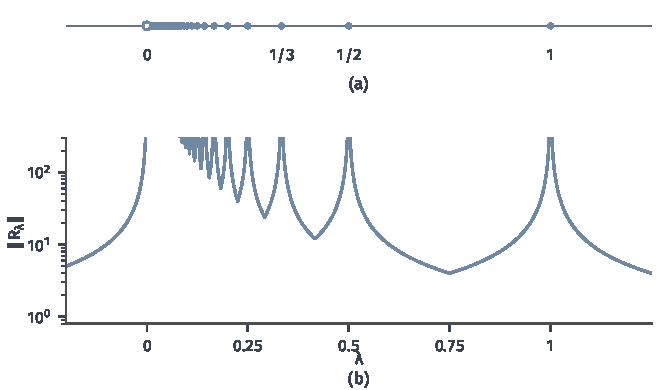
\includegraphics[width=112mm]{figures/04-spaces-measures-and-geometry/03-function-spaces/matplotlib/ospec-spectrum-resolvent/figure.pdf}
  \caption{$\ell^2$上$A(x_n)=(x_n/n)$的谱。(a)~特征值$1/n$（实心点）向$0$聚集，$0$属于谱但不是特征值（空心点）。(b)~实参数$\lambda$处预解算子的范数，纵轴取对数；各谱点处的尖峰向$0$聚集，靠近$0$时尖峰之间的低谷也越出了纵轴范围。}
  \label{fig:ospec-spectrum-resolvent}
\end{BookInlineFigure}

\paragraph{累积积分没有特征值}
紧性保证了非零谱点的有限维结构，却不保证有足够多的特征向量。在$L^2(0,1)$上令
\[
(Vf)(x)=\int_0^xf(t)\,\mathrm dt.
\]
它的核$\mathbf 1_{\{t<x\}}$平方可积，由第~\ref{chap:linear-operators}章，$V$是紧算子。

设$Vf=\lambda f$，$\lambda\neq0$。右端$Vf$连续，所以$f=\lambda^{-1}Vf$连续；于是$Vf$连续可导，$f$也连续可导。对$Vf=\lambda f$求导，并在$x=0$处取值，得到
\[
\lambda f^\prime=f,\qquad f(0)=\lambda^{-1}(Vf)(0)=0.
\]
这个初值问题的解是$f(x)=f(0)\mathrm e^{x/\lambda}=0$，所以$V$没有非零特征值。

$\lambda=0$也不是特征值。$Vf=0$说明$f$在每个区间$[0,x]$上积分为零，相减后在每个区间上积分为零。区间示性函数的线性组合在$L^2(0,1)$中稠密（第~\ref{chap:wavelet-transform}章），$f$与一个稠密集正交，只能为零。

由定理~\ref{thm:ospec-compact-spectrum}，非零谱点都是特征值，因此$\sigma(V)=\{0\}$，而$V$一个特征向量也没有。像的情况也可以判定：$V^*g(t)=\int_t^1g$，同样的论证给出$\ker V^*=\{0\}$，所以$V$的像稠密，$0$属于连续谱。

离散化可以看出这件事的矩阵对应物。把$[0,1]$分成$n$段，取$h=1/n$，累积积分变成$(\bm V_n\bm x)_i=h\sum_{j\leq i}x_j$，它是下三角矩阵，对角元全是$h$。特征值只有$h$，随$n$增大趋于$0$，与$\sigma(V)=\{0\}$相符；而$\bm V_n-h\bm I$的秩是$n-1$，整个矩阵只有一个特征方向。特征方向的严重不足，到了无限维就成了一个也没有。

\paragraph{五个例子的比较}
表~\ref{tab:ospec-gallery}汇总了本章到目前为止的算子。前三个不是紧算子，谱可以是区间或圆盘；后两个紧，谱都收缩到可数集，连续谱只剩$\{0\}$。

\begin{table}[!htb]
  \centering
  \caption{五个算子的谱。$M$是$L^2(0,1)$上乘以$x$的算子，$S$与$L$是$\ell^2$上的右移与左移，$A=\operatorname{diag}(1/n)$，$V$是累积积分；$\mathbb D$表示开单位圆盘，$\mathbb T$表示单位圆周。}
  \label{tab:ospec-gallery}
  \begin{tabular}{@{}cllll@{}}
    \toprule
    算子 & 谱 & 点谱 & 连续谱 & 剩余谱\\
    \midrule
    $M$ & $[0,1]$ & $\varnothing$ & $[0,1]$ & $\varnothing$\\
    $S$ & $\overline{\mathbb D}$ & $\varnothing$ & $\mathbb T$ & $\mathbb D$\\
    $L$ & $\overline{\mathbb D}$ & $\mathbb D$ & $\mathbb T$ & $\varnothing$\\
    $A$ & $\{1/n\}\cup\{0\}$ & $\{1/n\}$ & $\{0\}$ & $\varnothing$\\
    $V$ & $\{0\}$ & $\varnothing$ & $\{0\}$ & $\varnothing$\\
    \bottomrule
  \end{tabular}
\end{table}

表中$L$的圆周部分这样判定：$\lvert\lambda\rvert=1$时，特征方程的解$(c,c\lambda,c\lambda^2,\ldots)$不平方可和，所以$L-\lambda I$是单射；由$\ker(S-\bar\lambda I)=\{0\}$，它的像稠密；谱是闭集，圆周属于谱。

两个紧算子的对比划出了本节结论的边界。紧性把非零谱变成离散的特征值，但不保证特征向量张满空间，更不保证它们彼此正交；$V$的谱只有一个点，任何沿特征方向的展开都不存在。下一节加入自伴条件，正是为了得到正交而完备的特征方向。

\section{紧自伴算子的谱分解}
\label{sec:ospec-compact-self-adjoint}

实对称矩阵有一组由特征向量组成的标准正交基，矩阵在这组基下是实对角矩阵。上一节的累积积分说明，紧性本身不足以给出这种结构；对角算子$A(x_n)=(x_n/n)$却正好具备它：特征向量$e_n$组成标准正交基，算子就是沿每个基方向乘以一个数。二者的差别在于$A$是自伴的。本节证明，在Hilbert空间中对紧算子再加入自伴条件，就得到实特征值、正交的特征方向，以及Hilbert范数下的特征展开。

本节设$H$是实或复Hilbert空间，$T\in\mathcal B(H)$紧且自伴，即$\langle v,Tu\rangle=\langle Tv,u\rangle$对一切$u,v$成立。证明不需要复化：自伴算子的特征值将被证明是实数。

\begin{theorem}[紧自伴算子的谱分解]
\label{thm:ospec-compact-self-adjoint}
设$T$是Hilbert空间$H$上的紧自伴算子。则：
\begin{enumerate}
\item $T$的特征值都是实数，属于不同特征值的特征向量互相正交；
\item 每个非零特征值的特征空间有限维；对每个$\delta>0$，满足$\lvert\lambda\rvert\geq\delta$的特征值只有有限个；
\item 存在有限或可数的标准正交序列$(e_j)$及非零实数$\lambda_j$（按重数重复列出，$\lvert\lambda_1\rvert\geq\lvert\lambda_2\rvert\geq\cdots$，序列无限时$\lambda_j\to0$），使$Te_j=\lambda_je_j$，$(e_j)$的闭张成等于$(\ker T)^\perp$，并且对每个$u\in H$，
\begin{equation}
u=u_0+\sum_j\langle e_j,u\rangle e_j,\qquad Tu=\sum_j\lambda_j\langle e_j,u\rangle e_j,\qquad u_0\in\ker T,
\label{eq:ospec-spectral-expansion}
\end{equation}
两个级数都按$H$的范数收敛。
\end{enumerate}
\end{theorem}

证明的主线是：先说明自伴算子的范数可以由二次型$\langle u,Tu\rangle$读出，再用紧性找到使二次型绝对值最大的方向，它就是一个特征方向；然后把算子限制到这个方向的正交补上，重复同样的步骤。下面分步完成。

\paragraph{特征值与正交性}
设$Tu=\lambda u$，$u\neq0$。由内积对第一个变量共轭线性，$\langle u,Tu\rangle=\lambda\lVert u\rVert^2$，$\langle Tu,u\rangle=\bar\lambda\lVert u\rVert^2$；自伴使两者相等，所以$\lambda=\bar\lambda$是实数。再设$Tv=\mu v$，$\mu\neq\lambda$，两者都是实数，于是
\[
\lambda\langle v,u\rangle=\langle v,Tu\rangle=\langle Tv,u\rangle=\mu\langle v,u\rangle ,
\]
从而$\langle v,u\rangle=0$。这证明了结论1。

\paragraph{非零特征值的有限性}
设$(e_j)$是一列两两正交的单位特征向量，$Te_j=\lambda_je_j$且$\lvert\lambda_j\rvert\geq\delta>0$；它们可以来自同一个特征空间的标准正交组，也可以属于不同特征值（由结论1自动正交）。对$j\neq k$，
\[
\lVert Te_j-Te_k\rVert^2=\lVert\lambda_je_j-\lambda_ke_k\rVert^2=\lvert\lambda_j\rvert^2+\lvert\lambda_k\rvert^2\geq2\delta^2 ,
\]
输出列没有柯西子列，与紧性矛盾，所以这种序列只能有限长。取同一特征空间中的标准正交组，即知非零特征空间有限维；取不同特征值的特征向量，即知$\lvert\lambda\rvert\geq\delta$的特征值只有有限个。这证明了结论2，它在Hilbert空间中重现了上一节定理的相应部分，而且证明更短，因为正交性代替了Riesz引理。

\paragraph{二次型给出范数}
令$M=\sup_{\lVert u\rVert=1}\lvert\langle u,Tu\rangle\rvert$。由Cauchy--Schwarz不等式$M\leq\lVert T\rVert$。反向不等式要从二次型恢复$\lVert Tu\rVert$。自伴使$\langle u,Tv\rangle=\langle Tu,v\rangle=\overline{\langle v,Tu\rangle}$，展开可得
\[
\langle u+v,T(u+v)\rangle-\langle u-v,T(u-v)\rangle=2\langle u,Tv\rangle+2\langle v,Tu\rangle=4\operatorname{Re}\langle v,Tu\rangle .
\]
左边两项的绝对值分别不超过$M\lVert u+v\rVert^2$与$M\lVert u-v\rVert^2$，再用平行四边形恒等式$\lVert u+v\rVert^2+\lVert u-v\rVert^2=2\lVert u\rVert^2+2\lVert v\rVert^2$，得
\[
4\operatorname{Re}\langle v,Tu\rangle\leq2M\bigl(\lVert u\rVert^2+\lVert v\rVert^2\bigr).
\]
对单位向量$u$且$Tu\neq0$，取$v=Tu/\lVert Tu\rVert$，则$\operatorname{Re}\langle v,Tu\rangle=\lVert Tu\rVert$，上式化为$\lVert Tu\rVert\leq M$。因此$\lVert T\rVert=M$。

\paragraph{紧性给出极值方向}
设$T\neq0$。取单位向量$u_n$使$\lvert\langle u_n,Tu_n\rangle\rvert\to\lVert T\rVert$。这些二次型都是实数，可以抽出子列使它们的符号一致，于是$\langle u_n,Tu_n\rangle\to\lambda$，其中$\lambda=\lVert T\rVert$或$-\lVert T\rVert$。这里不能预先假定$\lambda$为正：自伴算子的二次型可以取负值，绝对值最大的特征值可能是负的。展开
\[
\lVert Tu_n-\lambda u_n\rVert^2=\lVert Tu_n\rVert^2-2\lambda\langle u_n,Tu_n\rangle+\lambda^2\leq2\lambda^2-2\lambda\langle u_n,Tu_n\rangle\to0 ,
\]
其中用到$\lVert Tu_n\rVert\leq\lVert T\rVert=\lvert\lambda\rvert$。

由紧性，可再抽子列使$Tu_n\to w$。于是$\lambda u_n=Tu_n-(Tu_n-\lambda u_n)\to w$，即$u_n\to e=w/\lambda$，$\lVert e\rVert=1$，并且$Te=\lim Tu_n=w=\lambda e$。所以$\pm\lVert T\rVert$中至少有一个是特征值，相应单位特征向量为$e$。

\paragraph{逐步分解与零空间}
记$e_1=e$，$\lambda_1=\lambda$。正交补$H_2=\{e_1\}^\perp$在$T$下不变：若$\langle e_1,v\rangle=0$，则$\langle e_1,Tv\rangle=\langle Te_1,v\rangle=\lambda_1\langle e_1,v\rangle=0$。$T$在$H_2$上的限制仍是紧自伴算子，范数不超过$\lVert T\rVert$。若这个限制为零，过程停止；否则重复上一段，得到$e_2\perp e_1$及$\lvert\lambda_2\rvert=\lVert T|_{H_2}\rVert\leq\lvert\lambda_1\rvert$。依此类推，在$H_k=\{e_1,\ldots,e_{k-1}\}^\perp$上取$e_k$。若过程不停止，由结论2，$\lambda_k\to0$。

令$M$为$(e_j)$的闭张成。$M^\perp$含于每个$H_k$，所以$T$在$M^\perp$上的限制的范数不超过每个$\lvert\lambda_k\rvert$；过程无限时它趋于零，有限时按停止条件本身为零。因此$T$在$M^\perp$上恒为零，$M^\perp\subseteq\ker T$。反过来，若$Tu=0$，则对每个$j$，
\[
\langle e_j,u\rangle=\frac{1}{\lambda_j}\langle Te_j,u\rangle=\frac{1}{\lambda_j}\langle e_j,Tu\rangle=0 ,
\]
所以$\ker T\subseteq M^\perp$。二者相等，$M=(M^\perp)^\perp=(\ker T)^\perp$。这也说明每个非零特征值都已出现在$(\lambda_j)$中：属于非零特征值$\mu$的特征向量与$\ker T$正交，因而落在$M$中；若$\mu$不等于任何$\lambda_j$，由结论1它与所有$e_j$正交，只能为零。

\paragraph{展开式}
$u$在闭子空间$M$上的正交投影为$\sum_j\langle e_j,u\rangle e_j$，级数按范数收敛（第~\ref{chap:inner-product-spaces}章）；余项$u_0=u-P_Mu$属于$M^\perp=\ker T$。把$T$作用于投影的部分和，由连续性得$Tu=\sum_j\lambda_j\langle e_j,u\rangle e_j$。这就是式\eqref{eq:ospec-spectral-expansion}，定理证毕。

\paragraph{空间的分解与有限谱截断}
定理把$H$分成两部分：$\ker T$与非零特征方向的闭张成$(\ker T)^\perp$。任意向量$u$的位置由它在$\ker T$中的分量$u_0$与各特征方向上的系数$\langle e_j,u\rangle$完全确定，$T$消去$u_0$，并把第$j$个系数乘以$\lambda_j$。由勾股定理，
\[
\lVert u\rVert^2=\lVert u_0\rVert^2+\sum_j\lvert\langle e_j,u\rangle\rvert^2,\qquad\lVert Tu\rVert^2=\sum_j\lambda_j^2\lvert\langle e_j,u\rangle\rvert^2 .
\]

只保留前$m$个特征方向，得到有限秩算子$T_mu=\sum_{j\leq m}\lambda_j\langle e_j,u\rangle e_j$。由上式，
\[
\lVert(T-T_m)u\rVert^2=\sum_{j>m}\lambda_j^2\lvert\langle e_j,u\rangle\rvert^2\leq\lambda_{m+1}^2\lVert u\rVert^2 ,
\]
取$u=e_{m+1}$时等号成立，所以$\lVert T-T_m\rVert=\lvert\lambda_{m+1}\rvert$（非零特征值用尽时约定为$0$）。特征值按绝对值递减排列，截断误差就是第一个被舍弃的特征值的绝对值；这给出第~\ref{chap:linear-operators}章有限秩逼近的一个具体而经济的选择。

\paragraph{贯穿例子}
回到$L^2([-1,1],\mu)$，$\mathrm d\mu=\mathrm dz/2$，核$1+xz$给出$(Tf)(x)=\int f\,\mathrm d\mu+x\int zf\,\mathrm d\mu$。核实对称，$T$紧自伴。由$T1=1$与$Tx=x\int z^2\,\mathrm d\mu=\tfrac13x$，单位特征向量为$e_1=1$、$e_2=\sqrt3\,x$，特征值$\lambda_1=1$、$\lambda_2=1/3$，于是
\[
Tf=\langle e_1,f\rangle e_1+\tfrac13\langle e_2,f\rangle e_2 .
\]
与$1,x$都正交的函数组成$\ker T$，例如$x^2-1/3$，这个零空间是无限维的。截断一项的误差为$\lVert T-T_1\rVert=1/3$。

把核换成$1-6xz$，常数方向不变，线性方向变为$Tx=-6x\int z^2\,\mathrm d\mu=-2x$，绝对值最大的特征值是$-2$。若只寻找正的最大特征值，就会漏掉这个主导方向，这正是证明中不预设$\lambda>0$的原因。图~\ref{fig:ospec-spectral-stretch}在两组特征方向的系数平面上画出了这两类伸缩。

\begin{figure}[!htb]
  \centering
  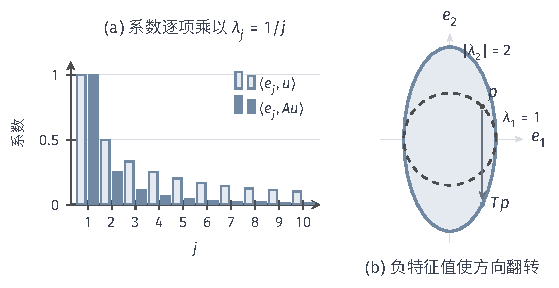
\includegraphics[width=94.6mm]{figures/02-abstract-mathematics/03-function-spaces/tikz/c3-spectral-stretch/figure.pdf}
  \caption{紧自伴算子沿特征方向逐个伸缩。(a)~$\ell^2$上$A=\operatorname{diag}(1/j)$，浅色条为$u$的系数$\langle e_j,u\rangle=1/j$，深色条为$Au$的系数$1/j^2$；(b)~$L^2([-1,1],\mathrm dz/2)$上核$1-6xz$的积分算子，在$e_1=1$、$e_2=\sqrt3x$的系数平面上把虚线单位圆映为实线椭圆：$e_1$方向乘$1$，$e_2$方向乘$-2$。与$1,x$正交的方向全部被映为零，图中未画出。}
  \label{fig:ospec-spectral-stretch}
\end{figure}

谱分解中的级数按Hilbert空间的范数收敛。对$L^2$中的函数，这意味着平方积分误差趋于零，并不意味着在每一点或一致地收敛；第~\ref{sec:ospec-integral-expansion}节在积分核上具体讨论这一区别。

\section{紧算子的奇异分解}
\label{sec:ospec-singular}

累积积分$V$没有特征向量，从$L^2(\nu)$到另一个空间$L^2(\mu)$的积分算子更谈不上$T-\lambda I$。有限维中，矩阵的奇异值分解用输入、输出各一组标准正交方向解决这个问题，可参考\BookChapterRef{chap:singular-value-decomposition}{卷二第5章“奇异值分解”}。对紧算子，同样的构造可以通过正的紧自伴算子$T^*T$完成，而不要求原算子自伴，也不要求输入与输出位于同一空间。

本节设$H_1,H_2$是Hilbert空间，$T:H_1\to H_2$是紧算子。

\paragraph{从$T^*T$构造两组方向}
$T^*T:H_1\to H_1$是紧算子，因为它是有界算子$T^*$与紧算子$T$的复合；它自伴，并且
\[
\langle x,T^*Tx\rangle=\langle Tx,Tx\rangle=\lVert Tx\rVert^2\geq0 ,
\]
所以是正算子，特征值都非负，并且$T^*Tx=0$当且仅当$Tx=0$，即$\ker(T^*T)=\ker T$。

对$T^*T$应用定理~\ref{thm:ospec-compact-self-adjoint}，得到标准正交的特征向量$v_j$与正特征值$s_j$，按递减顺序排列。令$\sigma_j=\sqrt{s_j}$，再令$u_j=Tv_j/\sigma_j$。这组输出方向也标准正交：
\[
\langle u_j,u_k\rangle=\frac{\langle Tv_j,Tv_k\rangle}{\sigma_j\sigma_k}=\frac{\langle v_j,T^*Tv_k\rangle}{\sigma_j\sigma_k}=\frac{\sigma_k^2\langle v_j,v_k\rangle}{\sigma_j\sigma_k}=\delta_{j,k} .
\]
此外$T^*u_j=T^*Tv_j/\sigma_j=\sigma_jv_j$，所以$T$把$v_j$送到$\sigma_ju_j$，$T^*$把$u_j$送回$\sigma_jv_j$。

\begin{theorem}[紧算子的奇异分解]
\label{thm:ospec-svd}
设$T:H_1\to H_2$是紧算子，$\sigma_1\geq\sigma_2\geq\cdots>0$及标准正交序列$(v_j)\subseteq H_1$、$(u_j)\subseteq H_2$如上构造。则对每个$x\in H_1$、$y\in H_2$，
\begin{equation}
Tx=\sum_j\sigma_j\langle v_j,x\rangle u_j,\qquad T^*y=\sum_j\sigma_j\langle u_j,y\rangle v_j ,
\label{eq:ospec-svd}
\end{equation}
级数按范数收敛。$(v_j)$的闭张成为$(\ker T)^\perp$，$(u_j)$的闭张成为$\overline{\operatorname{Ran}T}=(\ker T^*)^\perp$。序列无限时$\sigma_j\to0$。
\end{theorem}

\begin{proof}
由定理~\ref{thm:ospec-compact-self-adjoint}，$(v_j)$的闭张成为$(\ker T^*T)^\perp=(\ker T)^\perp$，任意$x$可写成$x=x_0+\sum_j\langle v_j,x\rangle v_j$，$x_0\in\ker T$。把$T$作用于部分和并取极限，得$Tx=\sum_j\langle v_j,x\rangle Tv_j=\sum_j\sigma_j\langle v_j,x\rangle u_j$。

由这一展开，每个$Tx$都落在$(u_j)$的闭张成中；反之每个$u_j=T(v_j/\sigma_j)$属于$\operatorname{Ran}T$。所以$(u_j)$的闭张成等于$\overline{\operatorname{Ran}T}$，再由第~\ref{chap:linear-operators}章的正交关系，它等于$(\ker T^*)^\perp$。

关于$T^*$的展开，对任意$x$有
\[
\langle x,T^*y\rangle=\langle Tx,y\rangle=\sum_j\sigma_j\overline{\langle v_j,x\rangle}\langle u_j,y\rangle=\Bigl\langle x,\sum_j\sigma_j\langle u_j,y\rangle v_j\Bigr\rangle ,
\]
右端级数因系数平方可和而收敛，两边对一切$x$相等，故展开成立。$\sigma_j\to0$来自$s_j\to0$。
\end{proof}

数$\sigma_j$称为$T$的\term{奇异值}（singular value），$v_j$与$u_j$分别称为\term{右奇异向量}（right singular vector）与\term{左奇异向量}（left singular vector），三者合称$T$的\term{奇异系统}（singular system）。函数空间中，左右奇异向量也称左右奇异函数。

展开式\eqref{eq:ospec-svd}把$T$的作用拆成三步：读出输入在$v_j$方向上的系数，乘以$\sigma_j$，再放到输出方向$u_j$上。输入空间分成$\ker T$与$\overline{\operatorname{span}}\{v_j\}$，前者的分量在输出中完全看不见；输出空间分成$\ker T^*$与$\overline{\operatorname{span}}\{u_j\}$，前者是任何输入都到达不了的方向。两组方向一般位于不同的空间；即使$H_1=H_2$，$u_j$也未必等于$v_j$。对正的紧自伴算子，两组方向可以取得相同，奇异值就是特征值；对一般自伴算子，奇异值是特征值的绝对值，负特征值的方向上$u_j=-v_j$。

\begin{example}[累积积分的奇异分解]
\label{ex:ospec-volterra-svd}
在$L^2(0,1)$上，$(Vf)(x)=\int_0^xf(t)\,\mathrm dt$是紧算子，伴随为$(V^*g)(t)=\int_t^1g(x)\,\mathrm dx$（第~\ref{chap:linear-operators}章），于是
\[
(V^*Vf)(t)=\int_t^1\Bigl(\int_0^xf(s)\,\mathrm ds\Bigr)\mathrm dx .
\]

设$V^*Vf=sf$，$s>0$。右端是连续函数，所以$f=s^{-1}V^*Vf$连续；于是$Vf$连续可导，$V^*Vf$二次连续可导，$f$也二次连续可导。对$t$求导两次得$(V^*Vf)^\prime=-Vf$、$(V^*Vf)^{\prime\prime}=-f$，因此$sf^{\prime\prime}=-f$；又由表达式直接读出$(V^*Vf)^\prime(0)=0$、$(V^*Vf)(1)=0$，故$f^\prime(0)=0$、$f(1)=0$。满足这些条件的非零解为$f(t)=c\cos(\omega t)$，其中$\omega=s^{-1/2}$且$\cos\omega=0$，即$\omega_k=(k-\tfrac12)\pi$，$k=1,2,\ldots$。

上一节已证明$V$是单射，所以$\ker V^*V=\ker V=\{0\}$，$V^*V$的特征向量张满整个$L^2(0,1)$。由此
\begin{equation*}
\begin{gathered}
\sigma_k=\frac{1}{(k-\frac12)\pi}=\frac{2}{(2k-1)\pi},\\
v_k(t)=\sqrt2\cos\bigl((k-\tfrac12)\pi t\bigr),\qquad u_k(x)=\sqrt2\sin\bigl((k-\tfrac12)\pi x\bigr),
\end{gathered}
\end{equation*}
其中$u_k=Vv_k/\sigma_k$可直接积分验证，归一化由$\int_0^12\cos^2(\omega_kt)\,\mathrm dt=1+\sin(2\omega_k)/(2\omega_k)=1$核对。前几个奇异值约为$0.637$、$0.212$、$0.127$、$0.091$，按$1/k$的速度衰减。
\end{example}

$V$没有特征向量，却有完整的奇异系统：输入方向是余弦族，输出方向是正弦族，两组方向不同。这说明奇异分解确实不依赖自伴性，它对每个紧算子都存在。

\paragraph{截断奇异分解}
只保留前$m$项，得到秩不超过$m$的算子
\[
T_mx=\sum_{j\leq m}\sigma_j\langle v_j,x\rangle u_j .
\]
下面的定理说明，截断误差恰为第一个被舍弃的奇异值，并且没有任何秩不超过$m$的算子能做得更好。正奇异值只有有限个时，约定用尽之后的$\sigma_j=0$。

\begin{theorem}[截断奇异分解的误差]
\label{thm:ospec-svd-truncation}
在定理~\ref{thm:ospec-svd}的条件下，$\lVert T-T_m\rVert=\sigma_{m+1}$；并且对每个秩不超过$m$的有界算子$F:H_1\to H_2$，都有$\lVert T-F\rVert\geq\sigma_{m+1}$。
\end{theorem}

\begin{proof}
第一步，计算截断误差。由式\eqref{eq:ospec-svd}及$(u_j)$的正交性，
\[
\lVert(T-T_m)x\rVert^2=\sum_{j>m}\sigma_j^2\lvert\langle v_j,x\rangle\rvert^2\leq\sigma_{m+1}^2\sum_{j>m}\lvert\langle v_j,x\rangle\rvert^2\leq\sigma_{m+1}^2\lVert x\rVert^2 ,
\]
最后一步是Bessel不等式。若$\sigma_{m+1}>0$，取$x=v_{m+1}$时等号成立，所以$\lVert T-T_m\rVert=\sigma_{m+1}$。

第二步，证明下界。不妨设$\sigma_{m+1}>0$。令$W=\operatorname{span}\{v_1,\ldots,v_{m+1}\}$，它是$m+1$维的。$F$把$W$映入维数不超过$m$的$\operatorname{Ran}F$，由维数公式，存在单位向量$x\in W$使$Fx=0$。写$x=\sum_{j\leq m+1}c_jv_j$，$\sum_j\lvert c_j\rvert^2=1$，则
\[
\lVert(T-F)x\rVert^2=\lVert Tx\rVert^2=\sum_{j\leq m+1}\sigma_j^2\lvert c_j\rvert^2\geq\sigma_{m+1}^2 .
\]
因此$\lVert T-F\rVert\geq\sigma_{m+1}$。
\end{proof}

图~\ref{fig:ospec-svd-decay}在累积积分上展示这一结论。保留前三项时误差为$\sigma_4\approx0.091$；奇异值衰减越快，同样秩的截断误差越小。奇异值越小的方向振荡越快：$V$是积分，它把快速振荡的输入平均掉，输出的幅度只剩$1/\omega_k$倍。对比$\ell^2$上的$A(x_n)=(x_n/n)$，它是正自伴算子，奇异值就是特征值$1/n$，左右奇异向量都是$e_n$，第~\ref{chap:linear-operators}章对它的坐标截断正是截断奇异分解。

\begin{figure}[!htb]
  \centering
  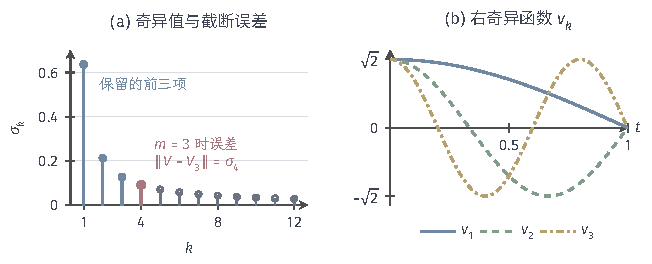
\includegraphics[width=110.3mm]{figures/02-abstract-mathematics/03-function-spaces/tikz/c3-svd-decay/figure.pdf}
  \caption{累积积分$(Vf)(x)=\int_0^xf$在$L^2(0,1)$上的奇异分解。(a)~奇异值$\sigma_k=2/((2k-1)\pi)$；保留前三项（蓝色）时，算子范数误差等于第四个奇异值$\sigma_4\approx0.091$（红色），后面的奇异值（空心）全部被舍去；(b)~前三个右奇异函数$v_k(t)=\sqrt2\cos((k-\frac12)\pi t)$，序号越大振荡越快。}
  \label{fig:ospec-svd-decay}
\end{figure}

小奇异值对正向逼近是好消息：舍去它们，误差很小。对反向求解却是坏消息：从输出恢复输入，要把这些方向上的系数除以$\sigma_j$。这一障碍是第~\ref{chap:linear-operator-equations}章讨论第一类方程时的核心问题。

\section{积分算子的谱展开}
\label{sec:ospec-integral-expansion}

第~\ref{chap:linear-operators}章证明了：$\sigma$有限测度空间上的平方可积核给出有界的紧积分算子，伴随的核是原核交换变量后取共轭，核的$L^2$误差控制算子范数误差。本节把前几节的展开落实到这些核上。算子的展开是关于输入函数$f$的级数；核是乘积空间上的一个函数，它也可以展开成乘积函数的级数。两种展开所用的收敛意义不同，这是本节要分清的主要问题。

下面设$(X,\mu)$、$(Y,\nu)$是$\sigma$有限测度空间，$k\in L^2(X\times Y,\mu\otimes\nu)$，$T:L^2(Y,\nu)\to L^2(X,\mu)$是以$k$为核的积分算子。对$a\in L^2(\mu)$、$b\in L^2(\nu)$，记$(a\otimes\bar b)(x,y)=a(x)\overline{b(y)}$。先建立两个把“核”与“算子”联系起来的工具。

\begin{lemma}[乘积函数与核系数]
\label{lem:ospec-product-coefficients}
设$(a_j)\subseteq L^2(\mu)$、$(b_l)\subseteq L^2(\nu)$都是标准正交序列。则$\{a_j\otimes\bar b_l\}$是$L^2(\mu\otimes\nu)$中的标准正交族，并且
\[
\langle a_j\otimes\bar b_l,k\rangle_{L^2(\mu\otimes\nu)}=\langle a_j,Tb_l\rangle_{L^2(\mu)} .
\]
\end{lemma}

\begin{proof}
函数$\lvert a_j(x)\rvert^2\lvert b_l(y)\rvert^2$的积分由Tonelli定理等于$\lVert a_j\rVert^2\lVert b_l\rVert^2=1$，所以$a_j\otimes\bar b_l\in L^2(\mu\otimes\nu)$。两个乘积函数之积可积（Cauchy--Schwarz），由Fubini定理分离变量，
\begin{equation*}
\begin{aligned}
\langle a_j\otimes\bar b_l,a_{j^\prime}\otimes\bar b_{l^\prime}\rangle&=\int\overline{a_j}a_{j^\prime}\,\mathrm d\mu\cdot\int b_l\overline{b_{l^\prime}}\,\mathrm d\nu\\
&=\langle a_j,a_{j^\prime}\rangle\,\langle b_{l^\prime},b_l\rangle=\delta_{j,j^\prime}\delta_{l,l^\prime}.
\end{aligned}
\end{equation*}
同样，$\overline{a_j(x)}b_l(y)k(x,y)$在乘积空间上可积，先对$y$积分得
\begin{equation*}
\int_X\overline{a_j(x)}(Tb_l)(x)\,\mathrm d\mu(x)=\langle a_j,Tb_l\rangle.
\end{equation*}
\end{proof}

\begin{lemma}[核由算子唯一确定]
\label{lem:ospec-kernel-unique}
若$r\in L^2(\mu\otimes\nu)$给出的积分算子为零，则$r=0$在$\mu\otimes\nu$几乎处处成立。
\end{lemma}

\begin{proof}
对$\mu(A)<\infty$、$\nu(B)<\infty$，有$\langle\mathbf 1_A\otimes\mathbf 1_B,r\rangle=\langle\mathbf 1_A,T_r\mathbf 1_B\rangle=0$，计算方式同上一引理。第~\ref{chap:linear-operators}章证明了这类矩形示性函数的线性组合在$L^2(\mu\otimes\nu)$中稠密，所以$r$与一个稠密集正交，只能为零。
\end{proof}

\subsection{自伴积分算子的特征展开}
\label{sec:ospec-self-adjoint-kernel}

取$X=Y$、$\mu=\nu$，并设$k(x,y)=\overline{k(y,x)}$对$\mu\otimes\mu$几乎处处成立。由第~\ref{chap:linear-operators}章，$T$是$L^2(\mu)$上的紧自伴算子，定理~\ref{thm:ospec-compact-self-adjoint}给出标准正交特征函数$(e_j)$与非零实特征值$(\lambda_j)$。

\begin{theorem}[自伴积分算子的特征展开]
\label{thm:ospec-self-adjoint-kernel}
在上述条件下，
\begin{enumerate}
\item 对每个$f\in L^2(\mu)$，$Tf=\sum_j\lambda_j\langle e_j,f\rangle e_j$，级数在$L^2(\mu)$中收敛；
\item 核满足$k=\sum_j\lambda_j\,e_j\otimes\bar e_j$，即$k(x,y)=\sum_j\lambda_je_j(x)\overline{e_j(y)}$，级数在$L^2(\mu\otimes\mu)$中收敛；
\item $\lVert k\rVert_{L^2(\mu\otimes\mu)}^2=\sum_j\lambda_j^2$，截去$j>m$各项后核的$L^2$误差为$\bigl(\sum_{j>m}\lambda_j^2\bigr)^{1/2}$。
\end{enumerate}
\end{theorem}

\begin{proof}
（1）就是式\eqref{eq:ospec-spectral-expansion}。（2）由引理~\ref{lem:ospec-product-coefficients}，$k$关于标准正交族$\{e_j\otimes\bar e_l\}$的系数为$\langle e_j,Te_l\rangle=\lambda_l\delta_{j,l}$。由Bessel不等式$\sum_j\lambda_j^2\leq\lVert k\rVert^2<\infty$，所以$\tilde k=\sum_j\lambda_je_j\otimes\bar e_j$在$L^2(\mu\otimes\mu)$中收敛。

记$k_m$为前$m$项的部分和，它给出算子$T_{k_m}f=\sum_{j\leq m}\lambda_j\langle e_j,f\rangle e_j$。由核误差控制算子误差，$T_{k_m}\to T_{\tilde k}$按算子范数收敛；由（1），$T_{k_m}f\to Tf$对每个$f$成立。所以$T_{\tilde k}=T$，核$k-\tilde k$给出零算子，由引理~\ref{lem:ospec-kernel-unique}，$k=\tilde k$几乎处处。

（3）由正交展开的勾股定理，$\lVert k\rVert^2=\lVert\tilde k\rVert^2=\sum_j\lambda_j^2$，尾部的范数平方为$\sum_{j>m}\lambda_j^2$。
\end{proof}

定理的第（3）条与上一节的截断误差合在一起，给出同一个截断的两种误差：算子范数误差$\lVert T-T_m\rVert=\lvert\lambda_{m+1}\rvert$只看第一个被舍弃的特征值，核的$L^2$误差$(\sum_{j>m}\lambda_j^2)^{1/2}$要把全部舍弃项的平方加起来，后者总不小于前者。

贯穿例子中，$1+xz=1\cdot1+\tfrac13(\sqrt3x)(\sqrt3z)$正是两项的特征展开，$\lVert k\rVert^2=10/9=1^2+(1/3)^2$。第~\ref{chap:linear-operators}章用乘积积分直接算出的$10/9$在这里得到了解释：它是特征值的平方和。截去第二项，核误差与算子误差都等于$1/3$，因为只舍弃了一项。

\paragraph{收敛意义的边界}
核的展开在$L^2(\mu\otimes\mu)$中收敛，意思是$\iint\lvert k-k_m\rvert^2\to0$。它不推出$k_m(x,y)\to k(x,y)$对每一对$(x,y)$成立，更不推出一致收敛。这不只是技术细节：平方可积核本身只是几乎处处的等价类，在零测集上改动它不改变积分算子。例如在$[-1,1]^2$上令$k^\prime(x,z)=1+xz-10\cdot\mathbf 1_{\{x=z\}}$，对角线在乘积测度下为零测集，$k^\prime$与$k$给出同一个正算子，但$k^\prime(x,x)=x^2-9<0$。所以从本节的结论出发，不能谈论核在对角线上的取值，也不能断言展开在每一点成立。

逐点或一致收敛需要附加条件，例如核连续、算子为正，并在紧区域上考虑连续的特征函数代表；这类结论属于第~\ref{chap:rkhs}章的Mercer定理，不由这里的谱分解自动得到。

\subsection{非自伴积分算子的特征展开}
\label{sec:ospec-non-self-adjoint-kernel}

自伴条件要求核关于对角线共轭对称，很多核不满足它。上一节的累积积分说明，一般非自伴紧算子可能连一个特征向量都没有，更没有完备的特征系统。本小节先给出一类仍有正交特征展开的非自伴算子，再说明其余情形改用奇异分解。

\paragraph{正规算子}
设$H$是复Hilbert空间。若$T\in\mathcal B(H)$满足$T^*T=TT^*$，则称$T$为\term{正规算子}（normal operator）。自伴算子显然正规；反自伴算子$T^*=-T$也正规，却不自伴（$T\neq0$时）。对积分算子，由伴随核公式，$T^*T$与$TT^*$的核分别是$\int\overline{k(z,x)}k(z,y)\,\mathrm d\mu(z)$与$\int k(x,z)\overline{k(y,z)}\,\mathrm d\mu(z)$，正规条件就是这两个核几乎处处相等。

\begin{theorem}[紧正规算子的谱分解]
\label{thm:ospec-compact-normal}
设$T$是复Hilbert空间$H$上的紧正规算子。则存在有限或可数的标准正交序列$(e_j)$及非零复数$\mu_j$（序列无限时$\mu_j\to0$），使$Te_j=\mu_je_j$，$(e_j)$的闭张成等于$(\ker T)^\perp$，并且$Tu=\sum_j\mu_j\langle e_j,u\rangle e_j$对每个$u\in H$成立。
\end{theorem}

\begin{proof}
令$A=(T+T^*)/2$、$B=(T-T^*)/(2\mathrm i)$。二者都是紧自伴算子，$T=A+\mathrm iB$，并且正规条件推出$AB=BA$。由$T^*T=(A-\mathrm iB)(A+\mathrm iB)=A^2+B^2$，得$\lVert Tu\rVert^2=\lVert Au\rVert^2+\lVert Bu\rVert^2$，所以$\ker T=\ker A\cap\ker B$。

对$A$的每个非零特征值$\alpha$，特征空间$E_\alpha$有限维，并且在$B$下不变：若$Au=\alpha u$，则$A(Bu)=BAu=\alpha Bu$。$B$在$E_\alpha$上的限制是有限维自伴变换，可以取$E_\alpha$的标准正交基使它对角化；这些基向量同时是$A$与$B$的特征向量，因而是$T$的特征向量。同理，$\ker A$在$B$下不变，$B$在$\ker A$上的限制是紧自伴算子，由定理~\ref{thm:ospec-compact-self-adjoint}，它的非零特征方向与零空间$\ker A\cap\ker B$一起张满$\ker A$，这些特征方向上$T=\mathrm iB$。

把两部分的特征向量合在一起，得到标准正交序列$(e_j)$，其闭张成是$\ker T=\ker A\cap\ker B$的正交补，相应特征值$\mu_j=\alpha_j+\mathrm i\beta_j\neq0$。展开式与$\mu_j\to0$的论证与自伴情形相同。
\end{proof}

对平方可积核$k$，若$T$正规，按定理~\ref{thm:ospec-self-adjoint-kernel}同样的证明（引理~\ref{lem:ospec-product-coefficients}给出系数$\langle e_j,Te_l\rangle=\mu_l\delta_{j,l}$），得到核在乘积$L^2$中的正交特征函数展开
\[
k=\sum_j\mu_j\,e_j\otimes\bar e_j,\qquad\lVert k\rVert_{L^2(\mu\otimes\mu)}^2=\sum_j\lvert\mu_j\rvert^2 .
\]

\paragraph{周期卷积核}
在$[0,1)$上取Lebesgue测度，令$h$为$t-\tfrac12$（$t\in[0,1)$）的$1$周期延拓，核$k(x,y)=h(x-y)$。对非整数$t$有$h(-t)=-h(t)$，所以$k(y,x)=-k(x,y)$几乎处处，伴随核为$-k$，$T^*=-T$：$T$正规而不自伴。

特征函数可以直接验证。令$e_n(x)=\mathrm e^{2\pi\mathrm inx}$，$n\in\mathbb Z$。由周期性作变量替换$t=x-y$，
\[
(Te_n)(x)=\int_0^1h(x-y)\mathrm e^{2\pi\mathrm iny}\,\mathrm dy=\mathrm e^{2\pi\mathrm inx}\int_0^1h(t)\mathrm e^{-2\pi\mathrm int}\,\mathrm dt=\mu_ne_n(x).
\]
直接积分得$\mu_0=0$，而$n\neq0$时$\mu_n=\int_0^1t\,\mathrm e^{-2\pi\mathrm int}\,\mathrm dt=\mathrm i/(2\pi n)$。特征值都是纯虚数，这与反自伴相符。

$(e_n)$是$L^2(0,1)$的标准正交基（第~\ref{chap:fourier-transform}章），所以$Tf=\sum_{n\neq0}\mu_n\langle e_n,f\rangle e_n$，$\ker T$由常函数组成。数值核对：$\lVert k\rVert^2=\int_0^1(t-\tfrac12)^2\,\mathrm dt=1/12$，而$\sum_{n\neq0}\lvert\mu_n\rvert^2=2\sum_{n\geq1}\frac{1}{4\pi^2n^2}=\frac{1}{2\pi^2}\cdot\frac{\pi^2}{6}=\frac{1}{12}$，二者相等。

\paragraph{一般核的奇异函数展开}
正规条件不成立时，例如累积积分，或者输入、输出空间根本不同时，回到第~\ref{sec:ospec-singular}节的奇异系统。设$T:L^2(\nu)\to L^2(\mu)$的奇异系统为$(\sigma_j,v_j,u_j)$。

\begin{theorem}[平方可积核的奇异函数展开]
\label{thm:ospec-kernel-svd}
在本节开头的设定下，
\[
k=\sum_j\sigma_j\,u_j\otimes\bar v_j,\qquad\lVert k\rVert_{L^2(\mu\otimes\nu)}^2=\sum_j\sigma_j^2 ,
\]
级数在$L^2(\mu\otimes\nu)$中收敛。记$k_m$为前$m$项之和、$T_m$为相应的截断算子，则
\[
\lVert k-k_m\rVert_{L^2(\mu\otimes\nu)}=\Bigl(\sum_{j>m}\sigma_j^2\Bigr)^{1/2},\qquad\lVert T-T_m\rVert=\sigma_{m+1} .
\]
\end{theorem}

\begin{proof}
由引理~\ref{lem:ospec-product-coefficients}，$k$关于标准正交族$\{u_j\otimes\bar v_l\}$的系数为$\langle u_j,Tv_l\rangle=\sigma_l\langle u_j,u_l\rangle=\sigma_l\delta_{j,l}$。与定理~\ref{thm:ospec-self-adjoint-kernel}的证明相同，Bessel不等式保证级数收敛，部分和给出的算子按算子范数收敛到由式\eqref{eq:ospec-svd}给出的$T$，引理~\ref{lem:ospec-kernel-unique}说明两个核相等。核误差由勾股定理得到，算子误差就是定理~\ref{thm:ospec-svd-truncation}。
\end{proof}

累积积分的核$\mathbf 1_{\{t<x\}}$满足$\lVert k\rVert^2=1/2$，与$\sum_k\sigma_k^2=\frac{4}{\pi^2}\sum_k\frac{1}{(2k-1)^2}=\frac{4}{\pi^2}\cdot\frac{\pi^2}{8}=\frac12$一致。表~\ref{tab:ospec-volterra-errors}列出截断$m$项后的两种误差。

\begin{table}[!htb]
  \centering
  \caption{累积积分截断奇异展开的两种误差。算子范数误差是第一个被舍弃的奇异值$\sigma_{m+1}$，核的$L^2$误差是全部舍弃奇异值平方和的平方根，后者总不小于前者，并且下降得更慢。}
  \label{tab:ospec-volterra-errors}
  \begin{tabular}{@{}ccc@{}}
    \toprule
    保留项数$m$ & 算子误差$\sigma_{m+1}$ & 核误差$(\sum_{j>m}\sigma_j^2)^{1/2}$\\
    \midrule
    $1$ & $0.212$ & $0.308$\\
    $2$ & $0.127$ & $0.223$\\
    $3$ & $0.091$ & $0.183$\\
    $4$ & $0.071$ & $0.159$\\
    \bottomrule
  \end{tabular}
\end{table}

两种误差度量不同的对象。算子误差回答“对最坏的单位输入，近似输出差多少”，它由下一个奇异值决定，按$1/m$下降；核误差回答“作为乘积空间上的函数，近似核差多少”，它累积所有舍去的方向，在这个例子中按$1/\sqrt m$下降。用核误差估计算子误差是安全的上界，却可能过于保守。

\section{本章小结}
\label{sec:ospec-summary}

矩阵的特征值在算子上的对应物是谱，由$T-\lambda I$能否在整个空间上稳定求逆来定义。谱总是有界闭集，含于半径为$\lVert T\rVert$的圆盘，参数越靠近谱，反解的误差放大越严重。有限维中谱只有特征值，无限维多出两类点：连续谱上$T-\lambda I$是单射、像稠密而不满，方程到处可以近似求解，解却不稳定；剩余谱上像不稠密，有一块右端到达不了。

乘法算子把“连续的对角矩阵”这个类比说得最清楚：对角元铺满$[0,1]$，谱是整段区间，却没有特征函数，单位高台只是近似特征向量，极限不在$L^2$中。右移算子的谱是整个闭单位圆盘，内部是剩余谱，边界是连续谱，而它的有限截断只有特征值$0$，说明矩阵截断不一定逼近谱。

紧性使非零谱回到矩阵的情形：非零谱点都是特征值，特征空间有限维，特征值只能向零聚集，单射已经推出可逆。零在无限维中总是谱点，却未必是特征值。累积积分是紧算子，谱只有$\{0\}$，没有一个特征向量，所以紧性本身不保证特征展开。

在Hilbert空间中加入自伴条件，特征值是实数，特征方向两两正交，并与零空间一起张满整个空间，算子作用写成按Hilbert范数收敛的级数，截去前$m$项的算子范数误差是第一个被舍弃的特征值的绝对值。一般紧算子借助$T^*T$得到奇异分解，不要求自伴，也不要求输入输出空间相同，截断误差$\sigma_{m+1}$是秩$m$算子所能达到的最小值。

平方可积核把这些展开变成核函数的展开，核的$L^2$范数对应Frobenius范数，其平方等于特征值或奇异值的平方和；自伴核与正规核有正交特征函数展开，一般核用左右奇异函数展开。同一截断有两种误差：算子误差只看第一个舍弃项，核误差累积全部舍弃项。展开在乘积$L^2$意义下收敛，逐点或一致收敛需要另外的条件。

小奇异值使正向逼近容易、反向恢复困难，这些展开并不自行保证由输出稳定地恢复输入。算子方程的可解条件与稳定性留到第~\ref{chap:linear-operator-equations}章。


\chapter{线性算子方程}
\label{chap:linear-operator-equations}

前几章大多在正向使用算子：给定输入函数，计算积分、投影或微分得到输出。许多问题却是反过来的。测得一个经过平均的信号，要推回产生它的输入；或者未知函数同时出现在积分号内外，要从源项把它解出来。于是要问三件事：给定的输出能否由某个输入产生，产生它的输入是否唯一，输出中的小误差会不会在解中变成大误差。

本章在Hilbert空间中研究这三个问题。第~\ref{sec:opeq-first-kind}节处理第一类方程$Kf=g$：它是否有解取决于$g$是否落在$K$的像中，是否唯一取决于零空间；第~\ref{chap:operator-spectra}章的奇异系统把这两个条件改写成系数条件，并说明“$g$能被输出任意逼近”还不等于“方程有解”。第~\ref{sec:opeq-second-kind}节处理第二类方程$(I-\lambda K)u=f$。恒等项使这类方程的结构完全不同：参数较小时可以用Neumann级数直接构造逆，一般参数下由Fredholm择一给出只含有限个约束的可解条件。

第~\ref{sec:opeq-stability}节把可解与唯一之外的第三个问题单独拿出来：固定输入输出的范数之后，解是否连续依赖于数据。第一类紧算子方程的像不闭，趋于零的奇异值把数据误差无界地放大；第二类方程只在参数接近共振值时变得敏感。全章用两个小算子作贯穿例子：$L^2([-1,1])$上核为$1+xz$的秩二积分算子，以及$L^2(0,1)$上的积分算子$(Vf)(x)=\int_0^xf$。

本章只回答方程何时可解、解怎样依赖数据，以及形式逆为什么不能直接使用。怎样选择截断位置或惩罚强度、怎样在偏差与误差放大之间取舍并设计求解算法，属于卷五的正则化问题；矩阵方程的直接解法与迭代解法已在卷二讨论。

\section{第一类算子方程}
\label{sec:opeq-first-kind}

测量仪器往往不直接给出我们想知道的函数，而是给出它经过平均、平滑或累积后的结果。若这个过程是线性的，就可以写成一个算子$K$作用在未知函数$f$上，测得的输出是$g$。从$g$推回$f$，就是求解一个算子方程。本节固定Hilbert空间之间的紧算子，先说明“有解”和“唯一”分别对应算子的哪个对象，再借助奇异系统把这两个条件写成可以逐项核对的系数条件。

\paragraph{方程与两个基本问题}
设$H_1,H_2$是同一数域$\mathbb F$（$\mathbb R$或$\mathbb C$）上的Hilbert空间，$K\in\mathcal B(H_1,H_2)$，$g\in H_2$已知。复内积沿用对第一个变量共轭线性、对第二个变量线性的约定。

\begin{definition}[第一类算子方程]
\label{def:opeq-first-kind}
给定$K\in\mathcal B(H_1,H_2)$与$g\in H_2$，求$f\in H_1$使
\begin{equation}
  Kf=g ,
  \label{eq:opeq-first-kind}
\end{equation}
称为\term{第一类算子方程}（operator equation of the first kind）。$K$为积分算子时，也称为第一类积分方程。
\end{definition}

这里未知函数只出现在算子里面，方程等于问：$g$是不是$K$的一个输出。由此立即得到两条判别。方程~\eqref{eq:opeq-first-kind}有解当且仅当$g\in\operatorname{Ran}K$。若$f_0$是一个解，则$f$是解当且仅当$K(f-f_0)=0$，所以全部解组成$f_0+\ker K$；解唯一当且仅当$\ker K=\{0\}$。存在性问的是输出空间里的一个集合，唯一性问的是输入空间里的一个子空间，两者需要分别核对。

\paragraph{秩二积分算子的例子}
取$H=L^2([-1,1],\mu)$，其中$\mathrm d\mu=\mathrm dz/2$，在其上定义核为$1+xz$的积分算子
\begin{equation}
  (Tf)(x)=\int_{-1}^{1}(1+xz)f(z)\,\frac{\mathrm dz}2
  =\langle 1,f\rangle+x\,\langle z,f\rangle ,
  \label{eq:opeq-rank-two}
\end{equation}
这里核是实值的，$\langle 1,f\rangle$与$\langle z,f\rangle$分别是$f$与常函数$1$、一次函数$z$的内积。在这个测度下$\lVert1\rVert^2=1$，$\lVert x\rVert^2=\int_{-1}^1x^2\,\mathrm dx/2=1/3$，而$\langle1,x\rangle=0$。于是任意$f$可以唯一地写成$f=\alpha+\beta x+h$，其中$h$与$1,x$都正交，代入得
\[
  Tf=\alpha+\frac{\beta}{3}x .
\]
$T$的像是二维子空间$\operatorname{span}\{1,x\}$，零空间是$\{1,x\}$的正交补，后者是无限维的；例如$x^2-1/3$就在其中，因为它与$1$和$x$都正交。

因此第一类方程$Tf=g$只在$g=a+bx$时有解。比较系数得$\alpha=a$、$\beta=3b$，而$h$完全不受约束：
\[
  f=a+3bx+h,\qquad h\perp1,\ h\perp x .
\]
解一旦存在就有无穷多个，差别正是零空间中的任意元素。若$g$含有$x^2$这样的成分，无论怎样选$f$都得不到$g$：$T$把与$1,x$正交的方向全部压成零，这些方向上的信息在输出中已经丢失。

\paragraph{奇异系统下的系数关系}
对一般的紧算子，像和零空间不再这样一目了然。第~\ref{chap:operator-spectra}章为两个Hilbert空间之间的紧算子$K$构造了奇异系统：正数$\sigma_1\geq\sigma_2\geq\cdots>0$（有限个或可数无穷个，后者有$\sigma_j\to0$），$H_1$中的标准正交系$(v_j)$与$H_2$中的标准正交系$(u_j)$，使
\begin{equation}
  Kx=\sum_j\sigma_j\langle v_j,x\rangle u_j ,\qquad K^*u_j=\sigma_jv_j ,
  \label{eq:opeq-svd}
\end{equation}
并且$(v_j)$的闭线性张成是$(\ker K)^\perp$，$(u_j)$的闭线性张成是$\overline{\operatorname{Ran}K}$。第~\ref{chap:linear-operators}章又给出$\overline{\operatorname{Ran}K}=(\ker K^*)^\perp$。下面只用到这几条结论。

若$Kf=g$，对每个$j$取$u_j$与方程两边作内积，并把$K$移到另一侧：
\[
  \langle u_j,g\rangle=\langle u_j,Kf\rangle=\langle K^*u_j,f\rangle=\sigma_j\langle v_j,f\rangle .
\]
解在方向$v_j$上的系数因此被数据唯一确定为$\langle u_j,g\rangle/\sigma_j$。这一关系把方程拆成了可数个标量方程，但也提出了一个新要求：这些系数必须平方可和，拼起来的级数才代表$H_1$中的元素。

\begin{theorem}[第一类方程的可解条件与最小范数解]
\label{thm:opeq-picard}
设$K:H_1\to H_2$为紧算子，奇异系统如式~\eqref{eq:opeq-svd}。方程$Kf=g$有解，当且仅当以下两条同时成立：
\begin{equation}
  g\perp\ker K^* ,\qquad
  \sum_j\frac{\lvert\langle u_j,g\rangle\rvert^2}{\sigma_j^2}<\infty .
  \label{eq:opeq-picard}
\end{equation}
此时
\[
  f^\dagger=\sum_j\frac{\langle u_j,g\rangle}{\sigma_j}v_j
\]
是方程在$(\ker K)^\perp$中唯一的解，全部解为$f^\dagger+\ker K$，并且$f^\dagger$是范数最小的解。
\end{theorem}

\begin{proof}
必要性。若$Kf=g$，则$g\in\operatorname{Ran}K\subseteq(\ker K^*)^\perp$，第一条成立。由上面的系数关系和Bessel不等式，
\[
  \sum_j\frac{\lvert\langle u_j,g\rangle\rvert^2}{\sigma_j^2}=\sum_j\lvert\langle v_j,f\rangle\rvert^2\leq\lVert f\rVert^2<\infty ,
\]
第二条成立。

充分性。第二条说明$f^\dagger$的系数平方可和，所以级数在$H_1$中按范数收敛，且$f^\dagger$属于$(v_j)$的闭张成$(\ker K)^\perp$。$K$连续，可以逐项作用；由$Kv_j=\sigma_ju_j$得
\[
  Kf^\dagger=\sum_j\langle u_j,g\rangle u_j ,
\]
这是$g$在$(u_j)$的闭张成上的正交投影。这个闭张成等于$\overline{\operatorname{Ran}K}=(\ker K^*)^\perp$，第一条说明$g$就在其中，所以投影等于$g$本身，即$Kf^\dagger=g$。

解的结构。全部解为$f^\dagger+\ker K$。若$f_1,f_2$都是$(\ker K)^\perp$中的解，则$f_1-f_2$同时属于$\ker K$与$(\ker K)^\perp$，只能为零。对任意解$f=f^\dagger+h$，$h\in\ker K$与$f^\dagger$正交，由勾股定理$\lVert f\rVert^2=\lVert f^\dagger\rVert^2+\lVert h\rVert^2\geq\lVert f^\dagger\rVert^2$。
\end{proof}

式~\eqref{eq:opeq-picard}中的第二个条件称为\term{Picard条件}（Picard condition），$f^\dagger$称为方程的最小范数解。两个条件分工不同。第一个只说明$g$落在像的闭包里，也就是$g$能被输出任意逼近；第二个才保证形式上的逆系数真正拼成输入空间中的元素。$K$只有有限个正奇异值时，第二个条件自动成立，只剩第一个；在秩二的例子中，$T$自伴且奇异值为$1$与$1/3$，对$g=a+bx$得$f^\dagger=a+3bx$，正是全部解中零空间分量为零的那一个。

\paragraph{像的闭包不等于像}
奇异值无限多时，两个条件确实不同。最简单的例子是$\ell^2$上的对角算子$A(x_n)=(x_n/n)$。它自伴、单射，$\ker A^*=\{0\}$，第一个条件对所有数据成立；奇异值为$1/n$，Picard条件化为$\sum_nn^2\lvert g_n\rvert^2<\infty$。取$g^{(1)}_n=1/n^2$，形式解系数为$1/n$，平方可和，方程有解$(1/n)$。取$g^{(2)}_n=1/n$，它本身平方可和，形式解系数却恒为$1$，所以$g^{(2)}$不在像中。图~\ref{fig:opeq-picard-coefficients}比较了这两组数据。

\begin{figure}[!htb]
  \centering
  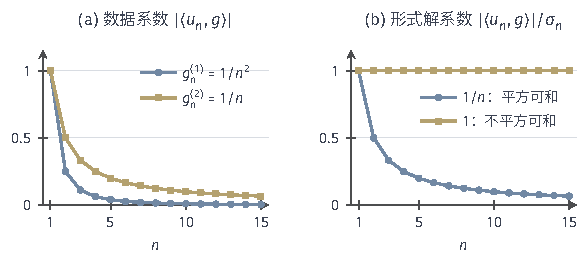
\includegraphics[width=99.6mm]{figures/02-abstract-mathematics/03-function-spaces/tikz/c3-picard-coefficients/figure.pdf}
  \caption{$\ell^2$上$A(x_n)=(x_n/n)$的Picard条件。(a)两组数据的系数$1/n^2$与$1/n$，都平方可和，都与$\ker A^*=\{0\}$正交。(b)除以奇异值$\sigma_n=1/n$后的形式解系数：前者为$1/n$，平方可和，方程可解；后者恒为$1$，不平方可和，方程无解。}
  \label{fig:opeq-picard-coefficients}
\end{figure}

函数空间中有同样的现象。在$L^2(0,1)$上考虑累积积分
\[
  (Vf)(x)=\int_0^xf(t)\,\mathrm dt .
\]
由Fubini定理交换积分次序，
\begin{equation*}
\langle g,Vf\rangle=\int_0^1\overline{g(x)}\int_0^xf(t)\,\mathrm dt\,\mathrm dx=\int_0^1\Bigl(\int_t^1\overline{g(x)}\,\mathrm dx\Bigr)f(t)\,\mathrm dt,
\end{equation*}
所以伴随为$(V^*g)(t)=\int_t^1g(x)\,\mathrm dx$。若$Vf=0$，则$f$在每个区间$[0,x]$上的积分为零，从而在每个子区间上的积分为零，$f=0$几乎处处；同理$V^*$也是单射。于是$\ker V=\ker V^*=\{0\}$，$V$的像在$L^2(0,1)$中稠密。

$V$的奇异系统可以直接写出。记$\omega_k=(k-\frac12)\pi$，$k=1,2,\ldots$，令
\[
  v_k(x)=\sqrt2\cos\omega_kx,\qquad u_k(x)=\sqrt2\sin\omega_kx,\qquad \sigma_k=\frac1{\omega_k}.
\]
直接积分得$Vv_k=\sqrt2\sin(\omega_kx)/\omega_k=\sigma_ku_k$；又由$\cos\omega_k=0$，$V^*u_k=\sqrt2\bigl(\cos\omega_kx-\cos\omega_k\bigr)/\omega_k=\sigma_kv_k$。由$\sin2\omega_k=0$可验证$(v_k)$与$(u_k)$各自标准正交。

还要说明这些就是全部奇异方向。$V^*V$是紧自伴算子且为单射，由第~\ref{chap:operator-spectra}章的谱分解，它的非零特征方向张成整个$L^2(0,1)$。若$V^*Vf=\mu f$，$\mu>0$，令$y=V^*Vf$，则$y(x)=\int_x^1\int_0^tf$，于是$y(1)=0$，$y'(x)=-\int_0^xf$，$y'(0)=0$。$f=y/\mu$连续，故$y$二阶连续可微且$y''=-f=-y/\mu$。满足$y'(0)=0$的解为$y=c\cos(x/\sqrt\mu)$，再由$y(1)=0$得$1/\sqrt\mu=\omega_k$。因此特征值为$\sigma_k^2$，每个特征空间由$v_k$张成，$(v_k)$是$L^2(0,1)$的标准正交基。

现在取数据$g=1$。由$\ker V^*=\{0\}$，它满足第一个条件。系数为
\[
  \langle u_k,1\rangle=\sqrt2\int_0^1\sin\omega_kx\,\mathrm dx=\frac{\sqrt2(1-\cos\omega_k)}{\omega_k}=\sqrt2\,\sigma_k ,
\]
形式解系数恒为$\sqrt2$，Picard条件不成立，所以$1\notin\operatorname{Ran}V$。这与直接观察一致：$Vf$总有在$0$处取零的连续代表，而常函数$1$的连续代表在$0$处取$1$，两个连续函数若几乎处处相等就处处相等。

$1$能被输出逼近，逼近的代价是输入越来越大。取$f_n=n\mathbf 1_{[0,1/n]}$，则$(Vf_n)(x)=\min\{nx,1\}$，
\[
  \lVert Vf_n-1\rVert^2=\int_0^{1/n}(1-nx)^2\,\mathrm dx=\frac1{3n}\to0,\qquad \lVert f_n\rVert^2=n\to\infty .
\]
输出误差趋于零时，产生这些输出的输入并不收敛，它们的范数无界。像的闭包里多出来的元素，正是只能这样“追到”而不能真正达到的数据。

\paragraph{Picard条件与求导}
对一般数据，$V$的Picard条件有一个熟悉的含义。设$g$有绝对连续的代表，$g(0)=0$且$g'\in L^2(0,1)$。分部积分，并利用$\cos\omega_k=0$与$g(0)=0$消去边界项：
\[
  \langle u_k,g\rangle=\Bigl[-\frac{\sqrt2\cos\omega_kx}{\omega_k}g(x)\Bigr]_0^1+\frac1{\omega_k}\int_0^1\sqrt2\cos(\omega_kx)\,g'(x)\,\mathrm dx=\sigma_k\langle v_k,g'\rangle .
\]
这里$g$取实值；复值时对实部、虚部分别计算即可。于是Picard级数等于$\sum_k\lvert\langle v_k,g'\rangle\rvert^2=\lVert g'\rVert^2<\infty$，最小范数解就是$f^\dagger=g'$。反过来，若$Vf=g$，则$g$绝对连续、$g(0)=0$且$g'=f$几乎处处。所以$\operatorname{Ran}V$恰好由这样的函数组成，求解第一类方程$Vf=g$就是对数据求导。

这个例子把前面的两个条件落到了具体的函数性质上：$g\perp\ker V^*$对所有$L^2$函数成立，几乎不提供信息；Picard条件则要求数据在$0$处的值合适并具有平方可积的导数。数据的这种正则性正是由奇异值趋于零的速度决定的，它将在第~\ref{sec:opeq-stability}节中重新出现，成为误差放大的来源。

\section{第二类算子方程}
\label{sec:opeq-second-kind}

另一类方程中，未知函数同时出现在算子里面和外面：$u$等于已知的源项加上$u$自身的一个积分平均。写成矩阵，就是$(\bm I-\lambda\bm A)\bm x=\bm b$。多出来的这个恒等项看起来不起眼，却改变了方程的全部性质。本节先在贯穿例子上比较两类方程，再分两步研究可解性：参数较小时直接构造逆，一般参数下建立Fredholm择一。

\paragraph{方程与恒等项}
设$H$为Hilbert空间，$K:H\to H$为紧算子。与第一类方程不同，这里输入和输出必须在同一个空间中，$u$与$Ku$才能相减。

\begin{definition}[第二类算子方程]
\label{def:opeq-second-kind}
给定紧算子$K:H\to H$、参数$\lambda\in\mathbb F$与$f\in H$，求$u\in H$使
\begin{equation}
  (I-\lambda K)u=f,
  \label{eq:opeq-second-kind}
\end{equation}
称为\term{第二类算子方程}（operator equation of the second kind）。若$K$是核为$k$的积分算子，方程写成
\begin{equation}
  u(x)-\lambda\int k(x,z)u(z)\,\mathrm d\mu(z)=f(x),
  \label{eq:opeq-second-kind-integral}
\end{equation}
也称为第二类积分方程。
\end{definition}

回到秩二算子$T$，它在三类方向上分别乘以$1$、$\frac13$、$0$。把$u=\alpha+\beta x+h$与$f=a+bx+r$按同样的方式分解，$h,r$都与$1,x$正交，逐方向比较系数：
\begin{equation}
  (1-\lambda)\alpha=a,\qquad
  \Bigl(1-\frac\lambda3\Bigr)\beta=b,\qquad
  h=r.
  \label{eq:opeq-rank-two-second}
\end{equation}

只要$\lambda\neq1,3$，每个$f$都给出唯一解。例如$\lambda=\frac12$时，三个方向的结果是
\[
  \alpha=2a,\qquad \beta=\frac65b,\qquad h=r.
\]
第一类方程把正交补方向压成零，信息丢失；这里$I-\lambda T$在这些方向上恰好是恒等作用，信息完好。图~\ref{fig:opeq-equation-types}把这一差别画成各方向上的乘子：蓝色的乘子有零，绿色的没有。

\begin{BookInlineFigure}
  \centering
  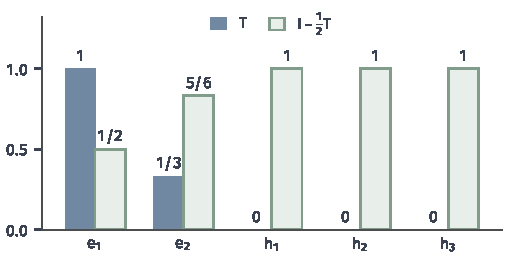
\includegraphics[width=86mm]{figures/04-spaces-measures-and-geometry/03-function-spaces/matplotlib/opeq-equation-types/figure.pdf}
  \caption{核$1+xz$（测度$\mathrm dz/2$）给出的两类方程在各正交方向上的乘子。$e_1=1$、$e_2=\sqrt3x$是特征方向，$h_1,h_2,h_3$代表与它们正交的方向（如$x^2-\frac13$）。蓝色为第一类方程的算子$T$，在正交方向上为零；绿色为第二类方程的算子$I-\frac12T$，在正交方向上恒为$1$。}
  \label{fig:opeq-equation-types}
\end{BookInlineFigure}

困难只出现在两个特殊参数上：$\lambda=1$时齐次方程$(I-T)u=0$有非零解$u=1$，$\lambda=3$时有非零解$u=x$。它们正是特征值$1$与$\frac13$的倒数。

两类方程可以使用同一个积分核，可解性却由整个算子的结构决定。第一类方程的困难来自$K$本身：零空间造成不唯一，像不够大造成无解。第二类方程只在$1/\lambda$恰为$K$的特征值时出问题。下面两个小节分别处理“$\lambda$足够小”与“$\lambda$任意”两种情形。

\subsection{Neumann级数}
\label{sec:opeq-neumann}

标量方程$(1-q)x=f$在$\lvert q\rvert<1$时有解$x=\sum_{n\geq0}q^nf$。算子方程可以照此办理，只要几何级数在算子范数下收敛。第~\ref{chap:operator-spectra}章已经用这个级数确定谱的位置；这里把它当作解方程的方法，需要的是截断之后的余项。

\begin{theorem}[Neumann级数]
\label{thm:opeq-neumann}
设$X$为Banach空间，$S\in\mathcal B(X)$且$\lVert S\rVert<1$。则$I-S$有定义在整个$X$上的有界逆，
\begin{equation}
  (I-S)^{-1}=\sum_{n=0}^{\infty}S^n,\qquad
  \lVert(I-S)^{-1}\rVert\leq\frac{1}{1-\lVert S\rVert},
  \label{eq:opeq-neumann}
\end{equation}
级数按算子范数收敛。并且部分和$P_N=\sum_{n=0}^NS^n$满足
\begin{equation}
  \bigl\lVert(I-S)^{-1}-P_N\bigr\rVert\leq\frac{\lVert S\rVert^{N+1}}{1-\lVert S\rVert}.
  \label{eq:opeq-neumann-remainder}
\end{equation}
\end{theorem}

\begin{proof}
由$\lVert S^n\rVert\leq\lVert S\rVert^n$，对$M>N$有
\[
  \lVert P_M-P_N\rVert\leq\sum_{n=N+1}^M\lVert S\rVert^n.
\]
右端是收敛几何级数的尾部，所以$(P_N)$在$\mathcal B(X)$中是Cauchy列。第~\ref{chap:linear-operators}章说明$X$完备时$\mathcal B(X)$完备，所以$P_N$收敛到某个$P$，并且
\[
  \lVert P\rVert\leq\sum_{n\geq0}\lVert S\rVert^n=\frac1{1-\lVert S\rVert}.
\]

逐项相乘时中间各项相消，部分和满足
\[
  P_N(I-S)=(I-S)P_N=I-S^{N+1}.
\]
由$\lVert S^{N+1}\rVert\leq\lVert S\rVert^{N+1}\to0$，令$N\to\infty$，得到$P(I-S)=(I-S)P=I$，所以$P$是$I-S$的有界逆。

最后，$P-P_N=\sum_{n>N}S^n$，逐项取范数并对几何级数求和，即得式~\eqref{eq:opeq-neumann-remainder}。
\end{proof}

级数$\sum_{n\geq0}S^n$称为\term{Neumann级数}（Neumann series）。取$S=\lambda K$，条件$\lVert S\rVert<1$就是$\lvert\lambda\rvert\lVert K\rVert<1$。此时第二类方程~\eqref{eq:opeq-second-kind}对每个$f$有唯一解
\begin{equation}
  u=\sum_{n=0}^\infty\lambda^nK^nf,\qquad
  \lVert u\rVert\leq\frac{\lVert f\rVert}{1-\lvert\lambda\rvert\lVert K\rVert}.
  \label{eq:opeq-neumann-solution}
\end{equation}
这一构造只用到小范数和空间的完备性，没有用到$K$的紧性。

\paragraph{截断与迭代}
实际计算只能保留有限项。记$q=\lvert\lambda\rvert\lVert K\rVert<1$，$u_N=\sum_{n=0}^{N}(\lambda K)^nf$。由式~\eqref{eq:opeq-neumann-remainder}，误差满足
\begin{equation}
  \lVert u-u_N\rVert\leq\frac{q^{N+1}}{1-q}\lVert f\rVert.
  \label{eq:opeq-neumann-truncation}
\end{equation}
误差按几何速度下降，$q$接近$1$时，同样的精度需要多得多的项。

部分和不必逐项计算$K^n$，可以递推：
\begin{equation}
  u_N=f+\lambda Ku_{N-1},\qquad u_{-1}=0.
  \label{eq:opeq-neumann-iteration}
\end{equation}
这就是不动点迭代$u\mapsto f+\lambda Ku$，也就是\BookChapterRef{chap:stationary-iterations}{卷二第11章“定常迭代法”}中步长取$1$的Richardson迭代的算子形式。这个映射满足
\[
  \lVert(f+\lambda Ku)-(f+\lambda Kw)\rVert\leq q\lVert u-w\rVert,
\]
是完备空间上的压缩映射，第~\ref{chap:metric-space-maps}章的压缩映射原理说明，从任意初值出发迭代都收敛到同一个解。

下面在秩二例子上走一遍，数据是
\[
  \lambda=\frac12,\qquad f=1+x.
\]
这时$\lVert T\rVert=1$，$q=\frac12$，由式~\eqref{eq:opeq-rank-two-second}，精确解为$u=2+\frac65x$。迭代的第一步是
\[
  u_0=1+x,\qquad
  u_1=f+\frac12Tu_0=\frac32+\frac76x.
\]

写$u_N=a_N+b_Nx$，式~\eqref{eq:opeq-neumann-iteration}给出两个系数各自的递推：
\[
  a_N=1+\frac12a_{N-1},\qquad b_N=1+\frac16b_{N-1}.
\]
解这两个递推，得到
\[
  a_N=2\bigl(1-2^{-(N+1)}\bigr),\qquad
  b_N=\frac65\bigl(1-6^{-(N+1)}\bigr).
\]
以$N=2$为例，$a_2=\frac74$，$b_2=\frac{43}{36}$。

一次多项式的范数由下式计算：
\[
  \lVert\alpha+\beta x\rVert^2=\lvert\alpha\rvert^2+\frac{\lvert\beta\rvert^2}3.
\]
代入系数的误差$\frac14$与$\frac1{180}$，$N=2$时的实际误差为
\[
  \sqrt{\Bigl(\frac14\Bigr)^2+\frac13\Bigl(\frac1{180}\Bigr)^2}\approx0.2500.
\]
由$\lVert f\rVert^2=\frac43$，式~\eqref{eq:opeq-neumann-truncation}给出的上界是$2^{-2}\cdot2/\sqrt3\approx0.2887$，只比实际误差大约$15\%$。

图~\ref{fig:opeq-neumann-convergence}显示，常数方向以$\frac12$的比率收敛，线性方向以$\frac16$的比率收敛；总误差由最慢的方向决定，这就是上界中$q$取算子范数的原因。

\begin{BookInlineFigure}
  \centering
  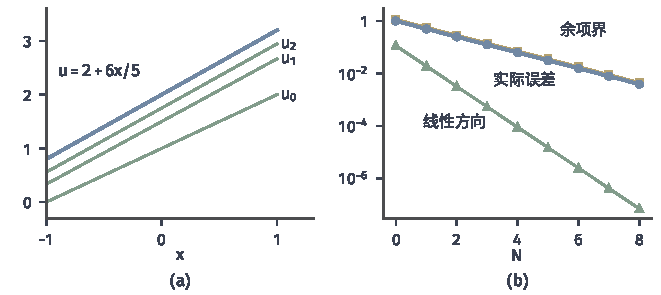
\includegraphics[width=112mm]{figures/04-spaces-measures-and-geometry/03-function-spaces/matplotlib/opeq-neumann-convergence/figure.pdf}
  \caption{$(I-\frac12T)u=1+x$的Neumann迭代。(a)绿色直线是迭代值$u_0,u_1,u_2$，蓝色直线是精确解。(b)对数纵轴上的误差：蓝色为实际误差，黄色为式~\eqref{eq:opeq-neumann-truncation}的上界，两者几乎平行；绿色为线性方向的误差，以$\frac16$的比率衰减，快于主导的常数方向。}
  \label{fig:opeq-neumann-convergence}
\end{BookInlineFigure}

\paragraph{小范数只是充分条件}
$\lvert\lambda\rvert\lVert K\rVert<1$保证可解，但远不是可解的必要条件。在秩二例子中取$\lambda=2$，常数方向的迭代系数满足$a_N=a+2a_{N-1}$，只要$a\neq0$就发散。可是$\lambda\neq1,3$，由式~\eqref{eq:opeq-rank-two-second}，方程对每个$f$仍有唯一解：
\[
  u=-a+3bx+r.
\]
取$f=1+x$，解为$u=-1+3x$。代回核对：$Tu=-1+x$，所以$u-2Tu=1+x$。方程可解与某种展开收敛是两件事。

反方向的例子是累积积分。$\lVert V\rVert=\sigma_1=2/\pi$，$\lambda=10$时$\lvert\lambda\rvert\lVert V\rVert>1$，定理的条件不成立，级数却仍然收敛。反复积分的公式是
\[
  (V^nf)(x)=\int_0^x\frac{(x-t)^{n-1}}{(n-1)!}f(t)\,\mathrm dt.
\]
由Cauchy--Schwarz不等式，$\lVert V^n\rVert\leq1/(n-1)!$，分母的增长压过任何$\lvert\lambda\rvert^n$。

所以$(I-\lambda V)u=f$对每个$\lambda$都有唯一解。取$f=1$，由$V^n1=x^n/n!$，得到
\[
  u(x)=\sum_{n=0}^\infty\frac{(\lambda x)^n}{n!}=e^{\lambda x}.
\]
$\lambda=10$时代回核对：$10Vu=e^{10x}-1$，所以$u-10Vu=1$。这与第~\ref{chap:operator-spectra}章的结论相符：$V$的谱只有$\{0\}$，没有非零特征值。要对所有参数判断可解性，需要用到$K$的紧性，这就是下一小节的内容。

\subsection{Fredholm可解条件}
\label{sec:opeq-fredholm}

先把参数分成情形。$\lambda=0$时方程就是$u=f$，总有唯一解。$\lambda\neq0$时，
\[
  I-\lambda K=-\lambda\Bigl(K-\frac1\lambda I\Bigr),
\]
所以齐次方程$(I-\lambda K)u=0$有非零解，当且仅当$1/\lambda$是$K$的特征值。

方阵有一个熟悉的事实：$\bm B\bm x=\bm 0$只有零解，当且仅当$\bm B\bm x=\bm b$对每个右端有解；若有非零解，则$\bm b$必须与$\bm B^\top$的零空间正交。下面说明，对$B=I-\lambda K$这个结论原样成立。先在紧自伴情形用特征方向看清答案，再对一般紧算子给出证明。

\paragraph{紧自伴情形的方向解释}
设$K$为紧自伴算子。为避免与参数$\lambda$混淆，记它的非零特征值为$\mu_j$。由第~\ref{chap:operator-spectra}章的谱分解，存在实数$\mu_j\neq0$与标准正交特征向量$e_j$，使每个$w\in H$写成$w=w_0+\sum_j\langle e_j,w\rangle e_j$，其中$w_0\in\ker K$；若特征值有无穷多个，则$\mu_j\to0$。把$I-\lambda K$作用在$u$上，得到
\[
  (I-\lambda K)u=u_0+\sum_j(1-\lambda\mu_j)\langle e_j,u\rangle e_j.
\]
$I-\lambda K$在零空间上是恒等作用，在第$j$个特征方向上乘以$1-\lambda\mu_j$。

若$\lambda$不等于任何$1/\mu_j$，这些乘子都不为零。又因为$\mu_j\to0$，乘子趋于$1$，只有有限个乘子离$1$较远，所以$\inf_j\lvert1-\lambda\mu_j\rvert>0$。逐方向除以乘子就得到有界逆：
\begin{equation}
  u=f_0+\sum_j\frac{\langle e_j,f\rangle}{1-\lambda\mu_j}e_j,
  \label{eq:opeq-self-adjoint-solution}
\end{equation}
其中$f_0$是$f$在$\ker K$上的分量。

若$\lambda=1/\mu_k$，乘子在$\mu_k$的特征空间上为零。这个特征空间有限维，就是齐次方程的解空间。此时方程可解，当且仅当$f$在这些方向上的系数为零，即$f\perp\ker(I-\lambda K)$；解可以加上该特征空间中的任意元素。

秩二例子中，$\lambda=1$时方程$(I-T)u=f$可解当且仅当$a=\langle1,f\rangle=0$。此时由式~\eqref{eq:opeq-rank-two-second}，第二个方程给出$\frac23\beta=b$，解为
\[
  u=c+\frac32bx+r,\qquad c\text{任意}.
\]
图~\ref{fig:opeq-fredholm-alternative}(a)画出三个乘子随$\lambda$的变化。除$\lambda=1,3$这两个参数外方程总是唯一可解，$\lambda=\frac12$与$\lambda=2$都在这个范围内，虽然只有前者满足小范数条件。

\begin{BookInlineFigure}
  \centering
  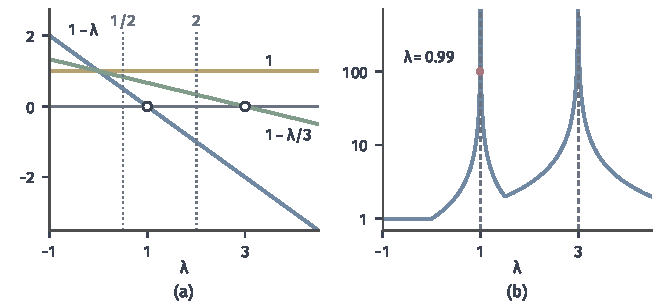
\includegraphics[width=112mm]{figures/04-spaces-measures-and-geometry/03-function-spaces/matplotlib/opeq-fredholm-alternative/figure.pdf}
  \caption{第二类方程$(I-\lambda T)u=f$对参数的依赖（核$1+xz$，测度$\mathrm dz/2$）。(a)三个方向的乘子：蓝色$1-\lambda$、绿色$1-\lambda/3$、黄色恒为$1$。空心圆处乘子为零，是例外参数；点线标出$\lambda=\frac12$（满足小范数条件）与$\lambda=2$（不满足，但仍唯一可解）。(b)逆算子的范数，对数纵轴，在两个例外参数处趋于无穷；红点为$\lambda=0.99$，范数$100$。}
  \label{fig:opeq-fredholm-alternative}
\end{BookInlineFigure}

\paragraph{Fredholm择一}
一般紧算子没有正交特征基可用，但结论的形式保持不变，只是正交条件要改用伴随方程的零空间。

\begin{theorem}[Fredholm择一]
\label{thm:opeq-fredholm}
设$H$为Hilbert空间，$K:H\to H$为紧算子，$\lambda\in\mathbb F$，$B=I-\lambda K$。则
\begin{enumerate}
  \item $\ker B$与$\ker B^*$都是有限维的，且$\dim\ker B=\dim\ker B^*$；
  \item $\operatorname{Ran}B$是闭子空间，因而$\operatorname{Ran}B=(\ker B^*)^\perp$；
  \item $\ker B=\{0\}$当且仅当$\operatorname{Ran}B=H$，此时$B^{-1}$有界。
\end{enumerate}
因此以下两种情形恰有一种成立。或者齐次方程$Bu=0$只有零解，此时对每个$f\in H$，方程$Bu=f$有唯一解，解由有界算子$B^{-1}$给出。或者齐次方程有非零解，此时$Bu=f$可解当且仅当$f\perp\ker B^*$，全部解为一个特解加上有限维子空间$\ker B$中的任意元素。
\end{theorem}

这一结论称为\term{Fredholm择一}（Fredholm alternative）。其中$B^*=I-\overline\lambda K^*$。取伴随方程$B^*w=0$的解空间的一组基$w_1,\ldots,w_r$，可解条件就是有限个等式
\begin{equation}
  \langle w_i,f\rangle=0,\qquad i=1,\ldots,r,
  \label{eq:opeq-compatibility}
\end{equation}
称为方程的\term{相容条件}（compatibility condition）。非唯一来自有限维的$\ker B$，不可解来自数据违反有限个相容条件，满足这些条件的数据都可解。

定理的关键是第二条。像的闭性由紧性事先保证，所以正交条件$f\perp\ker B^*$判断的是精确可解，而不只是$f$能否被输出逼近。上一节的对角算子$A$正好相反：每个数据都满足正交条件，但$A$的像不闭，$(1/n)$不在其中。

为什么条件要看伴随的零空间，而不是$\ker B$本身？用一个不自伴的例子说明。在$L^2(0,1)$上取秩一算子
\[
  (Ku)(x)=x\int_0^1u(z)\,\mathrm dz,
\]
并取$\lambda=2$，$B=I-2K$。

直接计算两个零空间。$u=x$满足$Ku=\frac12x$，所以$\ker B=\operatorname{span}\{x\}$。伴随是$(K^*w)(z)=\int_0^1xw(x)\,\mathrm dx$，输出总是常函数，代入$w=1$得$K^*1=\frac12$，所以$\ker B^*=\operatorname{span}\{1\}$。

把方程$u-2x\int_0^1u=f$两边在$[0,1]$上积分，左边是$\int u-2\cdot\frac12\int u=0$，所以
\[
  \int_0^1f(x)\,\mathrm dx=0
\]
是必要条件，这正是$f\perp1$，不是$f\perp x$。例如$f=2x-1$满足这个条件，全部解为$u=2x-1+cx$，而它与$x$并不正交，$\langle x,f\rangle=\frac16$。$f=1$违反条件，方程无解。

\paragraph{有限秩部分与小范数余项}
证明的想法是把紧算子拆成两部分：有限秩部分化成有限维线性方程组，余项用Neumann级数吸收。这样，无限维方程的可解性就完全由一个方阵决定。$\lambda=0$时$B=I$，结论直接成立，下面设$\lambda\neq0$。

\begin{proof}
第一步，分解。由第~\ref{chap:linear-operators}章，Hilbert空间上的紧算子能按算子范数被有限秩算子逼近。取有限秩算子$F$使$\lVert\lambda(K-F)\rVert<1$，记$C=I-\lambda(K-F)$。由定理~\ref{thm:opeq-neumann}，$C$有有界逆，于是
\[
  B=C-\lambda F=C(I-G),\qquad G=\lambda C^{-1}F.
\]

$G$仍是有限秩的有界算子。取$\operatorname{Ran}G$的一组基$b_1,\ldots,b_r$，则$Gu=\sum_{i=1}^r\ell_i(u)b_i$。系数$\ell_i$是有界线性泛函，因为有限维空间上的坐标泛函连续，与有界的$G$复合仍有界。由Riesz表示写成$\ell_i(u)=\langle a_i,u\rangle$，于是
\[
  Gu=\sum_{i=1}^r\langle a_i,u\rangle b_i.
\]

第二步，化为矩阵方程。令$\bm M$是$r\times r$矩阵，$\bm M_{i,j}=\langle a_i,b_j\rangle$，并记
\[
  \bm d(h)=(\langle a_1,h\rangle,\ldots,\langle a_r,h\rangle)^\top.
\]
我们断言：$(I-G)u=h$当且仅当$u=h+\sum_ic_ib_i$，其中$\bm c$满足
\[
  (\bm I-\bm M)\bm c=\bm d(h).
\]

若$(I-G)u=h$，则$u=h+Gu=h+\sum_ic_ib_i$，其中$c_i=\langle a_i,u\rangle$。把$u$的表达式代入这个内积，得到
\[
  c_i=\langle a_i,h\rangle+\sum_j\bm M_{i,j}c_j.
\]
反过来，若$\bm c$满足矩阵方程，令$u=h+\sum_jc_jb_j$，则
\[
  \langle a_i,u\rangle=\bm d(h)_i+(\bm M\bm c)_i=c_i,
\]
所以$Gu=\sum_ic_ib_i=u-h$。

第三步，像是闭的。由第二步，$h\in\operatorname{Ran}(I-G)$当且仅当$\bm d(h)\in\operatorname{Ran}(\bm I-\bm M)$。有限维子空间$\operatorname{Ran}(\bm I-\bm M)$是闭集，$\bm d$连续，所以$\operatorname{Ran}(I-G)$作为闭集的原像是闭的。$C$及其逆都连续，把闭集映成闭集，所以
\[
  \operatorname{Ran}B=C\bigl(\operatorname{Ran}(I-G)\bigr)
\]
闭。再由第~\ref{chap:linear-operators}章的关系$\overline{\operatorname{Ran}B}=(\ker B^*)^\perp$，第二条结论成立。

第四步，比较两个零空间的维数。取$h=0$，第二步说明$\bm c\mapsto\sum_ic_ib_i$是$\ker(\bm I-\bm M)$到$\ker(I-G)$的线性双射，这里用到$b_i$线性无关。$C$可逆，所以$\ker B=\ker(I-G)$，于是
\[
  \dim\ker B=\dim\ker(\bm I-\bm M).
\]

伴随一侧同样计算。由内积的共轭线性，$G^*w=\sum_i\langle b_i,w\rangle a_i$。若$w=G^*w$，令$d_i=\langle b_i,w\rangle$，则$w=\sum_jd_ja_j$，再与$b_i$作内积，得到
\[
  d_i=\sum_j\langle b_i,a_j\rangle d_j,
\]
这正是$\bm d=\bm M^{\mathsf H}\bm d$。反过来，每个满足此式的$\bm d$都给出$w=\sum_jd_ja_j\in\ker(I-G^*)$，且$w$确定$\bm d$，所以两个解空间线性同构。

又$B^*=(I-G^*)C^*$，$C^*$可逆，所以$\ker B^*$与$\ker(I-G^*)$维数相同。方阵与其共轭转置的秩相等，于是
\[
  \dim\ker B^*=\dim\ker(\bm I-\bm M^{\mathsf H})=\dim\ker(\bm I-\bm M)=\dim\ker B.
\]
这个公共的维数不超过$r$，第一条结论成立。

第五步，单射与满射等价。若$\ker B=\{0\}$，由第四步$\ker B^*=\{0\}$，再由第二条，$\operatorname{Ran}B=H$。反之，若$\operatorname{Ran}B=H$，则$\ker B^*=(\operatorname{Ran}B)^\perp=\{0\}$，由第四步$\ker B=\{0\}$。双射的有界算子$B$的逆有界，这由第~\ref{chap:linear-operators}章的开映射定理保证。
\end{proof}

用前面的秩一算子走一遍证明。这里$K$已是有限秩，取$F=K$，则$C=I$，$G=\lambda K$，只需一个基$b_1=x$，$a_1=\lambda\cdot1$（取实数$\lambda$），于是
\[
  \bm M=\langle a_1,b_1\rangle=\frac\lambda2,\qquad \bm d(h)=\lambda\int_0^1h.
\]
矩阵方程是一个标量方程：
\[
  \Bigl(1-\frac\lambda2\Bigr)c=\lambda\int_0^1h(x)\,\mathrm dx.
\]

$\lambda=1$时，$c=2\int h$，解为$u=h+2x\int_0^1h$。取$h=1$得$u=1+2x$，代回核对：$\int_0^1u=2$，所以$u-x\int_0^1u=1$。$\lambda=2$时，标量方程变成$0\cdot c=2\int h$，要求$\int h=0$，且$c$任意，这正是前面得到的相容条件和解的结构。

无限维方程的全部可解性就这样落在一个矩阵上，无限维的部分被可逆的$C$吸收了。这也说明了紧性的作用：若$K$不能被有限秩算子逼近，就无法这样把问题化到有限维。另一方面，定理只说明解存在并有界地依赖于数据，并不给出收敛的迭代格式，前面$\lambda=2$的例子正处于“唯一可解但Neumann级数发散”的情形。

定理的第三条也与第~\ref{chap:operator-spectra}章的结论一致：若$\mu\neq0$不是紧算子$K$的特征值，取$\lambda=1/\mu$，则$I-\lambda K$是单射，因而有有界逆，$K-\mu I=-\mu(I-\lambda K)$也有有界逆。所以紧算子的非零谱点都是特征值。这里的证明只用到有限秩逼近和Neumann级数，是这一事实的另一条论证路线。

\section{算子方程的稳定性}
\label{sec:opeq-stability}

前两节回答了解是否存在、是否唯一。实际数据总带有误差，即使方程对精确数据有唯一解，也还要问：数据改变一点，解会不会改变很多？这个问题只有在固定了输入和输出的范数之后才有确切含义，因为“一点”和“很多”都要用范数来量。本节先把三个要求并列写出，再分别考察第一类方程中的小奇异值和第二类方程中的共振参数。

\paragraph{适定问题}
设$X,Y$是赋范空间，$A:X\to Y$是有界线性算子，考虑方程$Ax=y$。按Hadamard的说法，若同时满足
\begin{enumerate}
  \item 存在：对每个$y\in Y$都有解；
  \item 唯一：解至多一个；
  \item 稳定：解连续依赖于数据，即$A^{-1}:Y\to X$连续，
\end{enumerate}
就称这个方程是\term{适定问题}（well-posed problem），否则称为\term{不适定问题}（ill-posed problem）。

三条要求相互独立，也都依赖于所取的范数。同一个求导问题，若把数据空间的范数加强到包含导数，误差放大就可能消失；所以说一个方程“不稳定”时，必须同时说明在哪对范数之下。$X,Y$都是Banach空间时，前两条已经蕴含第三条：有界双射的逆有界，这正是第~\ref{chap:linear-operators}章开映射定理的推论。因此在完备空间中，失去稳定性总是伴随着失去存在性，即像不是整个空间，甚至不闭。

\paragraph{趋于零的奇异值}
设$K:H_1\to H_2$为紧算子，并有无限多个正奇异值，$\sigma_j\to0$。在最小范数解的意义下，即使限制在可解的数据上，解也不连续依赖于数据。取数据扰动$\delta g_j=\sigma_ju_j$，则$\lVert\delta g_j\rVert=\sigma_j\to0$；它满足Picard条件，相应的最小范数解扰动为
\[
  \delta f_j=\frac{\langle u_j,\delta g_j\rangle}{\sigma_j}v_j=v_j,\qquad\lVert\delta f_j\rVert=1 .
\]
数据误差趋于零，解的误差却始终为$1$。所以映射$g\mapsto f^\dagger$在$\operatorname{Ran}K$上是无界的线性映射。

只有有限多个正奇异值时情况相反：Picard级数中各项都除以不小于$\sigma_{\min}$的数，所以$\lVert f^\dagger\rVert\leq\lVert g\rVert/\sigma_{\min}$，其中$\sigma_{\min}$是最小的正奇异值。秩二例子中$\sigma_{\min}=1/3$，误差至多放大三倍。误差放大的程度不由“算子是否可逆”这一定性性质决定，而由奇异值离零有多远决定。

\begin{theorem}[紧算子的像不闭]
\label{thm:opeq-compact-range}
设$K:H_1\to H_2$为紧算子，$\operatorname{Ran}K$是无限维的。则$\operatorname{Ran}K$在$H_2$中不闭，$K$限制在$(\ker K)^\perp$上的逆$\operatorname{Ran}K\to(\ker K)^\perp$无界。
\end{theorem}

\begin{proof}
先证逆无界。设逆有界，范数为$c$，则$\operatorname{Ran}K$中范数不超过$1$的元素都是$K$作用在$(\ker K)^\perp$中范数不超过$c$的元素上的像。$K$紧，这些像组成相对紧集，所以$\operatorname{Ran}K$中的每个有界序列都有在$H_2$中收敛的子列。但$\operatorname{Ran}K$是无限维子空间，由Gram--Schmidt过程可以在其中取一列标准正交向量，它们两两距离都是$\sqrt2$，没有收敛子列；这正是第~\ref{chap:functions-as-vectors}章所说的无限维闭球不紧。矛盾，所以逆无界。

再证像不闭。若$\operatorname{Ran}K$闭，它作为闭子空间是Hilbert空间，$K$限制在闭子空间$(\ker K)^\perp$上就是两个Hilbert空间之间的有界双射。由开映射定理，其逆有界，与上一段矛盾。
\end{proof}

结合上一节，无限秩紧算子的第一类方程三条要求全部失效：像不闭，存在性只对一个稠密而不闭的子空间成立；零空间可能非零；在像上解也不连续依赖于数据。对第一类方程，这种不适定不是例外情形，而是无限维紧算子的一般性质。

\paragraph{累积积分的误差放大}
对累积积分$V$，奇异值$\sigma_k=1/((k-\frac12)\pi)$按$1/k$衰减。取真解$f=1$，精确数据$g=Vf=x$。在数据上加入扰动$\delta u_{20}$，$\delta=0.01$，最小范数解多出$(\delta/\sigma_{20})v_{20}$，其范数为$19.5\pi\delta\approx0.61$，振幅$\sqrt2\times0.61\approx0.87$。图~\ref{fig:opeq-noise-amplification}中两条数据曲线几乎重合，解中却出现明显的快速振荡。

\begin{figure}[!htb]
  \centering
  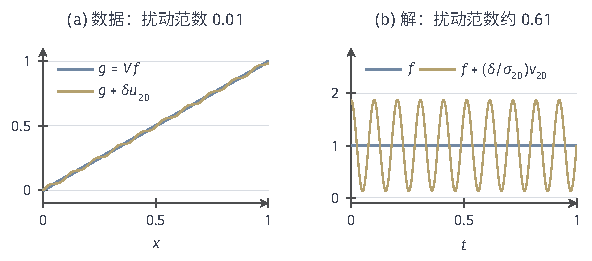
\includegraphics[width=100.2mm]{figures/02-abstract-mathematics/03-function-spaces/tikz/c3-noise-amplification/figure.pdf}
  \caption{第一类方程$Vf=g$（$(Vf)(x)=\int_0^xf$）中小奇异值放大扰动。真解$f=1$，数据$g=x$。(a)数据加上范数为$0.01$的扰动$\delta u_{20}$，与原数据几乎重合。(b)相应的最小范数解多出$(\delta/\sigma_{20})v_{20}$，振幅约$0.87$、范数约$0.61$，放大倍数$1/\sigma_{20}=19.5\pi\approx61$。}
  \label{fig:opeq-noise-amplification}
\end{figure}

这一机制与上一节“求解$Vf=g$就是求导”的结论是同一件事。$V$把快速振荡的输入平均掉，反解时必须把同样的振荡放大回去，振荡越快，放大倍数$1/\sigma_k=(k-\frac12)\pi$越大。求导在$L^2$范数下不连续：$\sin(n\pi x)/n$的范数趋于零，导数$\pi\cos(n\pi x)$的范数却不趋于零。

\paragraph{有限截断与误差的两部分}
一个自然的做法是只保留前$m$个奇异方向，令
\[
  f_m^\delta=\sum_{j\leq m}\frac{\langle u_j,g^\delta\rangle}{\sigma_j}v_j ,
\]
其中$g^\delta$是带误差的数据，$\lVert g^\delta-g\rVert\leq\delta$，$g=Kf^\dagger$为精确数据。这个截断算子有界，范数为$1/\sigma_m$。设$f_m$是用精确数据得到的截断解，则$f_m^\delta-f^\dagger=(f_m-f^\dagger)+(f_m^\delta-f_m)$。第一项是舍弃方向上的系数，第二项只含前$m$个方向上数据误差的放大；由Bessel不等式，
\begin{equation}
  \lVert f_m^\delta-f^\dagger\rVert\leq\Bigl(\sum_{j>m}\lvert\langle v_j,f^\dagger\rangle\rvert^2\Bigr)^{1/2}+\frac{\delta}{\sigma_m}.
  \label{eq:opeq-truncation-split}
\end{equation}

式~\eqref{eq:opeq-truncation-split}中，$m$增大使第一项减小、第二项增大。固定$m$时得到的是有界算子，所以截断本身是稳定的；但它求的不再是原方程的精确解，而且稳定常数$1/\sigma_m$随$m$变坏。因此不能从形式逆或某个有限截断直接推出可靠恢复：截断位置必须结合误差水平$\delta$和真解在高阶方向上的大小来选。这种选择以及用惩罚项代替硬截断的方法，属于正则化问题，可参考\BookChapterRef{chap:function-fitting-regularization}{卷五第10章“函数拟合与正则化”}；有限维中奇异值截断与条件数的关系，可参考\BookChapterRef{chap:solution-error-regularization}{卷二第14章“求解误差、正则化与方法选择”}。

\paragraph{第二类方程与共振参数}
第二类方程在$1/\lambda$不是特征值时有有界逆，因而是适定的。但“有界”并不说明界有多大。设$K$紧自伴，$\lambda$不是任何$1/\lambda_j$。由上一节的方向表示，$(I-\lambda K)^{-1}$在零空间上乘以$1$，在第$j$个特征方向上乘以$1/(1-\lambda\lambda_j)$，所以
\[
  \bigl\lVert(I-\lambda K)^{-1}\bigr\rVert=\max\Bigl\{\sup_j\frac{1}{\lvert1-\lambda\lambda_j\rvert},\ 1\Bigr\},
\]
其中$1$来自零空间上的恒等作用。$H$无限维而零空间为$\{0\}$时，特征值有无穷多个且趋于零，相应乘子的倒数趋于$1$，所以这一项不改变结果。$\lambda$靠近某个$1/\lambda_k$时，相应乘子的倒数趋于无穷，数据在$e_k$方向上的误差被放大$1/\lvert1-\lambda\lambda_k\rvert$倍。

秩二例子中，$\lVert(I-\lambda T)^{-1}\rVert=\max\{1/\lvert1-\lambda\rvert,1/\lvert1-\lambda/3\rvert,1\}$。$\lambda=0.99$时这个范数为$100$：源项在常数方向上$10^{-3}$的误差，会使解在同一方向上改变$0.1$，而其他方向上的误差几乎不被放大。与第一类方程比较，第二类方程的敏感性集中在共振参数附近的有限个方向上，远离这些参数时有统一的界；第一类方程的敏感性则来自无穷多个趋于零的奇异值，任何参数都无法消除。

\paragraph{算子的扰动}
实际计算中，算子本身也常被近似，例如用有限秩核代替原来的积分核。Neumann级数给出这时的稳定性判据。设$B=I-\lambda K$有有界逆，$E$是有界算子，且$\lVert B^{-1}\rVert\lVert E\rVert<1$。写成$B+E=B(I+B^{-1}E)$，由定理~\ref{thm:opeq-neumann}，$I+B^{-1}E$可逆，于是$B+E$可逆且
\[
  \bigl\lVert(B+E)^{-1}\bigr\rVert\leq\frac{\lVert B^{-1}\rVert}{1-\lVert B^{-1}\rVert\lVert E\rVert}.
\]
若$K_m$是$K$的有限秩近似，取$E=-\lambda(K_m-K)$，只要$\lvert\lambda\rvert\lVert K-K_m\rVert\lVert B^{-1}\rVert<1$，近似方程就仍然唯一可解，并有可控的稳定常数。这一条件同时依赖近似误差和$\lVert B^{-1}\rVert$：参数越靠近共振值，对算子近似的精度要求越高。

对第一类方程，同样的论证无法进行，因为$K$本身没有有界逆可以作为起点。这再次说明两类方程的区别来自恒等项的结构：恒等项提供了一个可逆的主部，紧算子只是对它的扰动；第一类方程中紧算子就是全部，它的逆的不连续性无法通过细化近似消除。

\section{本章小结}
\label{sec:opeq-summary}

本章开头问了三件事：给定输出能否由某个输入产生，输入是否唯一，数据误差会怎样影响解。对第一类方程$Kf=g$，前两个问题分别由像和零空间回答：有解当且仅当$g\in\operatorname{Ran}K$，解集是一个特解加上$\ker K$。紧算子的奇异系统把这两个条件写成系数条件。$g\perp\ker K^*$只说明$g$落在像的闭包里，还要求Picard条件$\sum_j\lvert\langle u_j,g\rangle\rvert^2/\sigma_j^2<\infty$，形式逆系数才拼成输入空间的元素；此时最小范数解$f^\dagger$是全部解中与零空间正交的那一个。累积积分$V$把这些条件落到具体函数上：常函数$1$能被输出任意逼近却不在像中，像中的数据恰是在$0$处取零且导数平方可积的函数，解就是导数。

第二类方程$(I-\lambda K)u=f$多了一个恒等项，在$K$看不见的方向上保留了信息。$\lvert\lambda\rvert\lVert K\rVert<1$时，Neumann级数直接给出有界逆，截断余项按$\lvert\lambda\rvert\lVert K\rVert$的幂几何下降；这一条件只是充分的，秩二例子中$\lambda=2$时级数发散而方程唯一可解。对一般参数，Fredholm择一说明：齐次方程只有零解时方程对一切数据唯一可解且逆有界；否则零空间有限维，可解性由有限个相容条件$\langle w_i,f\rangle=0$决定，其中$w_i$张成伴随方程的零空间。紧性使$I-\lambda K$的像闭，这是第二类方程与第一类方程的根本差别。

关于稳定性，适定性要求存在、唯一和连续依赖三条同时成立，并且依赖所取的范数。无限秩紧算子的像不闭，在像上求逆无界：数据扰动$\sigma_ju_j$趋于零，解的扰动始终为单位长度，累积积分中这就是求导的不稳定。截断到前$m$个奇异方向得到有界的近似逆，误差分为舍弃方向上的偏差和至多$\delta/\sigma_m$的噪声放大两部分，所以形式逆和固定截断都不能直接当作可靠恢复。第二类方程远离共振参数时是适定的，敏感性只在$\lambda$接近某个$1/\lambda_k$时出现，并集中在有限个方向上；在这种情形下，算子的小扰动也可以由Neumann级数控制。

本章只确定了方程何时可解、解怎样依赖数据。怎样根据误差水平选择截断位置或惩罚强度，怎样设计求解算法并比较偏差与误差放大，由卷五的正则化与函数拟合承担。下一章转向另一类有限表示问题：不是从输出反推输入，而是用有限个简单函数去接近给定的目标函数，并比较不同表示预算下的最佳误差。


\chapter{函数逼近}
\label{chap:function-approximation}

第~\ref{chap:functions-as-vectors}章把函数看成很长的向量$[\ldots,a_1,a_2,\ldots]$，每个输入占一个分量。计算机却只能存放有限个数，所以实际处理的总是这个长向量的一个低维替身。怎样选替身，替身离原来的函数有多远，就是本章的问题。

有限维的情形我们已经熟悉。在$\mathbb R^3$中，用$xy$平面上的点代替向量$v=(3,4,1)$，最近的点是垂足$(3,4,0)$，误差是
\[
 \lVert(3,4,1)-(3,4,0)\rVert_2=1 .
\]
三个数被压缩成两个，代价正好是被丢掉的那个分量。函数逼近做的是同一件事：候选的“平面”换成多项式、阶梯函数或若干基函数张成的子空间，“垂足”换成候选集合中离目标最近的元素。

这个图景有三个要素：要逼近的目标，量距离的尺子（范数），以及允许使用的低维候选集合。本章沿着三个问题展开。候选集合不断增大时，误差能否趋于零？只给定预算时，最小误差是多少，又怎样随预算下降？同样的预算下，选哪种候选集合最合适？

第~\ref{sec:fapprox-integrable}节回答第一个问题：在$L^p$中，简单函数、连续函数和光滑函数都能以任意精度逼近给定的可积函数，但结论依赖测度、指数$p$，在$L^\infty$中会失效。第~\ref{sec:fapprox-error}节加入预算，用点到集合的距离定义最佳误差，并用Fourier截断说明“丢掉坐标”的代价可以精确算出。

后三节比较三种选择低维替身的方式。第~\ref{sec:fapprox-fixed-subspaces}节在看到目标之前就固定子空间，类似于事先选定一张投影平面。第~\ref{sec:fapprox-best-n-term}节固定坐标轴，却按目标挑选保留哪几个坐标。第~\ref{sec:fapprox-adaptive}节让分点随目标移动，相当于连坐标轴也按目标调整。贯穿的例子是折线$f_*(x)=\lvert x-\frac12\rvert$、平方根$\sqrt x$以及在$3/4$处跳跃的阶梯函数。

有限维的直觉在两处要修正。无限维中任何有限维子空间都离整个空间很远，单位球不紧，所以单个函数的误差趋于零，并不意味着一类函数有共同的速率。不同范数也不再等价，同一个近似用不同的尺子量，结论可以完全不同。

本章只建立误差的定义、构造与基本估计。用导数、尺度或点值刻画目标的正则性，从而给出更精确的误差界，分别由第~\ref{chap:sobolev-spaces}章、第~\ref{chap:besov-spaces}章和第~\ref{chap:rkhs}章承担；从带误差的数据中拟合函数属于卷五。

\section{可积函数的逼近}
\label{sec:fapprox-integrable}

有限维中有一个基本事实：有理分量的向量在$\mathbb R^n$中稠密，任何向量都能被它们以任意精度接近。可积函数这种“无限长的向量”可能处处不连续，也可能无界，我们希望知道它能否被结构简单的函数接近。这样，许多论证就可以先对简单函数验证，再推广到一般函数。

用第~\ref{chap:topological-spaces}章的语言，这是在问某个函数族在$L^p$中是否稠密，能否取到可数的稠密族。第~\ref{chap:metric-spaces}章的距离和点列判据，把问题化为构造一列误差趋于零的近似。本节依次使用简单函数、连续函数和光滑函数，每一步都核对所用的测度、指数$p$与范数。

\subsection{简单函数逼近}
\label{sec:fapprox-simple}

只取有限多个值的可测函数称为简单函数，可以写成
\[
 s=\sum_{i=1}^kc_i\mathbf 1_{A_i},\qquad A_i\ \text{可测},\quad c_i\in\mathbb K .
\]
用向量的话说，这是分量只有有限种不同取值的向量，就像把一个长向量的每个分量四舍五入到有限个档位。第~\ref{chap:measure}章已经用取值分层构造了逐点收敛的简单函数列，这里要问的是：误差用$L^p$范数衡量时，它是否也趋于零。

\paragraph{截断与取值分层}
对非负函数，把取值范围按二进分层，每层取下端点，再把过大的值截断。设$f\geq0$可测，令
\begin{equation}
 s_n=\min\bigl\{n,\ 2^{-n}\lfloor2^nf\rfloor\bigr\},\qquad n=1,2,\ldots .
 \label{eq:fapprox-dyadic-simple}
\end{equation}
这里做了两件事：$\lfloor2^nf\rfloor/2^n$相当于把分量舍入到间距为$2^{-n}$的档位，取$\min$相当于把超过$n$的大分量压到$n$。

在$f$落入$[j2^{-n},(j+1)2^{-n})$的集合上，$s_n$取值$j2^{-n}$；在$f\geq n$的集合上，$s_n$取值$n$。所以$s_n$只取有限多个值。同时，每一点都有
\[
 0\leq s_n\leq f,
\]
并且在$f<n$处有
\[
 0\leq f-s_n<2^{-n}.
\]
$f$有限的点上，$n$足够大后都落在第二种情形，所以$s_n\to f$逐点成立。

\begin{theorem}[简单函数逼近$L^p$函数]
\label{thm:fapprox-simple-dense}
设$(X,\mathcal A,\mu)$为测度空间，$1\leq p<\infty$，$f\in L^p(\mu)$。则存在一列简单函数$s_n=\sum_ic_{n,i}\mathbf 1_{A_{n,i}}$，其中每个$\mu(A_{n,i})<\infty$，使$\lVert f-s_n\rVert_p\to0$。
\end{theorem}

\begin{proof}
先设$f\geq0$，取式~\eqref{eq:fapprox-dyadic-simple}中的$s_n$。$f\in L^p$说明$f$几乎处处有限，于是$\lvert f-s_n\rvert^p\to0$几乎处处成立。又由$0\leq s_n\leq f$，
\[
 \lvert f-s_n\rvert^p\leq f^p ,
\]
右端可积，控制收敛定理给出$\lVert f-s_n\rVert_p\to0$。

再看取值集合的测度。$n\geq1$时，$s_n$的非零取值都不小于$2^{-n}$，所以$\{s_n\neq0\}\subseteq\{f\geq2^{-n}\}$。由Chebyshev不等式，
\[
 \mu(\{s_n\neq0\})\leq\mu(\{f\geq2^{-n}\})\leq2^{np}\lVert f\rVert_p^p<\infty ,
\]
每个非零取值所在的集合测度都有限。

一般的实值$f$写成$f=f^+-f^-$，复值$f$再分实部与虚部。每一部分分别按上面逼近，组合后的误差由三角不等式控制，取值集合仍测度有限。
\end{proof}

这里$p<\infty$用了两次：控制收敛需要$f^p$可积，有限测度的支撑来自Chebyshev不等式。结论只说明简单函数在$L^p(\mu)$中稠密，并没有给出可数的稠密族，因为可测集$A_{n,i}$可以有不可数多种选法。

\begin{example}[两部分误差的大小]
取$(0,1]$上的$f(x)=x^{-1/3}$，$p=2$。它无界，但$\int_0^1x^{-2/3}\,\mathrm dx=3$，所以$f\in L^2$。我们把误差分成被截断的部分和分层舍入的部分分别计算。

$f\geq n$等价于$x\leq n^{-3}$。在这一段上$s_n=n$，平方误差是
\[
 \int_0^{n^{-3}}\bigl(x^{-1/3}-n\bigr)^2\,\mathrm dx
 =\Bigl[3x^{1/3}-3nx^{2/3}+n^2x\Bigr]_0^{n^{-3}}.
\]
代入上限，三项依次是$3/n$、$-3/n$、$1/n$，所以
\[
 \int_0^{n^{-3}}\bigl(x^{-1/3}-n\bigr)^2\,\mathrm dx=\frac1n .
\]

在其余部分，逐点误差小于$2^{-n}$，区间长度不超过$1$，平方误差不超过$4^{-n}$。合起来，
\[
 \lVert f-s_n\rVert_2^2\leq\frac1n+4^{-n}.
\]
$n=2$时右端是$0.5+0.0625$，$n=10$时约为$0.1$。舍入误差按指数下降，真正慢的是截断带来的误差。

若把$p=2$换成$p=3$，则$\int_0^1x^{-1}\,\mathrm dx=\infty$，$f$不属于$L^3$，定理不适用。此时被截断部分的三次积分也发散，误差始终是无穷大。
\end{example}

\paragraph{Lebesgue区域上的可数逼近族}
$\mathbb R^n$中用有理分量得到可数稠密集。在欧氏空间的函数上，同样的想法分两步：可测集用矩形逼近，矩形和系数都只取有理数。设$\Omega\subseteq\mathbb R^d$可测，取Lebesgue测度$\lambda$。称各边端点都是有理数的矩形$R=\prod_{i=1}^d[a_i,b_i)$为有理矩形，令$\mathcal D$为全体有限和
\[
 \sum_{i=1}^kc_i\mathbf 1_{R_i\cap\Omega},\qquad R_i\ \text{为有理矩形},\quad \operatorname{Re}c_i,\operatorname{Im}c_i\in\mathbb Q .
\]
有理矩形只有可数多个，系数也只有可数多种，所以$\mathcal D$可数。

\begin{theorem}[$L^p(\Omega)$的可数稠密族]
\label{thm:fapprox-separable}
在上述记号下，设$1\leq p<\infty$，则$\mathcal D$在$L^p(\Omega)$中稠密，因而$L^p(\Omega)$可分。
\end{theorem}

\begin{proof}
先化简目标。由定理~\ref{thm:fapprox-simple-dense}和三角不等式，只需逼近有限测度可测集$A\subseteq\Omega$的示性函数，系数换成有理复数只带来任意小的误差。对有理矩形的有限并$U$，有
\[
 \lVert\mathbf 1_A-\mathbf 1_{U\cap\Omega}\rVert_p^p=\lambda\bigl(A\mathbin{\triangle}(U\cap\Omega)\bigr)\leq\lambda(A\mathbin{\triangle}U),
\]
所以只需对任意$\varepsilon>0$，找到$U$使$\lambda(A\mathbin{\triangle}U)$小于$3\varepsilon$。

第一步，用可数个矩形覆盖$A$。由Lebesgue测度的定义（第~\ref{chap:measure}章），存在矩形$R_1,R_2,\ldots$覆盖$A$，并且$\sum_i\lambda(R_i)<\lambda(A)+\varepsilon$。于是
\[
 \lambda\Bigl(\bigcup_iR_i\setminus A\Bigr)<\varepsilon .
\]

第二步，截成有限个。级数收敛，取$N$使$\sum_{i>N}\lambda(R_i)<\varepsilon$，令$U_0=\bigcup_{i\leq N}R_i$。由$A\setminus U_0\subseteq\bigcup_{i>N}R_i$，$\lambda(A\setminus U_0)<\varepsilon$。又$U_0\setminus A\subseteq\bigcup_iR_i\setminus A$，合起来
\[
 \lambda(A\mathbin{\triangle}U_0)<2\varepsilon .
\]

第三步，把端点换成有理数。把每个$R_i$（$i\leq N$）放大成有理矩形$R_i'\supseteq R_i$，使$\lambda(R_i'\setminus R_i)<\varepsilon/N$，这只需把各端点向外移到足够近的有理数。令$U=\bigcup_{i\leq N}R_i'$，则$\lambda(U\setminus U_0)<\varepsilon$，所以
\[
 \lambda(A\mathbin{\triangle}U)<3\varepsilon .
\]
最后，有限个有理矩形的并可以用所有端点坐标切成有限个两两不交的有理矩形，因此$\mathbf 1_{U\cap\Omega}$属于$\mathcal D$。
\end{proof}

\paragraph{一般测度空间的条件}
上面的证明只用到一点：存在可数个有限测度集组成的族，使每个有限测度可测集都能用其中有限个的并按测度逼近。一般测度空间中这需要另外核对。

反例是不可数集$I$上的计数测度，此时$L^p$就是$\ell^p(I)$。这个“向量”有不可数个分量，单点示性函数$\mathbf 1_{\{i\}}$是坐标向量，两两距离为$2^{1/p}$。以它们为中心、半径$2^{1/p}/2$的开球两两不交且有不可数个，而稠密子集必须在每个球中都有元素，所以不存在可数稠密子集。

\paragraph{有界函数与本质上确界}
$p=\infty$时情况又不同。$L^\infty$范数相当于取向量各分量绝对值的最大值，这把尺子不允许任何一段上的误差被平均掉。在$L^\infty[0,1]$中取$f_t=\mathbf 1_{[0,t]}$，$0<t<1$。对$s<t$，差$f_t-f_s=\mathbf 1_{(s,t]}$在正测度集上等于$1$，所以
\[
 \lVert f_t-f_s\rVert_\infty=1 .
\]
半径$1/2$的球$\{g:\lVert g-f_t\rVert_\infty<1/2\}$两两不交，共有不可数个，同样的论证说明$L^\infty[0,1]$没有可数稠密子集。

但简单函数在$L^\infty$中仍然稠密。设$f$是实值本质有界函数，取一个满足$\lvert f\rvert\leq M$处处成立的代表。取$n\geq M$，对$f^+$与$f^-$分别作式~\eqref{eq:fapprox-dyadic-simple}的分层，组合后得到$s_n$，于是
\[
 \lVert f-s_n\rVert_\infty\leq2^{-n}.
\]
复值时分实部与虚部处理。

这两个结论并不矛盾。这里的简单函数，其取值集合是$f$的水平集，可以有不可数多种，无法取成可数族；可数的有理矩形虽然能按测度逼近这些集合，却控制不了本质上确界：把集合修改一小块，$L^\infty$误差仍可能是$1$。

\subsection{光滑函数逼近}
\label{sec:fapprox-smooth}

简单函数一般不连续。许多论证希望先对连续甚至光滑的函数推导，例如把导数移到另一个函数上，再推广到一般函数。本小节在欧氏开集$\Omega\subseteq\mathbb R^d$上取Lebesgue测度，分三步建立这种逼近：先用集合的开紧逼近得到连续函数，再证明平移在$L^p$中连续，最后用第~\ref{chap:smoothing-weak-derivatives}章的卷积磨光得到光滑函数。

\paragraph{紧支撑连续函数}
记$C_c(\Omega)$为$\Omega$上支撑为紧集的连续函数。第~\ref{chap:smoothing-weak-derivatives}章由矩形覆盖推出了Lebesgue测度的正则性：对有限测度可测集$A\subseteq\Omega$和$\varepsilon>0$，存在紧集$K$与开集$U$，使$K\subseteq A\subseteq U\subseteq\Omega$且$\lambda(U\setminus K)<\varepsilon$。于是示性函数$\mathbf 1_A$的棱角可以夹在$K$与$U$之间用一个连续的“斜坡”磨掉。

\begin{theorem}[紧支撑连续函数逼近$L^p$函数]
\label{thm:fapprox-cc-dense}
设$\Omega\subseteq\mathbb R^d$为开集，$1\leq p<\infty$，则$C_c(\Omega)$在$L^p(\Omega)$中稠密。
\end{theorem}

\begin{proof}
由定理~\ref{thm:fapprox-simple-dense}，只需逼近有限测度集$A\subseteq\Omega$的示性函数。按上面的正则性取$K\subseteq A\subseteq U$，$\lambda(U\setminus K)<\varepsilon$。若$K$是空集，取$\varphi=0$，此时误差的$p$次方不超过$\lambda(U)<\varepsilon$。下设$K$非空。

为使连续函数有紧支撑，先把$U$缩小。$K$紧且含于开集$\Omega$，它到$\Omega$的补集有正距离（$\Omega=\mathbb R^d$时这一距离取为$+\infty$）。取$\delta>0$小于这个距离，令
\[
 U'=U\cap\{x:\operatorname{dist}(x,K)<\delta\}.
\]
$U'$仍是包含$K$的开集，它的闭包含于有界闭集
\[
 \{x:\operatorname{dist}(x,K)\leq\delta\}\subseteq\Omega ,
\]
因而是$\Omega$内的紧集。

定义斜坡函数
\[
 \varphi(x)=\frac{\operatorname{dist}(x,U'^c)}{\operatorname{dist}(x,U'^c)+\operatorname{dist}(x,K)} .
\]
$K$与闭集$U'^c$不交，分母处处为正，所以$\varphi$连续。它在$K$上等于$1$，在$U'$外等于$0$，取值在$[0,1]$中，支撑含于$U'$的闭包，因而$\varphi\in C_c(\Omega)$。

最后估计误差。$\mathbf 1_A$与$\varphi$在$K$上都等于$1$，在$U$外都等于$0$，所以$\mathbf 1_A-\varphi$只在$U\setminus K$上可能非零，并且绝对值不超过$1$。于是
\[
 \lVert\mathbf 1_A-\varphi\rVert_p^p\leq\lambda(U\setminus K)<\varepsilon .
\]
\end{proof}

\paragraph{平移的$L^p$连续性}
磨光是对附近的平移作平均，所以要先知道小平移在$L^p$范数下改变函数多少。对长向量来说，平移就是把所有分量的下标错开一位。记$(\tau_hf)(x)=f(x-h)$。Lebesgue测度在平移下不变，所以$\lVert\tau_hf\rVert_p=\lVert f\rVert_p$。第~\ref{chap:smoothing-weak-derivatives}章对$p=1$证明了平移的积分连续性，下面对一般有限$p$给出同样的结论。

\begin{theorem}[平移在$L^p$中连续]
\label{thm:fapprox-translation}
设$1\leq p<\infty$，$f\in L^p(\mathbb R^d)$，则$\lVert\tau_hf-f\rVert_p\to0$（$h\to0$）。
\end{theorem}

\begin{proof}
先设$g\in C_c(\mathbb R^d)$，支撑含于球$B_R$。$g$一致连续，记
\[
 \omega_g(t)=\sup_{\lvert x-y\rvert\leq t}\lvert g(x)-g(y)\rvert ,
\]
则$\omega_g(t)\to0$。对$\lvert h\rvert\leq1$，$\tau_hg-g$的支撑含于$B_{R+1}$，所以
\[
 \lVert\tau_hg-g\rVert_p^p\leq\omega_g(\lvert h\rvert)^p\,\lambda(B_{R+1})\to0 .
\]

一般地，任给$\varepsilon>0$，由定理~\ref{thm:fapprox-cc-dense}取$g\in C_c(\mathbb R^d)$使$\lVert f-g\rVert_p<\varepsilon$。三角不等式把$\tau_hf-f$分成三段：
\[
 \lVert\tau_hf-f\rVert_p\leq\lVert\tau_h(f-g)\rVert_p+\lVert\tau_hg-g\rVert_p+\lVert g-f\rVert_p .
\]
由平移不变性，第一项等于$\lVert f-g\rVert_p<\varepsilon$；第三项也小于$\varepsilon$。于是
\[
 \lVert\tau_hf-f\rVert_p<2\varepsilon+\lVert\tau_hg-g\rVert_p ,
\]
最后一项在$h$充分小时小于$\varepsilon$。
\end{proof}

$p=\infty$时结论不成立。在$\mathbb R$上取$f=\mathbf 1_{[0,1/2]}$。对$0<\lvert h\rvert<1/2$，$\tau_hf-f$在两个长为$\lvert h\rvert$的区间上取值$\pm1$，所以
\[
 \lVert\tau_hf-f\rVert_\infty=1 .
\]
积分范数允许误差集中在测度很小的集合上，本质上确界不允许。

\paragraph{磨光的$L^p$收敛}
取第~\ref{chap:smoothing-weak-derivatives}章的磨光核：$\rho$光滑、非负、积分为$1$、支撑于单位闭球，缩放后记为
\[
 \rho_\varepsilon(x)=\varepsilon^{-d}\rho(x/\varepsilon).
\]
那里证明了$f_\varepsilon=\rho_\varepsilon*f$光滑，并在$L^1$意义下局部逼近$f$。用向量的话说，$f_\varepsilon$是对相邻分量做加权滑动平均；下面在全空间上证明$L^p$收敛，误差由平移误差控制。

\begin{theorem}[磨光在$L^p$中收敛]
\label{thm:fapprox-mollifier}
设$1\leq p<\infty$，$f\in L^p(\mathbb R^d)$，$f_\varepsilon=\rho_\varepsilon*f$。则
\begin{equation}
 \lVert f_\varepsilon-f\rVert_p\leq\sup_{\lvert h\rvert\leq\varepsilon}\lVert\tau_hf-f\rVert_p\to0\qquad(\varepsilon\to0).
 \label{eq:fapprox-mollifier-error}
\end{equation}
\end{theorem}

\begin{proof}
由$\int\rho_\varepsilon=1$，可以把$f(x)$写进平均里：
\[
 f_\varepsilon(x)-f(x)=\int\rho_\varepsilon(h)\bigl(f(x-h)-f(x)\bigr)\,\mathrm dh .
\]

$p>1$时记$q=p/(p-1)$，把被积函数写成$\rho_\varepsilon^{1/q}\cdot\rho_\varepsilon^{1/p}\lvert f(x-h)-f(x)\rvert$。由Hölder不等式与$\int\rho_\varepsilon=1$，
\[
 \lvert f_\varepsilon(x)-f(x)\rvert^p\leq\int\rho_\varepsilon(h)\,\lvert f(x-h)-f(x)\rvert^p\,\mathrm dh .
\]
$p=1$时这就是绝对值不等式。

被积函数非负可测，对$x$积分并由Tonelli定理交换积分次序，
\[
 \lVert f_\varepsilon-f\rVert_p^p\leq\int\rho_\varepsilon(h)\,\lVert\tau_hf-f\rVert_p^p\,\mathrm dh .
\]
$\rho_\varepsilon$支撑于半径$\varepsilon$的闭球且积分为$1$，所以右端是$\lVert\tau_hf-f\rVert_p^p$的加权平均，不超过它在$\lvert h\rvert\leq\varepsilon$上的上确界。由定理~\ref{thm:fapprox-translation}，这一上确界随$\varepsilon\to0$趋于零。
\end{proof}

跳跃函数最能说明指数$p$的作用。取$\mathbb R$上的$f=\mathbf 1_{[0,1/2]}$，当$\varepsilon\leq1/4$时，$f_\varepsilon-f$只集中在两个跳跃点两侧宽$\varepsilon$的带内。记$T(u)=\int_u^1\rho(v)\,\mathrm dv$，代换$x=\varepsilon u$后，两个跳跃点各贡献两段相同的积分，得到
\[
 \lVert f_\varepsilon-f\rVert_p^p=4\varepsilon\int_0^1T(u)^p\,\mathrm du .
\]

所以$L^p$误差按$\varepsilon^{1/p}$下降：$p=1$时是一阶，$p=2$时是$\varepsilon^{1/2}$。$p$越大，指数$1/p$越小。到$p=\infty$，指数变成零，而跳跃点处$f_\varepsilon$的值恒为$1/2$，误差$1/2$不再变化。图~\ref{fig:fapprox-mollifier-norms}把这件事画了出来：曲线明显向跳跃靠拢，$L^1$与$L^2$的误差都在下降，一致误差却保持不动。

\begin{BookInlineFigure}
  \centering
  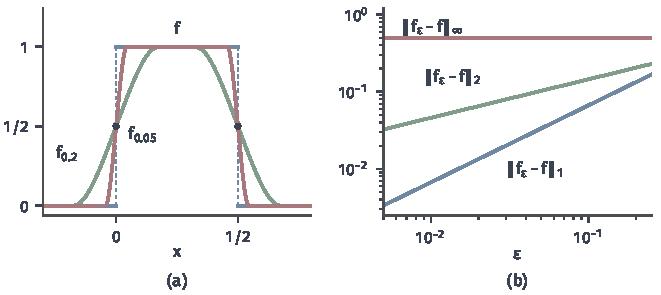
\includegraphics[width=112mm]{figures/04-spaces-measures-and-geometry/03-function-spaces/matplotlib/fapprox-mollifier-norms/figure.pdf}
  \caption{跳跃函数的磨光。(a)$f=\mathbf 1_{[0,1/2]}$（蓝）与$\varepsilon=0.2$（绿）、$\varepsilon=0.05$（红）的磨光；两个黑点标出无论$\varepsilon$多小，$f_\varepsilon$在跳跃点都等于$1/2$。(b)三种范数下的误差随$\varepsilon$的变化，双对数坐标：$L^1$误差为$2m_1\varepsilon$（$m_1\approx0.3345$），$L^2$误差正比于$\varepsilon^{1/2}$，$L^\infty$误差恒为$1/2$。}
  \label{fig:fapprox-mollifier-norms}
\end{BookInlineFigure}

\paragraph{光滑紧支撑函数与局部逼近}
两步合起来就得到光滑函数的逼近。设$f\in L^p(\Omega)$，$1\leq p<\infty$，$\varepsilon_0>0$。由定理~\ref{thm:fapprox-cc-dense}取$g\in C_c(\Omega)$使$\lVert f-g\rVert_p<\varepsilon_0$，把$g$在$\Omega$外延拓为零。

$\rho_\varepsilon*g$光滑，支撑含于$\operatorname{supp}g$的$\varepsilon$邻域。取$\varepsilon$小于$\operatorname{supp}g$到$\Omega^c$的距离，它就属于$C_c^\infty(\Omega)$。由定理~\ref{thm:fapprox-mollifier}，再取$\varepsilon$足够小，使$\lVert\rho_\varepsilon*g-g\rVert_p<\varepsilon_0$。所以$C_c^\infty(\Omega)$在$L^p(\Omega)$（$1\leq p<\infty$）中稠密。

只在局部可积的函数也有局部版本，办法是先截断。设$f\in L^p_{\mathrm{loc}}(\Omega)$，即在每个紧集上$p$次可积，$K\subset\Omega$紧。取$\delta>0$使闭邻域
\[
 K_\delta=\{x:\operatorname{dist}(x,K)\leq\delta\}
\]
含于$\Omega$，令$F=f\mathbf 1_{K_\delta}$，则$F\in L^p(\mathbb R^d)$。

对$\varepsilon<\delta$和$x\in K$，$\rho_\varepsilon(x-\cdot)$的支撑落在$K_\delta$内，所以$(\rho_\varepsilon*F)(x)=f_\varepsilon(x)$。由定理~\ref{thm:fapprox-mollifier}，
\[
 \int_K\lvert f_\varepsilon-f\rvert^p\,\mathrm dx\leq\lVert\rho_\varepsilon*F-F\rVert_p^p\to0 .
\]
截断把局部问题化为全空间问题，代价是结论只在远离边界的紧集上成立。

\paragraph{$L^\infty$中的失效}
连续函数在$L^\infty$中不稠密，光滑函数更是如此。在$(0,1)$上取$f=\mathbf 1_{(0,1/2]}$。设$g$连续且$\lVert g-f\rVert_\infty=r$，则下面两个不等式都几乎处处成立：
\[
 g\geq1-r\ \text{在}\ (0,1/2)\ \text{上},\qquad g\leq r\ \text{在}\ (1/2,1)\ \text{上}.
\]
满测度集在区间中稠密，由连续性这两个不等式在相应闭区间上处处成立。取$x=1/2$，得到
\[
 1-r\leq g(1/2)\leq r ,
\]
即$r\geq1/2$。所以任何连续函数与$f$的本质上确界距离都不小于$1/2$，这正是跳跃幅度的一半。

本节的结论都是定性的：对每个精度都存在某个近似，但没有说明近似需要多少参数。简单函数要多少层、磨光宽度要多小，取决于目标函数本身，而定理没有给出任何速率。要比较不同表示的效率，必须先固定允许使用多少参数，这是下一节的任务。

\section{逼近误差}
\label{sec:fapprox-error}

上一节说“存在误差小于$\varepsilon$的近似”，却允许近似的复杂程度随$\varepsilon$任意增长。回到章首的投影图景：要谈“替身离目标多远”，先要定下目标、尺子和允许的候选集合。本节先用候选集合定义最佳可能误差，把它同具体构造得到的误差分开；再比较候选集合是否为线性子空间、尺子是否由内积给出；最后用Fourier截断，把“丢掉坐标”的代价逐项算出来。

\subsection{目标、误差与表示预算}
\label{sec:fapprox-budget}

设$X$是赋范函数空间，$f\in X$是目标。对每个预算$N$，规定一个候选集合$\mathcal A_N\subseteq X$，它包含所有“用预算$N$能写出的函数”。预算可以是线性子空间的维数，可以是展开中允许保留的项数，也可以是分段函数的段数。

要比较候选集合的好坏，最公平的度量是其中最好的那个候选能做到多好。下面的定义就是把点到集合的距离搬到函数上。

\begin{definition}[最佳逼近误差]
\label{def:fapprox-best-error}
对$f\in X$与候选集合$\mathcal A_N\subseteq X$，称
\begin{equation}
 E(f,\mathcal A_N)_X=\inf_{g\in\mathcal A_N}\lVert f-g\rVert_X
 \label{eq:fapprox-best-error}
\end{equation}
为$f$在$\mathcal A_N$中的\term{最佳逼近误差}（error of best approximation）。
\end{definition}

这就是第~\ref{chap:metric-spaces}章的点到集合的距离。由那里的序列判据，$E(f,\mathcal A_N)_X=0$当且仅当$f$属于$\mathcal A_N$的闭包。若$\mathcal A_N$随$N$递增且并集稠密，上一节的结论就可以重述为$E(f,\mathcal A_N)_X\to0$。

最佳误差是在所有候选中取下确界，不依赖任何具体的选法。某个具体构造（例如在结点处插值）得到的误差只是它的一个上界。后面要反复区分这两者。

\paragraph{三种预算}
三种常见预算给出性质不同的候选集合。次数小于$N$的多项式组成$N$维线性空间，好比$\mathbb R^n$中一张固定的$N$维平面。

给定一组标准正交基后，至多用其中$N$个基向量的线性组合组成的集合就不同了。$\mathbb R^2$中$N=1$时，它是两条坐标轴的并，不是平面也不是直线；$e_1$与$e_2$都只用一项，和$e_1+e_2$却要两项。区间上至多$N$段的分段常数函数，若分点可以任意移动，同样不对加法封闭。

后两种集合对数乘封闭，但对加法不封闭，相应的逼近称为\term{非线性逼近}（nonlinear approximation），以区别于在固定线性空间中进行的线性逼近。

\paragraph{单个函数与函数类}
有时我们要的不是某一个函数的误差，而是对一整类函数$\mathcal F$同时有效的保证。此时考虑最坏情形
\begin{equation}
 E(\mathcal F,\mathcal A_N)_X=\sup_{f\in\mathcal F}E(f,\mathcal A_N)_X .
 \label{eq:fapprox-worst-case}
\end{equation}

两者可以相差很多，这也是无限维与有限维差别最明显的地方。设$H$是可分无限维Hilbert空间，$(e_n)$为标准正交基，$V_N=\operatorname{span}\{e_1,\ldots,e_N\}$。对每个$f$，有
\[
 E(f,V_N)^2=\sum_{n>N}\lvert\langle e_n,f\rangle\rvert^2\to0 .
\]
可是对闭单位球$\mathcal F$，取$f=e_{N+1}$，它与$V_N$垂直，距离为$1$，所以
\[
 E(\mathcal F,V_N)=1\qquad\text{对每个}\ N.
\]
单个函数的误差都趋于零，整个单位球却没有共同的速率。在$\mathbb R^n$中，取$V_n$就把全空间装下了，这种现象不会发生。

要得到统一速率，函数类本身必须足够“小”。这与第~\ref{chap:function-class-covers}章的有限覆盖直接相关：若候选集合$\mathcal A$是至多$N$个函数组成的有限集，最坏误差不超过$\varepsilon$恰好说明以$\mathcal A$中各点为中心、半径为$\varepsilon$的闭球覆盖$\mathcal F$。

反过来，若$\mathcal F$能被$N$个半径为$\varepsilon$的闭球覆盖，以这些球心为$\mathcal A$，最坏误差就不超过$\varepsilon$。覆盖数因此恰好描述了用$N$个固定函数逼近整个函数类所能达到的最坏误差。

\subsection{固定空间中的最佳逼近}
\label{sec:fapprox-fixed-space}

最常见的预算是维数。取一列嵌套的有限维子空间$V_1\subseteq V_2\subseteq\cdots\subseteq X$，$\dim V_N\leq N$，研究$E(f,V_N)_X$。一个基本的问题是：下确界能否取到，也就是最近点是否存在。

\begin{theorem}[有限维子空间中最佳逼近的存在]
\label{thm:fapprox-existence}
设$X$为赋范空间，$V\subseteq X$为有限维子空间，$f\in X$。则存在$g^*\in V$使$\lVert f-g^*\rVert=E(f,V)_X$。
\end{theorem}

\begin{proof}
记$d=E(f,V)_X$，取$g_n\in V$使$\lVert f-g_n\rVert\to d$。$n$充分大时，$\lVert f-g_n\rVert\leq d+1$，于是
\[
 \lVert g_n\rVert\leq\lVert f\rVert+\lVert f-g_n\rVert\leq\lVert f\rVert+d+1 .
\]
$(g_n)$是有限维空间中的有界序列。有限维赋范空间中有界闭集是紧集，所以有子列收敛到某个$g^*\in V$。范数连续，取极限得
\[
 \lVert f-g^*\rVert=\lim_k\lVert f-g_{n_k}\rVert=d .
\]
\end{proof}

证明的关键是有限维的闭球紧。这个定理对$V$的维数有实质要求：无限维子空间中最近点可能不存在，第~\ref{chap:function-inner-product-spaces}章用完备性和平行四边形恒等式才在Hilbert空间中重新得到它。

存在不等于唯一，尺子的形状决定了最近点的个数。在$\mathbb R^2$上取最大值范数（两个分量绝对值的较大者），$V=\operatorname{span}\{(0,1)\}$，$f=(1,0)$。对候选$(0,t)$，
\[
 \lVert f-(0,t)\rVert_\infty=\max\{1,\lvert t\rvert\},
\]
对所有$\lvert t\rvert\leq1$都取到最小值$1$，最佳逼近有无穷多个。

图~\ref{fig:fapprox-nearest-point}说明了原因。以$f$为中心把球吹大，第一次碰到$V$的地方就是最近点。欧氏球是圆，碰到直线只有一点；最大值范数的球是正方形，它的一条边整个贴上了直线。

\begin{BookInlineFigure}
  \centering
  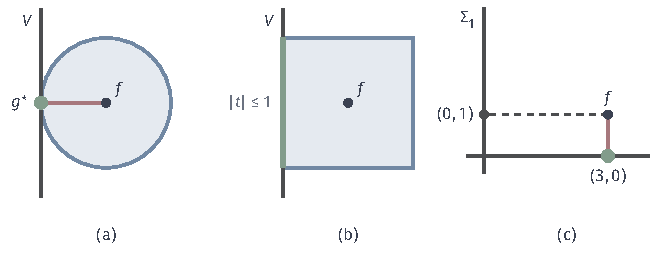
\includegraphics[width=110.882mm]{figures/04-spaces-measures-and-geometry/03-function-spaces/tikz/fapprox-nearest-point/figure.pdf}
  \caption{候选集合与尺子决定最近点。(a)$\mathbb R^2$中欧氏范数：以$f=(1,0)$为中心的圆第一次碰到直线$V$时只有一个切点$g^*$（绿）。(b)最大值范数：同样的半径下，球是正方形，整条边$\{(0,t):\lvert t\rvert\leq1\}$（绿）都是最近点。(c)候选集合$\Sigma_1$是两条坐标轴的并，并非子空间；对$f=(3,1)$，到横轴的距离$1$（红）小于到纵轴的距离$3$（虚线），最近点是$(3,0)$。}
  \label{fig:fapprox-nearest-point}
\end{BookInlineFigure}

\paragraph{Hilbert空间中的正交投影}
内积给出的尺子最好用。由第~\ref{chap:function-inner-product-spaces}章，对闭子空间$V$，正交投影$P_V$给出唯一的最佳逼近，误差满足勾股关系
\begin{equation}
 E(f,V)^2=\lVert f-P_Vf\rVert^2=\lVert f\rVert^2-\lVert P_Vf\rVert^2 .
 \label{eq:fapprox-pythagoras}
\end{equation}
若$V$有标准正交基$e_1,\ldots,e_N$，则投影公式就是把分量读出来：
\[
 P_Vf=\sum_{n\leq N}\langle e_n,f\rangle e_n .
\]
映射$f\mapsto P_Vf$是线性的，这正是后面截断误差可以逐项计算的原因。

\begin{example}[把$x^2$投影到一次函数]
在$L^2[0,1]$中，用次数不超过$1$的多项式逼近$f(x)=x^2$。这个二维子空间有标准正交基
\[
 e_1(x)=1,\qquad e_2(x)=\sqrt{12}\Bigl(x-\frac12\Bigr).
\]

读出$f$在两个方向上的分量：
\[
 \langle e_1,f\rangle=\frac13,\qquad
 \langle e_2,f\rangle=\sqrt{12}\Bigl(\frac14-\frac16\Bigr)=\frac1{\sqrt{12}}.
\]
代入投影公式，$\sqrt{12}$约去，
\[
 P_Vf(x)=\frac13+x-\frac12=x-\frac16 .
\]

误差由式~\eqref{eq:fapprox-pythagoras}得到，只需做减法，这和$\mathbb R^3$中用勾股定理求点到平面的距离一样：
\[
 E(f,V)^2=\frac15-\frac19-\frac1{12}=\frac1{180}.
\]
\end{example}

\paragraph{不同的尺子，不同的最佳近似}
在其他范数下，最佳逼近的结果和性质都会变。在$C[0,1]$中用常数作一致逼近：若$f$的最大值、最小值分别是$M,m$，则
\[
 \max_x\lvert f(x)-c\rvert=\max\{M-c,\ c-m\}.
\]
两项一增一减，取$c=(M+m)/2$时相等，最小。所以唯一的最佳常数和最佳误差是
\begin{equation}
 c^*=\frac{M+m}2,\qquad E=\frac{M-m}2 .
 \label{eq:fapprox-best-constant}
\end{equation}

对比$L^2[0,1]$中的最佳常数，它是在一维子空间$\operatorname{span}\{1\}$上的投影，等于平均值。取$f(x)=x^2$，两种尺子给出不同的答案：
\[
 c_{L^2}=\int_0^1x^2\,\mathrm dx=\frac13,\qquad c_\infty=\frac{1+0}2=\frac12 .
\]

一致逼近的最佳选择甚至不是线性的。取$f_1(x)=x$，最佳常数为$1/2$；取$f_2(x)=-x^2$，最佳常数为$-1/2$；而$f_1+f_2=x-x^2$的最大值$1/4$、最小值$0$，最佳常数为$1/8$，不等于$\frac12+(-\frac12)=0$。所以在线性空间中选近似，并不意味着“选出最佳近似”这个操作本身是线性的。第~\ref{sec:fapprox-adaptive}节的分段常数逼近要用到式~\eqref{eq:fapprox-best-constant}。

\subsection{正交展开的截断误差}
\label{sec:fapprox-fourier-truncation}

Hilbert空间中，若嵌套空间由一组标准正交基的前若干项张成，最佳误差就是被舍弃分量的平方和，和$\mathbb R^3$中丢掉第三个分量完全一样。Fourier级数是最重要的例子。本小节在$L^2(0,1)$上采用周期为$1$的基：
\[
 e_k(x)=\mathrm e^{2\pi\mathrm ikx},\qquad k\in\mathbb Z ,
\]
函数$f$在第$k$个方向上的分量是
\[
 \hat f(k)=\langle e_k,f\rangle=\int_0^1f(x)\mathrm e^{-2\pi\mathrm ikx}\,\mathrm dx .
\]
第~\ref{chap:fourier-transform}章对周期$2\pi$的基建立了完备性，作线性变量代换后，$(e_k)_{k\in\mathbb Z}$是$L^2(0,1)$的标准正交基，Parseval等式$\lVert f\rVert_2^2=\sum_k\lvert\hat f(k)\rvert^2$成立。

\paragraph{平方误差与保留维数}
保留$\lvert k\rvert\leq K$的项，令$P_Kf=\sum_{\lvert k\rvert\leq K}\hat f(k)e_k$。它是到$2K+1$维空间$\operatorname{span}\{e_k:\lvert k\rvert\leq K\}$的正交投影。由Parseval等式，
\begin{equation}
 \lVert f-P_Kf\rVert_2^2=\sum_{\lvert k\rvert>K}\lvert\hat f(k)\rvert^2 .
 \label{eq:fapprox-fourier-tail}
\end{equation}
截断误差完全由分量的衰减决定，而衰减速度反映目标的正则性。下面用一个跳跃的函数和一个连续但有折点的函数比较。

第一个是锯齿函数$f(x)=x$，周期延拓后在整数点跳跃。$k=0$时积分是$1/2$。$k\neq0$时分部积分，
\[
 \hat f(k)=\Bigl[\frac{x\,\mathrm e^{-2\pi\mathrm ikx}}{-2\pi\mathrm ik}\Bigr]_0^1+\frac1{2\pi\mathrm ik}\int_0^1\mathrm e^{-2\pi\mathrm ikx}\,\mathrm dx .
\]
第二项的积分是零，第一项的上限给出
\[
 \hat f(k)=\frac1{-2\pi\mathrm ik}=\frac{\mathrm i}{2\pi k}.
\]
代入式~\eqref{eq:fapprox-fourier-tail}，并把$\pm k$的两项合并，
\[
 \lVert f-P_Kf\rVert_2^2=\frac1{2\pi^2}\sum_{k>K}\frac1{k^2}.
\]
这个尾和约为$1/K$，误差约为$(2\pi^2K)^{-1/2}$。实际计算得$K=10$时$\lVert f-P_Kf\rVert_2=0.0694$，$K=40$时为$0.0354$。项数增至四倍，误差只减半。

第二个是三角波$f_*(x)=\lvert x-\frac12\rvert$，周期延拓后连续，只有折点。$k=0$时积分是$1/4$。$k\neq0$时作代换$x=\frac12+t$，因子$\mathrm e^{-\pi\mathrm ik}=(-1)^k$提到积分外，$\lvert t\rvert$是偶函数，只留下余弦部分：
\[
 \hat f_*(k)=2(-1)^k\int_0^{1/2}t\cos(2\pi kt)\,\mathrm dt .
\]
再分部积分一次，
\[
 \int_0^{1/2}t\cos(2\pi kt)\,\mathrm dt=\frac{(-1)^k-1}{4\pi^2k^2}.
\]
合起来，并用$(-1)^{2k}=1$，
\[
 \hat f_*(k)=\frac{1-(-1)^k}{2\pi^2k^2}\qquad(k\neq0).
\]
奇数$k$时系数为$1/(\pi^2k^2)$，偶数$k$时为零。由式~\eqref{eq:fapprox-fourier-tail}，平方误差是
\[
 \lVert f_*-P_Kf_*\rVert_2^2=\frac2{\pi^4}\sum_{\substack{k>K\\k\ \text{奇}}}\frac1{k^4}\leq\frac2{3\pi^4K^3},
\]
不等号把尾和换成积分$\int_K^\infty t^{-4}\,\mathrm dt$来控制。$K=10$时实际误差为$0.00183$。系数从$k^{-1}$变成$k^{-2}$，误差的速率就从$K^{-1/2}$提高到$K^{-3/2}$。

多变量时，同样的截断在$[0,1)^d$上使用基
\[
 e_{\bm k}(\bm x)=\mathrm e^{2\pi\mathrm i\bm k\cdot\bm x},\qquad \bm k\in\mathbb Z^d .
\]
保留$\max_i\lvert k_i\rvert\leq K$的项需要$(2K+1)^d$个系数，保留$\lvert\bm k\rvert_2\leq K$的项大约需要半径为$K$的$d$维球体积那么多个系数。例如$d=2$、$K=10$时，前者是$441$个，后者是$317$个。比较误差时必须写明预算计的是哪一种。

\paragraph{一致误差}
平方误差小不等于每一点误差都小。设系数绝对可和，即
\[
 \sum_k\lvert\hat f(k)\rvert<\infty ,
\]
则级数$\sum_k\hat f(k)e_k$一致收敛到一个连续函数$\tilde f$。$\tilde f$与$f$有相同的Fourier系数，由Parseval等式，两者几乎处处相等。这个连续代表满足
\begin{equation}
 \sup_x\bigl\lvert\tilde f(x)-P_Kf(x)\bigr\rvert\leq\sum_{\lvert k\rvert>K}\lvert\hat f(k)\rvert .
 \label{eq:fapprox-uniform-tail}
\end{equation}

三角波的系数绝对可和，右端为
\[
 \frac2{\pi^2}\sum_{\substack{k>K\\k\ \text{奇}}}\frac1{k^2}\leq\frac2{\pi^2K}.
\]
在$x=1/2$处$e_k(1/2)=(-1)^k$，所有被舍弃的项同号，所以式~\eqref{eq:fapprox-uniform-tail}在这一点取等号，一致误差恰好等于这个尾和。$K=10$时它是$0.0101$。

锯齿函数的系数不绝对可和。$f$在整数点跳跃，而$P_Kf$连续，在跳跃点两侧的误差不可能都小于跳跃幅度的一半，所以一致误差不趋于零。图~\ref{fig:fapprox-fourier-truncation}(a)中，$P_{10}f$在跳跃附近摆动，其余地方已经贴近$f$。

两种误差的控制方式不同：平方误差用平方尾和，一致误差用绝对尾和，后者要求系数衰减得更快。图~\ref{fig:fapprox-fourier-truncation}(b)显示，三角波的平方误差按$K^{-3/2}$下降，一致误差只按$K^{-1}$下降。同一个截断，换一把尺子，所需的正则性和得到的速率都不同。

\begin{BookInlineFigure}
  \centering
  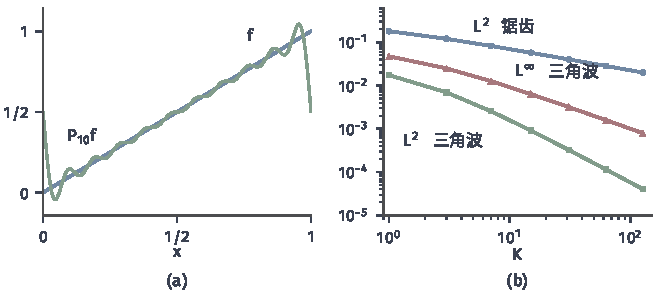
\includegraphics[width=112mm]{figures/04-spaces-measures-and-geometry/03-function-spaces/matplotlib/fapprox-fourier-truncation/figure.pdf}
  \caption{Fourier截断的误差。(a)锯齿函数$f(x)=x$（蓝）与截断$P_{10}f$（绿）。(b)误差随截断半径$K$的变化，双对数坐标，$K=1,3,7,\ldots,127$：锯齿函数的$L^2$误差按$K^{-1/2}$下降，三角波$\lvert x-\frac12\rvert$的$L^2$误差按$K^{-3/2}$下降，三角波的$L^\infty$误差按$K^{-1}$下降。}
  \label{fig:fapprox-fourier-truncation}
\end{BookInlineFigure}

\paragraph{理论截断与离散计算}
$P_Kf$中的系数是积分，实际计算时常用$M$个等距采样点上的求和代替：
\[
 \hat f_M(k)=\frac1M\sum_{j=0}^{M-1}f\Bigl(\frac jM\Bigr)\mathrm e^{-2\pi\mathrm ikj/M}.
\]
这相当于只读长向量上$M$个位置的分量，再用这$M$个数去估计频率坐标。$M$个数放不下无限多个频率坐标，必有信息被折叠到一起。

设系数绝对可和，在采样点使用连续代表$\tilde f=\sum_l\hat f(l)e_l$。把它代入上式，交换有限和与绝对收敛级数，内层出现的是几何和
\[
 \frac1M\sum_{j=0}^{M-1}\mathrm e^{2\pi\mathrm i(l-k)j/M}=
 \begin{cases}
  1,&l\equiv k\pmod M,\\
  0,&\text{其他情形}.
 \end{cases}
\]
于是
\begin{equation}
 \hat f_M(k)=\sum_{m\in\mathbb Z}\hat f(k+mM) .
 \label{eq:fapprox-aliasing}
\end{equation}
离散系数把所有与$k$模$M$同余的频率叠加在一起，这一现象称为\term{混叠}（aliasing）。

用三角波验证一下。取$M=4$，$k=1$，采样值依次是
\[
 f_*(0)=\frac12,\quad f_*\Bigl(\frac14\Bigr)=\frac14,\quad f_*\Bigl(\frac12\Bigr)=0,\quad f_*\Bigl(\frac34\Bigr)=\frac14 .
\]
指数因子依次是$1,-\mathrm i,-1,\mathrm i$，$j=1,3$两项相消，得到
\[
 \hat f_4(1)=\frac14\cdot\frac12=\frac18 .
\]

另一方面，$k+4m$取遍$\ldots,-7,-3,1,5,9,\ldots$，它们的绝对值恰好取遍所有正奇数各一次。由式~\eqref{eq:fapprox-aliasing}和$\sum_{n\ \text{奇},\,n>0}n^{-2}=\pi^2/8$，
\[
 \sum_{m\in\mathbb Z}\hat f_*(1+4m)=\frac1{\pi^2}\sum_{\substack{n>0\\n\ \text{奇}}}\frac1{n^2}=\frac18 ,
\]
两边相同。真实系数$\hat f_*(1)=1/\pi^2\approx0.1013$，被混入的高频抬高到了$0.125$。图~\ref{fig:fapprox-aliasing}(a)展示了混叠的机制，(b)展示了哪些频率被叠到一起。

\begin{BookInlineFigure}
  \centering
  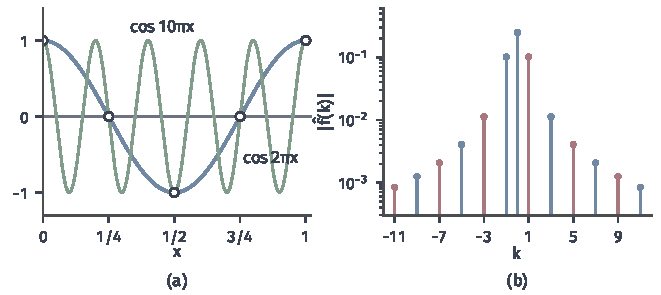
\includegraphics[width=112mm]{figures/04-spaces-measures-and-geometry/03-function-spaces/matplotlib/fapprox-aliasing/figure.pdf}
  \caption{$M=4$时的混叠。(a)$\cos2\pi x$（蓝）与$\cos10\pi x$（绿）在四个采样点$j/4$（空心圆）上取值相同，只看采样值无法区分频率$1$与$5$。(b)三角波系数的绝对值（对数纵轴）。红色频率$k\equiv1\pmod4$的系数相加，得到离散系数$\hat f_4(1)=1/8$；蓝色为其余频率。}
  \label{fig:fapprox-aliasing}
\end{BookInlineFigure}

用离散系数作截断时，误差有两个来源。设$g=\sum_{\lvert k\rvert\leq K}\hat f_M(k)e_k$，$f-g$分成互相正交的两部分：一部分在被舍弃的频率上，一部分在保留的频率上。勾股定理给出
\begin{equation}
 \lVert f-g\rVert_2^2=\sum_{\lvert k\rvert>K}\lvert\hat f(k)\rvert^2+\sum_{\lvert k\rvert\leq K}\lvert\hat f_M(k)-\hat f(k)\rvert^2 .
 \label{eq:fapprox-discrete-error}
\end{equation}

第一项是理论截断误差，只由$K$决定。第二项是离散误差，由式~\eqref{eq:fapprox-aliasing}知$\hat f_M(k)-\hat f(k)=\sum_{m\neq0}\hat f(k+mM)$，依赖采样数$M$与高频系数。两者应分别预算：增大$K$而不增大$M$，第二项不会减小；$2K+1>M$时，$M$个数据被重复计入不同的频率，增加保留项还会使离散误差变大。

\subsection{连续频带截断}
\label{sec:fapprox-band-truncation}

非周期函数没有离散频率，向量的“分量”换成了连续下标$\xi$上的$\hat f(\xi)$。相应的预算改为一段连续频带。在$L^2(\mathbb R)$上沿用第~\ref{chap:fourier-transform}章的归一化
\[
 \hat f(\xi)=\int_{\mathbb R}f(x)\mathrm e^{-2\pi\mathrm ix\xi}\,\mathrm dx ,
\]
先对$L^1\cap L^2$定义，再延拓到$L^2$。Plancherel等式是$\lVert\hat f\rVert_2=\lVert f\rVert_2$。

给定频带半宽$W>0$，令$Q_Wf$为$\hat f\mathbf 1_{[-W,W]}$的逆变换。乘以示性函数是$L^2$上的正交投影，Fourier变换是保持内积的双射，所以$Q_W$是到闭子空间
\[
 \mathcal B_W=\bigl\{g\in L^2(\mathbb R):\ \hat g=0\ \text{在}\ [-W,W]\ \text{外几乎处处成立}\bigr\}
\]
的正交投影。$\mathcal B_W$中的函数称为\term{带限函数}（band-limited function）。$Q_Wf$是$f$在$\mathcal B_W$中的最佳$L^2$逼近，由Plancherel等式，
\begin{equation}
 \lVert f-Q_Wf\rVert_2^2=\int_{\lvert\xi\rvert>W}\lvert\hat f(\xi)\rvert^2\,\mathrm d\xi .
 \label{eq:fapprox-band-tail}
\end{equation}

以Gauss函数$f(x)=\mathrm e^{-\pi x^2}$为例，$\hat f(\xi)=\mathrm e^{-\pi\xi^2}$。在积分区域上$\lvert\xi\rvert/W\geq1$，乘上这个因子可以把尾积分算出来：
\[
 \int_{\lvert\xi\rvert>W}\mathrm e^{-2\pi\xi^2}\,\mathrm d\xi\leq\frac2W\int_W^\infty\xi\,\mathrm e^{-2\pi\xi^2}\,\mathrm d\xi=\frac{\mathrm e^{-2\pi W^2}}{2\pi W}.
\]
$W=1$时误差$\lVert f-Q_Wf\rVert_2$约为$0.0167$，$W=1.5$时约为$2.7\times10^{-4}$。把右端的界开平方，分别得到$0.0172$与$2.8\times10^{-4}$，几乎与实际值一致。光滑而快速衰减的函数，频域尾部下降极快。

与上一小节比较，这里的预算是频带宽度而不是项数，而$\mathcal B_W$是无限维空间。例如，令$\operatorname{sinc}_W(x)=\sin(2\pi Wx)/(\pi x)$，$n\in\mathbb Z$，函数$\operatorname{sinc}_W(x-n/(2W))$的Fourier变换是
\[
 \mathbf 1_{[-W,W]}(\xi)\,\mathrm e^{-\pi\mathrm in\xi/W}.
\]
后者是区间$[-W,W]$上的Fourier基，彼此正交，所以这些函数在$\mathcal B_W$中两两正交，有无穷多个。频带截断去掉了高频，却没有把问题化为有限个参数；要进行有限计算，还需要进一步限制位置范围或在离散点上采样，这又带来新的截断误差与混叠误差。

\section{固定子空间的选择}
\label{sec:fapprox-fixed-subspaces}

最直接的有限表示，是在看到目标之前就选好一组方向或一张网格，再在它们张成的有限维子空间中找近似。这样的子空间对所有目标都一样，近似可以由少量取值或系数确定。本节在一致范数$\lVert f\rVert_\infty=\sup_x\lvert f(x)\rvert$下比较三种选法：全区间上的多项式、固定网格上的分段多项式，以及由一维表示组合出的多变量张量积。比较的量是维数、网格尺寸、目标的局部正则性，以及多变量时的总代价。

贯穿本节的目标是折线$f_*(x)=\lvert x-\frac12\rvert$，$x\in[0,1]$。它连续，却在$1/2$处有折点：多项式只能随次数增加而逼近它，而含结点$1/2$的分段线性函数能精确表示它。

\subsection{多项式逼近}
\label{sec:fapprox-polynomial}

次数至多$m$的多项式组成$m+1$维空间，次数就是表示预算。首先要问：在紧区间上，多项式能否一致逼近任意连续函数？下面构造一列具体的多项式来回答，并从构造中读出误差怎样依赖目标的正则性。

\paragraph{连续模}
要估计整个区间上的误差，需要一个量记录目标在小尺度上能变化多少。

\begin{definition}[连续模]
\label{def:fapprox-modulus}
设$f$是区间$I$上的有界函数。对$\delta>0$，令
\[
  \omega_f(\delta)=\sup\bigl\{\lvert f(s)-f(t)\rvert:\ s,t\in I,\ \lvert s-t\rvert\leq\delta\bigr\},
\]
称$\omega_f$为$f$的\term{连续模}（modulus of continuity）。
\end{definition}

连续模关于$\delta$单调不减。$f$在$I$上一致连续，恰好等价于$\delta\to0$时$\omega_f(\delta)\to0$；紧区间上的连续函数一致连续，所以$C[0,1]$中每个函数的连续模都趋于零。若$\lvert f(s)-f(t)\rvert\leq L\lvert s-t\rvert$，则$\omega_f(\delta)\leq L\delta$。对$f_*$，$\omega_{f_*}(\delta)=\min\{\delta,1/2\}$；对$\sqrt x$，由$\lvert\sqrt s-\sqrt t\rvert\leq\sqrt{\lvert s-t\rvert}$且在$s=0$处取等号，$\omega(\delta)=\sqrt\delta$（$\delta\leq1$），在原点附近变化得更剧烈。

\paragraph{Bernstein多项式}
固定$m\geq1$，在等距结点$j/m$处读取$f$的值，令
\begin{equation}
  B_mf(x)=\sum_{j=0}^{m}f\Bigl(\frac jm\Bigr)w_{m,j}(x),\qquad w_{m,j}(x)=\binom mjx^j(1-x)^{m-j},
  \label{eq:fapprox-bernstein}
\end{equation}
称为$f$的$m$次\term{Bernstein多项式}（Bernstein polynomial）。每个$w_{m,j}$是$m$次多项式，在$[0,1]$上非负，由二项式定理$\sum_jw_{m,j}(x)=(x+(1-x))^m=1$。所以$B_mf(x)$是结点值的凸组合。

凸组合本身还不说明$B_mf(x)$接近$f(x)$，还要知道权重集中在离$x$近的结点上。下面的矩恒等式把这一点写成精确的计算。

\begin{lemma}[Bernstein权重的矩]
\label{lem:fapprox-bernstein-moments}
对$0\leq x\leq1$与$m\geq1$，
\[
  \sum_{j=0}^mj\,w_{m,j}(x)=mx,\qquad \sum_{j=0}^mj(j-1)\,w_{m,j}(x)=m(m-1)x^2 ,
\]
从而
\begin{equation}
  \sum_{j=0}^m\Bigl(\frac jm-x\Bigr)^2w_{m,j}(x)=\frac{x(1-x)}m\leq\frac1{4m}.
  \label{eq:fapprox-bernstein-variance}
\end{equation}
\end{lemma}

\begin{proof}
由$j\binom mj=m\binom{m-1}{j-1}$，$j=0$的项为零，把下标改为$k=j-1$，
\[
  \sum_jj\,w_{m,j}(x)=mx\sum_{k=0}^{m-1}\binom{m-1}kx^k(1-x)^{m-1-k}=mx .
\]
第二式同理用$j(j-1)\binom mj=m(m-1)\binom{m-2}{j-2}$，$m=1$时两边为零。展开$(j/m-x)^2$并用$j^2=j(j-1)+j$，
\[
  \sum_j\Bigl(\frac jm-x\Bigr)^2w_{m,j}=\frac{m(m-1)x^2+mx}{m^2}-2x\cdot x+x^2=\frac{x(1-x)}m ,
\]
最后由$x(1-x)\leq1/4$得到上界。
\end{proof}

\begin{theorem}[Bernstein--Weierstrass逼近]
\label{thm:fapprox-bernstein}
设$f\in C[0,1]$。对每个$m\geq1$与$\delta>0$，
\begin{equation}
  \lVert B_mf-f\rVert_\infty\leq\omega_f(\delta)+\frac{\lVert f\rVert_\infty}{2m\delta^2}.
  \label{eq:fapprox-bernstein-error}
\end{equation}
因此$\lVert B_mf-f\rVert_\infty\to0$，多项式在$C[0,1]$中按一致范数稠密。
\end{theorem}

\begin{proof}
固定$x$。由权重和为一，$B_mf(x)-f(x)=\sum_j\bigl[f(j/m)-f(x)\bigr]w_{m,j}(x)$。把结点分成$\lvert j/m-x\rvert\leq\delta$的近邻组和其余的远处组。近邻组每个差值不超过$\omega_f(\delta)$，权重之和不超过$1$，贡献至多$\omega_f(\delta)$。远处组每个差值不超过$2\lVert f\rVert_\infty$，而在这些结点上$1<(j/m-x)^2/\delta^2$，由式~\eqref{eq:fapprox-bernstein-variance}，远处权重之和不超过$1/(4m\delta^2)$，贡献至多$\lVert f\rVert_\infty/(2m\delta^2)$。右端与$x$无关，取上确界即得式~\eqref{eq:fapprox-bernstein-error}。

为得到收敛，先由一致连续性选$\delta$使$\omega_f(\delta)<\varepsilon/2$，保持$\delta$不变，再取$m$足够大使第二项小于$\varepsilon/2$。次序不能颠倒：先固定$m$再缩小$\delta$，第二项会变大。
\end{proof}

这一结论称为\term{Weierstrass逼近定理}（Weierstrass approximation theorem），这里给出的是Bernstein的构造性证明\scite{bernstein1912demonstration}。经线性变量代换，它对任意紧区间成立。

\begin{figure}[!htb]
  \centering
  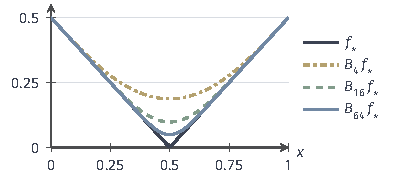
\includegraphics[width=66.7mm]{figures/02-abstract-mathematics/03-function-spaces/tikz/c6-bernstein-approx/figure.pdf}
  \caption{折线$f_*(x)=\lvert x-1/2\rvert$（黑）及其Bernstein多项式$B_4f_*$、$B_{16}f_*$、$B_{64}f_*$。每条曲线都是结点值的凸组合，位于$f_*$上方；一致误差都在$x=1/2$处取得，依次为$0.1875$、$0.0982$、$0.0497$，次数每增至四倍，误差约减半。}
  \label{fig:fapprox-bernstein}
\end{figure}

\paragraph{附加光滑性与误差速率}
定理保证$f_*$能被多项式任意逼近，但任何多项式都不等于$f_*$，因为多项式处处可微。“能任意逼近”与“给定次数下误差多大”是两个问题，后者需要对目标另加定量条件。若$f$是$L$-Lipschitz的，不必作近远分解，直接用Cauchy--Schwarz不等式与式~\eqref{eq:fapprox-bernstein-variance}：
\[
  \lvert B_mf(x)-f(x)\rvert\leq L\sum_j\Bigl\lvert\frac jm-x\Bigr\rvert w_{m,j}(x)\leq L\Bigl(\sum_j\Bigl(\frac jm-x\Bigr)^2w_{m,j}(x)\Bigr)^{1/2}\leq\frac L{2\sqrt m}.
\]
对$f_*$，$L=1$，界在$m=4,16,64$时为$0.25$、$0.125$、$0.0625$，与图~\ref{fig:fapprox-bernstein}中的实际误差同阶。对$\sqrt x$只有$\lvert f(s)-f(t)\rvert\leq\lvert s-t\rvert^{1/2}$，同样的论证（先对$\lvert j/m-x\rvert^{1/2}$用Cauchy--Schwarz）只给出$(4m)^{-1/4}$。条件越弱，这一构造能保证的速率越慢。

更多的光滑性并不能让Bernstein多项式更快。由引理~\ref{lem:fapprox-bernstein-moments}，$B_m(x^2)=x^2+x(1-x)/m$，误差恰为$1/(4m)$量级，而$x^2$本身就是二次多项式，$m\geq2$时最佳误差为零。所以Bernstein构造给出的是对所有连续函数都可验证的收敛机制，不是给定次数下的最佳近似。对最佳多项式逼近误差$E_m(f)=E(f,\mathcal P_m)_\infty$，其中$\mathcal P_m$是次数至多$m$的多项式空间，Jackson型定理给出：若$f\in C^r[a,b]$，则$E_m(f)\leq C_rm^{-r}\omega_{f^{(r)}}(1/m)$，常数$C_r$只依赖$r$与区间。光滑性越高，最佳多项式误差下降越快；对只有折点的$f_*$，最佳误差按$1/m$下降，也不能更快。这两条结论这里都不给出证明。

多项式还有一个结构上的特点：它是全局的。改变一个系数，整个区间上的函数值都会改变；Bernstein权重也在整个$(0,1)$上非零。目标若只在一处不光滑，例如$f_*$的折点，这一处的困难会影响全区间上的近似。下一小节的分段表示把这种影响限制在局部。

\subsection{固定网格上的分段逼近}
\label{sec:fapprox-fixed-grid}

另一种思路是先把区间切成小段，每段只用低次多项式。固定结点$0=t_0<t_1<\cdots<t_N=1$，记网格尺寸$h=\max_i(t_{i+1}-t_i)$。网格在看到目标之前就已经选定，所以候选集合仍是固定的线性空间；预算由单元数$N$和每个单元内的次数共同决定。

\paragraph{分段常数与分段多项式}
最简单的选择是每个单元上取常数。若在单元$[t_i,t_{i+1}]$上取该单元内函数值的最佳常数$(\max+\min)/2$，由第~\ref{sec:fapprox-fixed-space}节，单元上的误差为振幅的一半，因此整体一致误差不超过$\omega_f(h)/2$。若$f\in C^1$，振幅不超过$h\lVert f'\rVert_\infty$，误差至多$h\lVert f'\rVert_\infty/2$，按一阶下降。

每个单元上用$r$次多项式、单元之间不加任何衔接条件时，空间维数为$N(r+1)$。若$f\in C^{r+1}[0,1]$，在每个单元上取$f$在中点$c_i$处的$r$次Taylor多项式，由Taylor余项，单元内
\[
  \lvert f(x)-p_i(x)\rvert\leq\frac{\lVert f^{(r+1)}\rVert_\infty}{(r+1)!}\Bigl(\frac h2\Bigr)^{r+1}.
\]
误差按$h^{r+1}$下降。这是一个可验证的构造，不必是该空间中的最佳近似；它说明提高单元内次数换来的是更高的阶，前提是目标有相应阶的有界导数。

\paragraph{分段线性插值}
在实际中更常用的是连续的分段线性函数。对$x\in[t_i,t_{i+1}]$，令
\begin{equation}
  S_hf(x)=(1-s)f(t_i)+s\,f(t_{i+1}),\qquad s=\frac{x-t_i}{t_{i+1}-t_i}\in[0,1].
  \label{eq:fapprox-linear-interpolant}
\end{equation}
相邻两段在公共结点取同一个值，所以$S_hf$是经过全部结点值的连续折线，称为$f$的\term{分段线性插值}（piecewise linear interpolation）。在每段上为一次函数的全体连续函数组成$N+1$维空间。对每个结点$t_i$，令$\varphi_i$为在$t_i$处取$1$、在其余结点取$0$的连续折线，它在$[t_{i-1},t_{i+1}]$上呈三角形，称为\term{帽形函数}（hat function）。于是$S_hf=\sum_if(t_i)\varphi_i$，系数就是结点值。

\begin{theorem}[分段线性插值的误差]
\label{thm:fapprox-linear-interpolation}
若$f\in C[0,1]$，则$\lVert f-S_hf\rVert_\infty\leq\omega_f(h)$。若进一步$f\in C^2[0,1]$，则
\begin{equation}
  \lVert f-S_hf\rVert_\infty\leq\frac{h^2}8\lVert f''\rVert_\infty .
  \label{eq:fapprox-interpolation-quadratic}
\end{equation}
\end{theorem}

\begin{proof}
在单元$[t_i,t_{i+1}]$上，$f(x)-S_hf(x)=(1-s)\bigl(f(x)-f(t_i)\bigr)+s\bigl(f(x)-f(t_{i+1})\bigr)$。$x$到两端点的距离都不超过$h$，两个差值都不超过$\omega_f(h)$，凸组合也不超过$\omega_f(h)$。

再证二阶界。固定单元内一点$x\in(t_i,t_{i+1})$，令$g=f-S_hf$，它在两端为零。取
\[
  \kappa=\frac{g(x)}{(x-t_i)(x-t_{i+1})},\qquad G(u)=g(u)-\kappa(u-t_i)(u-t_{i+1}),
\]
则$G$在$t_i,x,t_{i+1}$三点为零。两次使用Rolle定理，存在$\xi$使$G''(\xi)=0$。$S_hf$在单元内是一次函数，$G''(\xi)=f''(\xi)-2\kappa$，故
\[
  f(x)-S_hf(x)=\frac{f''(\xi)}2(x-t_i)(x-t_{i+1}).
\]
单元上$\lvert(x-t_i)(x-t_{i+1})\rvert\leq(t_{i+1}-t_i)^2/4\leq h^2/4$，代入即得。
\end{proof}

两个界依据不同。连续模界只用了凸组合，对任何连续目标都成立，也不要求等距：只要网格尺寸$h\to0$，插值就一致收敛。二阶界多用了$f''$的有界性，换来$h^2$的速率。常数$1/8$不能改进：取$f(x)=x^2$与两个结点$0,1$，误差$x-x^2$在$1/2$处取到$1/4=h^2\lVert f''\rVert_\infty/8$。

\paragraph{局部正则性与网格位置}
二阶速率所需的光滑性不能省略。取等距结点$t_i=i/N$，$N$为奇数，此时$1/2$不是结点，而是某个单元的中点。$f_*$在这个单元两端的值都是$h/2$，插值在单元内恒为$h/2$，而$f_*(1/2)=0$；其余单元上$f_*$本身是直线，插值没有误差。所以$\lVert f_*-S_hf_*\rVert_\infty=h/2$，只按一阶下降。图~\ref{fig:fapprox-spline-rates}在对数坐标中比较了光滑目标$\sin(\pi x)$与$f_*$：前者的误差贴近二阶界，后者恰为$h/2$。

\begin{figure}[!htb]
  \centering
  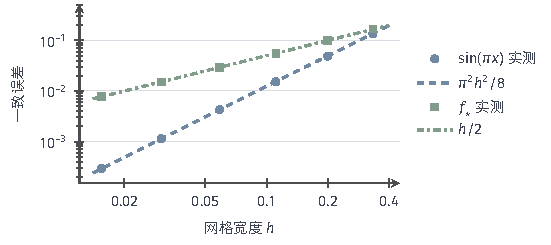
\includegraphics[width=93.4mm]{figures/02-abstract-mathematics/03-function-spaces/tikz/c6-spline-rates/figure.pdf}
  \caption{等距线性插值的一致误差与网格宽度$h=1/N$（$N=3,5,\ldots,65$为奇数，$1/2$不是结点），双对数坐标。光滑目标$\sin(\pi x)$的误差（圆点）贴近二阶界$\pi^2h^2/8$；折线$f_*$的误差（方块）恰为$h/2$，只按一阶下降。}
  \label{fig:fapprox-spline-rates}
\end{figure}

反过来，若结点恰好包含$1/2$，$f_*$在每个单元上都是直线，插值没有误差；用$t_0=0,t_1=1/2,t_2=1$三个结点就有$f_*=\frac12\varphi_0+0\cdot\varphi_1+\frac12\varphi_2$。同一个固定网格空间，对有的目标很有效，对稍微挪动了折点位置的目标就只剩一阶速率。固定网格的误差由目标在每个单元内的局部正则性决定，而折点落在哪个单元，在选网格时并不知道。这正是第~\ref{sec:fapprox-adaptive}节让分点随目标移动的动机。

\paragraph{拼接条件与维数}
单元之间的衔接条件改变维数，但不改变上面的阶。$N$个单元上不衔接的分段线性函数有$2N$维，要求连续后减少$N-1$个自由度，剩下$N+1$维，误差阶仍为$h^2$。更一般地，每段为$k$次多项式、在内部结点处$k-1$阶导数连续的函数称为$k$次\term{样条}（spline）。$N$段各有$k+1$个系数，$N-1$个内部结点各施加$k$个条件，维数为$(k+1)N-k(N-1)=N+k$；常用的三次样条维数为$N+3$。衔接条件让近似更光滑，并以较少的参数达到同样的阶，代价是系数与结点值不再一一对应，插值需要解一个线性方程组。

\paragraph{与全局多项式的比较}
在相同维数下比较两类空间。对光滑目标，维数为$N+1$的分段线性插值误差按$N^{-2}$下降，而次数为$N$的最佳多项式误差按Jackson型估计可以下降得更快；对$f_*$这类只在一点不光滑的目标，两者都只有一阶速率，但分段插值的误差只集中在含折点的一个单元里，其余单元上没有误差。全局多项式利用整体光滑性，分段多项式利用局部光滑性。选择哪一种，取决于目标的光滑性是整体的还是局部的。

\subsection{张量积表示}
\label{sec:fapprox-tensor}

目标有多个变量时，最自然的固定子空间是由一维表示相乘得到的。给定$x$方向的函数$\varphi_1,\ldots,\varphi_m$与$y$方向的函数$\psi_1,\ldots,\psi_n$，乘积$(\varphi_i\otimes\psi_k)(x,y)=\varphi_i(x)\psi_k(y)$称为两者的\term{张量积}（tensor product）。全体乘积的线性组合组成$mn$维空间（每组函数线性无关时），系数排成$m\times n$矩阵；有限维的张量积与Kronecker积可参考\BookChapterRef{chap:linear-operations}{卷二第1章“向量、矩阵与张量的运算”}。

\paragraph{网格插值与组合误差}
在$[0,1]$上取等距结点$t_i=i/(m-1)$，$i=0,\ldots,m-1$，帽形函数为$\varphi_0,\ldots,\varphi_{m-1}$，网格宽度$h=1/(m-1)$。二维插值取
\[
  (\Pi f)(x,y)=\sum_{i=0}^{m-1}\sum_{k=0}^{m-1}f(t_i,t_k)\,\varphi_i(x)\varphi_k(y).
\]
乘积$\varphi_i\otimes\varphi_k$支撑在一个矩形上，任一点只受它所在网格单元四个角点的影响，这就是双线性插值。图~\ref{fig:fapprox-tensor-grid}(a)画出$m=5$时一个乘积基的支撑与一个查询点所用的四个角点。

误差可以由一维结果逐个方向得到，但要多用一条性质。记$I_x$为固定$y$只对$x$作线性插值，$I_y$类似，则$\Pi=I_xI_y$。$I_x$是结点值的凸组合，所以$\lVert I_xg\rVert_\infty\leq\lVert g\rVert_\infty$。若$f\in C^2([0,1]^2)$，由定理~\ref{thm:fapprox-linear-interpolation}，
\[
  \lVert f-\Pi f\rVert_\infty\leq\lVert f-I_xf\rVert_\infty+\lVert I_x(f-I_yf)\rVert_\infty\leq\frac{h^2}8\bigl(\lVert\partial_x^2f\rVert_\infty+\lVert\partial_y^2f\rVert_\infty\bigr).
\]
第二项能用一维误差控制，靠的是$I_x$不放大一致范数；若某个方向的插值算子范数大于$1$，组合后的整体误差会被这个范数放大，单变量误差就不足以控制它。同样的论证在$d$维给出误差至多$d\,h^2\max_i\lVert\partial_i^2f\rVert_\infty/8$。

\paragraph{成本随维数的增长}
误差只随维数线性增大，所需系数个数却是$m^d$。设每个$\lVert\partial_i^2f\rVert_\infty\leq1$，要求误差不超过$\varepsilon=10^{-3}$，上式要求$h^2\leq8\varepsilon/d$。$d=2$时$h\leq0.0632$，取$m=17$，共$289$个系数；$d=6$时$h\leq0.0365$，需要$m=29$，共$29^6\approx5.9\times10^8$个系数。每个方向的分辨率只略有提高，总数却增长了六个数量级。这种由完整组合造成的规模增长称为\term{维数灾难}（curse of dimensionality）。第~\ref{sec:fapprox-fourier-truncation}节的多变量Fourier截断有同样的现象：保留$\max_i\lvert k_i\rvert\leq K$需要$(2K+1)^d$个系数。

\begin{figure}[!htb]
  \centering
  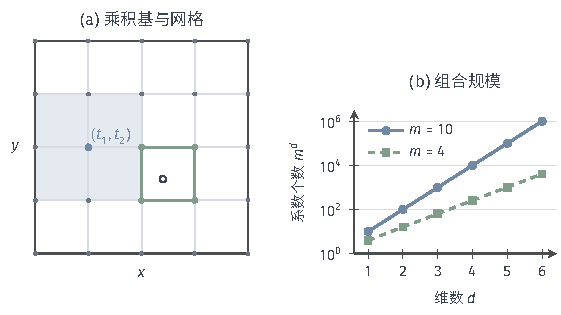
\includegraphics[width=95.0mm]{figures/02-abstract-mathematics/03-function-spaces/tikz/c6-tensor-grid/figure.pdf}
  \caption{张量积网格。(a)每轴$m=5$个结点，蓝底为乘积帽形基$\varphi_1(x)\varphi_2(y)$的支撑，蓝点为其中心结点$(t_1,t_2)$；空心圆为一个查询点，双线性插值只用它所在单元的四个角点（绿）。(b)完整张量积系数个数$m^d$随维数$d$指数增长（对数纵轴）。}
  \label{fig:fapprox-tensor-grid}
\end{figure}

比较成本时要写明计数的对象。上面数的是需要存储的系数，也就是网格上的函数值个数$m^d$；在一个点上求值只用所在单元的$2^d$个角点，代价随维数增长得慢得多；而确定这些系数需要的函数取样次数又与系数个数相同。“维数灾难”指的是前一种计数在固定误差要求下的指数增长，它来自对每个方向都使用同样分辨率的完整组合，并不说明所有多变量逼近都必须付出这样的代价。

\section{最佳N项逼近}
\label{sec:fapprox-best-n-term}

固定子空间对所有目标一视同仁：截断Fourier级数总是保留低频，固定网格总是在同样的位置细分。目标的重要信息若集中在少数几个预先没有选中的方向上，固定选法就会浪费预算。本节仍固定一组完备标准正交基，但允许根据目标挑选保留哪些基向量，只限制挑选的个数。

先用一个向量看这件事。在$\mathbb R^5$中取
\[
 v=(0.1,\ 3,\ -0.2,\ 2,\ 0.4).
\]
若只能留两个坐标，总是留前两个的话，被舍弃的是$-0.2,2,0.4$，平方误差是$0.04+4+0.16=4.2$。若留绝对值最大的两个，即$3$和$2$，被舍弃的是$0.1,-0.2,0.4$，平方误差只有$0.21$。同样的预算，差了二十倍。

设$H$是可分Hilbert空间，$(e_n)_{n\geq1}$是一组标准正交基，$f$的系数为$c_n=\langle e_n,f\rangle$。对预算$N$，令
\[
 \Sigma_N=\Bigl\{\sum_{n\in\Lambda}a_ne_n:\ \Lambda\subseteq\mathbb N,\ \lvert\Lambda\rvert\leq N,\ a_n\in\mathbb K\Bigr\}.
\]

\begin{definition}[最佳N项逼近]
\label{def:fapprox-best-n-term}
称
\begin{equation}
 \sigma_N(f)_2=E(f,\Sigma_N)_H=\inf_{g\in\Sigma_N}\lVert f-g\rVert
 \label{eq:fapprox-best-n-term}
\end{equation}
为$f$关于基$(e_n)$的最佳$N$项误差；达到这个下确界的元素称为$f$的\term{最佳N项逼近}（best N-term approximation）。
\end{definition}

$\Sigma_N$是第~\ref{sec:fapprox-budget}节所说的非线性候选集合。它是所有至多$N$维坐标子空间的并，两个元素之和可能用到$2N$个基向量；图~\ref{fig:fapprox-nearest-point}(c)画的正是$\mathbb R^2$中的$\Sigma_1$。非线性只来自支撑集合$\Lambda$依赖于目标，一旦$\Lambda$选定，近似就是在线性子空间$\operatorname{span}\{e_n:n\in\Lambda\}$中作正交投影。

\subsection{固定截断与自适应选择}
\label{sec:fapprox-fixed-vs-adaptive}

在同一组基和同一个项数下比较两种做法。固定截断预先规定下标集合$\Lambda_N=\{1,\ldots,N\}$，对所有目标都保留前$N$项，误差为
\[
 \Bigl(\sum_{n>N}\lvert c_n\rvert^2\Bigr)^{1/2},
\]
这是第~\ref{sec:fapprox-fixed-space}节在$V_N=\operatorname{span}\{e_1,\ldots,e_N\}$中的最佳逼近。自适应选择则对每个目标分别挑选$\Lambda$。由定义，$\sigma_N(f)_2$不超过固定截断的误差，差距取决于大系数是否恰好排在前面。

极端情形下差距可以达到最大。取$f=e_{N+1}$，固定截断的误差为$\lVert f\rVert=1$，而一项就能精确表示它，$\sigma_1(f)_2=0$。不那么极端的情形同样常见：一个大部分区域光滑、只在某处有跳跃的函数，在小波基中的大系数集中在跳跃附近的细尺度上，按“先粗后细、从左到右”的固定次序要保留许多无用的系数才能轮到它们。

自适应选择的代价是需要知道系数的大小。要挑出重要的系数，通常得先计算或估计足够多的系数，再按大小筛选；被挑出的下标集合也要存储，它本身就是表示的一部分。所以最佳$N$项误差衡量的是“已知全部系数时用$N$项能做到多好”，它与在有限计算下找到这些项的问题是两回事。

\subsection{最大系数选择}
\label{sec:fapprox-largest-coefficients}

在正交基和$L^2$型范数下，最佳$N$项逼近有简单的显式解。由$f\in H$，$\sum_n\lvert c_n\rvert^2<\infty$，所以对任意$t>0$，满足$\lvert c_n\rvert\geq t$的下标只有有限个。于是可以把系数的绝对值按非增次序排列为
\[
 c_1^*\geq c_2^*\geq\cdots
\]
相等的值任意排序，非零系数有限时在末尾补零。

\begin{theorem}[保留最大系数最优]
\label{thm:fapprox-largest-coefficients}
设$\Lambda_N^*$是$\lvert c_n\rvert$最大的$N$个下标组成的集合，$g_N=\sum_{n\in\Lambda_N^*}c_ne_n$。则$g_N$是$f$的最佳$N$项逼近，并且
\begin{equation}
 \sigma_N(f)_2^2=\sum_{n>N}(c_n^*)^2 .
 \label{eq:fapprox-largest-coefficients}
\end{equation}
\end{theorem}

\begin{proof}
任取$\lvert\Lambda\rvert\leq N$与系数$a_n$，令$g=\sum_{n\in\Lambda}a_ne_n$。由Parseval等式，$f-g$的平方范数按坐标拆开：
\[
 \lVert f-g\rVert^2=\sum_{n\in\Lambda}\lvert c_n-a_n\rvert^2+\sum_{n\notin\Lambda}\lvert c_n\rvert^2 .
\]
第一项非负，在$a_n=c_n$时为零。所以对固定的$\Lambda$，最好的系数就是原系数，于是
\[
 \lVert f-g\rVert^2\geq\sum_{n\notin\Lambda}\lvert c_n\rvert^2=\lVert f\rVert^2-\sum_{n\in\Lambda}\lvert c_n\rvert^2 .
\]

$\Lambda$至多含$N$个下标，$\sum_{n\in\Lambda}\lvert c_n\rvert^2$不超过最大的$N$个平方之和，等号在$\Lambda=\Lambda_N^*$时取到。所以
\[
 \lVert f-g\rVert^2\geq\lVert f\rVert^2-\sum_{n\leq N}(c_n^*)^2=\sum_{n>N}(c_n^*)^2 ,
\]
而$g_N$达到这个下界。
\end{proof}

证明依赖两件事。第一，误差平方能拆成各方向上的平方和，这来自基的正交性和Parseval等式。第二，这种拆分让“选哪些方向”与“选什么系数”分开处理。若基不正交，或使用冗余的字典，同一个函数有多种展开，系数本身不唯一，误差也不再是舍弃系数的平方和。

换一把尺子同样会出问题。用下面的Haar基，取$f=1.2\varphi+\psi_{2,0}$，一致范数下比较保留哪一项。$\psi_{2,0}$在$[0,\frac18)$上取$2$、在$[\frac18,\frac14)$上取$-2$，其余为零。按最大系数规则保留系数$1.2$的$\varphi$，则对任何$a$，$f-a\varphi$在这两段上相差$4$，所以
\[
 \lVert f-a\varphi\rVert_\infty\geq2 .
\]
改为保留系数较小的$\psi_{2,0}$，误差只有$\lVert1.2\varphi\rVert_\infty=1.2$。原因是细尺度的基函数高而窄，系数小但一致范数大。

\paragraph{Haar展开中的选择}
用第~\ref{chap:wavelet-transform}章的Haar基复算这一选择。在$L^2(0,1)$上，记
\[
 \varphi=\mathbf 1_{[0,1)},\qquad \psi=\mathbf 1_{[0,1/2)}-\mathbf 1_{[1/2,1)},\qquad \psi_{j,k}(x)=2^{j/2}\psi(2^jx-k),
\]
其中$j\geq0$，$0\leq k<2^j$；$\varphi$与全体$\psi_{j,k}$组成标准正交基。取在$3/4$处向下跳跃的阶梯函数
\[
 f=3\cdot\mathbf 1_{[0,3/4)}-\mathbf 1_{[3/4,1)} .
\]

逐个计算内积。$\varphi$的系数就是平均值：
\[
 \langle\varphi,f\rangle=\frac{3\cdot3-1}4=2 .
\]
$\psi_{0,0}$的系数是左半积分减右半积分：
\[
 \langle\psi_{0,0},f\rangle=\int_0^{1/2}f-\int_{1/2}^1f=\frac32-\frac12=1 .
\]
下一层的两个系数分别是
\[
 \langle\psi_{1,0},f\rangle=0,\qquad
 \langle\psi_{1,1},f\rangle=\sqrt2\Bigl(\int_{1/2}^{3/4}f-\int_{3/4}^1f\Bigr)=\sqrt2 .
\]
$j\geq2$时，$\psi_{j,k}$支撑在某个长为$1/4$的二进区间内且积分为零，$f$在这样的区间上是常数，内积为零。

于是$f$只有三个非零坐标：
\[
 f=2\varphi+\psi_{0,0}+\sqrt2\,\psi_{1,1}.
\]
用Parseval等式检验：$\lVert f\rVert^2=(9\cdot3+1)/4=7$，而$2^2+1^2+(\sqrt2)^2=7$。

按“先粗后细、同层从左到右”的固定次序$\varphi,\psi_{0,0},\psi_{1,0},\psi_{1,1},\ldots$截断，保留两项得$2\varphi+\psi_{0,0}$，误差平方为$2$；保留三项仍缺$\psi_{1,1}$，误差平方仍为$2$。系数绝对值的非增排列是$2,\sqrt2,1,0,\ldots$，由定理~\ref{thm:fapprox-largest-coefficients}，最佳两项逼近为$2\varphi+\sqrt2\,\psi_{1,1}$，误差平方为
\[
 \sigma_2(f)_2^2=1 .
\]
最佳三项逼近就是$f$本身，$\sigma_3(f)_2=0$。

图~\ref{fig:fapprox-best-n-term}对照了两种选择。固定次序的近似在跳跃所在的右半区间上偏差最大；最佳两项逼近把预算用到了$\psi_{1,1}$，正好捕捉到跳跃，代价是在左半区间留下幅度为$1$的偏差。跳跃位于右半区间的细尺度上，固定次序先用掉了左半区间那个为零的系数，自适应选择直接找到了它。

\begin{BookInlineFigure}
  \centering
  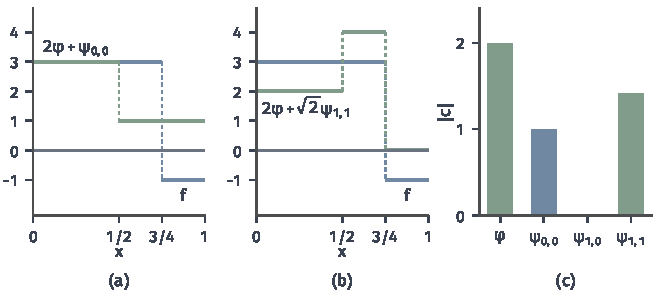
\includegraphics[width=112mm]{figures/04-spaces-measures-and-geometry/03-function-spaces/matplotlib/fapprox-best-n-term/figure.pdf}
  \caption{同一预算下的两种选择。目标$f$（蓝）在$3/4$处跳跃，均保留两项（绿）。(a)固定次序保留$\varphi,\psi_{0,0}$，误差平方为$2$。(b)保留系数最大的$\varphi,\psi_{1,1}$，误差平方为$1$。(c)前四个Haar系数的绝对值，绿色为最佳两项选中的系数；固定次序选的是前两根柱子。}
  \label{fig:fapprox-best-n-term}
\end{BookInlineFigure}

\section{自适应分段逼近}
\label{sec:fapprox-adaptive}

第~\ref{sec:fapprox-fixed-grid}节的固定网格在看到目标之前就选定了分点，误差由目标在最差单元上的局部正则性决定。若目标只在少数地方变化剧烈，更合理的做法是在那里多放分点，在平缓处少放。上一节只调整“留哪几个坐标”，这里连坐标轴本身也按目标调整：分点就是把长向量的下标切成几段的位置。

本节把预算固定为区间个数$N$，允许分点随目标移动，在一致范数下比较固定网格与自适应分割，并区分三个问题：最佳分割是否存在，它的误差有多大，以及怎样找到一个好的分割。

\paragraph{候选集合与局部误差}
在$[0,1]$上，令$\mathcal S_N$为全体至多$N$段的分段常数函数：存在$0=x_0\leq x_1\leq\cdots\leq x_N=1$，函数在每个$[x_{i-1},x_i)$上为常数，最后一段含右端点。分点是候选的一部分，所以$\mathcal S_N$不是线性空间，相应的逼近称为\term{自适应分段逼近}（adaptive piecewise approximation）。

分割固定后，每段上的最佳常数由式~\eqref{eq:fapprox-best-constant}给出：在$I=[a,b]$上，局部误差是振幅的一半，记为$\frac12\operatorname{osc}(f,I)$，其中$\operatorname{osc}(f,I)=\max_If-\min_If$。所以对连续的$f$，
\begin{equation}
 E(f,\mathcal S_N)_\infty=\frac12\inf_{0=x_0\leq\cdots\leq x_N=1}\ \max_{1\leq i\leq N}\operatorname{osc}\bigl(f,[x_{i-1},x_i]\bigr).
 \label{eq:fapprox-adaptive-error}
\end{equation}
寻找最佳逼近化成了一个只关于分点的问题：让最大的局部振幅尽可能小。

\paragraph{平方根函数的比较}
以$f(x)=\sqrt x$为例。它在$[0,1]$上连续递增，但在原点附近导数无界，不是Lipschitz的。等距网格$x_i=i/N$上，单元$[x_{i-1},x_i]$的振幅是
\[
 \sqrt{\frac iN}-\sqrt{\frac{i-1}N},
\]
随$i$递减，最大的是第一个单元的$\sqrt{1/N}$。所以固定网格的误差为
\[
 \frac1{2\sqrt N}.
\]

若改取$x_i=(i/N)^2$，每个单元的振幅都是
\[
 \sqrt{x_i}-\sqrt{x_{i-1}}=\frac1N ,
\]
误差为$1/(2N)$。$N=100$时，前者为$0.05$，后者为$0.005$。分点向原点聚集，把局部误差平均分配到各个单元。图~\ref{fig:fapprox-adaptive}(a)(b)画出$N=6$的两种分割。

这个分割还是最优的。任一分割的各段振幅之和为
\[
 \sum_i\bigl(\sqrt{x_i}-\sqrt{x_{i-1}}\bigr)=1 ,
\]
$N$个数之和为$1$，最大者不小于$1/N$。所以$E(\sqrt{\cdot},\mathcal S_N)_\infty=1/(2N)$，自适应分段把速率从$N^{-1/2}$提高到$N^{-1}$，而固定网格要达到同样的速率需要目标是Lipschitz的。

\begin{BookInlineFigure}
  \centering
  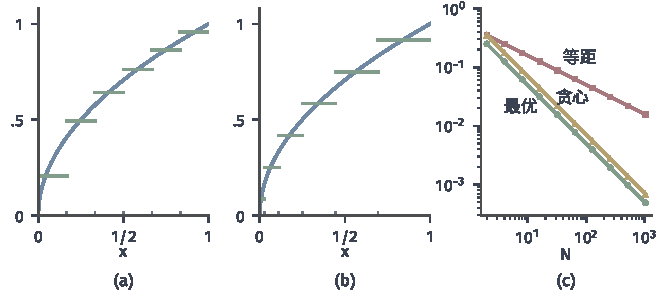
\includegraphics[width=112mm]{figures/04-spaces-measures-and-geometry/03-function-spaces/matplotlib/fapprox-adaptive/figure.pdf}
  \caption{$\sqrt x$的分段常数逼近，每段取最佳常数（绿），下方刻线为分点。(a)$N=6$的等距分割，误差集中在第一段。(b)$N=6$的分割$x_i=(i/6)^2$，每段振幅相同。(c)一致误差随段数$N$的变化，双对数坐标：等距为$1/(2\sqrt N)$，最优为$1/(2N)$，二进贪心细分的误差约为最优的$\sqrt2$倍。}
  \label{fig:fapprox-adaptive}
\end{BookInlineFigure}

\paragraph{单调函数的误差界}
平方根例子中用到的只是单调性，并不需要可微。把振幅之和等于总变化量的论证写成一般形式，就得到下面的结论。

\begin{theorem}[单调函数的自适应分段误差]
\label{thm:fapprox-monotone}
设$f$在$[a,b]$上连续且单调，$V=\lvert f(b)-f(a)\rvert$。则
\begin{equation}
 E(f,\mathcal S_N)_\infty=\frac V{2N},
 \label{eq:fapprox-monotone}
\end{equation}
并且存在达到这一误差的分割。
\end{theorem}

\begin{proof}
不妨设$f$不减。对任一分割，各段振幅为$f(x_i)-f(x_{i-1})$，其和为$V$，最大者不小于$V/N$，所以误差不小于$V/(2N)$。

反过来，令$x_0=a$，对$i=1,\ldots,N$取
\[
 x_i=\min\Bigl\{x\in[a,b]:\ f(x)=f(a)+\frac{iV}N\Bigr\}.
\]
由介值定理这样的点存在，由连续性最小值能取到，水平递增时这些点不减。$x_N\leq b$，把最后一个分点改成$b$，$f$在多出的一段上恒为$f(b)$，不改变取值范围。

在$[x_{i-1},x_i]$上，$f$的取值落在$f(a)+(i-1)V/N$与$f(a)+iV/N$之间，振幅不超过$V/N$。由式~\eqref{eq:fapprox-adaptive-error}，误差不超过$V/(2N)$。
\end{proof}

定理把误差与总变化量$V$联系起来，而不是与导数或连续模联系。固定网格的误差由$\omega_f(h)$控制，要求处处都不能变化太快；自适应分割只要求变化的总量有限，变化集中在哪里都可以。在同一预算和同一误差范数下，两种候选集合对目标正则性的要求不同。

\paragraph{最佳分割的存在}
对一般的连续函数，最佳分割同样存在，但通常没有显式公式。分点向量$(x_1,\ldots,x_{N-1})$在紧集$\{0\leq x_1\leq\cdots\leq x_{N-1}\leq1\}$中变化。由$f$一致连续，$\operatorname{osc}(f,[a,b])$是$(a,b)$的连续函数：端点移动不超过$\eta$时，最大值与最小值各自至多改变$\omega_f(\eta)$。

所以最大局部振幅是分点的连续函数，在紧集上取到最小值。允许相邻分点重合，相当于允许少于$N$段，并不改变$\mathcal S_N$。这一论证和第~\ref{sec:fapprox-fixed-space}节的存在定理一样靠紧性，只是紧的集合从有限维子空间中的闭球换成了分点的单纯形。

存在性与误差界是两回事。存在性论证没有说明最佳误差有多大，也没有给出找到最佳分割的方法；单调函数的定理给出了误差的精确值，构造却依赖于知道$f$的水平集位置。

\paragraph{贪心细分}
实际中常用的是一种简单的算法：从整个区间出发，每一步找出局部误差最大的单元，把它从中点一分为二，直到用完$N$个单元。每步只需计算新产生的两个单元的振幅，分点都落在二进点上。

用$\sqrt x$跑前几步。第一步把$[0,1]$对半切，两段的振幅是
\[
 \operatorname{osc}\bigl(\sqrt{\cdot},[0,\tfrac12]\bigr)=0.7071,\qquad
 \operatorname{osc}\bigl(\sqrt{\cdot},[\tfrac12,1]\bigr)=0.2929 .
\]
第二步切振幅最大的$[0,\frac12]$，得到$[0,\frac14]$的振幅$0.5$和$[\frac14,\frac12]$的振幅$0.2071$。第三步切$[0,\frac14]$，得到振幅$0.3536$和$0.1464$。

这时四个单元从左到右的振幅是
\[
 0.3536,\quad 0.1464,\quad 0.2071,\quad 0.2929 .
\]
最大误差是$0.3536/2=0.1768$，而$N=4$的最优误差是$1/8=0.125$。贪心细分总是先切靠近原点的单元，却只能对半切，各单元的振幅不能像最优分割那样恰好相等。

表~\ref{tab:fapprox-greedy}列出了几种$N$的结果。这个例子中贪心误差始终是最优误差的约$\sqrt2$倍，也就是说，它达到了与最优分割相同的速率$N^{-1}$，只损失一个常数。这是对$\sqrt x$的计算观察，不是一般定理；贪心细分与最佳误差的比较需要针对目标类另作分析。

\begin{BookInlineTable}
  \centering
  \caption{$\sqrt x$的分段常数逼近的一致误差}
  \label{tab:fapprox-greedy}
  \begin{tabular}{rlll}
    \toprule
    $N$ & 等距$1/(2\sqrt N)$ & 贪心细分 & 最优$1/(2N)$ \\
    \midrule
    $4$ & $0.25$ & $0.1768$ & $0.125$ \\
    $16$ & $0.125$ & $0.0442$ & $0.0313$ \\
    $64$ & $0.0625$ & $0.0110$ & $0.0078$ \\
    $1024$ & $0.0156$ & $0.00069$ & $0.00049$ \\
    \bottomrule
  \end{tabular}
\end{BookInlineTable}

二进的贪心细分与上一节的Haar展开密切相关：在二进区间上保留或舍去细分，相当于在Haar展开中保留或舍去对应的细节系数。哪些函数能被这样的自适应表示以给定速率逼近，可以用函数在不同尺度上的局部变化来刻画，这正是第~\ref{chap:besov-spaces}章研究的问题。

\section{本章小结}
\label{sec:fapprox-summary}

本章开头问：哪些简单函数能以任意精度逼近目标，加入表示预算后最佳误差又怎样随预算变化。对第一个问题，答案依赖测度、积分指数与误差范数。在任意测度空间中，截断与二进分层的简单函数在$L^p$（$1\leq p<\infty$）中稠密；在Lebesgue区域上，有理矩形与有理复系数给出可数稠密族，$L^p$可分，一般测度空间则要另核集合族条件。欧氏开集上，开紧逼近给出紧支撑连续函数的逼近，平移在$L^p$中连续，磨光误差由平移误差控制，于是光滑紧支撑函数也稠密，局部结论通过截断得到。这些结论在$L^\infty$中都失效：$L^\infty[0,1]$不可分，连续函数与跳跃函数的距离不小于跳跃的一半，尽管简单函数仍能按本质上确界逼近有界函数。

这些都是定性结论。为了比较效率，第~\ref{sec:fapprox-error}节用到候选集合的距离定义最佳逼近误差，并区分最佳误差与具体构造的误差、单个函数的误差与整类函数的最坏误差；后者在有限候选集合下正是覆盖数的问题。有限维子空间中最佳逼近总存在，Hilbert空间中由正交投影唯一给出，其他范数下可以不唯一，最佳选择的映射也不必是线性的。Fourier截断的平方误差等于被舍弃系数的平方和，一致误差由绝对尾和控制，两者要求的系数衰减不同；离散计算还带来与截断分开记账的混叠误差。连续频带截断给出带限函数中的最佳$L^2$逼近，但带限函数空间是无限维的，有限计算还需进一步离散。

后三节比较了三种候选集合。固定子空间对所有目标相同：多项式由次数控制，Bernstein构造给出连续模控制的收敛，附加光滑性带来更快的最佳速率；固定网格上的分段多项式由网格尺寸和每个单元内的局部正则性控制，拼接条件减少维数而不改变阶；张量积让误差随维数线性增长，系数个数却按$m^d$增长。最佳$N$项逼近固定正交基但按目标挑选支撑，在$L^2$中保留最大的$N$个系数最优，$\sigma_N(f)_2^2=\sum_{n>N}(c_n^*)^2$；结论依赖正交性与Parseval等式，不能直接搬到冗余字典或其他范数。自适应分段让分点随目标移动，对单调函数误差精确等于总变化量除以$2N$，对$\sqrt x$把速率从$N^{-1/2}$提高到$N^{-1}$；最佳分割的存在、误差界与找到分割的算法是三个不同的问题。

本章的误差估计都需要对目标的某种正则性作出假设：连续模、有界导数、系数衰减或总变化量。随后三章分别给出系统的刻画：第~\ref{chap:sobolev-spaces}章用弱导数与积分范数控制光滑性，第~\ref{chap:besov-spaces}章用不同尺度上的局部变化刻画非线性逼近的速率，第~\ref{chap:rkhs}章从离散点值观测出发研究插值与逼近。


\chapter{Sobolev空间}
\label{chap:sobolev-spaces}
\label{chap:weak-derivatives-sobolev}

在区间$(0,1)$上，$\sin(2\pi nx)$的平方积分不随$n$改变，可是$n$越大，函数振荡得越快。只用$L^2$范数衡量大小，就看不出这种差别。反过来，若要求函数有连续导数，又会把$|x-1/2|$这样只有一个折点、其余处处光滑的函数排除在外。我们需要一种既能感知变化快慢、又允许适度不光滑的度量方式：同时控制函数本身和它的弱导数。

第~\ref{chap:smoothing-weak-derivatives}章已经用测试函数的积分恒等式定义了弱导数，并证明了磨光与弱导数可以交换。本章先用振荡、折点与跳跃三类例子说明为什么要把弱导数纳入范数，然后建立Sobolev范数，证明空间完备，并在平方可积时得到Hilbert结构。完备性回答了“极限是否留在空间中”，接下来的三节研究空间中能做哪些操作：光滑函数是否稠密，函数能否越过边界延拓到更大的区域，边界条件和零均值条件怎样表述为子空间，并使导数单独给出等价范数。

最后两节研究Sobolev范数能控制什么。连续嵌入回答单个函数的可积性能提高到哪个指数、何时具有连续代表；紧嵌入回答有界函数列能否在较弱的范数下选出强收敛子列，以及有界函数类能否被有限个代表覆盖。这两类结论在临界指数处出现实质差别，我们将用具体的集中序列说明。

本章只处理整数阶空间，重点在一阶空间$W^{1,p}$。弱导数的定义、唯一性和一维绝对连续代表都回用第~\ref{chap:smoothing-weak-derivatives}章，不再重复证明。分数阶的光滑性以及按尺度汇总的变化刻画留到第~\ref{chap:besov-spaces}章，具有连续点值读取的Hilbert函数空间留到第~\ref{chap:rkhs}章。本章函数均取实值，复值函数对实部和虚部分别处理即可。

\section{导数控制}
\label{sec:sobolev-derivative-control}

$L^2$范数把函数在整个区间上的平方大小累加起来，它记录“有多大”，不记录“变化有多快”。本节在$(0,1)$上比较四类函数：频率不同的正弦、常数、带一个折点的函数和阶跃函数。正弦说明只看$L^2$会遗漏振荡，常数说明只看导数会遗漏高度，折点和跳跃则要求我们决定，哪些不能经典求导的函数仍应计入。

\subsection{振荡函数}
\label{sec:sobolev-oscillation}

对正整数$n$，取$f_n(x)=\sin(2\pi nx)$，$0<x<1$。先算它的$L^2$大小。由$\sin^2\theta=(1-\cos2\theta)/2$，而$\cos(4\pi nx)$在$(0,1)$上恰好走过$2n$个完整周期，积分为零，所以
\[
\lVert f_n\rVert_2^2=\int_0^1\sin^2(2\pi nx)\,\mathrm dx=\frac12.
\]
于是
\[
\lVert f_n\rVert_2=\frac1{\sqrt2},
\]
这个值与$n$无关。

导数的情形完全不同。经典导数是$f_n'(x)=2\pi n\cos(2\pi nx)$，同样的计算给出
\begin{equation}
\lVert f_n'\rVert_2=2\pi n\cdot\frac1{\sqrt2}=\sqrt2\,\pi n .
\label{eq:sobolev-oscillation-derivative}
\end{equation}
图~\ref{fig:sobolev-oscillation}把两件事放在一起：左边$f_1$与$f_4$的振幅相同、$L^2$长度相同，右边导数的$L^2$范数却随$n$线性增长。导数范数记录的是函数在单位长度内上下摆动的程度。

\begin{BookInlineFigure}
  \centering
  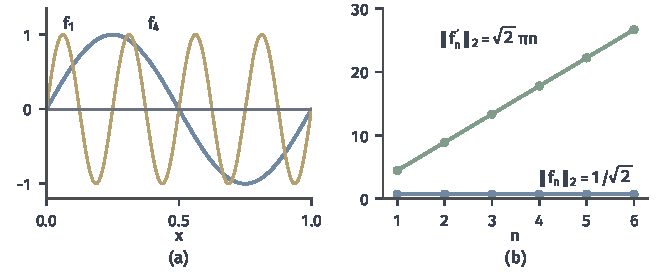
\includegraphics[width=112mm]{figures/04-spaces-measures-and-geometry/03-function-spaces/matplotlib/sobolev-oscillation/figure.pdf}
  \caption{振荡在$L^2$范数中不可见。(a)蓝色为$f_1$，黄色为$f_4$，其中$f_n(x)=\sin(2\pi nx)$，两者的$L^2$长度都是$1/\sqrt2$。(b)蓝点为$\lVert f_n\rVert_2$，保持不变；绿点为$\lVert f_n'\rVert_2$，按式~\eqref{eq:sobolev-oscillation-derivative}随$n$线性增长。}
  \label{fig:sobolev-oscillation}
\end{BookInlineFigure}

\paragraph{高频坐标上的权重}
用向量的语言重述这个现象。把$\sqrt2\sin(2\pi nx)$看成$L^2(0,1)$中的单位向量，它们两两正交，$f_n$就是沿第$n$条坐标轴、长度为$1/\sqrt2$的向量。求导把这条轴送到余弦轴上，同时把长度乘以$2\pi n$。所以频率越高的坐标，求导后放大得越多。

若把长度的平方改成“函数的平方加导数的平方”，第$n$条轴上的贡献就变成
\[
\lVert f_n\rVert_2^2+\lVert f_n'\rVert_2^2
=\frac12\bigl(1+(2\pi n)^2\bigr).
\]
这里的$1+(2\pi n)^2$就是一个权，高频坐标的权大，低频坐标的权小。把导数放进范数，相当于把各向同性的球压扁成沿高频方向很短的椭球。

有限维里可以把这件事完整算出来。取三个等距点上的取值$u=(u_1,u_2,u_3)$，用相邻差分$Du=(u_2-u_1,\ u_3-u_2)$代替导数。差分的平方和是一个二次型：
\[
\lVert Du\rVert^2=u^\top D^\top Du,\qquad
D^\top D=\begin{bmatrix}1&-1&0\\-1&2&-1\\0&-1&1\end{bmatrix}.
\]

这个矩阵的三个特征向量正好是三种“形状”，下面逐个验证。常向量$c=(1,1,1)$的相邻差为零，$D^\top Dc=0$，特征值是$0$。斜坡$t=(1,0,-1)$满足$D^\top Dt=t$，特征值是$1$。锯齿$z=(1,-2,1)$满足
\[
D^\top Dz=(3,-6,3)=3z,
\]
特征值是$3$。形状越“抖”，特征值越大。

于是在这组正交方向上，$\lVert u\rVert^2+\lVert Du\rVert^2$就是把三个坐标分别乘以权$1,2,4$再求和。以$z$为例：
\[
\lVert z\rVert^2=6,\qquad Dz=(-3,3),\qquad \lVert Dz\rVert^2=18=3\lVert z\rVert^2.
\]
函数空间的情形是同一幅图，只是坐标有无穷多个，权也趋于无穷。有限维时权总是有界的；无限维时权无界，这就是求导在$L^2$上不是有界算子的原因。

\paragraph{常数方向}
上面的权里常向量对应的导数项是零，这一点在函数上同样成立。常数函数$c$的导数为零，$\lVert c'\rVert_2=0$对每个$c$成立，只看导数无法区分$c=0$和$c=100$。导数度量变化，函数处在什么高度要由函数本身的大小记录。

所以完整的度量必须同时保留$\lVert f\rVert_2$和$\lVert f'\rVert_2$，也就是上面权里的“$1$”。只有附加零边界或零均值条件、排除了常数方向以后，导数才可能单独控制函数，这是第~\ref{sec:sobolev-derivative-norms}小节的问题。

\subsection{折点与跳跃}
\label{sec:sobolev-kinks-jumps}

若坚持经典导数，$f(x)=|x-1/2|$就会被排除：它只在$x=1/2$处没有导数，其余各点都光滑，变化速度恒为$1$。可是从“累积变化量”的角度看，这个函数没有任何异常。我们用第~\ref{chap:smoothing-weak-derivatives}章的弱导数来检查它。

令$g(x)=\operatorname{sgn}(x-1/2)$，即$x<1/2$时取$-1$，$x>1/2$时取$1$。任取测试函数$\varphi\in C_c^\infty(0,1)$，在折点两侧分别分部积分：
\[
\begin{aligned}
\int_0^1 f\varphi'\,\mathrm dx
&=\int_0^{1/2}\Bigl(\frac12-x\Bigr)\varphi'\,\mathrm dx
+\int_{1/2}^1\Bigl(x-\frac12\Bigr)\varphi'\,\mathrm dx\\
&=\int_0^{1/2}\varphi\,\mathrm dx-\int_{1/2}^1\varphi\,\mathrm dx
=-\int_0^1 g\varphi\,\mathrm dx .
\end{aligned}
\]
边界项在$x=1/2$处都含因子$f(1/2)=0$，在端点处$\varphi$为零，所以全部消失。按弱导数的定义，$f'=g$。

折点函数和它的弱导数都平方可积，大小可以直接算出：
\[
\lVert f\rVert_2^2=2\int_0^{1/2}t^2\,\mathrm dt=\frac1{12},\qquad
\lVert f'\rVert_2^2=1 .
\]
单点不能经典求导并不妨碍用$\lVert f\rVert_2$和$\lVert f'\rVert_2$同时控制它。把这类函数放在一起，就得到第~\ref{sec:sobolev-norms-completeness}节将记为$H^1(0,1)$的空间。

阶跃函数的情形不同。令$H=\mathbf 1_{[1/2,1)}$，对测试函数$\varphi$计算
\begin{equation}
-\int_0^1 H\varphi'\,\mathrm dx=-\int_{1/2}^1\varphi'\,\mathrm dx=\varphi(1/2).
\label{eq:sobolev-step-action}
\end{equation}
跳跃把测试函数送到它在跳跃点的取值，图~\ref{fig:sobolev-kink-step}的(d)画的就是这一作用。

\begin{BookInlineFigure}
  \centering
  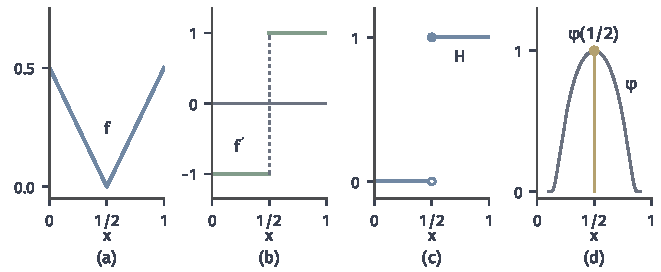
\includegraphics[width=112mm]{figures/04-spaces-measures-and-geometry/03-function-spaces/matplotlib/sobolev-kink-step/figure.pdf}
  \caption{折点与跳跃。(a)折点函数$f(x)=|x-1/2|$，连续。(b)它的弱导数$f'$，在$x=1/2$处跳跃，但仍是平方可积的函数。(c)阶跃函数$H$，在$x=1/2$处跳跃。(d)$H$对测试函数$\varphi$的作用只读取$\varphi(1/2)$，黄色竖线所示；这一作用集中在一点，不是任何函数的积分。}
  \label{fig:sobolev-kink-step}
\end{BookInlineFigure}

这个作用不能写成函数的积分。假设有局部可积函数$h$使$\int_0^1h\varphi\,\mathrm dx=\varphi(1/2)$对所有测试函数成立。对支撑不含$1/2$的$\varphi$，右端是零，由测试函数判别，$h$在$(0,1/2)$和$(1/2,1)$上都几乎处处为零。于是$h=0$几乎处处，而这与取$\varphi(1/2)\neq0$的测试函数矛盾。所以$H$没有弱导数，不属于上述空间。

阶跃函数在$x\neq1/2$处的经典导数是零，所以几乎处处导数是$0$。但$0$并不是它的弱导数，否则$H$几乎处处为常数。这个例子提醒我们，Sobolev空间中的“导数”始终指弱导数，几乎处处存在的经典导数不能自动代替它。

\paragraph{用余弦坐标比较}
现在把这些例子放到同一组坐标里。在$L^2(0,1)$上取正交归一基
\begin{equation}
e_0(x)=1,\qquad e_n(x)=\sqrt2\cos(\pi nx)\quad(n\geq1).
\label{eq:sobolev-cosine-basis}
\end{equation}
它是把函数偶延拓到$(-1,1)$后的Fourier基，完备性来自第~\ref{chap:fourier-transform}章。函数$f$的坐标是$a_n=\int_0^1fe_n\,\mathrm dx$，Parseval等式给出$\lVert f\rVert_2^2=\sum_na_n^2$。选用余弦基的原因在第~\ref{sec:sobolev-hk}小节说明。

先算折点函数的坐标。$f$关于$x=1/2$对称，而$n$为奇数时$\cos(\pi nx)$关于$x=1/2$反对称，所以奇数项为零。取$n=2m$，分部积分得
\[
\int_0^{1/2}\Bigl(\frac12-x\Bigr)\cos(2\pi mx)\,\mathrm dx
=\frac{1-\cos(\pi m)}{(2\pi m)^2}.
\]
因此$a_0=1/4$，而$n=2m$时
\[
a_{2m}=\frac{\sqrt2}{\pi^2m^2}\quad(m\text{为奇数}),\qquad
a_{2m}=0\quad(m\text{为偶数}).
\]

再算阶跃函数的坐标。$a_0=1/2$，$n\geq1$时直接积分得
\[
a_n=\sqrt2\int_{1/2}^1\cos(\pi nx)\,\mathrm dx
=-\frac{\sqrt2\,\sin(\pi n/2)}{\pi n}.
\]
所以偶数项为零，奇数项的绝对值是$\sqrt2/(\pi n)$。折点的坐标按$1/n^2$衰减，阶跃的坐标只按$1/n$衰减。

把坐标乘上权$\pi^2n^2$后求部分和，令$S_N=\sum_{n\leq N}\pi^2n^2a_n^2$。折点函数只有$n=2m$（$m$为奇数）的项，每项是
\[
\pi^2(2m)^2\cdot\frac{2}{\pi^4m^4}=\frac{8}{\pi^2m^2},
\]
再用$\sum_{m\text{奇}}m^{-2}=\pi^2/8$，得到$S_N\to1$，恰好等于$\lVert f'\rVert_2^2$。

阶跃函数的每个奇数项都是
\[
\pi^2n^2\cdot\frac{2}{\pi^2n^2}=2,
\]
所以$S_N$随$N$线性增长，趋于无穷。图~\ref{fig:sobolev-cosine-coordinates}对比了这两条路径：折点函数的加权和收敛到$1$，阶跃函数的加权和发散。

\begin{BookInlineFigure}
  \centering
  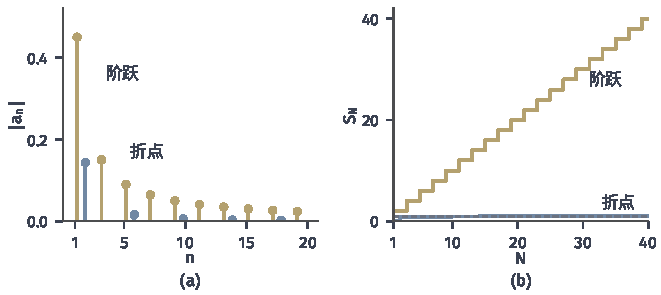
\includegraphics[width=112mm]{figures/04-spaces-measures-and-geometry/03-function-spaces/matplotlib/sobolev-cosine-coordinates/figure.pdf}
  \caption{折点与阶跃的余弦坐标。蓝色为折点函数$|x-1/2|$，黄色为阶跃函数$\mathbf 1_{[1/2,1)}$。(a)坐标的绝对值$|a_n|$，$n\geq1$。(b)加权部分和$S_N=\sum_{n\leq N}\pi^2n^2a_n^2$，虚线高度为$1$，折点的部分和收敛到这一高度，阶跃的部分和线性增长。}
  \label{fig:sobolev-cosine-coordinates}
\end{BookInlineFigure}

这就是用坐标看到的结论：Sobolev范数有限，等于坐标在加权后仍然平方可和。至于阶跃这样的跳跃应当怎样按尺度度量，第~\ref{chap:besov-spaces}章会用平移差回答。

\section{Sobolev范数与完备性}
\label{sec:sobolev-norms-completeness}

上一节的例子要求把函数与它的弱导数放在一起度量。本节固定三项数据，即区域$\Omega$、导数的最高阶数$k$和积分指数$p$，用$L^p$范数分别度量函数及各阶弱导数，再合成一个范数。然后证明这样得到的空间完备，并在$p=2$时写出它的内积和坐标形式。

\subsection{空间的定义}
\label{sec:sobolev-space-definition}

先约定记号。在欧氏开集$\Omega\subset\mathbb R^d$上，多重指标$\alpha=(\alpha_1,\ldots,\alpha_d)$由非负整数组成，$|\alpha|=\alpha_1+\cdots+\alpha_d$是导数的总阶数。$\partial^\alpha f$表示第~\ref{chap:smoothing-weak-derivatives}章意义下的弱导数，约定$\partial^0f=f$。

要询问$L^p$函数是否有弱导数，先要知道它局部可积。对紧集$K\subset\Omega$和$p<\infty$，Hölder不等式给出
\[
\int_K|f|\,\mathrm dx\leq|K|^{1-1/p}\lVert f\rVert_p,
\]
$p=\infty$时则有$\int_K|f|\leq|K|\,\lVert f\rVert_\infty$。所以$L^p$函数都局部可积，检验弱导数总是有意义的。

函数与每个导数各占一项，用下面的范数合在一起。

\begin{definition}[Sobolev空间]
\label{def:sobolev-space}
设$\Omega\subset\mathbb R^d$为开集，$k\geq0$为整数，$1\leq p\leq\infty$。所有满足下述条件的$f\in L^p(\Omega)$组成的集合记作$W^{k,p}(\Omega)$：对每个$|\alpha|\leq k$，弱导数$\partial^\alpha f$存在且属于$L^p(\Omega)$。称它为\term{Sobolev空间}（Sobolev space），并赋以\term{Sobolev范数}（Sobolev norm）
\begin{equation}
\lVert f\rVert_{W^{k,p}(\Omega)}=
\begin{cases}
\Bigl(\sum\limits_{|\alpha|\leq k}\lVert\partial^\alpha f\rVert_{L^p(\Omega)}^p\Bigr)^{1/p}, & 1\leq p<\infty,\\
\max\limits_{|\alpha|\leq k}\lVert\partial^\alpha f\rVert_{L^\infty(\Omega)}, & p=\infty .
\end{cases}
\label{eq:sobolev-norm}
\end{equation}
\end{definition}

三项数据各有分工。阶数$k$规定控制到第几阶导数，指数$p$规定函数和每个导数用哪种积分方式度量大小，区域$\Omega$规定在哪里检验测试恒等式。$k=0$时没有导数要求，$W^{0,p}(\Omega)=L^p(\Omega)$。区域不致混淆时，把$\lVert\cdot\rVert_{L^p(\Omega)}$简写为$\lVert\cdot\rVert_p$。

式~\eqref{eq:sobolev-norm}确实是范数。齐次性直接成立。三角不等式分两步：先对每个分量用$L^p$的Minkowski不等式，得到
\[
\lVert\partial^\alpha(f+g)\rVert_p\leq\lVert\partial^\alpha f\rVert_p+\lVert\partial^\alpha g\rVert_p,
\]
再把各分量的范数排成一个有限维向量，用$\ell^p$的Minkowski不等式合并。若范数为零，则零阶项$\lVert f\rVert_p=0$，$f$是零等价类。

把每个导数都计入范数，作用是让求导成为连续线性映射。对$|\alpha|\leq k$，把$\partial^\alpha$看成从$W^{k,p}(\Omega)$到$L^p(\Omega)$的映射，直接得到
\begin{equation}
\lVert\partial^\alpha f-\partial^\alpha g\rVert_p\leq\lVert f-g\rVert_{W^{k,p}} .
\label{eq:sobolev-derivative-continuous}
\end{equation}
这并不说明求导在$L^p$上连续：第~\ref{sec:sobolev-oscillation}小节的$f_n$在$L^2$中大小不变，导数却无界。连续性来自定义域的选择，导数的大小已经预先计入了输入的范数。

这里可以再用一次向量的类比。把$f$对应到有限个分量组成的“长向量”$(\partial^\alpha f)_{|\alpha|\leq k}$，它是乘积空间$L^p\times\cdots\times L^p$中的点，Sobolev范数就是这个长向量的范数。不同的是，这些分量并不独立：它们必须是同一个函数的各阶导数，受测试恒等式约束。Sobolev空间是乘积空间中满足这组约束的子集。

空间的元素是几乎处处等价类，弱导数也只确定到几乎处处。选不同的代表不改变元素，也不改变它的弱导数，但“某一点的函数值”一般没有意义，后面讨论端点值和边界值时必须专门处理。判断$f\in W^{k,p}(\Omega)$时，须对测试函数核对积分恒等式，不能用几乎处处的经典导数代替。

\begin{example}[折点函数的Sobolev范数]
\label{ex:sobolev-kink-norm}
在$(0,1)$上，$f(x)=|x-1/2|$的弱导数是$\operatorname{sgn}(x-1/2)$，二者都有界，所以$f\in W^{1,p}(0,1)$对每个$1\leq p\leq\infty$成立。

$p=2$时，由第~\ref{sec:sobolev-kinks-jumps}小节的计算，
\[
\lVert f\rVert_{W^{1,2}}^2=\frac1{12}+1=\frac{13}{12}.
\]
$p=\infty$时，两项的上确界分别是$1/2$和$1$，所以
\[
\lVert f\rVert_{W^{1,\infty}}=\max\Bigl(\frac12,\,1\Bigr)=1.
\]

$f$不属于$W^{2,p}(0,1)$。若二阶弱导数$h$存在，则$h$是$\operatorname{sgn}(x-1/2)$的弱导数。而
\[
\operatorname{sgn}(x-1/2)=2\,\mathbf 1_{[1/2,1)}(x)-1\quad\text{（几乎处处）},
\]
所以$h/2$是阶跃函数$H$的弱导数，这与上一节的结论矛盾。
\end{example}

\subsection{完备性}
\label{sec:sobolev-completeness}

$L^p(\Omega)$的完备性已在第~\ref{chap:function-normed-spaces}章证明，所以长向量$(\partial^\alpha f)_\alpha$的每个分量都有极限。需要说明的是，取极限以后各分量之间的约束仍然成立，也就是极限点仍在这个子集中。在乘积空间的图景里，这就是说该子集是闭的。

\begin{theorem}[Sobolev空间的完备性]
\label{thm:sobolev-complete}
设$\Omega\subset\mathbb R^d$为开集，$k\geq0$为整数，$1\leq p\leq\infty$。则$W^{k,p}(\Omega)$是Banach空间。
\end{theorem}

\begin{proof}
设$(f_n)$是$W^{k,p}(\Omega)$中的Cauchy列。

\emph{各分量的极限。}由式~\eqref{eq:sobolev-derivative-continuous}，对每个$|\alpha|\leq k$，$(\partial^\alpha f_n)_n$都是$L^p(\Omega)$中的Cauchy列。由$L^p$的完备性，存在$g_\alpha\in L^p(\Omega)$，使
\[
\partial^\alpha f_n\to g_\alpha\quad\text{在 }L^p(\Omega)\text{ 中}.
\]
记$f=g_0$。此时还不知道$g_\alpha$与$f$有什么关系，它们只是分别得到的极限。

\emph{把测试恒等式传到极限。}固定$\varphi\in C_c^\infty(\Omega)$，对每个$n$有
\[
\int_\Omega\partial^\alpha f_n\,\varphi\,\mathrm dx=(-1)^{|\alpha|}\int_\Omega f_n\,\partial^\alpha\varphi\,\mathrm dx .
\]
设$p'$为$p$的共轭指数。$\varphi$与$\partial^\alpha\varphi$有界且支撑紧，所以都属于$L^{p'}(\Omega)$。由Hölder不等式，
\[
\begin{aligned}
\Bigl|\int_\Omega(\partial^\alpha f_n-g_\alpha)\varphi\,\mathrm dx\Bigr|
&\leq\lVert\partial^\alpha f_n-g_\alpha\rVert_p\lVert\varphi\rVert_{p'},\\
\Bigl|\int_\Omega(f_n-f)\partial^\alpha\varphi\,\mathrm dx\Bigr|
&\leq\lVert f_n-f\rVert_p\lVert\partial^\alpha\varphi\rVert_{p'}.
\end{aligned}
\]
两式右端都趋于零。令$n\to\infty$，得到
\[
\int_\Omega g_\alpha\varphi\,\mathrm dx=(-1)^{|\alpha|}\int_\Omega f\,\partial^\alpha\varphi\,\mathrm dx
\]
对所有测试函数成立，即$g_\alpha=\partial^\alpha f$。

\emph{合并分量。}所有$\partial^\alpha f=g_\alpha$都属于$L^p(\Omega)$，所以$f\in W^{k,p}(\Omega)$。$p<\infty$时，
\[
\lVert f_n-f\rVert_{W^{k,p}}^p=\sum_{|\alpha|\leq k}\lVert\partial^\alpha f_n-g_\alpha\rVert_p^p\to0;
\]
$p=\infty$时把有限和换成有限个量的最大值，结论相同。
\end{proof}

证明的关键在第二步：测试恒等式两边都是对$L^p$收敛连续的线性量，所以约束在极限下保持。证明没有用到区域边界的形状，也没有得到逐点收敛或边界值，这些问题后面另行处理。

\subsection{\texorpdfstring{$H^k$}{Hk}空间}
\label{sec:sobolev-hk}

$p=2$时，函数与各阶导数都用平方积分度量，这些平方积分可以由内积给出。记$H^k(\Omega)=W^{k,2}(\Omega)$，定义
\begin{equation}
\langle f,g\rangle_{H^k}=\sum_{|\alpha|\leq k}\int_\Omega\partial^\alpha f\,\partial^\alpha g\,\mathrm dx .
\label{eq:sobolev-hk-inner}
\end{equation}

每一项都是$L^2(\Omega)$的内积，所以式~\eqref{eq:sobolev-hk-inner}有限，对两个变量都线性，并且对称。$f$与自身的内积正是Sobolev范数的平方，零阶项保证它只在$f=0$时为零。$k=1$时，
\[
\langle f,g\rangle_{H^1}=\int_\Omega fg\,\mathrm dx+\int_\Omega\nabla f\cdot\nabla g\,\mathrm dx .
\]

有限个$L^2$内积相加得到的只是内积空间。称它为Hilbert空间，依靠的是定理~\ref{thm:sobolev-complete}的完备性。有了Hilbert结构，第~\ref{chap:function-inner-product-spaces}章的正交投影就可以用于$H^k(\Omega)$的闭子空间，例如第~\ref{sec:sobolev-constrained-subspaces}节的零边界子空间。

\paragraph{一维$H^1$的加权坐标}
现在把“加权范数”的说法落实为定理。在区间$(0,1)$上，取式~\eqref{eq:sobolev-cosine-basis}的余弦基，并取另一组正交归一基$s_n(x)=\sqrt2\sin(\pi nx)$，$n\geq1$。两组基用求导互相联系：$e_n'=-\pi n\,s_n$。下面的定理说，$H^1(0,1)$恰好是坐标列的一个加权$\ell^2$空间。

\begin{theorem}[$H^1(0,1)$的余弦坐标]
\label{thm:sobolev-cosine-coordinates}
设$f\in L^2(0,1)$的余弦坐标为$a_n=\int_0^1fe_n\,\mathrm dx$。则$f\in H^1(0,1)$当且仅当$\sum_{n\geq0}\pi^2n^2a_n^2<\infty$，并且此时
\begin{equation}
\lVert f\rVert_{H^1}^2=\sum_{n\geq0}(1+\pi^2n^2)\,a_n^2 .
\label{eq:sobolev-cosine-norm}
\end{equation}
\end{theorem}

\begin{proof}
先设$f\in H^1(0,1)$，并取它的绝对连续代表（第~\ref{chap:smoothing-weak-derivatives}章）。乘积$fs_n$绝对连续，几乎处处有$(fs_n)'=f's_n+fs_n'$，而$s_n'=\pi n\,e_n$。在$[0,1]$上积分：
\[
\int_0^1f's_n\,\mathrm dx+\pi n\int_0^1fe_n\,\mathrm dx
=\bigl[fs_n\bigr]_0^1=0 .
\]
边界项为零，是因为$s_n(0)=s_n(1)=0$。所以$f'$的正弦坐标是$-\pi n\,a_n$。对$f'$用正弦基的Parseval等式，得到
\[
\lVert f'\rVert_2^2=\sum_{n\geq1}\pi^2n^2a_n^2 .
\]

反过来，设加权和有限。令部分和$F_N=\sum_{n\leq N}a_ne_n$，它是光滑函数，$F_N'=-\sum_{n\leq N}\pi n\,a_n\,s_n$。对$M<N$，
\[
\lVert F_N-F_M\rVert_{H^1}^2=\sum_{M<n\leq N}(1+\pi^2n^2)\,a_n^2\to0,
\]
所以$(F_N)$是$H^1(0,1)$中的Cauchy列。由定理~\ref{thm:sobolev-complete}它有极限，而$F_N\to f$在$L^2$中成立，所以极限就是$f$，$f\in H^1(0,1)$。式~\eqref{eq:sobolev-cosine-norm}由两次Parseval等式相加得到。
\end{proof}

余弦基的好处在证明里看得很清楚：分部积分的边界项被$s_n$在端点的零值消掉，所以定理对$H^1(0,1)$的每个函数都成立，不需要边界条件。可以用$f(x)=x$核对。分部积分得$a_n=\sqrt2((-1)^n-1)/(\pi^2n^2)$，只有奇数项非零，权重后的每项是$8/(\pi^2n^2)$，于是
\[
\sum_{n\text{奇}}\pi^2n^2a_n^2=\frac8{\pi^2}\cdot\frac{\pi^2}8=1=\lVert f'\rVert_2^2.
\]

把类比的对应关系和失效之处列在表~\ref{tab:sobolev-weight-analogy}中。最重要的是后两行：加权坐标只是$p=2$、$k=1$时最干净的图景，它帮助理解机制，但不能替代后面对一般$p$和一般区域的证明。

\begin{BookInlineTable}
  \centering
  \caption{有限维二次型与$H^1(0,1)$的对应。}
  \label{tab:sobolev-weight-analogy}
  \begin{tabular}{lll}
    \toprule
    & 三点差分 & $H^1(0,1)$\\
    \midrule
    坐标方向 & 常向量、斜坡、锯齿 & $e_0,e_1,e_2,\ldots$\\
    权 & $1,2,4$，有界 & $1+\pi^2n^2$，无界\\
    零导数方向 & 常向量 & 常数$e_0$\\
    $k\geq2$ & 权换成$D^\top D$的幂 & 需要边界相容条件\\
    $p\neq2$ & 没有正交坐标 & 没有正交坐标\\
    \bottomrule
  \end{tabular}
\end{BookInlineTable}

表中$k\geq2$一行需要解释。权$n^4$不再描述整个$H^2(0,1)$：$f(x)=x$属于$H^2(0,1)$，它的坐标却满足$n^4a_n^2\to$正常数（沿奇数$n$），加权和发散。分部积分此时要把一次导数的边界值也消掉，余弦坐标只描述满足$f'(0)=f'(1)=0$的子空间。周期函数没有这个问题，第~\ref{sec:sobolev-continuous-representatives}小节末尾还会用到周期情形。

\section{光滑函数的稠密性}
\label{sec:sobolev-smooth-density}

Sobolev函数可以有折点，也可以无界，直接对它们做计算往往不方便。常用的办法是先对光滑函数证明某个等式或估计，再用光滑函数逼近一般的Sobolev函数，让结论在极限中保留下来。这要求光滑函数在Sobolev范数下稠密：不仅函数本身要接近，每个弱导数分量也要同时接近。本节对任意开集和有限指数证明这一点，所用工具是第~\ref{chap:smoothing-weak-derivatives}章的磨光与第~\ref{chap:function-approximation}章的$L^p$磨光收敛。

\paragraph{需要的两条磨光结论}
记$\rho_\varepsilon(x)=\varepsilon^{-d}\rho(x/\varepsilon)$为第~\ref{chap:smoothing-weak-derivatives}章的磨光核：$\rho\geq0$光滑，支撑在单位闭球内，积分为$1$。对局部可积的$f$，记$\Omega_\varepsilon=\{x\in\Omega:\operatorname{dist}(x,\partial\Omega)>\varepsilon\}$，磨光$f_\varepsilon=f*\rho_\varepsilon$在$\Omega_\varepsilon$上光滑。若$f$有局部可积的弱导数$\partial^\alpha f$，则在$\Omega_\varepsilon$上
\begin{equation}
\partial^\alpha(f*\rho_\varepsilon)=(\partial^\alpha f)*\rho_\varepsilon ,
\label{eq:sobolev-mollifier-commute}
\end{equation}
左端是光滑函数的经典导数，右端是弱导数的磨光。这是第~\ref{chap:smoothing-weak-derivatives}章的结论。另一条结论来自第~\ref{chap:function-approximation}章：在全空间上，对$1\leq p<\infty$和$g\in L^p(\mathbb R^d)$，有$\lVert g*\rho_\varepsilon-g\rVert_p\to0$。

把两条结论用于$\Omega=\mathbb R^d$上的$f\in W^{k,p}(\mathbb R^d)$，此时$\Omega_\varepsilon=\mathbb R^d$。对每个$|\alpha|\leq k$，式\eqref{eq:sobolev-mollifier-commute}给出$\partial^\alpha f_\varepsilon-\partial^\alpha f=(\partial^\alpha f)*\rho_\varepsilon-\partial^\alpha f$，它在$L^p$中趋于零。有限多个分量都趋于零，所以
\begin{equation}
\lVert f*\rho_\varepsilon-f\rVert_{W^{k,p}(\mathbb R^d)}\to0\qquad(\varepsilon\to0,\ 1\leq p<\infty).
\label{eq:sobolev-whole-space-mollify}
\end{equation}
在一般开集上，磨光只在$\Omega_\varepsilon$上有定义，越靠近边界，允许的磨光半径越小。解决办法是把函数切成许多块，每块离边界的距离不同，各自选择磨光半径，再拼回去。切块需要光滑的截断函数与乘积法则。

\paragraph{截断函数}
先构造在给定紧集上取值为$1$、支撑仍在指定开集内的光滑函数。

\begin{lemma}[截断函数]
\label{lem:sobolev-cutoff}
设$K\subset V\subset\mathbb R^d$，$K$紧，$V$开。则存在$\eta\in C_c^\infty(V)$，使$0\leq\eta\leq1$，并且在$K$上$\eta=1$。
\end{lemma}

\begin{proof}
$V=\mathbb R^d$时取$\delta=1$；否则$K$到闭集$\mathbb R^d\setminus V$的距离为正，取$\delta$为这个距离的四分之一。令$U=\{x:\operatorname{dist}(x,K)<2\delta\}$，$\eta=\mathbf 1_U*\rho_\delta$。由磨光的光滑性，$\eta$光滑；由$\rho_\delta\geq0$且积分为$1$，$0\leq\eta\leq1$。若$x\in K$，球$B(x,\delta)\subset U$，于是$\eta(x)=\int_{B(x,\delta)}\rho_\delta(x-y)\,\mathrm dy=1$。若$\operatorname{dist}(x,K)>3\delta$，球$B(x,\delta)$与$U$不交，$\eta(x)=0$。所以$\eta$的支撑含于紧集$\{x:\operatorname{dist}(x,K)\leq3\delta\}\subset V$。
\end{proof}

称这样的$\eta$为\term{截断函数}（cutoff function）。用它乘一个函数，可以把函数限制在指定区域附近，而不引入不光滑的边缘。

\paragraph{乘积法则}
截断后的函数是否仍在Sobolev空间中，取决于光滑函数与Sobolev函数的乘积怎样求弱导数。

\begin{lemma}[光滑函数的乘积法则]
\label{lem:sobolev-product-rule}
设$f\in W^{k,p}(\Omega)$，$\zeta\in C^\infty(\Omega)$且$\zeta$及其各阶导数在$\Omega$上有界。则$\zeta f\in W^{k,p}(\Omega)$，一阶弱导数为$\partial_i(\zeta f)=\zeta\,\partial_if+(\partial_i\zeta)f$，并且存在只依赖$k,d$与$\zeta$的各阶导数上界的常数$C$，使$\lVert\zeta f\rVert_{W^{k,p}}\leq C\lVert f\rVert_{W^{k,p}}$。
\end{lemma}

\begin{proof}
对测试函数$\varphi$，$\zeta\varphi$仍是测试函数，经典乘积法则给出$\zeta\,\partial_i\varphi=\partial_i(\zeta\varphi)-(\partial_i\zeta)\varphi$。于是
\begin{equation*}
\begin{aligned}
\int_\Omega\zeta f\,\partial_i\varphi\,\mathrm dx&=\int_\Omega f\,\partial_i(\zeta\varphi)\,\mathrm dx-\int_\Omega f(\partial_i\zeta)\varphi\,\mathrm dx\\
&=-\int_\Omega\bigl(\zeta\,\partial_if+(\partial_i\zeta)f\bigr)\varphi\,\mathrm dx ,
\end{aligned}
\end{equation*}
第二个等号对测试函数$\zeta\varphi$用了$f$的弱导数定义。右端括号内的函数属于$L^p$，范数不超过$\sup|\zeta|\,\lVert\partial_if\rVert_p+\sup|\partial_i\zeta|\,\lVert f\rVert_p$。高阶情形对阶数归纳：$\zeta\,\partial_if$与$(\partial_i\zeta)f$都是“有界光滑函数乘以$W^{k-1,p}$函数”，对它们再用一阶结论。每一步只出现$\zeta$的有限个导数与$f$的有限个弱导数，范数界由此得到。
\end{proof}

\paragraph{局部有限的单位分解}
现在把$\Omega$按离边界的远近分层。令
\[
G_j=\{x\in\Omega:|x|<j,\ \operatorname{dist}(x,\mathbb R^d\setminus\Omega)>1/j\},\qquad j\geq1,
\]
$\Omega=\mathbb R^d$时省去距离条件，并约定$G_0=G_{-1}=\varnothing$。每个$G_j$是开集，闭包是$\Omega$内的紧集，$\overline{G_j}\subset G_{j+1}$，并且$\bigcup_jG_j=\Omega$。令$V_j=G_{j+1}\setminus\overline{G_{j-1}}$。这些开集覆盖$\Omega$，并且是\term{局部有限}（locally finite）的：$G_m$只与$V_1,\ldots,V_{m+1}$相交，所以每点有一个邻域只碰到有限多个$V_j$。

由引理~\ref{lem:sobolev-cutoff}，对紧集$\overline{G_j}\setminus G_{j-1}\subset V_j$取截断函数$\eta_j\in C_c^\infty(V_j)$，在该紧集上$\eta_j=1$。这些紧集覆盖$\Omega$，所以$S=\sum_i\eta_i$处处至少为$1$；由局部有限性，它在每点附近只是有限和，因而光滑。令$\zeta_j=\eta_j/S$，则$\zeta_j\in C_c^\infty(V_j)$，$0\leq\zeta_j\leq1$，并且在$\Omega$上$\sum_j\zeta_j=1$，每点附近只有有限项非零。称$\{\zeta_j\}$为从属于覆盖$\{V_j\}$的\term{单位分解}（partition of unity）。

\begin{theorem}[开集内光滑函数的稠密性]
\label{thm:sobolev-meyers-serrin}
设$\Omega\subset\mathbb R^d$为任意开集，$k\geq0$为整数，$1\leq p<\infty$。则$C^\infty(\Omega)\cap W^{k,p}(\Omega)$在$W^{k,p}(\Omega)$中稠密。
\end{theorem}

\begin{proof}
固定$f\in W^{k,p}(\Omega)$与$\theta>0$。

\emph{分块。}令$f_j=\zeta_jf$。由引理~\ref{lem:sobolev-product-rule}，$f_j\in W^{k,p}(\Omega)$，且它和各阶弱导数都在$\operatorname{supp}\zeta_j\subset V_j$之外为零。把$f_j$在$\Omega$外补成零，得到的函数仍记为$f_j$，它属于$W^{k,p}(\mathbb R^d)$：对$\mathbb R^d$上的测试函数$\varphi$，取在$\operatorname{supp}\zeta_j$上为$1$、支撑在$\Omega$内的截断函数$\chi$，则$\int f_j\,\partial^\alpha\varphi=\int f_j\,\partial^\alpha(\chi\varphi)$，而$\chi\varphi$是$\Omega$上的测试函数，所以测试恒等式在全空间成立。

\emph{逐块磨光。}由式\eqref{eq:sobolev-whole-space-mollify}，可取$\varepsilon_j>0$，使$g_j=f_j*\rho_{\varepsilon_j}$满足
\[
\lVert g_j-f_j\rVert_{W^{k,p}(\mathbb R^d)}<\theta\,2^{-j}.
\]
$g_j$的支撑落在$\operatorname{supp}\zeta_j$的$\varepsilon_j$邻域内。$\operatorname{supp}\zeta_j$是$V_j$中的紧集，而$V_j\subset W_j:=G_{j+2}\setminus\overline{G_{j-2}}$且$\overline{V_j}$与$W_j$的补集有正距离，再缩小$\varepsilon_j$，可使$\operatorname{supp}g_j\subset W_j$。误差按$2^{-j}$分配，是为了让总和不超过$\theta$。

\emph{拼合。}令$g=\sum_jg_j$。每点有邻域只与有限多个$W_j$相交，所以$g$在这个邻域上是有限个光滑函数之和，$g\in C^\infty(\Omega)$。同样，在每个$G_m$上，$f=\sum_jf_j$也只是有限和。于是
\[
\lVert g-f\rVert_{W^{k,p}(G_m)}\leq\sum_j\lVert g_j-f_j\rVert_{W^{k,p}(\mathbb R^d)}<\theta .
\]
令$m\to\infty$，由单调收敛定理得$\lVert g-f\rVert_{W^{k,p}(\Omega)}\leq\theta$，特别地$g\in W^{k,p}(\Omega)$。
\end{proof}

这个定理对任意开集成立，不需要边界的任何正则性。但要读清它给出了什么：逼近函数只在$\Omega$内部光滑，在边界附近可以剧烈振荡；它们一般不是紧支撑的，也不一定能连续地延伸到边界。紧支撑光滑函数在$W^{k,p}(\Omega)$中一般并不稠密，第~\ref{sec:sobolev-endpoint-values}小节将看到，$(0,1)$上的常数$1$与所有紧支撑光滑函数的$H^1$距离至少为$1/\sqrt2$。若要求逼近函数光滑到边界，需要先把函数延拓到区域之外，这是下一节的任务。

指数条件$p<\infty$不能去掉。考虑$(0,1)$上的$f(x)=|x-1/2|$与任一$v\in C^1(0,1)\cap W^{1,\infty}(0,1)$。$v'$在$1/2$处连续，所以在$1/2$的足够小邻域内$|v'(x)-v'(1/2)|<\delta$；而$f'$在该点左侧为$-1$、右侧为$1$，因此
\[
\lVert v'-f'\rVert_\infty\geq\max\bigl(|v'(1/2)+1|,\,|v'(1/2)-1|\bigr)-\delta\geq1-\delta .
\]
$\delta$可以任意小，于是$\lVert v-f\rVert_{W^{1,\infty}}\geq1$：本质上确界范数要求导数在每个小邻域都一致接近，连续导数无法一致逼近跳跃的导数。

\section{跨边界延拓}
\label{sec:sobolev-extension}

许多论证希望在全空间$\mathbb R^d$上进行，那里磨光不受边界限制，平移和缩放也可以自由使用。为此要把区域$\Omega$上的Sobolev函数延拓成全空间上的Sobolev函数，并且延拓后的范数受原范数控制。这和把一段向量补长不同：补上去的部分不能破坏弱导数的存在。本节先在平直边界附近用反射说明函数怎样越过边界，再在有界Lipschitz区域上陈述一般的延拓定理，并由此得到光滑到边界的逼近。

\paragraph{一维反射}
设$f\in W^{1,p}(0,1)$，$1\leq p<\infty$。由第~\ref{chap:smoothing-weak-derivatives}章，$f$有绝对连续代表，仍记为$f$。在$(-1,1)$上令$Ef(x)=f(|x|)$。它在$[-1,0]$和$[0,1]$上分别绝对连续，并在$x=0$处取同一个值$f(0)$，所以在$[-1,1]$上绝对连续，几乎处处导数为$\operatorname{sgn}(x)f'(|x|)$。

绝对连续函数的几乎处处导数就是它的弱导数，因此$Ef\in W^{1,p}(-1,1)$。两侧对称，范数正好翻倍：
\begin{equation}
\lVert Ef\rVert_{W^{1,p}(-1,1)}^p=2\lVert f\rVert_{W^{1,p}(0,1)}^p .
\label{eq:sobolev-reflection-norm}
\end{equation}
用$f(x)=1+x-x^2$手算一次。$p=2$时，
\[
\int_0^1f^2\,\mathrm dx=\frac{41}{30},\qquad
\int_0^1(f')^2\,\mathrm dx=\int_0^1(1-2x)^2\,\mathrm dx=\frac13,
\]
所以$\lVert f\rVert_{H^1(0,1)}^2=17/10$，延拓后是$17/5$。

图~\ref{fig:sobolev-reflections}的(a)画的就是这个偶反射。反射在原点通常产生一个折点，正如$|x|$那样，但折点不破坏一阶弱导数的存在，因为两侧的值连在一起。

\begin{BookInlineFigure}
  \centering
  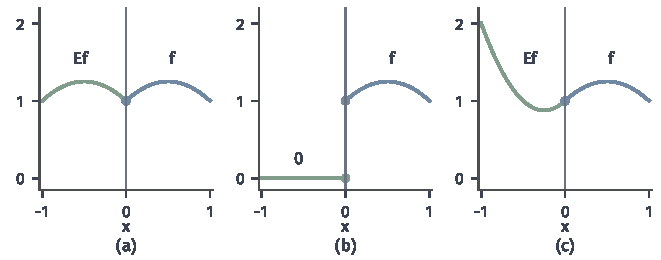
\includegraphics[width=112mm]{figures/04-spaces-measures-and-geometry/03-function-spaces/matplotlib/sobolev-reflections/figure.pdf}
  \caption{同一函数$f(x)=1+x-x^2$的三种延拓，蓝色为原函数，绿色为$x<0$一侧补上的部分。(a)偶反射，在原点连续，但有折点，属于$H^1$，一般不属于$H^2$。(b)零延拓，在原点跳跃，不属于$H^1$。(c)二阶反射$Ef(x)=-3f(-x)+4f(-x/2)$，在原点函数值和一阶导数都相接，属于$H^2$。}
  \label{fig:sobolev-reflections}
\end{BookInlineFigure}

\paragraph{半空间上的偶反射}
高维时最简单的边界是超平面。记$\mathbb R^d_+$为$x_d>0$的半空间，点写成$x=(x',x_d)$，其中$x'\in\mathbb R^{d-1}$。设$f$在闭半空间上连续可微、支撑有界，作偶反射
\[
Ef(x',x_d)=f(x',|x_d|).
\]
我们验证它在全空间有弱导数。对$i<d$，反射不涉及$x_i$，在两个半空间内分别分部积分，就得到$\partial_iEf(x',x_d)=(\partial_if)(x',|x_d|)$。

对$i=d$，取测试函数$\varphi\in C_c^\infty(\mathbb R^d)$，固定$x'$，分别在$x_d>0$和$x_d<0$上对$x_d$分部积分：
\[
\begin{aligned}
\int_0^\infty f(x',t)\,\partial_d\varphi\,\mathrm dt
&=-f(x',0)\varphi(x',0)-\int_0^\infty\partial_df\,\varphi\,\mathrm dt,\\
\int_{-\infty}^0 f(x',-t)\,\partial_d\varphi\,\mathrm dt
&=f(x',0)\varphi(x',0)+\int_{-\infty}^0(\partial_df)(x',-t)\,\varphi\,\mathrm dt .
\end{aligned}
\]
第二式用了链式法则：$t\mapsto f(x',-t)$的导数是$-(\partial_df)(x',-t)$。

两式相加，边界面上的项$\pm f(x',0)\varphi(x',0)$恰好相消。再对$x'$积分，得
\[
\int_{\mathbb R^d}Ef\,\partial_d\varphi\,\mathrm dx
=-\int_{\mathbb R^d}\operatorname{sgn}(x_d)\,(\partial_df)(x',|x_d|)\,\varphi\,\mathrm dx .
\]
所以
\[
\partial_dEf=\operatorname{sgn}(x_d)\,(\partial_df)(x',|x_d|).
\]
两侧对称，范数恒等式与式~\eqref{eq:sobolev-reflection-norm}相同：全空间上的$p$次方范数是半空间上的两倍。

上面的计算要求$f$光滑到边界并且支撑有界，一般的$f\in W^{1,p}(\mathbb R^d_+)$（$1\leq p<\infty$）可以这样逼近。先用$\chi(x/R)$截断，由引理~\ref{lem:sobolev-product-rule}和控制收敛，$R\to\infty$时误差趋于零。再向内部平移，$f_h(x',x_d)=f(x',x_d+h)$在更大的半空间$x_d>-h$上有定义，用半径小于$h$的磨光，就得到在闭半空间上光滑、支撑有界的函数。令$h$与磨光半径趋于零，由平移的积分连续性和磨光收敛，这些函数在$W^{1,p}(\mathbb R^d_+)$中趋于截断后的函数。

于是$E$在一个稠密子空间上满足上述范数恒等式。由$W^{1,p}(\mathbb R^d)$的完备性，它唯一地延伸为整个$W^{1,p}(\mathbb R^d_+)$上的有界线性算子，延伸后的$Ef$仍几乎处处等于$f(x',|x_d|)$。

\paragraph{零延拓与边界相容条件}
与偶反射对照，把$f$在$x_d<0$处直接补成零，称为\term{零延拓}（zero extension）。重做上面的分部积分，只剩$x_d>0$一侧，边界项
\[
-\int_{\mathbb R^{d-1}}f(x',0)\,\varphi(x',0)\,\mathrm dx'
\]
不再被抵消。若$f$在边界面上的值不恒为零，这一项集中在零测的超平面上，不能写成$\int g\varphi$的形式，论证与阶跃函数相同。图~\ref{fig:sobolev-reflections}的(b)是一维的情形：跳跃出现在接缝处，$(0,1)$上的常数$1$零延拓后就是阶跃函数，不属于$W^{1,p}(-1,1)$。

所以零延拓需要边界相容条件：函数在边界上的值为零。对光滑到边界的函数，这一条件可以逐点检查。对一般的Sobolev函数，“边界值”要通过第~\ref{sec:sobolev-trace}小节的迹来理解。第~\ref{sec:sobolev-compact-closure}小节的闭包空间恰好由这类函数组成，零延拓在其上保持范数不变。

\paragraph{高阶延拓}
偶反射对$W^{2,p}$不够。反射后$\partial_dEf$在$x_d>0$一侧趋于$\partial_df(x',0)$，在另一侧趋于$-\partial_df(x',0)$。只要法向导数在边界上不为零，$\partial_dEf$就有跳跃，没有局部可积的弱导数。高阶延拓必须让函数及其直到$k-1$阶的法向导数在边界两侧相接。

对$k=2$，可以在$x_d<0$处令
\begin{equation}
Ef(x',x_d)=-3f(x',-x_d)+4f\Bigl(x',-\frac{x_d}{2}\Bigr).
\label{eq:sobolev-second-order-reflection}
\end{equation}
系数的选取是为了让两个条件同时成立。在$x_d=0$处，函数值为$-3f+4f=f(x',0)$。对$x_d$求导，得到
\[
\partial_dEf(x',x_d)=3\,\partial_df(x',-x_d)-2\,\partial_df\Bigl(x',-\frac{x_d}2\Bigr),
\]
它在边界上等于$\partial_df(x',0)$。

用图~\ref{fig:sobolev-reflections}(c)的函数手算核对。$f(x)=1+x-x^2$代入式~\eqref{eq:sobolev-second-order-reflection}，$x<0$时得
\[
Ef(x)=-3(1-x-x^2)+4\Bigl(1-\frac x2-\frac{x^2}4\Bigr)=1+x+2x^2 .
\]
在$x=0$处函数值都是$1$，一阶导数都是$1$。二阶导数左侧是$4$，右侧是$-2$，有跳跃，但二阶导数只需要作为$L^p$函数存在。

一般地，$Ef$在全空间连续可微，两侧分别二阶光滑，按前面的分部积分，二阶弱导数存在且局部可积。$x_d<0$一侧的各阶导数是$f$的导数在两个缩放位置的有限组合，换元后得到
\[
\lVert Ef\rVert_{W^{2,p}(\mathbb R^d)}\leq C\lVert f\rVert_{W^{2,p}(\mathbb R^d_+)} .
\]
对一般的$k$，取$k$个系数使前$k$个法向导数都相接即可。

\paragraph{Lipschitz区域}
一般区域的边界可以弯曲，甚至有棱角。只要边界在每点附近都能写成函数图像，并且区域只位于图像的一侧，就可以在局部把边界拉直，再用反射。

\begin{definition}[Lipschitz区域]
\label{def:sobolev-lipschitz-domain}
称有界开集$\Omega\subset\mathbb R^d$为\term{Lipschitz区域}（Lipschitz domain），若对每个$x_0\in\partial\Omega$，存在$r>0$、经旋转与平移得到的坐标$(x',x_d)$以及Lipschitz函数$\gamma:\mathbb R^{d-1}\to\mathbb R$，使
\begin{equation}
\Omega\cap B(x_0,r)=\{x\in B(x_0,r):x_d>\gamma(x')\}.
\label{eq:sobolev-lipschitz-graph}
\end{equation}
\end{definition}

图~\ref{fig:sobolev-lipschitz-domains}对比了三种情形。球、立方体和有界凸开集都是Lipschitz区域；立方体在棱角处不光滑，但把坐标轴转过去，局部仍是Lipschitz图像。挖去一条线段的圆盘不是：割缝两侧都属于区域，区域不能只位于割缝的一侧。

\begin{BookInlineFigure}
  \centering
  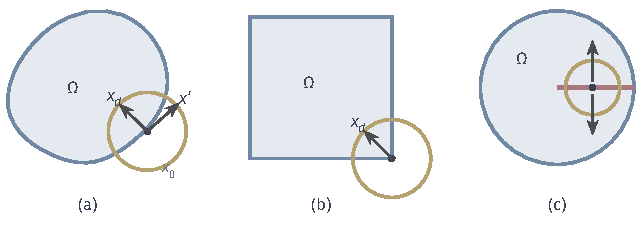
\includegraphics[width=108.356mm]{figures/04-spaces-measures-and-geometry/03-function-spaces/tikz/sobolev-lipschitz-domains/figure.pdf}
  \caption{Lipschitz区域的局部图像条件，黄圈为球$B(x_0,r)$。(a)弯曲边界，局部坐标中$x_d$指向区域内，$\Omega$位于图像$x_d=\gamma(x')$的上方。(b)方形的角点，把$x_d$轴转到对角线方向后，边界仍是Lipschitz图像。(c)割缝圆盘，红线为割缝，黄圈内区域同时位于割缝两侧，不能写成单侧图像，因而不是Lipschitz区域。}
  \label{fig:sobolev-lipschitz-domains}
\end{BookInlineFigure}

\begin{theorem}[Lipschitz区域上的延拓]
\label{thm:sobolev-extension}
设$\Omega\subset\mathbb R^d$为有界Lipschitz区域，$1\leq p<\infty$。存在有界线性算子$E:W^{1,p}(\Omega)\to W^{1,p}(\mathbb R^d)$和有界集合$B_\Omega$，使对每个$f\in W^{1,p}(\Omega)$，$Ef$在$\Omega$上几乎处处等于$f$，并且$Ef$在$B_\Omega$之外为零。
\end{theorem}

完整证明要处理Lipschitz变换下的弱导数，篇幅较长，读者可查阅Sobolev空间的专著，这里说明构造的步骤。边界是紧集，可以用有限个满足定义的球覆盖，再加上一个闭包含于$\Omega$的开集覆盖内部。取从属于这有限个开集的单位分解，把$f$分成有限块，内部那块在边界附近为零，直接零延拓。

每个边界块用变换$(x',x_d)\mapsto(x',x_d-\gamma(x'))$拉直为半空间上的函数，作偶反射，再变换回去。这个变换与它的逆都是Lipschitz映射，它们把$W^{1,p}$函数映为$W^{1,p}$函数，范数只相差由$\gamma$的Lipschitz常数决定的倍数。最后用一个固定的截断函数乘以和式，使所有延拓都在同一有界集合外为零。

这一构造对一阶空间有效，但不能直接推广到高阶：Lipschitz拉直变换只有一阶导数的控制，复合以后二阶导数一般不存在。若边界是$C^k$图像，可以用光滑的拉直变换配合上面的高阶反射。对一般有界Lipschitz区域，$W^{k,p}$的延拓也存在，但需要不同的构造，读者可查阅相关专著。

\paragraph{光滑到边界的逼近}
延拓定理的一个直接推论是更强的逼近：逼近函数可以取为全空间紧支撑光滑函数在$\Omega$上的限制，从而连同各阶导数都连续到边界。

\begin{theorem}[光滑到边界的逼近]
\label{thm:sobolev-smooth-up-to-boundary}
设$\Omega$为有界Lipschitz区域，$1\leq p<\infty$。则$\{\psi|_\Omega:\psi\in C_c^\infty(\mathbb R^d)\}$在$W^{1,p}(\Omega)$中稠密。
\end{theorem}

\begin{proof}
对$f\in W^{1,p}(\Omega)$，由定理~\ref{thm:sobolev-extension}得到在有界集合外为零的$Ef\in W^{1,p}(\mathbb R^d)$。$Ef*\rho_\varepsilon$光滑且支撑紧，由式~\eqref{eq:sobolev-whole-space-mollify}，它在$W^{1,p}(\mathbb R^d)$中趋于$Ef$。限制到$\Omega$上范数只会变小，所以
\[
\lVert(Ef*\rho_\varepsilon)|_\Omega-f\rVert_{W^{1,p}(\Omega)}
\leq\lVert Ef*\rho_\varepsilon-Ef\rVert_{W^{1,p}(\mathbb R^d)}\to0.
\qedhere
\]
\end{proof}

记这类限制函数的全体为$C^\infty(\overline\Omega)$。与定理~\ref{thm:sobolev-meyers-serrin}相比，这里多了边界正则性的假设，换来的是光滑到边界的逼近函数。下一节定义边界值时，正是先对这类函数直接限制到边界，再用逼近推广到整个空间。

\section{约束子空间}
\label{sec:sobolev-constrained-subspaces}

许多问题要求函数满足边界条件，例如在区间两端取零，或在区域边界上取指定的值。Sobolev函数是几乎处处等价类，而边界是零测集，任意修改边界上的值不改变元素，所以“边界值”不能取一个代表直接读出。本节先用紧支撑光滑函数的闭包定义零边界子空间，它不涉及任何边界值；再在一维用绝对连续代表读出端点值，在高维用迹映射表达边界值。最后研究零边界与零均值约束怎样排除常数方向，使导数单独给出等价范数。

\subsection{紧支撑光滑函数的闭包}
\label{sec:sobolev-compact-closure}

紧支撑光滑函数在边界附近恒为零。若一个Sobolev函数能被这样的函数在Sobolev范数下任意逼近，它就在极限意义上“在边界附近为零”。把这一想法直接取作定义。

\begin{definition}[零边界Sobolev空间]
\label{def:sobolev-w0}
设$\Omega\subset\mathbb R^d$为开集，$k\geq1$为整数，$1\leq p<\infty$。把$C_c^\infty(\Omega)$在$W^{k,p}(\Omega)$范数下的闭包记作$W_0^{k,p}(\Omega)$，称为\term{零边界Sobolev空间}（Sobolev space with zero boundary values），$p=2$时记作$H_0^k(\Omega)$。
\end{definition}

这里的闭包是第~\ref{chap:topological-spaces}章的概念：在由Sobolev范数给出的度量下，每个邻域都与$C_c^\infty(\Omega)$相交的元素全体。度量空间中，它恰好由$C_c^\infty(\Omega)$中序列的极限组成。若$\varphi_n\to f$、$\psi_n\to g$，则对实数$a,b$有$a\varphi_n+b\psi_n\to af+bg$，而$a\varphi_n+b\psi_n$仍是紧支撑光滑函数，所以闭包对线性组合封闭。闭包本身是闭集，于是$W_0^{k,p}(\Omega)$是$W^{k,p}(\Omega)$的闭线性子空间，由定理~\ref{thm:sobolev-complete}，它本身也是Banach空间。

定义只用到逼近，不需要区域边界的任何正则性。两个问题需要分别核对。第一，$W_0^{k,p}(\Omega)$一般是真子空间，下一小节将证明$(0,1)$上的常数$1$不属于$H_0^1(0,1)$。在全空间则没有边界：取在$|x|\leq1$上为$1$、在$|x|\geq2$外为零的截断函数$\chi$，$\chi(x/R)f$在$R\to\infty$时于$W^{k,p}(\mathbb R^d)$中趋于$f$，再对它磨光，可知$W_0^{k,p}(\mathbb R^d)=W^{k,p}(\mathbb R^d)$。第二，定义限于$p<\infty$。在$W^{1,\infty}$范数下，紧支撑光滑函数的极限具有一致连续的导数，第~\ref{sec:sobolev-smooth-density}节末尾的$|x-1/2|$与之距离至少为$1$；所以$p=\infty$时的闭包远小于“零边界的$W^{1,\infty}$函数”，有限指数的结论不能照搬。

\subsection{端点值}
\label{sec:sobolev-endpoint-values}

一维时，边界只有两个端点，而第~\ref{chap:smoothing-weak-derivatives}章已经证明$v\in H^1(0,1)$有绝对连续代表$\tilde v$，并且$\tilde v(y)-\tilde v(x)=\int_x^yv'(t)\,\mathrm dt$。端点值$\tilde v(0)$与$\tilde v(1)$由这个代表确定。我们需要知道它们是否受$H^1$范数控制。

把上式对$x\in(0,1)$积分。由于区间长度为$1$，
\[
\tilde v(y)=\int_0^1\tilde v(x)\,\mathrm dx+\int_0^1\int_x^yv'(t)\,\mathrm dt\,\mathrm dx,\qquad
|\tilde v(y)|\leq\int_0^1|v|\,\mathrm dx+\int_0^1|v'|\,\mathrm dt .
\]
再由Cauchy--Schwarz不等式，$\int_0^1|v|\leq\lVert v\rVert_2$，$\int_0^1|v'|\leq\lVert v'\rVert_2$。于是对每个$y\in[0,1]$，特别是两个端点，
\begin{equation}
|\tilde v(y)|\leq\lVert v\rVert_2+\lVert v'\rVert_2\leq\sqrt2\,\lVert v\rVert_{H^1(0,1)} .
\label{eq:sobolev-endpoint-bound}
\end{equation}
所以映射$v\mapsto\tilde v(0)$是线性的，并且对$H^1$范数连续；$v\mapsto\tilde v(1)$同理。式\eqref{eq:sobolev-endpoint-bound}还说明，$H^1$收敛蕴含连续代表的一致收敛。

只有$L^2$控制是不够的。$v_n(x)=\max(1-nx,0)$满足$v_n(0)=1$，而$\lVert v_n\rVert_2^2=\int_0^{1/n}(1-nx)^2\,\mathrm dx=1/(3n)\to0$。端点值能被控制，靠的是导数项：$\lVert v_n'\rVert_2=\sqrt n$随$n$增大。

现在把估计用于闭包。每个$\varphi\in C_c^\infty(0,1)$在端点为零。若$\varphi_n\to v$在$H^1$中成立，由式\eqref{eq:sobolev-endpoint-bound}，$\tilde v(0)=\lim\varphi_n(0)=0$，同理$\tilde v(1)=0$。所以$H_0^1(0,1)=W_0^{1,2}(0,1)$中的函数都有零端点值。常数$1$不满足这一条件，并且对每个$\varphi\in C_c^\infty(0,1)$，
\[
1=|1-\varphi(0)|\leq\sqrt2\,\lVert1-\varphi\rVert_{H^1},
\]
它到紧支撑光滑函数的$H^1$距离至少是$1/\sqrt2$。反过来，连续代表在两端为零的$H^1(0,1)$函数都属于$H_0^1(0,1)$，这是下一小节零迹刻画在一维的情形。

\subsection{迹映射}
\label{sec:sobolev-trace}

高维时，$W^{1,p}$函数一般没有连续代表，第~\ref{sec:sobolev-continuous-embeddings}节将给出在边界点附近无界的例子，因此不能逐点读取边界值。我们改为先对光滑到边界的函数直接限制到边界，证明限制的边界$L^p$大小受Sobolev范数控制，再用逼近推广。

\paragraph{半空间上的估计}
设$f\in C_c^1(\mathbb R^d)$，考虑它在闭半空间$\overline{\mathbb R^d_+}$上的部分。固定$x'$，沿$x_d$方向从边界点$(x',0)$向内积分。$t$足够大时$f(x',t)=0$，所以$p=1$时
\[
|f(x',0)|=\Bigl|\int_0^\infty\partial_df(x',t)\,\mathrm dt\Bigr|\leq\int_0^\infty|\partial_df(x',t)|\,\mathrm dt .
\]
$p>1$时$|f|^p$连续可微，导数的绝对值不超过$p|f|^{p-1}|\partial_df|$。由Young不等式$ab\leq a^{p'}/p'+b^p/p$（取$a=|f|^{p-1}$，$b=|\partial_df|$，$p'=p/(p-1)$），
\[
|f(x',0)|^p=-\int_0^\infty\partial_t\bigl(|f(x',t)|^p\bigr)\,\mathrm dt\leq\int_0^\infty\bigl((p-1)|f|^p+|\partial_df|^p\bigr)\,\mathrm dt .
\]
两种情形都对$x'\in\mathbb R^{d-1}$积分，得到
\begin{equation}
\int_{\mathbb R^{d-1}}|f(x',0)|^p\,\mathrm dx'\leq\max(p-1,1)\,\lVert f\rVert_{W^{1,p}(\mathbb R^d_+)}^p .
\label{eq:sobolev-half-space-trace}
\end{equation}
边界值的$L^p$大小被体积上函数与法向导数的大小控制。这与端点估计是同一机制：沿垂直于边界的每条直线，问题都是一维的。

\paragraph{Lipschitz区域上的迹}
在有界Lipschitz区域上，边界需要配上\term{表面测度}（surface measure）$\mathrm dS$。在定义~\ref{def:sobolev-lipschitz-domain}的局部图像$x_d=\gamma(x')$上，取$\mathrm dS=\sqrt{1+|\nabla\gamma(x')|^2}\,\mathrm dx'$。Lipschitz函数几乎处处可微且梯度有界，所以这个因子介于$1$与$\sqrt{1+L_\gamma^2}$之间，$L_\gamma$为$\gamma$的Lipschitz常数；不同局部图像在重叠处给出同一测度，这一点这里不加证明地使用。记$L^p(\partial\Omega)=L^p(\partial\Omega,\mathrm dS)$。

\begin{theorem}[迹定理]
\label{thm:sobolev-trace}
设$\Omega\subset\mathbb R^d$为有界Lipschitz区域，$1\leq p<\infty$。存在常数$C$，使所有$f\in C^\infty(\overline\Omega)$满足
\begin{equation}
\lVert f|_{\partial\Omega}\rVert_{L^p(\partial\Omega)}\leq C\lVert f\rVert_{W^{1,p}(\Omega)} .
\label{eq:sobolev-trace-inequality}
\end{equation}
并且存在唯一的有界线性算子$\operatorname{Tr}:W^{1,p}(\Omega)\to L^p(\partial\Omega)$，使$\operatorname{Tr}f=f|_{\partial\Omega}$对所有$f\in C^\infty(\overline\Omega)$成立。
\end{theorem}

不等式\eqref{eq:sobolev-trace-inequality}的证明思路与延拓定理相同：用有限个边界球和一个内部开集覆盖$\overline\Omega$，取从属的单位分解把$f$分成有限块；内部那块在边界上为零；每个边界块经拉直变成半空间上的紧支撑函数，套用式\eqref{eq:sobolev-half-space-trace}，再把拉直变换与表面测度因子带来的有界倍数计入常数。这里不给出细节。

\begin{proof}[算子的构造]
设不等式\eqref{eq:sobolev-trace-inequality}成立。对$f\in W^{1,p}(\Omega)$，由定理~\ref{thm:sobolev-smooth-up-to-boundary}取$f_n\in C^\infty(\overline\Omega)$在$W^{1,p}$中趋于$f$。由式\eqref{eq:sobolev-trace-inequality}，
\[
\lVert f_n|_{\partial\Omega}-f_m|_{\partial\Omega}\rVert_{L^p(\partial\Omega)}\leq C\lVert f_n-f_m\rVert_{W^{1,p}(\Omega)},
\]
所以边界限制在$L^p(\partial\Omega)$中构成Cauchy列，收敛到某个$g$。若$h_n$是另一个逼近列，交错排列的$(f_1,h_1,f_2,h_2,\ldots)$仍趋于$f$，其边界限制也收敛，于是两个子列的极限相同，$g$不依赖逼近列。令$\operatorname{Tr}f=g$。线性由极限的线性得到，$\lVert\operatorname{Tr}f\rVert_{L^p(\partial\Omega)}\leq C\lVert f\rVert_{W^{1,p}}$由不等式取极限得到。两个有界线性算子若在稠密子集上相同，便处处相同，这给出唯一性。
\end{proof}

称$\operatorname{Tr}f$为$f$的\term{边界迹}（boundary trace）。它是$L^p(\partial\Omega)$中的等价类，而不是任选一个代表后逐点读出的边界值：修改$f$在零测集$\partial\Omega$上的值不改变$f$，也不改变$\operatorname{Tr}f$；修改代表在区域内部某个零测集上的值同样不影响它。迹由“函数在靠近边界处的平均行为”决定，这正是逼近构造所表达的。

零迹与零边界子空间在一阶情形可以对应起来。$C_c^\infty(\Omega)$中的函数在边界附近为零，迹为零；$\operatorname{Tr}$连续，零迹在$W^{1,p}$极限下保持，所以$W_0^{1,p}(\Omega)\subset\ker\operatorname{Tr}$。反向包含在有界Lipschitz区域上也成立，因而
\[
W_0^{1,p}(\Omega)=\{f\in W^{1,p}(\Omega):\operatorname{Tr}f=0\}.
\]
反向包含的证明思路是：在每个局部图像中把零迹函数沿远离边界的方向推进一小段，乘以在边界附近为零的截断函数，再磨光；零迹保证截断造成的误差随推进距离趋于零。这里不给出细节。

这一对应不能直接推广为高阶零迹的完整刻画。在$(0,1)$上取$f(x)=x(1-x)\in H^2(0,1)$，它的端点值为零，但$f'(0)=1$。对$\varphi\in C_c^\infty(0,1)$，把式\eqref{eq:sobolev-endpoint-bound}用于$(f-\varphi)'$，得$1=|f'(0)-\varphi'(0)|\leq\sqrt2\lVert f-\varphi\rVert_{H^2}$，所以$f\notin H_0^2(0,1)$。高阶闭包还要求法向导数的边界值为零，刻画它需要对导数的迹另作讨论。

\subsection{约束子空间中的导数范数}
\label{sec:sobolev-derivative-norms}

第~\ref{sec:sobolev-oscillation}小节指出，常数的导数为零，因此在整个$W^{1,p}(\Omega)$上，导数的大小不能控制函数本身。记$|\nabla f|$为弱梯度$(\partial_1f,\ldots,\partial_df)$的欧氏长度，$\lVert\nabla f\rVert_p$为它的$L^p$范数。逐点有$|\partial_if|\leq|\nabla f|\leq\sum_i|\partial_if|$，所以$\lVert\nabla f\rVert_p$与$(\sum_i\lVert\partial_if\rVert_p^p)^{1/p}$只相差依赖$d,p$的倍数。我们要回答：在排除常数方向的子空间上，是否存在常数$C$使$\lVert f\rVert_p\leq C\lVert\nabla f\rVert_p$。零边界与零均值是两种排除常数的方式。

\paragraph{零边界情形}
形如$\lVert f\rVert_p\leq C\lVert\nabla f\rVert_p$的估计称为\term{Poincaré不等式}（Poincaré inequality）。零边界条件下，它不需要区域连通或边界正则，只需要区域在一个方向上有界。

\begin{theorem}[零边界的Poincaré不等式]
\label{thm:sobolev-poincare-zero}
设$\Omega\subset\mathbb R^d$为开集，含于带状区域$\{x:a<x_1<a+L\}$，$1\leq p<\infty$。则对所有$f\in W_0^{1,p}(\Omega)$，
\[
\lVert f\rVert_p\leq\frac{L}{p^{1/p}}\lVert\partial_1f\rVert_p\leq\frac{L}{p^{1/p}}\lVert\nabla f\rVert_p .
\]
\end{theorem}

\begin{proof}
先设$f\in C_c^\infty(\Omega)$，并把它在$\Omega$外补成零。记$x=(x_1,x'')$。由于$f(a,x'')=0$，
\begin{equation*}
\begin{aligned}
|f(x_1,x'')|&=\Bigl|\int_a^{x_1}\partial_1f(t,x'')\,\mathrm dt\Bigr|\\
&\leq(x_1-a)^{1-1/p}\Bigl(\int_a^{a+L}|\partial_1f(t,x'')|^p\,\mathrm dt\Bigr)^{1/p},
\end{aligned}
\end{equation*}
第二步是Hölder不等式。取$p$次方，对$x_1\in(a,a+L)$积分，$\int_a^{a+L}(x_1-a)^{p-1}\,\mathrm dx_1=L^p/p$；再对$x''$积分，得$\lVert f\rVert_p^p\leq(L^p/p)\lVert\partial_1f\rVert_p^p$。两边都对$W^{1,p}$范数连续，由$W_0^{1,p}(\Omega)$的定义取极限即得一般情形。
\end{proof}

\paragraph{零均值情形}
零均值$f_\Omega=|\Omega|^{-1}\int_\Omega f\,\mathrm dx=0$同样排除了非零常数，但它是整体条件，需要区域连通，否则可以在不同分支上取不同常数。我们先在凸区域上用积分估计完整证明，再说明一般区域怎样局部拼接。下面的引理用一点的值与区域平均之差来读取梯度的作用。

\begin{lemma}[凸区域上的平均估计]
\label{lem:sobolev-convex-average}
设$W\subset\mathbb R^d$为有界凸开集，直径为$D$，$f$在$\overline W$的一个邻域上连续可微。则对每个$x\in\overline W$，
\begin{equation}
|f(x)-f_W|\leq\frac{D^d}{d\,|W|}\int_W\frac{|\nabla f(z)|}{|x-z|^{d-1}}\,\mathrm dz .
\label{eq:sobolev-convex-average}
\end{equation}
\end{lemma}

\begin{proof}
对$y\in W$，记$\omega=(y-x)/|y-x|$。凸性保证除端点$x$外，线段$[x,y]$都落在$W$中，所以$|f(y)-f(x)|\leq\int_0^{|y-x|}G(x+t\omega)\,\mathrm dt$，其中$G=|\nabla f|\mathbf 1_W$。由$f(x)-f_W=|W|^{-1}\int_W(f(x)-f(y))\,\mathrm dy$，
\[
|f(x)-f_W|\leq\frac1{|W|}\int_W\int_0^\infty G(x+t\omega)\,\mathrm dt\,\mathrm dy .
\]
以$x$为中心用球坐标$y=x+\rho\omega$，$\mathrm dy=\rho^{d-1}\mathrm d\rho\,\mathrm d\sigma(\omega)$，$\rho\leq D$。内层积分只依赖方向$\omega$，对$\rho$积分给出因子$D^d/d$。剩下的$\int_{S^{d-1}}\int_0^\infty G(x+t\omega)\,\mathrm dt\,\mathrm d\sigma(\omega)$再按球坐标还原为$\int G(z)|z-x|^{1-d}\,\mathrm dz$，即得式\eqref{eq:sobolev-convex-average}。
\end{proof}

\begin{theorem}[凸区域上的零均值Poincaré不等式]
\label{thm:sobolev-poincare-convex}
设$W\subset\mathbb R^d$为有界凸开集，直径为$D$，$1\leq p<\infty$。则对所有$f\in W^{1,p}(W)$，
\[
\lVert f-f_W\rVert_p\leq\frac{|B(0,D)|}{|W|}\,D\,\lVert\nabla f\rVert_p .
\]
\end{theorem}

\begin{proof}
先设$f\in C^\infty(\overline W)$。记$Tg(x)=\int_W g(z)|x-z|^{1-d}\,\mathrm dz$。对每个$x\in W$，$W\subset B(x,D)$，所以$\int_W|x-z|^{1-d}\,\mathrm dz\leq\int_{B(x,D)}|x-z|^{1-d}\,\mathrm dz=|S^{d-1}|D$，其中$|S^{d-1}|$为单位球面的面积；对$z$固定、$x$变化也一样。把核写成$|x-z|^{(1-d)/p'}\cdot|x-z|^{(1-d)/p}$，用Hölder不等式，
\[
|Tg(x)|^p\leq\bigl(|S^{d-1}|D\bigr)^{p-1}\int_W|g(z)|^p|x-z|^{1-d}\,\mathrm dz ,
\]
再对$x$积分并交换积分次序，得$\lVert Tg\rVert_p\leq|S^{d-1}|D\,\lVert g\rVert_p$。把它与式\eqref{eq:sobolev-convex-average}合并，并用$|B(0,D)|=|S^{d-1}|D^d/d$，即得所需估计。有界凸开集是Lipschitz区域，由定理~\ref{thm:sobolev-smooth-up-to-boundary}，$C^\infty(\overline W)$在$W^{1,p}(W)$中稠密；均值满足$|f_W-g_W|\leq|W|^{-1/p}\lVert f-g\rVert_p$，两边都对$W^{1,p}$范数连续，取极限得一般情形。
\end{proof}

对一般的有界连通Lipschitz区域$\Omega$，零均值的Poincaré不等式$\lVert f-f_\Omega\rVert_p\leq C\lVert\nabla f\rVert_p$同样成立，$1\leq p<\infty$，常数依赖$\Omega$与$p$。局部拼接的思路如下：用有限个已有局部估计的小区域覆盖$\Omega$，内部用球，边界附近用拉直后的柱形区域；连通性保证任意两块能由一串依次重叠的小区域相连，重叠部分测度为正，于是相邻两块均值之差被梯度控制，逐块传递得到整体估计。这里不给出完整证明。第~\ref{sec:sobolev-compact-lq}小节的紧嵌入还给出另一条路线：若估计不成立，可取$\lVert f_n\rVert_p=1$、均值为零、$\lVert\nabla f_n\rVert_p\to0$的序列，紧嵌入给出$L^p$收敛子列，其极限梯度为零，在连通区域上只能是常数，零均值迫使它为零，与范数为$1$矛盾。

\paragraph{条件为什么不能少}
连通性不能去掉：在$(0,1)\cup(2,3)$上，第一段取$-1$、第二段取$1$的函数均值为零、弱导数为零，却不是零。约束不能去掉：常数函数本身就是反例。零边界情形中区域有界的方向也不能去掉：在$\mathbb R$上取非零$\psi\in C_c^\infty(\mathbb R)$，令$\psi_R(x)=\psi(x/R)$，则$\lVert\psi_R\rVert_2=R^{1/2}\lVert\psi\rVert_2$，$\lVert\psi_R'\rVert_2=R^{-1/2}\lVert\psi'\rVert_2$，比值随$R$无界。

\paragraph{导数给出的等价范数}
Poincaré不等式把约束和导数范数联系起来。在定理~\ref{thm:sobolev-poincare-zero}的条件下，对$f\in W_0^{1,p}(\Omega)$，
\[
\frac{1}{d^{1-1/p}}\lVert\nabla f\rVert_p\leq\lVert f\rVert_{W^{1,p}}\leq\Bigl(\frac{L^p}{p}+d\Bigr)^{1/p}\lVert\nabla f\rVert_p .
\]
左边来自$\lVert\nabla f\rVert_p\leq\sum_i\lVert\partial_if\rVert_p$与$\ell^p$、$\ell^1$范数的比较，右边来自Poincaré不等式与$|\partial_if|\leq|\nabla f|$。于是在零边界子空间上，$\lVert\nabla f\rVert_p$就是一个等价范数；$p=2$时，$\int_\Omega\nabla f\cdot\nabla g$是$H_0^1(\Omega)$上与原内积等价的内积。在连通Lipschitz区域的零均值子空间上，结论相同。在整个$W^{1,p}(\Omega)$上则不行，二者的差别恰好是常数方向。

\section{连续嵌入}
\label{sec:sobolev-continuous-embeddings}

一维时，第~\ref{chap:smoothing-weak-derivatives}章已经证明$W^{1,1}$函数有绝对连续代表，所以有界。高维时情况不同：导数可积能把函数本身控制到什么程度，取决于积分指数$p$与维数$d$的关系。本节固定有界Lipschitz区域$\Omega\subset\mathbb R^d$，研究一阶Sobolev范数能控制函数在哪些目标空间中的大小。

若包含关系$W^{1,p}(\Omega)\subset Y$连同估计
\begin{equation}
\lVert f\rVert_Y\leq C\lVert f\rVert_{W^{1,p}}
\label{eq:sobolev-continuous-embedding}
\end{equation}
成立，常数$C$不依赖$f$，就称它为\term{连续嵌入}（continuous embedding）：包含映射是有界线性算子。

本节的两个基本条件各有用途。区域有界保证较小指数的$L^q$范数受较大指数控制：对$q\leq r$，由Hölder不等式，
\[
\lVert f\rVert_q\leq|\Omega|^{1/q-1/r}\lVert f\rVert_r .
\]
区域为Lipschitz，保证第~\ref{sec:sobolev-extension}节的延拓和光滑到边界的逼近可用。

\paragraph{缩放决定指数}
在讨论证明以前，先看目标指数应当是多少。设想全空间上的光滑紧支撑函数满足$\lVert u\rVert_q\leq C\lVert\nabla u\rVert_p$，$C$不依赖$u$。对$\lambda>0$，令$u_\lambda(x)=u(\lambda x)$，换元$y=\lambda x$给出
\[
\lVert u_\lambda\rVert_q=\lambda^{-d/q}\lVert u\rVert_q,\qquad
\lVert\nabla u_\lambda\rVert_p=\lambda^{1-d/p}\lVert\nabla u\rVert_p .
\]

不等式对所有$\lambda$成立，两边$\lambda$的指数必须相同，否则令$\lambda\to0$或$\lambda\to\infty$就会破坏它。于是$-d/q=1-d/p$，即
\begin{equation}
\frac1{p^*}=\frac1p-\frac1d,\qquad p^*=\frac{dp}{d-p}\quad(1\leq p<d).
\label{eq:sobolev-conjugate-exponent}
\end{equation}
称$p^*$为$p$的\term{Sobolev共轭指数}（Sobolev conjugate exponent）。例如$d=3$、$p=2$时$p^*=6$，缩放指数两边都是$\lambda^{-1/2}$。

缩放只说明指数必须是什么，并没有证明不等式成立。它也显示了维数的作用：$d$越大、$p$越小，把函数压缩到小尺度时导数的$L^p$范数增长得越慢，导数就越难察觉尖锐的集中。

\subsection{更高指数的可积性}
\label{sec:sobolev-higher-integrability}

当$p<d$时，我们证明$W^{1,p}$函数属于比$L^p$更好的$L^{p^*}$。

\begin{theorem}[Sobolev嵌入，$p<d$]
\label{thm:sobolev-embedding-subcritical}
设$d\geq2$，$1\leq p<d$，$\Omega\subset\mathbb R^d$为有界Lipschitz区域。存在常数$C$，使所有$f\in W^{1,p}(\Omega)$满足
\begin{equation}
\lVert f\rVert_{L^{p^*}(\Omega)}\leq C\lVert f\rVert_{W^{1,p}(\Omega)} .
\label{eq:sobolev-embedding-subcritical}
\end{equation}
因而对每个$1\leq q\leq p^*$，把左端换成$\lVert f\rVert_q$后估计仍成立，只需把常数乘以$|\Omega|^{1/q-1/p^*}$。
\end{theorem}

证明分四步：先对全空间紧支撑函数证明$p=1$的情形，再借幂函数推到$p>1$，然后用逼近推广到$W^{1,p}(\mathbb R^d)$，最后用延拓回到区域。

\paragraph{第一步：\texorpdfstring{$p=1$}{p=1}的全空间估计}
设$u\in C_c^1(\mathbb R^d)$。沿第$i$个坐标方向，从$-\infty$积分到$x_i$，得到
\[
|u(x)|\leq g_i(\hat x_i):=\int_{\mathbb R}|\partial_iu|\,\mathrm dx_i ,
\]
其中$\hat x_i$表示去掉第$i$个坐标后的变量，右端不依赖$x_i$。这里每个坐标方向都给了一个上界。

先看$d=2$。此时$|u(x)|^2\leq g_1(x_2)g_2(x_1)$，右端是两个单变量函数之积，对$x_1,x_2$积分后分离：
\[
\int_{\mathbb R^2}|u|^2\,\mathrm dx\leq\Bigl(\int g_1\Bigr)\Bigl(\int g_2\Bigr)=\lVert\partial_1u\rVert_1\lVert\partial_2u\rVert_1 .
\]
于是$\lVert u\rVert_2\leq\lVert\nabla u\rVert_1$，这正是$d=2$、$p=1$、$p^*=2$的情形。

一般维数需要一个把$d$个“各少一个变量”的函数之积分离开的不等式。

\begin{lemma}[分离变量的乘积估计]
\label{lem:sobolev-loomis-whitney}
设$d\geq2$，$h_1,\ldots,h_d$是$\mathbb R^{d-1}$上的非负可测函数，$h_i$的自变量是$\hat x_i$。则
\begin{equation}
\int_{\mathbb R^d}\prod_{i=1}^dh_i(\hat x_i)\,\mathrm dx\leq\prod_{i=1}^d\lVert h_i\rVert_{L^{d-1}(\mathbb R^{d-1})} .
\label{eq:sobolev-loomis-whitney}
\end{equation}
\end{lemma}

\begin{proof}
对维数归纳。$d=2$时，积分直接分离：
\[
\int_{\mathbb R^2}h_1(x_2)\,h_2(x_1)\,\mathrm dx=\lVert h_1\rVert_1\lVert h_2\rVert_1 .
\]

设维数$d\geq2$时成立，考虑$\mathbb R^{d+1}$上的$h_1,\ldots,h_{d+1}$。记最后一个变量为$s$，其余变量为$x'\in\mathbb R^d$，则$h_{d+1}=h_{d+1}(x')$不依赖$s$。固定$s$，对$x'$积分，用指数$d$和$d/(d-1)$的Hölder不等式，得
\[
\int\prod_{i=1}^{d+1}h_i\,\mathrm dx'
\leq\lVert h_{d+1}\rVert_{L^d}\Bigl(\int\prod_{i=1}^dh_i^{d/(d-1)}\,\mathrm dx'\Bigr)^{(d-1)/d}.
\]

对括号内的积分用归纳假设，函数换成$h_i^{d/(d-1)}$。记$A_i(s)=\int h_i(\cdot,s)^d$，积分对$h_i$的其余$d-1$个变量进行。归纳假设给出
\[
\Bigl(\int\prod_{i=1}^dh_i^{d/(d-1)}\,\mathrm dx'\Bigr)^{(d-1)/d}\leq\prod_{i=1}^dA_i(s)^{1/d}.
\]

最后对$s$积分，用$d$个指数都等于$d$的推广Hölder不等式：
\[
\int\prod_{i=1}^dA_i(s)^{1/d}\,\mathrm ds\leq\prod_{i=1}^d\Bigl(\int A_i(s)\,\mathrm ds\Bigr)^{1/d}=\prod_{i=1}^d\lVert h_i\rVert_{L^d(\mathbb R^d)} .
\]
三式合起来，就是维数$d+1$时的结论。
\end{proof}

回到估计。把$d$个坐标方向的界相乘，再开$d-1$次方，得到
\[
|u(x)|^{d/(d-1)}\leq\prod_{i=1}^dg_i(\hat x_i)^{1/(d-1)} .
\]
对$h_i=g_i^{1/(d-1)}$用引理~\ref{lem:sobolev-loomis-whitney}。按$g_i$的定义，
\[
\lVert h_i\rVert_{d-1}^{d-1}=\int g_i\,\mathrm d\hat x_i=\lVert\partial_iu\rVert_1,
\]
所以
\[
\int_{\mathbb R^d}|u|^{d/(d-1)}\,\mathrm dx\leq\prod_{i=1}^d\lVert\partial_iu\rVert_1^{1/(d-1)} .
\]
两边开$(d-1)/d$次方，得到
\begin{equation}
\lVert u\rVert_{d/(d-1)}\leq\prod_{i=1}^d\lVert\partial_iu\rVert_1^{1/d}\leq\lVert\nabla u\rVert_1 .
\label{eq:sobolev-gagliardo-nirenberg}
\end{equation}

\paragraph{第二步：\texorpdfstring{$1<p<d$}{1<p<d}}
对$u\in C_c^1(\mathbb R^d)$和$\gamma>1$，$|u|^\gamma$仍是紧支撑的连续可微函数，梯度满足
\[
\bigl|\nabla|u|^\gamma\bigr|\leq\gamma|u|^{\gamma-1}|\nabla u| .
\]
把式~\eqref{eq:sobolev-gagliardo-nirenberg}用于$|u|^\gamma$，再对右端用Hölder不等式，
\[
\lVert u\rVert_{\gamma d/(d-1)}^\gamma
\leq\gamma\int|u|^{\gamma-1}|\nabla u|\,\mathrm dx
\leq\gamma\lVert u\rVert_{(\gamma-1)p'}^{\gamma-1}\lVert\nabla u\rVert_p .
\]

选择$\gamma=p(d-1)/(d-p)$，让两侧出现同一个范数。逐项核对：
\[
\frac{\gamma d}{d-1}=\frac{dp}{d-p}=p^*,\qquad
(\gamma-1)p'=\frac{d(p-1)}{d-p}\cdot\frac p{p-1}=p^*.
\]
$u$紧支撑，$\lVert u\rVert_{p^*}$有限，若不为零就可以约去$\gamma-1$次方，得到
\begin{equation}
\lVert u\rVert_{p^*}\leq\gamma\lVert\nabla u\rVert_p,\qquad\gamma=\frac{p(d-1)}{d-p}.
\label{eq:sobolev-gns-p}
\end{equation}
$p=1$时$\gamma=1$，与第一步一致。$d=3$、$p=2$时$\gamma=4$，即$\lVert u\rVert_6\leq4\lVert\nabla u\rVert_2$。

\paragraph{第三步：推广到全空间Sobolev函数}
由第~\ref{sec:sobolev-compact-closure}小节，$C_c^\infty(\mathbb R^d)$在$W^{1,p}(\mathbb R^d)$中稠密。对$u\in W^{1,p}(\mathbb R^d)$取$u_n\in C_c^\infty(\mathbb R^d)$在$W^{1,p}$中趋于$u$，再取子列几乎处处收敛。由Fatou引理与式~\eqref{eq:sobolev-gns-p}，
\[
\lVert u\rVert_{p^*}\leq\liminf_n\lVert u_n\rVert_{p^*}\leq\gamma\lim_n\lVert\nabla u_n\rVert_p=\gamma\lVert\nabla u\rVert_p .
\]

\paragraph{第四步：回到区域}
对$f\in W^{1,p}(\Omega)$，用定理~\ref{thm:sobolev-extension}的延拓$Ef$。比较$\ell^1$与$\ell^p$范数，把梯度的范数换成Sobolev范数，会带来因子$d^{1-1/p}$，于是
\[
\lVert f\rVert_{L^{p^*}(\Omega)}\leq\lVert Ef\rVert_{L^{p^*}(\mathbb R^d)}
\leq\gamma\,d^{1-1/p}\,\lVert E\rVert\,\lVert f\rVert_{W^{1,p}(\Omega)},
\]
其中$\lVert E\rVert$是延拓算子的范数。较小指数由区域有限测度得到，这就证明了定理~\ref{thm:sobolev-embedding-subcritical}。

常数的来源由此清楚：$\gamma$只依赖$d,p$，$\lVert E\rVert$依赖区域与$p$，较小指数还多出$|\Omega|$的幂。它们都不依赖被估计的函数，这正是连续嵌入所要求的统一性。

\begin{example}[幂函数与指数的精确性]
\label{ex:sobolev-power-function}
在单位球$B\subset\mathbb R^d$中取$u(x)=|x|^{-a}$，$a>0$。它在原点之外光滑，$|\nabla u|=a|x|^{-a-1}$。若$a+1<d$，挖去半径为$r$的小球后分部积分，小球面上的边界项不超过
\[
\sup|\varphi|\cdot r^{-a}\cdot|S^{d-1}|\,r^{d-1},
\]
随$r\to0$趋于零，所以经典梯度就是弱梯度。

按球坐标，$|x|^{-b}$在$B$上可积当且仅当$b<d$，因此
\[
u\in L^q(B)\iff aq<d,\qquad u\in W^{1,p}(B)\iff(a+1)p<d .
\]
后一条件即$a<d/p-1=d/p^*$，它恰好是$u\in L^{p^*}(B)$的条件。

对任何$q>p^*$，取$a$满足$d/q\leq a<d/p-1$，便得到$W^{1,p}(B)$中不属于$L^q(B)$的函数，所以$p^*$不能再提高。取$d=3$、$p=2$、$p^*=6$，再取$q=8$与$a=0.4$，逐项核对：
\[
(a+1)p=2.8<3,\qquad 6a=2.4<3,\qquad 8a=3.2\geq3 .
\]
所以这个$u$属于$W^{1,2}(B)$和$L^6(B)$，不属于$L^8(B)$，并且在原点附近无界。可见$p<d$时得到的是更高的可积性，而不是有界性或连续性。
\end{example}

\subsection{临界指数下的可积性}
\label{sec:sobolev-critical-integrability}

当$p\to d$时，$p^*=dp/(d-p)\to\infty$。这提示我们考察$p=d\geq2$时能得到什么。

\begin{theorem}[临界指数的嵌入]
\label{thm:sobolev-embedding-critical}
设$d\geq2$，$\Omega\subset\mathbb R^d$为有界Lipschitz区域。对每个有限的$q\geq1$，存在常数$C_q$，使所有$f\in W^{1,d}(\Omega)$满足
\begin{equation}
\lVert f\rVert_q\leq C_q\lVert f\rVert_{W^{1,d}} .
\label{eq:sobolev-embedding-critical}
\end{equation}
\end{theorem}

\begin{proof}
给定$q$，取$1\leq s<d$足够接近$d$，使$s^*=ds/(d-s)\geq q$。区域有界，由Hölder不等式，
\[
\lVert g\rVert_s\leq|\Omega|^{1/s-1/d}\lVert g\rVert_d
\]
对$f$及其各一阶弱导数成立，所以$W^{1,s}$范数受$W^{1,d}$范数控制。再用定理~\ref{thm:sobolev-embedding-subcritical}于指数$s$即得。
\end{proof}

事实上，$W^{1,d}$函数一般无界。在单位球$B\subset\mathbb R^d$中取$u(x)=\ln\ln(e/|x|)$。记$r=|x|$，$t=\ln(e/r)\geq1$，则$|\nabla u|=1/(rt)$。按球坐标，
\[
\begin{aligned}
\int_B|\nabla u|^d\,\mathrm dx
&=|S^{d-1}|\int_0^1\frac{r^{d-1}}{r^d(\ln(e/r))^d}\,\mathrm dr\\
&=|S^{d-1}|\int_1^\infty t^{-d}\,\mathrm dt=\frac{|S^{d-1}|}{d-1},
\end{aligned}
\]
$d\geq2$时有限。这里用了换元$t=\ln(e/r)$，$\mathrm dt=-\mathrm dr/r$。

$u$本身只以$\ln\ln$的速度增长，属于每个$L^q(B)$。小球面上的边界项不超过
\[
\sup|\varphi|\cdot u(r)\,|S^{d-1}|\,r^{d-1}\to0,
\]
所以经典梯度是弱梯度。于是$u\in W^{1,d}(B)$，却在原点趋于无穷。

这说明不能把式~\eqref{eq:sobolev-conjugate-exponent}在$p=d$处“代入”成$p^*=\infty$。常数$C_q$也不可能关于$q$一致：若$C_q\leq C$对所有$q$成立，由于在有限测度区域上$q\to\infty$时$\lVert f\rVert_q$趋于$\lVert f\rVert_\infty$，就得到
\[
\lVert f\rVert_\infty\leq C\lVert f\rVert_{W^{1,d}},
\]
与这个反例矛盾。临界情形处在两种结论之间：可积性对每个有限指数都成立，有界性却失去了。

\subsection{连续代表}
\label{sec:sobolev-continuous-representatives}

当$p>d$时，导数的控制足以给出逐点的振荡估计。机制是比较一点的值与它附近的平均：引理~\ref{lem:sobolev-convex-average}把这个差写成梯度乘以核$|x-z|^{1-d}$的积分，而这个核的$p'$次幂恰好在$p>d$时局部可积。

\begin{theorem}[Hölder连续代表]
\label{thm:sobolev-morrey}
设$d<p<\infty$，$\Omega\subset\mathbb R^d$为有界Lipschitz区域，$\beta=1-d/p$。每个$f\in W^{1,p}(\Omega)$有一个在$\overline\Omega$上连续的代表$\tilde f$，并且存在不依赖$f$的常数$C$，使
\begin{equation}
\sup_{x\in\overline\Omega}|\tilde f(x)|
+\sup_{x\neq y}\frac{|\tilde f(x)-\tilde f(y)|}{|x-y|^\beta}
\leq C\lVert f\rVert_{W^{1,p}(\Omega)} .
\label{eq:sobolev-morrey}
\end{equation}
\end{theorem}

\begin{proof}
先设$u\in C_c^1(\mathbb R^d)$。取两点$x\neq y$，$r=|x-y|$，令$W=B(x,r)\cap B(y,r)$。$W$是凸开集，直径不超过$2r$，并且包含以中点为心、半径$r/2$的球，所以$|W|\geq2^{-d}|B(0,1)|\,r^d$。

$x,y\in\overline W$，由引理~\ref{lem:sobolev-convex-average}与$W\subset B(x,r)$，存在只依赖$d$的$C_d$，使
\[
\begin{aligned}
|u(x)-u_W|&\leq C_d\int_{B(x,r)}\frac{|\nabla u(z)|}{|x-z|^{d-1}}\,\mathrm dz\\
&\leq C_d\lVert\nabla u\rVert_p\Bigl(\int_{B(x,r)}|x-z|^{(1-d)p'}\,\mathrm dz\Bigr)^{1/p'} .
\end{aligned}
\]
按球坐标，最后的积分等于
\[
\frac{|S^{d-1}|\,r^{d-(d-1)p'}}{d-(d-1)p'},
\]
它有限当且仅当$(d-1)p'<d$，即$p>d$。其$1/p'$次方是常数乘$r^{1-d/p}$。

对$y$作同样估计，两式相加，得到
\[
|u(x)-u(y)|\leq C|x-y|^\beta\lVert\nabla u\rVert_p .
\]
取$W=B(x,1)$，又有
\[
|u(x)|\leq|u_W|+C\lVert\nabla u\rVert_p\leq|B(0,1)|^{-1/p}\lVert u\rVert_p+C\lVert\nabla u\rVert_p .
\]

对$f\in W^{1,p}(\Omega)$，令$u_n=(Ef)*\rho_{1/n}\in C_c^\infty(\mathbb R^d)$，它们在$W^{1,p}(\mathbb R^d)$中趋于$Ef$。把上面的上确界估计用于$u_n-u_m$，可知$(u_n)$一致收敛到一个连续函数$\tilde u$。$u_n$也在$L^p$中趋于$Ef$，所以$\tilde u=Ef$几乎处处，$\tilde f=\tilde u|_{\overline\Omega}$是$f$的代表。Hölder估计和上确界估计在一致极限下保持，再由延拓算子有界即得结论。
\end{proof}

满足上述估计的函数称为$\beta$阶\term{Hölder连续}（Hölder continuous）。连续代表在等价类中是唯一的：两个连续函数若几乎处处相等，就处处相等。所以$p>d$时，点值$f\mapsto\tilde f(x)$是$W^{1,p}(\Omega)$上的有界线性泛函，这与$p\leq d$时一般无法读取点值形成对照。

指数$\beta$不能整体提高。在单位球中取$u(x)=|x|^b$，$0<b<1$，它的梯度长度是$b|x|^{b-1}$，属于$L^p$当且仅当$(1-b)p<d$，即$b>1-d/p$。这样的$b$可以任意接近$1-d/p$，而$u$在原点处恰好只有$b$阶Hölder连续。例如$d=2$、$p=4$时$\beta=1/2$，取$b=0.6$，有$(1-b)p=1.6<2$。

$p=\infty$时，指数$\beta$趋于$1$，相应的结论是Lipschitz代表。先在凸区域上说明。设$\Omega$凸，$f\in W^{1,\infty}(\Omega)$。由式~\eqref{eq:sobolev-mollifier-commute}，在$\Omega_\varepsilon$上$f_\varepsilon$的梯度是$\nabla f$的磨光，其长度不超过$\lVert\nabla f\rVert_\infty$。对$x,y\in\Omega$，线段$[x,y]$是$\Omega$中的紧集，$\varepsilon$足够小时落在$\Omega_\varepsilon$中，所以
\[
|f_\varepsilon(x)-f_\varepsilon(y)|\leq\lVert\nabla f\rVert_\infty|x-y| .
\]
取$\varepsilon_n\to0$使$f_{\varepsilon_n}\to f$几乎处处，极限在一个满测度集合上满足同一Lipschitz估计，再唯一地连续延伸到整个$\Omega$，得到$\tilde f$。

对一般有界Lipschitz区域，同样的论证在每个含于区域的球上成立。区域只有有限个连通分支，不同分支之间距离为正，用$\lVert f\rVert_\infty$即可控制；同一分支中任意两点可以用长度不超过$C|x-y|$的折线相连（这一几何事实这里不证明），于是代表在整个区域上Lipschitz，常数为$C\lVert f\rVert_{W^{1,\infty}}$。

\paragraph{一维的情形}
$d=1$时，有界区间$(a,b)$上的$W^{1,1}$函数已经有绝对连续代表，与端点估计同样的平均论证给出
\[
|\tilde f(y)|\leq\frac1{b-a}\int_a^b|f|\,\mathrm dx+\int_a^b|f'|\,\mathrm dx .
\]
所以一维时$p=d=1$不仅有每个有限指数的可积性，还有有界的连续代表。$p>1$时，由
\[
|\tilde f(x)-\tilde f(y)|\leq\int_x^y|f'|\,\mathrm dt\leq|x-y|^{1-1/p}\lVert f'\rVert_p,
\]
代表是$1-1/p$阶Hölder连续的，与$\beta=1-d/p$一致。

$d\geq2$的临界反例$\ln\ln(e/|x|)$依赖函数能够绕开一点集中增长，而一维时从一点到另一点只有一条路径，变化必须全部经过它。因此不能把$d\geq2$的临界结论照搬到$d=1$。

\paragraph{高阶空间}
同样的指数比较可以推广到$W^{k,p}$：每多一阶导数，缩放中多出一个因子$\lambda$。若$kp<d$，则$W^{k,p}(\Omega)\subset L^q(\Omega)$，$1/q=1/p-k/d$；若$kp>d$，则函数有连续代表。特别地，$k>d/2$时$H^k(\Omega)$的元素有连续代表，且$\sup|\tilde f|\leq C\lVert f\rVert_{H^k}$。一般情形的证明要把前面的一阶论证反复叠加，篇幅较长，读者可查阅相关专著。

坐标的图景可以解释条件$k>d/2$。在周期函数上，$H^k$的权约为$(1+|\xi|^2)^k$，$\xi\in\mathbb Z^d$是频率向量。和第~\ref{sec:sobolev-endpoint-values}小节读取点值的计算一样，点值有界要求
\[
\sum_{\xi\in\mathbb Z^d}\frac1{(1+|\xi|^2)^k}<\infty .
\]
半径约为$R$的球壳中大约有$R^{d-1}$个频率点，每个贡献$R^{-2k}$，这个和收敛当且仅当$2k>d$。维数升高时频率点变多，权必须增长得更快才能把点值压成有限，这就是一维$H^1$能读点值而二维$H^1$不能的原因。它使每个点值读取都是$H^k$上的有界线性泛函，第~\ref{chap:rkhs}章将以这类空间为例研究连续点值。

\paragraph{四种情形的对照}
表~\ref{tab:sobolev-embedding-cases}汇总了一阶空间在维数$d\geq2$时的结论，最后一列是说明结论不能再改进的例子。

\begin{BookInlineTable}
  \centering
  \caption{$W^{1,p}$在有界Lipschitz区域上的连续嵌入（$d\geq2$）。}
  \label{tab:sobolev-embedding-cases}
  \begin{tabular}{lll}
    \toprule
    指数 & 能控制到 & 例子\\
    \midrule
    $1\leq p<d$ & $L^{p^*}$，$p^*=dp/(d-p)$ & $|x|^{-a}$\\
    $p=d$ & 每个有限的$L^q$ & $\ln\ln(e/|x|)$\\
    $d<p<\infty$ & $1-d/p$阶Hölder代表 & $|x|^b$，$b$略大于$1-d/p$\\
    $p=\infty$ & Lipschitz代表 & $|x-x_0|$\\
    \bottomrule
  \end{tabular}
\end{BookInlineTable}

\section{紧嵌入}
\label{sec:sobolev-compact-embeddings}

连续嵌入说明，$W^{1,p}$中的有界集合在目标空间中仍然有界。有界还不足以抽出收敛子列：第~\ref{chap:functions-as-vectors}章已经看到，无限维空间的闭球不紧。本节研究更强的结论：Sobolev范数有界的函数列，能否在较弱的目标范数下选出强收敛子列。先在次临界指数下建立这一结论，再用一个集中序列说明临界指数处它为什么失败，最后把结论转写为整类函数的有限覆盖。

\subsection{\texorpdfstring{$L^q$}{Lq}中的强收敛子列}
\label{sec:sobolev-compact-lq}

导数的统一控制阻止函数在小尺度上剧烈振荡。直观地说，导数有界的函数在小尺度上几乎不变，把它们在固定尺度上平均以后，就只剩有限个自由度；有限维中的有界集可以用有限个点逼近。下面的证明把这个直观分成三步：延拓到全空间，用平移差统一控制磨光误差，再对固定尺度的磨光函数作有限维近似。

\begin{lemma}[\texorpdfstring{$L^p$}{Lp}中的收敛子列]
\label{lem:sobolev-rellich-lp}
设$\Omega\subset\mathbb R^d$为有界Lipschitz区域，$1\leq p<\infty$。则$W^{1,p}(\Omega)$中的每个有界序列都有在$L^p(\Omega)$中收敛的子列。
\end{lemma}

\begin{proof}
设$\lVert f_n\rVert_{W^{1,p}(\Omega)}\leq M$。由第~\ref{chap:metric-spaces}章，完备度量空间中全有界的子集是相对紧的，其中每个序列都有收敛子列；$L^p(\Omega)$完备，所以只需证明$\{f_n\}$在$L^p(\Omega)$中全有界。

\emph{延拓。}令$w_n=Ef_n$，由定理~\ref{thm:sobolev-extension}，$\lVert w_n\rVert_{W^{1,p}(\mathbb R^d)}\leq\lVert E\rVert M=:M'$，且所有$w_n$在同一有界集合$B_\Omega$外为零。限制到$\Omega$不增大$L^p$距离，所以只需证明$\{w_n\}$在$L^p(\mathbb R^d)$中全有界。

\emph{平移差的统一控制。}对$w\in C_c^1(\mathbb R^d)$，$w(x+z)-w(x)=\int_0^1\nabla w(x+tz)\cdot z\,\mathrm dt$。两边取$L^p$范数，把范数移进对$t$的积分，得
\begin{equation}
\lVert w(\cdot+z)-w\rVert_p\leq|z|\,\lVert\nabla w\rVert_p .
\label{eq:sobolev-translation-gradient}
\end{equation}
两边对$W^{1,p}$范数连续，由稠密性，它对每个$w\in W^{1,p}(\mathbb R^d)$成立。磨光误差$w*\rho_\varepsilon-w=\int(w(\cdot-z)-w)\rho_\varepsilon(z)\,\mathrm dz$是平移差的加权平均，所以
\[
\lVert w_n*\rho_\varepsilon-w_n\rVert_p\leq\sup_{|z|\leq\varepsilon}\lVert w_n(\cdot-z)-w_n\rVert_p\leq\varepsilon\lVert\nabla w_n\rVert_p\leq\varepsilon d^{1-1/p}M' .
\]
这一估计对所有$n$一致成立：导数的统一界把所有函数的磨光误差统一控制住了。

\emph{有限维近似。}固定$\varepsilon$，令$v_n=w_n*\rho_\varepsilon$。它们都在同一个有界方体$Q$外为零。由Hölder不等式，
\[
|v_n(x)|\leq\lVert\rho_\varepsilon\rVert_{p'}\lVert w_n\rVert_p\leq\lVert\rho_\varepsilon\rVert_{p'}M',\qquad
|\nabla v_n(x)|\leq\lVert\nabla\rho_\varepsilon\rVert_{p'}M'=:\Lambda ,
\]
这族函数一致有界并有统一的Lipschitz常数$\Lambda$。把$Q$分成边长为$h$的$N$个小方体$Q_l$，取中心$y_l$，令$Pv=\sum_lv(y_l)\mathbf 1_{Q_l}$。在每个$Q_l$上$|v-v(y_l)|\leq\Lambda\sqrt d\,h$，所以$\lVert v_n-Pv_n\rVert_p\leq\Lambda\sqrt d\,h\,|Q|^{1/p}$。而$Pv_n$都落在$N$维空间$\operatorname{span}\{\mathbf 1_{Q_l}\}$中，坐标的绝对值一致有界；有限维空间中的有界集是全有界的。所以给定精度，先取$h$使$\Lambda\sqrt dh|Q|^{1/p}$足够小，再覆盖$\{Pv_n\}$，就得到$\{v_n\}$的有限网。

\emph{合并。}任给$\eta>0$，先取$\varepsilon$使$\varepsilon d^{1-1/p}M'<\eta/2$，再取$\{v_n\}$的有限$\eta/2$网$\{g_1,\ldots,g_m\}$。对每个$n$，选$g_i$与$v_n$相距小于$\eta/2$，则$\lVert w_n-g_i\rVert_p<\eta$。所以$\{w_n\}$全有界。
\end{proof}

证明清楚地显示了各条件的职责。导数的统一界使磨光误差与$n$无关；区域有界使固定尺度的函数族只需有限个小方体描述；目标范数$L^p$比$W^{1,p}$弱，才允许用磨光后的函数近似原函数，而不必近似导数。

\begin{theorem}[紧嵌入]
\label{thm:sobolev-rellich}
设$d\geq2$，$1<p<d$，$1\leq q<p^*=dp/(d-p)$，$\Omega\subset\mathbb R^d$为有界Lipschitz区域。则$W^{1,p}(\Omega)$中的每个有界序列都有在$L^q(\Omega)$中收敛的子列。
\end{theorem}

\begin{proof}
由引理~\ref{lem:sobolev-rellich-lp}，有界序列$(f_n)$有在$L^p$中收敛的子列，仍记为$(f_n)$。若$q\leq p$，由区域有限测度，$\lVert g\rVert_q\leq|\Omega|^{1/q-1/p}\lVert g\rVert_p$，子列在$L^q$中也是Cauchy列。若$p<q<p^*$，取$\theta\in(0,1)$使$1/q=\theta/p+(1-\theta)/p^*$。把$|g|^q=|g|^{\theta q}|g|^{(1-\theta)q}$用于指数$p/(\theta q)$与$p^*/((1-\theta)q)$的Hölder不等式（这两个指数共轭），得
\[
\lVert g\rVert_q\leq\lVert g\rVert_p^\theta\lVert g\rVert_{p^*}^{1-\theta}.
\]
取$g=f_n-f_m$。由定理~\ref{thm:sobolev-embedding-subcritical}，$\lVert f_n-f_m\rVert_{p^*}\leq2CM$有界，而$\lVert f_n-f_m\rVert_p\to0$，$\theta>0$，所以$\lVert f_n-f_m\rVert_q\to0$。$L^q$完备，子列在$L^q$中收敛。
\end{proof}

称这样的包含为\term{紧嵌入}（compact embedding）：包含映射把有界集映为相对紧集，按第~\ref{chap:linear-operators}章的说法，它是紧算子。同样的论证在$p=1$时也成立；$p\geq d$时，由区域有界可把$W^{1,p}$放进每个$W^{1,s}$（$s<d$），于是对每个有限的$q$都有紧嵌入。

紧嵌入只给出目标空间中的强收敛，不给出Sobolev范数下的收敛。取$f_n(x)=n^{-1}\sin(nx_1)$，则$\lVert f_n\rVert_p\leq|\Omega|^{1/p}/n\to0$，$\partial_1f_n=\cos(nx_1)$，其余偏导数为零，序列在$W^{1,p}(\Omega)$中有界。若某个子列在$W^{1,p}$中收敛，极限只能是$L^p$极限$0$，于是$\lVert\cos(nx_1)\rVert_p\to0$。但$|\cos|\leq1$给出$\int_\Omega\cos^2(nx_1)\leq|\Omega|^{1-1/p}\lVert\cos(nx_1)\rVert_p$，而由Riemann--Lebesgue引理，$\int_\Omega\cos^2(nx_1)\,\mathrm dx=\frac12|\Omega|+\frac12\int_\Omega\cos(2nx_1)\,\mathrm dx\to\frac12|\Omega|$，矛盾。

紧嵌入常与弱收敛配合使用。$1<p<\infty$时$W^{1,p}(\Omega)$是自反空间，由第~\ref{chap:linear-functionals}章，有界序列有弱收敛子列；紧嵌入进一步让同一子列在$L^q$中强收敛，并且两个极限相同。上例中$f_n$在$W^{1,p}$中弱收敛到$0$，在$L^q$中强收敛到$0$，在$W^{1,p}$范数下却不收敛。

\subsection{临界指数处的集中现象}
\label{sec:sobolev-concentration}

定理~\ref{thm:sobolev-rellich}要求$q<p^*$，是严格不等式。在临界指数$q=p^*$处，嵌入仍连续，却不再是紧的。反例来自把一个固定形状压缩到一点、同时按恰当比例放大高度。

沿用上一小节的$d\geq2$与$1<p<d$。取$x_0\in\Omega$与$r>0$使$B(x_0,r)\subset\Omega$，取非零$\varphi\in C_c^\infty(\mathbb R^d)$，支撑在$B(0,r)$内。对正整数$n$，令
\[
f_n(x)=n^{(d-p)/p}\varphi\bigl(n(x-x_0)\bigr).
\]
$f_n$支撑在$B(x_0,r/n)\subset\Omega$内。换元$y=n(x-x_0)$，$\mathrm dx=n^{-d}\mathrm dy$，逐项计算：
\begin{equation*}
\begin{aligned}
\lVert f_n\rVert_p&=n^{(d-p)/p}n^{-d/p}\lVert\varphi\rVert_p=n^{-1}\lVert\varphi\rVert_p,\\
\lVert\nabla f_n\rVert_p&=n^{(d-p)/p}\,n\,n^{-d/p}\lVert\nabla\varphi\rVert_p=\lVert\nabla\varphi\rVert_p,
\end{aligned}
\end{equation*}
\[
\lVert f_n\rVert_{p^*}=n^{(d-p)/p}n^{-d/p^*}\lVert\varphi\rVert_{p^*}=\lVert\varphi\rVert_{p^*},
\]
最后一式用了$d/p^*=d/p-1=(d-p)/p$。所以$(f_n)$在$W^{1,p}(\Omega)$中有界，$L^p$范数按$n^{-1}$衰减，梯度的$L^p$范数和函数的$L^{p^*}$范数都保持不变。对每个$x\neq x_0$，$n$充分大时$x$不在支撑内，$f_n(x)=0$，所以$f_n\to0$几乎处处。

若某个子列在$L^{p^*}(\Omega)$中收敛到$g$，由区域有限测度，它也在$L^p$中收敛到$g$；而它在$L^p$中趋于$0$，所以$g=0$，这与$\lVert f_n\rVert_{p^*}=\lVert\varphi\rVert_{p^*}\neq0$矛盾。因此在临界范数下没有强收敛子列。函数的质量向一点集中：在$L^{p^*}$中看起来一直一样大，却不收敛到任何函数。

这说明严格指数条件不是证明技术的产物。在次临界的$q<p^*$下，同一序列满足$\lVert f_n\rVert_q=n^{(d-p)/p-d/q}\lVert\varphi\rVert_q$，指数$(d-p)/p-d/q=d/p^*-d/q<0$，所以$f_n\to0$在$L^q$中成立，与定理~\ref{thm:sobolev-rellich}一致。若去掉区域有界，即使不集中也会失去紧性：在$\mathbb R^d$上把同一个函数沿一个方向平移得越来越远，范数不变，支撑两两不交，任何子列都不是Cauchy列。

\subsection{有界函数类的有限覆盖}
\label{sec:sobolev-finite-covers}

紧嵌入是关于序列的结论，也可以转写为关于整类函数的结论。取定理~\ref{thm:sobolev-rellich}的条件，令$\mathcal F_R=\{f\in W^{1,p}(\Omega):\lVert f\rVert_{W^{1,p}}\leq R\}$，把它看作$L^q(\Omega)$的子集。

$\mathcal F_R$中的每个序列都有在$L^q$中收敛的子列，极限不必属于$\mathcal F_R$。由第~\ref{chap:metric-spaces}章的相对紧性判据，这说明$\mathcal F_R$在$L^q(\Omega)$中相对紧；在完备空间中，相对紧等价于全有界。所以对每个$\varepsilon>0$，覆盖数$N(\varepsilon,\mathcal F_R,L^q)$有限：存在有限个函数，使$\mathcal F_R$中每个函数与其中之一的$L^q$距离不超过$\varepsilon$。

这里得到的只是“数量有限”。覆盖数随$\varepsilon\to0$怎样增长，紧性论证没有给出：引理~\ref{lem:sobolev-rellich-lp}的证明中，磨光半径与网格尺寸都依赖精度，计数时还要把每一步的代价统一起来。要得到增长阶，需要具体构造代表，第~\ref{chap:function-class-covers}章给出了一般的构造方法，第~\ref{chap:besov-spaces}章将在周期Besov球上用小波系数算出对数覆盖数的确切增长阶。

两个看似相近的结论不能代替有限覆盖。临界处的连续嵌入只说明$\mathcal F_R$在$L^{p^*}$中有界，上一小节的集中序列说明它在$L^{p^*}$中不全有界：若全有界，它在完备的$L^{p^*}$中相对紧，集中序列就会有收敛子列。弱紧性也不能代替：$1<p<\infty$时$\mathcal F_R$在$W^{1,p}$中弱紧，但它在$W^{1,p}$范数下不全有界，第一小节的$n^{-1}\sin(nx_1)$（乘以适当常数使其落在$\mathcal F_R$中）在$W^{1,p}$中没有收敛子列，由完备性也就没有Cauchy子列，而全有界集合中的每个序列都有Cauchy子列。

\section{本章小结}
\label{sec:sobolev-summary}

本章开头的问题是：怎样的度量既能感知振荡的快慢，又允许折点这样的适度不光滑。回答是同时控制函数与它的弱导数。$\sin(2\pi nx)$说明$L^2$大小相同的函数可以有越来越大的导数，常数说明只看导数会丢掉函数的整体水平；$|x-1/2|$有$L^2$弱导数而属于$H^1(0,1)$，阶跃函数的跳跃产生点值作用，没有弱导数，几乎处处导数也不能代替弱导数。Sobolev范数把函数及直到$k$阶的弱导数的$L^p$大小合在一起，使每个求导映射$W^{k,p}\to L^p$连续。完备性的关键是测试恒等式在$L^p$极限下保持，因而各分量的极限正是极限函数的弱导数；$p=2$时再得到Hilbert结构。

空间中的操作各有自己的条件。对任意开集与有限指数，局部磨光、截断与局部有限的单位分解拼接出内部光滑的逼近函数，但它们不一定紧支撑，也不一定光滑到边界；$p=\infty$时这种逼近失败。跨边界延拓在平直边界上用反射实现，在有界Lipschitz区域上通过局部拉直拼接成有界线性算子，并由此得到光滑到边界的逼近。零延拓需要边界值为零，高阶延拓需要各阶法向导数在边界两侧相接。

边界约束先由紧支撑光滑函数的闭包$W_0^{k,p}$表达，它是闭线性子空间，不涉及任何边界值。一维时，绝对连续代表的端点值受$H^1$范数控制，因而$H_0^1$中的函数端点为零，常数$1$不在其中。高维时，迹映射先对光滑到边界的函数限制到边界，再借逼近延伸为$W^{1,p}\to L^p(\partial\Omega)$的有界算子；它不是逐点边界值，一阶零迹恰好刻画$W_0^{1,p}$，高阶零边界还要求法向导数为零。排除常数方向以后，Poincaré不等式让导数单独给出等价范数：零边界情形只需区域在一个方向上有界，零均值情形还需要区域连通。

连续嵌入回答单个函数能被控制到什么程度，答案由$p$与$d$的比较决定。$p<d$时得到更高的可积性$L^{p^*}$，幂函数说明$p^*$不能提高，且函数可以无界；$p=d\geq2$时对每个有限指数都有估计，但$\ln\ln(e/|x|)$说明没有统一的有界性；$p>d$时有$1-d/p$阶Hölder连续代表，$p=\infty$时有Lipschitz代表。一维的$W^{1,1}$已经有有界的绝对连续代表，高维的临界结论不能照搬到一维。

紧嵌入回答有界函数列的行为。在有界Lipschitz区域上，延拓、平移差的统一控制与有限维近似给出$L^p$收敛子列，再由插值得到$q<p^*$时的$L^q$收敛子列；这种收敛不包括导数，因而不是Sobolev范数下的收敛。临界指数处，把固定形状压向一点的集中序列保持$L^{p^*}$范数不变而几乎处处趋零，所以没有收敛子列，严格指数条件不能去掉。转写为函数类，紧嵌入说明Sobolev球在次临界$L^q$距离下对每个精度都有有限覆盖，但只给出数量有限，不给出增长阶；临界处的连续嵌入与弱紧性都不能代替这一结论。

本章的整数阶空间还不能描述阶跃函数那样“差一点就有导数”的变化，也没有区分变化在不同尺度上怎样分布。第~\ref{chap:besov-spaces}章用平移差与小波系数补上这两点，并在那里算出覆盖数的增长阶；具有连续点值读取的Hilbert函数空间则是第~\ref{chap:rkhs}章的对象。


\chapter{Besov空间}
\label{chap:besov-spaces}

第~\ref{chap:sobolev-spaces}章用可积的弱导数度量函数的光滑程度，周期阶跃函数在这把尺子上得不到任何读数：它没有一阶弱导数。可是把它平移一小步$h$，变化只发生在跳跃点附近总长约$2\lvert h\rvert$的地方，平移差的平方积分恰好等于$2\lvert h\rvert$。这条规律很整齐，而整数阶的导数条件读不出来。

还有一类信息也是导数条件读不出的。两个函数在每个尺度上的变化可能有同样的上界，其中一个在所有尺度上都顶到上界，另一个在越来越细的尺度上逐渐减弱。要区分它们，需要单独规定“各个尺度的变化怎样汇总”。本章从平移差出发，把这两类信息写成一族函数空间。

贯穿全章的图景来自第~\ref{chap:functions-as-vectors}章：把函数看成无限维向量$[\ldots,c_{j,k},\ldots]$。这里的坐标不是函数值，而是小波系数，下标$j$表示尺度，$k$表示位置，同一个$j$的坐标自然成为一组。于是Besov范数就是一种分组加权的向量范数：组内用$\ell^p$把同一尺度、不同位置的坐标合成一个数，乘上随尺度增长的权重，组间再用$\ell^q$合成最后的大小。

$s$、$p$、$q$三个参数分别管权重、组内和组间。本章前三节建立这幅图景：第~\ref{sec:besov-translation-differences}节用平移差和连续模度量变化，第~\ref{sec:besov-norms}节定义Besov范数并证明完备，第~\ref{sec:besov-wavelet}节证明差分写法与分组坐标写法等价。

有了坐标，后面的计算都成了对向量分量的操作。第~\ref{sec:besov-scale-truncation}节保留前若干组，第~\ref{sec:besov-best-n-term}节让每个函数自选最大的$N$个分量，第~\ref{sec:besov-covering}节数覆盖整个球需要多少代表。这三个问题需要的参数条件各不相同。第~\ref{sec:besov-sobolev}节回到导数，说明$B^1_{2,2}$与周期$H^1$是同一个空间。

本章只在单位周期上讨论：函数周期为$1$，积分取在一个周期$[0,1)$上，空间记为$L^p(\mathbb T)$。这样平移不受边界限制，第~\ref{chap:wavelet-transform}章的周期小波基也可以直接使用。函数默认取实值。全空间与一般区域上的Besov空间要另外处理边界和低频部分，读者可查阅函数空间理论的专著。

\section{平移差}
\label{sec:besov-translation-differences}

导数描述无穷小尺度上的变化率。若函数在某些点没有可积的导数，我们仍可以退一步，比较函数与它自身平移一小步$h$以后的差别，并观察这个差别怎样随$h$缩小。本节先用一个周期阶跃说明，平移差能读出导数条件看不到的分数次规律；再区分同一尺度上变化的大小与位置，以及不同尺度之间的汇总；最后用高阶差分和连续模把这些想法变成可以计算的量。

本章记$\Delta_hf(x)=f(x+h)-f(x)$，$f$为周期$1$的函数，$L^p$范数取在一个周期上。平移不改变$L^p(\mathbb T)$范数，这一点在后面反复使用。

\subsection{阶跃函数的平移差}
\label{sec:besov-step-differences}

取单位周期阶跃$f$：在$[0,1/2)$上为$1$，在$[1/2,1)$上为$0$，再按周期$1$延拓。它在$x=1/2$与$x=0$处跳跃，由第~\ref{chap:sobolev-spaces}章的论证，它在包含跳跃点的区间上没有弱导数，不满足一阶弱导数可积的条件。

我们直接计算平移差。设$0<h\leq1/2$。$\Delta_hf(x)\neq0$当且仅当$x$与$x+h$恰有一个落在$[0,1/2)$的周期复制中：$x\in[1/2-h,1/2)$时$f(x)=1$、$f(x+h)=0$；$x\in[1-h,1)$时$f(x)=0$、$f(x+h)=1$。在其余位置两者相同。所以$|\Delta_hf|$在总长度为$2h$的集合上等于$1$，其余为零，于是
\begin{equation}
\lVert\Delta_hf\rVert_p=(2h)^{1/p},\qquad 0<h\leq\frac12,\ 1\leq p<\infty .
\label{eq:besov-step-difference}
\end{equation}
$h<0$时把$x$换成$x+h$，得到同一结果，只需把$h$换成$|h|$。特别地，$\lVert\Delta_hf\rVert_2=(2|h|)^{1/2}$。

把它与光滑函数比较。对$g(x)=\sin(2\pi x)$，和差化积给出$\Delta_hg(x)=2\sin(\pi h)\cos(2\pi x+\pi h)$，所以$\lVert\Delta_hg\rVert_2=\sqrt2\,|\sin(\pi h)|\leq\sqrt2\,\pi|h|$。一般地，若周期函数$g$连续可微，由$\Delta_hg(x)=\int_0^hg'(x+t)\,\mathrm dt$与积分的Minkowski不等式，$\lVert\Delta_hg\rVert_p\leq|h|\,\lVert g'\rVert_p$。光滑函数的平移差与步长成正比，阶跃函数的平移差在$L^2$中只与步长的$1/2$次幂成正比。

这说明在“有可积导数”与“毫无规律”之间，还有可以检查的尺度规律：变化量是步长的分数次幂。阶跃函数虽然没有弱导数，它在$L^2$中仍有$1/2$阶的规律性。这种按步长幂次度量的规律，正是本章要刻画的光滑性。

\subsection{位置分布与尺度汇总}
\label{sec:besov-distribution-aggregation}

只给出一个幂次还不够，因为两个函数即使在小尺度上的变化有同样的上界，变化集中在哪些位置、又在多少个尺度上持续出现，仍可能不同。我们分别看这两个方面。

\paragraph{同一尺度内的位置分布}
式\eqref{eq:besov-step-difference}显示，同一个阶跃函数在不同积分指数下表现出不同的幂次：$p=1$时为$1$，$p=2$时为$1/2$，$p\to\infty$时趋于$0$。原因是变化集中在长度为$2h$的小集合上，幅度却保持为$1$。$p$越大，积分越看重少数大值，集中的变化就显得越剧烈。光滑的$\sin(2\pi x)$则不同，它的变化分散在整个周期上，对每个$p$都是$1$次。所以积分指数$p$记录了同一尺度上变化在位置上的分布。前章的积分指数已经起过类似作用，例如$W^{1,p}$是否包含某个幂函数取决于$p$；本章把这一作用与后面的尺度汇总分开规定。

\paragraph{不同尺度之间的汇总}
为看清尺度汇总，考虑单一频率的分量$u_j(x)=2^{-js}\cos(2\pi2^jx)$，$0<s<1$。与正弦函数的计算相同，
\[
\lVert\Delta_hu_j\rVert_2=2^{-js}\sqrt2\,|\sin(\pi2^jh)| .
\]
当$h$约为$2^{-j}$时，它与$2^{-js}$同阶；当$h\ll2^{-j}$时，它约为$\sqrt2\pi2^{j(1-s)}h$，小得多。所以第$j$个分量主要在尺度$h\approx2^{-j}$处“活跃”。

把这些分量按权重叠加：对$0\leq b_j\leq1$，令$f_b=\sum_{j\geq1}b_ju_j$。各分量频率不同，在$L^2$中正交，所以$\lVert\Delta_hf_b\rVert_2^2=\sum_jb_j^2\,2^{-2js}\cdot2\sin^2(\pi2^jh)$。用$|\sin\theta|\leq\min(1,|\theta|)$，把$2^jh\leq1$与$2^jh>1$的项分开求几何和，可得对每个这样的权重序列都有$\lVert\Delta_hf_b\rVert_2\leq C_sh^s$，$C_s$只依赖$s$。另一方面，取$h=2^{-J-1}$，单独第$J$项就给出$\lVert\Delta_hf_b\rVert_2\geq\sqrt2\,b_J2^{-Js}=\sqrt2\,b_J(2h)^s$。所以在尺度$2^{-J}$附近，$h^{-s}\lVert\Delta_hf_b\rVert_2$的大小主要由$b_J$及相邻几个$b_j$决定。

比较$b_j=1$与$b_j=1/j$两种权重。两个函数满足同样的统一上界$\lVert\Delta_hf_b\rVert_2\leq C_sh^s$：前者在每个二进尺度上都达到这个量级，后者在越来越细的尺度上逐渐减弱。统一上界只要求各尺度的贡献$(b_j)$有界，看不出这一区别。若进一步问这些贡献作为一个序列有多大，例如是否平方可和，两者就分开了：$(1/j)$平方可和，$(1)$不可和。所以除了同一尺度内的度量方式，还需单独规定不同尺度上的变化怎样汇总，第~\ref{sec:besov-norms}节的第二个指数承担这项工作。

\subsection{有限差分}
\label{sec:besov-finite-differences}

一阶平移差只能读出不超过一阶的规律：光滑函数的一阶差分也只与$h$成正比，读不出更高的光滑性。为读取更高阶的变化，把平移差迭代起来。对正整数$r$，定义$r$阶\term{有限差分}（finite difference）$\Delta_h^r=\Delta_h(\Delta_h^{r-1})$，$\Delta_h^1=\Delta_h$。展开得
\[
\Delta_h^rf(x)=\sum_{i=0}^r(-1)^{r-i}\binom ri f(x+ih).
\]
例如$\Delta_h^2f(x)=f(x+2h)-2f(x+h)+f(x)$。

高阶差分的作用在于抵消低阶多项式。$\Delta_h$把次数为$m$的多项式变成次数不超过$m-1$的多项式，所以$\Delta_h^r$消去所有次数小于$r$的多项式：$\Delta_hx=h$，$\Delta_h^2x=0$，$\Delta_h^2x^2=2h^2$。周期函数在整体上不是多项式，但若$f$在区间$[x,x+rh]$上与一个次数小于$r$的多项式重合，则$\Delta_h^rf(x)=0$。因此$r$阶差分忽略函数中局部的低阶多项式部分，只读出超出它的变化。

对光滑函数可以写出精确的积分表示。若周期函数$f$有$r$阶连续导数，$h>0$，对$r$归纳可得
\[
\Delta_h^rf(x)=\int_{[0,h]^r}f^{(r)}(x+t_1+\cdots+t_r)\,\mathrm dt_1\cdots\mathrm dt_r .
\]
由积分的Minkowski不等式，$\lVert\Delta_h^rf\rVert_p\leq h^r\lVert f^{(r)}\rVert_p$。另一方面，每作一次差分范数至多加倍，所以对任意$f\in L^p(\mathbb T)$都有$\lVert\Delta_h^rf\rVert_p\leq2^r\lVert f\rVert_p$。

\begin{example}[折线的二阶差分]
\label{ex:besov-triangle-wave}
令$g$为周期$1$的三角波：在$[0,1)$上$g(x)=|x-1/2|$。它连续，斜率处处为$\pm1$，在$x=1/2$和整数点有折点。一阶差分$|\Delta_hg|$在远离折点处等于$h$，所以$\lVert\Delta_hg\rVert_p$与$h$同阶，读不出比一阶更多的东西。二阶差分则只在$[x,x+2h]$包含折点时非零，这样的$x$组成总长度为$4h$的集合；在那里，由折线的凸性或凹性，$|\Delta_h^2g(x)|\leq2h$。所以$\lVert\Delta_h^2g\rVert_p\leq2h(4h)^{1/p}$，是$1+1/p$阶的。二阶差分看见了一阶差分看不见的规律：三角波除去折点处的集中变化以外，处处是线性的。
\end{example}

\subsection{连续模}
\label{sec:besov-modulus}

差分依赖一个具体的步长$h$。为了得到只依赖尺度的量，对所有不超过给定尺度的步长取最坏情形。

\begin{definition}[连续模]
\label{def:besov-modulus}
设$1\leq p\leq\infty$，$r$为正整数，$f\in L^p(\mathbb T)$。对$t>0$，称
\[
\omega_r(f,t)_p=\sup_{0<|h|\leq t}\lVert\Delta_h^rf\rVert_p
\]
为$f$在$L^p$中的$r$阶\term{连续模}（modulus of continuity）。
\end{definition}

它量化了步长不超过$t$时的统一变化。由定义，$\omega_r(f,t)_p$随$t$单调不减；由上一小节，$\omega_r(f,t)_p\leq2^r\lVert f\rVert_p$，对$r$阶连续可微的$f$还有$\omega_r(f,t)_p\leq t^r\lVert f^{(r)}\rVert_p$。差分对$f$线性，再由Minkowski不等式，$\omega_r(f+g,t)_p\leq\omega_r(f,t)_p+\omega_r(g,t)_p$。对阶跃函数，式\eqref{eq:besov-step-difference}给出$\omega_1(f,t)_p=(2t)^{1/p}$，$0<t\leq1/2$。

为什么要用高于待刻画阶数的差分？连续模的增长不能比$t^r$更慢，除非函数是常数。在$L^2$中这可以直接证明。记$\widehat f(k)=\int_0^1f(x)e^{-2\pi\mathrm ikx}\,\mathrm dx$。把第~\ref{chap:fourier-transform}章周期$2\pi$的Parseval等式换元到周期$1$，得$\lVert f\rVert_2^2=\sum_k|\widehat f(k)|^2$；平移对应于系数乘以$e^{2\pi\mathrm ikh}$，而$|e^{2\pi\mathrm ikh}-1|=2|\sin(\pi kh)|$，所以
\begin{equation}
\lVert\Delta_h^rf\rVert_2^2=\sum_{k\in\mathbb Z}\bigl(2|\sin(\pi kh)|\bigr)^{2r}|\widehat f(k)|^2 .
\label{eq:besov-difference-fourier}
\end{equation}
若$\omega_r(f,t)_2\leq\epsilon(t)t^r$且$\epsilon(t)\to0$，固定$k\neq0$，取$h=t$，只保留第$k$项，得$(2|\sin(\pi kt)|/t)^{2r}|\widehat f(k)|^2\leq\epsilon(t)^2$。令$t\to0$，左端趋于$(2\pi|k|)^{2r}|\widehat f(k)|^2$，所以$\widehat f(k)=0$。于是$f$是常数。

这个现象称为饱和：$r$阶连续模至多能表达$r$阶的规律。若想用$\omega_r(f,t)_p\leq Ct^s$刻画$s$阶光滑性，而$s>r$，那么只有常数满足条件。例如$\sin(2\pi x)$在$L^2$中有$\omega_1(\sin(2\pi\cdot),t)_2=\sqrt2\sin(\pi t)$（$t\leq1/2$），与$t$同阶，$t^{-s}\omega_1$在$s>1$时无界，尽管这个函数任意光滑。$s=r$恰好处在边界上，下一节的定义也避开它。所以刻画$s$阶光滑性时，所用差分阶数$r$必须严格大于$s$；例~\ref{ex:besov-triangle-wave}中二阶差分读出一阶差分读不出的$1+1/p$阶规律，也是这个原因。

\section{Besov范数}
\label{sec:besov-norms}

上一节得到了两类信息：连续模$\omega_r(f,t)_p$记录尺度$t$上的变化，积分指数$p$决定同一尺度内怎样度量位置不同的变化；不同尺度之间怎样汇总则尚未规定。本节把小尺度变化乘以光滑性权重$t^{-s}$，再对所有尺度统一汇总，定义Besov范数。随后用周期阶跃检验每个参数的作用，最后证明空间完备。

\subsection{差分范数}
\label{sec:besov-difference-norm}

汇总不同尺度时，要让每个尺度得到同样的分量。测度$\mathrm dt/t$满足这一点：每个二进区间$[2^{-j-1},2^{-j}]$的测度都是$\ln2$，与$j$无关。在这个测度下取$L^q$大小，就是把各尺度的贡献按$\ell^q$方式汇总。

\begin{definition}[周期Besov空间]
\label{def:besov-space}
设$1\leq p,q\leq\infty$，$s>0$，整数$r>s$。对$f\in L^p(\mathbb T)$，令
\begin{equation*}
\begin{aligned}
|f|_{B^s_{p,q}}&=\Bigl(\int_0^1\bigl(t^{-s}\omega_r(f,t)_p\bigr)^q\,\frac{\mathrm dt}{t}\Bigr)^{1/q}\quad(q<\infty),\\
|f|_{B^s_{p,\infty}}&=\sup_{0<t\leq1}t^{-s}\omega_r(f,t)_p ,
\end{aligned}
\end{equation*}
并令$\lVert f\rVert_{B^s_{p,q}}=\lVert f\rVert_p+|f|_{B^s_{p,q}}$。所有使$\lVert f\rVert_{B^s_{p,q}}<\infty$的$f\in L^p(\mathbb T)$组成的空间称为周期\term{Besov空间}（Besov space），记为$B^s_{p,q}(\mathbb T)$，简记为$B^s_{p,q}$。
\end{definition}

定义中$t^{-s}\omega_r(f,t)_p$是尺度$t$上的变化相对于期望量级$t^s$的比值，$|f|_{B^s_{p,q}}$把这些比值按$\ell^q$方式汇总。只取$t\leq1$是因为周期为$1$，更大的步长不提供新信息；大尺度的大小由$\lVert f\rVert_p$记录。不同的$r>s$给出等价的范数，所以空间不依赖$r$的选择，这一点这里不给出证明。

由于$\omega_r$单调，积分形式可以换成离散的二进和。对$t\in[2^{-j-1},2^{-j}]$，$\omega_r(f,2^{-j-1})_p\leq\omega_r(f,t)_p\leq\omega_r(f,2^{-j})_p$，且$2^{js}\leq t^{-s}\leq2^{(j+1)s}$，每段的$\mathrm dt/t$测度为$\ln2$。逐段估计后求和，得
\begin{equation}
2^{-sq}\ln2\sum_{j\geq1}\bigl(2^{js}\omega_r(f,2^{-j})_p\bigr)^q\leq|f|_{B^s_{p,q}}^q\leq2^{sq}\ln2\sum_{j\geq0}\bigl(2^{js}\omega_r(f,2^{-j})_p\bigr)^q ,
\label{eq:besov-dyadic-form}
\end{equation}
$q=\infty$时把和换成上确界。$j=0$的项不超过$2^r\lVert f\rVert_p$，已被范数的$L^p$部分控制。所以$|f|_{B^s_{p,q}}$与序列$(2^{js}\omega_r(f,2^{-j})_p)_{j\geq0}$的$\ell^q$范数相差有界倍数。

离散形式立即给出两类包含关系。若$q_1\leq q_2$，由$\ell^{q_1}\subset\ell^{q_2}$，$B^s_{p,q_1}\subset B^s_{p,q_2}$：汇总指数越小，要求越严。若$s'<s$，对任意$q$，$(2^{js'}\omega_r)^q=2^{-j(s-s')q}(2^{js}\omega_r)^q$，后一因子有界时前者可和，所以$B^s_{p,\infty}\subset B^{s'}_{p,q}$：降低一点光滑阶数，就可以换取任意的汇总方式。改变$q$只改变允许的尺度分布，改变$s$则改变每个尺度上期望的量级。

\subsection{参数的作用}
\label{sec:besov-parameters}

三个参数分工明确：$s$规定期望的变化阶数，$p$汇总同一尺度内不同位置的变化，$q$汇总不同尺度的变化。我们用周期阶跃$f$检验这一分工。固定$p=2$与$0<s<1$，此时可以取$r=1$。

由式\eqref{eq:besov-step-difference}，$0<t\leq1/2$时$\omega_1(f,t)_2=(2t)^{1/2}$。$1/2<t\leq1$时，取$h=1/2$得到$\lVert\Delta_hf\rVert_2=1$；而$1/2<h\leq1$时，周期性给出$\Delta_hf=\Delta_{h-1}f$，其范数$(2(1-h))^{1/2}\leq1$，所以$\omega_1(f,t)_2=1$。代入定义，$[1/2,1]$上的部分总是有限，关键是$t\to0$的部分：
\[
\int_0^{1/2}\bigl(t^{-s}(2t)^{1/2}\bigr)^q\,\frac{\mathrm dt}{t}=2^{q/2}\int_0^{1/2}t^{q(1/2-s)-1}\,\mathrm dt .
\]

当$s<1/2$时，指数$q(1/2-s)-1>-1$，积分对每个有限$q$都有限，$q=\infty$时上确界也有限。所以阶跃函数属于每个$B^s_{2,q}$，$0<s<1/2$。当$s=1/2$时，被积函数为$2^{q/2}t^{-1}$，积分对每个有限$q$都发散；而$q=\infty$时，$\sup_tt^{-1/2}\omega_1(f,t)_2=\sqrt2$有限。所以阶跃函数属于$B^{1/2}_{2,\infty}$，不属于任何$q<\infty$的$B^{1/2}_{2,q}$。当$s>1/2$时，$t^{-s}(2t)^{1/2}\to\infty$，阶跃函数不属于任何$B^s_{2,q}$。

这三种情形看清了$s$与$q$各自的作用。$s$决定比较的基准$t^s$：$s<1/2$时阶跃函数在每个尺度上的变化都比基准小得多，并且越细越小，任何汇总方式都可以接受；$s>1/2$时变化比基准大，无论怎样汇总都不行。$s=1/2$恰好是阶跃函数的变化阶数，此时每个二进尺度贡献大小相同的比值$\sqrt2$，只有不要求跨尺度可和的$q=\infty$能够接受。上一节的$f_b$也是如此：在$B^s_{2,q}$中的成员资格大致取决于权重序列$(b_j)$是否属于$\ell^q$。

积分指数$p$的作用也可以从同一个函数读出。由式\eqref{eq:besov-step-difference}，$\omega_1(f,t)_p=(2t)^{1/p}$，所以同样的论证说明阶跃函数属于$B^{1/p}_{p,\infty}$，并属于每个$s<1/p$的$B^s_{p,q}$。$p=1$时阶数为$1$，$p$越大阶数越低：变化集中在小集合上，积分指数越高，这种集中就被看得越重。对比之下，阶跃函数不属于任何$W^{1,p}$；Besov尺度给了它一个确切的位置。

\subsection{完备性}
\label{sec:besov-completeness}

先核对$\lVert\cdot\rVert_{B^s_{p,q}}$是范数。齐次性显然。差分对函数线性，由上一节$\omega_r(f+g,t)_p\leq\omega_r(f,t)_p+\omega_r(g,t)_p$，再对$L^q(\mathrm dt/t)$用Minkowski不等式（$q=\infty$时直接取上确界），得$|f+g|_{B^s_{p,q}}\leq|f|_{B^s_{p,q}}+|g|_{B^s_{p,q}}$。所以Besov条件对加法和数乘封闭，$B^s_{p,q}$是线性空间。若$\lVert f\rVert_{B^s_{p,q}}=0$，则$\lVert f\rVert_p=0$，$f$是零等价类；单独的$|\cdot|_{B^s_{p,q}}$只是半范数，在常数上为零，$L^p$项正是为排除这一点而加入的。

\begin{theorem}[Besov空间的完备性]
\label{thm:besov-complete}
设$1\leq p,q\leq\infty$，$s>0$，整数$r>s$。则$B^s_{p,q}(\mathbb T)$是Banach空间。
\end{theorem}

\begin{proof}
设$(f_n)$是$B^s_{p,q}$中的Cauchy列。由$\lVert f_n-f_m\rVert_p\leq\lVert f_n-f_m\rVert_{B^s_{p,q}}$，它也是$L^p$中的Cauchy列，由$L^p$的完备性收敛到某个$f\in L^p(\mathbb T)$。

下面控制$f-f_m$的差分。固定$m$与$h$。由$\lVert\Delta_h^rg\rVert_p\leq2^r\lVert g\rVert_p$，差分在$L^p$中连续，所以$\Delta_h^r(f_n-f_m)\to\Delta_h^r(f-f_m)$，从而
\begin{equation*}
\begin{aligned}
\lVert\Delta_h^r(f-f_m)\rVert_p&=\lim_{n\to\infty}\lVert\Delta_h^r(f_n-f_m)\rVert_p\\
&\leq\liminf_{n\to\infty}\omega_r(f_n-f_m,t)_p,\qquad|h|\leq t .
\end{aligned}
\end{equation*}
对$|h|\leq t$取上确界，得$\omega_r(f-f_m,t)_p\leq\liminf_n\omega_r(f_n-f_m,t)_p$。乘以$t^{-s}$后，$q<\infty$时由Fatou引理，$q=\infty$时直接取上确界，得
\[
|f-f_m|_{B^s_{p,q}}\leq\liminf_{n\to\infty}|f_n-f_m|_{B^s_{p,q}} .
\]

任给$\varepsilon>0$，取$M$使$m,n\geq M$时$\lVert f_n-f_m\rVert_{B^s_{p,q}}<\varepsilon$。则$m\geq M$时$|f-f_m|_{B^s_{p,q}}\leq\varepsilon$，并且$\lVert f-f_m\rVert_p=\lim_n\lVert f_n-f_m\rVert_p\leq\varepsilon$。于是$f=f_m+(f-f_m)\in B^s_{p,q}$，且$\lVert f-f_m\rVert_{B^s_{p,q}}\leq2\varepsilon$，即$f_m\to f$在$B^s_{p,q}$中成立。
\end{proof}

证明的结构与Sobolev空间的完备性相似：先在较弱的$L^p$中取得极限，再说明附加的条件在极限中保留。不同之处在于，这里附加的条件不是测试恒等式，而是对每个步长的差分估计，它通过差分在$L^p$中的连续性与Fatou引理传到极限。

\section{小波刻画}
\label{sec:besov-wavelet}

差分范数直接表达了“尺度$t$上的变化”，但用它计算逼近误差并不方便：误差要求知道函数由哪些成分组成，连续模只给出整体的变化量。小波基给出函数的坐标，第$j$层系数正好对应尺度$2^{-j}$附近、不同位置上的变化。本节把差分范数改写成对坐标的条件，后面三节都在这组坐标中计算。

\paragraph{周期小波基与系数}
由第~\ref{chap:wavelet-transform}章，取实值的紧支撑正交多分辨率分析，尺度函数$\varphi$与母小波$\psi$都支撑在$[0,L]$中，令$\varphi_{j,k}(x)=2^{j/2}\varphi(2^jx-k)$，$\psi_{j,k}$同理，再沿整数平移求和得到周期基函数。为简洁，本章省去周期化的上标。

固定起始尺度$j_0\geq0$，并要求$2^{j_0}\geq L$，使每个$\psi_{j,k}$（$j\geq j_0$）的支撑在一个周期内不与自身的平移重叠。由第~\ref{chap:wavelet-transform}章的周期小波基定理，下面的函数族是$L^2(\mathbb T)$的标准正交基：
\[
 \{\varphi_{j_0,k}:0\leq k<2^{j_0}\}\cup\{\psi_{j,k}:j\geq j_0,\ 0\leq k<2^j\}.
\]

基函数有界，所以对$f\in L^p(\mathbb T)\subset L^1(\mathbb T)$可以用积分读取系数。粗项系数记为$a_k$，第$j$层细节系数记为$c_{j,k}$：
\[
 a_k=\int_0^1f\varphi_{j_0,k},\qquad c_{j,k}=\int_0^1f\psi_{j,k} .
\]
记$a=(a_k)_{0\leq k<2^{j_0}}$，$c_j=(c_{j,k})_{0\leq k<2^j}$。对$f\in L^2(\mathbb T)$，Parseval等式给出
\[
 \lVert f\rVert_2^2=\lVert a\rVert_{\ell^2}^2+\sum_{j\geq j_0}\lVert c_j\rVert_{\ell^2}^2 .
\]

这样每个函数就对应一个分组的无限维向量$[a\mid c_{j_0}\mid c_{j_0+1}\mid\cdots]$，第$j$组有$2^j$个分量。

\paragraph{贯穿后文的例子}
后面三节用一个能手算的函数：$f=\mathbf 1_{[0,1/3)}$按周期$1$延拓，用Haar基，$j_0=0$，$a_0=\int_0^1f=1/3$。跳跃点$1/3$不在任何二进分点上，这正是选它的原因；若跳在$1/2$，Haar展开只有一项，不具代表性。周期平移差与上一节相同，当$\lvert h\rvert\leq1/3$时$\lVert\Delta_hf\rVert_2=(2\lvert h\rvert)^{1/2}$。

计算第$j$层的系数。若$\psi_{j,k}$的支撑不含$1/3$，则$f$在支撑上是常数，由$\int\psi_{j,k}=0$可知系数为零。所以每层只有一个非零系数，位于$k_j=\lfloor2^j/3\rfloor$。令$\theta=2^j/3-k_j$，则$j$为偶数时$\theta=1/3$，$j$为奇数时$\theta=2/3$。

在这个区间上，$f$只在相对位置$[0,\theta)$上等于$1$。$\psi_{j,k_j}$在左半取值$2^{j/2}$、右半取值$-2^{j/2}$，区间长度为$2^{-j}$，所以
\[
 c_{j,k_j}=2^{-j/2}\Bigl(\int_0^\theta\mathbf 1_{[0,1/2)}-\int_0^\theta\mathbf 1_{[1/2,1)}\Bigr)=\frac{2^{-j/2}}{3},
\]
$\theta=1/3$时括号内是$1/3$，$\theta=2/3$时括号内是$1/2-1/6=1/3$。

用Parseval等式核对：坐标的平方和为
\[
 \frac19+\sum_{j\geq0}\frac{2^{-j}}{9}=\frac19+\frac29=\frac13=\lVert f\rVert_2^2 .
\]

\subsection{单尺度系数的大小}
\label{sec:besov-single-scale}

先看一组坐标怎样对应函数的大小。$\psi_{j,k}$在$L^2$中归一化，其$L^p$范数却随尺度变化。换元$y=2^jx-k$给出
\begin{equation}
 \lVert\psi_{j,k}\rVert_p=2^{j/2}\Bigl(\int\lvert\psi(2^jx-k)\rvert^p\,\mathrm dx\Bigr)^{1/p}=2^{j(1/2-1/p)}\lVert\psi\rVert_p .
 \label{eq:besov-psi-lp}
\end{equation}
$p=2$时因子为$1$；$p<2$时细尺度上单个小波的$L^p$范数变小，$p>2$时变大。这是$L^2$归一化与$L^p$度量之间的换算，与函数的光滑性无关。

同一层的小波支撑长度为$L2^{-j}$，每点至多被有限个支撑覆盖，所以一层的组合大致是这些“块”的不交拼接，其$L^p$范数应当与单块范数乘以系数的$\ell^p$范数相当。这正是分组向量的“组内$\ell^p$”的来源。

\begin{lemma}[单层组合的$L^p$大小]
\label{lem:besov-single-level}
设$1\leq p\leq\infty$，$j\geq j_0$。存在只依赖$\psi$、$L$与$p$的常数$0<c\leq C$，使对任意系数$(c_k)_{0\leq k<2^j}$，函数$g=\sum_kc_k\psi_{j,k}$满足
\begin{equation}
 c\,2^{j(1/2-1/p)}\lVert(c_k)\rVert_{\ell^p}\leq\lVert g\rVert_p\leq C\,2^{j(1/2-1/p)}\lVert(c_k)\rVert_{\ell^p} .
 \label{eq:besov-single-level}
\end{equation}
\end{lemma}

\begin{proof}
记$m=\lceil L\rceil+1$，每点至多属于$m$个支撑$I_k=\operatorname{supp}\psi_{j,k}$。先设$p<\infty$。

上界：在每点只有至多$m$个非零项，由有限和的Hölder不等式，
\[
 \lvert g(x)\rvert^p\leq m^{p-1}\sum_k\lvert c_k\rvert^p\lvert\psi_{j,k}(x)\rvert^p .
\]
积分后用式~\eqref{eq:besov-psi-lp}，得到
\[
 \lVert g\rVert_p^p\leq m^{p-1}\lVert\psi\rVert_p^p\,2^{j(p/2-1)}\sum_k\lvert c_k\rvert^p .
\]

下界：由正交性，$c_k=\int_{I_k}g\psi_{j,k}$。记$p'$为$p$的共轭指数，Hölder不等式给出
\[
 \lvert c_k\rvert\leq\lVert g\rVert_{L^p(I_k)}\lVert\psi_{j,k}\rVert_{p'}=\lVert g\rVert_{L^p(I_k)}\,2^{j(1/p-1/2)}\lVert\psi\rVert_{p'}.
\]

取$p$次方后对$k$求和，每点至多被计入$m$次，于是
\[
 \sum_k\lvert c_k\rvert^p\leq m\,2^{j(1-p/2)}\lVert\psi\rVert_{p'}^p\lVert g\rVert_p^p.
\]
两边开$p$次方，就是所要的下界。$p=\infty$时把求和换成最大值，论证相同。
\end{proof}

上界只用到支撑的重叠次数和$\psi$有界，把$\psi$换成其他紧支撑有界函数仍然成立，下一小节要用这一点。

\paragraph{手算：集中与分散}
对Haar小波，同层支撑两两不交，$\lvert\psi_{j,k}\rvert$在支撑上恒为$2^{j/2}$，式~\eqref{eq:besov-single-level}两端恰好相等。取$j=3$，比较两组$\ell^2$范数都是$1$的系数：
\[
 c^{\mathrm A}=(1,0,\ldots,0),\qquad c^{\mathrm B}=\frac{1}{\sqrt8}(1,\ldots,1).
\]

$c^{\mathrm A}$的能量集中在一个位置，对应的函数是高为$2^{3/2}$的窄脉冲。$c^{\mathrm B}$的能量分散到全部$8$个位置，对应的函数在每点取值$\pm1$。把它们的组内范数代入式~\eqref{eq:besov-single-level}，结果列在表~\ref{tab:besov-concentrate-spread}中。

\begin{BookInlineTable}
  \centering
  \begin{tabular}{@{}llll@{}}
    \toprule
    & $p=1$ & $p=2$ & $p=\infty$\\
    \midrule
    因子$2^{3(1/2-1/p)}$ & $2^{-3/2}$ & $1$ & $2^{3/2}$\\
    $\lVert c^{\mathrm A}\rVert_{\ell^p}$ & $1$ & $1$ & $1$\\
    $\lVert c^{\mathrm B}\rVert_{\ell^p}$ & $2^{3/2}$ & $1$ & $2^{-3/2}$\\
    $\lVert g^{\mathrm A}\rVert_p$ & $0.354$ & $1$ & $2.83$\\
    $\lVert g^{\mathrm B}\rVert_p$ & $1$ & $1$ & $1$\\
    \bottomrule
  \end{tabular}
  \caption{同一层上两组系数的$L^p$大小。集中的系数在$p$较大时显得大，分散的系数对各个$p$相同。}
  \label{tab:besov-concentrate-spread}
\end{BookInlineTable}

\begin{BookInlineFigure}
  \centering
  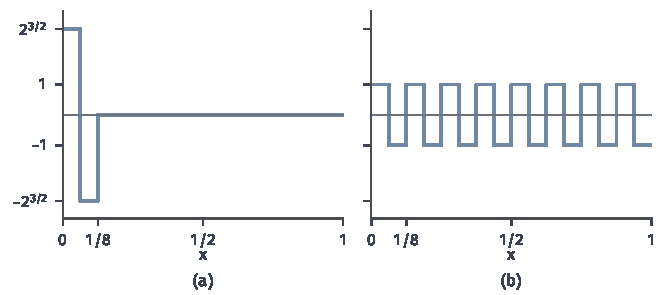
\includegraphics[width=112mm]{figures/04-spaces-measures-and-geometry/03-function-spaces/matplotlib/besov-lp-position/figure.pdf}
  \caption{第$3$层Haar组合。(a)系数集中：$g^{\mathrm A}=\psi_{3,0}$，是一个高$2^{3/2}$、宽$1/8$的脉冲。(b)系数分散：$g^{\mathrm B}=8^{-1/2}\sum_k\psi_{3,k}$，处处$\lvert g^{\mathrm B}\rvert=1$。两者系数的$\ell^2$范数相同。}
  \label{fig:besov-lp-position}
\end{BookInlineFigure}

图~\ref{fig:besov-lp-position}解释了这张表。$L^2$看不出区别，$L^\infty$只看峰值，脉冲因此显得大，$L^1$看总面积，脉冲因此显得小。$2^{j(1/2-1/p)}\lVert c_j\rVert_{\ell^p}$正是第$j$层细节在$L^p$中的大小，$\ell^p$范数把差分范数中“同一尺度、不同位置”的汇总搬到了坐标上。

再乘以$2^{js}$，就把这一层的大小与期望量级$2^{-js}$相比较，对应差分范数中的$t^{-s}$。粗项$a$只有$2^{j_0}$个分量，记录最大尺度上的整体大小，对应差分范数中的$\lVert f\rVert_p$；它不能省略，否则常数函数会得到零范数。

\subsection{小波等价范数}
\label{sec:besov-wavelet-norm}

把上述加权块大小按$\ell^q$汇总，就得到候选的系数范数。记
\begin{equation}
 b_j=2^{j(s+1/2-1/p)}\lVert c_j\rVert_{\ell^p},\qquad j\geq j_0 ,
 \label{eq:besov-block}
\end{equation}
并令
\begin{equation}
 \lVert f\rVert_{B^s_{p,q}}^{\mathrm w}=\lVert a\rVert_{\ell^p}+\bigl\lVert(b_j)_{j\geq j_0}\bigr\rVert_{\ell^q},
 \label{eq:besov-wavelet-norm}
\end{equation}
其中$q=\infty$时取上确界。

图~\ref{fig:besov-group-coordinates}是这个范数的计算过程。它与有限维的分组范数只有两点不同：组数无穷，组的长度$2^j$随下标增长。权重中的$s$体现光滑性要求，$1/2-1/p$只是归一化换算。

\begin{BookInlineFigure}
  \centering
  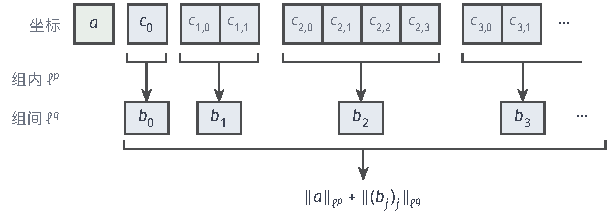
\includegraphics[width=103.3mm]{figures/04-spaces-measures-and-geometry/03-function-spaces/tikz/besov-group-coordinates/figure.pdf}
  \caption{Besov范数是分组加权的向量范数（图中取$j_0=0$）。第一行是函数的小波坐标，蓝色方格按尺度分组，第$j$组有$2^j$个分量，绿色方格是粗项。第二行把每组用$\ell^p$范数合成一个数，并乘以权重，得到式~\eqref{eq:besov-block}的$b_j$。最后对各组的$b_j$取$\ell^q$范数，再加上粗项。}
  \label{fig:besov-group-coordinates}
\end{BookInlineFigure}

用贯穿的例子算一次。取$p=2$、$q=2$、$s=1/4$，此时权重为$2^{j/4}$，每组只有一个非零坐标，所以
\[
 b_j=2^{j/4}\cdot\frac{2^{-j/2}}{3}=\frac{2^{-j/4}}{3}.
\]
前几项约为$0.333$、$0.280$、$0.236$、$0.198$。

对$b_j^2$求几何和，再加上粗项，得到
\[
 \lVert(b_j)\rVert_{\ell^2}^2=\frac{1/9}{1-2^{-1/2}}\approx0.3794,\qquad\lVert f\rVert^{\mathrm w}_{B^{1/4}_{2,2}}=\frac13+\sqrt{0.3794}\approx0.949 .
\]
若取$s=1/2$，则$b_j=1/3$对所有$j$成立，序列有界而不可和，与差分计算得到的式~\eqref{eq:besov-step-membership}一致。

\begin{theorem}[小波刻画]
\label{thm:besov-wavelet-characterization}
设$1\leq p,q\leq\infty$，$s>0$。设$\varphi$与$\psi$有直到$m$阶的连续导数且$m>s$，$\psi$有$M>s$个消失矩，即$\int x^i\psi(x)\,\mathrm dx=0$对$0\leq i<M$成立，$m$与$M$为整数。则存在常数$C_0\geq1$，使对每个$f\in L^p(\mathbb T)$，
\begin{equation}
 C_0^{-1}\lVert f\rVert_{B^s_{p,q}}^{\mathrm w}\leq\lVert f\rVert_{B^s_{p,q}}\leq C_0\lVert f\rVert_{B^s_{p,q}}^{\mathrm w},
 \label{eq:besov-wavelet-equivalence}
\end{equation}
两端同时有限或同时无限。$C_0$依赖$s,p,q$、所选小波与$j_0$。
\end{theorem}

下面写出证明的主要步骤，并分开说明两个方向分别依赖小波的哪种性质。证明中有三处引用外部事实：差分范数不依赖$r$，一般$r$的局部多项式逼近估计，以及$p<2$时小波展开在$L^p$中的收敛。取$r=\lfloor s\rfloor+1$，由$m,M$是大于$s$的整数，得到$s<r\leq\min(m,M)$。记
\[
 g_j=\sum_kc_{j,k}\psi_{j,k},\quad B_j=2^{j(1/2-1/p)}\lVert c_j\rVert_{\ell^p},\quad b_j=2^{js}B_j .
\]

\paragraph{由系数控制差分：正则性}
设系数范数有限。由引理~\ref{lem:besov-single-level}，$\lVert g_j\rVert_p\leq CB_j=C2^{-js}b_j$，而$(b_j)$有界，所以$\sum_jg_j$在$L^p$中绝对收敛，它的系数就是$f$的系数。系数全为零的$L^p$函数只有零：$p\geq2$时这是$L^2$基的完备性，$p<2$时需要用尺度函数核的估计说明投影$P_J$在$L^p$上一致有界。于是$f$等于这个级数。

对单层作差分。小步长用导数，大步长用$2^r$。$g_j^{(r)}$是由$2^{jr}(\psi^{(r)})_{j,k}$组合成的，由引理证明的上界部分，有$\lVert g_j^{(r)}\rVert_p\leq C2^{jr}B_j$。代入式~\eqref{eq:besov-difference-bounds}，得到
\[
 \lVert\Delta_h^rg_j\rVert_p\leq C\min\bigl(1,(2^j\lvert h\rvert)^r\bigr)B_j .
\]

粗项同理，只是因子$2^{jr}$换成常数。对$\lvert h\rvert\leq2^{-J}$求和，把$j<J$与$j\geq J$分开：
\[
 \omega_r(f,2^{-J})_p\leq C\Bigl(2^{-Jr}\lVert a\rVert_{\ell^p}+\sum_{j<J}2^{(j-J)r}B_j+\sum_{j\geq J}B_j\Bigr).
\]

两边乘以$2^{Js}$。用$B_j=2^{-js}b_j$改写，得到
\[
 \begin{aligned}
 2^{Js}\omega_r(f,2^{-J})_p\leq C\Bigl(&2^{-J(r-s)}\lVert a\rVert_{\ell^p}\\
 &+\sum_{j<J}2^{-(J-j)(r-s)}b_j+\sum_{j\geq J}2^{-(j-J)s}b_j\Bigr).
 \end{aligned}
\]

右端是序列$(b_j)$与一个几何衰减序列的卷积。对卷积用$\ell^q$的Minkowski不等式：若$e_J\leq\sum_n\kappa_nb_{J+n}$，$\kappa_n\geq0$，则
\begin{equation}
 \lVert(e_J)\rVert_{\ell^q}\leq\Bigl(\sum_n\kappa_n\Bigr)\lVert(b_j)\rVert_{\ell^q}.
 \label{eq:besov-convolution}
\end{equation}

这里两侧的几何比是$2^{-(r-s)}$和$2^{-s}$，两者都小于$1$，恰好需要$0<s<r$。所以序列$(2^{Js}\omega_r(f,2^{-J})_p)_{J\geq j_0}$的$\ell^q$范数不超过$C(\lVert a\rVert_{\ell^p}+\lVert(b_j)\rVert_{\ell^q})$。$J<j_0$只有有限项，每项不超过$2^r\lVert f\rVert_p$。再代入式~\eqref{eq:besov-dyadic-form}，就得到式~\eqref{eq:besov-wavelet-equivalence}的右半部分。

\paragraph{由差分控制系数：消失矩}
设$\lVert f\rVert_{B^s_{p,q}}<\infty$。先写出通用的一步。把$f$看成实轴上的周期函数，由第~\ref{chap:wavelet-transform}章的展开公式，$c_{j,k}=\int_{\mathbb R}f\psi_{j,k}$，积分区域是实轴上的支撑$I_k$，长度$\delta=L2^{-j}$。因此消失矩可以在实轴上使用，无需担心跨周期接缝。

对次数小于$r\leq M$的多项式$P_k$，有$\int P_k\psi_{j,k}=0$。于是
\[
 c_{j,k}=\int_{I_k}(f-P_k)\psi_{j,k} .
\]
用Hölder不等式与式~\eqref{eq:besov-psi-lp}，再按$k$求和，得到
\[
 B_j^p\leq\lVert\psi\rVert_{p'}^p\sum_k\lVert f-P_k\rVert_{L^p(I_k)}^p .
\]

现在要选$P_k$使右端小。$r=1$时，即$0<s<1$，$P_k$取$f$在$I_k$上的平均值。由Jensen不等式，
\[
 \lvert f(x)-P_k\rvert^p\leq\frac1\delta\int_{I_k}\lvert f(x)-f(y)\rvert^p\,\mathrm dy .
\]

对$x\in I_k$积分并换元$y=x+h$，得到
\[
 \lVert f-P_k\rVert_{L^p(I_k)}^p\leq\frac1\delta\int_{\lvert h\rvert\leq\delta}\int_{I_k}\lvert\Delta_hf(x)\rvert^p\,\mathrm dx\,\mathrm dh .
\]
对$k$求和，每点至多被计入$m$次，$\mathrm dh$的积分域长度为$2\delta$，于是
\[
 \sum_k\lVert f-P_k\rVert_{L^p(I_k)}^p\leq2m\,\omega_1(f,\delta)_p^p .
\]

由$\Delta_{nh}u=\sum_{i<n}\Delta_hu(\cdot+ih)$，得到$\omega_1(f,nt)_p\leq n\,\omega_1(f,t)_p$，所以$B_j\leq C\omega_1(f,2^{-j})_p$。乘以$2^{js}$，取$\ell^q$，由式~\eqref{eq:besov-dyadic-form}，第二项受$\lVert f\rVert_{B^s_{p,q}}$控制。粗项由同样的Hölder估计得到$\lVert a\rVert_{\ell^p}\leq C\lVert f\rVert_p$。这就完成了$0<s<1$时的左半部分。$p=\infty$时把积分换成上确界，论证相同。

$r\geq2$时机制相同，平均值换成局部的最佳多项式逼近，所需的不等式是Whitney估计，它用$r$阶差分在$I_k$附近的平均控制局部多项式逼近误差，证明较长，读者可查阅逼近论的专著。没有足够的消失矩，光滑函数在细尺度上的系数就不会足够小。

\paragraph{条件不能省略}
Haar小波给出具体的反例。Haar母小波是阶跃型函数，由式~\eqref{eq:besov-step-membership}（平移与伸缩只改变常数），它在$p=2$、$s>1/2$时不属于任何$B^s_{2,q}$，在$s=1/2$时只属于$B^{1/2}_{2,\infty}$。可是在式~\eqref{eq:besov-wavelet-norm}中，单个Haar小波只有一个非零系数，系数范数有限。所以对这些参数，Haar系数范数与差分范数不可能等价。

Haar小波在$p=2$、$0<s<1/2$时仍然适用。消失矩的方向只用$r=1$，上面的证明不变。正则性的方向要改一步：第$j$层的Haar组合是网格宽度$2^{-j-1}$上的阶梯函数，$\lVert\Delta_hg_j\rVert_2$只有$(2^j\lvert h\rvert)^{1/2}$的增益，卷积的几何比变成$2^{-(1/2-s)}$，这要求$s<1/2$。这也是本章手算例子可以用Haar基的依据，手算的结果只用于$s<1/2$时的等价，$s=1/2$的端点由式~\eqref{eq:besov-step-membership}另行验证。要刻画更高的光滑阶数，必须改用更光滑、消失矩更多的小波。

下面三节固定一个满足定理~\ref{thm:besov-wavelet-characterization}条件的周期正交小波基，把差分范数与系数范数视为可以互换的度量，相差的倍数统一记入常数$C_0$。

\section{按尺度截断的误差}
\label{sec:besov-scale-truncation}

小波坐标中最直接的近似方法，是对每个函数保留同一个尺度范围内的全部系数，舍去更细的层。本节固定$p=2$，以$L^2$范数度量误差，先写出截断误差的精确公式，再对Besov球给出不依赖函数的统一截断界。最后反过来说明，各个截断尺度上的误差汇总在一起，恰好刻画Besov条件，这也解释了参数$q$在逼近问题中的意义。

$p=2$时，式\eqref{eq:besov-wavelet-norm}的权重化为$2^{js}$，于是由定理~\ref{thm:besov-wavelet-characterization}，
\begin{equation}
C_0^{-1}\Bigl(\lVert a\rVert_{\ell^2}+\bigl\lVert(2^{js}\lVert c_j\rVert_{\ell^2})_{j\geq j_0}\bigr\rVert_{\ell^q}\Bigr)\leq\lVert f\rVert_{B^s_{2,q}}\leq C_0\Bigl(\lVert a\rVert_{\ell^2}+\bigl\lVert(2^{js}\lVert c_j\rVert_{\ell^2})_{j\geq j_0}\bigr\rVert_{\ell^q}\Bigr).
\label{eq:besov-wavelet-norm-l2}
\end{equation}
本节与后面两节都使用这一形式。

\subsection{尺度截断}
\label{sec:besov-truncation}

对整数$J\geq j_0$，令$V_J$为粗项基函数与$j_0\leq j<J$的全部细节小波张成的子空间，$P_J$为到$V_J$的正交投影：
\[
P_Jf=\sum_{k}a_k\varphi_{j_0,k}+\sum_{j_0\leq j<J}\sum_kc_{j,k}\psi_{j,k} .
\]
$V_J$的维数为$M_J=2^{j_0}+\sum_{j=j_0}^{J-1}2^j=2^J$。由正交性与Parseval等式，截断误差
\begin{equation}
E_J(f)=\lVert f-P_Jf\rVert_2,\qquad E_J(f)^2=\sum_{j\geq J}\lVert c_j\rVert_{\ell^2}^2 .
\label{eq:besov-truncation-error}
\end{equation}
由第~\ref{chap:inner-product-spaces}章，$P_Jf$是$V_J$中离$f$最近的元素，所以$E_J(f)$也是在$V_J$中能达到的最佳误差。

这里有两个不同的量需要分开：尺度$J$规定保留到多细的层，项数预算$M_J$规定用了多少个基函数。二者由$M_J=2^J$联系起来，但含义不同，下一节的最佳$N$项逼近只限制项数而不限制尺度。更重要的是，$V_J$在看到任何函数之前就已经选定，对整类函数都相同。这正是第~\ref{chap:function-approximation}章所说的固定子空间逼近：近似是线性的，所有函数共用同一份基函数表。

\subsection{统一截断误差}
\label{sec:besov-uniform-truncation}

现在对Besov球中的所有函数同时估计截断误差。

\begin{theorem}[Besov球上的统一截断界]
\label{thm:besov-uniform-truncation}
设$s>0$，$1\leq q\leq\infty$。存在只依赖$s$与$C_0$的常数$C_s$，使对每个满足$\lVert f\rVert_{B^s_{2,q}}\leq R$的$f$和每个$J\geq j_0$，
\[
E_J(f)\leq C_sR\,2^{-Js}=C_sR\,M_J^{-s} .
\]
\end{theorem}

\begin{proof}
由式\eqref{eq:besov-wavelet-norm-l2}，$\ell^q$范数不小于各项的最大值，所以对每个$j\geq j_0$，$2^{js}\lVert c_j\rVert_{\ell^2}\leq C_0R$，即$\lVert c_j\rVert_{\ell^2}\leq C_0R2^{-js}$。代入式\eqref{eq:besov-truncation-error}，对几何级数求和，
\[
E_J(f)^2\leq C_0^2R^2\sum_{j\geq J}2^{-2js}=\frac{C_0^2R^2\,2^{-2Js}}{1-2^{-2s}} .
\]
取$C_s=C_0(1-2^{-2s})^{-1/2}$，再用$2^J=M_J$即得。
\end{proof}

常数$C_s$不随函数和截断尺度改变，所以这是整类函数的最坏误差界：用$M$个预先固定的基函数，Besov球中每个函数的误差都不超过$C_sRM^{-s}$。这个量级对整类函数不能再改进。取$f=(R/C_0)2^{-Js}\psi_{J,0}$，它的系数范数为$R/C_0$，所以$\lVert f\rVert_{B^s_{2,q}}\leq R$；而它的全部能量都在第$J$层，$E_J(f)=(R/C_0)2^{-Js}$，与上界只差常数倍。注意这个界只用到每层的统一上界，与$q$无关：$q$越大球越大，但每层的最大可能大小相同。

\subsection{截断误差的尺度汇总}
\label{sec:besov-truncation-aggregation}

统一截断界是从Besov条件推出误差。反过来，一个函数在各个截断尺度上的误差，能否读出它属于哪个Besov空间？答案是肯定的，但要把各尺度的误差汇总起来，而不是只看一个速率。

\begin{theorem}[截断误差刻画Besov条件]
\label{thm:besov-truncation-characterization}
设$s>0$，$1\leq q\leq\infty$。存在常数$C$，使对每个$f\in L^2(\mathbb T)$，
\[
C^{-1}\lVert f\rVert_{B^s_{2,q}}\leq\lVert f\rVert_2+\bigl\lVert(2^{Js}E_J(f))_{J\geq j_0}\bigr\rVert_{\ell^q}\leq C\lVert f\rVert_{B^s_{2,q}} ,
\]
两端同时有限或同时无限。
\end{theorem}

\begin{proof}
记$b_j=2^{js}\lVert c_j\rVert_{\ell^2}$，$e_J=2^{Js}E_J(f)$。一个方向来自误差至少包含当前层：由式\eqref{eq:besov-truncation-error}，$\lVert c_J\rVert_{\ell^2}\leq E_J(f)$，所以$b_J\leq e_J$对每个$J$成立。

另一方向来自尾和。平方和的平方根不超过和，所以$E_J(f)\leq\sum_{j\geq J}\lVert c_j\rVert_{\ell^2}$，乘以$2^{Js}$得
\[
e_J\leq\sum_{m\geq0}2^{-ms}b_{J+m} .
\]
对序列$(e_J)_J$取$\ell^q$范数，由Minkowski不等式，右端每个$m$的贡献不超过$2^{-ms}\lVert(b_j)\rVert_{\ell^q}$，于是$\lVert(e_J)\rVert_{\ell^q}\leq(1-2^{-s})^{-1}\lVert(b_j)\rVert_{\ell^q}$。

最后处理粗项：$\lVert a\rVert_{\ell^2}\leq\lVert f\rVert_2$，并且$\lVert f\rVert_2\leq\lVert a\rVert_{\ell^2}+E_{j_0}(f)\leq\lVert a\rVert_{\ell^2}+2^{-j_0s}e_{j_0}$。结合式\eqref{eq:besov-wavelet-norm-l2}即得两侧估计。
\end{proof}

所以$B^s_{2,q}$中的$q$在逼近语言中有直接含义：它规定截断误差序列$(2^{Js}E_J(f))_J$怎样汇总。$q=\infty$要求统一速率$E_J(f)\leq C2^{-Js}$，有限的$q$还要求这些按速率放大的误差跨尺度$q$次可和。

\begin{example}[统一速率与跨尺度可和性]
\label{ex:besov-one-coefficient-per-scale}
令$f=\sum_{j\geq j_0}2^{-js}\psi_{j,0}$，即每层只有一个大小为$2^{-js}$的系数。系数平方可和，$f\in L^2(\mathbb T)$。这时$b_j=1$对每个$j$成立，序列$(b_j)$有界而不$q$次可和；由式\eqref{eq:besov-wavelet-norm-l2}，$f\in B^s_{2,\infty}$，但对任何有限$q$，$f\notin B^s_{2,q}$。截断误差为
\[
E_J(f)=\Bigl(\sum_{j\geq J}2^{-2js}\Bigr)^{1/2}=\frac{2^{-Js}}{(1-2^{-2s})^{1/2}},
\]
恰好具有统一速率$2^{-Js}$。所以仅凭统一衰减速率，只能保证$q=\infty$的条件；有限$q$所需的跨尺度可和性，需要误差在越来越细的尺度上比$2^{-Js}$衰减得更快，并且快到可以$q$次求和。这与第~\ref{sec:besov-distribution-aggregation}小节$b_j=1$与$b_j=1/j$的对比是同一件事。
\end{example}


\section{最佳\texorpdfstring{$N$}{N}项逼近的误差}
\label{sec:besov-best-n-term}

上一节的截断对所有函数保留同一组坐标。若函数的大分量集中在少数几个位置，例如只在跳跃点附近有大的细尺度系数，预先固定的子空间就会把预算花在许多为零的分量上。本节保持同一周期正交小波基和$L^2$误差，改为允许每个函数跨组挑选至多$N$个分量。由第~\ref{chap:function-approximation}章的最大系数选择定理，最优的选择是保留绝对值最大的$N$个分量。

把粗项系数与全部细节系数排成一个序列，记它们的绝对值的非增重排为$c_1^*\geq c_2^*\geq\cdots$。由同一定理，最佳$N$项误差为
\begin{equation}
 \sigma_N(f)_2=\Bigl(\sum_{n>N}(c_n^*)^2\Bigr)^{1/2},
 \label{eq:besov-n-term-error}
\end{equation}
约定$\sigma_0(f)_2=\lVert f\rVert_2$。

为研究系数的集中程度怎样影响这个误差，本节取$0<s<1/2$，令
\begin{equation}
 \frac1\tau=s+\frac12,
 \label{eq:besov-tau}
\end{equation}
从而$1<\tau<2$，并研究$B^s_{\tau,\tau}$的系数条件。本节的函数都取自$L^2(\mathbb T)$，以便讨论$L^2$误差。

\subsection{跨尺度选择}
\label{sec:besov-adaptive-selection}

先看最极端的情形。取$f=\psi_{J',0}$，只有第$J'$组的一个分量非零。固定尺度截断在$J\leq J'$时还没有到达这一组，$E_J(f)=1$，遗漏全部能量，尽管已经用了$M_J=2^J$个基函数。最佳$N$项逼近在$N=1$时就保留这个分量，$\sigma_1(f)_2=0$。

贯穿的例子$f=\mathbf 1_{[0,1/3)}$更有代表性。它的坐标是$a_0=1/3$与每组一个的$2^{-j/2}/3$。按大小排列，$a_0$与第$0$组并列最大，之后是第$1,2,\ldots$组，于是前$N$项保留了$a_0$与第$0$组到第$N-2$组的非零分量。代入式~\eqref{eq:besov-n-term-error}，得到
\[
 \sigma_N(f)_2^2=\sum_{j\geq N-1}\frac{2^{-j}}{9}=\frac{2^{2-N}}{9},\qquad\sigma_N(f)_2=\frac23\,2^{-N/2}.
\]

$N$也取$8$，得到$\sigma_8(f)_2=1/24\approx0.0417$，是上一节$E_3(f)=1/6$的四分之一。图~\ref{fig:besov-haar-tiles}比较这两种选择：一个方格代表一个分量，上方的行是粗尺度。固定截断把$8$项用在前三层的全部方格上，其中一半的系数为零；最佳$N$项沿着跳跃点一路向下，每层只取一个方格。

\begin{BookInlineFigure}
  \centering
  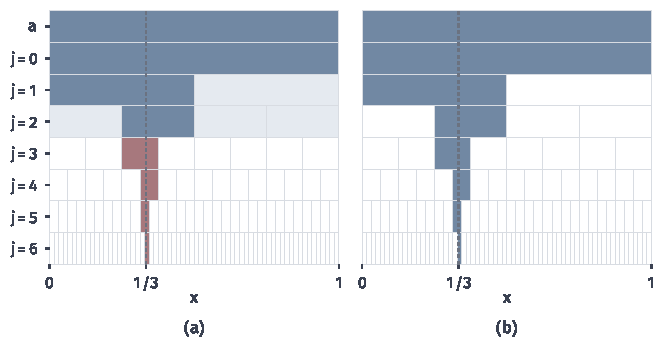
\includegraphics[width=112mm]{figures/04-spaces-measures-and-geometry/03-function-spaces/matplotlib/besov-haar-tiles/figure.pdf}
  \caption{$f=\mathbf 1_{[0,1/3)}$的Haar坐标，每个方格是一个基函数的位置和尺度，虚线标出跳跃点$x=1/3$。每层只有含跳跃点的方格系数非零。(a)固定尺度截断：浅蓝色是保留而系数为零的项，深蓝色是保留的非零项，红色是舍弃的非零项。(b)最佳$N$项：$N=8$项全部用在非零系数上。}
  \label{fig:besov-haar-tiles}
\end{BookInlineFigure}

两种做法的误差差别如表~\ref{tab:besov-fixed-vs-best}，图~\ref{fig:besov-error-decay}画出同样的数据。固定截断的误差按项数的$-1/2$次幂下降，最佳$N$项的误差按项数指数下降。

\begin{BookInlineTable}
  \centering
  \begin{tabular}{@{}cccccc@{}}
    \toprule
    项数 & $1$ & $2$ & $4$ & $8$ & $16$\\
    \midrule
    固定截断$E_J$（$M=2^J$） & $0.471$ & $0.333$ & $0.236$ & $0.167$ & $0.118$\\
    最佳$N$项$\sigma_N$ & $0.471$ & $0.333$ & $0.167$ & $0.042$ & $0.003$\\
    \bottomrule
  \end{tabular}
  \caption{$f=\mathbf 1_{[0,1/3)}$在Haar基下的两种误差。}
  \label{tab:besov-fixed-vs-best}
\end{BookInlineTable}

\begin{BookInlineFigure}
  \centering
  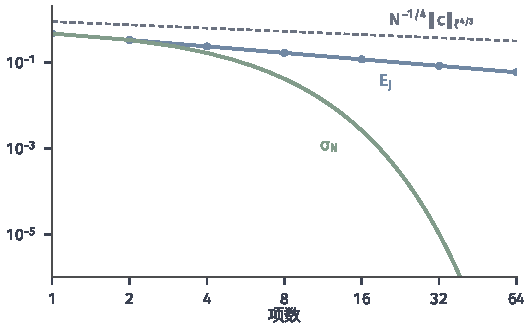
\includegraphics[width=90mm]{figures/04-spaces-measures-and-geometry/03-function-spaces/matplotlib/besov-error-decay/figure.pdf}
  \caption{同一函数的两种误差，双对数坐标。蓝色为固定截断$E_J$，圆点在$M=2^J$处；绿色为最佳$N$项误差$\sigma_N$；灰色虚线是定理~\ref{thm:besov-n-term-upper}在$s=1/4$时给出的上界。}
  \label{fig:besov-error-decay}
\end{BookInlineFigure}

换成更光滑的紧支撑小波，同样的现象仍然出现。设$\int\psi=0$。若$\psi_{j,k}$的支撑内部不含跳跃点，$f$在其上为常数，系数为零；含跳跃点的$k$每层只有有界个，并且
\[
 \lvert c_{j,k}\rvert\leq\lVert\psi_{j,k}\rVert_1=2^{-j/2}\lVert\psi\rVert_1 .
\]
所以每层只有有界个非零系数，大小按$2^{-j/2}$衰减，$\sigma_N$仍随$N$指数衰减。

固定截断则不然。阶跃函数不属于任何$s>1/2$的$B^s_{2,\infty}$，由定理~\ref{thm:besov-truncation-characterization}，$E_J(f)=O(2^{-Js})$对$s>1/2$不成立，用$M$个固定基函数的误差不能比$M^{-1/2}$快出一个幂次。

两种方式的差别在于保留哪些方向：固定截断按下标保留，自适应选择按大小保留。代价有两点。每个函数各自选择$N$个下标，要用有限个代表覆盖整个函数类时，还必须计入“选了哪些下标”这一信息。近似对$f$也不再是线性的：两个函数之和的最佳$N$项近似，一般不是各自近似之和。

\subsection{最佳\texorpdfstring{$N$}{N}项误差的上界}
\label{sec:besov-n-term-upper}

在$1/\tau=s+1/2$时，小波范数~\eqref{eq:besov-wavelet-norm}中$p=q=\tau$，权重$2^{j(s+1/2-1/\tau)}=1$完全抵消。组内和组间都用$\ell^\tau$，分组也就不再起作用：
\[
 \lVert f\rVert_{B^s_{\tau,\tau}}^{\mathrm w}=\lVert a\rVert_{\ell^\tau}+\Bigl(\sum_{j\geq j_0}\lVert c_j\rVert_{\ell^\tau}^\tau\Bigr)^{1/\tau}.
\]

记$c$为全部系数（包括有限个粗项）组成的序列。对非负数$A,B$有下面的比较：
\[
 (A^\tau+B^\tau)^{1/\tau}\leq A+B\leq2(A^\tau+B^\tau)^{1/\tau} .
\]
取$A=\lVert a\rVert_{\ell^\tau}$，$B$为细节部分的$\ell^\tau$范数，得到
\begin{equation}
 \lVert c\rVert_{\ell^\tau}\leq\lVert f\rVert^{\mathrm w}_{B^s_{\tau,\tau}}\leq2\lVert c\rVert_{\ell^\tau}.
 \label{eq:besov-ltau-coeff}
\end{equation}
所以$f\in B^s_{\tau,\tau}$恰好意味着全部系数$\tau$次可和，不再区分它们来自哪一层。

$\tau<2$时，$\ell^\tau$可和比平方可和更强。这与有限维中的现象相同：在单位$\ell^2$球面上，$\ell^\tau$范数小的向量大部分能量集中在少数分量上。表~\ref{tab:besov-concentrate-spread}中，$\tau=1$时集中的$c^{\mathrm A}$范数是$1$，分散的$c^{\mathrm B}$范数是$2^{3/2}$。

\begin{theorem}[最佳$N$项误差的上界]
\label{thm:besov-n-term-upper}
设$0<s<1/2$，$1/\tau=s+1/2$。则对每个$f\in L^2(\mathbb T)\cap B^s_{\tau,\tau}$和每个$N\geq1$，
\begin{equation}
 \sigma_N(f)_2\leq N^{-s}\lVert c\rVert_{\ell^\tau}\leq C_0N^{-s}\lVert f\rVert_{B^s_{\tau,\tau}} .
 \label{eq:besov-n-term-upper}
\end{equation}
\end{theorem}

\begin{proof}
重排序列的前$n$项都不小于$c_n^*$，所以$n(c_n^*)^\tau\leq\lVert c\rVert_{\ell^\tau}^\tau$，即
\[
 c_n^*\leq n^{-1/\tau}\lVert c\rVert_{\ell^\tau} .
\]

把式~\eqref{eq:besov-n-term-error}中每一项写成$(c_n^*)^2=(c_n^*)^{2-\tau}(c_n^*)^\tau$。$n>N$时$c_n^*\leq c_N^*$，于是
\[
 \sigma_N(f)_2^2\leq(c_N^*)^{2-\tau}\sum_{n>N}(c_n^*)^\tau\leq(c_N^*)^{2-\tau}\lVert c\rVert_{\ell^\tau}^\tau .
\]

代入$c_N^*$的上界，并用$(2-\tau)/\tau=2/\tau-1=2s$，得到
\[
 \sigma_N(f)_2^2\leq N^{-(2-\tau)/\tau}\lVert c\rVert_{\ell^\tau}^{2-\tau}\lVert c\rVert_{\ell^\tau}^\tau=N^{-2s}\lVert c\rVert_{\ell^\tau}^2 .
\]
第二个不等式由式~\eqref{eq:besov-ltau-coeff}与定理~\ref{thm:besov-wavelet-characterization}得到。
\end{proof}

用贯穿的例子核对。取$s=1/4$，则$\tau=4/3$。全部系数的$\ell^{4/3}$范数由几何级数给出：
\[
 \lVert c\rVert_{\ell^{4/3}}^{4/3}=3^{-4/3}\Bigl(1+\frac{1}{1-2^{-2/3}}\Bigr)\approx0.8557,\qquad\lVert c\rVert_{\ell^{4/3}}\approx0.890 .
\]
$N=8$时上界为$8^{-1/4}\times0.890\approx0.529$，实际误差$0.0417$远小于它。这个上界对整个球成立，它要照顾到最坏的函数，而这个例子的系数衰减得特别快。

图~\ref{fig:besov-parameter-map}把几个空间放到$(1/p,s)$平面上。竖线$p=2$上的点是上一节的$B^s_{2,q}$，球上的固定截断速率是$M^{-s}$。绿线上的点是$B^s_{\tau,\tau}$，球上的最佳$N$项速率是同样的$N^{-s}$。从竖线沿箭头移到绿线，速率不变，度量方式却换成了$\ell^\tau$：函数可以把大系数集中在少数位置，只要全部系数$\tau$次可和。

\begin{BookInlineFigure}
  \centering
  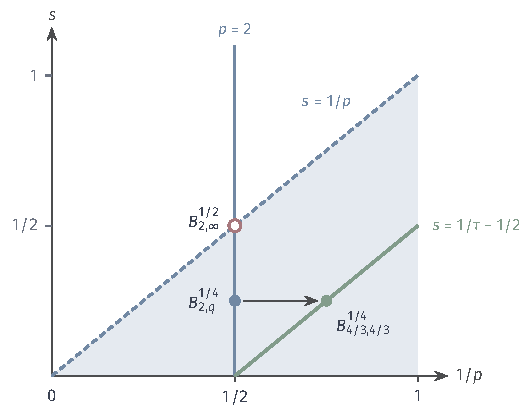
\includegraphics[width=90.1mm]{figures/04-spaces-measures-and-geometry/03-function-spaces/tikz/besov-parameter-map/figure.pdf}
  \caption{$(1/p,s)$平面上的Besov空间。蓝色竖线是$p=2$，绿线是$s=1/\tau-1/2$，箭头两端速率相同。虚线$s=1/p$是周期阶跃的临界线，其下方的浅蓝色区域内阶跃函数属于相应空间，红圈标出竖线上的临界点$B^{1/2}_{2,\infty}$。绿线整条位于浅蓝色区域内。}
  \label{fig:besov-parameter-map}
\end{BookInlineFigure}

图中还能读出阶跃函数为什么适合自适应逼近。在竖线上，阶跃函数的光滑阶数到$1/2$就停了。绿线却整条在临界线以下，因为$s=1/\tau-1/2<1/\tau$。在本节的范围$0<s<1/2$内，阶跃函数属于绿线上的每个空间。

\subsection{速率条件的逆向刻画}
\label{sec:besov-n-term-converse}

上界的反方向是：若误差满足$\sup_NN^s\sigma_N(f)_2<\infty$，函数是否属于$B^s_{\tau,\tau}$？答案是否定的，速率只对应一个更弱的条件。

\begin{theorem}[误差速率的刻画]
\label{thm:besov-n-term-rate}
设$s>0$，$1/\tau=s+1/2$，$f\in L^2(\mathbb T)$。则
\begin{equation}
 \sup_{N\geq1}N^s\sigma_N(f)_2<\infty\iff\sup_{n\geq1}n^{1/\tau}c_n^*<\infty .
 \label{eq:besov-n-term-rate}
\end{equation}
\end{theorem}

\begin{proof}
设$\sigma_N(f)_2\leq AN^{-s}$。第$N+1$到$2N$项共$N$项，都不小于$c_{2N}^*$，所以
\[
 N(c_{2N}^*)^2\leq\sum_{n=N+1}^{2N}(c_n^*)^2\leq\sigma_N(f)_2^2\leq A^2N^{-2s}.
\]
由此得到
\[
 c_{2N}^*\leq AN^{-s-1/2}=AN^{-1/\tau}.
\]
奇数下标用$c_{2N+1}^*\leq c_{2N}^*$，$n=1$用$c_1^*\leq\lVert f\rVert_2$，于是$\sup_nn^{1/\tau}c_n^*<\infty$。

反过来，设$c_n^*\leq Bn^{-1/\tau}$。代入式~\eqref{eq:besov-n-term-error}，用积分比较尾和，并用$2/\tau-1=2s>0$，得到
\[
 \sigma_N(f)_2^2\leq B^2\sum_{n>N}n^{-2/\tau}\leq B^2\int_N^\infty x^{-2/\tau}\,\mathrm dx=\frac{B^2N^{-2s}}{2s}.
\]
\end{proof}

条件$\sup_nn^{1/\tau}c_n^*<\infty$称为弱$\ell^\tau$条件，它比$\ell^\tau$可和弱。取$c_n^*=n^{-1/\tau}$，由$2/\tau=2s+1>1$，它平方可和，按任意次序放到基函数上就得到一个$L^2$函数$f$。它满足弱$\ell^\tau$条件，因而
\[
 \sigma_N(f)_2\leq(2s)^{-1/2}N^{-s}.
\]

可是$\sum_n(c_n^*)^\tau=\sum_nn^{-1}=\infty$，所以在$0<s<1/2$时$f\notin B^s_{\tau,\tau}$。单一的误差速率不能反推Besov成员资格，这与统一截断速率只对应$q=\infty$的情形相似。

\subsection{跨预算的误差汇总}
\label{sec:besov-approximation-spaces}

第~\ref{sec:besov-truncation-aggregation}小节看到，把截断误差跨尺度汇总可以恢复有限$q$的条件。对最佳$N$项误差也可以这样做：不只要求一个速率，而是把各个预算下的误差按$\ell^\tau$汇总。预算取二进值$N=2^m$。

\begin{definition}[逼近空间]
\label{def:besov-approximation-space}
设$s>0$，$1/\tau=s+1/2$。对$f\in L^2(\mathbb T)$，令
\begin{equation}
 \lVert f\rVert_{A^s_\tau}=\lVert f\rVert_2+\Bigl(\sum_{m\geq0}\bigl(2^{ms}\sigma_{2^m}(f)_2\bigr)^\tau\Bigr)^{1/\tau},
 \label{eq:besov-approximation-space}
\end{equation}
使其有限的函数组成的集合称为\term{逼近空间}（approximation space），记为$A^s_\tau$。
\end{definition}

$\sigma_N$随$N$单调不增，二进预算之间只差常数倍，所以$\sup_m2^{ms}\sigma_{2^m}(f)_2<\infty$等价于$\sup_NN^s\sigma_N(f)_2<\infty$。把上确界换成$\ell^\tau$和，正是把“统一速率”加强为“误差汇总”。

\begin{theorem}[逼近空间与Besov空间]
\label{thm:besov-approximation-equals-besov}
设$0<s<1/2$，$1/\tau=s+1/2$，小波满足定理~\ref{thm:besov-wavelet-characterization}的条件。则对$f\in L^2(\mathbb T)$，$f\in A^s_\tau$当且仅当$f\in B^s_{\tau,\tau}$，并且两个范数等价。
\end{theorem}

\begin{proof}
由式~\eqref{eq:besov-ltau-coeff}和定理~\ref{thm:besov-wavelet-characterization}，$\lVert f\rVert_{B^s_{\tau,\tau}}$与$\lVert c\rVert_{\ell^\tau}$等价，所以只需比较$\lVert f\rVert_{A^s_\tau}$与$\lVert c\rVert_{\ell^\tau}$。

先由系数控制误差汇总。由Parseval等式和$\tau<2$，$\lVert f\rVert_2$不超过$\lVert c\rVert_{\ell^\tau}$。把下标按二进块$2^l<n\leq2^{l+1}$分组，每块有$2^l$项，每项不超过$c_{2^l}^*$，所以
\[
 \sigma_{2^m}(f)_2^2\leq\sum_{l\geq m}2^l(c_{2^l}^*)^2 .
\]

记$\beta_l=2^{l/\tau}c_{2^l}^*$，则$2^l(c_{2^l}^*)^2=2^{-2ls}\beta_l^2$。乘以$2^{2ms}$并开方，得到
\[
 2^{ms}\sigma_{2^m}(f)_2\leq\Bigl(\sum_{l\geq m}2^{-2(l-m)s}\beta_l^2\Bigr)^{1/2}\leq\sum_{l\geq m}2^{-(l-m)s}\beta_l .
\]
由式~\eqref{eq:besov-convolution}，左端序列的$\ell^\tau$范数不超过$(1-2^{-s})^{-1}\lVert(\beta_l)\rVert_{\ell^\tau}$。

余下要用$\lVert c\rVert_{\ell^\tau}$控制$\lVert(\beta_l)\rVert_{\ell^\tau}$。$l\geq1$时，第$2^{l-1}+1$到$2^l$项共$2^{l-1}$项，都不小于$c_{2^l}^*$，所以
\[
 2^{l-1}(c_{2^l}^*)^\tau\leq\sum_{2^{l-1}<n\leq2^l}(c_n^*)^\tau .
\]
对$l$求和，并单独计入$\beta_0=c_1^*$，得到
\[
 \sum_{l\geq0}\beta_l^\tau\leq2\lVert c\rVert_{\ell^\tau}^\tau .
\]

再由误差汇总控制系数。下标$2^{m+1}\leq n<2^{m+2}$的块有$2^{m+1}$项，每项不超过$c_{2^{m+1}}^*$。由上一小节的论证，$2^m(c_{2^{m+1}}^*)^2\leq\sigma_{2^m}(f)_2^2$。所以
\[
 \begin{aligned}
 \sum_{n\geq2}(c_n^*)^\tau&\leq\sum_{m\geq0}2^{m+1}(c_{2^{m+1}}^*)^\tau\\
 &\leq2\sum_{m\geq0}2^{m(1-\tau/2)}\sigma_{2^m}(f)_2^\tau\\
 &=2\sum_{m\geq0}\bigl(2^{ms}\sigma_{2^m}(f)_2\bigr)^\tau ,
 \end{aligned}
\]
最后一步用了$\tau s=1-\tau/2$，它等价于$1/\tau=s+1/2$。

加上$c_1^*\leq\lVert f\rVert_2$，得到
\[
 \lVert c\rVert_{\ell^\tau}^\tau\leq\lVert f\rVert_2^\tau+2\lVert f\rVert_{A^s_\tau}^\tau .
\]
\end{proof}

这个定理说明，比统一速率更强的误差汇总恰好恢复了系数的强可和性。它依赖本节固定的条件：同一正交小波基，$L^2$误差，$1/\tau=s+1/2$，以及满足小波刻画条件的小波。换成冗余字典、其他误差范数或不匹配的指数，都需要另行分析。

\section{Besov球的覆盖数}
\label{sec:besov-covering}

前两节回答的是“给一个函数，用多少项能达到给定误差”。另一类问题是：为整类函数预先准备有限个代表，使类中每个函数都离某个代表足够近，至少需要多少个代表？第~\ref{chap:sobolev-spaces}章的紧嵌入只说明Sobolev球的覆盖数有限，没有给出增长阶。本节回到第~\ref{sec:besov-scale-truncation}节的$B^s_{2,q}$有界类，在$L^2$距离下算出覆盖数随精度的增长：固定尺度截断控制尾部，逐尺度覆盖保留的系数给出上界，再用只在单一尺度上变化的子类给出同阶的下界。

\subsection{函数类、距离与精度}
\label{sec:besov-cover-setting}

固定单位周期、$s>0$、$1\leq q\leq\infty$与$R>0$，令
\[
\mathcal F_R=\{f\in L^2(\mathbb T):\lVert f\rVert_{B^s_{2,q}}\leq R\}.
\]
沿用第~\ref{chap:metric-spaces}章的覆盖数：记$N(\varepsilon,\mathcal F_R)$为覆盖$\mathcal F_R$所需的半径为$\varepsilon$的$L^2$闭球的最少个数，球心可以取在整个$L^2(\mathbb T)$中。若要求球心属于$\mathcal F_R$，由那里的比较$N_X(\varepsilon,A)\leq N_A(\varepsilon,A)\leq N_X(\varepsilon/2,A)$，只需把半径调整一个固定的因子，下面的增长阶不变。

我们关心$\varepsilon\to0$时$\log N(\varepsilon,\mathcal F_R)$怎样增长，即度量熵。$\mathcal F_R$在$L^2$中全有界：统一截断界说明它离有限维子空间$V_J$一致地近，而它在$V_J$上的投影是有界集。下面把这个定性论证做成定量计数。

\subsection{逐尺度精度分配}
\label{sec:besov-precision-allocation}

由第~\ref{sec:besov-uniform-truncation}小节，类中每个函数满足$E_J(f)\leq C_sR2^{-Js}$，并且由式\eqref{eq:besov-wavelet-norm-l2}，每层系数满足$\lVert a\rVert_{\ell^2}\leq C_0R$，$\lVert c_j\rVert_{\ell^2}\leq C_0R2^{-js}$。覆盖的构造分两部分：尾部直接舍去，保留的系数逐层覆盖。

\emph{尾部。}设$0<\varepsilon<2C_sR\,2^{-(j_0+1)s}$，取$J$为使$C_sR2^{-Js}\leq\varepsilon/2$的最小整数。这一假设保证$J>j_0+1$，并且由最小性$C_sR2^{-(J-1)s}>\varepsilon/2$。于是每个函数的尾部误差$E_J(f)\leq\varepsilon/2$，并且
\begin{equation}
\frac{R}{\varepsilon}\leq\frac{2^{Js}}{2C_s},\qquad2^J<2\Bigl(\frac{2C_sR}{\varepsilon}\Bigr)^{1/s}.
\label{eq:besov-cover-scale}
\end{equation}

\emph{保留的系数。}把粗项$a$并入起始一层，组成维数为$2^{j_0}+2^{j_0}=2^{j_0+1}$的块$(a,c_{j_0})$，半径至多$\sqrt2C_0R$；其余每个$j_0<j<J$的块$c_j$维数为$2^j$，半径至多$C_0R2^{-js}$。对第$j$块分配覆盖精度
\[
\delta_j=\frac\varepsilon2\,2^{-(J-j)/2},\qquad j_0\leq j<J .
\]
越粗的层分到越大的精度，因为它们半径大而维数小；越接近截断尺度的层精度越细。总和满足
\[
\sum_{j_0\leq j<J}\delta_j^2=\frac{\varepsilon^2}{4}\sum_{j_0\leq j<J}2^{-(J-j)}<\frac{\varepsilon^2}{4}\sum_{m\geq1}2^{-m}=\frac{\varepsilon^2}4 .
\]

\emph{合并。}对每块取一个$\delta_j$覆盖，从每块的覆盖中各选一个中心，组成$V_J$中的一个函数$g$。给定$f\in\mathcal F_R$，在每块中选取与$f$的该块系数相距不超过$\delta_j$的中心。由正交性，误差的平方等于各块误差平方与尾部误差平方之和：
\[
\lVert f-g\rVert_2^2\leq\sum_{j_0\leq j<J}\delta_j^2+E_J(f)^2<\frac{\varepsilon^2}4+\frac{\varepsilon^2}4<\varepsilon^2 .
\]
所以这些组合中心构成$\mathcal F_R$的$\varepsilon$覆盖，个数是各块覆盖个数的乘积。

\subsection{对数覆盖数的上界}
\label{sec:besov-entropy-upper}

现在计数。每块通过正交坐标等距地对应于欧氏空间中的球。由第~\ref{chap:metric-spaces}章，$n$维实赋范空间中半径为$\rho$的闭球可以用不超过$(1+2\rho/\delta)^n$个半径为$\delta$的闭球覆盖。

\begin{theorem}[对数覆盖数的上界]
\label{thm:besov-entropy-upper}
设$s>0$，$1\leq q\leq\infty$。存在只依赖$s,q$与所选小波的常数$c,C>0$，使对$0<\varepsilon\leq cR$，
\[
\log N(\varepsilon,\mathcal F_R)\leq C\Bigl(\frac R\varepsilon\Bigr)^{1/s}.
\]
\end{theorem}

\begin{proof}
取$c=C_s2^{-(j_0+1)s}$，则$\varepsilon\leq cR$保证上一小节的假设成立。记$\rho_j$为第$j$块的半径。对$j_0<j<J$，由式\eqref{eq:besov-cover-scale}与$C_0\leq C_s$，
\[
\frac{2\rho_j}{\delta_j}\leq\frac{4C_0R\,2^{-js}2^{(J-j)/2}}{\varepsilon}\leq\frac{2C_0}{C_s}2^{(J-j)s}2^{(J-j)/2}\leq2\cdot2^{(J-j)(s+1/2)},
\]
所以$\log(1+2\rho_j/\delta_j)\leq\log3+(J-j)(s+1/2)\log2\leq C_1(1+J-j)$。起始块的半径多一个因子$\sqrt2\,2^{j_0s}$，只改变常数。按块相乘再取对数，
\[
\log N(\varepsilon,\mathcal F_R)\leq\sum_{j_0\leq j<J}2^{j+1}C_1(1+J-j)\leq2C_1\,2^J\sum_{m\geq1}2^{-m}(1+m)=6C_1\,2^J ,
\]
这里令$m=J-j$，并用了$\sum_{m\geq1}2^{-m}=1$与$\sum_{m\geq1}m2^{-m}=2$。再由式\eqref{eq:besov-cover-scale}，$2^J<2(2C_sR/\varepsilon)^{1/s}$，即得结论。
\end{proof}

估计的对象是对数覆盖数，不是覆盖数本身：覆盖数按$\exp(C(R/\varepsilon)^{1/s})$增长。计数的主要部分来自接近截断尺度的几层，那里维数最大；每层贡献“维数乘以$1+J-j$”，几何权重使总和与最细保留层的维数$2^J$同阶。常数依赖固定的$s,q$与小波，适用范围是$0<\varepsilon\leq cR$；$\varepsilon$与$R$同阶或更大时，少数几个代表就够了。

\subsection{覆盖数的下界}
\label{sec:besov-entropy-lower}

上界是否太粗？我们用一个只在单一尺度上变化的子类核对。

\begin{theorem}[对数覆盖数的下界]
\label{thm:besov-entropy-lower}
在定理~\ref{thm:besov-entropy-upper}的条件下，存在常数$c',c''>0$，使对$0<\varepsilon\leq c''R$，
\[
\log N(\varepsilon,\mathcal F_R)\geq c'\Bigl(\frac R\varepsilon\Bigr)^{1/s}.
\]
\end{theorem}

\begin{proof}
令$\alpha=1/C_0$。对$j\geq j_0$，考虑只允许第$j$层系数变化、其余系数为零的函数$f=\sum_kx_k\psi_{j,k}$，$\lVert x\rVert_{\ell^2}\leq\alpha R2^{-js}$。它的系数范数为$2^{js}\lVert x\rVert_{\ell^2}\leq\alpha R$，所以$\lVert f\rVert_{B^s_{2,q}}\leq C_0\alpha R=R$，这些函数组成$\mathcal F_R$的子集$\mathcal G_j$。$\mathcal G_j$等距于$2^j$维欧氏空间中半径$\rho=\alpha R2^{-js}$的闭球。

覆盖$\mathcal F_R$的球也覆盖$\mathcal G_j$。到第$j$层子空间的正交投影不增大与该子空间中点的距离，所以可以把球心都投影到这个子空间中。$N$个半径$\varepsilon$的球覆盖半径$\rho$的球，比较体积得$N\varepsilon^{2^j}\geq\rho^{2^j}$，即$\log N\geq2^j\log(\rho/\varepsilon)$。

选择尺度：数列$\alpha R2^{-js}$（$j\geq j_0$）每步缩小因子$2^s$，若$\varepsilon\leq\alpha R2^{-j_0s}/4$，则恰有一个$j$满足$4\varepsilon\leq\alpha R2^{-js}<2^{s+2}\varepsilon$。对这个$j$，$\rho/\varepsilon\geq4$，所以$\log N\geq2^j\log4$；又$2^{js}>\alpha R/(2^{s+2}\varepsilon)$，即$2^j>(\alpha/2^{s+2})^{1/s}(R/\varepsilon)^{1/s}$。合并即得结论，$c'=\log4\cdot(\alpha/2^{s+2})^{1/s}$。
\end{proof}

上下界合起来，$\log N(\varepsilon,\mathcal F_R)$与$(R/\varepsilon)^{1/s}$同阶，增长阶由光滑阶数$s$决定，与汇总指数$q$无关：$q$改变球的大小，但单尺度子类与逐尺度上界只用到每层的统一界，两端的量级相同。这个结论依赖本节固定的设定，即单位周期、$p=2$的Besov球与$L^2$距离；其他积分指数、误差范数或区域需要另行分析，例如目标范数与$p$不同时，单尺度子类不再是欧氏球。与Sobolev紧嵌入只给出“有限”相比，这里的小波坐标把函数类分解为一串维数与半径都已知的有限维球，计数因而可以完成。

\section{与Sobolev空间的联系}
\label{sec:besov-sobolev}

Besov空间是为补充Sobolev条件而引入的，自然要问二者在重合处是否一致。本节只对照第~\ref{chap:sobolev-spaces}章已经定义的一阶平方可积弱导数：在单位周期设定下，$B^1_{2,2}$恰好由端点值相同的$H^1(0,1)$函数组成，范数等价。随后说明端点条件与二阶差分各自为何必要，再用其他参数说明Besov空间在Sobolev空间之外增加了什么。

\paragraph{定理与证明}
记$H^1_{\mathrm{per}}=\{f\in H^1(0,1):\tilde f(0)=\tilde f(1)\}$，其中$\tilde f$是$f$的绝对连续代表，这类函数按周期$1$延拓后在接缝处连续。

\begin{theorem}[$B^1_{2,2}$与周期$H^1$]
\label{thm:besov-b122-h1}
在单位周期上，$B^1_{2,2}(\mathbb T)=H^1_{\mathrm{per}}$，并且存在常数$C$，使$C^{-1}\lVert f\rVert_{H^1(0,1)}\leq\lVert f\rVert_{B^1_{2,2}}\leq C\lVert f\rVert_{H^1(0,1)}$。
\end{theorem}

证明借助周期Fourier系数$\widehat f(k)=\int_0^1f(x)e^{-2\pi\mathrm ikx}\,\mathrm dx$，分两步：先说明$H^1_{\mathrm{per}}$恰好由$\sum_kk^2|\widehat f(k)|^2<\infty$的函数组成，再说明$B^1_{2,2}$的半范数平方与这个和等价。

\emph{第一步：Fourier系数刻画$H^1_{\mathrm{per}}$。}设$f\in H^1_{\mathrm{per}}$。对绝对连续代表分部积分，
\begin{equation*}
\begin{aligned}
\widehat{f'}(k)&=\Bigl[\tilde f(x)e^{-2\pi\mathrm ikx}\Bigr]_0^1+2\pi\mathrm ik\int_0^1\tilde f(x)e^{-2\pi\mathrm ikx}\,\mathrm dx\\
&=\bigl(\tilde f(1)-\tilde f(0)\bigr)+2\pi\mathrm ik\,\widehat f(k)=2\pi\mathrm ik\,\widehat f(k),
\end{aligned}
\end{equation*}
端点条件正好消去边界项。由Parseval等式，$\lVert f'\rVert_2^2=4\pi^2\sum_kk^2|\widehat f(k)|^2<\infty$。反过来，设$\sum_kk^2|\widehat f(k)|^2<\infty$，则$g=\sum_k2\pi\mathrm ik\widehat f(k)e^{2\pi\mathrm ikx}\in L^2$，且$\widehat g(0)=0$。令$F(x)=c+\int_0^xg$，常数$c$使$\int_0^1F=\widehat f(0)$。$F$绝对连续，$F(1)-F(0)=\widehat g(0)=0$；对$k\neq0$分部积分得$\widehat F(k)=\widehat g(k)/(2\pi\mathrm ik)=\widehat f(k)$。Fourier系数全部相同，由完备性$F=f$几乎处处，所以$f\in H^1_{\mathrm{per}}$。

\emph{第二步：半范数与系数和等价。}$s=1$时须取$r\geq2$，这里取$r=2$。由式\eqref{eq:besov-difference-fourier}，$\lVert\Delta_h^2f\rVert_2^2=\sum_k(2|\sin(\pi kh)|)^4|\widehat f(k)|^2$。下界：$\omega_2(f,t)_2\geq\lVert\Delta_t^2f\rVert_2$，交换求和与积分，
\[
|f|_{B^1_{2,2}}^2\geq\sum_k|\widehat f(k)|^2\int_0^1t^{-3}\,16\sin^4(\pi kt)\,\mathrm dt .
\]
对$k\neq0$换元$u=|k|t$，内层积分等于$k^2\int_0^{|k|}16u^{-3}\sin^4(\pi u)\,\mathrm du\geq c_1k^2$，其中$c_1=16\int_0^1u^{-3}\sin^4(\pi u)\,\mathrm du$为正的有限数（被积函数在$u\to0$时约为$\pi^4u$）。上界：$(2|\sin(\pi kh)|)^4\leq\min\bigl(16,(2\pi|k||h|)^4\bigr)$，右端随$|h|$不减，所以$\omega_2(f,t)_2^2\leq\sum_k\min(16,(2\pi|k|t)^4)|\widehat f(k)|^2$；同样换元，$\int_0^1t^{-3}\min(16,(2\pi|k|t)^4)\,\mathrm dt\leq C_1k^2$，$C_1=\int_0^\infty u^{-3}\min(16,(2\pi u)^4)\,\mathrm du<\infty$。于是
\[
c_1\sum_kk^2|\widehat f(k)|^2\leq|f|_{B^1_{2,2}}^2\leq C_1\sum_kk^2|\widehat f(k)|^2 .
\]
两步合并，$f\in B^1_{2,2}$当且仅当$f\in H^1_{\mathrm{per}}$，且$|f|_{B^1_{2,2}}$与$\lVert f'\rVert_2$等价；再加上$\lVert f\rVert_2$，两个范数等价。

\paragraph{端点条件的作用}
不能把全部$H^1(0,1)$当作周期空间。$f(x)=x$属于$H^1(0,1)$，但$\tilde f(0)=0\neq1=\tilde f(1)$，按周期延拓后在每个整数点跳跃。直接计算，$k\neq0$时$\widehat f(k)=-1/(2\pi\mathrm ik)$，于是$k^2|\widehat f(k)|^2=1/(4\pi^2)$不可和，$f\notin B^1_{2,2}$。它的系数与周期阶跃同样按$1/|k|$衰减，周期延拓后的光滑阶数只有$1/2$。第一步的分部积分清楚地显示了原因：边界项$\tilde f(1)-\tilde f(0)$不为零时，$\widehat{f'}(k)$与$2\pi\mathrm ik\widehat f(k)$相差一个常数，这个常数正是接缝处的跳跃。

\paragraph{二阶差分的必要性}
$s=1$时差分阶数必须取$r\geq2$。若用一阶差分，由第~\ref{sec:besov-modulus}小节的饱和现象，任何非常数的$f$都有某个$\widehat f(k)\neq0$，$k\neq0$；当$|k|t\leq1/2$时，$\omega_1(f,t)_2\geq2|\sin(\pi kt)||\widehat f(k)|\geq4|k|t|\widehat f(k)|$，所以$t^{-1}\omega_1(f,t)_2$在小$t$处有正的下界，$\int_0(t^{-1}\omega_1)^2\,\mathrm dt/t$发散。用一阶差分写出的“$B^1_{2,2}$”只含常数。小波刻画也有同样的要求：所用小波须有超过一阶的正则性与消失矩，Haar小波不能用于$s=1$。

\paragraph{其他参数}
同样的Fourier计算适用于其他光滑阶数。$0<s<1$时取$r=1$，$\int_0^1t^{-1-2s}4\sin^2(\pi kt)\,\mathrm dt$与$|k|^{2s}$同阶，所以$B^s_{2,2}$由$\sum_k(1+k^2)^s|\widehat f(k)|^2<\infty$刻画，它是分数阶的平方可积光滑性，整数阶的$H^1_{\mathrm{per}}$是其中$s=1$的情形。可以证明，对正整数$s$，$B^s_{2,2}$与$s$阶的周期$H^s$一致，这里不给出证明。

$p\neq2$时情况不同。对$1<p<\infty$，可以证明周期的$W^{1,p}$介于$B^1_{p,\min(p,2)}$与$B^1_{p,\max(p,2)}$之间，一般不等于任何一个$B^1_{p,q}$；整数阶Sobolev空间与Besov空间只在$p=2$时简单重合。这一结论这里不给出证明。

Besov空间在Sobolev空间之外增加的，正是本章开头要求的两项描述。光滑阶数$s$可以取分数，于是没有弱导数的周期阶跃也有确切位置：它属于$B^{1/2}_{2,\infty}$，并属于每个$s<1/2$的$B^s_{2,q}$。汇总指数$q$可以选择，于是只在统一速率上相同、跨尺度分布不同的函数，例如第~\ref{sec:besov-distribution-aggregation}小节的两种权重，或例~\ref{ex:besov-one-coefficient-per-scale}，可以被区分开。积分指数$p$则与$s$配合，决定像$B^s_{\tau,\tau}$那样允许稀疏大系数的空间，这对应于最佳$N$项逼近。

\section{本章小结}
\label{sec:besov-summary}

本章开头指出了一阶Sobolev条件的两处空白：它排除了阶跃函数，却读不出阶跃函数平移差的规律；它也没有规定不同尺度上的变化怎样汇总。平移差回答了第一点：周期阶跃在$L^2$中满足$\lVert\Delta_hf\rVert_2=(2|h|)^{1/2}$，光滑性可以是步长的分数次幂。同一尺度上，积分指数$p$决定位置不同的变化怎样度量，集中在小集合上的变化在大$p$下显得更剧烈；跨尺度上，统一上界看不出变化在多少个尺度上持续出现，需要单独的汇总方式。高阶差分抵消局部低阶多项式，连续模取步长不超过给定尺度的最坏情形；饱和现象说明$r$阶连续模至多表达$r$阶规律，所以刻画$s$阶光滑性须用$r>s$阶差分。

Besov范数把$t^{-s}\omega_r(f,t)_p$按$\mathrm dt/t$的$L^q$方式汇总，再加上$\lVert f\rVert_p$。$s$规定期望的变化阶数，$p$汇总同层位置，$q$汇总不同尺度；周期阶跃在$s<1/2$时属于每个$B^s_{2,q}$，在$s=1/2$时只属于$B^{1/2}_{2,\infty}$，清楚地分开了$s$与$q$的作用。完备性先在$L^p$中取极限，再借差分的连续性与Fatou引理把差分估计传到极限。小波刻画把同样的要求改写为系数条件：第$j$层的加权块大小$2^{j(s+1/2-1/p)}\lVert c_j\rVert_{\ell^p}$按$\ell^q$汇总，再加上粗项。等价性要求小波的正则性与消失矩都高于$s$，Haar小波只适用于较小的$s$。

在小波坐标中，三种逼近任务分别由不同条件控制。固定尺度截断为整类函数预先选定$2^J$维子空间，$B^s_{2,q}$球上的统一误差为$C_sRM^{-s}$，与$q$无关；反过来，截断误差序列$(2^{Js}E_J(f))_J$的$\ell^q$汇总恰好刻画$B^s_{2,q}$，单一的统一速率只对应$q=\infty$。最佳$N$项逼近让每个函数自选下标；在$1/\tau=s+1/2$时，$B^s_{\tau,\tau}$就是系数的$\ell^\tau$可和性，它给出$\sigma_N(f)_2\leq CN^{-s}$。误差速率本身只等价于弱$\ell^\tau$条件，不能反推Besov成员资格；把各个预算的误差按$\ell^\tau$汇总得到的逼近空间$A^s_\tau$，才与$B^s_{\tau,\tau}$一致。

整类函数的有限覆盖是第三种任务。对$B^s_{2,q}$球，先由统一截断界舍去尾部，再对保留的各层按几何方式分配精度，用有限维球的覆盖界逐层计数，得到$\log N(\varepsilon,\mathcal F_R)\leq C(R/\varepsilon)^{1/s}$；只在单一尺度上变化的子类是一个欧氏球，体积比较给出同阶的下界。与Sobolev紧嵌入只给出“有限”不同，这里得到了增长阶，它由$s$决定而与$q$无关。误差速率、误差汇总与对数覆盖数回答不同的问题，各自需要的参数条件不能相互替代。

最后，在单位周期上$B^1_{2,2}$与端点值相同的$H^1(0,1)$函数一致，范数等价；端点条件消去分部积分的边界项，二阶差分避开一阶连续模的饱和。$p\neq2$时整数阶Sobolev空间一般不与Besov空间重合。Besov尺度在Sobolev空间之外增加的，是分数的变化阶数、可选的尺度汇总，以及与稀疏逼近相匹配的积分指数。从离散观测出发、具有连续点值读取的函数空间，是第~\ref{chap:rkhs}章的对象。


\chapter{再生核Hilbert空间}
\label{chap:rkhs}

在区间上的几个位置测得一个量的数值，想由这些读数恢复整条函数，这是函数逼近最常见的入口。读数只有有限个，通过这些点的函数却有无穷多条；即使选定了一条，它在测点之间的误差也不受读数本身约束。要让这个问题可以讨论，候选函数所在的空间至少要让“在一点取值”既有确定意义，又随函数连续变化：两个在范数下接近的候选函数，读数也应当接近。

本章研究满足这一要求的Hilbert函数空间。第~\ref{sec:rkhs-recovery}节先在有限特征空间中提出精确插值、带残差拟合与域外误差三个问题，并说明为什么点值必须受范数控制。第~\ref{sec:rkhs-reproducing-relation}节把每个点评估都连续的空间称为再生核Hilbert空间，用Riesz表示把读数写成与一个固定函数的内积，由此得到再生核。第~\ref{sec:rkhs-from-kernel}节反过来只从正定核出发构造空间，第~\ref{sec:rkhs-kernel-constructions}节给出由特征、非负组合和逐点乘积得到新核的规则。

有了核以后，有限观测问题可以完整地写成Gram矩阵的语言。第~\ref{sec:rkhs-min-norm-interpolation}节用观测映射与观测零空间的正交分解判断数据能否被插值，并求出唯一的最小范数插值函数。第~\ref{sec:rkhs-finite-subspaces}节转向表示误差：在已知函数的前提下，用核截面或一般有限特征张成的子空间去逼近它。第~\ref{sec:rkhs-mercer}节再加入参考测度，用核积分算子的谱得到Mercer展开和RKHS中的谱坐标，并比较截断误差在两种范数下的差别。

本章所用的Hilbert空间、正交投影、Riesz表示和紧自伴算子的谱定理分别来自第~\ref{chap:inner-product-spaces}章、第~\ref{chap:linear-functionals}章和第~\ref{chap:operator-spectra}章，完备化与零距离商来自第~\ref{chap:metric-spaces}章。读数带噪声时怎样选择损失与正则项、怎样求解相应的拟合问题，属于卷五的函数拟合；观测位置随机抽取时的统计误差属于卷八。本章只建立这些问题共同使用的空间结构与有限表示。

\section{从离散观测恢复函数}
\label{sec:rkhs-recovery}

设在位置$x_1,\ldots,x_n$处读到数值$y_1,\ldots,y_n$，我们想找一个函数$f$，使$f(x_i)$与$y_i$相符。先看一个最小的例子：在$[0,1]$上取$x=0,\tfrac12,1$，读数为$y=(0,1,0)$。抛物线$q(x)=4x(1-x)$与正弦曲线$s(x)=\sin(\pi x)$都恰好通过这三个点，把$q$加上任意倍数的$x(x-\tfrac12)(x-1)$也是如此。

这些函数在测点上完全一致，在测点之间却各不相同。例如在$x=\tfrac14$处，$q(\tfrac14)=0.75$，$s(\tfrac14)=\tfrac{\sqrt2}{2}\approx0.707$，而$x(x-\tfrac12)(x-1)$在该点等于$\tfrac{3}{64}$，乘上不同的系数可以得到任意的取值。所以有限个点值通常不能唯一确定整条函数，必须先说明在哪一类函数中寻找。

即使限定了候选函数的范围，仍有三个不同的问题。第一是\emph{精确插值}：是否存在候选函数在每个测点上都等于读数，若存在，怎样在众多可行函数中选出一个。第二是\emph{带残差的拟合}：读数含有误差时，强求精确通过反而会把误差写进函数，这时允许$f(x_i)$与$y_i$有偏差，再权衡偏差与函数本身的复杂程度。第三是\emph{域外误差}：所选函数与真实函数在测点之外相差多少，这已经不是读数本身能回答的问题。

本章主要处理第一个问题及第三个问题中只依赖空间结构的部分。第二个问题需要选择损失与正则项，归卷五的函数拟合。当测点由随机抽样产生时，域外误差还涉及样本量与置信水平，即统计意义上的泛化保证，可参考\BookChapterRef{chap:finite-sample-error-bounds}{卷八第4章“有限样本的误差上界”}；本章不讨论随机性。

\subsection{有限特征空间}
\label{sec:rkhs-finite-feature-space}

最直接的做法是预先固定有限个函数$\phi_1,\ldots,\phi_d$，只在它们的线性组合中寻找候选函数：
\[
f_{\bm\theta}(x)=\sum_{k=1}^d\theta_k\phi_k(x),\qquad \bm\theta\in\mathbb R^d .
\]
这些$\phi_k$称为特征或基函数。这样，寻找函数就变成寻找有限个系数，观测条件也随之变成线性方程。

把第$i$个测点处各特征的取值排成一行，得到$n\times d$的\term{设计矩阵}（design matrix）$\bm A$，其元素为$\bm A_{i,k}=\phi_k(x_i)$。于是$f_{\bm\theta}$在全部测点上的取值向量就是$\bm A\bm\theta$，精确插值的条件是
\begin{equation}
\bm A\bm\theta=\bm y .
\label{eq:rkhs-design-equation}
\end{equation}
这是卷二讨论过的线性方程：方程相容当且仅当$\bm y$属于$\bm A$的列空间；相容时，解唯一当且仅当$\bm A$的列线性无关，即$\operatorname{rank}\bm A=d$；不相容时，可以改求使$\lVert\bm A\bm\theta-\bm y\rVert_2$最小的最小二乘解，解不唯一时再从中选出欧氏长度最小的一个。这些判据与选解方法可参考\BookChapterRef{chap:linear-solution-selection}{卷二第9章“线性方程与最小二乘的选解”}。

\begin{example}[多项式特征下的三种情形]
\label{ex:rkhs-polynomial-features}
仍取测点$0,\tfrac12,1$与读数$\bm y=(0,1,0)^{\top}$，依次增加多项式特征的个数。
\begin{enumerate}
\item 取$\phi_1=1,\phi_2=x$。设计矩阵的三行是$(1,0)$、$(1,\tfrac12)$、$(1,1)$，秩为$2$。三个点不共线，$\bm y$不在列空间中，方程无解；最小二乘给出常数$\tfrac13$，残差不为零。
\item 再加入$\phi_3=x^2$。设计矩阵是$3\times3$的Vandermonde矩阵，测点互异，矩阵可逆，唯一解对应$q(x)=4x-4x^2$。
\item 再加入$\phi_4=x^3$。矩阵为$3\times4$，秩仍为$3$，零空间是一维的。$x(x-\tfrac12)(x-1)=x^3-\tfrac32x^2+\tfrac12x$在三个测点上为零，所以$q+t\,x(x-\tfrac12)(x-1)$对任意实数$t$都是精确插值。
\end{enumerate}
\end{example}

这个例子说明，表示维数改变的不只是方程的形状，还有候选函数本身。维数太低时数据可能无法实现；维数恰好时插值唯一；维数再增加，测点就不足以区分全部候选函数。可见“解是否存在、是否唯一”是候选空间与测点共同决定的性质，不是读数单独决定的。

更重要的是，观测残差为零并不保证整个定义域上的误差为零。若真实函数是$s(x)=\sin(\pi x)$，第2种情形得到的$q$在三个测点上与$s$完全一致，在$x=\tfrac14$处却相差约$0.043$。在第3种情形中，误差还会随$t$的选择任意变化。要谈论测点之外的误差，必须对候选函数加上读数之外的约束。

\subsection{点值观测的稳定性}
\label{sec:rkhs-point-stability}

有限特征空间的做法依赖于事先选好的维数。另一种思路是让候选函数在一个无限维Hilbert空间$H$中变化，再用范数$\lVert f\rVert_H$衡量函数的大小，从可行函数中选范数最小者。这样做之前，需要先检查点值读数与这个范数是否相容。

我们希望的是：两个候选函数在范数下接近时，它们在每个测点上的读数也接近。写成不等式，就是对每个$x$存在常数$C_x$，使
\begin{equation}
\lvert f(x)-g(x)\rvert\leq C_x\lVert f-g\rVert_H\qquad(f,g\in H).
\label{eq:rkhs-stability-requirement}
\end{equation}
若这一点不成立，范数很小的函数仍可能在测点上有很大的读数，“选范数最小的可行函数”就失去了控制读数的意义。

\paragraph{$L^2$空间中点值的两个缺陷}

$L^2(0,1)$是最熟悉的函数Hilbert空间，但它不满足这个要求，而且失败的方式有两种。第一，$L^2$的元素是几乎处处相等的函数类。零函数与只在$x=\tfrac12$处取$1$的函数属于同一个元素，却给出不同的点值，所以“取$\tfrac12$处的值”在$L^2$上根本没有确定意义。

第二，即使只看连续函数，点值也不受$L^2$范数控制。尖峰函数$f_k(t)=\max(1-kt,0)$满足$f_k(0)=1$，而
\[
\lVert f_k\rVert_{L^2}^2=\int_0^{1/k}(1-kt)^2\,\mathrm dt=\frac{1}{3k},
\]
比值$f_k(0)/\lVert f_k\rVert_{L^2}=\sqrt{3k}$随$k$无界。也就是说，在$L^2$范数下任意小的扰动，可以把原点的读数改变$1$。

\paragraph{Sobolev空间中的点值}

把导数也计入范数，情况就不同了。第~\ref{chap:sobolev-spaces}章说明，一维Sobolev空间$H^1(0,1)$中的每个元素都有唯一的绝对连续代表，其几乎处处导数就是弱导数$f'\in L^2(0,1)$。以下总取这个代表，于是$f(x)$有确定的值，第一个缺陷消失。

对第二个缺陷，取任意$x,y\in[0,1]$，由绝对连续性有$f(x)=f(y)+\int_y^xf'(t)\,\mathrm dt$。对$y$在$[0,1]$上积分，得到
\[
f(x)=\int_0^1f(y)\,\mathrm dy+\int_0^1\!\!\int_y^xf'(t)\,\mathrm dt\,\mathrm dy ,
\]
第二项的绝对值不超过$\int_0^1\lvert f'\rvert$。再用Cauchy--Schwarz不等式把两个$L^1$范数换成$L^2$范数，得
\begin{equation}
\lvert f(x)\rvert\leq\lVert f\rVert_{L^2}+\lVert f'\rVert_{L^2}\leq\sqrt2\,\lVert f\rVert_{H^1},\qquad
\lVert f\rVert_{H^1}^2=\lVert f\rVert_{L^2}^2+\lVert f'\rVert_{L^2}^2 .
\label{eq:rkhs-h1-point-bound}
\end{equation}
这正是要求~\eqref{eq:rkhs-stability-requirement}，而且常数$\sqrt2$对所有$x$通用。尖峰$f_k$在这里不再是反例：它的导数在$[0,1/k]$上等于$-k$，$\lVert f_k'\rVert_{L^2}^2=k$，$H^1$范数随$k$增大。

\paragraph{候选空间与真实函数}

所以候选空间必须同时满足两项要求：元素是在每一点都有确定取值的函数，并且每个点的读取都受范数控制。前者由空间的选取保证，后者取决于空间所带的范数；$L^2$两项都不满足，$H^1(0,1)$两项都满足。

需要注意的是，这两项要求只针对候选函数，并不断言真实函数属于该空间。若真实的量在$x=\tfrac12$处有跳跃，它就不属于$H^1(0,1)$，在$H^1$中寻找插值函数仍然可行，但得到的只是一个连续的替代品，跳跃附近的误差不会因为读数增多而自动消失。候选空间是否贴合真实函数，要结合问题本身判断，不由点值的稳定性推出。下一节把满足这两项要求的空间抽象出来。

\section{再生关系}
\label{sec:rkhs-reproducing-relation}

上一节得到候选空间的两项要求：元素是真正的函数，每个点的读取随函数连续变化。把这两项要求作为定义，就得到本章的空间。

全章的数域记为$\mathbb K$，取$\mathbb R$或$\mathbb C$。复内积沿用全书的约定：$\langle f,g\rangle$对第一个变量共轭线性、对第二个变量线性。主线中的例子都是实值函数，此时共轭不起作用；保留复数情形，是为了第~\ref{sec:rkhs-mercer}节使用复Hilbert空间上的谱定理时不必另行改写。

\begin{definition}[再生核Hilbert空间]
\label{def:rkhs-rkhs}
设$X$是非空集合，$H$是由函数$f:X\to\mathbb K$组成的Hilbert空间，其加法与数乘按逐点方式定义。对$x\in X$，称$\delta_x:H\to\mathbb K$，$\delta_x(f)=f(x)$为$x$处的\term{点评估泛函}（evaluation functional）。若对每个$x\in X$，$\delta_x$都是有界线性泛函，则称$H$为$X$上的\term{再生核Hilbert空间}（reproducing kernel Hilbert space），简称RKHS。
\end{definition}

定义中有两个条件。逐点运算这一条保证$H$的零元就是处处为零的函数，因而“两个元素相等”与“两个函数在每一点取值相同”是同一件事；$L^2$的元素是函数类，不在这个定义的讨论范围内。

有界性一条就是上一节的要求~\eqref{eq:rkhs-stability-requirement}：$\delta_x$线性且有界，等价于存在$C_x$使$\lvert f(x)\rvert\leq C_x\lVert f\rVert_H$，把$f$换成$f-g$就得到要求的不等式。定义只要求每个点各有一个常数$C_x$，不要求这些常数有共同上界。是否存在统一的常数，下文会由核在对角线上的取值读出。

\subsection{点评估界}
\label{sec:rkhs-evaluation-bounds}

判断一个函数空间是不是RKHS，关键是对每个$x$估计$\lvert f(x)\rvert/\lVert f\rVert_H$。先看有限维空间，再看一个无限维空间。

\paragraph{仿射函数空间}

设$X=\mathbb R$，令$H_{\mathrm{aff}}$为仿射函数$f(t)=a+bt$全体，内积取系数向量的内积：
\[
\langle a+bt,\ a'+b't\rangle=\overline a\,a'+\overline b\,b' .
\]
系数$(a,b)$与函数一一对应，所以$H_{\mathrm{aff}}$与$\mathbb K^2$等距同构，是二维Hilbert空间。

对固定的$x$，函数值是系数向量$(a,b)$与$(1,x)$的内积，由Cauchy--Schwarz不等式，
\[
\lvert f(x)\rvert=\lvert a\cdot1+b\cdot x\rvert\leq\sqrt{1+x^2}\,\lVert f\rVert .
\]
因此每个点评估都有界，$H_{\mathrm{aff}}$是RKHS。常数$\sqrt{1+x^2}$随$\lvert x\rvert$增大而无界，在整条实轴上没有统一的常数；若把定义域限制为$[-1,1]$，统一常数是$\sqrt2$。

同样的计算适用于次数不超过$m$的多项式空间，只是常数变为$(\sum_{k\leq m}\lvert x\rvert^{2k})^{1/2}$。更一般地，任何有限维函数空间配上任何内积都是RKHS，因为有限维赋范空间上的线性泛函都有界。点评估界真正需要论证的是无限维的情形。

\paragraph{左端固定的一阶Sobolev函数}

取$X=[0,1]$，令$H_{\min}$为$H^1(0,1)$中满足$f(0)=0$的实值函数全体，每个元素取其绝对连续代表，内积只用导数：
\[
\langle f,g\rangle_{H_{\min}}=\int_0^1f'(t)\,g'(t)\,\mathrm dt .
\]
先核对这是内积。若$\langle f,f\rangle=0$，则$f'=0$几乎处处，绝对连续性给出$f(x)=f(0)+\int_0^xf'=0$。这里由$f(0)=0$排除了常数函数，导数的$L^2$范数才能成为范数。

再核对完备性。映射$f\mapsto f'$把$H_{\min}$映到$L^2(0,1)$，保持内积。反过来，对任意$g\in L^2(0,1)$，函数$x\mapsto\int_0^xg$绝对连续，左端为零，导数几乎处处等于$g$，所以这个映射是满射。因此$H_{\min}$与$L^2(0,1)$等距同构，它继承了完备性，是无限维Hilbert空间。

点评估界来自同一个积分表示。对$x\in[0,1]$，把$f(x)$写成导数的累计，再用Cauchy--Schwarz不等式：
\begin{equation}
\lvert f(x)\rvert=\Bigl\lvert\int_0^xf'(t)\,\mathrm dt\Bigr\rvert
\leq\sqrt x\,\lVert f\rVert_{H_{\min}} .
\label{eq:rkhs-hmin-point-bound}
\end{equation}
所以$H_{\min}$是RKHS，统一常数为$1$。常数$\sqrt x$在$x=0$处为零，这与所有元素在左端取零相符：越靠近左端，函数积累变化的路程越短，读数越受控制。

这个例子说明了无限维空间中点评估受控的机制。范数控制的是导数的平方积分，而点值是导数沿一段路径的累计，Cauchy--Schwarz不等式把前者转化为后者的界。$L^2$范数只控制函数本身的平均大小，没有这样的转化，所以尖峰函数能逃脱控制。

\subsection{核截面}
\label{sec:rkhs-kernel-sections}

点评估界说明$\delta_x$是有界线性泛函。下一步要把读数写成内积。在进入无限维之前，先把有限维的情形算清楚，下面的每个结论在无限维都有对应。

\paragraph{有限维的样板：读坐标的向量}

设$\bm A$是$n\times n$实对称正定矩阵，在$\mathbb R^n$上取内积
\[
\langle\bm u,\bm v\rangle_{\bm A}=\bm u^{\top}\bm A\bm v .
\]
要读出第$i$个坐标$v_i$，用标准单位向量$\bm e_i$作内积并不奏效，那样读出的是$(\bm A\bm v)_i$。

我们需要一个向量$\bm w$，使下式对一切$\bm v$成立：
\[
\bm w^{\top}\bm A\bm v=v_i .
\]
这等价于$\bm A\bm w=\bm e_i$。记$\bm K=\bm A^{-1}$，所求向量就是$\bm K\bm e_i$，即$\bm K$的第$i$列，并且
\begin{equation}
v_i=\langle\bm K\bm e_i,\bm v\rangle_{\bm A}\qquad(\bm v\in\mathbb R^n).
\label{eq:rkhs-finite-reproducing}
\end{equation}
读取坐标的向量恰好是逆矩阵的列。把两列作内积，得到
\[
\langle\bm K\bm e_i,\bm K\bm e_j\rangle_{\bm A}=\bm K_{i,j} ,
\]
矩阵$\bm K$自身就是这些读坐标向量的Gram矩阵。

用具体的数算一遍。取三个下标对应$x=\tfrac13,\tfrac23,1$，令$\bm K_{i,j}=\min(x_i,x_j)$：
\[
\bm K=\frac13\begin{bmatrix}1&1&1\\1&2&2\\1&2&3\end{bmatrix},\qquad
\bm A=\bm K^{-1}=3\begin{bmatrix}2&-1&0\\-1&2&-1\\0&-1&1\end{bmatrix}.
\]
取向量$\bm v=(\tfrac89,\tfrac89,0)^{\top}$，先算$\bm A\bm v$：
\[
\bm A\bm v=(\tfrac83,\tfrac83,-\tfrac83)^{\top}.
\]
第二个坐标的读取向量是$\bm K$的第二列$(\tfrac13,\tfrac23,\tfrac23)^{\top}$，与$\bm A\bm v$作普通点积，
\[
\tfrac13\cdot\tfrac83+\tfrac23\cdot\tfrac83-\tfrac23\cdot\tfrac83=\tfrac89,
\]
恰好是$v_2$。

矩阵$\bm A$还有一个值得注意的含义。记$v_0=0$，$h=\tfrac13$，直接展开二次型，得到
\begin{equation}
\bm v^{\top}\bm A\bm v=\frac1h\sum_{i=1}^3(v_i-v_{i-1})^2 .
\label{eq:rkhs-finite-difference-form}
\end{equation}
右端正是差分形式的$\int_0^1f'(t)^2\,\mathrm dt$。所以这个$\bm K$与$H_{\min}$的内积有关，下面将看到它的连续版本。

\paragraph{再生关系与再生核}

现在回到一般的RKHS。第~\ref{chap:linear-functionals}章的Riesz表示定理指出：Hilbert空间上的每个有界线性泛函都唯一地写成与某个向量的内积，且泛函的范数等于该向量的长度。把它用于每个点评估，对每个$x\in X$就存在唯一的$K_x\in H$，使得
\begin{equation}
f(x)=\langle K_x,f\rangle_H\qquad(f\in H),
\label{eq:rkhs-reproducing}
\end{equation}
并且$\lVert\delta_x\rVert=\lVert K_x\rVert_H$。

这就是式~\eqref{eq:rkhs-finite-reproducing}的无限维版本：$K_x$是读取第$x$个坐标的向量。$K_x$本身是$H$中的元素，所以也是$X$上的函数。定义二元函数
\begin{equation}
K(y,x)=K_x(y)=\langle K_y,K_x\rangle_H\qquad(x,y\in X),
\label{eq:rkhs-kernel-definition}
\end{equation}
其中第二个等号是对$f=K_x$在点$y$处使用式~\eqref{eq:rkhs-reproducing}。称$K$为$H$的\term{再生核}（reproducing kernel），称$K_x=K(\cdot,x)$为核在$x$处的\term{核截面}（kernel section）。

式~\eqref{eq:rkhs-reproducing}称为\term{再生性质}（reproducing property）：在$x$处读取$f$，等于拿固定函数$K_x$与$f$作内积。把$f$换成另一个核截面，读出的又是核本身的值，“再生”一词即由此而来。表~\ref{tab:rkhs-dictionary}列出有限维与RKHS的对应，图~\ref{fig:rkhs-kernel-as-matrix}以最小值核为例画出从矩阵到二元函数的过渡。

\begin{BookInlineTable}
  \centering
  \begin{tabular}{@{}ll@{}}
    \toprule
    $\mathbb R^n$，内积矩阵$\bm A$ & RKHS $H$\\
    \midrule
    下标$i$ & 点$x\in X$\\
    坐标$v_i$ & 函数值$f(x)$\\
    读坐标的向量$\bm K\bm e_i$ & 核截面$K_x$\\
    $v_i=\langle\bm K\bm e_i,\bm v\rangle_{\bm A}$ & $f(x)=\langle K_x,f\rangle_H$\\
    矩阵元素$\bm K_{i,j}$ & 核值$K(x,y)$\\
    $\bm K$的第$j$列 & $K_y=K(\cdot,y)$\\
    $\bm K$半正定 & $K$是正定核\\
    \bottomrule
  \end{tabular}
  \caption{有限维内积空间与RKHS的对应。核是下标取遍$X\times X$的矩阵，核截面是它的列。}
  \label{tab:rkhs-dictionary}
\end{BookInlineTable}

\begin{BookInlineFigure}
  \centering
  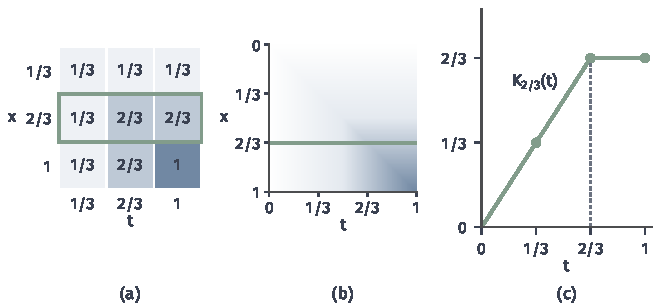
\includegraphics[width=112mm]{figures/04-spaces-measures-and-geometry/03-function-spaces/matplotlib/rkhs-kernel-as-matrix/figure.pdf}
  \caption{最小值核是一个连续下标的矩阵。(a)网格$\tfrac13,\tfrac23,1$上的矩阵$\bm K$，绿框是$x=\tfrac23$对应的行。(b)下标连成一片后的二元函数$\min(t,x)$，绿线是同一行。(c)沿绿线读出的函数就是核截面$K_{2/3}(t)=\min(t,\tfrac23)$，三个圆点是(a)中绿框内的三个数。}
  \label{fig:rkhs-kernel-as-matrix}
\end{BookInlineFigure}

类比有两处要留心。第一，有限维中$\bm K$与$\bm A$互逆，二者同样好用；无限维中通常只有$K$还是一个函数。式~\eqref{eq:rkhs-finite-difference-form}显示，网格加密时$\bm A$的元素以$1/h$的速度增长，它的极限不是二元函数，而是求导运算。所以无限维的内积一般不能用“矩阵元素”写出，我们只留下$K$。

第二，$\mathbb R^n$中每个向量都有有限长度，而函数空间中“有限长度”是实实在在的限制。$\mathbb K^X$中的绝大多数函数不属于$H$。核截面总在$H$中，标准单位向量的对应物，即只在$x$处有值的“尖峰”，却通常不在$H$中；这正是$L^2$上点值出问题的原因，读取坐标的向量在那里不存在。

\paragraph{两个例子中的核截面}

在$H_{\mathrm{aff}}$中，设$K_x=c+dt$，再生性质要求下式对一切$a,b$成立：
\[
\overline c\,a+\overline d\,b=a+bx .
\]
比较系数得$c=1$，$d=\overline x=x$。所以
\[
K_x(t)=1+xt,\qquad K(t,x)=1+tx ,
\]
称为仿射核。

图~\ref{fig:rkhs-reproducing-geometry}把这个计算画在系数平面上。核截面$K_x$对应向量$(1,x)$，读取$f=1+t$在$x=\tfrac12$处的值，就是计算$(1,1)$与$(1,\tfrac12)$的内积$1.5$。而$K_{-1}=(1,-1)$与$(1,1)$正交，对应$f(-1)=0$。函数在某点取零，几何上就是它与该点的核截面垂直。

\begin{BookInlineFigure}
  \centering
  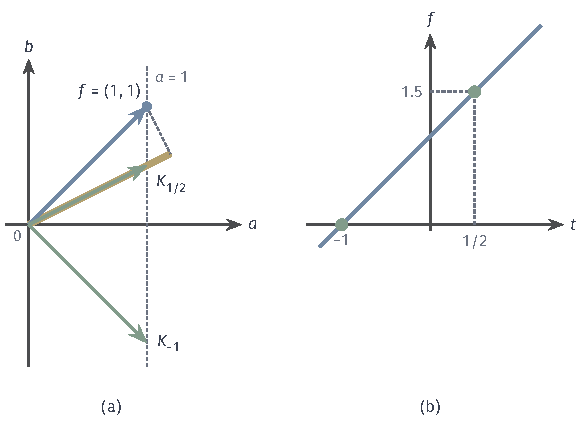
\includegraphics[width=99.4mm]{figures/04-spaces-measures-and-geometry/03-function-spaces/tikz/rkhs-reproducing-geometry/figure.pdf}
  \caption{仿射函数空间中再生性质的几何。(a)系数平面$(a,b)$与空间等距；蓝色向量是$f=1+t$，绿色向量是核截面$K_x=1+xt$，都落在虚线$a=1$上。黄色线段是$f$在$K_{1/2}$方向上的投影，其长度乘以$\lVert K_{1/2}\rVert$等于$f(1/2)=1.5$；$K_{-1}$与$f$垂直。(b)同一函数的图像，圆点标出$t=1/2$处的读数$1.5$与$t=-1$处的零点。}
  \label{fig:rkhs-reproducing-geometry}
\end{BookInlineFigure}

在$H_{\min}$中，式~\eqref{eq:rkhs-hmin-point-bound}的推导已经把$f(x)$写成了对$f'$的积分：
\[
f(x)=\int_0^1\mathbf 1_{[0,x]}(t)\,f'(t)\,\mathrm dt .
\]
只需找一个左端为零、导数为$\mathbf 1_{[0,x]}$的函数，它就是$K_x(t)=\min(t,x)$：在$[0,x]$上斜率为$1$，在$[x,1]$上保持常数$x$。

直接核对：
\[
\langle K_x,f\rangle_{H_{\min}}=\int_0^xf'(t)\,\mathrm dt=f(x) .
\]
称
\[
K(t,x)=\min(t,x)\qquad(t,x\in[0,1])
\]
为\term{最小值核}（minimum kernel）。它就是图~\ref{fig:rkhs-kernel-as-matrix}中的矩阵取遍全部下标的结果，式~\eqref{eq:rkhs-finite-difference-form}也随之成为$\int_0^1f'(t)^2\,\mathrm dt$。本章反复使用这个例子，因为它的空间、核截面和谱都可以精确算出。

\paragraph{再生核的基本性质}

核值是两个核截面的内积，内积的性质于是直接转化为核的性质。下面的定理列出其中最常用的几条。

\begin{theorem}[再生核的基本性质]
\label{thm:rkhs-kernel-properties}
设$H$是$X$上的RKHS，$K$为其再生核。则：
\begin{enumerate}
\item 共轭对称：对一切$x,y\in X$，$K(y,x)=\overline{K(x,y)}$；实值情形即$K(x,y)=K(y,x)$。
\item 正定性：对任意$n\geq1$、任意点$x_1,\ldots,x_n\in X$与$c_1,\ldots,c_n\in\mathbb K$，
\begin{equation}
\sum_{i,j=1}^n\overline{c_i}\,c_j\,K(x_i,x_j)=\Bigl\lVert\sum_{j=1}^nc_jK_{x_j}\Bigr\rVert_H^2\geq0 .
\label{eq:rkhs-kernel-positivity}
\end{equation}
\item 点评估的范数与核值的界：
\begin{equation}
\lVert\delta_x\rVert=\lVert K_x\rVert_H=\sqrt{K(x,x)},\qquad
\lvert K(x,y)\rvert\leq\sqrt{K(x,x)K(y,y)} .
\label{eq:rkhs-kernel-norm}
\end{equation}
\item 稠密性：核截面的有限线性组合全体$\operatorname{span}\{K_x:x\in X\}$在$H$中稠密。
\end{enumerate}
\end{theorem}

\begin{proof}
第1条来自内积的共轭对称：由式~\eqref{eq:rkhs-kernel-definition}，
\[
K(y,x)=\langle K_y,K_x\rangle=\overline{\langle K_x,K_y\rangle}=\overline{K(x,y)} .
\]

第2条把范数平方按内积对第一个变量共轭线性、对第二个变量线性展开：
\[
\Bigl\lVert\sum_jc_jK_{x_j}\Bigr\rVert^2=\sum_{i,j}\overline{c_i}\,c_j\,\langle K_{x_i},K_{x_j}\rangle=\sum_{i,j}\overline{c_i}\,c_j\,K(x_i,x_j).
\]

第3条中，Riesz表示给出$\lVert\delta_x\rVert=\lVert K_x\rVert$，而$\lVert K_x\rVert^2=\langle K_x,K_x\rangle=K(x,x)$；再对$\langle K_x,K_y\rangle$用Cauchy--Schwarz不等式，得到后一个不等式。

第4条用正交补判断。设$f\in H$与每个$K_x$正交，由再生性质，$f(x)=\langle K_x,f\rangle=0$对一切$x$成立，$f$是零函数。一个子空间的正交补只含零元时，它的闭包就是整个$H$（第~\ref{chap:function-inner-product-spaces}章的正交分解）。
\end{proof}

第2条中以$K(x_i,x_j)$为元素的矩阵$\bm G$是核截面组的\term{Gram矩阵}，在核的语境中也称\term{核矩阵}（kernel matrix）。把这个“无限大的矩阵”$K$限制到任意有限个下标，得到的子矩阵都半正定，这与上面的有限维样板一致。第1、2两条只涉及核，不涉及空间，下一节就把它们作为单独对二元函数的要求。

由第3条，单位球中的函数在$x$处的取值恰好填满半径$\sqrt{K(x,x)}$的圆盘（实值时是区间）：上界来自Cauchy--Schwarz不等式，取$f=K_x/\lVert K_x\rVert$即可达到。

所以前面关于统一常数的问题有了明确的答案。存在常数$C$使下式对一切$x$成立，
\[
\lvert f(x)\rvert\leq C\lVert f\rVert_H ,
\]
当且仅当$\sup_xK(x,x)<\infty$，最佳常数是$\sup_x\sqrt{K(x,x)}$。仿射核的对角值$1+x^2$在$\mathbb R$上无界，最小值核的对角值$x$不超过$1$，与前面直接得到的估计一致。

\section{从正定核构造空间}
\label{sec:rkhs-from-kernel}

上一节从空间出发得到核，并发现核的Gram矩阵总是半正定的。实际问题中往往反过来：人们先写下一个衡量两点相似程度的二元函数，再问它对应什么样的函数空间。

有限维中这个问题的答案已经知道。给定对称正定矩阵$\bm K$，令$\bm A=\bm K^{-1}$，就得到以$\bm K$为读坐标矩阵的内积空间。无限维中$\bm A$通常不存在，所以构造必须只用$\bm K$本身。本节证明，只要二元函数满足有限点组上的半正定条件，就存在唯一的RKHS以它为再生核。

构造分三步：先在核截面的有限线性组合上定义内积，并检查它不依赖于组合的写法；再处理长度为零的方向；最后完备化，并确认补进来的极限元素仍然是函数。

\subsection{正定核}
\label{sec:rkhs-pd-kernels}

定理~\ref{thm:rkhs-kernel-properties}的第1、2条只涉及核在有限个点上的值。把它们单独拿出来，就得到对二元函数的要求：把$K$看成下标取遍$X\times X$的矩阵，要求它的每个有限子矩阵都半正定。

\begin{definition}[正定核与严格正定核]
\label{def:rkhs-pd-kernel}
设$X$是非空集合，$K:X\times X\to\mathbb K$。若对任意$n\geq1$、任意点$x_1,\ldots,x_n\in X$与任意$c_1,\ldots,c_n\in\mathbb K$，
\begin{equation}
\sum_{i,j=1}^n\overline{c_i}\,c_j\,K(x_i,x_j)\geq0 ,
\label{eq:rkhs-pd-condition}
\end{equation}
并且在$\mathbb K=\mathbb R$时还有$K(x,y)=K(y,x)$，则称$K$为$X$上的\term{正定核}（positive definite kernel）。若进一步对任意\emph{互异}的点$x_1,\ldots,x_n$及不全为零的系数，上式严格大于零，则称$K$为\term{严格正定核}（strictly positive definite kernel）。
\end{definition}

用矩阵的语言，正定核要求每个Gram矩阵$\bm G=[K(x_i,x_j)]_{i,j}$都是Hermite半正定矩阵，严格正定核要求互异点组上的Gram矩阵都是正定矩阵，因而可逆。在复数情形，二次型对一切复系数取实值已经迫使$\bm G$是Hermite矩阵，所以不必另加对称条件；实数情形只用实系数检验，对称性必须单独要求。

“正定核”是通行的名称，但它只要求Gram矩阵\emph{半}正定，允许矩阵奇异。之所以要区分严格正定，是因为后文有限观测问题能否对任意数据求解，正取决于Gram矩阵是否可逆。定义中强调互异的点：若$x_1=x_2$，Gram矩阵的前两行相同，任何核的这个矩阵都奇异。

\paragraph{半正定但不严格正定的例子}

仿射核$K(x,y)=1+xy$由上一节的空间得到，所以是正定核。取三个互异点$-1,0,1$，Gram矩阵及其一个零向量为
\[
\bm G=\begin{bmatrix}2&1&0\\1&1&1\\0&1&2\end{bmatrix},\qquad
\bm G\begin{bmatrix}1\\-2\\1\end{bmatrix}=\bm 0 .
\]
对应的函数组合恰好是零函数：
\[
K_{-1}-2K_0+K_1=(1-t)-2+(1+t)=0 .
\]
原因是$H_{\mathrm{aff}}$只有二维，任意三个核截面必然线性相关。所以仿射核正定而不严格正定。

\paragraph{严格正定的例子}

\term{高斯核}（Gaussian kernel）是最常用的严格正定核：
\[
K_\sigma(x,y)=\exp\Bigl(-\frac{\lvert x-y\rvert^2}{2\sigma^2}\Bigr)\qquad(x,y\in\mathbb R).
\]
它的严格正定性可以直接证明。第~\ref{chap:fourier-transform}章算过Gauss函数的Fourier变换，把那里的结果作伸缩，下式对一切实数$u$成立：
\[
\exp\Bigl(-\frac{u^2}{2\sigma^2}\Bigr)=\int_{\mathbb R}\mathrm e^{\mathrm i\omega u}\,p_\sigma(\omega)\,\mathrm d\omega,\qquad
p_\sigma(\omega)=\frac{\sigma}{\sqrt{2\pi}}\mathrm e^{-\sigma^2\omega^2/2}.
\]

取互异的$x_1,\ldots,x_n$与系数$c_j$，令
\[
g(\omega)=\sum_jc_j\mathrm e^{-\mathrm i\omega x_j}.
\]
把$u=x_i-x_j$代入二次型，交换有限和与积分，被积函数恰好成为一个模平方：
\[
\sum_{i,j}\overline{c_i}\,c_j\,K_\sigma(x_i,x_j)=\int_{\mathbb R}\lvert g(\omega)\rvert^2\,p_\sigma(\omega)\,\mathrm d\omega\geq0 .
\]

若积分为零，由$p_\sigma>0$与$g$连续，$g$恒为零。对$g$在$\omega=0$处求$k$阶导数，$k=0,\ldots,n-1$，得到
\[
\sum_{j=1}^nc_j\,x_j^k=0 .
\]
这是系数矩阵为Vandermonde矩阵的齐次方程组，点互异时只有零解，所以$c_1=\cdots=c_n=0$。这就证明了高斯核严格正定。

在两个点$0,1$、$\sigma=1$上可以直接核对：Gram矩阵及其特征值为
\[
\begin{bmatrix}1&\mathrm e^{-1/2}\\\mathrm e^{-1/2}&1\end{bmatrix},\qquad
1\pm\mathrm e^{-1/2}\approx1.607,\ 0.393,
\]
两个特征值都为正。

图~\ref{fig:rkhs-gram-matrices}在五个点上比较这两种核。两者都是半正定矩阵，高斯核的五个特征值都为正，仿射核只有两个正特征值，其余为零。这幅图只检验了一个点组，严格正定性需要像上面那样对一切互异点组论证。

\begin{BookInlineFigure}
  \centering
  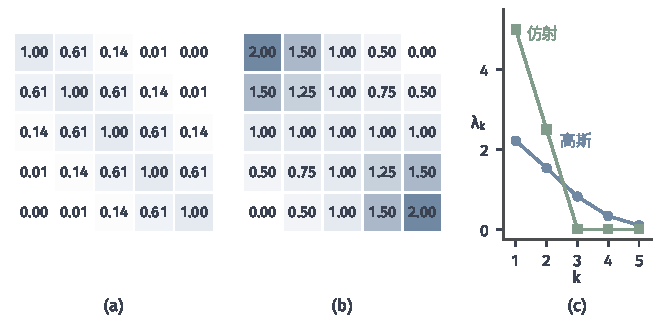
\includegraphics[width=112mm]{figures/04-spaces-measures-and-geometry/03-function-spaces/matplotlib/rkhs-gram-matrices/figure.pdf}
  \caption{点组$x=-1,-0.5,0,0.5,1$上的Gram矩阵。(a)高斯核（$\sigma=0.5$），颜色越深核值越大，数字保留两位小数（右上角的$0.00$实为$\mathrm e^{-8}\approx0.0003$）。(b)仿射核$1+xz$。(c)两个矩阵的特征值从大到小排列：高斯核为$2.217,1.531,0.820,0.333,0.099$，全为正；仿射核只有$5$与$2.5$两个正特征值。两种核都半正定，只有前者的矩阵可逆。}
  \label{fig:rkhs-gram-matrices}
\end{BookInlineFigure}

\subsection{核截面的有限线性组合}
\label{sec:rkhs-finite-combinations}

下面固定$X$上的一个正定核$K$。如果以$K$为再生核的空间存在，它必定含有全部核截面$K_x=K(\cdot,x)$，并且由式~\eqref{eq:rkhs-kernel-definition}，截面之间的内积只能是$\langle K_x,K_y\rangle=K(x,y)$。构造就从这两点出发。

\paragraph{有限维的样板：只用$\bm K$写内积}

先在有限维中看怎样不用逆矩阵写出内积。矩阵$\bm K$的列的线性组合形如$\bm K\bm c$。若$\bm K$可逆，把$\bm K\bm c$与$\bm K\bm d$代入内积，逆矩阵$\bm A$被消掉：
\[
\langle\bm K\bm c,\bm K\bm d\rangle_{\bm A}=\bm c^{\top}\bm K\bm A\bm K\bm d=\bm c^{\top}\bm K\bm d .
\]
最右端只含$\bm K$，$\bm K$奇异时照样有意义。这时同一个向量可以由不同的系数表示，$\bm K$的零向量就是长度为零的系数方向。下面的构造逐字重复这个想法。

\paragraph{半内积}

令$H_0=\operatorname{span}\{K_x:x\in X\}$，它的元素是有限和，也就是$X$上的函数：
\[
f=\sum_ia_iK_{x_i},\qquad f(t)=\sum_ia_iK(t,x_i).
\]
对这样的$f$与另一个元素$g=\sum_jb_jK_{y_j}$，按上述要求规定
\begin{equation}
\langle f,g\rangle_0=\sum_{i,j}\overline{a_i}\,b_j\,K(x_i,y_j).
\label{eq:rkhs-h0-inner}
\end{equation}
它对$g$线性、对$f$共轭线性，具有共轭对称性，并且由正定条件知$\langle f,f\rangle_0\geq0$。

问题在于，同一个函数可以有多种有限和表示，例如仿射核下$K_{-1}+K_1$与$2K_0$是同一个函数。必须先检查式~\eqref{eq:rkhs-h0-inner}的值不依赖于表示的选取。

固定$i$先对$j$求和，因为$g(x_i)=\sum_jb_jK(x_i,y_j)$，得到第一种写法。固定$j$先对$i$求和，并用$K(x_i,y_j)=\overline{K(y_j,x_i)}$，得到第二种写法：
\[
\langle f,g\rangle_0=\sum_i\overline{a_i}\,g(x_i)
=\sum_jb_j\,\overline{f(y_j)} .
\]
第一种写法只通过$g$的函数值依赖于$g$，第二种只通过$f$的函数值依赖于$f$。所以换掉$g$的表示不改变第一种写法，换掉$f$的表示不改变第二种写法，$\langle f,g\rangle_0$确实是两个\emph{函数}的量。

取$f=K_x$，第一种写法给出
\begin{equation}
\langle K_x,g\rangle_0=g(x)\qquad(g\in H_0),
\label{eq:rkhs-h0-reproducing}
\end{equation}
即再生性质在$H_0$上已经成立。

\paragraph{零范数方向的商}

现在看长度为零的方向。若把系数本身当作对象，即考虑有限支撑的系数族$a=(a_x)_{x\in X}$组成的线性空间$V$，并用式~\eqref{eq:rkhs-h0-inner}的右端定义$\langle a,b\rangle_V$，那么这只是一个半内积。仿射核的例子中，点$-1,0,1$上的系数$(1,-2,1)$非零，长度却为零。于是$\lVert a\rVert_V=\langle a,a\rangle_V^{1/2}$只是半范数，$d(a,b)=\lVert a-b\rVert_V$只是伪度量。

第~\ref{chap:metric-spaces}章对伪度量的处理是把零距离的点视为同一个点，作商空间。这里同样令
\[
N=\{a\in V:\lVert a\rVert_V=0\}.
\]
半内积的Cauchy--Schwarz不等式的证明只用到半正定性与线性，因此照样成立：
\[
\lvert\langle a,b\rangle_V\rvert\leq\lVert a\rVert_V\lVert b\rVert_V .
\]
由它可知，$a\in N$当且仅当$\langle a,b\rangle_V=0$对一切$b$成立，从而$N$是线性子空间，半内积下降到商空间$V/N$上成为真正的内积。

剩下的是把商空间与函数空间$H_0$对应起来。把系数$a$映为函数$f_a=\sum_xa_xK_x$，这个映射从$V$到$H_0$满射。记$e_t\in V$为只在$t$处取$1$、其余处取$0$的系数，则
\[
\langle e_t,a\rangle_V=\sum_xa_xK(t,x)=f_a(t),\qquad \lVert e_t\rVert_V^2=K(t,t).
\]
由半内积的Cauchy--Schwarz不等式，
\begin{equation}
\lvert f_a(t)\rvert=\lvert\langle e_t,a\rangle_V\rvert\leq\sqrt{K(t,t)}\,\lVert a\rVert_V .
\label{eq:rkhs-h0-point-bound}
\end{equation}

式~\eqref{eq:rkhs-h0-point-bound}说明，$a\in N$时$f_a$在每一点为零。反过来，$f_a\equiv0$时，
\[
\lVert a\rVert_V^2=\sum_x\overline{a_x}\,f_a(x)=0 .
\]
可见零范数的系数恰好是给出零函数的系数，商空间$V/N$与$H_0$一一对应，$\langle\cdot,\cdot\rangle_0$是$H_0$上真正的内积。把系数映成函数，恰好完成了零距离商。

\subsection{空间的完备化}
\label{sec:rkhs-completion}

$H_0$一般不完备。以最小值核为例，$H_0$由左端为零、在有限个节点处转折的连续折线组成，而下面这列折线的极限不是折线。取$m$个等距节点上核截面的平均：
\[
f_m=\frac1m\sum_{i=1}^mK_{i/m},\qquad K_{i/m}(t)=\min(t,\tfrac im).
\]
它的导数在第$k$段$(\tfrac{k-1}m,\tfrac km]$上等于$\tfrac{m-k+1}m$。

取$f(t)=t-t^2/2$，它的导数是$1-t$。在第$k$段上两个导数之差为$t-\tfrac{k-1}m$，所以
\[
\lVert f_m-f\rVert_{H_{\min}}^2=m\int_0^{1/m}u^2\,\mathrm du=\frac1{3m^2}.
\]
$(f_m)$在核范数下是Cauchy列，极限$t-t^2/2$属于$H_{\min}$，却不是折线，不在$H_0$中。下面补上这些极限，并确认它们仍然是$X$上的函数。

\paragraph{完备化与点值的极限}

由第~\ref{chap:metric-spaces}章，$H_0$有完备化$\overline{H_0}$，它由$H_0$中Cauchy列的等价类组成，$H_0$在其中稠密；内积沿Cauchy列取极限延拓过去，$\overline{H_0}$成为Hilbert空间。但完备化中的元素是抽象的等价类，还不是$X$上的函数，接下来要把它们变回函数。

点值估计~\eqref{eq:rkhs-h0-point-bound}正好提供这一步。若$(f_k)$是$H_0$中的Cauchy列，则
\[
\lvert f_k(x)-f_l(x)\rvert\leq\sqrt{K(x,x)}\,\lVert f_k-f_l\rVert_0 ,
\]
所以在每一点$f_k(x)$都是Cauchy数列，有确定的极限。两个等价的Cauchy列相差一列范数趋于零的函数，在每一点有相同的极限。用内积写出来，就是定义
\[
J:\overline{H_0}\to\mathbb K^X,\qquad (J\xi)(x)=\langle K_x,\xi\rangle_{\overline{H_0}} .
\]
若$f_k\to\xi$，则$f_k(x)=\langle K_x,f_k\rangle\to(J\xi)(x)$，所以$J\xi$就是逼近$\xi$的Cauchy列的逐点极限。由式~\eqref{eq:rkhs-h0-reproducing}，$J$在$H_0$上是恒等映射。

\paragraph{极限元素仍可识别为函数}

还剩一个危险：$\overline{H_0}$中两个不同的元素，会不会给出同一个函数？若是这样，函数之间就无法定义内积。等价地，要排除$\xi\neq0$而$J\xi$是零函数的情形。

若$\langle K_x,\xi\rangle=0$对一切$x$成立，则$\xi$与每个核截面正交，从而与它们的张成$H_0$正交。$H_0$在$\overline{H_0}$中稠密，所以$\xi$与整个空间正交，$\xi=0$。因此$J$是单射。

\begin{theorem}[由正定核确定再生核Hilbert空间]
\label{thm:rkhs-moore-aronszajn}
设$K$是非空集合$X$上的正定核。则存在唯一的RKHS，记为$H_K$，以$K$为其再生核。并且$H_0=\operatorname{span}\{K_x:x\in X\}$在$H_K$中稠密，$H_K$的每个元素都是$H_0$中某个Cauchy列的逐点极限。
\end{theorem}

\begin{proof}
先证存在性。令$H_K=J(\overline{H_0})$，规定
\[
\langle J\xi,J\eta\rangle_{H_K}=\langle\xi,\eta\rangle_{\overline{H_0}} .
\]
$J$是线性单射，这个定义良好，$J$成为等距同构，所以$H_K$是Hilbert空间；$J$的线性说明$H_K$中的加法和数乘就是逐点运算。

$J$在$H_0$上是恒等映射，故$K_x\in H_K$。对$f=J\xi$，由$J$的定义和等距性，
\[
f(x)=\langle K_x,\xi\rangle_{\overline{H_0}}=\langle JK_x,J\xi\rangle_{H_K}=\langle K_x,f\rangle_{H_K} .
\]
这就是以$K$为再生核的再生性质，点评估有界随之成立。稠密性与逐点极限的描述来自$H_0$在$\overline{H_0}$中稠密，以及上面关于$J$的讨论。

再证唯一性。设$H$是另一个以$K$为再生核的RKHS。$H$含有每个$K_x$，且$\langle K_x,K_y\rangle_H=K(x,y)$，所以$H_0\subseteq H$，两者在$H_0$上的内积一致。由定理~\ref{thm:rkhs-kernel-properties}的第4条，$H_0$在$H$中稠密。

任取$f\in H$及$H_0$中按$H$范数收敛到$f$的序列$f_k$。它是$H_0$中的Cauchy列，由再生性质逐点收敛到$f$。同一序列在$H_K$中收敛到其逐点极限，也就是$f$。所以$f\in H_K$，且
\[
\lVert f\rVert_{H_K}=\lim_k\lVert f_k\rVert_0=\lVert f\rVert_H .
\]
对调两个空间的角色，得$H=H_K$，再由极化恒等式知内积相同。
\end{proof}

这个结论通常称为Moore--Aronszajn定理\scite{aronszajn1950kernels}。图~\ref{fig:rkhs-construction-steps}用最小值核把构造的四个阶段画了出来。从此以后，“正定核”与“RKHS”可以互相确定：每个RKHS有唯一的再生核，每个正定核恰好是一个RKHS的再生核。

\begin{BookInlineFigure}
  \centering
  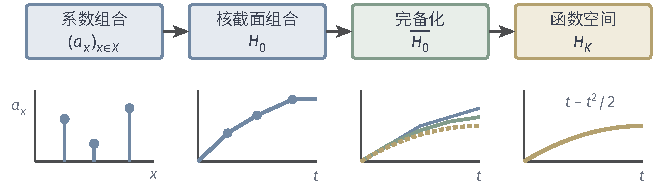
\includegraphics[width=111.1mm]{figures/04-spaces-measures-and-geometry/03-function-spaces/tikz/rkhs-construction-steps/figure.pdf}
  \caption{用最小值核走一遍由正定核构造$H_K$的四个阶段。第一栏是有限支撑的系数，二次型只给出半内积；第二栏把系数$(a_x)$变成函数$\sum_xa_xK_x$，这里是折线，零长度方向由此被商去；第三栏的蓝线、绿线是$m=2,4$时的平均折线$f_m$，虚线是它们在核范数下的极限；第四栏的$t-t^2/2$是该极限作为函数的样子，点值由Cauchy列逐点取极限得到。}
  \label{fig:rkhs-construction-steps}
\end{BookInlineFigure}

\paragraph{由最小值核重建$H_{\min}$}

以最小值核为例走一遍构造。核截面的导数是$\mathbf 1_{[0,x]}$，所以截面的内积可以写成导数的积分：
\[
\langle K_x,K_y\rangle_0=\min(x,y)=\int_0^1K_x'(t)\,K_y'(t)\,\mathrm dt .
\]
于是在$H_0$上$\lVert f\rVert_0=\lVert f'\rVert_{L^2}$。$H_0$中函数的导数恰好是区间上的阶梯函数，而阶梯函数在$L^2(0,1)$中稠密（第~\ref{chap:function-approximation}章）。于是完备化后的空间经由$f\mapsto f'$与$L^2(0,1)$等距同构，它就是上一节的$H_{\min}$。

这里唯一性起了作用：我们已经知道$H_{\min}$是以$\min(x,y)$为再生核的RKHS，定理~\ref{thm:rkhs-moore-aronszajn}保证从核出发构造的空间就是它，不必另作比较。

整个构造只用到集合$X$与核的正定性，没有用到测度或拓扑。所得的稠密性是在核范数意义下的，它不回答有限核截面组合能否逼近$H_K$之外的函数，这个问题留到第~\ref{sec:rkhs-section-span-approx}节。

\section{正定核的构造}
\label{sec:rkhs-kernel-constructions}

定理~\ref{thm:rkhs-moore-aronszajn}把问题归结为核的正定性，但直接检验一个二元函数的正定性并不方便：定义要求对一切有限点组和一切系数核验二次型。本节给出三条可操作的规则：把核写成特征向量的内积；对已知正定核作非负线性组合；对已知正定核作逐点乘积。每条规则都回到有限Gram矩阵的二次型来核验，最后用它们验证多项式核与高斯核。

\subsection{特征映射构造}
\label{sec:rkhs-feature-maps}

最常用的验证办法是把输入映到一个内积空间，再用像的内积定义核。二次型于是变成一个向量的长度平方，自然非负。

\begin{definition}[特征映射]
\label{def:rkhs-feature-map}
设$X$是非空集合，$\mathcal F$是Hilbert空间，$\Phi:X\to\mathcal F$是任意映射。称
\[
K(x,y)=\langle\Phi(x),\Phi(y)\rangle_{\mathcal F}\qquad(x,y\in X)
\]
为由$\Phi$给出的核，称$\Phi$为$K$的一个\term{特征映射}（feature map），$\mathcal F$为相应的特征空间（feature space）。
\end{definition}

由特征映射给出的核总是正定的：对任意点组与系数，
\[
\sum_{i,j}\overline{c_i}\,c_j\,K(x_i,x_j)=\Bigl\langle\sum_ic_i\Phi(x_i),\ \sum_jc_j\Phi(x_j)\Bigr\rangle_{\mathcal F}=\Bigl\lVert\sum_jc_j\Phi(x_j)\Bigr\rVert_{\mathcal F}^2\geq0 ,
\]
共轭对称性则来自内积本身。用矩阵写，若$\mathcal F=\mathbb K^d$，记$\bm\Phi$为第$i$行是$\Phi(x_i)^*$的$n\times d$矩阵，则Gram矩阵是$\bm\Phi\bm\Phi^*$。

反过来，每个正定核都有特征映射：取$\mathcal F=H_K$，$\Phi(x)=K_x$，则$\langle K_x,K_y\rangle_{H_K}=K(x,y)$。称它为\term{规范特征映射}（canonical feature map）。所以“$K$正定”与“$K$有某个特征映射”是等价的两种说法。

\paragraph{线性核与有限特征核}

在$\mathbb R^d$上，取$\Phi(\bm x)=\bm x$，得到\term{线性核}（linear kernel）$K(\bm x,\bm y)=\bm x^{\top}\bm y$。在$\mathbb R$上，展开平方可得
\[
(1+xy)^2=1+2xy+x^2y^2=\bigl\langle(1,\sqrt2\,x,x^2),\ (1,\sqrt2\,y,y^2)\bigr\rangle ,
\]
所以二次多项式核是三维特征向量的内积核。这类由有限个特征分量给出的核称为有限特征核，它们的Gram矩阵秩不超过特征维数，因而在点数超过特征维数时一定奇异。

\paragraph{特征维数与RKHS}

同一个核可以有许多不同的特征映射。仿射核$1+xy$既可以由$\Phi_1(x)=(1,x)\in\mathbb R^2$给出，也可以由$\Phi_2(x)=(1,x/\sqrt2,x/\sqrt2)\in\mathbb R^3$给出，因为$1+\tfrac{xy}{2}+\tfrac{xy}{2}=1+xy$。特征空间的维数和坐标都不同，核却相同，由核确定的RKHS也相同。所以特征维数不是空间的性质，RKHS中的函数及其范数要从核读出。

下面说明怎样从任何一个特征映射读出RKHS。给定$\Phi:X\to\mathcal F$，每个参数$w\in\mathcal F$确定一个函数
\[
f_w(x)=\langle\Phi(x),w\rangle_{\mathcal F}.
\]
令$V$为$\{\Phi(x):x\in X\}$张成的闭子空间，$P_V$为到$V$的正交投影。$w-P_Vw$与每个$\Phi(x)$正交，所以$f_w=f_{P_Vw}$：$V^\perp$中的参数分量对函数没有任何影响。

\begin{theorem}[特征映射给出的RKHS]
\label{thm:rkhs-feature-space}
设$\Phi:X\to\mathcal F$是正定核$K$的特征映射，$V$为$\Phi(X)$张成的闭子空间。则
\begin{equation*}
\begin{gathered}
H_K=\{f_w:w\in\mathcal F\},\\
\lVert f_w\rVert_{H_K}=\lVert P_Vw\rVert_{\mathcal F}=\min\{\lVert u\rVert_{\mathcal F}:u\in\mathcal F,\ f_u=f_w\} ,
\end{gathered}
\end{equation*}
并且$w\mapsto f_w$限制在$V$上是从$V$到$H_K$的等距同构。
\end{theorem}

\begin{proof}
线性映射$A:w\mapsto f_w$的核是$\{w:\langle\Phi(x),w\rangle=0,\ \forall x\}=V^\perp$，所以$A$在$V$上是单射，且$A(\mathcal F)=A(V)$。令$H=A(\mathcal F)$，规定$\langle Aw,Au\rangle_H=\langle P_Vw,P_Vu\rangle_{\mathcal F}$，则$A|_V$是等距同构，$H$作为闭子空间$V$的等距像是Hilbert空间，运算是逐点的。

令$k_x=A\Phi(x)$。因$\Phi(x)\in V$，有$\langle k_x,f_w\rangle_H=\langle\Phi(x),P_Vw\rangle=\langle\Phi(x),w\rangle=f_w(x)$；而$k_x(y)=\langle\Phi(y),\Phi(x)\rangle=K(y,x)$，即$k_x=K_x$。所以$H$是以$K$为再生核的RKHS，由定理~\ref{thm:rkhs-moore-aronszajn}的唯一性，$H=H_K$。最后，$f_u=f_w$当且仅当$u-w\in V^\perp$，此时$P_Vu=P_Vw$，而$\lVert u\rVert\geq\lVert P_Vu\rVert$，等号在$u\in V$时取得。
\end{proof}

定理的最后一个等式说明：在冗余的特征表示中，任意一个能给出$f$的参数，其长度只是$\lVert f\rVert_{H_K}$的上界；只有落在$V$中的参数，长度才等于函数的范数。

\begin{example}[冗余特征]
\label{ex:rkhs-redundant-features}
取$\Phi(x)=(x,x)\in\mathbb R^2$，核为$K(x,y)=2xy$。$V$是直线$\operatorname{span}\{(1,1)\}$，正交补方向是$(1,-1)$。参数$(2,0)$、$(1,1)$、$(0,2)$都给出同一函数$f(x)=2x$，长度分别为$2$、$\sqrt2$、$2$；由定理~\ref{thm:rkhs-feature-space}，$\lVert f\rVert_{H_K}=\sqrt2$，是$(2,0)$在$V$上的投影$(1,1)$的长度，见图~\ref{fig:rkhs-visible-parameters}。

直接核对：$H_K$由$f(x)=cx$组成，核截面$K_x(t)=2xt$，再生性质要求$\langle 2xt,ct\rangle=cx$，故$\langle at,ct\rangle_{H_K}=ac/2$，$\lVert 2x\rVert_{H_K}^2=4/2=2$，结果一致。特征空间是二维的，RKHS却是一维的。
\end{example}

\begin{figure}[!htb]
  \centering
  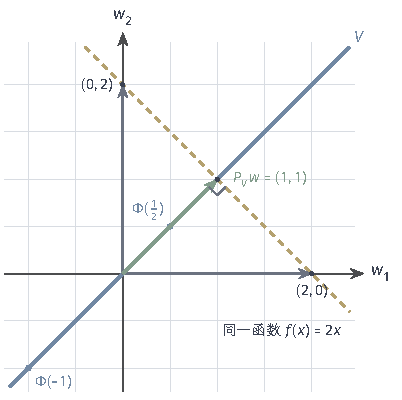
\includegraphics[width=68.1mm]{figures/02-abstract-mathematics/03-function-spaces/tikz/c5-visible-parameters/figure.pdf}
  \caption{冗余特征$\Phi(x)=(x,x)$的参数平面。各点的特征$\Phi(x)$都落在蓝色直线$V$上；黄色虚线上的参数都给出同一函数$f(x)=2x$。其中与$V$相交的$P_Vw=(1,1)$长度最短，为$\sqrt2$，这就是$\lVert f\rVert_{H_K}$；$(2,0)$与$(0,2)$长度为$2$，多出的部分来自对函数没有影响的$V^\perp$方向。}
  \label{fig:rkhs-visible-parameters}
\end{figure}

对仿射核的两个特征映射，$\Phi_1$的$V$是整个$\mathbb R^2$，所以$\lVert a+bt\rVert_{H_K}^2=a^2+b^2$，与第~\ref{sec:rkhs-evaluation-bounds}节一致。$\Phi_2$的$V$是$\operatorname{span}\{(1,0,0),(0,1,1)/\sqrt2\}$，参数$(a,b/\sqrt2,b/\sqrt2)$给出$a+bt$，长度同样是$\sqrt{a^2+b^2}$；参数$(a,\sqrt2\,b,0)$也给出同一函数，长度$\sqrt{a^2+2b^2}$却更大。

\subsection{非负线性组合}
\label{sec:rkhs-nonnegative-combinations}

特征映射适合验证可以写成内积的核。更多的核由几个已知核组合得到，只要组合方式保持正定性，就不必为每个新核重新寻找特征映射。最简单的组合是加权求和。

\begin{theorem}[非负线性组合]
\label{thm:rkhs-nonnegative-combination}
设$K_1,\ldots,K_m$是$X$上的正定核，$\alpha_1,\ldots,\alpha_m\geq0$是非负实数。则$K=\sum_l\alpha_lK_l$是$X$上的正定核。
\end{theorem}

\begin{proof}
固定点组与系数向量$\bm c$，记$\bm G_l$为$K_l$的Gram矩阵，则$K$的Gram矩阵是$\sum_l\alpha_l\bm G_l$，且
\[
\bm c^*\Bigl(\sum_l\alpha_l\bm G_l\Bigr)\bm c=\sum_l\alpha_l\,\bm c^*\bm G_l\bm c\geq0 ,
\]
因为每一项都是非负数与非负数之积。实数情形下对称性显然保持。
\end{proof}

用特征映射表达，若$\Phi_l$是$K_l$的特征映射，把$\sqrt{\alpha_l}\,\Phi_l(x)$依次拼接成直和空间$\mathcal F_1\oplus\cdots\oplus\mathcal F_m$中的一个向量，其内积正是$\sum_l\alpha_lK_l(x,y)$。例如仿射核$1+xy$是常数核$1$（特征为常数$1$）与线性核$xy$之和，拼接特征就是前面的$\Phi_1(x)=(1,x)$。

系数的符号不能任意改变。仿射核减去常数核$2$得到$xy-1$，它在$x=y=0$处的值为$-1$；而正定核在单点上的Gram矩阵是$1\times1$矩阵$[K(x,x)]$，必须非负。所以两个正定核之差一般不是正定核。复系数同样不行：$\mathrm iK$的对角值是纯虚数，二次型不再取实值。

\subsection{逐点乘积}
\label{sec:rkhs-pointwise-products}

第二种组合是逐点相乘。这时乘积核的Gram矩阵是两个Gram矩阵的逐元素乘积，正定性来自卷二的Schur乘积定理：两个同阶Hermite半正定矩阵的逐元素乘积仍是Hermite半正定矩阵，可参考\BookChapterRef{chap:normed-inner-product-spaces}{卷二第3章“赋范空间与内积空间”}。其机制是把两组向量的内积相乘，等于它们张量积之间的内积。

\begin{theorem}[逐点乘积]
\label{thm:rkhs-pointwise-product}
设$K_1,K_2$是同一集合$X$上的正定核。则$K(x,y)=K_1(x,y)K_2(x,y)$是$X$上的正定核。若$\Phi_1,\Phi_2$分别是$K_1,K_2$取值于$\mathbb K^{d_1},\mathbb K^{d_2}$的特征映射，则$\Phi_1(x)\otimes\Phi_2(x)\in\mathbb K^{d_1d_2}$是$K$的特征映射。
\end{theorem}

\begin{proof}
固定点组，$K$的Gram矩阵是$\bm G_1\odot\bm G_2$，由Schur乘积定理它是Hermite半正定矩阵，所以$K$正定。对特征映射，按坐标展开$\langle u\otimes v,u'\otimes v'\rangle=\sum_{k,l}\overline{u_kv_l}\,u_k'v_l'=\langle u,u'\rangle\langle v,v'\rangle$，取$u=\Phi_1(x)$、$v=\Phi_2(x)$、$u'=\Phi_1(y)$、$v'=\Phi_2(y)$即得。
\end{proof}

\paragraph{两条辅助规则}

验证常见的连续核，还需要两条与乘积相关的简单规则。第一条是函数缩放：对任意$g:X\to\mathbb K$，$g(x)\overline{g(y)}$是正定核，因为
\[
\sum_{i,j}\overline{c_i}\,c_j\,g(x_i)\overline{g(x_j)}=\Bigl\lvert\sum_i\overline{c_i}\,g(x_i)\Bigr\rvert^2\geq0 ;
\]
于是由定理~\ref{thm:rkhs-pointwise-product}，$g(x)\overline{g(y)}K(x,y)$对任意正定核$K$仍正定。第二条是逐点极限：若正定核$K^{(k)}$在每个$(x,y)$处收敛到$K(x,y)$，则$K$正定，因为每个有限二次型都是非负数的极限。

\paragraph{多项式核与高斯核}

由这几条规则可以验证常用的核。常数$c\geq0$是以$\sqrt c$为特征的核，所以$c+\bm x^{\top}\bm y$正定（定理~\ref{thm:rkhs-nonnegative-combination}），它的$p$次幂即\term{多项式核}（polynomial kernel）$(c+\bm x^{\top}\bm y)^p$也正定（定理~\ref{thm:rkhs-pointwise-product}反复使用）。

$\mathbb R^d$上的高斯核$K_\sigma(\bm x,\bm y)=\exp\bigl(-\lVert\bm x-\bm y\rVert_2^2/(2\sigma^2)\bigr)$分三步验证。先展开指数中的平方：
\[
\exp\Bigl(-\frac{\lVert\bm x-\bm y\rVert_2^2}{2\sigma^2}\Bigr)
=g(\bm x)\,g(\bm y)\,\exp\Bigl(\frac{\bm x^{\top}\bm y}{\sigma^2}\Bigr),\qquad
g(\bm x)=\exp\Bigl(-\frac{\lVert\bm x\rVert_2^2}{2\sigma^2}\Bigr).
\]
再看中间因子：部分和$\sum_{k=0}^N(\bm x^{\top}\bm y)^k/(k!\,\sigma^{2k})$是线性核各次幂的非负组合，因而正定；指数级数逐点收敛，由逐点极限规则，$\exp(\bm x^{\top}\bm y/\sigma^2)$正定。最后由函数缩放规则乘上$g(\bm x)g(\bm y)$。这样得到的是正定性；严格正定性是更强的性质，第~\ref{sec:rkhs-pd-kernels}节已经说明它需要另外的论证。

\paragraph{运算在核截面上的效果}

核的运算直接作用在核截面上：和核的截面是两个截面之和，乘积核的截面是两个截面之积。图~\ref{fig:rkhs-kernel-operations}在$x=0.4$处比较仿射核与高斯核（$\sigma=0.3$）。和核的截面在仿射趋势上叠加了一个局部隆起；乘积核的截面仍集中在$x$附近，但被仿射因子$1+0.4t$拉得右高左低。所以乘积核对应空间中的函数同时带有两种核的特点：局部性来自高斯因子，倾斜来自仿射因子。

\begin{figure}[!htb]
  \centering
  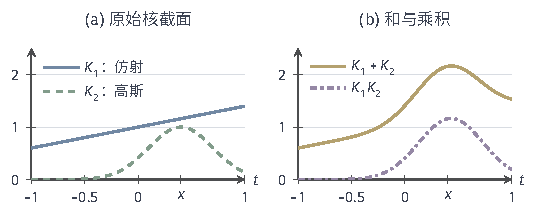
\includegraphics[width=90.7mm]{figures/02-abstract-mathematics/03-function-spaces/tikz/c5-kernel-operations/figure.pdf}
  \caption{核运算在核截面上的效果，固定$x=0.4$，$t\in[-1,1]$。(a)~仿射核截面$1+0.4t$与高斯核截面（$\sigma=0.3$）；(b)~两者之和与逐点乘积。和核的截面是两个截面相加，乘积核的截面是两个截面相乘，仍保持以$x$为中心的局部形状。}
  \label{fig:rkhs-kernel-operations}
\end{figure}

本节的规则都从已知的核或已知的特征出发。还有一种重要的特征来自核本身的谱：在定义域上加入测度后，核积分算子的特征函数给出一组按特征值加权的特征，这要用到算子的谱理论，在第~\ref{sec:rkhs-mercer}节另行构造。

\section{最小范数插值}
\label{sec:rkhs-min-norm-interpolation}

现在回到第~\ref{sec:rkhs-recovery}节的精确插值问题，把候选空间取为RKHS。固定$X$上的RKHS $H$及其再生核$K$，取观测位置$x_1,\ldots,x_n\in X$（暂不要求互异）和读数$\bm y\in\mathbb K^n$，要找$f\in H$使$f(x_i)=y_i$对每个$i$成立。

这个问题要分两步回答。第一步判断数据能否由$H$中的函数实现；若不能，谈论“最好的插值”没有意义。第二步在可行函数中选出范数最小的一个。两步都依赖同一个正交分解：把$H$分成读数能看见的有限维部分与读数完全看不见的部分。

\subsection{观测映射}
\label{sec:rkhs-observation-map}

把$n$个读数合在一起，得到线性映射
\[
S:H\to\mathbb K^n,\qquad Sf=\bigl(f(x_1),\ldots,f(x_n)\bigr)^{\top},
\]
称为\term{观测映射}（observation map）。精确插值就是解方程$Sf=\bm y$。由再生性质，$Sf$的第$i$个分量是$\langle K_{x_i},f\rangle$，所以$S$是有界线性映射，并且$\lVert Sf\rVert_2^2\leq\bigl(\sum_iK(x_i,x_i)\bigr)\lVert f\rVert_H^2$。

\paragraph{伴随与Gram矩阵}

$\mathbb K^n$取标准内积$\langle\bm c,\bm d\rangle=\bm c^*\bm d$。对任意$\bm c\in\mathbb K^n$，
\[
\langle\bm c,Sf\rangle=\sum_i\overline{c_i}\,f(x_i)=\sum_i\overline{c_i}\,\langle K_{x_i},f\rangle_H=\Bigl\langle\sum_ic_iK_{x_i},\ f\Bigr\rangle_H ,
\]
所以$S$的伴随把系数映成核截面的组合：$S^*\bm c=\sum_ic_iK_{x_i}$。这类函数的读数和内积都可以用Gram矩阵$\bm G_{i,j}=K(x_i,x_j)$计算：
\begin{equation}
S(S^*\bm c)=\bm G\bm c,\qquad
\langle S^*\bm c,S^*\bm d\rangle_H=\bm c^*\bm G\bm d,\qquad
SS^*=\bm G .
\label{eq:rkhs-gram-calculus}
\end{equation}
第一式的第$i$个分量是$\sum_jc_jK(x_i,x_j)$，第二式由$\langle K_{x_i},K_{x_j}\rangle=K(x_i,x_j)$展开得到。于是在核截面的张成空间内，函数的全部计算都化为$n$维向量与$n\times n$矩阵的计算。注意$\bm c^*\bm G\bm c$才是函数的范数平方，系数的欧氏长度$\lVert\bm c\rVert_2$一般与函数范数无关。

\paragraph{秩与线性相关}

$\bm G$的秩恰好是核截面$K_{x_1},\ldots,K_{x_n}$张成空间的维数。因为$\bm G$是Hermite半正定矩阵，$\bm c^*\bm G\bm c=0$当且仅当$\bm G\bm c=\bm 0$；而由式~\eqref{eq:rkhs-gram-calculus}，$\bm c^*\bm G\bm c=\lVert S^*\bm c\rVert_H^2$。所以$\ker\bm G=\ker S^*$，即$\bm G\bm c=\bm 0$恰好描述核截面之间的线性关系，由秩—零度公式即得上述结论。

$\bm G$奇异有三种典型来源。一是重复观测：若$x_1=x_2$，则$K_{x_1}=K_{x_2}$，$\bm G$的前两行相同。二是核截面所在的空间维数不够：仿射核在$-1,0,1$上的Gram矩阵以$(1,-2,1)^{\top}$为零向量，因为二维空间中三个截面必然线性相关。三是退化的观测点：最小值核满足$K_0=\min(\cdot,0)=0$，$H_{\min}$中所有函数在$0$处取零，含有$x=0$的观测点组，Gram矩阵有一整行为零。

\begin{example}[最小值核的观测映射]
\label{ex:rkhs-hmin-observation}
在$H_{\min}$中取$x_1,x_2,x_3=\tfrac13,\tfrac23,1$，Gram矩阵为
\[
\bm G=\frac13\begin{bmatrix}1&1&1\\1&2&2\\1&2&3\end{bmatrix},\qquad
\det\bm G=\frac1{27}\neq0 .
\]
三个核截面线性无关，它们的组合$S^*\bm c=\sum_jc_j\min(\cdot,x_j)$恰好是左端为零、只在$\tfrac13,\tfrac23$处转折的连续折线：在三段上的斜率依次为$c_1+c_2+c_3$、$c_2+c_3$、$c_3$。
\end{example}

\subsection{观测零空间}
\label{sec:rkhs-observation-null-space}

读数看不见的函数组成$S$的核
\[
N=\ker S=\{f\in H:f(x_1)=\cdots=f(x_n)=0\},
\]
称为\term{观测零空间}（observation null space）。$S$有界，所以$N$是闭子空间。记$M=\operatorname{span}\{K_{x_1},\ldots,K_{x_n}\}$，它是$S^*$的像，有限维因而闭。下面的定理说明这两个子空间互为正交补。

\begin{theorem}[观测零空间的正交补]
\label{thm:rkhs-observation-null-space}
在上述记号下，$N=M^\perp$，$N^\perp=M$，从而$H=M\oplus N$。记$P$为到$M$的正交投影，则对一切$f\in H$，$S(Pf)=Sf$且$\lVert Pf\rVert_H\leq\lVert f\rVert_H$。两个函数$f,g$在全部观测点上读数相同，当且仅当$f-g\in N$，也当且仅当$Pf=Pg$。
\end{theorem}

\begin{proof}
$f\in N$当且仅当$\langle K_{x_i},f\rangle=0$对每个$i$成立，即$f$与$M$的每个生成元正交，这就是$N=M^\perp$。$M$是闭子空间，所以$N^\perp=M^{\perp\perp}=M$，正交分解$H=M\oplus N$由第~\ref{chap:inner-product-spaces}章的投影定理给出。$f-Pf\in N$说明$S(f-Pf)=0$；勾股定理给出$\lVert f\rVert^2=\lVert Pf\rVert^2+\lVert f-Pf\rVert^2$。最后，$Sf=Sg$等价于$f-g\in N$，而由正交分解，这又等价于$P(f-g)=0$。
\end{proof}

所以有限个点值恰好确定投影$Pf$，余项$f-Pf$完全看不见：它在每个观测点取零，不论多大都不改变任何读数。

\begin{example}[折线与观测零空间的正交性]
\label{ex:rkhs-hmin-null-space}
继续例~\ref{ex:rkhs-hmin-observation}。$N$由$H_{\min}$中在$\tfrac13,\tfrac23,1$处取零的函数组成，例如$\sin(3k\pi x)$（$k=1,2,\ldots$），所以$N$是无限维的。$M$是左端为零、以$\tfrac13,\tfrac23$为节点的折线。

正交性可以直接验证：设$h\in M$在第$k$段上的斜率为$s_k$，$g\in N$，则
\[
\langle h,g\rangle_{H_{\min}}=\int_0^1h'g'=\sum_{k=1}^3s_k\bigl(g(\tfrac k3)-g(\tfrac{k-1}3)\bigr)=0 ,
\]
因为$g$在四个节点$0,\tfrac13,\tfrac23,1$上都取零。在这个例子中，$Pf$就是过原点和三个观测点的折线插值。
\end{example}

定理~\ref{thm:rkhs-observation-null-space}还有一个更一般的推论。若某个准则只通过读数$Sf$依赖于$f$，再加上一项随$\lVert f\rVert_H$增大的惩罚，那么把$f$换成$Pf$不改变前者、不增大后者，最优函数总可以取在有限维空间$M$中，即写成$\sum_jc_jK_{x_j}$的形式。这就是带损失与正则项的函数拟合中表示定理的结构依据，可参考\BookChapterRef{chap:function-fitting-regularization}{卷五第10章“函数拟合与正则化”}。本章只讨论精确插值这一特殊情形。

\subsection{约束相容性}
\label{sec:rkhs-consistency}

给定读数$\bm y$，第一步要判断是否存在$f\in H$满足$Sf=\bm y$。不是任意数据都能被插值：在重复观测点上给出两个不同的读数，任何函数都无法同时满足。下面的定理把可行性写成矩阵条件。

\begin{theorem}[插值约束的相容性]
\label{thm:rkhs-consistency}
存在$f\in H$使$Sf=\bm y$，当且仅当$\bm y$属于$\bm G$的像，也当且仅当$\bm d^*\bm y=0$对一切$\bm d\in\ker\bm G$成立。
\end{theorem}

\begin{proof}
若$Sf=\bm y$，由定理~\ref{thm:rkhs-observation-null-space}，$\bm y=S(Pf)$，而$Pf\in M$可写成$S^*\bm c$，于是$\bm y=SS^*\bm c=\bm G\bm c$。反过来，若$\bm y=\bm G\bm c$，则$f=S^*\bm c$满足$Sf=\bm y$。$\bm G$是Hermite矩阵，其像是$\ker\bm G$的正交补，这给出第二个等价条件。
\end{proof}

当$\bm G$可逆时，像是整个$\mathbb K^n$，任意数据都可以插值；特别地，严格正定核在互异观测点上总是如此。当$\bm G$奇异时，数据必须满足$\ker\bm G$给出的线性关系。仿射核在$-1,0,1$上，$\ker\bm G$由$(1,-2,1)^{\top}$张成，相容条件是$y_1-2y_2+y_3=0$，即三个数据点共线。读数$(0,1,0)$不满足它，所以没有仿射函数通过这三点；这与第~\ref{sec:rkhs-finite-feature-space}节例~\ref{ex:rkhs-polynomial-features}的第1种情形是同一现象，只是那里用设计矩阵的列空间来判断。重复观测$x_1=x_2$时$(1,-1,0,\ldots,0)^{\top}\in\ker\bm G$，相容条件是$y_1=y_2$；$H_{\min}$中在$0$处观测时，相容条件是该读数为零。

还要区分“没有插值函数”与“插值函数不止一个”，二者由不同的对象决定。前者取决于$\bm y$是否落在$\bm G$的像中；后者取决于观测零空间$N$是否非零，与$\bm G$是否可逆无关。仿射核在$-1,0,1$上$\bm G$奇异，但三个截面已经张成整个$H_{\mathrm{aff}}$，$N=\{0\}$，相容数据确定唯一的函数。$H_{\min}$中三个观测点给出可逆的$\bm G$，任何数据都可行，$N$却是无限维的，可行函数有无穷多个。所以不能把$\bm G$奇异理解为插值不唯一，也不能把$\bm G$可逆理解为函数被唯一确定。

\subsection{最小范数解}
\label{sec:rkhs-min-norm-solution}

数据相容时，可行函数组成仿射集$f_0+N$，其中$f_0$是任意一个可行函数。第~\ref{sec:rkhs-finite-feature-space}节在有限特征空间中遇到解不唯一时，卷二的做法是选欧氏长度最小的系数；在RKHS中，自然的做法是选范数最小的函数。

\begin{theorem}[最小范数插值]
\label{thm:rkhs-min-norm-interpolation}
设$\bm y$属于$\bm G$的像，$\bm c$是方程$\bm G\bm c=\bm y$的任意一个解，令
\[
f^+=S^*\bm c=\sum_{j=1}^nc_jK_{x_j},\qquad f^+(x)=\sum_{j=1}^nc_jK(x,x_j).
\]
则$f^+$不依赖于解$\bm c$的选取，它是$M$中唯一满足$Sf=\bm y$的函数；对任意满足$Sg=\bm y$的$g\in H$，
\begin{equation}
\lVert g\rVert_H^2=\lVert f^+\rVert_H^2+\lVert g-f^+\rVert_H^2 ,
\label{eq:rkhs-min-norm-pythagoras}
\end{equation}
所以$f^+$是唯一的最小范数可行函数，并且$\lVert f^+\rVert_H^2=\bm c^*\bm y=\bm y^*\bm G^{\dagger}\bm y$，其中$\bm G^{\dagger}$是Moore--Penrose伪逆。
\end{theorem}

\begin{proof}
由式~\eqref{eq:rkhs-gram-calculus}，$Sf^+=\bm G\bm c=\bm y$，所以$f^+$可行。若$\bm c'$是另一个解，则$\bm G(\bm c-\bm c')=\bm 0$，由上一小节$S^*(\bm c-\bm c')=0$，两组系数给出同一函数。$M$中两个读数相同的函数之差属于$M\cap N=\{0\}$，这给出$M$中的唯一性。

对可行的$g$，$g-f^+\in N$，而$f^+\in M=N^\perp$，勾股定理即为式~\eqref{eq:rkhs-min-norm-pythagoras}，等号仅在$g=f^+$时成立。最后，$\lVert f^+\rVert^2=\bm c^*\bm G\bm c=\bm c^*\bm y$；取$\bm c=\bm G^{\dagger}\bm y$是方程的一个解（$\bm y$在$\bm G$的像中），代入并用$\bm G^{\dagger}$为Hermite矩阵，得$\bm y^*\bm G^{\dagger}\bm y$。
\end{proof}

称$f^+$为数据的\term{最小范数插值}（minimum-norm interpolation）。由定理~\ref{thm:rkhs-observation-null-space}，它也是任意可行函数在$M$上的投影。整个求解只需要核在观测点上的值：解一个$n\times n$的线性方程，再用核截面组合出函数。

\paragraph{系数不唯一与函数唯一}

定理区分了两种唯一性。$\bm G$奇异时，方程$\bm G\bm c=\bm y$的解组成$\bm c_0+\ker\bm G$，系数不唯一；但$\ker\bm G$中的系数给出零函数，所以函数$f^+$唯一。伪逆从全部解中挑出欧氏长度最小的系数，这只是选了一种写法，与函数范数最小是两回事。

仿射核在$-1,0,1$上，取相容数据$\bm y=(0,1,2)^{\top}$。$\bm c=(0,0,1)^{\top}$是一个解，全部解为$(s,-2s,1+s)^{\top}$。无论$s$取何值，$f^+=sK_{-1}-2sK_0+(1+s)K_1=1+t$，范数平方$\bm c^*\bm y=-2s+2(1+s)=2=1^2+1^2$。

\begin{example}[最小值核的折线插值]
\label{ex:rkhs-hmin-interpolation}
在例~\ref{ex:rkhs-hmin-observation}的观测点上，取$q(x)=4x(1-x)$的读数$\bm y=(\tfrac89,\tfrac89,0)^{\top}$。由定理~\ref{thm:rkhs-min-norm-interpolation}与例~\ref{ex:rkhs-hmin-null-space}，$f^+$是过原点和三个数据点的折线，三段斜率依次为$\tfrac83,0,-\tfrac83$。对照例~\ref{ex:rkhs-hmin-observation}中的斜率公式，得$\bm c=(\tfrac83,\tfrac83,-\tfrac83)^{\top}$。

代回检验$\bm G\bm c=\bm y$：第一行$\tfrac13\cdot\tfrac83=\tfrac89$，第二行$\tfrac13(\tfrac83+\tfrac{16}3-\tfrac{16}3)=\tfrac89$，第三行$\tfrac13(\tfrac83+\tfrac{16}3-8)=0$。范数为$\lVert f^+\rVert^2=\bm c^{\top}\bm y=\tfrac{128}{27}$，也等于折线导数的平方积分$2\cdot\tfrac13\cdot\tfrac{64}{9}$。而$\lVert q\rVert_{H_{\min}}^2=\int_0^1(4-8x)^2\,\mathrm dx=\tfrac{16}3=\tfrac{144}{27}$，由式~\eqref{eq:rkhs-min-norm-pythagoras}，$\lVert q-f^+\rVert^2=\tfrac{16}{27}$。
\end{example}

最小范数插值只回答了“在可行函数中选哪一个”。它在测点之间与真实函数相差多少，取决于真实函数在$N$中的分量，这是读数看不见的部分。下一节在已知目标函数的前提下研究这种表示误差，并看它怎样随子空间的扩大而变化。

\section{有限维子空间逼近}
\label{sec:rkhs-finite-subspaces}

上一节从读数出发，目标函数未知，问题是在可行函数中选一个。本节换一个角度：目标函数$f\in H$已知，或者至少它与若干固定函数的内积可以算出，我们只允许用一个有限维子空间$V\subseteq H$中的函数来表示它。问题变成表示误差：$V$中离$f$最近的函数是谁，误差有多大，$V$逐步扩大后误差能否趋于零。

在Hilbert空间中，离$f$最近的元素就是正交投影$P_Vf$，误差为$\lVert f-P_Vf\rVert_H$（第~\ref{chap:function-inner-product-spaces}章）。RKHS的额外结构是，这个范数误差还能控制每一点的误差，而控制的系数只依赖于核与子空间，不依赖于$f$。

\begin{theorem}[子空间的再生核与逐点误差]
\label{thm:rkhs-subspace-error}
设$V$是RKHS $H$的闭子空间，$P_V$为到$V$的正交投影。则$V$带着$H$的内积是RKHS，其再生核为$K_V(x,y)=\langle P_VK_x,P_VK_y\rangle_H$；并且对一切$f\in H$与$x\in X$，
\begin{equation}
\lvert f(x)-(P_Vf)(x)\rvert\leq\sqrt{K(x,x)-K_V(x,x)}\ \lVert f-P_Vf\rVert_H .
\label{eq:rkhs-subspace-pointwise}
\end{equation}
\end{theorem}

\begin{proof}
对$g\in V$，$g(x)=\langle K_x,g\rangle=\langle P_VK_x,g\rangle$，所以$V$中$x$处的核截面是$P_VK_x$，再生核为式中所写。

令$r=f-P_Vf\in V^\perp$。$P_VK_x\in V$与$r$正交，所以
\[
r(x)=\langle K_x,r\rangle=\langle K_x-P_VK_x,r\rangle .
\]
用Cauchy--Schwarz不等式，并由勾股定理计算第一个因子：
\[
\lVert K_x-P_VK_x\rVert^2=\lVert K_x\rVert^2-\lVert P_VK_x\rVert^2=K(x,x)-K_V(x,x).
\]
这就是式~\eqref{eq:rkhs-subspace-pointwise}。
\end{proof}

式~\eqref{eq:rkhs-subspace-pointwise}右端的第一个因子是核截面$K_x$中不能由$V$表示的部分的长度，它只取决于核与子空间；第二个因子是$f$本身的表示误差。下面分别考察两类有限子空间：由核截面张成的子空间，以及由一般有限特征张成的子空间。

\subsection{核截面张成空间的逼近}
\label{sec:rkhs-section-span-approx}

取有限点组$Z=\{x_1,\ldots,x_n\}$，$V=M_Z=\operatorname{span}\{K_x:x\in Z\}$。由上一节，$P_{M_Z}f$就是$f$在$Z$上读数的最小范数插值，只需$f$的点值就能算出。这时式~\eqref{eq:rkhs-subspace-pointwise}中的第一个因子记为$P_Z(x)$，称为\term{核插值幂函数}（power function）。

$P_{M_Z}K_x$是$K_x$读数$\bm k_Z(x)=(K(x_1,x),\ldots,K(x_n,x))^{\top}$的最小范数插值，由定理~\ref{thm:rkhs-min-norm-interpolation}，
\begin{equation}
P_Z(x)^2=K(x,x)-\bm k_Z(x)^*\bm G^{\dagger}\bm k_Z(x).
\label{eq:rkhs-power-function}
\end{equation}
用矩阵的话说，这是$\bm K$关于观测下标的Schur补的对角元。它在每个观测点处为零，在观测点之间随间隔增大而增大。

\paragraph{点集决定的稠密性}

定理~\ref{thm:rkhs-kernel-properties}已经说明，全部核截面的组合在$H$中稠密，所以任何$f\in H$都能被有限个截面的组合任意逼近。实际中可选的位置往往受限，例如只能在一个点集$D\subseteq X$上放置截面。这时稠密性由下面的条件刻画。

\begin{theorem}[限定点集的核截面稠密性]
\label{thm:rkhs-dense-sections}
设$D\subseteq X$。则$\operatorname{span}\{K_x:x\in D\}$在$H$中稠密，当且仅当$H$中在$D$上处处为零的函数只有零函数。
\end{theorem}

\begin{proof}
由再生性质，$f$与每个$K_x$（$x\in D$）正交，当且仅当$f$在$D$上处处为零。一个子空间在Hilbert空间中稠密，当且仅当与它正交的元素只有零元。
\end{proof}

这个条件同时涉及核与点集。若$X$是度量空间且$K$连续，由再生性质与Cauchy--Schwarz不等式，
\[
\lvert f(x)-f(y)\rvert\leq\lVert f\rVert_H\lVert K_x-K_y\rVert_H ,
\]
其中核截面之差的长度可由核直接算出：
\[
\lVert K_x-K_y\rVert_H^2=K(x,x)+K(y,y)-2\operatorname{Re}K(x,y) .
\]
它随$y\to x$趋于零，所以$H$中的函数都连续。连续函数在稠密集上为零就处处为零，于是对连续核，任意稠密点集$D$上的截面都在$H$中稠密。

若核不连续，稠密的点集未必足够。取$X=[0,1]$上的离散核：$x=y$时$K(x,y)=1$，否则为$0$。这是“无限大的单位矩阵”，对应的RKHS是$\ell^2([0,1])$，即只在至多可数个点上非零且平方可和的函数。取$D$为$[0,1]$中的有理数，单点示性函数$\mathbf 1_{\{x_0\}}$（$x_0$为无理数）在$D$上为零而非零，所以$D$上的截面不稠密。核的连续性让读数在相邻位置之间传递信息，点集的稠密性才能发挥作用。

\begin{example}[最小值核的均匀节点]
\label{ex:rkhs-hmin-grid}
取步长$h=\tfrac1m$，在$H_{\min}$中取节点$Z_m=\{\tfrac1m,\tfrac2m,\ldots,1\}$。$P_{Z_m}f$是$f$的折线插值，其导数在每个小区间上等于$f'$在该区间上的平均。

对$q(x)=4x(1-x)$，$q'=4-8x$在每个长为$h$的区间上与其平均之差是斜率为$-8$、中点为零的线性函数，因此
\[
\lVert q-P_{Z_m}q\rVert_{H_{\min}}^2=m\int_{-h/2}^{h/2}(8u)^2\,\mathrm du=\frac{16h^2}{3}.
\]
$m=3$时为$\tfrac{16}{27}$，与例~\ref{ex:rkhs-hmin-interpolation}一致，并随$h\to0$趋于零。

幂函数也可以直接算出。设$x$落在小区间$[x_{k-1},x_k]$中，记$a=x-x_{k-1}$，$b=x_k-x$。$K_x-P_{Z_m}K_x$是$\min(\cdot,x)$减去它的折线插值，只在这个小区间上非零，斜率先为$b/h$、再为$-a/h$。把导数平方积分，
\[
P_{Z_m}(x)^2=a\cdot\frac{b^2}{h^2}+b\cdot\frac{a^2}{h^2}=\frac{ab}{h}.
\]
最大值$h/4$在区间中点取得。
\end{example}

\paragraph{RKHS范数误差与其他范数下的误差}

以上的误差都在$H$的范数下度量。若$\kappa^2=\sup_xK(x,x)<\infty$，由点评估界，
\[
\sup_x\lvert f(x)-g(x)\rvert\leq\kappa\lVert f-g\rVert_H ,
\]
所以$H$范数下的逼近蕴含一致逼近。反过来不成立。$H_{\min}$中$f_k(x)=\sin(k\pi x)/k$满足$\sup\lvert f_k\rvert\leq1/k$，而它的核范数不趋于零：
\[
\lVert f_k\rVert_{H_{\min}}^2=\int_0^1\pi^2\cos^2(k\pi x)\,\mathrm dx=\frac{\pi^2}2 .
\]
$H$范数还计入了函数的振荡，比一致范数更强。

另一个问题是用核截面去逼近$H$之外的函数，例如$[0,1]$上一个给定的连续函数$g$。这时误差只能在一致范数等较弱的范数下度量，能否任意逼近取决于$H$在相应函数空间中是否稠密，这是核本身的性质。仿射核的空间是二维的，在$C[-1,1]$中是闭子空间，不能一致逼近$\lvert x\rvert$。$H_{\min}$中的函数都在$0$处为零，只能一致逼近满足$g(0)=0$的连续函数。

高斯核的RKHS限制到紧集上以后，在该紧集的连续函数空间中按一致范数稠密，这类核称为\term{通用核}（universal kernel）。证明需要用到一致逼近的稠密性判据或测度的Fourier表示，篇幅较长，读者可查阅相关的核方法专著。它的含义是：只要节点选得足够多，高斯核截面的组合能在一致范数下逼近紧集上任意给定的连续函数。

所以核与点集各有分工。核决定$H$中有哪些函数、$H$能在多大范围内逼近外部函数，以及点值能否在相邻位置之间传递；点集决定所选截面能否充分利用$H$，即在$H$内部是否稠密。

\subsection{有限特征表示}
\label{sec:rkhs-finite-features}

核截面子空间的好处是坐标可以由点值读出，但它未必是表示给定函数类的最经济方式。另一种做法是在$H$中直接选定$m$个线性无关的函数$e_1,\ldots,e_m$作为特征，令$V=\operatorname{span}\{e_1,\ldots,e_m\}$，坐标预算就是$m$。

\paragraph{投影的计算}

记$\bm B$为特征在$H$内积下的Gram矩阵，元素为$\langle e_k,e_l\rangle_H$，它可逆。对$f\in H$，记$\bm b$为以$\langle e_k,f\rangle_H$为分量的向量。投影$P_Vf=\sum_la_le_l$的系数由正交条件确定：
\[
\langle e_k,f-P_Vf\rangle=0\qquad(k=1,\ldots,m),
\]
也就是$\bm B\bm a=\bm b$。误差由勾股定理得到：
\begin{equation}
\lVert f-P_Vf\rVert_H^2=\lVert f\rVert_H^2-\bm b^*\bm B^{-1}\bm b .
\label{eq:rkhs-feature-projection-error}
\end{equation}

对$V$的再生核，把$f=K_y$代入，$\bm b_k=\langle e_k,K_y\rangle=\overline{e_k(y)}$。记$\bm e(x)=(e_1(x),\ldots,e_m(x))^{\top}$，得到
\begin{equation}
K_V(x,y)=\bm e(x)^{\top}\bm B^{-1}\overline{\bm e(y)} .
\label{eq:rkhs-feature-subspace-kernel}
\end{equation}

与核截面相比，一般特征的坐标需要内积$\langle e_k,f\rangle_H$，它们一般不是点值读数。取$e_k=K_{x_k}$时，$\bm b_k=f(x_k)$，$\bm B$就是Gram矩阵$\bm G$，这时投影只需读数，这正是核截面的特殊之处。显式特征则可以利用对目标函数类的先验了解，用更少的坐标达到更小的误差。

\begin{example}[两个多项式特征]
\label{ex:rkhs-hmin-polynomial-features}
在$H_{\min}$中取$e_1=x$，$e_2=x^2$，它们都在$0$处为零。由$\langle f,g\rangle=\int_0^1f'g'$，
\[
\bm B=\begin{bmatrix}1&1\\1&\tfrac43\end{bmatrix},\qquad
\lVert a x+bx^2\rVert_{H_{\min}}^2=a^2+2ab+\tfrac43b^2 .
\]
$q(x)=4x-4x^2$本身属于$V$，两个坐标就给出零误差；例~\ref{ex:rkhs-hmin-interpolation}用三个核截面，误差却是$\sqrt{16/27}\approx0.77$。另一方面，这组特征只对二次多项式有利，换成振荡的目标函数，它未必比均匀节点的核截面更好。
\end{example}

\paragraph{有限特征核不是原核}

有限特征还可以用来定义一个新核。把例~\ref{ex:rkhs-hmin-polynomial-features}的特征排成向量$(x,x^2)$，按欧氏内积得到有限特征核$\widetilde K(x,y)=xy+x^2y^2$。由定理~\ref{thm:rkhs-feature-space}，$H_{\widetilde K}$与$V$含有同样的函数，范数却是$a^2+b^2$，与$H_{\min}$中的$a^2+2ab+\tfrac43b^2$不同。

$V$作为$H_{\min}$子空间的正确的核由式~\eqref{eq:rkhs-feature-subspace-kernel}给出。先求逆，再代入：
\[
\bm B^{-1}=\begin{bmatrix}4&-3\\-3&3\end{bmatrix},\qquad
K_V(x,y)=4xy-3xy^2-3x^2y+3x^2y^2 .
\]
它在对角线上满足$K_V(x,x)\leq K(x,x)=x$，例如$K_V(\tfrac12,\tfrac12)=\tfrac7{16}<\tfrac12$。由式~\eqref{eq:rkhs-subspace-pointwise}，任意$f\in H_{\min}$在$\tfrac12$处的投影误差不超过$\tfrac14\lVert f-P_Vf\rVert$。差$K-K_V$是$V^\perp$的再生核，只有$V=H$时才为零。

所以有限特征近似不应自动理解为原核的精确表示。特征的欧氏内积给出的是另一个空间的几何，只有按$H$的Gram矩阵加权，才得到原空间中子空间的核；即使如此，它也只代表原空间的一部分。

\section{Mercer谱表示}
\label{sec:rkhs-mercer}

到目前为止，RKHS的全部结构都只由核决定，没有用到测度。本节在定义域上加入一个参考测度，用核作积分核得到积分算子，再借助紧自伴算子的谱理论，把核写成特征函数的展开。这个展开给出RKHS的一组标准正交坐标，也给出一种由核本身确定的有限特征：保留前若干个谱方向。

全节使用下面的标准条件：$X$是紧度量空间，$K$是$X\times X$上连续的正定核，$\mu$是$X$上的有限正Borel测度，并且具有\term{全支撑}（full support），即$X$的每个非空开集测度为正。记$\kappa^2=\max_{x\in X}K(x,x)$，它有限，因为连续函数在紧集上有最大值。

\subsection{核积分算子}
\label{sec:rkhs-integral-operator}

在上述条件下定义\term{核积分算子}（kernel integral operator）
\[
(T_Kf)(x)=\int_XK(x,y)\,f(y)\,\mathrm d\mu(y),\qquad f\in L^2(\mu).
\]
$L^2(\mu)$取内积$\langle f,g\rangle_{L^2}=\int_X\overline f\,g\,\mathrm d\mu$。下面依次核验$T_K$的紧性、自伴性与正性，它们是使用谱定理所需的全部条件。

\paragraph{紧性、自伴性与像的连续性}

$K$连续且$X$紧，所以$\lvert K\rvert\leq\kappa^2$有界，又$\mu$有限，于是$K\in L^2(\mu\otimes\mu)$。第~\ref{chap:linear-operators}章说明，平方可积核给出的积分算子是Hilbert--Schmidt算子，因而是紧算子；由$K(y,x)=\overline{K(x,y)}$，交换积分次序得$\langle g,T_Kf\rangle_{L^2}=\langle T_Kg,f\rangle_{L^2}$，所以$T_K$自伴。

$T_K$的像比一般的$L^2$等价类好得多：对任意$g\in L^2(\mu)$，$T_Kg$是处处有定义的连续函数。事实上，由Cauchy--Schwarz不等式，
\[
\lvert(T_Kg)(x)-(T_Kg)(x')\rvert\leq\mu(X)^{1/2}\sup_{y\in X}\lvert K(x,y)-K(x',y)\rvert\,\lVert g\rVert_{L^2},
\]
而$K$在紧集$X\times X$上一致连续，右端随$x'\to x$趋于零。

\paragraph{积分算子的正性}

自伴只说明$\langle f,T_Kf\rangle$是实数，不说明它非负。正性来自核的正定性，但二者的联系需要一个逼近论证：正定性只涉及有限点组，积分则是连续的累计。

\begin{lemma}[正定连续核给出正算子]
\label{lem:rkhs-positive-operator}
在本节条件下，对一切$f\in L^2(\mu)$，
\[
\langle f,T_Kf\rangle_{L^2}=\iint_{X\times X}\overline{f(x)}\,K(x,y)\,f(y)\,\mathrm d\mu(x)\,\mathrm d\mu(y)\geq0 .
\]
\end{lemma}

\begin{proof}
先设$f$连续。给定$\varepsilon>0$，函数$(x,y)\mapsto\overline{f(x)}K(x,y)f(y)$在紧集上一致连续，取$\delta>0$使两点距离小于$\delta$时它的变化小于$\varepsilon$。用有限个半径$\delta/2$的开球覆盖$X$，再依次去掉重叠部分，得到$X$的有限Borel划分$A_1,\ldots,A_N$，每块直径小于$\delta$；在每块中任取一点$x_i$，令$c_i=f(x_i)\mu(A_i)$。在$A_i\times A_j$上用常数$\overline{f(x_i)}K(x_i,x_j)f(x_j)$代替被积函数，得
\[
\Bigl\lvert\langle f,T_Kf\rangle-\sum_{i,j}\overline{c_i}\,c_j\,K(x_i,x_j)\Bigr\rvert\leq\varepsilon\,\mu(X)^2 .
\]
中间的和是点组$x_1,\ldots,x_N$上Gram矩阵的二次型，非负；令$\varepsilon\to0$即得$\langle f,T_Kf\rangle\geq0$。

对一般的$f\in L^2(\mu)$，连续函数在$L^2(\mu)$中稠密（紧度量空间上的有限Borel测度，见第~\ref{chap:function-approximation}章），而$f\mapsto\langle f,T_Kf\rangle$在$L^2$中连续，非负性保持到极限。
\end{proof}

\paragraph{再生关系与积分算子的区别}

核在这里扮演两种角色，不应混淆。在再生关系$f(x)=\langle K_x,f\rangle_H$中，核截面读取的是$f$在单个点的值，内积是$H$的内积，不涉及任何测度。在积分算子中，$K$对整条函数作加权累计，结果依赖于参考测度：同一个核配上不同的$\mu$，得到不同的算子。

以仿射核$K(x,y)=1+xy$为例，取$X=[-1,1]$。在$\mathrm d\mu=\mathrm dx/2$下，
\[
T_K1=\int_{-1}^1(1+xy)\,\frac{\mathrm dy}{2}=1,\qquad
T_Kx=\int_{-1}^1(1+xy)\,y\,\frac{\mathrm dy}{2}=\frac x3 ,
\]
与$1$、$x$都正交的函数被映为零。若改用$\mathrm d\mu=\mathrm dx$，算子整体变为原来的两倍。核没有变，算子随测度改变。

\subsection{核的谱展开}
\label{sec:rkhs-spectral-expansion}

至此，$T_K$是复Hilbert空间$L^2(\mu)$上的紧、自伴、正算子。第~\ref{chap:operator-spectra}章的谱定理给出：非零特征值都是正数，至多可数，按重数重复排列为$\lambda_1\geq\lambda_2\geq\cdots>0$，只能在零处聚集；相应的标准正交特征函数$\phi_j$构成$(\ker T_K)^\perp$的标准正交基，并且$T_Kf=\sum_j\lambda_j\langle\phi_j,f\rangle_{L^2}\phi_j$在$L^2$范数下成立。特征函数的个数可以有限，也可以无限。

\paragraph{特征函数的连续代表}

特征函数起初只是$L^2$等价类。若$T_K\phi=\lambda\phi$且$\lambda>0$，则$\phi=\lambda^{-1}T_K\phi$几乎处处成立，右端是连续函数，所以$\phi$有连续代表，以下总取这个代表。全支撑保证这个代表唯一：两个连续函数若几乎处处相等，使它们不相等的点组成开集，测度为零，由全支撑只能是空集。

若$\mu$没有全支撑，例如$X=[0,1]$而$\mu$只是$[0,\tfrac12]$上的Lebesgue测度，那么在$(\tfrac12,1]$上任意改动的函数仍是同一个$L^2$元素，积分算子的特征函数无法确定函数在测度支撑之外的取值，下面的逐点展开也就无从谈起。

\paragraph{Mercer定理}

一般紧自伴算子的谱定理只给出算子作用在$L^2$范数下的展开，第~\ref{chap:operator-spectra}章也指出，由此得到的核展开只在乘积空间的$L^2$意义下收敛。在本节的条件下，可以得到核本身的逐点、一致展开，这就是\term{Mercer定理}（Mercer theorem）\scite{mercer1909functions}。

\begin{theorem}[Mercer定理]
\label{thm:rkhs-mercer}
设$X$是紧度量空间，$K$是$X\times X$上连续的正定核，$\mu$是$X$上全支撑的有限正Borel测度。设$\lambda_j>0$与连续的$\phi_j$是$T_K$的全部正特征值与$L^2(\mu)$标准正交特征函数。则
\begin{equation}
K(x,y)=\sum_j\lambda_j\,\phi_j(x)\,\overline{\phi_j(y)}\qquad(x,y\in X),
\label{eq:rkhs-mercer}
\end{equation}
级数在$X\times X$上绝对且一致收敛；并且$\sum_j\lambda_j=\int_XK(x,x)\,\mathrm d\mu(x)<\infty$。
\end{theorem}

\begin{proof}
第一步，对角线上的部分和有界。令$K^{(m)}(x,y)=K(x,y)-\sum_{j\leq m}\lambda_j\phi_j(x)\overline{\phi_j(y)}$，它连续，对应的积分算子满足$\langle f,T^{(m)}f\rangle=\sum_{j>m}\lambda_j\lvert\langle\phi_j,f\rangle\rvert^2\geq0$。若某点$K^{(m)}(x_0,x_0)<0$（对角值是实数），由连续性存在$x_0$的开邻域$U$使$\operatorname{Re}K^{(m)}<0$在$U\times U$上成立。取$f=\mathbf 1_U$，全支撑给出$\mu(U)>0$，于是实数$\langle f,T^{(m)}f\rangle=\iint_{U\times U}\operatorname{Re}K^{(m)}<0$，矛盾。所以对一切$m$与$x$，
\[
\sum_{j\leq m}\lambda_j\lvert\phi_j(x)\rvert^2\leq K(x,x)\leq\kappa^2 .
\]

第二步，固定$x$识别极限。由Cauchy--Schwarz不等式与第一步，
\[
\sum_{j=p}^q\lambda_j\lvert\phi_j(y)\phi_j(x)\rvert\leq\Bigl(\sum_{j=p}^q\lambda_j\lvert\phi_j(x)\rvert^2\Bigr)^{1/2}\kappa ,
\]
右端括号中的级数收敛，所以$S(y,x)=\sum_j\lambda_j\phi_j(y)\overline{\phi_j(x)}$关于$y$一致收敛，$S(\cdot,x)$连续。另一方面，$\langle\phi_j,K(\cdot,x)\rangle_{L^2}=\overline{(T_K\phi_j)(x)}=\lambda_j\overline{\phi_j(x)}$，与$S(\cdot,x)$的系数相同。所以连续函数$h=K(\cdot,x)-S(\cdot,x)$与每个$\phi_j$正交，属于$\ker T_K$；$T_Kh$连续且几乎处处为零，由全支撑处处为零，从而$\int\overline{h}\,K(\cdot,x)\,\mathrm d\mu=\overline{(T_Kh)(x)}=0$。又$\int\overline h\,S(\cdot,x)\,\mathrm d\mu=\sum_j\lambda_j\overline{\phi_j(x)}\langle h,\phi_j\rangle=0$，两式相减得$\int\lvert h\rvert^2\,\mathrm d\mu=0$。由全支撑与连续性，$h\equiv0$，即式~\eqref{eq:rkhs-mercer}逐点成立。

第三步，一致收敛。在对角线上，连续函数$R_m(x)=K(x,x)-\sum_{j\leq m}\lambda_j\lvert\phi_j(x)\rvert^2$随$m$单调下降并逐点趋于零。对任意$\varepsilon>0$，闭集$\{R_m\geq\varepsilon\}$随$m$递减且交为空集，由$X$的紧性，其中某一个已是空集，所以$R_m\to0$一致成立（这就是Dini定理的论证）。再由第二步的Cauchy--Schwarz估计，$\sum_{j>m}\lambda_j\lvert\phi_j(x)\phi_j(y)\rvert\leq\sqrt{R_m(x)R_m(y)}\leq\max R_m$，得到$X\times X$上的绝对一致收敛。最后对对角线逐项积分（一致收敛且$\mu$有限），$\int K(x,x)\,\mathrm d\mu=\sum_j\lambda_j\int\lvert\phi_j\rvert^2\,\mathrm d\mu=\sum_j\lambda_j$。
\end{proof}

比较两种结论：一般紧自伴算子只有$L^2$意义下的谱展开，特征函数只是等价类；Mercer定理在核连续、正定且测度全支撑的条件下，给出核本身的逐点、一致展开，其中每个$\phi_j$都取连续代表。零特征值方向不出现在展开~\eqref{eq:rkhs-mercer}中，下文任何形如“除以$\lambda_j$”的公式都只在正谱方向上使用。

\paragraph{两个核的谱}

仿射核在$[-1,1]$、$\mathrm dx/2$下，由上一小节的计算，正特征值为$\lambda_1=1$、$\lambda_2=\tfrac13$，标准正交特征函数为$\phi_1=1$、$\phi_2=\sqrt3\,x$。Mercer展开只有两项：$1+\tfrac13\cdot3xy=1+xy$；迹为$1+\tfrac13=\int_{-1}^1(1+x^2)\,\tfrac{\mathrm dx}{2}=\tfrac43$。零空间是与$1,x$正交的全部函数，例如$x^2-\tfrac13$，它是无限维的，却不出现在核的展开中。

最小值核在$[0,1]$、Lebesgue测度下有无穷多个正特征值，而且可以精确算出。对连续的$\phi$，
\[
(T_K\phi)(x)=\int_0^xy\,\phi(y)\,\mathrm dy+x\int_x^1\phi(y)\,\mathrm dy ,
\]
右端两次可微，$(T_K\phi)'(x)=\int_x^1\phi$，$(T_K\phi)''=-\phi$，并且$(T_K\phi)(0)=0$，$(T_K\phi)'(1)=0$。所以$T_K\phi=\lambda\phi$（$\lambda>0$）等价于边值问题$\lambda\phi''=-\phi$，$\phi(0)=0$，$\phi'(1)=0$，其解为$\phi(x)=\sin(\omega x)$，其中$\omega=\lambda^{-1/2}$且$\cos\omega=0$。归一化后
\[
\lambda_j=\frac1{\omega_j^2},\qquad \phi_j(x)=\sqrt2\,\sin(\omega_jx),\qquad \omega_j=\Bigl(j-\frac12\Bigr)\pi,\quad j=1,2,\ldots
\]
同样的推导说明$T_K\phi=0$迫使$\phi=-(T_K\phi)''=0$，零空间平凡，这些$\phi_j$构成$L^2(0,1)$的标准正交基。迹的检验：$\sum_j\lambda_j=\sum_j\tfrac{4}{(2j-1)^2\pi^2}=\tfrac12=\int_0^1x\,\mathrm dx$。

图~\ref{fig:rkhs-mercer-spectrum}画出最小值核的前三个特征函数，并比较三种核的特征值衰减：最小值核按$j^{-2}$衰减，$\sigma=0.5$的高斯核衰减得快得多，仿射核只有两个正特征值。核越光滑，积分算子越强烈地压低高频方向；这里只作为数值观察，不作为一般定理使用。图中的特征函数记作$\psi_j$，即本节的$\phi_j$。

\begin{figure}[!htb]
  \centering
  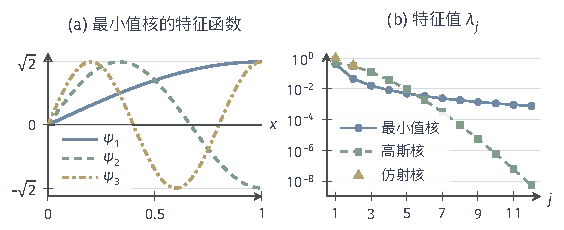
\includegraphics[width=95.5mm]{figures/02-abstract-mathematics/03-function-spaces/tikz/c5-mercer-spectrum/figure.pdf}
  \caption{Mercer特征函数与特征值衰减。(a)~最小值核在$[0,1]$、Lebesgue测度下的前三个特征函数$\psi_j=\sqrt2\sin((j-\frac12)\pi x)$，它们在$0$处为零、在$1$处导数为零；(b)~特征值（对数纵轴）：最小值核$\lambda_j=((j-\frac12)\pi)^{-2}$；高斯核（$\sigma=0.5$，$[-1,1]$，$\mathrm dz/2$）的特征值由40点Gauss--Legendre求积离散计算；仿射核只有$1$与$1/3$两个正特征值。}
  \label{fig:rkhs-mercer-spectrum}
\end{figure}

\subsection{RKHS中的谱坐标}
\label{sec:rkhs-spectral-coordinates}

Mercer展开把核写成了一族加权特征的内积：令$\Phi(x)=\bigl(\sqrt{\lambda_j}\,\overline{\phi_j(x)}\bigr)_j\in\ell^2$，则$\langle\Phi(x),\Phi(y)\rangle_{\ell^2}=\sum_j\lambda_j\phi_j(x)\overline{\phi_j(y)}=K(x,y)$。代入定理~\ref{thm:rkhs-feature-space}，就能读出RKHS在谱坐标下的形式。

\begin{theorem}[RKHS的谱表示]
\label{thm:rkhs-spectral-norm}
在定理~\ref{thm:rkhs-mercer}的条件下：
\begin{enumerate}
\item $\{\sqrt{\lambda_j}\,\phi_j\}$是$H_K$的标准正交基；
\item 函数$f:X\to\mathbb K$属于$H_K$，当且仅当存在数列$(a_j)$满足$\sum_j\lvert a_j\rvert^2/\lambda_j<\infty$，且$f(x)=\sum_ja_j\phi_j(x)$对一切$x$成立。此时级数在$X$上绝对一致收敛，$a_j=\langle\phi_j,f\rangle_{L^2(\mu)}$，并且
\begin{equation}
\lVert f\rVert_{L^2(\mu)}^2=\sum_j\lvert a_j\rvert^2,\qquad \lVert f\rVert_{H_K}^2=\sum_j\frac{\lvert a_j\rvert^2}{\lambda_j}.
\label{eq:rkhs-two-norms}
\end{equation}
\end{enumerate}
\end{theorem}

\begin{proof}
由定理~\ref{thm:rkhs-mercer}，$\lVert\Phi(x)\rVert^2=K(x,x)<\infty$，$\Phi$是$K$的特征映射，对应的函数为$f_w(x)=\langle\Phi(x),w\rangle=\sum_jw_j\sqrt{\lambda_j}\,\phi_j(x)$。先证$\Phi(X)$张成的闭子空间是整个$\ell^2$。设$w\in\ell^2$与每个$\Phi(x)$正交，即$\sum_jw_j\sqrt{\lambda_j}\phi_j(x)=0$对一切$x$成立。系数$w_j\sqrt{\lambda_j}$平方可和，同一级数在$L^2(\mu)$中收敛，其$L^2$极限有一个子列几乎处处收敛到它，所以$L^2$极限为零；由$\phi_j$的标准正交性，$w_j\sqrt{\lambda_j}=0$，即$w=0$。

于是由定理~\ref{thm:rkhs-feature-space}，$w\mapsto f_w$是从$\ell^2$到$H_K$的等距同构，单位向量$e_j$映为$\sqrt{\lambda_j}\phi_j$，这证明第1条。令$a_j=\sqrt{\lambda_j}\,w_j$，条件$w\in\ell^2$就是$\sum_j\lvert a_j\rvert^2/\lambda_j<\infty$，且$\lVert f_w\rVert_{H_K}^2=\sum_j\lvert w_j\rvert^2$。一致收敛来自
\[
\Bigl\lvert\sum_{j>m}a_j\phi_j(x)\Bigr\rvert\leq\Bigl(\sum_{j>m}\frac{\lvert a_j\rvert^2}{\lambda_j}\Bigr)^{1/2}\Bigl(\sum_{j>m}\lambda_j\lvert\phi_j(x)\rvert^2\Bigr)^{1/2}\leq\kappa\Bigl(\sum_{j>m}\frac{\lvert a_j\rvert^2}{\lambda_j}\Bigr)^{1/2} .
\]
一致收敛的级数也在$L^2(\mu)$中收敛到同一函数，由标准正交性得$a_j=\langle\phi_j,f\rangle_{L^2}$与$\lVert f\rVert_{L^2}^2=\sum_j\lvert a_j\rvert^2$。
\end{proof}

\paragraph{两种范数的坐标权重}

式~\eqref{eq:rkhs-two-norms}说明，同一组谱坐标$a_j$在两种范数中得到不同的权重：$L^2$范数对每个坐标一视同仁，RKHS范数把第$j$个坐标的平方放大$1/\lambda_j$倍。$L^2$中的单位方向$\phi_j$在$H_K$中的长度是$\lambda_j^{-1/2}$，$H_K$中真正的单位方向是$\sqrt{\lambda_j}\phi_j$。由于$\lambda_j\to0$，特征值小的方向在RKHS范数中代价很高。

对最小值核，$1/\lambda_j=\omega_j^2$，$\lVert f\rVert_{H_{\min}}^2=\sum_j\omega_j^2\lvert a_j\rvert^2$，这正是$\lVert f'\rVert_{L^2}^2$在余弦基$\sqrt2\cos(\omega_jx)$下的展开。图~\ref{fig:rkhs-norm-weights}中，$f=\phi_1$与$g=\phi_1+0.1\phi_8$的图像几乎重合，$\lVert f-g\rVert_{L^2}=0.1$；但$\lVert f-g\rVert_{H_{\min}}=0.1\,\omega_8=0.75\pi\approx2.36$，比$\lVert f\rVert_{H_{\min}}=\omega_1\approx1.57$还大。高频的小波纹带来很大的导数。

\begin{figure}[!htb]
  \centering
  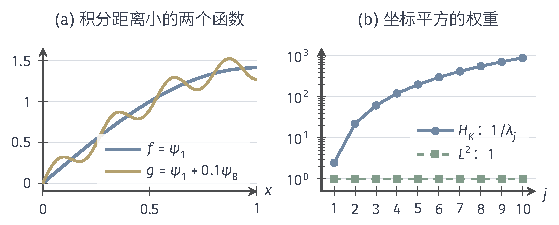
\includegraphics[width=94.6mm]{figures/02-abstract-mathematics/03-function-spaces/tikz/c5-norm-weights/figure.pdf}
  \caption{最小值核下两种范数的谱权重（图中$\psi_j$即正文的$\phi_j$）。(a)~$f=\psi_1$与$g=\psi_1+0.1\psi_8$，$\psi_j=\sqrt2\sin((j-\frac12)\pi x)$；两者的$L^2$距离为$0.1$，核范数距离却约为$2.36$。(b)~谱坐标平方在两种范数中的权重：$L^2$中恒为$1$，$H_K$中为$1/\lambda_j=((j-\frac12)\pi)^2$（对数纵轴），随$j$平方增长。}
  \label{fig:rkhs-norm-weights}
\end{figure}

\paragraph{只使用非零特征方向}

定理~\ref{thm:rkhs-spectral-norm}对$H_K$的成员提出两项要求：作为$L^2$元素，函数没有零特征值方向的分量；谱坐标的加权平方和有限。两项要求可以分别不满足。仿射核下，$x^2=\tfrac13\phi_1+(x^2-\tfrac13)$含有零空间分量$x^2-\tfrac13$，所以不在$H_{\mathrm{aff}}$中。最小值核下零空间平凡，但常数$1$的谱坐标为$a_j=\sqrt2/\omega_j$，$\sum_j\lvert a_j\rvert^2=1$有限，$\sum_j\lvert a_j\rvert^2/\lambda_j=\sum_j2$却发散；常数$1$在$L^2$中有谱展开，却不属于$H_{\min}$，这与$H_{\min}$要求$f(0)=0$相符。

\paragraph{谱坐标依赖测度，RKHS范数不依赖}

仍取仿射核，把$[-1,1]$上的测度从$\mathrm dx/2$换成$\mathrm dx$，特征值变为$2$与$\tfrac23$，标准正交特征函数变为$1/\sqrt2$与$\sqrt{3/2}\,x$。对$f=a+bx$，新的谱坐标为$a_1=\sqrt2\,a$，$a_2=\sqrt{2/3}\,b$，于是
\[
\frac{\lvert a_1\rvert^2}{\lambda_1}+\frac{\lvert a_2\rvert^2}{\lambda_2}=\frac{2a^2}{2}+\frac{2b^2/3}{2/3}=a^2+b^2 ,
\]
与原来的RKHS范数相同；而$L^2$范数平方从$a^2+b^2/3$变成了$2a^2+2b^2/3$。一般地，由定理~\ref{thm:rkhs-moore-aronszajn}，$H_K$的内积只由核决定；测度提供的是一组正交坐标和积分意义下的误差度量。

\subsection{Mercer谱特征的截断}
\label{sec:rkhs-spectral-truncation}

谱坐标给出一种由核与测度共同确定的有限特征：按非增的特征值保留前$N$个非零谱方向$\phi_1,\ldots,\phi_N$，令$V_N=\operatorname{span}\{\phi_1,\ldots,\phi_N\}$，把$f=\sum_ja_j\phi_j$截断为$f_N=\sum_{j\leq N}a_j\phi_j$。因为$\phi_j$在$L^2(\mu)$与$H_K$两种内积下都两两正交，$f_N$同时是$f$在$V_N$上的$L^2$投影与$H_K$投影。

\paragraph{两种尾和}

由式~\eqref{eq:rkhs-two-norms}，两种范数下的截断误差都是系数的尾和，只是权重不同：
\begin{equation}
\lVert f-f_N\rVert_{H_K}^2=\sum_{j>N}\frac{\lvert a_j\rvert^2}{\lambda_j},\qquad
\lVert f-f_N\rVert_{L^2(\mu)}^2=\sum_{j>N}\lvert a_j\rvert^2 .
\label{eq:rkhs-tail-sums}
\end{equation}
若$T_K$只有$r$个非零特征值（有限秩），则$H_K=V_r$是$r$维的，保留全部$r$个非零方向即可精确表示$H_K$中的每个函数，例如仿射核取$N=2$。下面考虑无穷多个非零特征值的情形。

\paragraph{单位球上的$L^2$误差}

对$j>N$有$\lambda_j\leq\lambda_{N+1}$，所以
\begin{equation}
\lVert f-f_N\rVert_{L^2(\mu)}^2=\sum_{j>N}\lambda_j\cdot\frac{\lvert a_j\rvert^2}{\lambda_j}\leq\lambda_{N+1}\lVert f-f_N\rVert_{H_K}^2\leq\lambda_{N+1}\lVert f\rVert_{H_K}^2 .
\label{eq:rkhs-tail-comparison}
\end{equation}
因此对RKHS单位球中的全部函数，$L^2$平方误差有统一的上界$\lambda_{N+1}$，随$N\to\infty$趋于零。这个界不能改进：$f=\sqrt{\lambda_{N+1}}\phi_{N+1}$的RKHS范数为$1$，$L^2$平方误差恰好是$\lambda_{N+1}$。

这个统一界依赖于两种范数的差别，在RKHS范数下没有对应的结论。仍取$f=\sqrt{\lambda_{N+1}}\phi_{N+1}$，它与$V_N$正交，$\lVert f-f_N\rVert_{H_K}=\lVert f\rVert_{H_K}=1$。所以对每个$N$，单位球中总有函数的RKHS截断误差等于$1$，不能推出单位球在RKHS范数下有统一趋零的截断误差。对单个固定的$f\in H_K$，式~\eqref{eq:rkhs-tail-sums}中的RKHS尾和仍趋于零，只是趋于零的速度取决于$f$本身。

\paragraph{逐点误差与核的截断}

RKHS误差还控制逐点误差。$V_N$的再生核是$K_N(x,y)=\sum_{j\leq N}\lambda_j\phi_j(x)\overline{\phi_j(y)}$，由定理~\ref{thm:rkhs-subspace-error}，
\begin{equation*}
\begin{gathered}
\lvert f(x)-f_N(x)\rvert\leq\sqrt{R_N(x)}\,\lVert f-f_N\rVert_{H_K},\\
R_N(x)=K(x,x)-K_N(x,x)=\sum_{j>N}\lambda_j\lvert\phi_j(x)\rvert^2 .
\end{gathered}
\end{equation*}
由Mercer定理，$R_N$一致趋于零，$\int_XR_N\,\mathrm d\mu=\sum_{j>N}\lambda_j$。所以截断后的核$K_N$在$X\times X$上一致逼近$K$，这是核的近似；某个具体函数的误差还要乘上它自己的RKHS尾和。

\begin{example}[最小值核的三项截断]
\label{ex:rkhs-hmin-truncation}
取$q(x)=4x(1-x)\in H_{\min}$。两次分部积分给出谱坐标$a_j=4\sqrt2\bigl(2\omega_j^{-3}-(-1)^{j+1}\omega_j^{-2}\bigr)$，前三项约为$0.626$、$0.363$、$-0.068$。又$\lVert q\rVert_{L^2}^2=\tfrac{8}{15}$，$\lVert q\rVert_{H_{\min}}^2=\tfrac{16}{3}$，用总和减去前三项，得
\[
\lVert q-q_3\rVert_{L^2}\approx0.068,\qquad \lVert q-q_3\rVert_{H_{\min}}\approx1.07 .
\]
核对式~\eqref{eq:rkhs-tail-comparison}：$0.068^2\approx0.0046\leq\lambda_4\times1.07^2\approx0.0083\times1.15\approx0.0095$。RKHS尾和远大于$L^2$尾和，因为$q'(1)=-4\neq0$，而每个$\phi_j$在$1$处导数为零，谱坐标只按$\omega_j^{-2}$衰减。

与例~\ref{ex:rkhs-hmin-interpolation}比较：三个核截面的折线插值，RKHS误差为$\sqrt{16/27}\approx0.77$，小于三项谱截断的$1.07$。核的积分误差则相反：$\int_0^1R_3\,\mathrm dx=\tfrac12-\sum_{j\leq3}\omega_j^{-2}\approx0.034$，小于三个节点的幂函数平方的积分$\int_0^1P_{Z_3}(x)^2\,\mathrm dx=\tfrac{h}{6}=\tfrac1{18}\approx0.056$（由例~\ref{ex:rkhs-hmin-grid}的公式在每个小区间上积分）。两种三维子空间各有所长，哪一种更好取决于所用的误差度量。
\end{example}

谱截断需要先求解积分算子的特征问题，而测度在实际中常常未知或只能由样本给出。由样本点构造Gram矩阵并作谱分解，得到的是第~\ref{sec:rkhs-section-span-approx}节的核截面子空间及其投影核，而不是这里的$K_N$；二者之间的关系涉及抽样误差，本节的尾和结论不能自动搬到这类数值方法上。

\section{本章小结}
\label{sec:rkhs-summary}

章首的问题是：有限个点值怎样约束一条函数。本章的回答从候选空间开始。有限特征空间把插值化为设计矩阵方程，但维数一变，可行性与唯一性随之改变，零残差也不保证测点之外的误差为零。要在无限维空间中选函数，候选空间必须让点值有确定意义且受范数控制；$L^2$两项都不满足，$H^1(0,1)$与$H_{\min}$都满足。

把每个点评估都连续的Hilbert函数空间称为RKHS之后，Riesz表示把读数写成与核截面的内积$f(x)=\langle K_x,f\rangle$，核截面的内积就是再生核。再生核共轭对称、正定，对角值$K(x,x)$给出点评估的范数，核截面的组合在空间中稠密。反过来，任何正定核经过半内积、零范数商与完备化，唯一确定一个以它为再生核的RKHS；补进来的极限元素由点值估计识别为函数。新核可以由特征映射、非负线性组合与逐点乘积得到，同一个核可以有维数不同的特征表示，RKHS的范数等于能给出该函数的最短参数长度。

有限观测问题由观测映射$S$与Gram矩阵$\bm G=SS^*$完整描述。观测零空间$N=\ker S$与核截面张成的$M$互为正交补，投影到$M$保留读数而不增大范数。数据可插值当且仅当$\bm y$属于$\bm G$的像；可行时，最小范数插值$f^+=\sum_jc_jK_{x_j}$唯一，即使$\bm G$奇异、系数不唯一也是如此。没有插值函数与插值函数不唯一由不同对象决定，前者看$\bm G$的像，后者看$N$。

表示误差的比较必须说明在哪个空间、用哪些观测、按哪个范数。在RKHS内，子空间$V$的投影误差乘以$\sqrt{K(x,x)-K_V(x,x)}$控制逐点误差；核截面的坐标由点值读出，限定点集的截面是否稠密取决于核的连续性与点集是否足以排除非零函数。一般有限特征可以更经济，但其欧氏内积给出的有限特征核不是原核，原空间中子空间的核要按$H$的Gram矩阵加权。

加入全支撑的有限测度后，紧度量空间上连续正定核的积分算子是紧、自伴、正算子，Mercer定理给出核的绝对一致展开$K(x,y)=\sum_j\lambda_j\phi_j(x)\overline{\phi_j(y)}$。$\{\sqrt{\lambda_j}\phi_j\}$是RKHS的标准正交基，同一组谱坐标在$L^2$与RKHS中的权重相差$1/\lambda_j$。截断前$N$个谱方向时，RKHS单位球上的$L^2$平方误差统一不超过$\lambda_{N+1}$，RKHS误差却没有统一趋零的界。读数带噪声时的损失与正则化选择属于卷五，随机观测的统计误差属于卷八；它们使用的正是本章的正交分解与有限表示。


